\documentclass[11pt,a4paper,twoside,openright]{memoir}


%%% PREAMBULES %%%
\usepackage[utf8]{inputenc}
\usepackage[T1]{fontenc}


% POLICES
\usepackage{lmodern} % lmodern pour le mode math...
\edef\oldtt{\ttdefault} % et le mode typewriter
\usepackage[oldstyle, proportional]{libertine} % libertine comme police principale
\renewcommand{\ttdefault}{\oldtt}
\usepackage[scaled=0.875]{helvet} % helvetica comme police sans serif
\usepackage{slantsc} % slanted small caps

% preambules
% Page layout (margins)
%\usepackage[margin=28mm,includeheadfoot,bindingoffset=5mm]{geometry}

\settrimmedsize{297mm}{210mm}{*}
\setlength{\trimtop}{0pt} 
\setlength{\trimedge}{\stockwidth} 
\addtolength{\trimedge}{-\paperwidth} 

% si no de page en bas
% \setlrmarginsandblock{3.25cm}{*}{*} % spine, edge, edge-to-spine ratio
% \setulmarginsandblock{3.0cm}{*}{1.25} % upper, lower, lower-to-upper ratio
% \setheadfoot{\onelineskip}{2\onelineskip}
% \checkandfixthelayout 


% si no de page en haut
\setlrmarginsandblock{3.2cm}{*}{*} % spine, edge, edge-to-spine ratio
\setulmarginsandblock{3.0cm}{*}{} % upper, lower, lower-to-upper ratio
\setheadfoot{\onelineskip}{\onelineskip}
\checkandfixthelayout 


% Show page margins, \usepackage[noframe]{showframe} to disable
\usepackage[noframe]{showframe}
%https://tex.stackexchange.com/questions/328662/showframe-how-to-make-colored-lines-of-page-layout
\renewcommand*\ShowFrameColor{\color{red}} % marges
\usepackage{color,xcolor}

%\colorlet{mydarkgray}{black!84}
\definecolor{mydarkgray}{HTML}{212131}%111122}

\definecolor{DodgerBlue3}{rgb}{0.094, 0.455, 0.804}
\definecolor{bleuONERA1}{rgb}{0.09,0.40,1.00} % Bleu du logo Onera
\definecolor{bleuONERA2}{rgb}{0.0,0.33,0.66}  % Bleu de la gauche du bandeau haut
\definecolor{bleuONERA3}{rgb}{0.85,0.90,0.95} % Bleu de la droite du bandeau haut

\definecolor{deepblue}{rgb}{0.0, 0.212, 0.596}

\definecolor{myred}{rgb}{0.8431,0.1882,0.1529}
\definecolor{mygreen}{rgb}{0.2118,0.6118,0.0235}


\definecolor{redlink}{HTML}{CD463C}
\definecolor{blulink}{HTML}{3C5FCC}

\definecolor{greenlink}{HTML}{198C32}



%%%%%%%%%
\definecolor{sunset01}{HTML}{364B9A}
\definecolor{sunset02}{HTML}{4A7BB7}
\definecolor{sunset03}{HTML}{6EA6CD}
\definecolor{sunset04}{HTML}{98CAE1}
\definecolor{sunset05}{HTML}{C2E4EF}
\definecolor{sunset06}{HTML}{EAECCC}
\definecolor{sunset07}{HTML}{FEDA8B}
\definecolor{sunset08}{HTML}{FDB366}
\definecolor{sunset09}{HTML}{F67E4B}
\definecolor{sunset10}{HTML}{DD3D2D}
\definecolor{sunset11}{HTML}{A50026} % couleurs prédéfinies
%https://tex.stackexchange.com/questions/50747/options-for-appearance-of-links-in-hyperref
\usepackage[pagebackref]{hyperref} % hyper link to page where reference is cited
\renewcommand*{\backrefsep}{, }
\renewcommand*{\backreflastsep}{ et }
\renewcommand*{\backreftwosep}{ et }
\renewcommand*{\backref}[1]{}
\renewcommand*{\backrefalt}[4]{%
    \ifcase #1 {\color{red}(Pas cité)}%\relax%
    \or        (\cf p.~#2)%
    \else      (\cf pp.~#2)%
    \fi}

\hypersetup{
	breaklinks,
	colorlinks=true,
	linkcolor=DodgerBlue3,
	anchorcolor=myred,%DarkRed,%
    citecolor=DodgerBlue3,%redlink,%black,%mygreen,
	pdfdisplaydoctitle=true,
	pdfpagemode=UseOutlines,%
	bookmarksnumbered=true,
	bookmarksopen=true,
	hypertexnames=true,
	linktoc=all
}
    
\usepackage{memhfixc} % Must be used on memoir document class after hyperref (?)



% Adding package bookmark improves bookmarks handling.
% More features and faster updated bookmarks.
%https://tex.stackexchange.com/questions/65544/how-to-link-table-of-contents-in-thesis-pdf
\usepackage{bookmark}


\renewcommand*{\sectionrefname}{Section~}
\renewcommand*{\chapterrefname}{Chapitre~}
\renewcommand*{\partrefname}{Partie~}
\renewcommand*{\appendixrefname}{Appendice~}
\newcommand{\algorithmautorefname}{Algorithme} % format des liens et références croisées
\usepackage{graphicx}


\usepackage{tikz}
\usetikzlibrary{calc}

\makeatletter
\newcommand{\gettikzxy}[3]{%
  \tikz@scan@one@point\pgfutil@firstofone#1\relax
  \edef#2{\the\pgf@x}%
  \edef#3{\the\pgf@y}%
}

\newcommand{\globalgettikzxy}[3]{%
  \tikz@scan@one@point\pgfutil@firstofone#1\relax
  \edef\@tempdima{\the\pgf@x}%
  \edef\@tempdimb{\the\pgf@y}%
  \global#2=\@tempdima%
  \global#3=\@tempdimb%
}

\newcommand\getwidthofnode[2]{%
    \pgfextractx{\pgf@xb}{\pgfpointanchor{#2}{east}}%
    \pgfextractx{\pgf@xa}{\pgfpointanchor{#2}{west}}% 
    \pgfmathsetlength{\pgf@xb}{\pgf@xb - \pgf@xa}%
	\global#1=\pgf@xb%
}

\newcommand\getheightofnode[2]{%
    \pgfextracty{\pgf@yb}{\pgfpointanchor{#2}{north}}%
    \pgfextracty{\pgf@ya}{\pgfpointanchor{#2}{south}}% 
    \pgfmathsetlength{\pgf@yb}{\pgf@yb - \pgf@ya}%
	\global#1=\pgf@yb%
}
\makeatother




% chemin(s) des figures
\graphicspath{{./figures/}}%,{../fig2/}}


% controle des objets flottants (figures, tables)
\renewcommand{\topfraction}{0.7}     % autorise 70% page de graphique en haut
\renewcommand{\bottomfraction}{0.5}  % autorise 50% page de graphique en bas
\renewcommand{\floatpagefraction}{0.7}
\renewcommand{\textfraction}{0.1} % TikZ, PGF, PStricks
% Math packages, notations
\usepackage{amsthm}
\usepackage{amssymb}
\usepackage{amsmath}    % amsmath equation env has funny spacing with hyperref :-( so...
\let\equation\gather \let\endequation\endgather
\usepackage{amsfonts}
\usepackage{bm}
\usepackage{mathtools}
\usepackage{stmaryrd}

%https://tex.stackexchange.com/questions/165685/subequations-and-array-in-braces
\usepackage[overload]{empheq}

\usepackage{cases}

\usepackage{esint}
\usepackage[overload]{empheq}%https://tex.stackexchange.com/questions/165685/subequations-and-array-in-braces

\usepackage{xifthen}% provides \isempty test
\usepackage{xparse}
\usepackage{xstring}

\usepackage{mathrsfs}% script (mathscr}

% *** TWEAK (NEGATIVE) SPACES *** 
%https://tex.stackexchange.com/questions/67912/large-negative-spaces
%https://tex.stackexchange.com/questions/9091/what-is-the-right-way-to-use-the-spacing-command/9092

%https://tex.stackexchange.com/questions/2783/bold-calligraphic-typeface
\DeclareMathAlphabet\matholdcal{OMS}{cmsy}{m}{n}

%https://tex.stackexchange.com/questions/247531/how-to-use-boondox-calligraphic-font-in-latex-without-replacing-mathcal-command/247819
%https://ctan.org/pkg/mathalfa
\usepackage[
scr=boondoxo, scrscaled=1.05, 
cal=zapfc, calscaled=1.18%,
%frak=mma, frakscaled=1.,
]{mathalfa}


%https://tex.stackexchange.com/questions/399620/how-can-i-get-a-bar-over-a-subscript
\usepackage{widebar}


%https://tex.stackexchange.com/questions/234676/new-theorem-style
%https://en.wikibooks.org/wiki/LaTeX/Theorems
\newtheoremstyle%
   {mythm}% name of the style to be used
   {\topsep}% measure of space to leave above the theorem. E.g.: 3pt
   {\topsep}% measure of space to leave below the theorem. E.g.: 3pt
   {\itshape}% font to use in the body of the theorem
   {0pt}% measure of space to indent
   {\bfseries\scshape}% head font
   {~---}% punctuation between head and body
   { }%\newline}% space after theorem head; " " = normal interword space
   {}%{\thmname{#1}\thmnumber{ #2}\thmnote{ (#3)}}% Manually specify head
\theoremstyle{mythm}

\newtheorem{theoreme}{Théorème}[chapter]
\newtheorem{propriete}{Propriété}[chapter]
\newtheorem{definition}{Définition}[chapter]
\renewcommand{\proofname}{Preuve}
\renewcommand\qedsymbol{$\blacksquare$}%{C.Q.F.D.}%

% Notations
\newcommand*{\rank}[1]{\mathrm{rang}{#1}}
\newcommand*{\determinant}[1]{\det{#1}}%{\left\lvert {#1} \right\rvert}
\newcommand*{\inv}[1]{#1\raisebox{1.15ex}{$\scriptscriptstyle-\!1$}}
\newcommand*{\inverse}[1]{\ensuremath{{#1} ^{-1}}} % inverse matrix
\newcommand*{\transpose}[1]{\ensuremath{{#1} ^\mathsf{T}}} % transpose matrix
\newcommand*{\dotprod}[2]{ \transpose{#1} {#2} } % dot product
\newcommand*{\crossprod}[2]{ {#1} \times {#2} } % cross product
\newcommand*{\normtwo}[1]{ \left\| {#1} \right\| } % Euclidean norm
\newcommand*{\norminf}[1]{ \left\| {#1} \right\|_{\infty} } % infinity norm
\newcommand*{\vit}[1]{\bm{#1}} % greek letter vector
\newcommand*{\vrm}[1]{\mathbf{#1}} % latin letter vector
\newcommand*{\unitized}[1]{ \frac{#1}{\normtwo{#1}} }
\newcommand*{\scalprod}[2]{\left \langle {#1}, {#2} \right \rangle}
\newcommand*{\modulo}[1]{\pmod{#1}}%{\left[ {#1} \right]}

\DeclareMathOperator*{\argmin}{\arg\!\min} % argmin
\DeclareMathOperator*{\sign}{sign} % argmin

\newcommand*{\bigO}[1]{O\!\left( {#1} \right)} % big-O
\newcommand*{\littleo}[1]{o\!\left( {#1} \right)} % little-o

% sets
\newcommand*{\reals}{\ensuremath{\mathbb{R}}}
\newcommand*{\integers}{\ensuremath{\mathbb{N}}}
\newcommand{\family}[4]{\left\{{#1}_{#2}\right\}_{{#2}={#3},\ldots,{#4}}}
\newcommand{\ffamily}[7]{\left\{{#1}_{#2,#5}\right\}_{\substack{{#2}={#3},\ldots,{#4}\\ \substack{{#5}={#6},\ldots,{#7}}}}}
\newcommand{\polyspace}[1]{\Pi_{#1}}%\mathbb{R}_{#1}[x]}
\newcommand{\Ltwospace}{L^2\chebinterval}%\mathcal{L}_2\chebinterval}
\newcommand*{\contdiff}[1]{\ensuremath{C^{#1}}}%{\matholdcal{C}^{#1}\!}
\newcommand*{\contgeom}[1]{\ensuremath{G^{#1}}}%{\matholdcal{G}^{#1}\!}

\newcommand*{\uvdomain}{\ensuremath{\mathcal{U}}}
\newcommand*{\wdomain}{\ensuremath{\mathcal{W}}}

\newcommand*{\bx}{\vit{x}}
\newcommand*{\bu}{\vit{u}}
\newcommand*{\bd}{\vit{\delta}}
\newcommand*{\bg}{\vit{\gamma}}
\newcommand*{\bgw}{\bg_{\mkern-2muw}}
\newcommand*{\bp}{\vit{\psi}}
\newcommand*{\bpw}{\bp_{\mkern-2muw}}
\newcommand*{\bl}{\vit{\lambda}}
\renewcommand*{\bs}{\vit{\sigma}} % originally backslash in typewriter font
\newcommand*{\bsu}{\bs_{\mkern-3muu}}
\newcommand*{\bsv}{\bs_{\mkern-2muv}}
\newcommand{\bt}{\vrm{t}}
\newcommand{\br}{\vrm{r}}
\newcommand{\bo}{\vit{o}}

\newcommand*{\unv}{\vrm{n}} % unit normal vector
\newcommand*{\nv}{\hat{\unv}} % normal vector



\newcommand{\colvec}[1]{\begin{pmatrix} #1 \end{pmatrix}} % vector printed in column
\newcommand{\rowvec}[1]{ \transpose{\begin{pmatrix} #1 \end{pmatrix}} } % vector printed in row (transposed column)

% Differential operators
\newcommand*{\dfdx}[2]{\frac{\mathrm{d}}{\mathrm{d}{#2}}{#1}}
\newcommand*{\partialdfdx}[2]{\frac{\partial}{\partial{#2}}{#1}}
\newcommand*{\dkfdxk}[3]{\frac{\mathrm{d}^{#3}}{\mathrm{d}{#2}^{#3}}{#1}}
\newcommand*{\deriv}[2]{{#1}^{({#2})}}
\newcommand*{\prim}[2]{{#1}^{(\raisebox{0.2ex}{$\scriptscriptstyle-\!$}{#2})}}
\newcommand*{\jacobian}[1]{\mathbf{J}_{#1}}
\newcommand*{\gradient}[1]{\nabla \! {#1}}
\newcommand*{\hessian}[1]{\mathbf{H}_{#1}}
\newcommand*{\divergence}[1]{\nabla \cdot {#1}}%\mathrm{div}{#1}}
\newcommand*{\dx}[1]{\mathrm{d}{#1}}



% Condition number
\newcommand*{\cond}[1]{\mathrm{cond} \! \left( {#1} \right)}

% Differential geometry
\newcommand{\fff}{\mathbf{I}}     % first fundamental form
\newcommand{\sffc}{I\mkern-4.8muI} % second fundamental form coefs
\newcommand{\sff}{\mathbf{I\!I}} % second fundamental form




%% Chebyshev polynomials
% Reference interval
\newcommand*{\chebinterval}{\ensuremath{\left[ -1, 1 \right]}}
\newcommand*{\chebopeninterval}{\ensuremath{\left] -1, 1 \right[}}
\newcommand*{\series}[1]{S{#1}}
\newcommand*{\truncseries}[2]{P_{#2}{#1}}
\newcommand*{\interpolant}[2]{I_{#2}{#1}}
\newcommand*{\interpderiv}[3]{D_{#2}^{(#3)}{\!#1}}%\mathcal{D}
%\newcommand*{\interpprim}[2]{J_{#2}{#1}}
\newcommand*{\interpprim}[2]{D_{#2}^{(\raisebox{0.2ex}{$\scriptscriptstyle-\!$}1)}{\!#1}}

% Reference interval for Bernstein polynomials
\newcommand*{\berninterval}{\left[ 0, 1 \right]}

%% System of equations
\newenvironment{eqsys}
{\left\lbrace\begin{array}{@{}l@{}}}
{\end{array}\right.}
%ex :
%\begin{equation}
%	\begin{eqsys}
%		y_1 = a_1 x + b_1 \\
%		y_2 = a_2 x + b_2
%	\end{eqsys}
%\end{equation}


% Intervals
\newcommand*{\lo}[1]{\underline{#1}}
\newcommand*{\hi}[1]{\widebar{#1}}%\overline{#1}}


% GRAPHS
\DeclareMathOperator{\orig}{orig}%ine}
\DeclareMathOperator{\dest}{dest}%ination}



% ENVELOPES OF SPHERES/BALLS
%\newcommand*{\sphere}[2]{\mathscr{S}(#1,#2)}                   % sphère
\newcommand*{\spherenotation}{\mathscr{S}}
\NewDocumentCommand{\sphere}{o o}{%
	\IfValueTF{#1}{%
		\IfValueTF{#2}{%
			\ensuremath{\spherenotation(#1,#2)}%
		}{%
			\ensuremath{\spherenotation(#1)}%
		}%
	}{%
		\ensuremath{\spherenotation}%
	}%
}

\newcommand*{\ball}[2]{\mathscr{B}(#1,#2)}                     % boule ouverte
\newcommand*{\implicitsphere}{S}                               % fonction définissant implicitement une sphère
\newcommand*{\implicitEdB}[1]{\varphi_{#1}}                    % fonction définissant implicitement une EdB
\newcommand*{\EdB}[2]{{#1}^{#2}}                               % EdB
%\newcommand*{\EoS}[2]{\widehat{\EoB{#1}{#2}}}                  % EdS
\newcommand*{\influ}{\mathscr{I}}                              % zone d'influence
\newcommand*{\influEdB}[2]{\influ^{\!#2}({#1})}                % zone d'influence sur l'EdB
%\newcommand*{\influEoS}[2]{\widehat{\influ}^{\!#2}({#1})}      % zone d'influence sur l'EdS
%\newcommand*{\properEoB}[2]{\influ_*^{\!#2}({#1})}             % EdB propre
%\newcommand*{\properEoS}[2]{\widehat{\influ}_{*}^{\!#2}({#1})} % EdS propre
\newcommand*{\eos}{\vit{e}}                                    % paramétrisation de l'EdS (propre)
\newcommand*{\dilation}[2]{{#1}_{\uparrow #2}}                 % "dilatation"

\newcommand*{\envelope}{\mathcal{E}}
\newcommand*{\EdS}[2]{{\envelope}^{#2}({#1})}                  % EdS
\newcommand*{\EdSpropre}[2]{{\envelope}_{*}^{#2}({#1})}        % EdS propre
\newcommand*{\EdSpropreplus}[2]{{\envelope}_{+}^{#2}({#1})}    % EdS propre "positive"
\newcommand*{\EdSpropremoins}[2]{{\envelope}_{-}^{#2}({#1})}   % EdS propre "négative"
\newcommand*{\pseudoEdS}[2]{\widehat{\envelope}^{#2}({#1})}    % pseudo-EdS

\newcommand*{\circlenotation}{\mathscr{C}}

% SET THEORY/TOPOLOGY
\newcommand*{\closure}[1]{\widebar{#1}}%\mathrm{cl}#1}%
\newcommand*{\interior}[1]{\mathrm{int}{#1}}%\mathring{#1}}%
\newcommand*{\boundary}[1]{\partial #1}
\renewcommand*{\complement}[1]{#1^\mathsf{C}}
\newcommand*{\neigborhood}{\mathscr{V}}



%\newcommand*{\proof}[1]{\textcolor{blue!60!green}{\textbf{Preuve : }#1$\,_\blacksquare$}}



% Encircled text
\newcommand{\pgftextcircled}[1]{                                                                    
    \setbox0=\hbox{#1}%
    \dimen0\wd0%
    \divide\dimen0 by 2%
    \begin{tikzpicture}[baseline=(a.base)]%
        \useasboundingbox (-\the\dimen0,0pt) rectangle (\the\dimen0,1pt);
        \node[circle,draw,outer sep=0pt,inner sep=0.1ex] (a) {#1};
    \end{tikzpicture}
}

 % notations mathématiques
\newboolean{titlerectangle}
\setboolean{titlerectangle}{true}

\newboolean{titlevbar}
\setboolean{titlevbar}{true}

\newboolean{titlehelpers}
\setboolean{titlehelpers}{true}

\newboolean{sansseriftitles}
\setboolean{sansseriftitles}{false}

\ifthenelse{\boolean{sansseriftitles}}{
	\def\titlefont{\sffamily}%
}
{
	\def\titlefont{\rmfamily}%
}

% Table of contents style
\renewcommand*{\contentsname}{Table of contents}
\renewcommand*{\cftchapterfont}{\titlefont\bfseries}



\maxtocdepth{subsection}

% Titles
\colorlet{colchapttl}{mydarkgray}%black}%DodgerBlue3}%



\makeatletter
\makechapterstyle{mychapterstyle}{
\setlength{\beforechapskip}{0pt}%40pt}
\setlength{\midchapskip}{0pt}%25pt}
\newlength{\afterchapskipdef}
\newlength{\afterchapskipxtra}
\setlength{\afterchapskipdef}{8\onelineskip}%60pt}%

\newif\ifNoChapNumber
\newlength{\barheight}
\newlength{\barlength}
\newlength{\ttltopskip}
\setlength{\ttltopskip}{60mm}
\setlength{\barlength}{0.37\foremargin}
\setlength{\barheight}{14mm}

\newlength{\numberheight}
\ifthenelse{\boolean{sansseriftitles}}{
	\setlength{\numberheight}{1.6\barheight}
}
{
	\setlength{\numberheight}{1.63\barheight}
}

\newlength{\yshiftchapname}
\newlength{\yshiftchapnum}
\setlength{\yshiftchapname}{-\ttltopskip + 10mm + 3.9mm}
\setlength{\yshiftchapnum}{-\ttltopskip - 0.1mm}

\newlength{\vbaryshift}
\setlength{\vbaryshift}{1.25mm}
\newlength{\vbarxshift}
\setlength{\vbarxshift}{2.5mm}
\newlength{\vbarthck}
\setlength{\vbarthck}{0.6pt}
\newlength{\vbartipthck}
\setlength{\vbartipthck}{0.15pt}

\renewcommand{\chapnamefont}{\scshape\titlefont}
\renewcommand{\chapnumfont}{\normalfont\titlefont\fontsize{\numberheight}{0mm}\selectfont}
\renewcommand{\chaptitlefont}{\normalfont\titlefont\bfseries\huge}%
\renewcommand{\printchaptername}{}%\chapnamefont\@chapapp}
\renewcommand{\chapternamenum}{}
\renewcommand{\printchapternum}{}


\renewcommand\printchaptertitle[1]{
	\begin{tikzpicture}[remember picture,overlay]
		\node[yshift=-\ttltopskip] at (current page.north east) {%
			\begin{tikzpicture}[remember picture, overlay]%
				%\node[%draw=red, dashed,%*****
				%	anchor=north east,%
				%	%yshift=\yshiftchapname,%
				%	%xshift=-\foremargin,%
				%	text width=\textwidth-\vbarxshift,%
				%	minimum height=\barheight,%
				%	align=flush right,%justify,%
				%	inner sep=0mm%
				%	]%
				%	(chapttl)%
				%	at ([xshift=-\foremargin-\vbarxshift, yshift=\yshiftchapname] current page.north east)%
				%	{\chaptitlefont\color{colchapttl}##1\par};%
				%
				%\draw[red, very thick, dotted] (chapttl.west) -- (chapttl.east);%*****
				%
				%\gettikzxy{(chapttl.south west)}{\bx}{\by}%
				%\global\afterchapskipxtra=-\by%
				%\pgfmathsetlength{\afterchapskip}{\afterchapskipdef + \afterchapskipxtra}%
				%\global\afterchapskip=\afterchapskip%
				%
				\ifNoChapNumber%
                                        \node[%draw=red, dashed,%*****
					anchor=north east,%
					%yshift=\yshiftchapname,%
					%xshift=-\foremargin,%
					text width=\textwidth,%
					minimum height=\barheight,%
					align=flush right,%justify,%
					inner sep=0mm%
					]%
					(chapttl)%
					at ([xshift=-\foremargin, yshift=\yshiftchapname] current page.north east)%
					{\chaptitlefont\color{colchapttl}##1\par};
					%\draw[black, thick]%
					%	([xshift=\vbarxshift, yshift= \vbaryshift] chapttl.north east)%
					%	--%
					%	([xshift=\vbarxshift, yshift=-\vbaryshift] chapttl.south east);%
					%\relax%
				\else%
                                        \node[%draw=red, dashed,%*****
					anchor=north east,%
					%yshift=\yshiftchapname,%
					%xshift=-\foremargin,%
					text width=\textwidth-\vbarxshift,%
					minimum height=\barheight,%
					align=flush right,%justify,%
					inner sep=0mm%
					]%
					(chapttl)%
					at ([xshift=-\foremargin-\vbarxshift, yshift=\yshiftchapname] current page.north east)%
					{\chaptitlefont\color{colchapttl}##1\par};%
					\node[%draw=blue, dashed,%*****
						anchor=north west,%west,%
						align=left,%
						xshift=2\vbarxshift,%
						inner sep=0mm%
						]%
						(chapnum)% 
						at (chapttl.north east)%(chapttl.east)%
						{\color{colchapttl}\chapnumfont\thechapter};%
					%
					%\draw[blue, very thick, dotted] (chapnum.west) -- (chapnum.east);%*****
					%
%\draw[colchapttl, line width=2\vbarthck]%thick]%
%([xshift=\vbarxshift, yshift= \vbaryshift] chapttl.north east)%
%--%
%([xshift=\vbarxshift, yshift=-\vbaryshift] chapttl.south east);%
%
\coordinate (a) at ([xshift=\vbarxshift+\vbartipthck,yshift=-\vbaryshift] chapttl.south east);
\coordinate (b) at ([xshift=\vbarxshift+\vbarthck]chapttl.east);
\coordinate (c) at ([xshift=\vbarxshift+\vbartipthck,yshift=+\vbaryshift] chapttl.north east);
\coordinate (d) at ([xshift=\vbarxshift-\vbartipthck,yshift=+\vbaryshift] chapttl.north east);
\coordinate (e) at ([xshift=\vbarxshift-\vbarthck]chapttl.east);
\coordinate (f) at ([xshift=\vbarxshift-\vbartipthck,yshift=-\vbaryshift] chapttl.south east);
%
\path [fill=colchapttl]%
(a) [in=0, out=90] to %
[in=270, out=90] (b) to [in=270, out=90] %
(c) -- %
(d) [in=180, out=270] to %
[in=90, out=270] (e) to [in=90, out=270] %
(f) -- cycle;
				\fi
                                \gettikzxy{(chapttl.south west)}{\bx}{\by}%
				\global\afterchapskipxtra=-\by%
				\pgfmathsetlength{\afterchapskip}{\afterchapskipdef + \afterchapskipxtra}%
				\global\afterchapskip=\afterchapskip%
			\end{tikzpicture}%
		};%
	\end{tikzpicture}%
}
\renewcommand\printchapternonum{\NoChapNumbertrue}
}
\makeatother

% helper (check if proper space after chapter title)
\newcommand{\printskip}{%
%\textbf{\the\afterchapskipdef~$+$~\the\afterchapskipxtra~$=$~\the\afterchapskip}%
}

\makeatletter
\newcommand{\printchapapp}{}%This is a \MakeLowercase{\@chapapp}.}%
\makeatother


\chapterstyle{mychapterstyle}%veelo}%











%% Format chapter abstracts
\def\abstractname{}
\def\abstitleskip{0pt}

\usepackage{lettrine}  % dropped capitals
\renewcommand{\LettrineTextFont}{\scshape}
\renewcommand{\DefaultLhang}{0.1}
\renewcommand{\DefaultNindent}{0pt}
% \renewcommand{\DefaultOptionsFile}{\lettrineconffile}



%% Sections
\setsecheadstyle{\color{colchapttl}\titlefont\Large\bfseries}%\raggedright}
\setbeforesecskip{-2\onelineskip}
\setaftersecskip{\onelineskip}
\setsecindent{0pt}

%% Subsections
\setsubsecheadstyle{\color{colchapttl}\titlefont\large\bfseries\sethangfrom{\noindent ##1}\raggedright}
\setbeforesubsecskip{-\onelineskip}
\setaftersubsecskip{\onelineskip}
\setsubsecindent{0pt}

%% Subsubsections
\setsubsubsecheadstyle{\color{colchapttl}\titlefont\bfseries\sethangfrom{\noindent ##1}\raggedright}
%\setbeforesubsubsecskip{-\onelineskip}
%\setaftersubsubsecskip{\onelineskip}
%\setsubsubsecindent{0pt}

%% Paragraphs
\setparaheadstyle{\bfseries\sethangfrom{\noindent ##1}\raggedright}
%\setbeforeparaskip{-\onelineskip}
%\setafterparaskip{-1em}
%\setparaindent{0pt} % style des titres
% Page style (header, footer) (memoir options)
\def\headingsfont{\titlefont}%\sffamily}%

% https://tex.stackexchange.com/questions/183973/preserve-memoir-headings-for-1-page
% \makeatletter
% \providecommand*{\righttopmark}{\expandafter\@rightmark\topmark\@empty\@empty}
\makepagestyle{mypagestylezero} 
\makeoddfoot{mypagestylezero}{}{}{} 
\makeevenfoot{mypagestylezero}{}{}{} 
\makeevenhead{mypagestylezero}{\thepage}{}{\headingsfont\small\leftmark}
\makeoddhead{mypagestylezero}{\itshape\headingsfont\small\rightmark}{}{\thepage}
\makepsmarks{mypagestylezero}{%
	\nouppercaseheads
	\createmark{chapter}{both}{nonumber}{}{ \ }%. \ }%
	\createmark{section}{right}{shownumber}{} { \ }
    
    \createplainmark{bib}{both}{\bibname}
    \createplainmark{toc}{both}{\contentsname}
}%
%\makeatother

\copypagestyle{mypagestyle}{mypagestylezero}
\makeheadrule{mypagestyle}{\textwidth}{\normalrulethickness} 
% \makepsmarks{mypagestyle}{%
% 	\nouppercaseheads
% 	\createmark{chapter}{left}{nonumber}{}{. \ }
% 	\createmark{section}{right}{nonumber}{} {. \ }
% }%


\copypagestyle{mypagestyleb}{mypagestyle}
\makeoddfoot{mypagestyleb}{}{}{\thepage} 
\makeevenfoot{mypagestyleb}{\thepage}{}{}
\makeevenhead{mypagestyleb}{\headingsfont\small\scshape\leftmark}{}{}
\makeoddhead{mypagestyleb}{}{}{\headingsfont\small\rightmark}



\copypagestyle{mypagestylebiblio}{mypagestyleb}
\makeoddhead{mypagestylebiblio}{}{}{\headingsfont\small\scshape\rightmark}




\makepagestyle{mypagestylenew}
\makeevenhead{mypagestylenew}{\thepage\hskip.5cm\vrule\hskip.5cm\leftmark}{}{} \makeoddhead{mypagestylenew}{}{}{\rightmark\hskip.5cm\vrule\hskip.5cm\thepage} 
\makeatletter 
\makepsmarks{mypagestylenew}{ 
  \def\chaptermark##1{\markboth{% 
  \ifnum \value{secnumdepth} < -1 %
  	\if@mainmatter \chaptername\ \thechapter\ --- %
  	\fi %
  \fi ##1}{}} 
  \def\sectionmark##1{\markright{% 
  \ifnum \value{secnumdepth} < 0 %
  	\thesection. \ %
  \fi ##1}} } 
\makeatother 




\makepagestyle{myruledpagestyle} 
%\makeevenhead{myruledpagestyle}{\liningnums{\thepage}}{}{\leftmark} \makeoddhead{myruledpagestyle}{\rightmark}{}{\liningnums{\thepage}}
\makeevenhead{myruledpagestyle}{\thepage}{}{\leftmark} \makeoddhead{myruledpagestyle}{\rightmark}{}{\thepage}
\makeatletter
\makepsmarks{myruledpagestyle}{ 
  \nouppercaseheads
  \def\chaptermark##1{\markboth{% 
    {\small\headingsfont%
    \ifnum \value{secnumdepth} > -1 %
      \if@mainmatter %
      	\ % \chaptername\ \thechapter\ --- % 
      \fi %
    \fi %
    \scshape ##1}}{}%
  } 
  \def\sectionmark##1{\markright{% 
    {\small\headingsfont\itshape%
    \ifnum \value{secnumdepth} > 0 %
    	\thesection \ %. \ % 
    \fi %
    ##1}}}
    \createplainmark{bib}{both}{\small\headingsfont\scshape\bibname}
    \createplainmark{toc}{both}{\small\headingsfont\scshape\contentsname}
}
\makeatother 
\makerunningwidth{myruledpagestyle}{\textwidth}%1.1\textwidth}%
\makeheadposition{myruledpagestyle}{flushright}{flushleft}{flushright}{flushleft}
%\makeheadrule{myruledpagestyle}{\textwidth}{\normalrulethickness} 




\copypagestyle{chapter}{empty}
% \copypagestyle{chapter}{plain}
% \makeoddfoot{chapter}{}{}{\thepage}



\setsecnumdepth{subsubsection}

%\mergepagefloatstyle{mergedstyle}{myruledpagestyle}{empty} % empty pagestyle on pages with only floats (figures, tables)

\pagestyle{myruledpagestyle}%mypagestyle}%



 % entetes et pieds de pages
% Format captions (figures, tables, ...) (memoir options)
\captiondelim{\space\textendash\space}%$\mid$\space}%
\captionnamefont{\small\scshape}%\bfseries}
\captiontitlefont{\small\itshape}
\hangcaption

%\renewcommand{\figurename}{Fig.}

%\usepackage{subfig}
\providecommand\subfigureautorefname{Figure}
\newsubfloat{figure}% Allow subfloats in figure environment (subfigures)

\subcaptionsize{\footnotesize}
\subcaptionlabelfont{\normalfont}
\subcaptionfont{\itshape}

% Blank footnotes 
%https://tex.stackexchange.com/questions/30720/footnote-without-a-marker
\newcommand\blfootnote[1]{%
  \begingroup
  \renewcommand\thefootnote{}\footnote{#1}%
  \addtocounter{footnote}{-1}%
  \endgroup
}


\tightsubcaptions
%\loosesubcaptions
 % format des légendes
%% Abbreviations
\newcommand*{\ie}{i.e.\ }
\newcommand*{\eg}{e.g.\ }
\newcommand*{\etc}{etc.}

%% Commonly used words
\newcommand{\brep}{BRep}


%% Hyphenation rules for some words
\hyphenation{res-pec-tively}
\hyphenation{mono-ti-ca-lly}
\hyphenation{hypo-the-sis}
\hyphenation{para-me-ters}
\hyphenation{sol-va-bi-li-ty}

\hyphenation{in-té-res-se}


% mots anglais
\newcommand{\eng}[1]{\textit{#1}}

% guillemets
\newcommand{\guill}[1]{«~{#1}~»} % abréviations, mots courants, fonctions sur texte
\renewcommand{\bibname}{Bibliographie}
\renewcommand{\contentsname}{Table des matières}

\renewcommand*\chapterautorefname{Chapitre}
\renewcommand*\sectionautorefname{Section}
\renewcommand*\subsectionautorefname{Section}
\renewcommand*\appendixautorefname{Annexe} % noms de sections et de flottants
\usepackage{silence}

%warnings due to minitoc set off (see I.5 of http://texdoc.net/texmf-dist/doc/latex/minitoc/minitoc.pdf)
\WarningFilter{minitoc(hints)}{W0023} %due to the loading of hyperref
\WarningFilter{minitoc(hints)}{W0024} %due to the loading of hyperref
\WarningFilter{minitoc(hints)}{W0028} %due to the loading of hyperref
\WarningFilter{minitoc(hints)}{W0030} %due to the loading of hyperref

\newcommand{\figbrepface}[3]{%#1 : indice de face, #2 : x ancrage, #3 :y ancrage
\DTLsetseparator{,}%
%
\DTLloaddb[noheader,keys={id,x,y,a,dx,dy}]{dbverts}{figures/data/BRep/faces/verts_dxy_#1.dat}%
%
\DTLloaddb[noheader,keys={id,x,y,dx,dy,a}]{dbedges}{figures/data/BRep/faces/edges_#1.dat}%
%
\DTLloaddb[noheader,keys={r,g,b}]{dbfacecolor}{figures/data/BRep/faces/facecolor_#1.dat}%
\DTLassign{dbfacecolor}{1}{\rfai=r,\gfai=g,\bfai=b}% 
\definecolor{facecolor}{RGB}{\rfai,\gfai,\bfai}
%
\DTLloaddb[noheader,keys={u,v,du,dv}]{dbwires}{figures/data/BRep/faces/contours_label_#1.dat}%
\pgfmathsetmacro\numberofwires{\DTLrowcount{dbwires}}%
%
\DTLloaddb[noheader,keys={u,v,du,dv,ied,ihe,iw}]{dbcurves}{figures/data/BRep/faces/curve_uvdata_#1.dat}%
%
\DTLloaddb[noheader,keys={id,x,y}]{dbfacexyzlabel}{figures/data/BRep/faces/face_xyzlabel_#1.dat}%
\DTLassign{dbfacexyzlabel}{1}{\idflab=id,\xflab=x,\yflab=y}%
%
\DTLloaddb[noheader,keys={u,v}]{dbfaceuvlabel}{figures/data/BRep/faces/face_uvlabel_#1.dat}%
%
\begin{scope}[shift={({#2},{#3})}]
	%% SURFACE & FACE
	\node[img] (face_#1) at (0,0) {\includegraphics[width=\imfacew]{BRep/faces/face_#1}};
	%
	{\transparent{0.25}%
		\node[img] (surface_#1) at (0,0) {\includegraphics[width=\imfacew]{BRep/faces/surface_#1}};}%
	%%% HIDDEN EDGES
		\node[img] at (0,0) {\includegraphics[width=\imfacew]{BRep/faces/edges_hid_#1}};%}%
	\DTLforeach*{dbedges}{\loci=id, \locx=x, \locy=y, \locdx=dx, \locdy=dy, \loca=a}%
	{%
		\pgfmathsetmacro\iloci{int(round(\loci))}%
		\pgfmathsetmacro\scl{\edglabsepxyz/veclen(\locdx,\locdy)}
		\node[label, anchor=center] at 
		({\locx+\scl*\locdx},{\locy+\scl*\locdy}) 
		{$\brepedge_{\iloci}$};%
	}%
	%%% HIDDEN VERTICES
	\DTLforeach*{dbverts}{\loci=id, \locx=x, \locy=y, \loca=a, \locdx=dx, \locdy=dy}%
	{%
		\pgfmathsetmacro\iloca{int(round(\loca))}%
		\ifnum \iloca = 0
			\fill[black] (\locx,\locy) circle (1pt);
			\node[label, anchor=center] at 
			({\locx+\vertsep*\locdx},{\locy+\vertsep*\locdy}) 
			{$\brepvertex_{\mkern-2mu\loci}$};%
		\fi
	}%
	%%% FACE (semi-transparent to mask hidden edges & verts)
	{\transparent{0.65}%
		\node[img] (facetr_#1) at (0,0) {\includegraphics[width=\imfacew]{BRep/faces/face_#1}};}%
	%%% VISIBLE EDGES
	\node[img] at (0,0) {\includegraphics[width=\imfacew]{BRep/faces/edges_vis_#1}};
	%%% VISIBLE VERTICES
	\DTLforeach*{dbverts}{\loci=id, \locx=x, \locy=y, \loca=a, \locdx=dx, \locdy=dy}%
	{%
		\pgfmathsetmacro\iloca{int(round(\loca))}%
		\ifnum \iloca = 1
			\fill[black] (\locx,\locy) circle (1pt);
			\node[label, anchor=center] at 
			({\locx+\vertsep*\locdx},{\locy+\vertsep*\locdy}) 
			{$\brepvertex_{\mkern-2mu\loci}$};%
		\fi
	}%
	% FACE LABEL
	\node[label, anchor=center] at (\xflab,\yflab) {$\brepface_{\idflab}$};
	%%% UV-SPACE
	\begin{scope}[shift={(0.5,-0.7)}, scale={\uvscale}]
		%% UV-GRID
		\foreach \loci in {0,...,\ngriduv}
		{%
			\pgfmathsetmacro\locxi{-1 + 2*\loci/\ngriduv}%
			\draw[uvgrid] (-1,\locxi) -- ++ (2,0);
			\draw[uvgrid] (\locxi,-1) -- ++ (0,2);
		}%		
		%% FILL UV DOMAIN
		\begin{scope}[every path/.style={draw=none,fill=facecolor}]
			\path 
				plot file {figures/data/BRep/faces/contour_ext_#1.dat} -- cycle
				\foreach \iwint in {1,...,\numberofwires}{
					plot file {figures/data/BRep/faces/contour_int_#1_\iwint.dat} -- cycle
				};
		\end{scope}
		%% DRAW EDGES
		\DTLforeach*{dbcurves}{\locu=u, \locv=v, \locdu=du, \locdv=dv, \locie=ied, \locih=ihe, \lociw=iw}{%
			\pgfmathsetmacro\ilocie{int(round(\locie))}%
			\pgfmathsetmacro\ilocih{int(round(\locih))}%
			\pgfmathsetmacro\ilociw{int(round(\lociw))}%
			% set wire color
			\pgfmathsetmacro\locfiw{(\iniwclr+\lociw*\decwclr)}%
			\pgfmathsetmacro\locriw{\locfiw*\rfai/255.}%
			\pgfmathsetmacro\locgiw{\locfiw*\gfai/255.}%
			\pgfmathsetmacro\locbiw{\locfiw*\bfai/255.}%
			\definecolor{clriw}{rgb}{\locriw, \locgiw, \locbiw}%
			%
			\node[label, anchor=center, clriw] at 
			({\locu + \edglabsepuv*\locdv},
			{\locv - \edglabsepuv*\locdu})
			{$\brepedge_{\ilocie}^{\ilocih}$};
			\draw[curv, 
				clriw,
				-{Triangle[left]}, 
				shorten <= 0.25pt, 
				shorten >= 0.25pt] plot file {figures/data/BRep/faces/curve_uv_#1_\DTLcurrentindex.dat};
		}%
		%% WIRE LABELS
		\DTLforeach*{dbwires}{\locu=u, \locv=v, \locdu=du, \locdv=dv}{%
			% set wire color
		 \pgfmathsetmacro\locfiw{(\iniwclr+(\DTLcurrentindex-1)*\decwclr)}%
			\pgfmathsetmacro\locriw{\locfiw*\rfai/255.}%
			\pgfmathsetmacro\locgiw{\locfiw*\gfai/255.}%
			\pgfmathsetmacro\locbiw{\locfiw*\bfai/255.}%
			\definecolor{clriw}{rgb}{\locriw, \locgiw, \locbiw}%
			\pgfmathsetmacro\locx{\locu-\wirlabsepuv*\locdv}%
			\pgfmathsetmacro\locy{\locv+\wirlabsepuv*\locdu}%
			\ifnum \DTLcurrentindex = 1%
				\node[label, anchor=center, clriw] at (\locx,\locy) {$\brepwire_{\idflab}^{\mathrm{ext}}$};
			\else%
				\pgfmathsetmacro\ilociw{int(\DTLcurrentindex - 1)}
				\node[label, anchor=center, clriw] at (\locx,\locy) {$\brepwire_{\idflab}^{\mathrm{int},\ilociw}$};
			\fi%
		}%
		%% FACE LABEL
		\DTLassign{dbfaceuvlabel}{1}{\locu=u,\locv=v}% 
		\node[label, anchor=center] at (\locu,\locv) {$\brepface_{\idflab}$};
		%
%		\draw[blue, dashed] (-1,-1) -- (1,-1) -- (1,1) -- (-1,1) -- cycle;
%		\draw[blue, dashed] (0,-1) -- (0,1);
%		\draw[blue, dashed] (-1,0) -- (1,0);
	\end{scope}
	%
%	\draw[red, dashed] (0,0) -- (1,0) -- (1,1) -- (0,1) -- cycle;
%	\draw[red, dashed] (.5,0) -- (.5,1);
%	\draw[red, dashed] (0,.5) -- (1,.5);
%	\foreach \ii in  {0,0.1,...,1.01}{
%		\draw[red, thin] (0,\ii) -- (1,\ii)
%		                 (\ii,0) -- (\ii,1);
%	}
\end{scope}
\DTLgdeletedb{dbfacexyzlabel}
\DTLgdeletedb{dbfaceuvlabel}
\DTLgdeletedb{dbfacecolor}
\DTLgdeletedb{dbcurves}
\DTLgdeletedb{dbwires}
\DTLgdeletedb{dbverts}
\DTLgdeletedb{dbedges}
}
\setlength{\imagewidth}{74mm}
\setlength{\imageheight}{\imagewidth}
\def\trmask{0.82}
\begin{figure}
  \centering
  \tikzset{x=\imagewidth, y=\imageheight,
  	img/.style={anchor=south west, inner sep=0}}
  %
  \hspace*{\fill}
  \subbottom[Modèle \brep\ de l'interface.]{
	\begin{tikzpicture}
		\figEoBBrep{1}{0}{0}
%		\draw[blue, dashed] 
%			(current bounding box.south west) --
%			(current bounding box.south east) --
%			(current bounding box.north east) --
%			(current bounding box.north west) -- cycle;
	\end{tikzpicture}
  }
  \hfill%
  \subbottom[Modèle \brep\ de l'enveloppe des boules centrées sur l'interface.]{
	\begin{tikzpicture}
		\figEoBBrep{2}{0}{0}
%		\draw[blue, dashed] 
%			(current bounding box.south west) --
%			(current bounding box.south east) --
%			(current bounding box.north east) --
%			(current bounding box.north west) -- cycle;
	\end{tikzpicture}
  }
  \hspace*{\fill}
  \caption{Entrée et sortie de l'algorithme présenté dans le chapitre (REFAIRE).}
  %
\end{figure} % template de figures


%\usepackage[outer,final]{showlabels} %final to deactivate


%\usepackage{microtype} % Makes pdf look better.
\usepackage[
	activate={true,nocompatibility},% activate protrusion and expansion
	final, % enable microtype; use "draft" to disable
	tracking=true, % 
	kerning=true, % 
	spacing=true, % 
	factor=1100, % add 10% to the protrusion amount (default is 1000)
	stretch=10, % reduce stretchability (default is 20/20)
	shrink=10 % reduce shrinkability (default is 20/20)
]{microtype}
\SetTracking{encoding={*}, shape=sc}{40} % reduce space between small cap letters
%\microtypecontext{spacing=nonfrench} % si texte en anglais
\frenchspacing


%Reduce widows  (the last line of a paragraph at the start of a page) and orphans (the first line of paragraph at the end of a page)
\widowpenalty=1000
\clubpenalty=1000

%% Hyphenation
%https://sumanta679.wordpress.com/2009/05/20/latex-justify-without-hyphenation/
%\tolerance=1
%\emergencystretch=\maxdimen
%\hyphenpenalty=10000
%\hbadness=10000
%\hyphenchar\font=-1 % suppress hyphen character completely
%\sloppy % get rid of overfull boxes
%\fussy

\usepackage[pdftex]{changebar}
%\usepackage{versions}          % permet d'activer ou non certains environnements


%%%%%%%%%%%%%%%%%%

\hypersetup{
	pdftitle={Ma thèse},
	pdfauthor={Bastien Andrieu}
}

\begin{document}

%% AVANT-PROPOS %%
\frontmatter
\pagenumbering{roman}

\include{frontmatter/remerciements}
\chapter*{Abstract}
\chapter*{Résumé}
%%%%%%%%%%%%%%%%%


%% TABLE DES MATIERES %%
{
  \hypersetup{linkcolor=black}
  \microtypesetup{protrusion=false} % disables protrusion locally in the document
  %https://tex.stackexchange.com/questions/65544/how-to-link-table-of-contents-in-thesis-pdf
  \newpage% or \cleardoublepage
  % \pdfbookmark[<level>]{<title>}{<dest>}
  \pdfbookmark[section]{\contentsname}{toc}
  \tableofcontents*
  \microtypesetup{protrusion=true} % disables protrusion locally in the document
}
%%%%%%%%%%%%%%%%%


%% CHAPITRES %%
\mainmatter

\nomenclature[T, 01]{$\boundary{E}$}{Frontière d'un sous-ensemble $E$ de $\reals^d$}
\nomenclature[T, 02]{$\interior{E}$}{Intérieur de $E$}
\nomenclature[T, 03]{$\closure{E}$}{Adhérence de $E$}
\nomenclature[T, 04]{$\complement{E}$}{Complémentaire de $E$}

\nomenclature[A, 01]{$\polyspace{N}$}{Espace des polynômes à coefficients réels et de degré au plus $N$}
\nomenclature[A, 02]{$\deriv{f}{k}$}{Dérivée $k$-ième de la fonction $f$}
\nomenclature[A, 03]{$f_x$}{Dérivée partielle $\frac{\partial f}{\partial x}$}
\nomenclature[A, 04]{$f_{{x_1}\ldots{x_p}}$}{Dérivée partielle $\frac{\partial^p f}{\partial {x_1} \ldots \partial {x_p}}$}
\printnomenclature

\chapter*{Introduction}
\chaptermark{Introduction}
\addcontentsline{toc}{chapter}{Introduction}


\section*{Contexte}
\begin{itemize}
	\item Combustion/érosion/ablation de solides
	\item dépôt (e.g. accrétion de givre, fabrication additive)
	\item interaction fluide-structure (e.g. aéroélasticité)
	\item décalage (offset) de surface
	\begin{itemize}
		\item définition de tolérances
		\item usinage par machine-outil à commande numérique
	\end{itemize}	 
	\item génération de maillage volumique par avancée de front (e.g. couche limite pour écoulements NS à haut Reynolds)
\end{itemize}

\section*{Cadre/Problématiques de la thèse}
\begin{enumerate}
	\item Résoudre la propagation d'interfaces \troisD\ \emph{géométriquement régulières par morceaux} et de \emph{genre topologique quelconque} 
	\begin{itemize}
		\item on ne s'intéresse pas aux interfaces fluides (e.g. écoulements multi-phasiques, vésicules en suspension, …) dont la propagation est régie par la tension de surface, un flot de courbure ou de Willmore et qui subissent de grands changements de topologie
	\end{itemize}
	
	\item Réaliser des simulations numériques (de type EF/VF) de phénomènes multi-physiques complexes [mettant en jeu des interfaces en propagation]/[tenant compte des déformations dynamiques de le géométrie résultant de la propagation d'interfaces]
\end{enumerate}



\section*{Contributions}

\begin{enumerate}
	\item Utilisation du \emph{formalisme \brep} pour représenter une interface \textit{régulière par morceaux} en propagation en \troisD\ (dans des applications de type combustion de solide, interaction fluide-structure, \ldots).
	
	\item Mise au point d’un algorithme basé sur le \emph{principe de Huygens} (avec condition d’entropie) pour \emph{adapter dynamiquement la géométrie et la topologie} du modèle \brep\ de l’interface au cours de la propagation.
	
	\item Mise en \oe uvre d’une méthode pseudo-spectrale (i.e. d’ordre élevé) (utilisant les polynômes de Chebyshev comme fonctions de base) pour suivre \emph{efficacement et avec une grande précision} le mouvement de l’interface.
	
	\item Mise en œuvre d’une méthodologie pour adapter un \emph{maillage dynamique géométriquement fidèle au modèle \brep\ dynamique} de l’interface, dans le but de réaliser des simulations EF/VF.
	
	\item (Intégration de l'outil de suivi de surface dans une chaîne de calcul multi-physique)
\end{enumerate}



\section*{Organisation du manuscrit}
2 parties
\begin{enumerate}
	\item Développement d'une méthode de suivi de surface adapté aux géométries régulières par morceaux
	\begin{enumerate}
		\item Formulation mathématique du problème de propagation d'interfaces régulières par morceaux en trois dimensions
		\item Mise au point d'un algorithme pour adapter dynamiquement la géométrie et la topologie du modèle \brep\ de l'interface au cours de la propagation
		\item Mise en \oe uvre numérique de l'algorithme
		\itme Validation des méthodes numériques
	\end{enumerate}
	
	\item Intégration dans une chaîne de calcul multi-physique
	\begin{enumerate}
		\item Méthodologie pour adapter un maillage dynamique géométriquement fidèle au modèle \brep\ dynamique de l'interface
		\item Couplage de l'outil de suivi de surface avec des solveurs EF/VF -- Application à la simulation de la combustion de propergol solide dans les moteurs de fusée
	\end{enumerate}
\end{enumerate}

\mypart{Première}{Développement d'une méthode de suivi de surface adaptée aux géométries régulières par morceaux}
%\chapter[Formulation du problème de propagation d'interfaces $\contgeom{1}$ \piecewise\ en \troisD]{Formulation mathématique du problème de propagation d'interfaces régulières \piecewise\ en trois dimensions}
\chapter[Formulation du problème de propagation d'interfaces $\contgeom{1}$ \piecewise]{Formulation mathématique du problème de propagation d'interfaces régulières \piecewise\ en trois dimensions}
\chaptermark{Formulation du problème de propagation d'interfaces $\contgeom{1}$ \piecewise}%\ en \troisD}
\label{chap:formulation_probleme_propagation}

Ce premier chapitre a pour objectif de formaliser le problème central de la thèse : la propagation d'interfaces régulières \piecewise\ en trois dimensions. 
Pour cela, on rappelle dans un premier temps les éléments de la géométrie différentielle des courbes et surfaces auxquels on aura recours tout au long du manuscrit.
On accorde un intérêt particulier aux surfaces de régularité $\contgeom{1}$ \piecewise, ainsi qu'à leur description par décomposition cellulaire via la représentation par les frontières.
On donne ensuite la formulation lagrangienne traditionnelle du problème de propagation d'interface et met en évidence ses limites dans le contexte de la thèse.
On conclut ce chapitre en introduisant une formulation plus adéquate du problème, basée sur le principe de Huygens.


\section{Géométrie différentielle des (courbes et) surfaces}
(annexe?) introduire notions : 
\begin{enumerate}
	\item plan tangent, continuité géométrique $\contgeom{1}$
	\item \textit{carreau paramétrique} : $(\uvdomain, \bs)$
	\begin{itemize}
		\item $\uvdomain \subset \reals^2$ est le \textit{domaine paramétrique}
		\item $\Sigma = \bs(\uvdomain)$ est le \textit{support} du carreau (surface)
		\item $\bs : \uvdomain \to \Sigma \subset \reals^3$ est une \textit{paramétrisation} de $\Sigma$
		\item vecteurs tangents $\bsu$ et $\bsv$
		\item vecteur normal $\unv = \unitized{\crossprod{\bsu}{\bsv}}$
		\item tenseur métrique, première forme fondamentale $\fff$, structure Riemannienne
		\item seconde forme fondamentale $\sff$, courbures normale, principales, moyenne et gaussienne
	\end{itemize}
	\item \textit{arc/courbe paramétrique} : $(\wdomain, \bg)$
	\begin{itemize}
		\item $\wdomain = \left[\lo{w}, \hi{w}\right]$ est l'\textit{intervalle paramétrique}
		\item $\Gamma = \bg(\wdomain)$ est le \textit{support} de l'arc (courbe)
		\item $\bg : \wdomain \to \Gamma \subset \reals^3$ est une \textit{paramétrisation} de $\Gamma$
		\item vecteur tangent $\bg'$
		\item courbure
		\item courbe sur un carreau de surface
		\begin{itemize}
			\item géométrie différentielle de l'intersection de deux carreaux
		\end{itemize}
	\end{itemize}
\end{enumerate}

\def\parampatchimagewidth{80mm}
\def\parampatchimageheight{60mm}
\def\uvsize{32mm}
\def\scaledpsi{0.8}
\def\fracaxeoffset{0.0}
\def\distanceaxe{0.1}
\def\scaletriedre{0.8}
\def\parampatchshadowtransparency{0.4}
\colorlet{uvbgcolor}{white!92!black}
\definecolor{ducolor}{RGB}{255,85,66}
\definecolor{dvcolor}{RGB}{40,139,226}
\definecolor{dscolor}{RGB}{46,194,75}
%
\DTLsetseparator{,}%
\DTLloaddb[noheader,keys={x,y}]{dbpointonsurf}{figures/data/differential_geometry/point_on_surface.dat}%
%
\DTLloaddb[noheader,keys={x,y}]{dbpointoncurv}{figures/data/differential_geometry/point_on_curve.dat}%
%
\begin{figure}
%\hrule\par
\centering
\begin{tikzpicture}[
	x = \parampatchimagewidth, y = \parampatchimagewidth,
	axe/.style={-stealth, line width=0.5pt},
	img/.style={anchor=south west, inner sep=0},
	axe/.style={-stealth, line width=0.5pt},
	label/.style={font=\small, inner sep=1.5pt},
	vector/.style={-latex', very thick},
	curv/.style={thick, line cap=round},
	map/.style={-{Classical TikZ Rightarrow[length=4pt,width=4pt]}}]
	%
	% XYZ-space
	\begin{scope}[shift={(0.3,0)}, 
		x = \parampatchimagewidth, y = \parampatchimageheight]
		%
		{\transparent{\parampatchshadowtransparency}%
			\node[img] at (0,0) {\includegraphics[width=\parampatchimagewidth]{differential_geometry/parametric_patch_shadow}};
		}%
		\node[img] at (0,0) {\includegraphics[width=\parampatchimagewidth]{differential_geometry/parametric_patch_surface}};
		{\transparent{0.05}%
			\node[img] at (0,0) 	{
\includegraphics[width=\parampatchimagewidth]{differential_geometry/parametric_patch_checkerboard6}};
		}%
		\node[img] at (0,0) {\includegraphics[width=\parampatchimagewidth]{differential_geometry/parametric_patch_border}};
		% vecteurs
		\def\scalevectors{1}
		\DTLassign{dbpointonsurf}{2}{\sxco=x,\syco=y}% 
		\DTLassign{dbpointonsurf}{4}{\suxco=x,\suyco=y}% 
		\DTLassign{dbpointonsurf}{5}{\svxco=x,\svyco=y}% 
		\DTLassign{dbpointonsurf}{6}{\nxco=x,\nyco=y}% 
		\DTLassign{dbpointonsurf}{7}{\dsxco=x,\dsyco=y}% 
		\coordinate (s) at (\sxco,\syco);
		\coordinate (su) at (\suxco,\suyco);
		\coordinate (sv) at (\svxco,\svyco);
		\coordinate (n) at (\nxco,\nyco);
		\coordinate (ds) at (\dsxco,\dsyco);
		\draw[dash pattern = on 2pt off 2pt] 
			(su) -- (ds)
			(sv) -- (ds);
		\draw[vector, ducolor] (s) -- (su);% node[label, anchor=north west] {$\bsu$};
		\draw[vector, dvcolor] (s) -- (sv);% node[label, anchor=south] {$\bsv$};
		\draw[vector, black] (s) -- (n) node[label, anchor=south] {$\unv$};
		\draw[vector, dscolor] (s) -- (ds) node[label, anchor=west] {$\dx{\bs}$};
		\fill[black] (s) circle (1.5pt);
		\node [label, anchor=east] at (s) {$\bs(\bu)$};
		%
		\draw[curv] plot file {figures/data/differential_geometry/curve_xy.dat}
			node[label, anchor=east] {$\Gamma$};
		\DTLassign{dbpointoncurv}{4}{\gxco=x,\gyco=y}% 
		\DTLassign{dbpointoncurv}{5}{\dgxco=x,\dgyco=y}% 
		\coordinate (g) at (\gxco,\gyco);
		\coordinate (dg) at (\dgxco,\dgyco);
		\draw[vector] (g) -- ($(g)!\scaledpsi!(dg)$) node[label, anchor=south west] {$\bgw$};
		\fill[black] (g) circle (1.5pt);
		\node [label, anchor=south west, inner sep=0] at (g) {$\bg(w)$};
		%
		% trièdre
		\coordinate (o) at (0.7950445413589478 , 0.19190990924835205);
		\coordinate (x) at (0.6856110692024231 , 0.06267590075731277);
		\coordinate (y) at (0.9558377265930176 , 0.05519538000226021);
		\coordinate (z) at (0.822303831577301 , 0.36832109093666077);
		\draw[axe] (o) -- ($(o)!\scaletriedre!(x)$) node[label, anchor=east] {$x$};
		\draw[axe] (o) -- ($(o)!\scaletriedre!(y)$) node[label, anchor=west] {$y$};
		\draw[axe] (o) -- ($(o)!\scaletriedre!(z)$) node[label, anchor=south] {$z$};
	\end{scope}
	%
	%
	% UV-space
	\def\nuvcells{6}
	\pgfmathsetmacro\uvcellsize{2.0/\nuvcells}
	\begin{scope}[shift={(0,0.375)}, x={0.5*\uvsize}, y={0.5*\uvsize}]
		% UV-domain
		\fill[uvbgcolor] (-1,-1) -- (1,-1) -- (1,1) -- (-1,1) -- cycle;
		\foreach \locj in {1,2,...,\nuvcells}{%
			\pgfmathsetmacro\locy{-1.+(\locj-1)*\uvcellsize}
			\foreach \loci in {1,2,...,\nuvcells}{%
				\pgfmathsetmacro\locx{-1.+(\loci-1)*\uvcellsize}
				\pgfmathsetmacro\modij{int(mod(\loci + \locj,2))}
				\ifnum \modij = 0
					\fill[black!5!uvbgcolor] 
						(\locx,\locy) rectangle ++ (\uvcellsize,\uvcellsize);
				\fi
			}%
		}%
		\draw[semithick] (-1,-1) -- (1,-1) -- (1,1) -- (-1,1) -- cycle;
		% Axes
		\coordinate (o) at ({-1-\distanceaxe},{-1-\distanceaxe});
		\draw[axe] (o) -- ++ ({\fracaxeoffset+\distanceaxe+0.5},0) node [label, anchor=north west] {$u$};
		\draw[axe] (o) -- ++ (0,{\fracaxeoffset+\distanceaxe+0.5}) node [label, anchor=south east] {$v$};
		%
		\DTLassign{dbpointonsurf}{1}{\uvxco=x,\uvyco=y}% 
		\DTLassign{dbpointonsurf}{3}{\duvxco=x,\duvyco=y}% 
		\coordinate (uv) at (\uvxco,\uvyco);
		\coordinate (du) at ([shift={(\duvxco,0)}]uv);
		\coordinate (dv) at ([shift={(0,\duvyco)}]uv);
		\coordinate (duv) at ([shift={(\duvxco,\duvyco)}]uv);
		\draw[dash pattern = on 2pt off 2pt] 
			(du) -- (duv)
			(dv) -- (duv);
		\draw[vector, ducolor] (uv) -- (du);% node[label, anchor=north west] {$\dx{u}$};
		\draw[vector, dvcolor] (uv) -- (dv);% node[label, anchor=south] {$\dx{v}$};
		\draw[vector, dscolor] (uv) -- (duv) node[label, anchor=west] {$\dx{\bu}$};
		\fill[black] (uv) circle (1.5pt);
		\node [label, anchor=north, inner sep=4pt] at (uv) {$\bu$};
		%
		\draw[curv] plot file {figures/data/differential_geometry/curve_uv.dat}
			node[label, anchor=west] {$\Psi$};
		\DTLassign{dbpointoncurv}{2}{\uvxco=x,\uvyco=y}% 
		\DTLassign{dbpointoncurv}{3}{\duvxco=x,\duvyco=y}% 
		\coordinate (psi) at (\uvxco,\uvyco);
		\draw[vector] (psi) -- ++ 
		({\scaledpsi*\duvxco,\scaledpsi*\duvyco}) 
		node[label, anchor=south, shift={(2pt,4.5pt)}] {$\bpw$};
		\fill[black] (psi) circle (1.5pt);
		\node [label, anchor=north west, inner sep=0] at (psi) {$\bp(w)$};
		%
	\end{scope}
	%
%	\draw [dotted] (current bounding box.south west) rectangle 
%		(current bounding box.north east);
	%
	% Mappings
	\draw [draw=none] (uv) 
		to [bend left=30] 
		coordinate[pos=0.2] (c)
		coordinate[pos=0.7] (d)
		(s);
	\draw [map] (c) 
		to [bend left=20] 
		node [label, anchor=south west] {$\bs$} 
		(d);
\end{tikzpicture}
%\par\hrule
\caption{Géométrie différentielle d'une courbe sur un carreau paramétrique.}
\end{figure}
\DTLgdeletedb{dbpointonsurf}%
\DTLgdeletedb{dbpointoncurv}%


\section{Description et représentation des surfaces régulières \piecewise}
%[décomposition en nappes régulières ($\contgeom{1}$), courbes singulières (crêtes?) et points irréguliers (coins?) (\cf notes Huygens)]
%\par\bigskip
%(Inspiré par \cite[p.65]{rossignac1985} et \cite[Section 2.6]{rossignac1986}.)\par

%[courbes et surfaces paramétriques : vocabulaire (arc, carreau, espace et domaine paramétriques, carreau restreint, courbes de restriction), vecteur(s) et plan tangents, vecteur (pseudo-)normal, notion de continuités paramétrique/géométrique, tenseur métrique, première et seconde formes fondamentales, courbures principales, gaussienne et moyenne]
%\par\bigskip
%Dans ce manuscrit, on appelle \textit{carreau de surface paramétrique} de classe $\contdiff{k}$ tout couple $(\uvdomain, \bs)$ où $\uvdomain \subset \reals^2$, $\bs : \uvdomain \to \reals^3$ est une fonction de classe $\contdiff{k}$ sur $\uvdomain$, et $k \in \integers$. 
%On appelle $\uvdomain$ le \textit{domaine paramétrique} d'un tel carreau et on dit que $\bs$ en est une \textit{paramétrisation}. 
%Par commodité, on désignera parfois le carreau simplement par $\bs$.
%\par
%Le support $\bs(\uvdomain)$ 
introduire notions \cite{rossignac1985} : 
\begin{enumerate}
	\item \textit{nappe régulière} : variété de dimension 2, connexe, de continuité $\contgeom{1}$ (direction normale continue)
	\item \textit{courbe singulière} : variété de dimension 1, connexe, de continuité $\contgeom{1}$ (direction tangente continue)
	\item \textit{point singulier} : point qui n'est à l'intérieur d'aucune nappe régulière ou courbe singulière
\end{enumerate}

\begin{itemize}
	\item la frontière d'une nappe régulière est composée de courbes et de points singuliers (si elle n'est pas vide)
	\item la frontière d'une courbe singulière (ses extrémités) est composée de points singuliers (si elle n'est pas vide)
	\item tout point d'une surface $\contgeom{1}$ \piecewise\ est
	\begin{itemize}
		\item soit situé à l'intérieur d'une nappe régulière ;
		\item soit situé à l'intérieur d'une courbe singulière ;
		\item soit un point singulier.
	\end{itemize}
\end{itemize}

\begin{figure}
	\centering
	\setlength{\imagewidth}{80mm}%
\setlength{\imageheight}{\imagewidth}%
\DTLsetseparator{,}%
\DTLloaddb[noheader,keys={x,y,a}]{dbcorners}{figures/data/piecewise_smooth_surface/corners_xya.dat}%
\DTLloaddb[noheader,keys={x,y,a}]{dbedgemidp}{figures/data/piecewise_smooth_surface/edge_midpoints_xya.dat}%
\begin{tikzpicture}[%
		x=\imagewidth, y=\imageheight,
		img/.style={anchor=south west, inner sep=0},
		anot/.style={-{Latex[length=4pt]}, shorten >=2pt},
		anotpoint/.style={anot, shorten >=5pt},
	]
	%%% SURFACE
	\node[img] at (0,0) {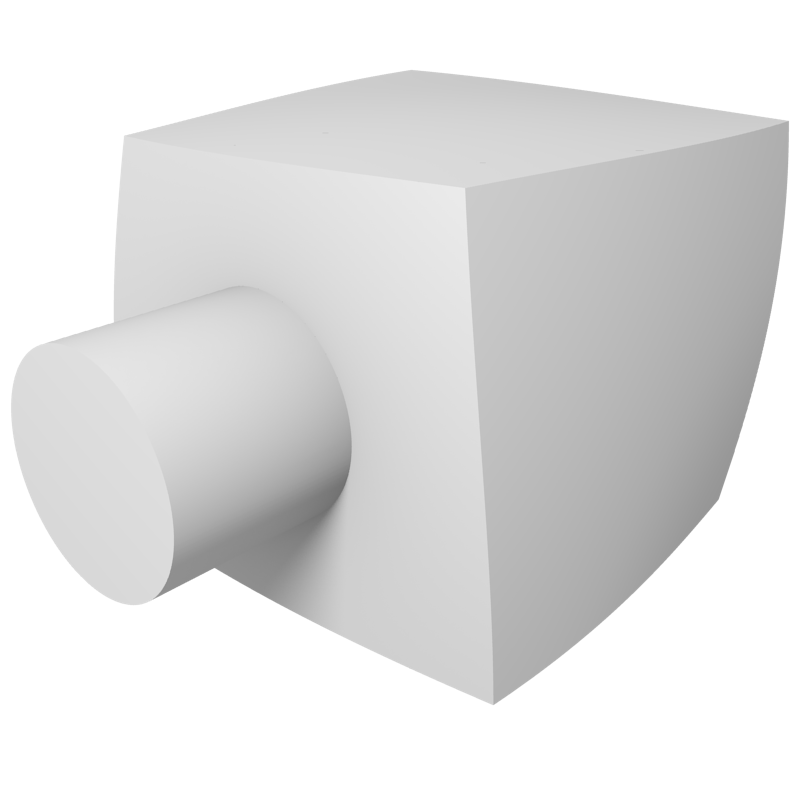
\includegraphics[width=\imagewidth]{piecewise_smooth_surface/surface}};
	%%% HIDDEN EDGES
	\node[img] at (0,0) {\includegraphics[width=\imagewidth]{piecewise_smooth_surface/edges_hidden}};
	%%% HIDDEN CORNERS
	\DTLforeach*{dbcorners}{\locx=x, \locy=y, \loca=a}{%
		\ifnum \loca = 0
			\fill[black] (\locx,\locy) circle (1.0pt);
		\fi
	}%
	%%% SURFACE (semi-transparent to mask hidden edges & corners)
	{\transparent{0.75}
		\node[img] at (0,0) {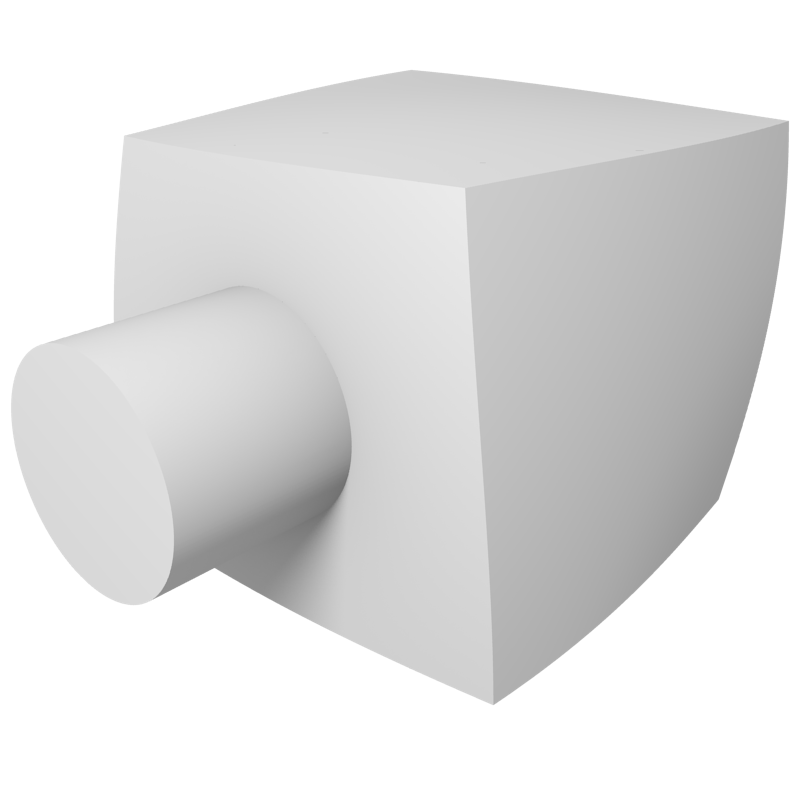
\includegraphics[width=\imagewidth]{piecewise_smooth_surface/surface}};
	}%
	%%% VISIBLE EDGES
	\node[img] at (0,0) {\includegraphics[width=\imagewidth]{piecewise_smooth_surface/edges_visible}};
	%%% VISIBLE CORNERS
	\DTLforeach*{dbcorners}{\locx=x, \locy=y, \loca=a}{%
		\ifnum \loca = 1
			\fill[black] (\locx,\locy) circle (1.2pt);
		\fi
	}%
	%
	%%% ANOTATIONS
	\DTLassign{dbcorners}{6}{\locxa=x,\locya=y,\loca=a}% 	
	\DTLassign{dbcorners}{4}{\locxb=x,\locyb=y,\loca=a}% 
	\DTLassign{dbcorners}{1}{\locxc=x,\locyc=y,\loca=a}% 
	%\node[anchor=west] (anotSingPts) at (\locxb,{0.5*(\locya + \locyb)}) {points singuliers};
	\node[anchor=east] (anotSingPts) at (1.2,0.2) {coins};
	\draw[anot] (anotSingPts) to [bend left=10] (\locxa, \locya);
	\draw[anot] (anotSingPts) to [bend right=20] (\locxb, \locyb);
	\draw[anot] (anotSingPts) to [bend right=10] (\locxc, \locyc);
	%
	\DTLassign{dbedgemidp}{19}{\locxa=x,\locya=y,\loca=a}% 	
	\DTLassign{dbedgemidp}{7}{\locxb=x,\locyb=y,\loca=a}% 
	\DTLassign{dbedgemidp}{14}{\locxc=x,\locyc=y,\loca=a}% 
	\node[anchor=west] (anotSingCurv) at (-0.2,0.9) {crêtes};
	\draw[anot] (anotSingCurv) to [bend right=10] (\locxa, \locya);
	\draw[anot] (anotSingCurv) to [bend right=40] (\locxb, \locyb);
	\draw[anot] (anotSingCurv.east) to [bend left=10] (\locxc, \locyc);
\end{tikzpicture}
\DTLgdeletedb{dbcorners}%
\DTLgdeletedb{dbedgemidp}%

	\caption{Surface régulière \piecewise\ dont les courbes et points singuliers sont mis en évidence.}
	\label{fig:piecewise_smooth_surface_decomposition}
\end{figure}

%La frontière $\boundary{\Omega}$ du solide $\Omega$ est une surface de continuité $\contgeom{1}$ (\ie possède une direction normale continue) \piecewise. 
%Les singularités géométriques de $\boundary{\Omega}$ peuvent être de dimension 1 (courbes) ou 0 (points).
%Les courbes singulières de $\boundary{\Omega}$ sont elle-mêmes des variétés différentielles de continuité $\contgeom{1}$ (\ie possède une direction tangente continue) excepté aux points singuliers.

\subsection{Représentation par les frontières (\brep)}
%Origine, utilisation, concept, définitions formelles des entités, lien avec la décomposition d'une surface $\contgeom{1}$ \piecewise, (géométrie différentielle des courbes et surfaces paramétriques), structures de données (DCEL)
La \textit{représentation par les frontières} (ou \brep\ pour \anglais{Boundary Representation}) est un formalisme très répandu dans le domaine de la Conception Assistée par Ordinateur (CAO) \textit{(développer \ldots)}.
Elle consiste à décrire un solide $\Omega$ à l'aide d'une décomposition cellulaire de la surface $\Sigma$ qui matérialise sa frontière. 
Cette décomposition --- illustrée sur la \autoref{fig:BRep} --- est constituée de \textit{faces}, d'\textit{arêtes} et de \textit{sommets} dont on donne une définition dans les paragraphes suivants. 

\begin{figure}
	\centering
	\setlength{\imagewidth}{80mm}%
\setlength{\imageheight}{\imagewidth}%
\DTLsetseparator{,}%
\DTLloaddb[noheader,keys={x,y,a}]{dbverts}{figures/data/BRep/verts_xya.dat}%
\begin{tikzpicture}[%
	x=\imagewidth, y=\imageheight,
	img/.style={anchor=south west, inner sep=0}]
	%%%%%%%%%%%%%%%% SHELL %%%%%%%%%%%%%%%%
	%%% FACES
	\node[img] at (0,0) {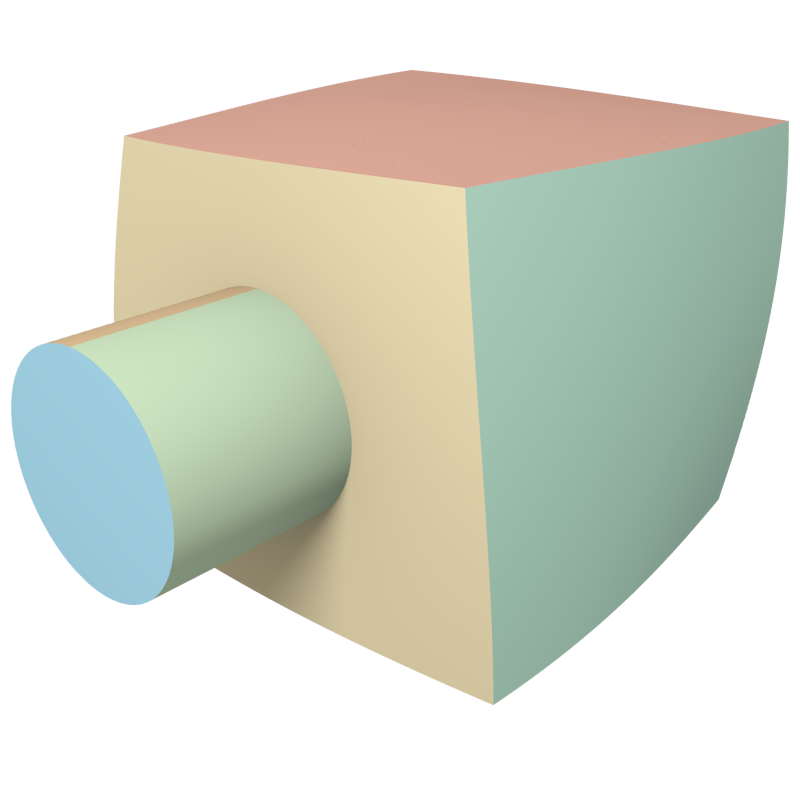
\includegraphics[width=\imagewidth]{BRep/shell}};
	%%% HIDDEN EDGES
	\node[img] at (0,0) {\includegraphics[width=\imagewidth]{BRep/edges_hidden}};
	%%% HIDDEN VERTICES
	\DTLforeach*{dbverts}{\locx=x, \locy=y, \loca=a}{%
		\ifnum \loca = 0
			\fill[black] (\locx,\locy) circle (1.0pt);
		\fi
	}%
	%%% FACES (semi-transparent to mask hidden edges & verts)
	{\transparent{0.75}
		\node[img] at (0,0) {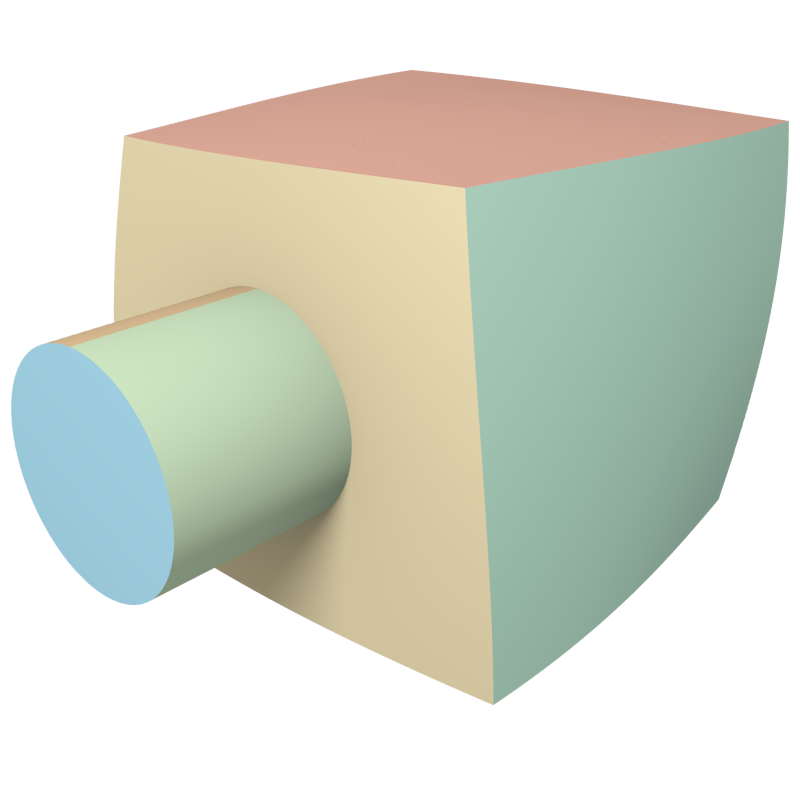
\includegraphics[width=\imagewidth]{BRep/shell}};
	}%
	%%% VISIBLE EDGES
	\node[img] at (0,0) {\includegraphics[width=\imagewidth]{BRep/edges_visible}};
	%%% VISIBLE VERTICES
	\DTLforeach*{dbverts}{\locx=x, \locy=y, \loca=a}{%
		\ifnum \loca = 1
			\fill[black] (\locx,\locy) circle (1.0pt);
		\fi
	}%
\end{tikzpicture}
\DTLgdeletedb{dbverts}%
%%%%%%%%%%%%%%%%%%%%%%%%%%%%%%%%%%%%%%
%
%%%%%%%%%%%%%%%% FACES %%%%%%%%%%%%%%%%
\def\imfacew{44mm}
\def\ngriduv{6}
\def\vertsep{0.05}
\def\edglabsepuv{0.17}
\def\wirlabsepuv{0.18}
\def\edglabsepxyz{0.06}
\def\iniwclr{0.3}
\def\decwclr{0.3}%{0.2}
\def\uvscale{0.34}
\def\uvyshift{-0.7}
\pgfmathsetmacro\sepyshift{0.5 * (\uvyshift+\uvscale)}%
%
\begin{tikzpicture}[%
	x = \imfacew, y = \imfacew,
	gridtick/.style={red, fill=white, font=\tiny, inner sep=0.5pt},
	img/.style={anchor=south west, inner sep=0},
	label/.style={inner sep=1pt, font=\scriptsize},
	uvgrid/.style={black!10!white},
	curv/.style={line width=0.8pt, line cap=round},
	spacelabel/.style={anchor=north, rotate=90, inner sep=0, font=\bfseries},
	]
	\foreach \jfa/\ifa in {-1/007, 0/008, 1/002}{%
		\figbrepface{\ifa}{{1.05*\jfa - 0.5}}{{-\sepyshift}}%\hfill
	}%
	\draw[very thick, gray, dashed] 
	({-0.5*\textwidth},0) -- ++ 
	(\textwidth,0);
	\node[spacelabel] (xyzspace) at 
	({-0.5*\textwidth},{-\sepyshift+0.5}) {Espace euclidien\vphantom{Espace paramétrique}};
	\node[spacelabel] (uvspace) at 
	({-0.5*\textwidth},{\sepyshift-\uvscale}) {Espace paramétrique\vphantom{Espace euclidien}};
\end{tikzpicture}

	\caption{Modèle \brep\ d'une surface régulière par morceaux.}
	\label{fig:BRep}
\end{figure}

\subsubsection{Faces}
\label{section:def_brep_faces}
Une face du modèle \brep\ est une variété de dimension 2 connexe délimitée par des arêtes et des sommets. 
Géométriquement, une face $\brepface$ est décrite par un carreau paramétrique restreint.
La topologie des courbes de restriction du domaine paramétrique est décrite à l'aide de \textit{contours} (un par composante connexe du bord de $\brepface$). 
Une face possède ainsi un contour extérieur $\brepwire^{\mathrm{ext}}$ et, éventuellement un ou plusieurs contours intérieurs $\brepwire^{\mathrm{int},i}$ si celle-ci comporte des \guillemets{trous}.
Les faces, qui sont quasi-disjointes deux-à-deux (\ie ne s'intersectent qu'en des arêtes ou des sommets du modèle \brep), sont regroupées en \textit{coquilles}, qui représentent chacune une composante connexe de $\Sigma$. 


\subsubsection{Arêtes}
\label{section:def_brep_edges}
Une arête du modèle \brep\ est une variété de dimension 1 connexe délimitée par des sommets.
Puisque $\Sigma$ est une variété sans bord, chaque arête du modèle \brep\ est incidente à exactement deux faces $\brepface_1$ et $\brepface_2$. 
Géométriquement, l'arête $\brepedge$ est représentée par une branche de la courbe d'intersection entre les carreaux $\Sigma_1$ et $\Sigma_2$ qui décrivent respectivement $\brepface_1$ et $\brepface_2$. 
Cette courbe peut également être représentée par sa trace dans l'espace paramétrique de chaque carreau. 
On peut donc la représenter à l'aide des trois courbes paramétriques $\bg$, $\bp_1$ et $\bp_2$ telles que
\begin{equation}
	\bg = \bs_1 \circ \bp_1 = \bs_2 \circ \bp_2.
\end{equation}

\begin{figure}
	\centering
	\setlength{\imagewidth}{67.5mm}
\setlength{\imageheight}{\imagewidth * \real{0.75}}
%
\def\uvscale{0.28}
\def\fracaxeoffset{0.0}
\def\distanceaxe{0.1}
\def\psisep{-0.42}
%
\DTLsetseparator{,}%
\DTLloaddb[noheader,keys={x,y}]{dbpoint}{figures/data/simple_intersection/point.dat}%
\DTLassign{dbpoint}{1}{\xloc=x, \yloc=y}% 
%
\begin{tikzpicture}[
	x=\imagewidth, y=\imageheight, 
	axe/.style={-stealth, line width=0.5pt},
	uvdomain/.style={thin}, 
	image/.style={anchor=south west, inner sep=0},
	curve/.style={thick, line cap=round},
	label/.style={font=\normalsize},
	axelabel/.style={font=\small},
	axeuvlabel/.style={axelabel, inner sep=0},
	point/.style={fill=black, circle, scale=0.3},
	map/.style={-{Classical TikZ Rightarrow[length=4pt,width=4pt]}}]
	%
	\node[image] (img) at (0,0) {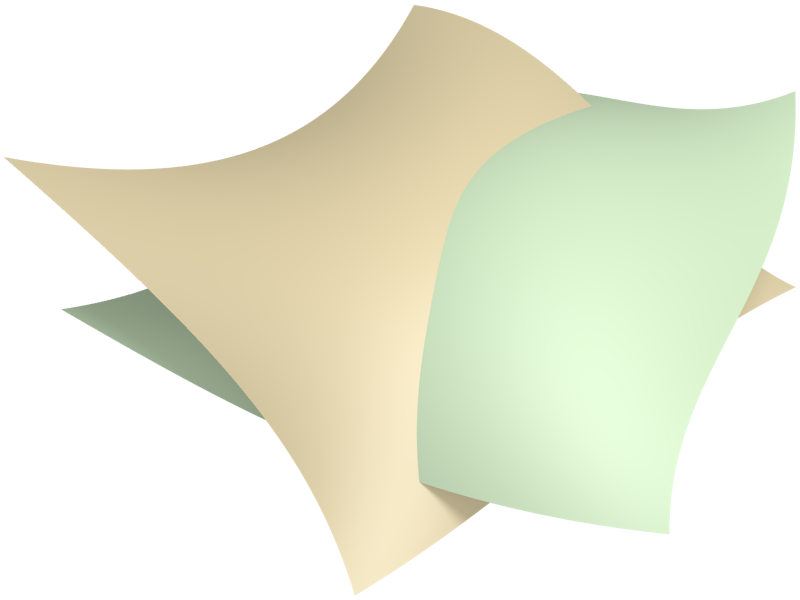
\includegraphics[width=\imagewidth]{figures/images/simple_intersection/surfaces}};
	\node[image] (img) at (0,0) {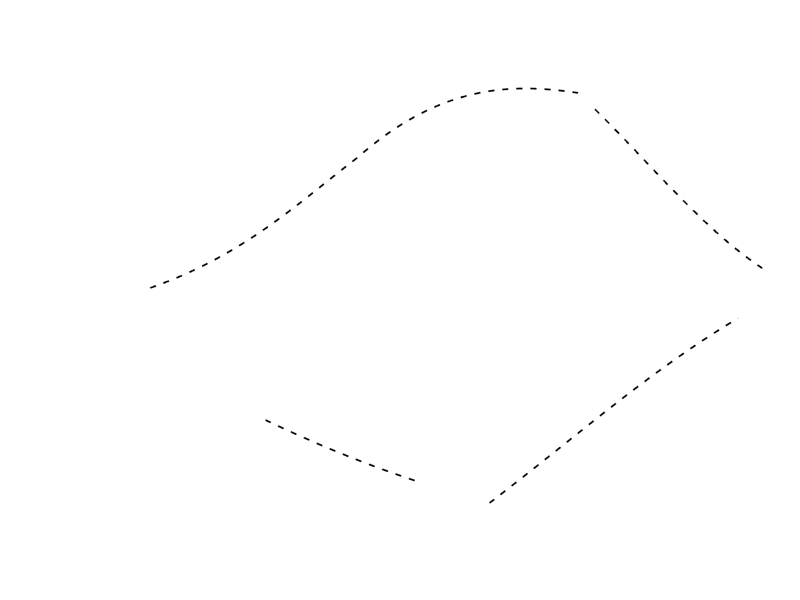
\includegraphics[width=\imagewidth]{figures/images/simple_intersection/borders_hidden}};
	{\transparent{0.75}%
		\node[image] (img) at (0,0) {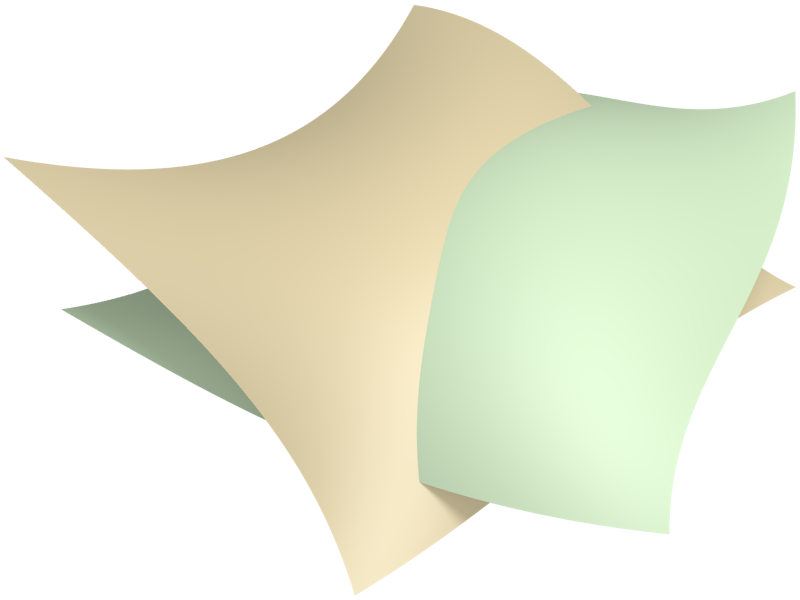
\includegraphics[width=\imagewidth]{figures/images/simple_intersection/surfaces}};
	}%
	\node[image] (img) at (0,0) {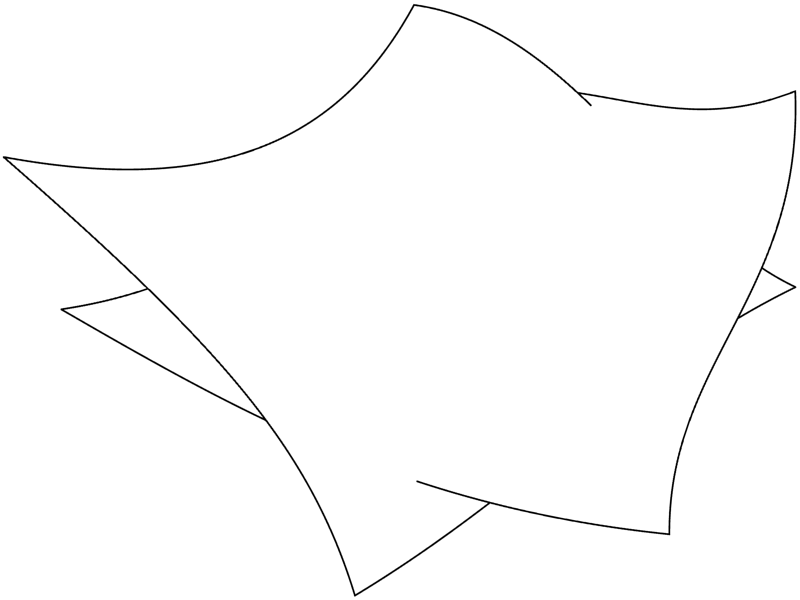
\includegraphics[width=\imagewidth]{figures/images/simple_intersection/borders_visible}};
	\draw[curve] plot file {figures/data/simple_intersection/curve_xy.dat};
	\node[point] (xyz) at (\xloc, \yloc) {};
	\node[label, anchor=east] at (\xloc, \yloc) {$\bg(w)$};
	%
	\node[label] at (0.56, 0.91) {$\Sigma_1$};
	\node[label] at (0.93, 0.75) {$\Sigma_2$};
	%
%	\foreach \igrid in  {0,0.1,...,1.01}{
%		\draw[red, thin] (0,\igrid) -- (1,\igrid)
%		                 (\igrid,0) -- (\igrid,1);
%	}
	% 
	% trièdre
	\def\scaletriedre{0.8}
	\coordinate (o) at (0.13209545612335205 , 0.14773482084274292);
	\coordinate (x) at (0.23464959859848022 , 0.02938912808895111);
	\coordinate (y) at (0.26169726252555847 , 0.2535654902458191);
	\coordinate (z) at (0.1061694324016571 , 0.31903284788131714);
	\draw[axe] (o) -- ($(o)!\scaletriedre!(x)$) node[axelabel, anchor=west] {$x$};
	\draw[axe] (o) -- ($(o)!\scaletriedre!(y)$) node[axelabel, anchor=west] {$y$};
	\draw[axe] (o) -- ($(o)!\scaletriedre!(z)$) node[axelabel, anchor=south] {$z$};
	%
	\begin{scope}[scale=\uvscale, x=\imageheight, y=\imageheight, shift={(img.west)}]
		\begin{scope}[shift={(-1.5,0.7)}]
			\DTLloaddb[noheader,keys={r,g,b}]{dbsurfacecolor}{figures/data/BRep/faces/facecolor_002.dat}%
			\DTLassign{dbsurfacecolor}{1}{\rfai=r,\gfai=g,\bfai=b}% 
			\definecolor{surfacecolor}{RGB}{\rfai,\gfai,\bfai}
			\draw[uvdomain, fill=surfacecolor] (-1,-1) -- (1,-1) -- (1,1) -- (-1,1) -- cycle;
			\DTLgdeletedb{dbsurfacecolor}
			%
			\draw[curve] plot file {/d/bandrieu/GitHub/FFTsurf/test/demo_intersection/simple/curve_uv1.dat};
			%
			\DTLassign{dbpoint}{2}{\uloc=x, \vloc=y}% 
			\DTLassign{dbpoint}{3}{\duloc=x, \dvloc=y}% 
			\node[point] (uv1) at (\uloc, \vloc) {};
			%\node[label] at ({\uloc + \psisep*\duloc}, {\vloc + \psisep*\dvloc}) {$\bp_1(w)$};
			\node[label, anchor=north east, inner sep=0] at (\uloc, \vloc) {$\bp_1(w)$};
			% Axes
			\coordinate (o) at ({-1-\distanceaxe},{-1-\distanceaxe});
			\draw[axe] (o) -- ++ ({\fracaxeoffset+\distanceaxe+0.5},0) node [axeuvlabel, anchor=north west] {$u_1$};
			\draw[axe] (o) -- ++ (0,{\fracaxeoffset+\distanceaxe+0.5}) node [axeuvlabel, anchor=south east] {$v_1$};
		\end{scope}
	\end{scope}
	%
	\begin{scope}[scale=\uvscale, x=\imageheight, y=\imageheight, shift={(img.east)}]
		\begin{scope}[shift={(1.6,-0.9)}]
			\DTLloaddb[noheader,keys={r,g,b}]{dbsurfacecolor}{figures/data/BRep/faces/facecolor_008.dat}%
			\DTLassign{dbsurfacecolor}{1}{\rfai=r,\gfai=g,\bfai=b}% 
			\definecolor{surfacecolor}{RGB}{\rfai,\gfai,\bfai}
			\draw[uvdomain, fill=surfacecolor] (-1,-1) -- (1,-1) -- (1,1) -- (-1,1) -- cycle;
			\DTLgdeletedb{dbsurfacecolor}
			%
			\draw[curve] plot file {/d/bandrieu/GitHub/FFTsurf/test/demo_intersection/simple/curve_uv2.dat};
			%
			\DTLassign{dbpoint}{4}{\uloc=x, \vloc=y}% 
			\DTLassign{dbpoint}{5}{\duloc=x, \dvloc=y}% 
			\node[point] (uv2) at (\uloc, \vloc) {};
			%\node[label] at ({\uloc + \psisep*\duloc}, {\vloc + \psisep*\dvloc}) {$\bp_2(w)$};
			\node[label, anchor=north east, inner sep=0] at (\uloc, \vloc) {$\bp_2(w)$};
			% Axes
			\coordinate (o) at ({-1-\distanceaxe},{-1-\distanceaxe});
			\draw[axe] (o) -- ++ ({\fracaxeoffset+\distanceaxe+0.5},0) node [axeuvlabel, anchor=north west] {$u_2$};
			\draw[axe] (o) -- ++ (0,{\fracaxeoffset+\distanceaxe+0.5}) node [axeuvlabel, anchor=south east] {$v_2$};
		\end{scope}
	\end{scope}
	%
	% mappings
	\draw [map, shorten <= 5mm, shorten >= 5mm] (uv1) to [bend left =40] node [label, anchor=south west] {$\bs_1$} (xyz);
	\draw [map, shorten <= 5mm, shorten >= 5mm] (uv2) to [bend right=40] node [label, anchor=south west] {$\bs_2$} (xyz);
	%
%	\draw[red, thin, dashed] (current bounding box.south west) rectangle (current bounding box.north east);
\end{tikzpicture}
\DTLgdeletedb{dbpoint}
	\caption{Description géométrique d'une arête \brep.}
\end{figure}

Les arêtes, qui sont quasi-disjointes deux-à-deux (\ie ne s'intersectent qu'en des sommets du modèle \brep), sont regroupées pour former les contours des faces. 
Puisque ces derniers sont orientés, chaque arête $\brepedge$ est formée de deux \textit{co-arêtes} jumelles $\brepedge^1$ et $\brepedge^2$, chacune associée à une face incidente à $\brepedge$. 
Chaque co-arête possède une orientation, conforme à celle du contour qui la contient.


\subsubsection{Sommets}
\label{section:def_brep_vertices}
Un sommet du modèle \brep\ matérialise l'intersection de deux arêtes et a pour support géométrique un point de $\reals^3$.

\subsubsection{Structure de données}
\begin{enumerate}
	\item séparation entre topologie (structure) / géométrie (forme)
	\item connectivité entre les entités capturée à l'aide d'une structure de graphe (homéomorphe à un polyèdre)
	\item structure de données adaptée $\to$ \anglais{Doubly Connected Edge List} (DCEL) (\anglais{Halfedges}) \textit{(donner réfs.)}
\end{enumerate}

La \autoref{fig:BRep_hierarchy} présente un diagramme de la hiérarchie des entités qui constituent le modèle \brep.
\begin{figure}
	\centering
	\colorlet{topo_color}{mycolor_5}
\colorlet{orient_color}{topo_color!60!mycolor_2}
\colorlet{group_color}{topo_color!40!mycolor_3}
\colorlet{geom_color}{mycolor_1}%{mycolor_3}
\def\bigsep{5mm}
\def\smallsep{2.5mm}
\pgfdeclarelayer{bg}    % declare background layer
\pgfsetlayers{bg,main}  % set the order of the layers (main is the standard layer)
\begin{tikzpicture}[
	x = 30mm,
	y = 9.75mm,
	arrow/.style={thick, -stealth', shorten <= 2pt, shorten >= 2pt},
	bounded/.style={arrow, dash pattern=on 4pt off 2pt},
	described/.style={arrow},
	composed/.style={arrow, dash pattern=on 1.5pt off 1.5pt},
	box/.style={rectangle, rounded corners=0.8ex},
	number/.style={font=\footnotesize},
	topo/.style={fill=topo_color!33!white},
	geom/.style={fill=geom_color!33!white},
	orient/.style={fill=orient_color!33!white},
	group/.style={fill=group_color!33!white},
	type/.style={font=\bfseries},%, anchor=east},
	label/.style={anchor=west, inner sep=2pt, font=\scriptsize},
	class/.style={dotted, thick, line cap=round},
	bigclass/.style={class, rounded corners=\bigsep, dash pattern=on 0.8pt off 3.2pt},
	smallclass/.style={class, rounded corners=\smallsep, dash pattern=on 0.3pt off 2.8pt},
	]
	% entités topologiques
	\node[box, topo] at (-1,1) (volume) {Solide};
	\node[box, topo] at (0,1) (face) {Face};
	\node[box, topo] at (1,1) (edge) {Arête};
	\node[box, topo] at (2,1) (vertex) {Sommet};
	% entités de groupement
	\node[box, group] at (-1,3) (shell) {Coquille};
	\node[box, group] at (0,3) (wire) {Contour};
	% entités d'orientation
	\node[box, orient] at (1,3) (halfedge) {Co-arête};
	% entités géométriques
	\node[box, geom] at (0,-1) (surface) {Surface};
	\node[box, geom] at (1,-1) (curve) {Courbe};
	\node[box, geom] at (2,-1) (point) {Point};
	%
	% relations "décrit par"
	\draw[described] (face) -- (surface);
	\draw[described] (edge) -- (curve);
	\draw[described] (vertex) -- (point);
	% relations "délimité par"
	\draw[bounded] (volume) -- 
		node[number,left]{$1+n_{\mathrm{s}}^{\mathrm{int}}$} 
		(shell);
	\draw[bounded] (face) -- 
		node[number,right]{$1+n_{\mathrm{w}}^{\mathrm{int}}$} 
		(wire);
	\draw[bounded] (edge) -- node[number,above]{$2$} (vertex);
	% relations "composé de"
	\draw[composed] (shell) -- node[number,above right]{$n$} (face);
	\draw[composed] (wire) -- node[number,above]{$n$} (halfedge);
	\draw[composed] (edge) -- node[number,right]{$2$} (halfedge);
	%
	% noms de classes
	\gettikzxy{(current bounding box.east)}{\xbbE}{\ybbE}%
	\node[type, geom_color!90!gray] (geomet) at (-1,-1) {Géométrie};
	\node[type, anchor=east, orient_color!90!gray] (orientation) at ({\xbbE-0.5*\smallsep},3) {Orientation};
	\gettikzxy{(halfedge.east)}{\xhE}{\yhE}%
	\gettikzxy{(orientation.west)}{\xoW}{\yoW}%
	\gettikzxy{(shell.west)}{\xsW}{\ysW}%
	\node[type, anchor=east, group_color!90!gray] (grouping) at ({\xsW-\xoW+\xhE},3) {Groupement};
	\gettikzxy{(grouping.west)}{\xgrW}{\ygrW}%
	\gettikzxy{(grouping.south)}{\xgrS}{\ygrS}%
	\gettikzxy{(volume.south)}{\xvS}{\yvS}%
	\node[type, anchor=west, topo_color!90!gray] (topology) at (\xgrW,{0.5*(\ygrS-\smallsep + \yvS-\bigsep)}) {Topologie};
	%
	% classes
	\gettikzxy{(vertex.south east)}{\xtSE}{\ytSE}%
	\gettikzxy{(shell.north)}{\xtN}{\ytN}%
	\gettikzxy{(grouping.west)}{\xtW}{\ytW}%
	\gettikzxy{(geomet.west)}{\xgeW}{\ygeW}%
	\gettikzxy{(topology.north)}{\xtM}{\tmp}%
	\gettikzxy{(grouping.south)}{\tmp}{\ytM}%
	\gettikzxy{(halfedge.south west)}{\xoSW}{\yoSW}%
	\gettikzxy{(halfedge.north)}{\xoN}{\yoN}%
	\gettikzxy{(orientation.north east)}{\xoNE}{\yoNE}%
	\gettikzxy{(grouping.south west)}{\xgrSW}{\ygrSW}%
	\gettikzxy{(wire.south)}{\xgrS}{\ygrS}%
	\gettikzxy{(wire.north east)}{\xgrNE}{\ygrNE}%
	\gettikzxy{(surface.south)}{\xgeS}{\ygeS}%
	\gettikzxy{(surface.north)}{\xgeN}{\ygeN}%
	\begin{pgfonlayer}{bg}    % select the background layer
		\draw[bigclass, topo_color, fill=topo_color!8!white] 
		({\xtSE+\bigsep},{\ytSE-\bigsep}) --
		({\xtSE+\bigsep},{\ytN+\bigsep}) --
		({\xtW-\bigsep},{\ytN+\bigsep}) --
		({\xtW-\bigsep},{\ytSE-\bigsep}) -- cycle;
		%
		\draw[smallclass, orient_color, fill=orient_color!8!white] 
		({\xoSW-\smallsep},{\yoSW-\smallsep}) -- 
		({\xoNE+\smallsep},{\yoSW-\smallsep}) -- 
		({\xoNE+\smallsep},{\yoN+\smallsep}) -- 
		({\xoSW -\smallsep},{\yoN+\smallsep}) -- cycle;
		%
		\draw[smallclass, group_color, fill=group_color!8!white] 
		({\xgrSW-\smallsep},{\ygrS-\smallsep}) -- 
		({\xgrNE+\smallsep},{\ygrS-\smallsep}) -- 
		({\xgrNE+\smallsep},{\ygrNE+\smallsep}) -- 
		({\xgrSW -\smallsep},{\ygrNE+\smallsep}) -- cycle;
		%
		\draw[bigclass, geom_color, fill=geom_color!8!white]
		({\xgeW-\bigsep},{\ygeS-\bigsep}) -- 
		({\xtSE+\bigsep},{\ygeS-\bigsep}) -- 
		({\xtSE+\bigsep},{\ygeN+\bigsep}) -- 
		({\xgeW-\bigsep},{\ygeN+\bigsep}) -- cycle;
	\end{pgfonlayer}
	% légende des relations
	\coordinate (lgd) at ({\xtW-\bigsep+2pt},{0.5*(\ygeS+\ygeN)});
	\foreach \i in {0,1,2}{
		\coordinate (L\i) at ([yshift={-(\i-1)*2.8ex}]lgd);
		\coordinate (R\i) at ([xshift=7.5mm]L\i);
	}
	\draw[described] (L0) -- (R0) node[label] (lbl0) {décrit par};
	\draw[bounded]   (L1) -- (R1) node[label] (lbl1) {délimité par};
	\draw[composed]  (L2) -- (R2) node[label] (lbl2) {composé de};
	\node[draw=black!25,
	inner sep=2pt,
	rounded corners=\smallsep,
	fit={(L0) (lbl0) (lbl1) (lbl2)}] {};
\end{tikzpicture}
	\caption{Hiérarchie des éléments constituant un modèle \brep.}
	\label{fig:BRep_hierarchy}
\end{figure}


\subsubsection{Représentation de surfaces régulières par morceaux}
Le formalisme de la représentation par les frontières est particulièrement adapté pour décrire des surfaces régulières par morceaux. 
En effet, 
\begin{itemize}
	\item l'ensemble des points singuliers de $\Sigma$ est un sous-ensemble des sommets de son modèle \brep\ ;
	\item l'ensemble des courbes singulières de $\Sigma$ est un sous-ensemble des arêtes de son modèle \brep\ ;
	\item les nappes régulières de $\Sigma$ sont formées par la réunion des faces de son modèle \brep.
%	\item chaque arête \brep\ vive est contenue dans une courbe singulière
\end{itemize}











\section{Formulation lagrangienne du problème de propagation d'interface}
On considère une interface $\Sigma$ entre deux milieux distincts (\eg un solide et un fluide).
Dans cette thèse, on se concentre sur des problèmes en trois dimensions. 
$\Sigma$ représente donc une surface (\ie une variété de dimension 2) que l’on supposera orientable et fermée (\ie sans bord).
De cette manière, l'interface sépare un domaine \textit{intérieur} $\Omega$ --- que l'on supposera ouvert --- et un domaine \textit{extérieur} $\complement{\Omega} = \reals^3 \setminus \Omega$.
\par
%[EDP avec vecteur vitesse ou vitesse normale, problème de définition au niveau des courbes singulières et points irréguliers]
%\par\bigskip
Le problème que l'on cherche à résoudre consiste à déterminer l’évolution au cours du temps de l'interface $\Sigma$ étant données sa position actuelle ainsi que sa vitesse de propagation.
Dans la formulation lagrangienne traditionnelle, ce problème est exprimé sous la forme d'une équation aux dérivées partielles (EDP) pour le vecteur position $\bx$ d'un point de l'interface.
L'équation décrivant la propagation suivant un champ de vecteur vitesse $\vrm{u} : \Sigma \times \reals \to \reals^3$ est
\begin{equation}
	\frac{\partial \bx}{\partial t} = \vrm{u}(\bx,t).
	\label{eq:lagrange_vecteur_vitesse}
\end{equation}
On peut également considérer que chaque point de $\Sigma$ se déplace le long de la direction normale à l'interface suivant un champ de vitesse normale $\nu : \Sigma \times \reals \to \reals$. 
L'équation décrivant la propagation est alors
\begin{equation}
	\frac{\partial \bx}{\partial t} = \nu(\bx,t) \unv(\bx,t),
	\label{eq:lagrange_vitesse_normale}
\end{equation}
où $\unv(\bx,t)$ désigne la direction normale à $\Sigma$ en $\bx$ à l'instant $t$, pointant vers l'extérieur de $\Omega$.
\par\bigskip
En principe, les formulations \eqref{eq:lagrange_vecteur_vitesse} et \eqref{eq:lagrange_vitesse_normale} sont équivalentes puisque la composante tangentielle du vecteur vitesse n'affecte pas la forme de l'interface. 
\par\bigskip
La formulation lagrangienne ne permet d'obtenir une solution au problème de propagation d'interface que dans le cas où cette dernière est \textit{globalement} régulière et le reste tout au long de sa propagation. 
En effet, puisque la direction normale $\unv$ n'est pas définie au niveau des courbes et points singuliers de $\Sigma$, le déplacement de ces points est ambigu. 
On peut notamment distinguer deux cas \cite{jiao2007}.
\par
Premièrement, si l'interface subit un mouvement d'advection (comme le transport d'un fluide ou encore la déformation d'un solide sous l'effet de contraintes mécaniques) alors ses singularités géométriques sont préservées au cours de la propagation.
\par
En revanche, si l'interface se propage à la manière d'un front d'onde (comme la progression d'une flamme, d'un dépôt de matière ou encore l'ablation d'un solide) alors les singularités sont soit préservées soit régularisées, suivant la convexité locale de l'interface.
C'est essentiellement sur ce deuxième type de propagation que l'on se concentre dans cette thèse.
\par\bigskip
Puisque l'on s'intéresse ici à la propagation d'interfaces régulières seulement \piecewise, il est nécessaire d'obtenir une meilleure formulation du problème qui s'affranchisse des ambiguïtés ainsi mises en évidence. 
Plutôt que de poser le problème sous la forme d'une équation différentielle, cette nouvelle formulation se présente comme une construction géométrique.

\section{Principe de Huygens avec condition d'entropie}
\label{section:principe_huygens}
\def\p{\vit{p}}
\def\q{\vit{q}}
%
%[Histoire, formulation, notion d'enveloppe de sphères/boules, construction géométrique au lieu de EDP, équations définissant l'EdS propre à 1/2 paramètre(s), différence d'ordre 2 avec transport suivant la normale, définitions implicites (\cf notes Huygens)]
%\par\bigskip
Alors qu'il développait un modèle ondulatoire de la propagation de la lumière, Christiaan Huygens proposa le principe suivant : chaque point de l'espace atteint par une onde lumineuse se comporte comme la source d'une ondelette secondaire émise dans toutes les directions. 
Si le milieu de propagation est homogène et isotrope alors les ondelettes sont sphériques. 
Le front d'onde, qui se propage ainsi de proche en proche, est alors formé par l'\textit{enveloppe} de ces ondelettes, \ie la surface qui est tangente à chacune d'elles et dont chaque point est un point de tangence avec une ondelette.
\par
Le principe de Huygens permet de décrire de nombreux phénomènes analogues à la propagation d'une onde dans un milieu tels que la progression d'une flamme. 
\textit{(développer \ldots)}

\par\bigskip
\begin{enumerate}
	\item distinguer propagation d'une onde et d'une interface entre deux milieux matériels (l'une peut s'auto-intersecter, l'autre non) $\to$ condition d'entropie
	%\item formaliser la notion d'enveloppe des sphères $\EdS{\Sigma}{\rho}$ (surface tangente à toutes les sphères et en tout point tangente à une sphère) $\to$ système d'équations avec $\implicitsphere_{\rho} : (\bx,\p) \mapsto \normtwo{\bx - \p}^2 - \rho^2(\p)$
	%\item formaliser la notion d'enveloppe des boules $\EdB{\Sigma}{\rho} := \boundary{\left\{\Omega \cup \sphere[\Sigma][\rho]\right\}}$
	\item formaliser la notion d'enveloppe des sphères (EdS) $\EdS{H \subseteq \Sigma}{\rho}$ (surface tangente à toutes les sphères et en tout point tangente à une sphère)
	%\item formaliser la notion d'enveloppe des boules $\EdB{\Sigma}{\rho} := \boundary{\left\{\Omega \cup \sphere[\Sigma][\rho]\right\}}$
	\item formaliser la notion d'enveloppe des boules (EdB) $\EdB{H \subseteq \Sigma}{\rho} := \boundary{ \left( \ball{H}{\rho} \right) }$
	\item si $H \subseteq \Sigma$ est une variété sans bord alors $\EdB{H}{\rho}  = \EdBplus{H}{\rho} \cup \EdBmoins{H}{\rho}$ où $\EdBplus{H}{\rho} \subset \complement{\Omega}$ et $\EdBmoins{H}{\rho} \subset \Omega$ (\textit{illustrer})
	\item donner définition implicite de l'EdB :\\
	on pose 
	\[
		\implicitsphere(\bx, \p) := \normtwo{\bx - \p}^2 - \rho(\p)^2,
	\]
	et, pour $H \subseteq \Sigma$, 
	\[
		\implicitEdB{H}(\bx) := \min_{\p \in H} \implicitsphere(\bx, \p).
	\]
	Alors,
	\[ 
		\EdB{H}{\rho} 
		= \implicitEdB{H}^{-1}(0)
		= 
		\left\{
			\bx \in \reals^3 \mid \forall \p \in H, \implicitsphere(\bx, \p) \geq 0
			\text{ et } \exists \q \in H \mid \implicitsphere(\bx, \p) = 0
		\right\}.
	\]
	\item après une propagation à vitesse normale $\nu$ constante pendant un intervalle de temps $\tau$ tel que $\nu \tau = \rho$, la nouvelle interface est $\EdBplus{\Sigma}{\rho}$
	\item à condition que $\rho$ soit suffisamment régulière (continuité à déterminer), $\EdB{\Sigma}{\rho} \subseteq \EdS{\Sigma}{\rho}$
	\item si $\EdS{\Sigma}{\rho}$ ne présente pas d'auto-intersections alors $\EdB{\Sigma}{\rho} = \EdS{\Sigma}{\rho}$
\end{enumerate}


\setlength{\imagewidth}{50mm}
\setlength{\imageheight}{\imagewidth}
\begin{figure}
	\centering
	%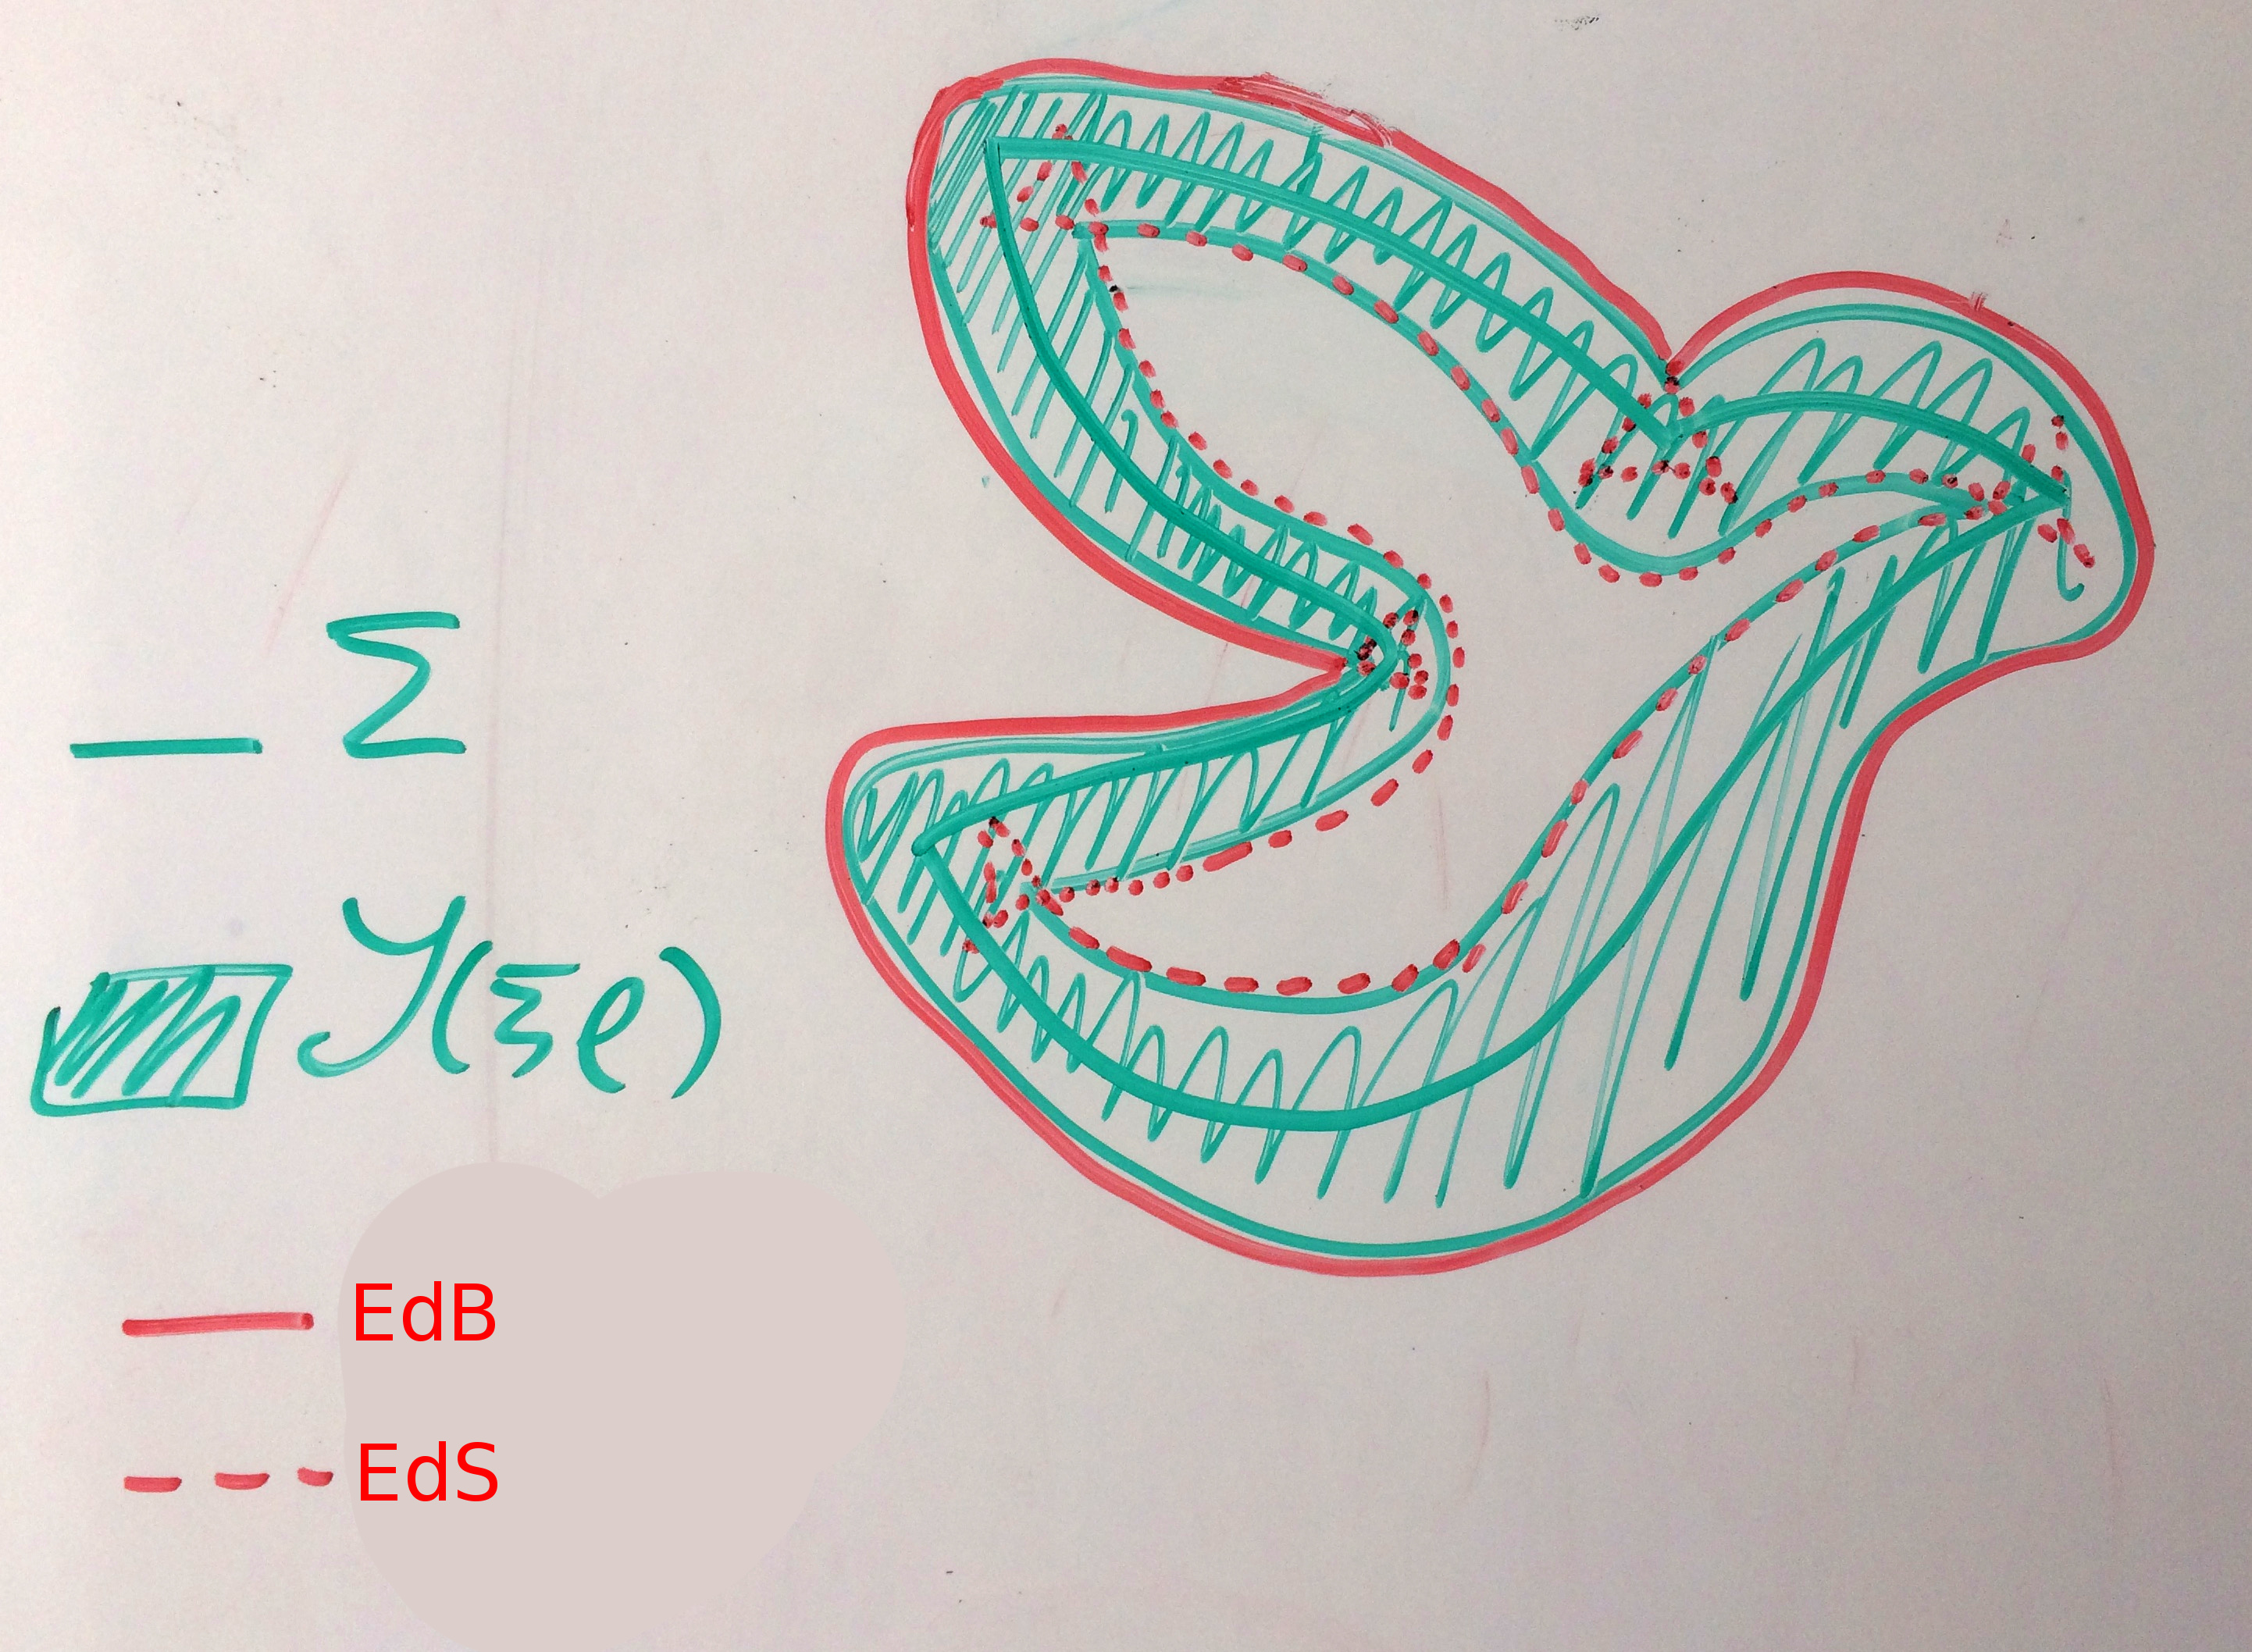
\includegraphics[width=10cm]{EdS_EdB.JPG}
	\begin{tikzpicture}[
		x=\imagewidth, y=\imageheight,
		solide/.style={fill=yellow},
		EdS/.style={densely dotted},
		EdB/.style={},
		plus/.style={red, thick},
		moins/.style={blue},
	]
		\draw[solide]
	(-0.06746503840974725, -0.4895808548348827) .. controls (0.3754890683456228,-0.4895808548348827) and (0.3988024423853791,-0.46626748079512637) .. (0.3988024423853791,-0.44295410675537006) --
(0.3988024423853791, -0.44295410675537006) .. controls (0.3988024423853791,-0.42431526272572534) and (0.4981464229889558,-0.3758732245150076) .. (0.5379850510539838,-0.28571429213755745) --
(0.5379850510544867, -0.28571429213793853) .. controls (0.8699302429858553,-0.18565116416061012) and (0.6967765088651833,0.14746923507300805) .. (0.9583234193395308,0.2564471144373195) --
(0.9583234193395308, 0.2564471144373195) .. controls (0.9870006267090254,0.26839595084127554) and (0.9999999999999999,0.27642532872560166) .. (0.9999999999999999,0.27932994073590234) --
(0.9999999999999999, 0.27932994073590234) .. controls (0.9368906834736912,0.2775306754796471) and (0.8184431751009927,0.2739321449671367) .. (0.8106720504210739,0.2739321449671367) --
(0.8106720504210739, 0.2739321449671367) .. controls (0.8029009257411553,0.2739321449671367) and (0.7873586763813178,0.2681038014571977) .. (0.7718164270214803,0.2564471144373195) --
(0.7718164270214803, 0.2564471144373195) .. controls (0.6581309712183425,0.17118302258496643) and (0.7263502504007378,-0.011530034438207932) .. (0.5250336663999142,-0.04221172606526177) --
(0.5250336664200125, -0.04221172607833209) .. controls (0.4953911362021426,0.05361085742211611) and (0.4470967892937609,0.1550289859297178) .. (0.3988024423853791,0.2564471144373195) --
(0.3988024423853791, 0.2564471144373195) .. controls (0.38908853653548064,0.27684631672210636) and (0.37646045893061264,0.28704591786449973) .. (0.36868933425069383,0.28704591786449973) --
(0.36868933425069383, 0.28704591786449973) .. controls (0.33921010764770126,0.28704591786309486) and (0.3097308810447087,0.28704591786169) .. (0.28025165444171607,0.287045917860285) --
(0.28025165444171607, 0.287045917860285) .. controls (0.19518025597352578,0.30684062482995533) and (0.03920279945779625,0.3163264802751997) .. (-0.005296040970397075,0.34970061059634483) --
(-0.005296040970397075, 0.34970061059634483) .. controls (-0.06746503840974725,0.39632735867585744) and (0.18121095134765347,0.4895808548348827) .. (-0.06746503840974725,0.4895808548348827) --
(-0.06746503840974725, 0.4895808548348827) .. controls (-0.316141028167148,0.4895808548348827) and (-0.06746503840974725,0.39632735867585744) .. (-0.12963403584909744,0.34970061059634483) --
(-0.12963403584909744, 0.34970061059634483) .. controls (-0.17413287627729077,0.3163264802751997) and (-0.3301103327930203,0.30684062482995533) .. (-0.4151817312612106,0.287045917860285) --
(-0.4151817312612106, 0.287045917860285) .. controls (-0.44466095786420323,0.28704591786169) and (-0.4741401844671958,0.28704591786309486) .. (-0.5036194110701884,0.28704591786449973) --
(-0.5036194110701884, 0.28704591786449973) .. controls (-0.5113905357501072,0.28704591786449973) and (-0.5240186133549751,0.27684631672210636) .. (-0.5337325192048736,0.2564471144373195) --
(-0.5337325192048736, 0.2564471144373195) .. controls (-0.5411370998372399,0.24089749510935002) and (-0.5485416804696063,0.22534787578138069) .. (-0.5558790356630344,0.20981842408509274) --
(-0.5558790114531827, 0.2098184235500931) .. controls (-0.8519596704843941,0.20973954266796285) and (-0.9999999999999999,0.20645798067563845) .. (-0.9999999999999999,0.06994012211926898) --
(-0.9999999999999999, 0.06994012211926898) .. controls (-0.9999999999999999,-0.06828492072961546) and (-0.8937637786585189,-0.19512751129191278) .. (-0.6662943175035188,-0.29933988571359427) --
(-0.6662943174455495, -0.2993398856489413) .. controls (-0.6230882896643332,-0.38079329947914053) and (-0.5337325192048736,-0.4252770686861742) .. (-0.5337325192048736,-0.44295410675537006) --
(-0.5337325192048736, -0.44295410675537006) .. controls (-0.5337325192048736,-0.46626748079512637) and (-0.5104191451651173,-0.4895808548348827) .. (-0.06746503840974725,-0.4895808548348827) --
cycle
	(-0.5883356839966504, 0.13987681371693386) .. controls (-0.6441212594821244,0.016657347260371286) and (-0.689155012803249,-0.1033365725468865) .. (-0.689155012803249,-0.20982036635780685) --
(-0.689155012803249, -0.20982036635780685) .. controls (-0.8445775064016244,-0.1398802442385379) and (-0.9067465038409747,0.0) .. (-0.9067465038409747,0.06994012211926898) --
(-0.9067465038409747, 0.06994012211926898) .. controls (-0.9067465038409747,0.13732005960362262) and (-0.7913447805045282,0.13978652771122496) .. (-0.5883356837283094,0.13987681370959412) --
cycle;
		%
		\node at (-0.06,-0.055) {$\Omega$};
		\node at (0.45,0.45) {$\complement{\Omega}$};
%		\node[above] at (-0.5,0.28) {$\Sigma$};
		%
		\draw[EdS, plus]
	(-0.06841257566169621, -0.5185952086135809) -- (-0.05508852476298517, -0.5190208405851853) -- (-0.04200982102055934, -0.5194177422388051) -- (-0.02917419081324142, -0.5197836870228345) -- (-0.016579449764495525, -0.5201168099070985) -- (-0.004223492987314413, -0.5204155935497116) -- (0.007895716030030041, -0.5206788514604755) -- (0.019780157405484236, -0.520905708797223) -- (0.03143176725360698, -0.5210955813776642) -- (0.04285245007483758, -0.5212481534353148) -- (0.054044090791478115, -0.5213633545944871) -- (0.0650085661410164, -0.5214413364865651) -- (0.07574775520127126, -0.521482449378189) -- (0.0862635488836833, -0.5214872191319371) -- (0.09655785828859673, -0.5214563247719387) -- (0.10663262186797531, -0.5213905768809631) -- (0.11648981138568029, -0.5212908970122154) -- (0.12613143670276683, -0.5211582982586762) -- (0.13555954944518764, -0.5209938670855756) -- (0.1447762456341446, -0.5207987464977227) -- (0.15378366737562368, -0.5205741205830374) -- (0.16258400371610518, -0.5203212004468172) -- (0.17117949077682493, -0.5200412115280032) -- (0.17957241128011325, -0.5197353822689024) -- (0.18776509357906085, -0.5194049340933342) -- (0.19575991029682008, -0.519051072634804) -- (0.20355927667496052, -0.5186749801458267) -- (0.21116564872207727, -0.518277809011663) -- (0.21858152124484212, -0.5178606762862092) -- (0.2258094258343393, -0.5174246591642997) -- (0.23285192887121386, -0.5169707913029501) -- (0.23971162960416006, -0.5165000599037977) -- (0.2463911583478093, -0.5160134034699148) -- (0.25289317483829266, -0.5155117101520117) -- (0.2592203667777468, -0.5149958166015852) -- (0.2653754485928543, -0.5144665072515636) -- (0.27136116042717323, -0.5139245139482774) -- (0.2771802673824897, -0.5133705158619425) -- (0.2828355590206844, -0.5128051396061343) -- (0.28832984913457294, -0.5122289594998084) -- (0.29366597579376597, -0.511642497908145) -- (0.29884680166972455, -0.5110462256007663) -- (0.30387521464273226, -0.5104405620675535) -- (0.3087541286923462, -0.5098258757333054) -- (0.31348648507189997, -0.5092024840127035) -- (0.3180752537666317, -0.5085706531464044) -- (0.32252343523383126, -0.5079305977574526) -- (0.3268340624218078, -0.5072824800645176) -- (0.3310102030622196, -0.5066264086845907) -- (0.3350549622270368, -0.5059624369526595) -- (0.3389714851367307, -0.5052905606794064) -- (0.3427629601996785, -0.5046107152601119) -- (0.34643262225360305, -0.5039227720386406) -- (0.34998375596731013, -0.5032265338196892) -- (0.3534196993440165, -0.5025217294105371) -- (0.3567438472448925, -0.5018080070606139) -- (0.35995965482144604, -0.501084926653863) -- (0.36307064070605266, -0.5003519504959737) -- (0.36608038975882484, -0.4996084325274956) -- (0.3689925551031491, -0.49885360578673915) -- (0.3718108590980881, -0.49808656794637757) -- (0.37453909278944586, -0.4973062647593719) -- (0.3771811132482268, -0.49651147127981243) -- (0.37974083804106795, -0.4957007707816637) -- (0.3822222358781095, -0.49487253139585563) -- (0.38462931224749264, -0.49402488064060285) -- (0.3869660885735129, -0.4931556782534921) -- (0.389236573134936, -0.492262488074872) -- (0.39144472166916044, -0.49134255021450335) -- (0.393594385301251, -0.4903927553959004) -- (0.39568924323325244, -0.4894096242544167) -- (0.39773271760153267, -0.4883892954969626) -- (0.39972786819537837, -0.4873275282209462) -- (0.40167726551774385, -0.48621972529675683) -- (0.40358284219903406, -0.4850609864156661) -- (0.40544572531872924, -0.4838462009334779) -- (0.4072660559980291, -0.4825701915528938) -- (0.409042807826736, -0.48122791951145516) -- (0.4107736221199762, -0.4798147593879521) -- (0.4124546850048019, -0.47832684591705166) -- (0.41408067753966465, -0.47676148549658803) -- (0.4156448332940696, -0.4751176112317369) -- (0.41713913529632024, -0.47339624351978404) -- (0.41855467334834595, -0.47160090131126314) -- (0.4198821621192511, -0.46973789716506786) -- (0.42111259169579124, -0.46781644794119437) -- (0.4222379506925508, -0.46584854731733105) -- (0.4232519361686157, -0.46384857741624175) -- (0.4241505537683396, -0.461832680026074) -- (0.42493252185233277, -0.4598179528705587) -- (0.4255994244777757, -0.45782157030890386) -- (0.4261556021259573, -0.4558599404352705) -- (0.4266078136572741, -0.45394799848880596) -- (0.426964736116417, -0.45209870467944646) -- (0.42723638370752454, -0.45032277356189065) -- (0.4274335232906525, -0.4486286235169727) -- (0.4275671463248998, -0.44702250706874014) -- (0.4276480337827147, -0.44550876888973534) -- (0.4276864278961102, -0.4440901770727447) -- (0.42769180689309155, -0.4427682806196315) -- (0.4275919812379396, -0.4450754308207524) -- (0.4273143110391472, -0.44706968752526177) -- (0.4269357029194702, -0.44873209035191125) -- (0.4265212058417594, -0.45007189694997013) -- (0.42612014072193916, -0.45111464151442277) -- (0.42576685024027683, -0.4518928533518704) -- (0.42548346724518, -0.4524401053954529) -- (0.42528305109829173, -0.45278778235729095) -- (0.42517232550189743, -0.45296366544313704) -- (0.4251537937559306, -0.45299157528271833) -- (0.4252272621660021, -0.45289155807955855) -- (0.4253908887665055, -0.45268030623307876) -- (0.42564188247180906, -0.4523716452620181) -- (0.425976957251663, -0.4519770041325571) -- (0.42639261994577804, -0.4515058338366615) -- (0.4268853475211417, -0.4509659639675845) -- (0.42745169206433814, -0.45036389897929224) -- (0.42808833923033535, -0.44970506079772726) -- (0.4287921371802319, -0.448993985902324) -- (0.4295601071693562, -0.4482344847861406) -- (0.43038944303565096, -0.44742977081078333) -- (0.43127750425600286, -0.4465825643855425) -- (0.43222180554414286, -0.44569517734485525) -- (0.4332200048579162, -0.44476958146577555) -- (0.43426989096529606, -0.44380746428271256) -- (0.43536937125440106, -0.44281027471507906) -- (0.4365164601751458, -0.4417792605074032) -- (0.4377092685113413, -0.440715499070453) -- (0.4389459935641436, -0.439619922986473) -- (0.44022491025587296, -0.43849334118464744) -- (0.4415443631210781, -0.4373364565901712) -- (0.44290275912861937, -0.43614988089029283) -- (0.4442985612674727, -0.4349341469342162) -- (0.44573028282536564, -0.4336897191835643) -- (0.44719648229026127, -0.43241700255055276) -- (0.44869575880818885, -0.4311163498976523) -- (0.45022674813575525, -0.42978806842189154) -- (0.45178811903108923, -0.4284324251063616) -- (0.4533785700324873, -0.42704965138883844) -- (0.45499682657937257, -0.42563994717108405) -- (0.4566416384351821, -0.4242034842710432) -- (0.45831177737640105, -0.4227404094028024) -- (0.4600060351161152, -0.42125084675503127) -- (0.46172322143417815, -0.4197349002270468) -- (0.4634621624894073, -0.4181926553721372) -- (0.46522169929214796, -0.4166241810899549) -- (0.46700068631812586, -0.41502953110332225) -- (0.4687979902467815, -0.4134087452494337) -- (0.4706124888092716, -0.4117618506109911) -- (0.4724430697330643, -0.4100888625090951) -- (0.47428862977159053, -0.4083897853766245) -- (0.47614807380875535, -0.40666461352823524) -- (0.47802031402928497, -0.4049133318409439) -- (0.4799042691469245, -0.40313591635742535) -- (0.4817988636834059, -0.40133233482261904) -- (0.4837030272919103, -0.39950254716293926) -- (0.485615694119452, -0.39764650591629086) -- (0.48753580220324394, -0.39576415662016384) -- (0.48946229289665766, -0.3938554381643032) -- (0.4913941103208936, -0.3919202831137854) -- (0.49333020083892587, -0.38995861800777726) -- (0.495269512548691, -0.3879703636387818) -- (0.49721099479286024, -0.3859554353167763) -- (0.4991535976828805, -0.38391374312231435) -- (0.5010962716352827, -0.38184519215238105) -- (0.5030379669185553, -0.37974968276255133) -- (0.5049776332091669, -0.37762711080880096) -- (0.5069142191555923, -0.3754773678921511) -- (0.5088466719494668, -0.3733003416091793) -- (0.51077393690325, -0.37109591581130513) -- (0.5126949570340498, -0.3688639708756469) -- (0.5146086726535132, -0.36660438399014417) -- (0.5165140209639654, -0.3643170294555423) -- (0.5184099356612454, -0.36200177900674013) -- (0.5202953465449724, -0.35965850215590145) -- (0.5221691791372627, -0.3572870665596203) -- (0.5240303543112182, -0.3548873384123079) -- (0.5258777879308137, -0.3524591828678313) -- (0.5277103905041279, -0.3500024644912654) -- (0.5295270668521881, -0.34751704774243414) -- (0.5313267157960274, -0.34500279749268997) -- (0.5331082298648939, -0.3424595795761217) -- (0.534870495028878, -0.3398872613760749) -- (0.5366123904595645, -0.3372857124475214) -- (0.538332788322634, -0.3346548051754136) -- (0.5400305536066417, -0.33199441546869746) -- (0.5417045439924958, -0.3293044234891522) -- (0.5433536097683989, -0.3265847144136419) -- (0.5449765937952328, -0.32383517922773586) -- (0.5465723315275284, -0.32105571554795254) -- (0.5481396510952519, -0.3182462284691286) -- (0.5496773734516637, -0.31540663143260916) -- (0.5511843125924344, -0.31253684711009017) -- (0.5526592758510334, -0.30963680829705387) -- (0.554101064275118, -0.30670645880881114) -- (0.5555084730882387, -0.3037457543712281) -- (0.5568802922406236, -0.300754663497284) -- (0.5582153070521102, -0.2977331683397026) -- (0.559512298949434, -0.2946812655090422) -- (0.559237023527, -0.2953154732838475) -- (0.5589430687791626, -0.2959412421437654) -- (0.5586306930761223, -0.2965580220720773) -- (0.5583001709790952, -0.29716527095284584) -- (0.5579517929989883, -0.29776245504740445) -- (0.557585865341057, -0.2983490494634854) -- (0.5572027096357667, -0.2989245386165709) -- (0.5568026626560969, -0.29948841668306425) -- (0.5563860760215377, -0.3000401880448806) -- (0.555953315889033, -0.3005793677250689) -- (0.5555047626311507, -0.30110548181407987) -- (0.5550408105017548, -0.3016180678863066) -- (0.5545618672894778, -0.30211667540653153) -- (0.5540683539592973, -0.3026008661259225) -- (0.5535607042825302, -0.30307021446722937) -- (0.5530393644555713, -0.3035243078988434) -- (0.5525047927077114, -0.30396274729738976) -- (0.5519574588983784, -0.3043851472985356) -- (0.5513978441041568, -0.304791136635704) -- (0.5508264401959474, -0.3051803584663973) -- (0.5502437494066392, -0.3055524706858419) -- (0.5496502838896751, -0.30590714622768006) -- (0.5490465652688955, -0.306244073351443) -- (0.5484331241800612, -0.3065629559165542) -- (0.5478104998044514, -0.30686351364262054) -- (0.5471792393949546, -0.30714548235578354) -- (0.546539897795062, -0.3074086142209139) -- (0.5458930369511906, -0.30765267795944495) -- (0.5452392254187634, -0.3078774590526539) -- (0.5555188711955047, -0.30439680295570104) -- (0.5655024765752144, -0.30078314576328335) -- (0.5751959709957947, -0.29703772631798825) -- (0.584605077773561, -0.29316172178059907) -- (0.5937353107555032, -0.2891562904778038) -- (0.6025919740547008, -0.2850226132791909) -- (0.6111801652593695, -0.2807619332446249) -- (0.6195047824893505, -0.27637559318061783) -- (0.6275705356111572, -0.2718650706362106) -- (0.6353819618126169, -0.26723200976842515) -- (0.642943445582941, -0.262478249428992) -- (0.6502592429504223, -0.25760584678208337) -- (0.6573335096092985, -0.2526170957698441) -- (0.6641703323356174, -0.24751453980772373) -- (0.6707737628685704, -0.24230097821893196) -- (0.6771478532399343, -0.23697946610417614) -- (0.6832966913904333, -0.23155330757953768) -- (0.6892244358352151, -0.2260260425855399) -- (0.6949353481426359, -0.22040142775255658) -- (0.7004338220747824, -0.21468341207729386) -- (0.7057244083998295, -0.20887610839787027) -- (0.7108118346122932, -0.20298376183007233) -- (0.7157010190678326, -0.19701071642968548) -- (0.7203970793307919, -0.19096138136817928) -- (0.724905334820359, -0.18484019785270292) -- (0.729231304102467, -0.17865160789525308) -- (0.7333806973911574, -0.17240002585514097) -- (0.7373594049831417, -0.16608981346230264) -- (0.7411734824475157, -0.15972525879658897) -- (0.7448291334301316, -0.15331055946870684) -- (0.7483326909154492, -0.14684981003769593) -- (0.7516905977277628, -0.1403469935192426) -- (0.7549093869604571, -0.13380597669570568) -- (0.7579956629086604, -0.12723050883500428) -- (0.7609560829586207, -0.12062422336041186) -- (0.7637973407658208, -0.11399064198293253) -- (0.7665261509405658, -0.10733318080671538) -- (0.7691492353594556, -0.10065515793946359) -- (0.7716733111365528, -0.09395980217753952) -- (0.7741050802202296, -0.08725026238347865) -- (0.7764512205301679, -0.08052961722674733) -- (0.7787183785124863, -0.07380088501268257) -- (0.780913162967524, -0.06706703337652195) -- (0.783042139992223, -0.06033098866711232) -- (0.7851118288751505, -0.05359564488693283) -- (0.7871286987848545, -0.046863872090834605) -- (0.7890991660996809, -0.04013852417518533) -- (0.791029592237858, -0.03342244601214471) -- (0.792926281859346, -0.02671847990097528) -- (0.7947954813247686, -0.02002947132021188) -- (0.7966433773110243, -0.013358273971761711) -- (0.7984760954975624, -0.00670775411123967) -- (0.800299699251546, -8.07941586727388e-05) -- (0.8021201882542717, 0.006519704419308827) -- (0.8039434970253199, 0.013090818969971371) -- (0.8057754933152457, 0.019629604278930332) -- (0.8076219763524903, 0.02613309198816142) -- (0.8094886749459675, 0.03259829084628719) -- (0.811381245461883, 0.03902218783913259) -- (0.8133052697121861, 0.04540175025737663) -- (0.815266252813022, 0.051733928765722456) -- (0.8172696210949875, 0.05801566154349414) -- (0.8193207201730373, 0.06424387956883162) -- (0.8214248133125774, 0.07041551311645132) -- (0.8235870802592846, 0.0765274995307736) -- (0.825812616732794, 0.08257679232045995) -- (0.8281064348174488, 0.08856037159530598) -- (0.8304734645149077, 0.0944752558302419) -- (0.8329185567510226, 0.10031851489234231) -- (0.8354464881496512, 0.10608728420411125) -- (0.8380619678947511, 0.1117787798394936) -- (0.8407696469942898, 0.11739031425886319) -- (0.8435741302298437, 0.12291931228802591) -- (0.8464799910188207, 0.12836332683846344) -- (0.8494917893272439, 0.13372005375847534) -- (0.8526140926467645, 0.13898734510690086) -- (0.8558514998893403, 0.14416322006456922) -- (0.8592086678599786, 0.14924587265710962) -- (0.8626903397498964, 0.15423367547058203) -- (0.8663013748627985, 0.1591251786117253) -- (0.8700467785644349, 0.16391910330737847) -- (0.8739317312535353, 0.1686143297568579) -- (0.8779616150164665, 0.1732098791426984) -- (0.8821420365737572, 0.17770489005524184) -- (0.8864788451746892, 0.18209858997099243) -- (0.8909781442584805, 0.18639026281037824) -- (0.8956462959769177, 0.19057921394886054) -- (0.9004899180490418, 0.19466473432662115) -- (0.9055158728647876, 0.19864606546178923) -- (0.910731249230953, 0.20252236719648734) -- (0.9161433376126248, 0.206292689885183) -- (0.9217596001194627, 0.20995595247945392) -- (0.9275876367791456, 0.21351092759719295) -- (0.9336351498027798, 0.21695623422504798) -- (0.9399099075683777, 0.22029033823494787) -- (0.9464197099348013, 0.22351156044357404) -- (0.9531723562708979, 0.22661809154620777) -- (0.9601756172744812, 0.22960801294152855) -- (0.9674372112999882, 0.23247932224659648) -- (0.9683512279524544, 0.23282773410173963) -- (0.9692560578358698, 0.2331743553587597) -- (0.970151729153401, 0.23351918423710685) -- (0.9710382706184766, 0.23386221925965892) -- (0.9719157114782649, 0.23420345927197178) -- (0.9727840815385417, 0.23454290346264417) -- (0.9736434111900396, 0.23488055138488767) -- (0.9744937314363875, 0.23521640297939528) -- (0.9753350739237456, 0.2355504585986121) -- (0.9761674709722625, 0.23588271903252647) -- (0.9769909556094754, 0.23621318553609666) -- (0.9778055616058042, 0.23654185985845522) -- (0.9786113235122773, 0.23686874427403384) -- (0.9794082767006697, 0.23719384161577076) -- (0.9801964574062159, 0.23751715531057774) -- (0.9809759027730978, 0.23783868941725506) -- (0.9817466509029177, 0.23815844866707134) -- (0.982508740906378, 0.2384764385072323) -- (0.9832622129584214, 0.23879266514750244) -- (0.9840071083570896, 0.23910713561024807) -- (0.9847434695864035, 0.23941985778421632) -- (0.9854713403835779, 0.23973084048239043) -- (0.9861907658109107, 0.24004009350428596) -- (0.9869017923327393, 0.24034762770311152) -- (0.9876044678978619, 0.24065345505824248) -- (0.9882988420278864, 0.24095758875351667) -- (0.9889849659119884, 0.24126004326190797) -- (0.9896628925086322, 0.24156083443720353) -- (0.9903326766548349, 0.24185997961336944) -- (0.9909943751836254, 0.24215749771237374) -- (0.9916480470504118, 0.24245340936132126) -- (0.9922937534690366, 0.24274773701985375) -- (0.9929315580583828, 0.24304050511887598) -- (0.9935615270004662, 0.24333174021180012) -- (0.994183729211068, 0.24362147113964197) -- (0.9947982365240483, 0.2439097292114614) -- (0.9954051238906013, 0.2441965484018242) -- (0.9960044695948608, 0.24448196556717905) -- (0.9965963554873908, 0.24476602068327316) -- (0.9971808672382726, 0.24504875710600954) -- (0.9977580946116784, 0.2453302218584584) -- (0.9983281317640231, 0.2456104659471042) -- (0.9988910775680199, 0.24588954471080443) -- (0.9994470359652071, 0.24616751820643012) -- (0.9999961163498108, 0.2464444516356958) -- (1.0005384339871195, 0.24672041581832277) -- (1.0010741104698917, 0.24699548771741336) -- (1.0016032742167305, 0.2472697510237643) -- (1.0021260610167875, 0.2475432968068399) -- (1.0026426146256535, 0.24781622424127778) -- (1.0031530874178418, 0.24808864141914305) -- (1.0036576411018898, 0.24836066625973544) -- (1.0041564475047613, 0.24863242753059295) -- (1.0046496894330053, 0.2489040659955131) -- (1.0051375616189362, 0.2491757357079872) -- (1.0056202717610185, 0.24944760547145856) -- (1.0060980416686258, 0.24971986049141429) -- (1.0065711085224092, 0.24999270424857567) -- (1.0070397262626607, 0.25026636062752483) -- (1.0075041671192573, 0.25054107634115014) -- (1.0079647232979994, 0.25081712369853487) -- (1.008421708839398, 0.2510948037725856) -- (1.0088754616671105, 0.2513744500341255) -- (1.0093263458442103, 0.2516564325317486) -- (1.0097747540561504, 0.2519411627119085) -- (1.010221110339417, 0.25222909899209406) -- (1.010665873074178, 0.25252075322224266) -- (1.0111095382572584, 0.25281669819664965) -- (1.0115526430678834, 0.25311757641164817) -- (1.0119957697319373, 0.25342411030460726) -- (1.012439549679652, 0.25373711425895856) -- (1.0128846679748797, 0.2540575087200398) -- (1.0133318679687653, 0.2543863368399094) -- (1.0137819560930026, 0.2547247841588001) -- (1.0142358066526451, 0.2550742019398235) -- (1.014694366398124, 0.2554361349055385) -- (1.015158658539965, 0.2558123542838739) -- (1.015629785702523, 0.2562048972600552) -- (1.016108931073254, 0.25661611415276897) -- (1.016597356661078, 0.2570487248857977) -- (1.0170963970883158, 0.25750588660336304) -- (1.0176074466454128, 0.25799127455904725) -- (1.0181319363533865, 0.25850917865323775) -- (1.0186712963935356, 0.2590646181232614) -- (1.0192268973302172, 0.259663476759443) -- (1.0197999608870605, 0.2603126603759467) -- (1.0203914274320394, 0.26102027667685807) -- (1.0210017625935452, 0.26179583441388643) -- (1.0216306795078216, 0.2626504526945583) -- (1.0222767463983247, 0.2635970607258145) -- (1.0229368426738026, 0.26465055066123266) -- (1.023605423405326, 0.2658278183260324) -- (1.0242735579885685, 0.26714758510676717) -- (1.0249277352655928, 0.2686298379445951) -- (1.0255484925071199, 0.27029465902352257) -- (1.0261090531997514, 0.27216016510180235) -- (1.0265743673347691, 0.274239292062635) -- (1.0269012218964424, 0.2765353375124041) -- (1.0270403239482269, 0.27903662801782825) -- (1.0270373530971366, 0.2798266187768894) -- (1.0270113073656137, 0.28061618564880586) -- (1.0269622089822454, 0.28140465478206905) -- (1.0268900998497767, 0.28219135326202993) -- (1.0267950415093503, 0.28297560968519375) -- (1.0266771150879848, 0.2837567547322256) -- (1.0265364212293366, 0.28453412173917725) -- (1.0263730800078061, 0.2853070472664483) -- (1.0261872308260613, 0.28607487166499457) -- (1.025979032296065, 0.28683693963930257) -- (1.0257486621037086, 0.2875926008066467) -- (1.0254963168571671, 0.28834121025215637) -- (1.0252222119191046, 0.2890821290792137) -- (1.024926581222874, 0.2898147249547171) -- (1.0246096770728688, 0.2905383726487421) -- (1.0242717699291939, 0.29125245456814064) -- (1.023913148176845, 0.29195636128362257) -- (1.0235341178795856, 0.29264949204986934) -- (1.0231350025187407, 0.29333125531823734) -- (1.0227161427171212, 0.2940010692416112) -- (1.0222778959483234, 0.2946583621709789) -- (1.0218206362316442, 0.29530257314330144) -- (1.021344753812876, 0.29593315236026446) -- (1.0208506548312544, 0.2965495616575001) -- (1.0203387609728398, 0.2971512749638811) -- (1.0198095091106332, 0.2977377787504922) -- (1.0192633509317282, 0.2983085724688995) -- (1.018700752551821, 0.29886316897834075) -- (1.0181221941174083, 0.2994010949614722) -- (1.0175281693960063, 0.2999218913283196) -- (1.016919185354749, 0.3004251136080853) -- (1.0162957617277208, 0.3009103323284798) -- (1.0156584305723904, 0.30137713338225247) -- (1.0150077358155296, 0.301825118380609) -- (1.0143442327890038, 0.3022539049932141) -- (1.0136684877558249, 0.30266312727448946) -- (1.0129810774268782, 0.30305243597592796) -- (1.0122825884687316, 0.30342149884415726) -- (1.0115736170029486, 0.3037700009045007) -- (1.0108547680973303, 0.3040976447297896) -- (1.0101266552495258, 0.304404150694202) -- (1.009389899863444, 0.30468925721190654) -- (1.0086451307189204, 0.30495272096031245) -- (1.0078929834350894, 0.30519431708773126) -- (1.007134099927917, 0.30541383940527567) -- (1.0063691278623625, 0.30561110056283003) -- (1.005598720099632, 0.30578593220894346) -- (1.0048235341399967, 0.305938185134508) -- (1.004044231561655, 0.3060677294001011) -- (1.0032614774561095, 0.30617445444688124) -- (1.002475939860551, 0.30625826919094346) -- (1.0016882891877235, 0.3063191021010553) -- (1.0008991976537658, 0.30635690125970355) -- (1.0001093387045112, 0.3063716344074041) -- (0.9993193864407405, 0.30636328897023324) -- (0.9985300150428718, 0.30633187207055806) -- (0.9965949868214399, 0.30622621848441217) -- (0.9946273237638364, 0.30611815839404055) -- (0.9926280540532186, 0.3060077360695535) -- (0.9905982065219023, 0.30589499732276504) -- (0.9885388105237075, 0.30577998954078106) -- (0.9864508958216351, 0.30566276171498025) -- (0.984335492488569, 0.30554336446523783) -- (0.9821936308190838, 0.30542185005926165) -- (0.98002634125082, 0.30529827242693924) -- (0.977834654294163, 0.30517268716962276) -- (0.9756196004691756, 0.30504515156430073) -- (0.9733822102489396, 0.30491572456262794) -- (0.971123514008594, 0.30478446678480475) -- (0.9688445419794854, 0.3046514405083216) -- (0.9665463242079505, 0.304516709651602) -- (0.9642298905183226, 0.3043803397525926) -- (0.9618962704798305, 0.30424239794238195) -- (0.9595464933770994, 0.30410295291392475) -- (0.9571815881840291, 0.30396207488599364) -- (0.9548025835408291, 0.30381983556247316) -- (0.9524105077340556, 0.3036763080871459) -- (0.9500063886794895, 0.30353156699412553) -- (0.9475912539077264, 0.3033856881541121) -- (0.9451661305523651, 0.3032387487166623) -- (0.9427320453406892, 0.30309082704867474) -- (0.9402900245867438, 0.3029420026693131) -- (0.9378410941867182, 0.30279235618159095) -- (0.9353862796165547, 0.30264196920087183) -- (0.9329266059316967, 0.30249092428052915) -- (0.9304630977689022, 0.3023393048350349) -- (0.9279967793500407, 0.30218719506075203) -- (0.925528674487804, 0.3020346798547104) -- (0.9230598065932493, 0.30188184473165847) -- (0.9205911986850999, 0.30172877573968243) -- (0.918123873400733, 0.3015755593747002) -- (0.9156588530087778, 0.30142228249412995) -- (0.9131971594232449, 0.3012690322300409) -- (0.910739814219124, 0.3011158959021027) -- (0.9082878386493727, 0.30096296093063496) -- (0.90584225366323, 0.3008103147500744) -- (0.9034040799257897, 0.30065804472316154) -- (0.9009743378387758, 0.30050623805615884) -- (0.8985540475624623, 0.30035498171539976) -- (0.8961442290386887, 0.3002043623454623) -- (0.8937459020149353, 0.30005446618926523) -- (0.8913600860694297, 0.29990537901036773) -- (0.8889878006372587, 0.29975718601775003) -- (0.8866300650374885, 0.2996099717933448) -- (0.8842878985013092, 0.2994638202225782) -- (0.8819623202012232, 0.2993188144281714) -- (0.8796543492813437, 0.2991750367074381) -- (0.8773650048888788, 0.2990325684733123) -- (0.8750953062069102, 0.29889149019931566) -- (0.8728462724886172, 0.29875188136867364) -- (0.8706189230931329, 0.2986138204277716) -- (0.868414277523272, 0.2984773847441301) -- (0.8662333554654272, 0.2983426505690675) -- (0.8640771768320012, 0.298209693005207) -- (0.8619467618068243, 0.2980785859789721) -- (0.8598431308941096, 0.2979494022182001) -- (0.8577673049716138, 0.2978222132350045) -- (0.8557203053488193, 0.29769708931399236) -- (0.853703153831135, 0.29757409950594843) -- (0.8517168727913262, 0.2974533116270866) -- (0.8497624852496543, 0.2973347922639647) -- (0.8478410149645458, 0.29721860678416595) -- (0.8459534865360209, 0.2971048193528434) -- (0.8441009255246471, 0.29699349295524813) -- (0.8422843585894405, 0.2968846894253646) -- (0.8405048136489938, 0.29677846948080966) -- (0.8387633200712012, 0.2966748927641862) -- (0.8370609088983583, 0.2965740178911331) -- (0.8353986131162768, 0.2964759025053842) -- (0.8337774679784596, 0.2963806033412474) -- (0.8321985113996344, 0.2962881762940419) -- (0.8306627844372503, 0.29619867649921683) -- (0.8291713318854141, 0.2961121584211123) -- (0.8277252030137537, 0.2960286759526637) -- (0.8263254524948119, 0.29594828252780286) -- (0.8249731415791363, 0.29587103124895603) -- (0.823669339599358, 0.29579697503292707) -- (0.8224151259164468, 0.2957261667797277) -- (0.8212115924680198, 0.295658659570744) -- (0.820059847148147, 0.2955945069052722) -- (0.8189610183536697, 0.29553376298838313) -- (0.8179162611956062, 0.2954764830889652) -- (0.8169267661334904, 0.295422723995784) -- (0.8159937712119539, 0.29537254461343304) -- (0.8151185797837879, 0.2953260067623514) -- (0.814302586820889, 0.2952831762833808) -- (0.813547319093974, 0.2952441246077367) -- (0.8128544985702816, 0.2952089310561406) -- (0.8122261463483503, 0.2951776863098839) -- (0.8116647609730399, 0.295150497812355) -- (0.8111736416339036, 0.29512749841221364) -- (0.8107575150743211, 0.2951088604517652) -- (0.8104238609277277, 0.2950948184000716) -- (0.8101860499233955, 0.2950856998740165) -- (0.8100720403989983, 0.2950819223172912) -- (0.8095177174096027, 0.29506202224515016) -- (0.8089714891265528, 0.29503437555693807) -- (0.8084326658862125, 0.2949994712649916) -- (0.8079006016327325, 0.2949577399064141) -- (0.8073746922635577, 0.29490956063772633) -- (0.8068543737567604, 0.2948552674684081) -- (0.8063391201705596, 0.2947951547313852) -- (0.8058284415832063, 0.29472948187998754) -- (0.8053218820239677, 0.29465847769222253) -- (0.8048190174323245, 0.2945823439546996) -- (0.8043194536718359, 0.2945012586905124) -- (0.8038228246169842, 0.29441537898795295) -- (0.8033287903249783, 0.294324843480138) -- (0.802837035299748, 0.2942297745195237) -- (0.8023472668517604, 0.2941302800858263) -- (0.8018592135546091, 0.2940264554610116) -- (0.8013726237973972, 0.29391838470075954) -- (0.8008872644305196, 0.2938061419280409) -- (0.8004029195015063, 0.29368979247115573) -- (0.7999193890769305, 0.2935693938657132) -- (0.7994364881460079, 0.29344499673752045) -- (0.7989540456013136, 0.29331664558116305) -- (0.7984719032919585, 0.29318437944716186) -- (0.7979899151446346, 0.2930482325489405) -- (0.7975079463480126, 0.2929082347993974) -- (0.7970258725961703, 0.2927644122856313) -- (0.7965435793868861, 0.292616787689283) -- (0.7960609613708765, 0.29246538065901745) -- (0.7955779217482628, 0.29231020814084957) -- (0.7950943717087814, 0.29215128467129764) -- (0.7946102299124833, 0.2919886226377435) -- (0.7941254220078872, 0.2918222325098249) -- (0.7936398801847626, 0.29165212304522237) -- (0.7931535427589214, 0.2914783014727904) -- (0.7926663537865977, 0.2913007736556296) -- (0.7921782627061672, 0.2911195442363766) -- (0.791689224005132, 0.2909346167667248) -- (0.7911991969104611, 0.2907459938229415) -- (0.7907081451005209, 0.29055367710894797) -- (0.7902160364369596, 0.29035766754833553) -- (0.7897228427150552, 0.2901579653665386) -- (0.7892285394311427, 0.2899545701642417) -- (0.7887331055658415, 0.28974748098297426) -- (0.7882365233819136, 0.2895366963637359) -- (0.787738778235674, 0.28932221439940403) -- (0.7872398584009547, 0.28910403278158997) -- (0.7867397549047068, 0.2888821488425282) -- (0.7862384613733939, 0.2886565595925303) -- (0.785735973889399, 0.28842726175347033) -- (0.7852322908567275, 0.28819425178871283) -- (0.7847274128753431, 0.2879575259298598) -- (0.7842213426235239, 0.2877170802006458) -- (0.7837140847476785, 0.2874729104382749) -- (0.7832056457590977, 0.28722501231246605) -- (0.7826960339371648, 0.2869733813424402) -- (0.782185259238578, 0.2867180129120635) -- (0.7816733332121707, 0.28645890228333115) -- (0.7811602689189616, 0.28619604460836556) -- (0.7806460808570699, 0.2859294349400794) -- (0.7801307848911782, 0.2856590682416378) -- (0.7796143981862395, 0.28538493939484405) -- (0.7790969391451527, 0.28510704320756064) -- (0.7785784273501419, 0.28482537442025985) -- (0.7780588835076083, 0.2845399277117963) -- (0.7775383293962203, 0.2842506977044828) -- (0.7770167878180521, 0.2839576789685371) -- (0.7764942825525591, 0.28366086602597007) -- (0.775970838313233, 0.2833602533539701) -- (0.7754464807067516, 0.2830558353878407) -- (0.7749212361944837, 0.2827476065235343) -- (0.7743951320561989, 0.2824355611198321) -- (0.7738681963558498, 0.2821196935002034) -- (0.7733404579093032, 0.281799997954385) -- (0.7728119462539054, 0.2814764687397092) -- (0.7722826916197713, 0.2811491000822133) -- (0.7717527249026992, 0.28081788617755493) -- (0.7712220776386127, 0.2804828211917574) -- (0.7706907819794523, 0.28014389926181216) -- (0.7701588706704189, 0.2798011144961492) -- (0.7696263770285077, 0.27945446097500526) -- (0.7690933349222545, 0.27910393275069767) -- (0.7685597787526208, 0.2787495238478241) -- (0.7680257434349713, 0.2783912282634012) -- (0.7674912643820666, 0.2780290399669563) -- (0.7669563774880309, 0.27766295290058274) -- (0.7664211191132323, 0.27729296097896905) -- (0.7658855260700332, 0.27691905808941947) -- (0.765349635609366, 0.2765412380918627) -- (0.7648134854080838, 0.276159494818872) -- (0.7642771135570567, 0.2757738220756942) -- (0.7637405585499657, 0.2753842136402995) -- (0.7632038592727666, 0.274990663263463) -- (0.7626670549937843, 0.2745931646688758) -- (0.7621301853544086, 0.2741917115533031) -- (0.7615932903603632, 0.27378629758678613) -- (0.7610564103735161, 0.2733769164128984) -- (0.7605195861042061, 0.27296356164906305) -- (0.7599828586040623, 0.2725462268869323) -- (0.7594462692592904, 0.2721249056928378) -- (0.7557206086324437, 0.2691062596343574) -- (0.7521147840549245, 0.2660268080912) -- (0.7486267794772836, 0.2628890629955275) -- (0.7452544799586164, 0.2596956043889665) -- (0.7419956619031729, 0.2564490641613174) -- (0.7388479861600192, 0.25315210883718403) -- (0.7358089941264309, 0.2498074220293949) -- (0.7328761068557093, 0.24641768716853246) -- (0.7300466270375807, 0.24298557107390942) -- (0.7273177436033216, 0.2395137088581595) -- (0.7246865386151444, 0.23600469056262238) -- (0.7221499960344595, 0.2324610498126042) -- (0.7197050119276733, 0.22888525466905585) -- (0.717348405660139, 0.22527970074440612) -- (0.7150769316452893, 0.2216467065517783) -- (0.7128872912522739, 0.2179885109734429) -- (0.7107761445259939, 0.21430727266895783) -- (0.7087401214327868, 0.21060507119695984) -- (0.7067758324080039, 0.20688390959641176) -- (0.704879878043927, 0.20314571816145482) -- (0.7030488578146026, 0.19939235914627823) -- (0.7012793777857532, 0.1956256321496172) -- (0.6995680573016696, 0.19184727994960069) -- (0.6979115346762997, 0.18805899458585335) -- (0.6963064719427065, 0.18426242351450467) -- (0.694749558734336, 0.18045917569108327) -- (0.6932375153839286, 0.17665082746455799) -- (0.6917670953325206, 0.17283892819196395) -- (0.6903350869429071, 0.16902500550637095) -- (0.6889383148102104, 0.16521057019104615) -- (0.6875736406577869, 0.16139712062942724) -- (0.6862379639004361, 0.15758614681400182) -- (0.6849282219494054, 0.1537791339076125) -- (0.6836413903255849, 0.14997756535835505) -- (0.6823744826389329, 0.14618292557445456) -- (0.6811245504838606, 0.14239670216860345) -- (0.6798886832922088, 0.13862038778260657) -- (0.6786640081776866, 0.13485548150308843) -- (0.6774476897982192, 0.1311034898777831) -- (0.6762369302555308, 0.12736592753979778) -- (0.675028969044477, 0.12364431744449078) -- (0.6738210830579326, 0.11994019072040739) -- (0.6726105866464258, 0.11625508613231908) -- (0.6713948317249927, 0.11259054915099463) -- (0.6701712079128309, 0.10894813062111472) -- (0.6689371426840823, 0.10532938501592858) -- (0.6676901015004435, 0.10173586826509787) -- (0.6664275878881257, 0.0981691351409443) -- (0.6651471434130185, 0.09463073618831802) -- (0.6638463474986859, 0.09112221418488005) -- (0.6625228170222257, 0.08764510012212734) -- (0.6611742056131625, 0.08420090870342378) -- (0.6597982025708024, 0.0807911333640317) -- (0.6583925313062634, 0.0774172408301665) -- (0.6569549472073748, 0.07408066524977801) -- (0.6554832348185823, 0.07078280194746041) -- (0.6539752042249434, 0.06752500087976672) -- (0.6524286865304332, 0.06430855989522984) -- (0.6508415283274336, 0.061134717935206855) -- (0.6492115850679492, 0.05800464834650641) -- (0.6475367132691539, 0.05491945251334527) -- (0.6458147615176937, 0.05188015405262436) -- (0.6440435602796378, 0.04888769385031114) -- (0.6422209105765082, 0.04594292624464992) -- (0.6403445716519253, 0.043046616680319755) -- (0.638412247826536, 0.04019944116239668) -- (0.6364215748181419, 0.037401987825963885) -- (0.6343701058849699, 0.034654760902746384) -- (0.6322552982270573, 0.031958187307489366) -- (0.6300745001467655, 0.029312625982824986) -- (0.6278249395168026, 0.026718380033102833) -- (0.6255037141250949, 0.02417571154876274) -- (0.6231077844536611, 0.021684858879837184) -- (0.6206339693984654, 0.01924605596928432) -- (0.6180789453473307, 0.016859553215446337) -- (0.6154392489052752, 0.014525639210437593) -- (0.6127112833972973, 0.012244662609937949) -- (0.6098913290977589, 0.010017053340091103) -- (0.6069755569464209, 0.007843342346116408) -- (0.6039600453290367, 0.005724179137474974) -- (0.6008407993404425, 0.003660346483538372) -- (0.597613771823818, 0.0016527717542485776) -- (0.5942748854012415, -0.0002974654294373977) -- (0.5908200546832661, -0.002189129384846689) -- (0.5872452078691943, -0.004020828360546317) -- (0.583546307020287, -0.005791018125840953) -- (0.5797193663964828, -0.007498008805352917) -- (0.5757604683817193, -0.009139974497983197) -- (0.5716657766709308, -0.01071496514975261) -- (0.5674315465408615, -0.01222092011982545) -- (0.5630541321662473, -0.01365568288513706) -- (0.5585299910644299, -0.015017016365552674) -- (0.5538556858497419, -0.01630261841091119) -- (0.5490278835515308, -0.01751013706568084) -- (0.5440433527965743, -0.018637185308670798) -- (0.5388989591799095, -0.01968135504765945) -- (0.5335916591512022, -0.020640230226684812) -- (0.52811849273086, -0.021511398973317306) -- (0.522476575345534, -0.022292464772211872) -- (0.523056268361595, -0.022226592037118385) -- (0.5236376302269364, -0.02217758600053328) -- (0.5242201702940955, -0.022145488021701073) -- (0.5248033969212513, -0.02213032519010383) -- (0.5253868178871526, -0.022132110302598977) -- (0.525969940806533, -0.022150841852618973) -- (0.5265522735456668, -0.022186504031442802) -- (0.52713332463771, -0.022239066741538124) -- (0.5277126036974807, -0.02230848562196232) -- (0.5282896218353255, -0.022394702085801535) -- (0.5288638920697231, -0.022497643369615634) -- (0.5294349297382793, -0.02261722259484798) -- (0.5300022529067638, -0.02275333884114767) -- (0.5305653827758436, -0.022905877231542443) -- (0.5311238440851721, -0.02307470902939033) -- (0.531677165514491, -0.023259691747028875) -- (0.5322248800814067, -0.023460669266029098) -- (0.5327665255355056, -0.02367747196895349) -- (0.5333016447484764, -0.023909916882507133) -- (0.5338297860999084, -0.024157807831959668) -- (0.5343505038584432, -0.024420935606709826) -- (0.534863358557954, -0.024699078136850988) -- (0.5353679173684391, -0.024992000680590102) -- (0.5358637544613141, -0.025299456022360587) -- (0.5363504513687946, -0.02562118468146301) -- (0.5368275973370676, -0.025956915131057218) -- (0.5372947896729524, -0.026306364027320426) -- (0.5377516340837581, -0.026669236448578926) -- (0.5381977450100517, -0.02704522614421062) -- (0.5386327459510559, -0.027434015793109456) -- (0.5390562697824017, -0.027835277271491765) -- (0.5394679590659671, -0.028248671929821025) -- (0.5398674663515414, -0.028673850878614657) -- (0.5402544544700606, -0.02911045528289416) -- (0.5406285968181648, -0.029558116665027914) -- (0.5409895776338391, -0.030016457215712444) -- (0.5413370922629056, -0.03048509011282931) -- (0.5416708474161388, -0.030963619847908217) -- (0.5419905614167915, -0.03145164255992145) -- (0.5422959644383192, -0.03194874637612716) -- (0.5425867987321031, -0.03245451175967437) -- (0.5428628188449812, -0.032968511863676435) -- (0.5431237918263999, -0.033490312891453516) -- (0.5433694974250173, -0.034019474462640614) -- (0.5435997282745852, -0.03455554998485211) -- (0.5438142900689602, -0.03509808703058866) -- (0.5440130017260892, -0.03564662771906925) -- (0.5441956955408367, -0.036200709102664826) -- (0.5432627308873006, -0.03324200388384837) -- (0.5423193653694743, -0.030280712854795944) -- (0.5413657259964797, -0.027316848036087936) -- (0.5404019394074503, -0.024350421751664183) -- (0.5394281318764405, -0.02138144663464128) -- (0.5384444293171738, -0.018409935632843134) -- (0.5374509572876307, -0.015435902014048122) -- (0.5364478409944807, -0.012459359370968977) -- (0.5354352052973594, -0.009480321625972761) -- (0.5344131747129954, -0.006498803035548552) -- (0.5333818734191885, -0.003514818194536865) -- (0.5323414252586465, -0.0005283820401231039) -- (0.5312919537426781, 0.0024604901443903513) -- (0.5302335820547537, 0.005451782726032162) -- (0.5291664330539326, 0.008445479718817114) -- (0.5280906292781622, 0.01144156478060495) -- (0.5270062929474569, 0.0144400212101555) -- (0.5259135459669547, 0.017440831944370863) -- (0.5248125099298653, 0.02044397955572566) -- (0.5237033061203047, 0.023449446249871046) -- (0.5225860555160292, 0.026457213863412675) -- (0.5214608787910704, 0.029467263861858148) -- (0.5203278963182727, 0.03247957733772384) -- (0.5191872281717475, 0.0354941350088023) -- (0.5180389941292384, 0.03851091721658183) -- (0.5168833136744109, 0.04152990392481747) -- (0.5157203059990657, 0.0445510747182457) -- (0.5145500900052855, 0.04757440880144262) -- (0.5133727843075164, 0.050599884997820394) -- (0.5121885072345906, 0.0536274817487585) -- (0.5109973768316948, 0.0566571771128673) -- (0.5097995108622909, 0.05968894876538098) -- (0.5085950268099909, 0.06272277399767641) -- (0.5073840418803915, 0.06575862971691497) -- (0.506166673002877, 0.06879649244580509) -- (0.504943036832388, 0.07183633832248563) -- (0.5037132497511673, 0.07487814310052116) -- (0.5024774278704828, 0.07792188214901381) -- (0.5012356870323349, 0.08096753045282601) -- (0.49998814281115, 0.08401506261291193) -- (0.4987349105154663, 0.08706445284675607) -- (0.49747610518961444, 0.09011567498891775) -- (0.4962118416154002, 0.09316870249167976) -- (0.4949422343137872, 0.09622350842579588) -- (0.49366739754658906, 0.09928006548134032) -- (0.4923874453181735, 0.1023383459686546) -- (0.49110249137717826, 0.10539832181939023) -- (0.48981264921824674, 0.1084599645876445) -- (0.4885180320837847, 0.1115232454511921) -- (0.4872187529657416, 0.1145881352128045) -- (0.4859149246074177, 0.1176546043016605) -- (0.48460665950530507, 0.1207226227748435) -- (0.4832940699109581, 0.12379216031892634) -- (0.481977267832902, 0.12686318625163853) -- (0.48065636503857984, 0.12993566952361768) -- (0.47933147305633933, 0.13300957872024172) -- (0.47800270317746363, 0.13608488206354033) -- (0.47667016645824695, 0.1391615474141853) -- (0.4753339737221181, 0.1422395422735553) -- (0.47399423556181236, 0.1453188337858773) -- (0.47265106234159443, 0.14839938874043987) -- (0.47130456419953415, 0.1514811735738777) -- (0.469954851049836, 0.15456415437252569) -- (0.46860203258522337, 0.15764829687484205) -- (0.46724621827937984, 0.16073356647389567) -- (0.46588751738944745, 0.16381992821991978) -- (0.4645260389585828, 0.16690734682292752) -- (0.46316189181857337, 0.16999578665538756) -- (0.46179518459251206, 0.17308521175496056) -- (0.4604260256975329, 0.17617558582729248) -- (0.4590545233476062, 0.17926687224886262) -- (0.4576807855563951, 0.18235903406988582) -- (0.45630492014017204, 0.18545203401726787) -- (0.4549270347207965, 0.18854583449760767) -- (0.45354723672875175, 0.19164039760025203) -- (0.45216563340624316, 0.19473568510039246) -- (0.45078233181035454, 0.19783165846220852) -- (0.4493974388162642, 0.20092827884205394) -- (0.44801106112051814, 0.20402550709168094) -- (0.4466233052443611, 0.20712330376150614) -- (0.4452342775371236, 0.21022162910390974) -- (0.44384408417966337, 0.21332044307657258) -- (0.4424528311878611, 0.21641970534584162) -- (0.4410606244161678, 0.21951937529013155) -- (0.43966756956120406, 0.222619412003349) -- (0.4382737721654068, 0.22571977429834778) -- (0.43687933762072434, 0.2288204207104058) -- (0.43548437117235705, 0.23192130950072645) -- (0.43408897792254125, 0.23502239865995964) -- (0.43269326283437376, 0.23812364591174084) -- (0.43129733073567783, 0.24122500871624625) -- (0.42990128632290225, 0.2443264442737642) -- (0.4285052341650595, 0.24742790952827712) -- (0.4271092787076919, 0.2505293611710538) -- (0.42571352427686954, 0.2536307556442513) -- (0.4243180750832137, 0.2567320491445208) -- (0.4229230352259447, 0.2598331976266201) -- (0.4215285086969507, 0.2629341568070267) -- (0.4201345993848744, 0.2660348821675514) -- (0.4197941551944214, 0.2667862169882432) -- (0.4194508488302495, 0.2675317031095104) -- (0.41910470893524254, 0.26827134455111423) -- (0.4187557635702702, 0.2690051455423816) -- (0.4184040401866751, 0.2697331105271382) -- (0.4180495655974541, 0.2704552441685644) -- (0.4176923659470701, 0.27117155135396653) -- (0.41733246667981894, 0.271882037199437) -- (0.4169698925066744, 0.2725867070543846) -- (0.41660466737053375, 0.27328556650591745) -- (0.41623681440977334, 0.2739786213830419) -- (0.4158663559200269, 0.27466587776065865) -- (0.4154933133140873, 0.2753473419633172) -- (0.41511770707983137, 0.2760230205686972) -- (0.4147395567360609, 0.2766929204107762) -- (0.41435888078613964, 0.27735704858263704) -- (0.4139756966693124, 0.278015412438872) -- (0.41359002070957207, 0.2786680195975226) -- (0.41320186806194137, 0.2793148779415056) -- (0.41281125265602236, 0.2799559956194441) -- (0.41241818713666484, 0.2805913810458473) -- (0.4120226828015884, 0.28122104290054484) -- (0.41162474953578826, 0.28184499012729053) -- (0.41122439574254543, 0.28246323193143813) -- (0.4108216282708459, 0.28307577777657433) -- (0.41041645233901014, 0.2836826373799902) -- (0.4100088714543162, 0.284283820706855) -- (0.4095988873283906, 0.2848793379629411) -- (0.40918649978812965, 0.2854691995857412) -- (0.40877170668189533, 0.2860534162337838) -- (0.4083545037807232, 0.2866319987739547) -- (0.4079348846742608, 0.28720495826659537) -- (0.40751284066114074, 0.28777230594813313) -- (0.4070883606334776, 0.2883340532109622) -- (0.4066614309551647, 0.288890211580283) -- (0.4062320353336274, 0.28944079268755557) -- (0.4058001546846727, 0.2899858082401983) -- (0.40536576699006444, 0.2905252699871202) -- (0.4049288471474306, 0.29105918967963795) -- (0.40448936681209596, 0.29158757902726584) -- (0.4040472942304189, 0.29211044964782723) -- (0.40360259406419596, 0.2926278130112772) -- (0.4031552272056818, 0.29313968037654814) -- (0.4027051505827636, 0.293646062720668) -- (0.4022523169538186, 0.2941469706593244) -- (0.4017966746917738, 0.2946424143579505) -- (0.40133816755688745, 0.2951324034323165) -- (0.400876734457768, 0.2956169468375019) -- (0.4004123092001584, 0.29609605274401485) -- (0.39994482022302097, 0.2965697283996765) -- (0.3994741903214811, 0.29703797997576287) -- (0.3990003363562242, 0.29750081239573567) -- (0.3985231689489716, 0.29795822914471193) -- (0.3980425921637346, 0.29841023205764367) -- (0.39755850317360397, 0.2988568210839718) -- (0.39707079191294137, 0.2992979940262832) -- (0.39657934071495, 0.2997337462502631) -- (0.39608402393475245, 0.30016407036296405) -- (0.3955847075582898, 0.3005889558561164) -- (0.395081248797571, 0.30100838871090574) -- (0.39457349567308025, 0.3014223509602846) -- (0.3940612865844648, 0.30183082020454066) -- (0.39354444987102344, 0.3022337690754523) -- (0.39302280336397, 0.3026311646439491) -- (0.39249615393300485, 0.30302296776577126) -- (0.3919642970303703, 0.30340913235917893) -- (0.3914270162363327, 0.303789604608296) -- (0.3908840828109359, 0.30416432208521765) -- (0.39033525525791224, 0.3045332127835543) -- (0.3897802789078651, 0.30489619405563684) -- (0.38921888552925227, 0.3052531714452151) -- (0.38865079297733446, 0.30560403740712033) -- (0.38807570489313825, 0.3059486699051113) -- (0.38749331046663926, 0.3062869308789658) -- (0.38690328428082826, 0.30661866457190223) -- (0.38630528625610716, 0.3069436957096477) -- (0.3856989617175982, 0.3072618275229726) -- (0.3850839416114571, 0.30757283960638415) -- (0.3844598429001695, 0.3078764856069887) -- (0.3838262691710866, 0.3081724907394085) -- (0.383182811497099, 0.30846054912520915) -- (0.38252904959332334, 0.3087403209586952) -- (0.381864553318926, 0.30901142950534966) -- (0.3811888845786117, 0.30927345794478833) -- (0.3805015996837261, 0.309525946077105) -- (0.37980225223813824, 0.30976838692009484) -- (0.37909039661879096, 0.31000022323527426) -- (0.37836559212465953, 0.31022084403310385) -- (0.3776274078703554, 0.3104295811224887) -- (0.3768754285011505, 0.310625705786672) -- (0.3761092608040414, 0.31080842568702366) -- (0.3753285412837579, 0.310976882117903) -- (0.3745329447623505, 0.3111301477594563) -- (0.3737221940450451, 0.3112672251003633) -- (0.3728960706722682, 0.311387045728354) -- (0.37205442674691525, 0.31148847071154834) -- (0.371197197785981, 0.3115702923166798) -- (0.3703244164957244, 0.3116312373288259) -- (0.369436227307971, 0.3116699722487959) -- (0.36854266757300785, 0.3116970562255345) -- (0.3676490789580012, 0.31172410178271587) -- (0.36675546139356785, 0.3117511080021094) -- (0.3658618148117721, 0.31177807396668117) -- (0.3649681391461393, 0.31180499876062473) -- (0.3640744343316679, 0.3118318814693906) -- (0.36318070030484256, 0.31185872117971714) -- (0.36228693700364606, 0.3118855169796609) -- (0.361393144367571, 0.311912267958625) -- (0.3604993223376334, 0.31193897320739084) -- (0.359605470856383, 0.3119656318181471) -- (0.358711589867917, 0.3119922428845203) -- (0.35781767931788977, 0.3120188055016045) -- (0.35692373915352577, 0.31204531876598995) -- (0.3560297693236309, 0.3120717817757956) -- (0.35513576977860345, 0.3120981936306969) -- (0.35424174047044593, 0.31212455343195583) -- (0.3533476813527751, 0.3121508602824514) -- (0.3524535923808343, 0.3121771132867092) -- (0.3515594735115031, 0.31220331155093) -- (0.35066532470330813, 0.312229454183021) -- (0.34977114591643493, 0.312255540292625) -- (0.34887693711273604, 0.31228156899114906) -- (0.34798269825574335, 0.3123075393917952) -- (0.3470884293106768, 0.31233345060958934) -- (0.3461941302444553, 0.3123593017614113) -- (0.3452998010257056, 0.31238509196602365) -- (0.3444054416247726, 0.31241082034410067) -- (0.34351105201372867, 0.3124364860182594) -- (0.34261663216638305, 0.3124620881130875) -- (0.3417221820582905, 0.3124876257551733) -- (0.34082770166676113, 0.31251309807313365) -- (0.33993319097086905, 0.31253850419764573) -- (0.3390386499514605, 0.3125638432614731) -- (0.3381440785911628, 0.31258911439949677) -- (0.337249476874393, 0.3126143167487443) -- (0.3363548447873657, 0.31263944944841765) -- (0.3354601823181012, 0.31266451163992226) -- (0.33456548945643366, 0.31268950246689714) -- (0.33367076619401836, 0.31271442107524344) -- (0.33277601252433947, 0.3127392666131508) -- (0.33188122844271745, 0.3127640382311293) -- (0.3309864139463166, 0.3127887350820369) -- (0.3300915690341512, 0.31281335632110746) -- (0.3291966937070933, 0.3128379011059799) -- (0.3283017879678788, 0.3128623685967263) -- (0.3274068518211147, 0.3128867579558813) -- (0.32651188527328423, 0.31291106834846916) -- (0.32561688833275415, 0.3129352989420326) -- (0.32472186100978073, 0.31295944890666183) -- (0.323826803316514, 0.3129835174150211) -- (0.3229317152670055, 0.3130075036423782) -- (0.32203659687721226, 0.31303140676663205) -- (0.32114144816500284, 0.31305522596834057) -- (0.3202462691501619, 0.3130789604307487) -- (0.31935105985439505, 0.3131026093398161) -- (0.3184558203013343, 0.31312617188424524) -- (0.31756055051654153, 0.3131496472555091) -- (0.3166652505275139, 0.3131730346478782) -- (0.315769920363687, 0.31319633325844864) -- (0.3148745600564393, 0.3132195422871697) -- (0.3139791696390963, 0.31324266093687125) -- (0.3130837491469328, 0.3132656884132902) -- (0.3121882986171782, 0.3132886239250991) -- (0.3112928180890178, 0.31331146668393234) -- (0.31039730760359713, 0.31333421590441385) -- (0.30950176720402406, 0.31335687080418323) -- (0.30860619693537156, 0.313379430603924) -- (0.30771059684468016, 0.3134018945273893) -- (0.3068149669809604, 0.3134242618014287) -- (0.3059193073951946, 0.31344653165601627) -- (0.30502361814033846, 0.31346870332427546) -- (0.30412789927132317, 0.31349077604250597) -- (0.3032321508450565, 0.31351274905021104) -- (0.30233637292042437, 0.31353462159012335) -- (0.30144056555829163, 0.31355639290823084) -- (0.3005447288215028, 0.313578062253803) -- (0.299648862774883, 0.3135996288794174) -- (0.29875296748523805, 0.3136210920409849) -- (0.29785704302135546, 0.3136424509977764) -- (0.2969610894540034, 0.3136637050124478) -- (0.2960651068559313, 0.3136848533510663) -- (0.2951690953018693, 0.3137058952831351) -- (0.2942730548685274, 0.31372683008162006) -- (0.29337698563459547, 0.3137476570229742) -- (0.29248088768074115, 0.31376837538716323) -- (0.29158476108960996, 0.3137889844576906) -- (0.29068860594582285, 0.31380948352162297) -- (0.28979242233597496, 0.31382987186961453) -- (0.28889621034863455, 0.3138501487959327) -- (0.28799997007433975, 0.31387031359848133) -- (0.28710370160559767, 0.313890365578828) -- (0.286207405036881, 0.31391030404222514) -- (0.285311080464626, 0.3139301282976375) -- (0.28441472798722967, 0.313949837657765) -- (0.2835183477050465, 0.31396943143906647) -- (0.2826219397203857, 0.3139889089617852) -- (0.2817255041375071, 0.3140082695499713) -- (0.2808290410626187, 0.3140275125315069) -- (0.2817174579115247, 0.31399385370888033) -- (0.28260428402414817, 0.3139309501340238) -- (0.2834885569887453, 0.31383887007188616) -- (0.2843693171643291, 0.3137177134506631) -- (0.28524560872210253, 0.3135676117533515) -- (0.2861164806827535, 0.3133887278750603) -- (0.28698098794848864, 0.3131812559462317) -- (0.2842325674403509, 0.3138796390734277) -- (0.2814494022521037, 0.3145687884430656) -- (0.27863216531427865, 0.31524908782204114) -- (0.27578156694207057, 0.31592089266783585) -- (0.2728983516482916, 0.3165845336943604) -- (0.26998329526621473, 0.31724031997494895) -- (0.26703720235255385, 0.31788854165176705) -- (0.26406090384308556, 0.31852947230971423) -- (0.2610552549357247, 0.3191633710635984) -- (0.258021133178132, 0.3197904843996283) -- (0.2549594367390974, 0.32041104780579643) -- (0.251871082844973, 0.32102528722034573) -- (0.24875700636431622, 0.32163342032298087) -- (0.2456181585256342, 0.32223565768970186) -- (0.24245550575469807, 0.32283220382894445) -- (0.23927002861932772, 0.3234232581140195) -- (0.23606272087084487, 0.3240090156245974) -- (0.23283458857255684, 0.3245896679080323) -- (0.22958664930669015, 0.325165403669731) -- (0.22631993145213053, 0.32573640940036414) -- (0.22303547352618575, 0.3263028699465602) -- (0.21973432358434328, 0.32686496903072193) -- (0.2164175386726856, 0.3274228897247436) -- (0.21308618432824547, 0.3279768148817011) -- (0.20974133412313614, 0.3285269275289379) -- (0.20638406924879918, 0.3290734112254685) -- (0.20301547813716136, 0.3296164503861371) -- (0.19963665611590797, 0.3301562305746013) -- (0.19624870509545042, 0.3306929387668635) -- (0.19285273328550398, 0.3312267635867849) -- (0.1894498549395054, 0.33175789551477364) -- (0.18604119012538017, 0.3322865270706243) -- (0.1826278645214293, 0.3328128529712921) -- (0.1792110092363471, 0.33333707026423454) -- (0.17579176065260488, 0.33385937843680424) -- (0.17237126029263802, 0.33437997950205545) -- (0.16895065470747275, 0.3348990780612053) -- (0.1655310953876084, 0.33541688134290437) -- (0.16211373869614842, 0.3359335992193569) -- (0.15869974582433322, 0.33644944419925127) -- (0.15529028276979642, 0.3369646313973653) -- (0.15188652033801758, 0.33747937848062837) -- (0.1484896341676005, 0.3379939055903141) -- (0.14510080478015944, 0.33850843523994945) -- (0.14172121765575346, 0.33902319218841254) -- (0.13835206333496233, 0.3395384032875695) -- (0.13499453754886387, 0.34005429730366693) -- (0.13164984137833852, 0.3405711047115383) -- (0.12831918144430624, 0.3410890574605196) -- (0.12500377013068614, 0.34160838871075194) -- (0.12170482584206828, 0.34212933253832717) -- (0.11842357329830278, 0.34265212360746927) -- (0.11516124386843804, 0.3431769968076227) -- (0.11191907594669094, 0.343704186852973) -- (0.108698315373398, 0.34423392784150725) -- (0.10550021590419047, 0.3447664527702493) -- (0.1023260397309521, 0.3453019930027373) -- (0.09917705805846001, 0.34584077768418814) -- (0.09605455174098362, 0.34638303309903573) -- (0.09295981198351529, 0.3469289819646744) -- (0.08989414111273761, 0.3474788426542346) -- (0.08685885342329393, 0.34803282834006005) -- (0.08385527610541435, 0.3485911460482051) -- (0.08088475026046318, 0.3491539956126991) -- (0.0779486320114988, 0.34972156851650266) -- (0.07504829371647606, 0.35029404660395114) -- (0.0721851252922462, 0.3508716006470065) -- (0.06936053565800634, 0.3514543887447382) -- (0.06657595430729202, 0.35204255453209593) -- (0.06383283301793818, 0.35263622517007465) -- (0.06113264770961537, 0.35323550908478574) -- (0.058476900458484284, 0.3538404934175537) -- (0.055867121678113044, 0.3544512411418688) -- (0.0533048724749137, 0.3550677877956752) -- (0.0507917471847975, 0.3556901377688899) -- (0.04832937609527008, 0.35631826007602807) -- (0.045919428353448234, 0.35695208353216484) -- (0.04356361505505098, 0.3575914912369177) -- (0.041263692501704724, 0.3582363142554854) -- (0.03902146560315004, 0.35888632436774953) -- (0.03683879138613704, 0.35954122573585207) -- (0.034717582551633645, 0.36020064531733265) -- (0.03265981099473803, 0.3608641218248291) -- (0.030667511165158378, 0.36153109300472996) -- (0.028742783097440196, 0.36220088097655445) -- (0.02688779487562008, 0.3628726753434055) -- (0.025104784212018637, 0.3635455137536172) -- (0.02339605870865362, 0.3642182595681275) -- (0.02176399422511808, 0.3648895762725655) -- (0.020211030590187033, 0.3655578982759742) -- (0.01873966365602916, 0.3662213977721177) -- (0.017352432392986714, 0.3668779474231543) -- (0.0160518993489566, 0.3675250787860782) -- (0.014840622342405812, 0.3681599366779501) -- (0.01372111472036243, 0.3687792301192699) -- (0.012695790903972262, 0.36937918117648866) -- (0.011766893300256025, 0.3699554740353306) -- (0.010936396056401801, 0.37050320808624293) -- (0.01020588071419237, 0.37101686081307184) -- (0.009695566838282474, 0.37141075349868274) -- (0.009411121257921307, 0.37166063370148883) -- (0.009322381705346515, 0.37174902126397247) -- (0.009391140350210141, 0.3716650239553432) -- (0.009572322222799736, 0.37140803754405194) -- (0.009817030105631746, 0.37099103501989034) -- (0.01007740889094058, 0.3704422909498381) -- (0.01031252158394797, 0.3698044585752841) -- (0.010493741835466197, 0.3691305892960132) -- (0.01060803293956213, 0.3684777845533869) -- (0.010658132904665727, 0.3679001306797968) -- (0.010659802938574235, 0.3674428022273298) -- (0.010637274729255214, 0.36713860990270747) -- (0.010618363049994561, 0.36700724674741086) -- (0.010630392586148757, 0.3670566386053774) -- (0.010697475071310856, 0.36728544829682425) -- (0.010839130820150148, 0.3676858685529586) -- (0.01106994752958758, 0.36824613818887897) -- (0.011399893485447508, 0.36895252451724886) -- (0.01183495848789531, 0.36979073313503186) -- (0.012377896552475051, 0.37074682138874754) -- (0.013028938776928284, 0.37180773143118895) -- (0.01378641382032472, 0.3729615560110155) -- (0.014647256506570224, 0.3741976296178194) -- (0.015607408306588402, 0.3755065134929173) -- (0.01666212384483528, 0.3768799217501698) -- (0.01780620060324615, 0.37831061941398847) -- (0.019034148303932266, 0.3797923114446451) -- (0.020340312201123804, 0.38131953389229234) -- (0.021718961861431532, 0.3828875531980719) -- (0.023164354511801353, 0.384492276485168) -- (0.024670779902405644, 0.38613017380358755) -- (0.02623259191174238, 0.387798212248813) -- (0.02784423078040379, 0.3894938013544597) -- (0.029500238837194763, 0.39121474895890745) -- (0.03119527181126519, 0.3929592267362694) -- (0.03292410724747734, 0.39472574468356664) -- (0.0346816511093826, 0.39651313402165334) -- (0.0364629433239665, 0.3983205381713599) -- (0.03826316276109208, 0.40014741169603546) -- (0.04007763191977824, 0.4019935273532592) -- (0.04190182138714038, 0.4038589916735272) -- (0.04373135391799592, 0.40574426978702266) -- (0.045562007724725385, 0.4076502205576041) -- (0.04738971823224309, 0.4095781434620119) -- (0.04921057709486161, 0.4115298390750135) -- (0.05102082662617352, 0.4135076854831859) -- (0.05281684687043827, 0.415514733430794) -- (0.054595131219787096, 0.4175548234503097) -- (0.056352244584186584, 0.41963272854233274) -- (0.05808475541983052, 0.42175432594318046) -- (0.059789129120470755, 0.42392680078470407) -- (0.061461565027135345, 0.42615888236166893) -- (0.06309775227821138, 0.42846110917422764) -- (0.06469251075564829, 0.4308461100960663) -- (0.0662392729336128, 0.4333288730970182) -- (0.0677293524008658, 0.43592694578023783) -- (0.06915094014941213, 0.4386604682219003) -- (0.07048778103163883, 0.4415518729680237) -- (0.07171752994915723, 0.4446249986969711) -- (0.07280990197710926, 0.44790326677862674) -- (0.07372495138141764, 0.45140651113004465) -- (0.07441216119089063, 0.4551461368357955) -- (0.07481143379574139, 0.45911868166468645) -- (0.07485729709282236, 0.4632987271014324) -- (0.07448720910173856, 0.4676333731724759) -- (0.07365330152254729, 0.4720415093455855) -- (0.07233447385159839, 0.47642066818280115) -- (0.0705439252377783, 0.4806614818372337) -- (0.0683280350682116, 0.4846656827200207) -- (0.06575634894995572, 0.48836114441157863) -- (0.06290677861691646, 0.4917088972429233) -- (0.05985174646143643, 0.4947013118558033) -- (0.056649213972188014, 0.49735441664331853) -- (0.05333939313046787, 0.4996984475612823) -- (0.049945709260259374, 0.5017696268563852) -- (0.04647795466040339, 0.5036044164951702) -- (0.042935994172826376, 0.505236209292597) -- (0.03931309703901129, 0.5066938535612147) -- (0.035598543837540866, 0.5080013346632165) -- (0.031779489912219065, 0.5091780798538454) -- (0.027842209130396027, 0.5102395351487578) -- (0.023772874648844165, 0.51119781143734) -- (0.01955801701890612, 0.5120622970117722) -- (0.01518476857101408, 0.5128401933277985) -- (0.010640972172184805, 0.5135369630358146) -- (0.005915207528668753, 0.5141566948975244) -- (0.0009967699071224323, 0.5147023964935404) -- (-0.004124376552765975, 0.5151762271353961) -- (-0.009457657254953074, 0.5155796826794548) -- (-0.01501194914261984, 0.51591374236286) -- (-0.02079564164234543, 0.5161789860201202) -- (-0.02681669412115815, 0.5163756883974873) -- (-0.033082688757234816, 0.5165038958730809) -- (-0.03960087851433104, 0.5165634897327445) -- (-0.046378230355056775, 0.5165542392234698) -- (-0.05342146405934621, 0.5164758468722086) -- (-0.06073708711486173, 0.516327987980693) -- (-0.0683314261677414, 0.5161103457528075) -- (-0.07591978059424352, 0.515832367360188) -- (-0.08321755586417086, 0.515504369974142) -- (-0.09023120531316695, 0.5151272220576185) -- (-0.09696730863960563, 0.5147015992097852) -- (-0.1034325893351541, 0.5142279814088662) -- (-0.10963393529694265, 0.5137066453141862) -- (-0.11557842279734236, 0.5131376504683571) -- (-0.12127334395070029, 0.5125208179632763) -- (-0.12672623771643363, 0.5118556997655633) -- (-0.1319449242744255, 0.5111415364189571) -- (-0.1369375422392888, 0.5103772002334095) -- (-0.1417125875486237, 0.509561120318313) -- (-0.14627895182022393, 0.5086911849207166) -- (-0.15064595630379918, 0.5077646155255439) -- (-0.15482337492949397, 0.5067778061774374) -- (-0.1588214359150412, 0.5057261207575274) -- (-0.16265078530755553, 0.5046036410382703) -- (-0.16632238692635518, 0.5034028602888353) -- (-0.16984732064541241, 0.5021143228942275) -- (-0.1732364244153381, 0.5007262230779111) -- (-0.17649970589247443, 0.49922400039730447) -- (-0.17964543152843115, 0.4975900131910595) -- (-0.18267879617268978, 0.49580344117486863) -- (-0.18560010869411586, 0.4938406678305196) -- (-0.18840253903948084, 0.4916765074151106) -- (-0.19106970903523543, 0.4892867146922583) -- (-0.19357379559366322, 0.48665212572813965) -- (-0.19587526246740602, 0.483764346731966) -- (-0.19792554385919353, 0.4806320201776522) -- (-0.19967348294549644, 0.4772855713176661) -- (-0.20107478731371278, 0.4737777453956149) -- (-0.2021017465170381, 0.470178178171193) -- (-0.20274945621353258, 0.4665628246841655) -- (-0.20303603689662353, 0.46300178734026254) -- (-0.20299722910714726, 0.45954983050394677) -- (-0.20267816688155688, 0.4562421130641453) -- (-0.202125547173154, 0.4530949715025508) -- (-0.20138215946543286, 0.4501098286275507) -- (-0.2004841524122419, 0.44727807181092594) -- (-0.19946042748685994, 0.4445854452586845) -- (-0.19833328438601389, 0.44201534341840765) -- (-0.1971195976131881, 0.43955096693408213) -- (-0.19583207431291058, 0.437176563674577) -- (-0.19448037186933723, 0.43487803216638565) -- (-0.1930719994346265, 0.43264312482077066) -- (-0.19161300352837105, 0.43046142298823453) -- (-0.19010846935899886, 0.4283241964015498) -- (-0.18856287725951262, 0.4262242152003157) -- (-0.1869803506728709, 0.42415555298563345) -- (-0.18536482551330963, 0.42211340078245896) -- (-0.1837201637766104, 0.420093900831521) -- (-0.18205022826558656, 0.4180940030188422) -- (-0.18035893055875735, 0.4161113435662686) -- (-0.17865026079610255, 0.4141441441215527) -- (-0.17692830526970285, 0.41219112884700115) -- (-0.17519725596058286, 0.4102514570649947) -- (-0.17346141485977679, 0.4083246692209409) -- (-0.17172519499722325, 0.40641064422795975) -- (-0.1699931194609825, 0.40450956658825477) -- (-0.1682698192370349, 0.40262190200720116) -- (-0.1665600303755709, 0.4007483805123289) -- (-0.16486859074901627, 0.39888998635645295) -- (-0.16320043647738516, 0.3970479542235315) -- (-0.16156059793275268, 0.39522377147093113) -- (-0.15995419507589584, 0.39341918633632644) -- (-0.1583864317055729, 0.3916362222137733) -- (-0.15686258799541924, 0.3898771982612649) -- (-0.1553880104339471, 0.3881447567365016) -- (-0.15396809794485336, 0.3864418975570272) -- (-0.15260828251785669, 0.3847720206228378) -- (-0.15131400208861942, 0.3831389763850997) -- (-0.15009066262827372, 0.3815471249293168) -- (-0.14894358539429822, 0.3800014033626092) -- (-0.14787793401655583, 0.37850740039371217) -- (-0.14689861453182995, 0.3770714354315375) -- (-0.14601013968703694, 0.3757006369553278) -- (-0.1452164469891105, 0.37440301084320715) -- (-0.1445206585278602, 0.37318748316227746) -- (-0.1439247704275194, 0.3720638929154677) -- (-0.14342926251525231, 0.371042897822673) -- (-0.14303262711503803, 0.3701357404195269) -- (-0.14273083375138373, 0.36935380423812575) -- (-0.14251677891619471, 0.3687078755601887) -- (-0.14237982110736236, 0.36820702579632697) -- (-0.14230557015549106, 0.36785706101883403) -- (-0.1422761723838989, 0.367658572525805) -- (-0.14227137256293212, 0.36760478493050236) -- (-0.14227057752255098, 0.36767962655052044) -- (-0.14225592794551437, 0.3678566688784516) -- (-0.14221599226140708, 0.36809965010349055) -- (-0.14214924782162375, 0.3683650452882935) -- (-0.14206626842989536, 0.36860653038811253) -- (-0.14198975202700218, 0.3687804260017228) -- (-0.1419522139959661, 0.36885072180566736) -- (-0.141992009181294, 0.3687924044497924) -- (-0.14214886226221493, 0.36859248674785206) -- (-0.14246004082254607, 0.3682489582570597) -- (-0.14295783437173817, 0.367768420916973) -- (-0.14366844153204936, 0.3671632801664392) -- (-0.14448555717574676, 0.3665270622833679) -- (-0.14539558294112082, 0.36585994998887905) -- (-0.14639726353050808, 0.36516654177707364) -- (-0.14748899272706203, 0.364450965672439) -- (-0.14866891546751745, 0.3637168996320005) -- (-0.14993500812976232, 0.3629676018792402) -- (-0.15128514056768125, 0.3622059462236097) -- (-0.15271712323229156, 0.3614344590211243) -- (-0.15422874234305506, 0.3606553556152555) -- (-0.1558177856346084, 0.35987057494374564) -- (-0.15748206076958782, 0.3590818115841301) -- (-0.1592194081123311, 0.35829054490571083) -- (-0.16102770921536474, 0.35749806525211686) -- (-0.16290489208342843, 0.3567054972377074) -- (-0.1648489340449096, 0.3559138203333293) -- (-0.1668578628717462, 0.3551238869644609) -- (-0.16892975663904852, 0.3543364383631747) -- (-0.1710627426980526, 0.35355211841539824) -- (-0.17325499604439257, 0.35277148573413863) -- (-0.17550473729280278, 0.3519950241724685) -- (-0.17781023041486554, 0.3512231519704963) -- (-0.18016978035473089, 0.3504562297101943) -- (-0.18258173060601754, 0.3496945672321413) -- (-0.18504446080909373, 0.34893842964965954) -- (-0.18755638440985734, 0.34818804257878205) -- (-0.1901159464076128, 0.34744359668723207) -- (-0.19272162120959868, 0.3467052516519724) -- (-0.19537191060232567, 0.34597313960298653) -- (-0.19806534184450353, 0.3452473681204854) -- (-0.20080046588247857, 0.3445280228436803) -- (-0.2035758556863862, 0.34381516974141074) -- (-0.20639010470336985, 0.34310885708813377) -- (-0.20924182542300102, 0.3424091171829289) -- (-0.21212964804928927, 0.3417159678441536) -- (-0.21505221927327609, 0.341029413708046) -- (-0.2180082011400551, 0.34034944735586004) -- (-0.22099627000409142, 0.33967605029090203) -- (-0.22401511556686626, 0.3390091937841053) -- (-0.22706343999110803, 0.33834883960439444) -- (-0.23013995708615848, 0.33769494064805267) -- (-0.23324339155934293, 0.3370474414795507) -- (-0.23637247832854658, 0.3364062787947685) -- (-0.2395259618915355, 0.33577138181623206) -- (-0.24270259574789182, 0.33514267262883485) -- (-0.24590114186975567, 0.3345200664635467) -- (-0.24912037021787192, 0.33390347193572895) -- (-0.25235905829973143, 0.3332927912439319) -- (-0.2556159907668702, 0.3326879203343956) -- (-0.2588899590486473, 0.33208874903589525) -- (-0.2621797610200603, 0.3314951611690582) -- (-0.2654842007013808, 0.330907034633833) -- (-0.2688020879876009, 0.3303242414783936) -- (-0.2721322384058731, 0.32974664795239544) -- (-0.27547347289930735, 0.32917411454718204) -- (-0.2788246176356588, 0.3286064960252554) -- (-0.2821845038395949, 0.32804364144104525) -- (-0.28555196764738405, 0.3274853941547883) -- (-0.2889258499829874, 0.32693159184108417) -- (-0.29230499645467156, 0.32638206649350526) -- (-0.295688257271393, 0.32583664442642857) -- (-0.29907448717833063, 0.32529514627508493) -- (-0.30246254541107126, 0.32475738699463247) -- (-0.30585129566807534, 0.32422317585890265) -- (-0.3092396061011787, 0.32369231645929575) -- (-0.3126263493240118, 0.3231646067041446) -- (-0.31601040243835155, 0.32263983881870245) -- (-0.3193906470785533, 0.3221177993457511) -- (-0.32276596947435776, 0.32159826914666567) -- (-0.32613526053251213, 0.3210810234026058) -- (-0.32949741593780785, 0.3205658316153271) -- (-0.33285133627430735, 0.320052457606939) -- (-0.33619592716771407, 0.3195406595177377) -- (-0.33953009945003915, 0.3190301898010489) -- (-0.34285276934793724, 0.31852079521380006) -- (-0.34616285869631375, 0.3180122168013092) -- (-0.3494592951790687, 0.3175041898745203) -- (-0.3527410125991276, 0.31699644397763993) -- (-0.35600695118021736, 0.31648870284381425) -- (-0.35925605790319937, 0.31598068433613136) -- (-0.3624872868801508, 0.3154721003708459) -- (-0.3656995997698143, 0.3149626568192621) -- (-0.36889196623851345, 0.31445205338420607) -- (-0.37206336447115773, 0.3139399834464119) -- (-0.37521278173755507, 0.31342613387547336) -- (-0.37833921501991, 0.31291018479920324) -- (-0.3814416717081244, 0.3123918093243148) -- (-0.3845191703703459, 0.31187067320025424) -- (-0.38757074160713245, 0.31134643441672044) -- (-0.3905954289986347, 0.31081874272390003) -- (-0.39359229015535535, 0.3102872390626578) -- (-0.39656039788432834, 0.3097515548897909) -- (-0.3994988414839945, 0.3092113113809252) -- (-0.40240672818263173, 0.3086661184906223) -- (-0.4052831847369491, 0.30811557384564076) -- (-0.4081273592093625, 0.30755926144297335) -- (-0.41093842294454513, 0.30699675011907207) -- (-0.41371557276806276, 0.3064275917504027) -- (-0.4164580334322369, 0.3058513191378964) -- (-0.41916506033676304, 0.30526744351870894) -- (-0.41856013677858367, 0.3053892350086344) -- (-0.4179515155645035, 0.30549094978646985) -- (-0.417339862828831, 0.3055724765256601) -- (-0.41672584802386736, 0.3056337259954048) -- (-0.4161101431871921, 0.30567463115832144) -- (-0.41549342220612, 0.3056951472438173) -- (-0.41487636008013334, 0.3056952517970912) -- (-0.41576653769255906, 0.30570989691943073) -- (-0.41665671914112523, 0.3057246798082039) -- (-0.41754690449131826, 0.30573959995472666) -- (-0.41843709380944194, 0.3057546568458163) -- (-0.4193272871626208, 0.30576984996381185) -- (-0.42021748461880115, 0.3057851787865885) -- (-0.4211076862467544, 0.3058006427875756) -- (-0.4219978921160794, 0.30581624143577596) -- (-0.4228881022972032, 0.30583197419578007) -- (-0.4237783168613844, 0.30584784052778663) -- (-0.42466853588071357, 0.30586383988761856) -- (-0.42555875942811544, 0.30587997172674236) -- (-0.4264489875773504, 0.305896235492285) -- (-0.4273392204030144, 0.30591263062705254) -- (-0.42822945798054257, 0.3059291565695496) -- (-0.4291197003862068, 0.30594581275399557) -- (-0.4300099476971195, 0.3059625986103458) -- (-0.430900199991232, 0.30597951356430814) -- (-0.43179045734733623, 0.30599655703736406) -- (-0.43268071984506445, 0.3060137284467849) -- (-0.4335709875648888, 0.3060310272056541) -- (-0.4344612605881228, 0.30604845272288433) -- (-0.43535153899691925, 0.3060660044032373) -- (-0.43624182287427116, 0.30608368164734445) -- (-0.4371321123040104, 0.30610148385172536) -- (-0.4380224073708074, 0.3061194104088079) -- (-0.43891270816017, 0.30613746070694836) -- (-0.43980301475844236, 0.30615563413045105) -- (-0.4406933272528043, 0.30617393005958976) -- (-0.4415836457312692, 0.30619234787062655) -- (-0.44247397028268215, 0.3062108869358323) -- (-0.4433643009967198, 0.30622954662350865) -- (-0.44425463796388703, 0.30624832629800763) -- (-0.44514498127551505, 0.30626722531975215) -- (-0.44603533102375964, 0.3062862430452574) -- (-0.4469256873015988, 0.30630537882715214) -- (-0.44781605020283005, 0.30632463201419957) -- (-0.44870641982206705, 0.30634400195131845) -- (-0.4495967962547381, 0.3063634879796042) -- (-0.45048717959708223, 0.30638308943635223) -- (-0.45137756994614586, 0.30640280565507655) -- (-0.45226796739977954, 0.3064226359655335) -- (-0.45315837205663545, 0.3064425796937444) -- (-0.4540487840161621, 0.3064626361620147) -- (-0.45493920337860133, 0.3064828046889587) -- (-0.4558296302449843, 0.30650308458952) -- (-0.4567200647171274, 0.3065234751749958) -- (-0.45761050689762744, 0.30654397575305653) -- (-0.45850095688985726, 0.30656458562777017) -- (-0.45939141479796175, 0.3065853040996256) -- (-0.460281880726852, 0.30660613046555285) -- (-0.4611723547822009, 0.30662706401894807) -- (-0.462062837070438, 0.30664810404969595) -- (-0.4629533276987436, 0.3066692498441924) -- (-0.46384382677504454, 0.30669050068536774) -- (-0.4647343344080071, 0.3067118558527099) -- (-0.4656248507070319, 0.3067333146222885) -- (-0.4665153757822482, 0.3067548762667774) -- (-0.4674059097445074, 0.3067765400554792) -- (-0.4682964527053767, 0.3067983052543474) -- (-0.4691870047771328, 0.30682017112601195) -- (-0.4700775660727555, 0.30684213692980195) -- (-0.47096813670592086, 0.30686420192176983) -- (-0.47185871679099395, 0.3068863653547159) -- (-0.4727493064430222, 0.3069086264782119) -- (-0.4736399057777284, 0.3069309845386249) -- (-0.4745305149115023, 0.3069534387791431) -- (-0.47542113396139435, 0.306975988439799) -- (-0.47631176304510736, 0.3069986327574943) -- (-0.4772024022809887, 0.30702137096602455) -- (-0.4780930517880225, 0.30704420229610346) -- (-0.4789837116858216, 0.30706712597538877) -- (-0.4798743820946188, 0.3070901412285062) -- (-0.480765063135259, 0.3071132472770741) -- (-0.48165575492919044, 0.3071364433397305) -- (-0.48254645759845577, 0.30715972863215546) -- (-0.48343717126568375, 0.30718310236709834) -- (-0.48432789605407944, 0.30720656375440325) -- (-0.48521863208741584, 0.30723011200103234) -- (-0.48610937949002386, 0.30725374631109387) -- (-0.48700013838678374, 0.30727746588586685) -- (-0.487890908903115, 0.3073012699238252) -- (-0.4887816911649662, 0.3073251576206663) -- (-0.48967248529880636, 0.30734912816933474) -- (-0.4905632914316137, 0.3073731807600488) -- (-0.49145410969086634, 0.3073973145803268) -- (-0.4923449402045318, 0.3074215288150131) -- (-0.4932357831010564, 0.3074458226463034) -- (-0.49412663850935523, 0.30747019525377267) -- (-0.49501750655880067, 0.3074946458143991) -- (-0.49590838737921256, 0.3075191735025935) -- (-0.4967992811008467, 0.30754377749022277) -- (-0.49769018785438385, 0.30756845694663826) -- (-0.4985811077709185, 0.3075932110387023) -- (-0.4994720409819483, 0.307618038930814) -- (-0.5003629876193613, 0.3076429397849365) -- (-0.5012539478154256, 0.30766791276062455) -- (-0.5021449217027772, 0.30769295701505056) -- (-0.5030359094154043, 0.307718071703058) -- (-0.5038200963244701, 0.3077298047071219) -- (-0.5045940727113329, 0.3077211527589443) -- (-0.50535756809136, 0.307693145109367) -- (-0.506110407388575, 0.3076467768979472) -- (-0.5068525002479974, 0.3075830033207259) -- (-0.5075838306722265, 0.3075027353426399) -- (-0.5083044471488445, 0.30740683676713165) -- (-0.5090144533869443, 0.3072961224749377) -- (-0.5097139997396292, 0.30717135765053477) -- (-0.5104032753547857, 0.30703325782620194) -- (-0.5110825010685278, 0.30688248958826947) -- (-0.5117519230339133, 0.30671967180651194) -- (-0.5124118070611264, 0.30654537726457665) -- (-0.5130624336335599, 0.30636013458608496) -- (-0.5137040935563317, 0.3061644303669334) -- (-0.5143370841890251, 0.3059587114390464) -- (-0.5149617062121817, 0.30574338720413125) -- (-0.5155782608767372, 0.30551883198778484) -- (-0.516187047686671, 0.3052853873745985) -- (-0.5167883624672359, 0.3050433644937477) -- (-0.5173824957739246, 0.3047930462320654) -- (-0.5179697316005281, 0.30453468935785133) -- (-0.5185503463480653, 0.30426852654386594) -- (-0.5191246080198562, 0.30399476828217037) -- (-0.5196927756114325, 0.3037136046868633) -- (-0.5202550986673001, 0.3034252071834576) -- (-0.5208118169796813, 0.30312973008570776) -- (-0.5213631604072718, 0.3028273120623086) -- (-0.5219093487947253, 0.30251807749703663) -- (-0.522450591976, 0.3022021377467583) -- (-0.5229870898469117, 0.30187959230228667) -- (-0.5235190324941953, 0.3015505298574197) -- (-0.524046600370135, 0.30121502929166394) -- (-0.5245699645033735, 0.3008731605721944) -- (-0.5250892867378811, 0.3005249855805379) -- (-0.5256047199932654, 0.3001705588693385) -- (-0.5261164085406456, 0.29980992835435927) -- (-0.5266244882892347, 0.29944313594666144) -- (-0.5271290870795657, 0.2990702181296396) -- (-0.5276303249799692, 0.29869120648532166) -- (-0.5281283145835145, 0.2983061281740707) -- (-0.5286231613031243, 0.2979150063715541) -- (-0.5291149636630053, 0.29751786066657) -- (-0.5296038135849095, 0.2971147074230569) -- (-0.5300897966680528, 0.29670556010937277) -- (-0.530572992461786, 0.29629042959767843) -- (-0.5310534747303333, 0.29586932443603553) -- (-0.5315313117091061, 0.29544225109562555) -- (-0.5320065663522555, 0.2950092141952891) -- (-0.532479296571258, 0.29457021670539824) -- (-0.5329495554644373, 0.29412526013291573) -- (-0.5334173915374159, 0.29367434468931863) -- (-0.5338828489145583, 0.2932174694429301) -- (-0.5343459675415312, 0.29275463245706634) -- (-0.5348067833791496, 0.29228583091527566) -- (-0.5352653285887126, 0.29181106123483647) -- (-0.5357216317090653, 0.29133031916958535) -- (-0.536175717825639, 0.2908435999030321) -- (-0.5366276087317402, 0.29035089813264925) -- (-0.5370773230823659, 0.28985220814613916) -- (-0.5375248765408307, 0.28934752389040236) -- (-0.537970281918493, 0.28883683903387436) -- (-0.5384135493078663, 0.2883201470228315) -- (-0.5388546862093986, 0.28779744113221656) -- (-0.5392936976522007, 0.28726871451148045) -- (-0.5397305863089971, 0.28673396022589204) -- (-0.5401653526055636, 0.2861931712937325) -- (-0.5405979948249138, 0.2856463407197422) -- (-0.5410285092064809, 0.2850934615251655) -- (-0.5414568900405413, 0.2845345267747004) -- (-0.5418831297581065, 0.2839695296006331) -- (-0.5423072190165115, 0.2833984632244159) -- (-0.5427291467809101, 0.2828213209759191) -- (-0.5431489004018839, 0.28223809631056584) -- (-0.5435664656893588, 0.2816487828245458) -- (-0.5439818269830162, 0.28105337426828114) -- (-0.5443949672193772, 0.28045186455829924) -- (-0.5448058679957266, 0.2798442477876633) -- (-0.545214509631042, 0.2792305182350871) -- (-0.5456208712240745, 0.2786106703728535) -- (-0.5460249307087324, 0.2779846988736478) -- (-0.5464266649069025, 0.2773525986164023) -- (-0.5468260495788396, 0.2767143646912416) -- (-0.5472230594712499, 0.27606999240361185) -- (-0.5476176683631837, 0.27541947727766747) -- (-0.54800984910985, 0.2747628150589813) -- (-0.5483995736844584, 0.2741000017166415) -- (-0.5487868132181879, 0.2734310334447918) -- (-0.5491715380383755, 0.272755906663661) -- (-0.5495537177050174, 0.2720746180201349) -- (-0.5499333210456633, 0.27138716438790544) -- (-0.5503103161887871, 0.27069354286724273) -- (-0.5506846705957078, 0.2699937507844177) -- (-0.5510563510911336, 0.2692877856908096) -- (-0.5514253238923935, 0.2685756453617334) -- (-0.5517915546374266, 0.2678573277949972) -- (-0.5521550084115825, 0.26713283120923476) -- (-0.5525156497732956, 0.2664021540420145) -- (-0.5528734427786847, 0.26566529494776037) -- (-0.5530996238289811, 0.2651956633583598) -- (-0.5533258242397083, 0.2647260269663802) -- (-0.5535520435963548, 0.26425638589018435) -- (-0.5537782814843363, 0.2637867402479889) -- (-0.5540045374889945, 0.2633170901578659) -- (-0.5542308111955988, 0.2628474357377407) -- (-0.5544571021893443, 0.262377777105393) -- (-0.5546834100553547, 0.26190811437845857) -- (-0.5549097343786794, 0.2614384476744254) -- (-0.5551360747442963, 0.2609687771106373) -- (-0.5553624307371093, 0.26049910280429256) -- (-0.5555888019419513, 0.2600294248724434) -- (-0.5558151879435812, 0.25955974343199684) -- (-0.5560415883266867, 0.25909005859971435) -- (-0.5562680026758827, 0.2586203704922125) -- (-0.5564944305757121, 0.2581506792259616) -- (-0.5567208716106461, 0.25768098491728736) -- (-0.5569473253650831, 0.2572112876823695) -- (-0.5571737914233509, 0.25674158763724303) -- (-0.5574002693697045, 0.25627188489779723) -- (-0.5576267587883278, 0.2558021795797758) -- (-0.5578532592633333, 0.2553324717987782) -- (-0.5580797703787616, 0.25486276167025795) -- (-0.5583062917185827, 0.25439304930952317) -- (-0.5585328228666946, 0.2539233348317371) -- (-0.5587593634069251, 0.2534536183519183) -- (-0.5589859129230303, 0.25298389998493964) -- (-0.5592124709986959, 0.25251417984552815) -- (-0.5594390372175363, 0.2520444580482678) -- (-0.5596656111630958, 0.2515747347075961) -- (-0.5598921924188479, 0.2511050099378051) -- (-0.5601187805681955, 0.2506352838530431) -- (-0.5603453751944718, 0.2501655565673135) -- (-0.5605719758809387, 0.2496958281944735) -- (-0.5607985822107887, 0.24922609884823613) -- (-0.5610251937671444, 0.2487563686421702) -- (-0.5612518101330579, 0.24828663768969841) -- (-0.5614784308915117, 0.24781690610409976) -- (-0.561705055625419, 0.24734717399850772) -- (-0.5619316839176229, 0.24687744148591204) -- (-0.5621583153508974, 0.24640770867915643) -- (-0.5623849495079465, 0.24593797569094067) -- (-0.5626115859714055, 0.2454682426338204) -- (-0.5628382243238406, 0.244998509620206) -- (-0.5630648641477479, 0.24452877676236265) -- (-0.5632915050255559, 0.24405904417241242) -- (-0.5635181465396237, 0.24358931196233252) -- (-0.5637447882722415, 0.2431195802439548) -- (-0.5639714298056306, 0.24264984912896762) -- (-0.5641980707219446, 0.24218011872891482) -- (-0.5644247106032679, 0.2417103891551953) -- (-0.564651349031617, 0.24124066051906398) -- (-0.5648779855889399, 0.24077093293163235) -- (-0.5651046198571165, 0.24030120650386602) -- (-0.565331251417959, 0.2398314813465878) -- (-0.5655578798532117, 0.23936175757047576) -- (-0.5657845047445507, 0.2388920352860638) -- (-0.5660111256735846, 0.23842231460374158) -- (-0.5662377422218546, 0.23795259563375548) -- (-0.5664643539708343, 0.23748287848620697) -- (-0.5666909605019299, 0.23701316327105412) -- (-0.5669175613964802, 0.23654345009811065) -- (-0.5671441562357573, 0.23607373907704662) -- (-0.5673707446009658, 0.23560403031738866) -- (-0.5675973260732434, 0.23513432392851857) -- (-0.5678239002336615, 0.23466462001967517) -- (-0.5680504666632238, 0.2341949186999537) -- (-0.5682770249428684, 0.23372522007830496) -- (-0.5685035746534661, 0.23325552426353643) -- (-0.5687301153758217, 0.23278583136431236) -- (-0.5689566466906737, 0.23231614148915275) -- (-0.5691831681786941, 0.23184645474643487) -- (-0.5694096794204893, 0.23137677124439177) -- (-0.5696361799965989, 0.2309070910911133) -- (-0.5698626694874976, 0.2304374143945462) -- (-0.5700891474735936, 0.22996774126249375) -- (-0.5703156135352296, 0.22949807180261556) -- (-0.5705420672526831, 0.22902840612242845) -- (-0.5707685082061653, 0.22855874432930534) -- (-0.5709949359758232, 0.22808908653047705) -- (-0.5712213501417374, 0.22761943283303027) -- (-0.5714477502839241, 0.22714978334390928) -- (-0.5716741359823341, 0.22668013816991464) -- (-0.5719005068168532, 0.22621049741770452) -- (-0.5721268623673029, 0.22574086119379366) -- (-0.5723532022134394, 0.22527122960455462) -- (-0.5725795259349542, 0.22480160275621608) -- (-0.5728058331114748, 0.22433198075486474) -- (-0.5730321233225639, 0.2238623637064441) -- (-0.57325839614772, 0.22339275171675518) -- (-0.5734846511663771, 0.22292314489145593) -- (-0.5737108879579058, 0.2224535433360619) -- (-0.5739371061016119, 0.2219839471559466) -- (-0.5741633051767374, 0.22151435645634007) -- (-0.5743894847624611, 0.2210447713423303) -- (-0.5746156444378974, 0.22057519191886307) -- (-0.5748417837820974, 0.22010561829074093) -- (-0.5750679023740487, 0.21963605056262542) -- (-0.5752939997926755, 0.21916648883903433) -- (-0.5750092272466255, 0.21973623213151675) -- (-0.5747077398193544, 0.22029730980333626) -- (-0.5743898009335523, 0.22084923161650435) -- (-0.5740556883862655, 0.22139151533290508) -- (-0.5737056941061721, 0.221923687135647) -- (-0.5733401238985116, 0.22244528204305777) -- (-0.5729592971778897, 0.2229558443149593) -- (-0.5725635466891915, 0.22345492785086707) -- (-0.5721532182168478, 0.2239420965797682) -- (-0.5717286702827088, 0.22441692484113535) -- (-0.5712902738327873, 0.22487899775684467) -- (-0.5708384119131471, 0.22532791159367363) -- (-0.5703734793352193, 0.22576327411605923) -- (-0.5698958823308382, 0.22618470492881224) -- (-0.5694060381972985, 0.22659183580948453) -- (-0.5689043749327455, 0.2269843110301011) -- (-0.5683913308622129, 0.22736178766797516) -- (-0.567867354254641, 0.22772393590533507) -- (-0.567332902931203, 0.22807043931749935) -- (-0.5667884438652876, 0.22840099514935183) -- (-0.5662344527744837, 0.22871531457987154) -- (-0.5656714137049254, 0.2290131229744879) -- (-0.5650998186083599, 0.2292941601250416) -- (-0.5645201669123073, 0.22955818047713925) -- (-0.5639329650836898, 0.22980495334470494) -- (-0.5633387261863089, 0.230034263111541) -- (-0.5627379694325595, 0.23024590941972123) -- (-0.5621312197297713, 0.23043970734465197) -- (-0.5615190072215746, 0.23061548755664937) -- (-0.5609018668246903, 0.2307730964688895) -- (-0.5602803377615507, 0.23091239637160416) -- (-0.5596549630891567, 0.23103326555240417) -- (-0.559026289224585, 0.2311355984026239) -- (-0.5583948654675606, 0.23121930550959718) -- (-0.5577612435205092, 0.23128431373478053) -- (-0.5571259770065105, 0.23133056627765744) -- (-0.5564896209855743, 0.23135802272536743) -- (-0.55585273146966, 0.23136665908801696) -- (-0.5552158649368645, 0.23135646781963995) -- (-0.5641372251229061, 0.2316306738814707) -- (-0.5729725833043927, 0.23190009232494221) -- (-0.5817221314841942, 0.23216299433337065) -- (-0.5903860510024009, 0.23241770406882328) -- (-0.5989645116022322, 0.23266259966977398) -- (-0.6074576707500299, 0.2328961138712797) -- (-0.6158656732043117, 0.2331167342713316) -- (-0.6241886508250759, 0.23332300326684205) -- (-0.6324267226113758, 0.2335135176823591) -- (-0.6405799949525596, 0.23368692811413294) -- (-0.6486485620765196, 0.23384193801155082) -- (-0.6566325066767604, 0.23397730251731394) -- (-0.6645319006990649, 0.23409182708697637) -- (-0.6723468062679402, 0.23418436590769584) -- (-0.6800772767328548, 0.23425382013521015) -- (-0.6877233578144312, 0.2342991359671795) -- (-0.6952850888312417, 0.2343193025701461) -- (-0.7027625039885661, 0.2343133498763962) -- (-0.7101556337113872, 0.2342803462660673) -- (-0.7174645060049618, 0.23421939614880943) -- (-0.7246891478274725, 0.23412963745828963) -- (-0.7318295864604663, 0.23401023907175286) -- (-0.7388858508640169, 0.23386039816574256) -- (-0.7458579730047389, 0.23367933751797015) -- (-0.7527459891458917, 0.23346630276415514) -- (-0.7595499410898434, 0.2332205596174902) -- (-0.766269877364025, 0.2329413910571924) -- (-0.7729058543422337, 0.23262809449141264) -- (-0.7794579372936421, 0.2322799788985821) -- (-0.7859262013521774, 0.2318963619501027) -- (-0.7923107323989537, 0.2314765671161526) -- (-0.7986116278502287, 0.2310199207552905) -- (-0.8048289973427937, 0.23052574918753033) -- (-0.8109629633078581, 0.22999337574965473) -- (-0.8170136614232543, 0.22942211783077293) -- (-0.8229812409322066, 0.22881128388554325) -- (-0.8288658648148777, 0.22816017042213343) -- (-0.8346677097964891, 0.22746805896194522) -- (-0.8403869661729194, 0.22673421296845334) -- (-0.8460238374313062, 0.2259578747432981) -- (-0.8515785396393567, 0.225138262289135) -- (-0.857051300572742, 0.2242745661408256) -- (-0.8624423585451623, 0.22336594616946703) -- (-0.8677519609004728, 0.22241152836773226) -- (-0.8729803621207274, 0.2214104016301939) -- (-0.878127821498226, 0.2203616145489686) -- (-0.8831946003138749, 0.21926417225340925) -- (-0.8881809584586073, 0.21811703333293955) -- (-0.8930871504296717, 0.21691910689476343) -- (-0.8979134206297132, 0.2156692498233173) -- (-0.9026599978944669, 0.2143662643262343) -- (-0.9073270891752947, 0.2130088958723617) -- (-0.9119148723068086, 0.21159583165104734) -- (-0.9164234877986513, 0.21012569970830328) -- (-0.9208530296056152, 0.20859706894409796) -- (-0.9252035348533482, 0.20700845018503794) -- (-0.9294749725297311, 0.20535829857669333) -- (-0.9336672311964811, 0.2036450175677661) -- (-0.9377801058333567, 0.20186696478130453) -- (-0.9418132839998924, 0.20002246008253602) -- (-0.9457663315874576, 0.1981097961538557) -- (-0.9496386785370969, 0.19612725186948343) -- (-0.9534296050137421, 0.1940731087188981) -- (-0.9571382286504425, 0.1919456704527831) -- (-0.9607634935997394, 0.18974328601164286) -- (-0.9643041622424813, 0.18746437564070886) -- (-0.9677588104930779, 0.18510745989333466) -- (-0.9711258276872665, 0.1826711909812196) -- (-0.9744034220248768, 0.18015438565202957) -- (-0.9775896324469414, 0.17755605847928307) -- (-0.9806823476378762, 0.17487545415989036) -- (-0.9836793325501749, 0.1721120771633287) -- (-0.9865782624524386, 0.16926571690052994) -- (-0.9893767640171002, 0.16633646651916223) -- (-0.9920724624233522, 0.16332473351981677) -- (-0.9946630329007458, 0.16023124064813996) -- (-0.9971462546387764, 0.1570570159564778) -- (-0.9995200646016235, 0.15380337152700208) -- (-1.001782608574256, 0.15047187106313212) -- (-1.0039322867701796, 0.14706428732147783) -- (-1.0059677915708691, 0.1435825510918712) -- (-1.0078881354303102, 0.14002869405471402) -- (-1.0096926676218194, 0.13640478827982228) -- (-1.0113810792597322, 0.1327128853291426) -- (-1.0129533968122533, 0.12895495786854608) -- (-1.014409965049291, 0.12513284639670363) -- (-1.0157514209680345, 0.12124821320717494) -- (-1.016978660659278, 0.11730250507965152) -- (-1.0180928012965111, 0.11329692552305766) -- (-1.0190951404521673, 0.1092324167391016) -- (-1.019987114798434, 0.10510965089909963) -- (-1.0207702599754696, 0.10092902986981996) -- (-1.0214461730559834, 0.09669069220535442) -- (-1.0220164786486075, 0.09239452604240607) -- (-1.0224827993030696, 0.08804018648202053) -- (-1.0228467305374138, 0.0836271160884348) -- (-1.0231098205200468, 0.07915456725795537) -- (-1.0232735542155997, 0.07462162538021887) -- (-1.023339341643909, 0.0700272319065787) -- (-1.0233227952307828, 0.06549686114528754) -- (-1.023239194890558, 0.06097138030140611) -- (-1.02308835424511, 0.056450923163069856) -- (-1.0228700899789447, 0.0519356295454018) -- (-1.0225842222152972, 0.047425645059002534) -- (-1.0222305748657365, 0.0429211208429005) -- (-1.021808975949842, 0.03842221326452929) -- (-1.0213192578817705, 0.033929083589740484) -- (-1.0207612577208531, 0.029441897626275446) -- (-1.0201348173837286, 0.02496082534449017) -- (-1.0194397838159317, 0.020486040479448277) -- (-1.0186760091213198, 0.016017720118764157) -- (-1.0178433506481828, 0.011556044280777191) -- (-1.0169416710314072, 0.007101195487779638) -- (-1.0159708381905757, 0.002653358339082899) -- (-1.0149307252843949, -0.0017872809112981646) -- (-1.0138212106223765, -0.0062205347676306064) -- (-1.0126421775351768, -0.01064621489156345) -- (-1.0113935142054842, -0.015064132482977981) -- (-1.0100751134617774, -0.01947409863851368) -- (-1.0086868725376836, -0.023875924683999704) -- (-1.0072286928000154, -0.02826942247740375) -- (-1.0057004794488558, -0.03265440467931729) -- (-1.0041021411933435, -0.03703068498843257) -- (-1.002433589906955, -0.04139807833993627) -- (-1.000694740266257, -0.04575640106521225) -- (-0.9988855093771529, -0.05010547101173309) -- (-0.9970058163926832, -0.05444510762249376) -- (-0.9950555821264083, -0.058775131974804655) -- (-0.9930347286653284, -0.06309536677871679) -- (-0.9909431789861607, -0.06740563633576747) -- (-0.9887808565786662, -0.07170576645913795) -- (-0.9865476850794919, -0.0759955843566756) -- (-0.9842435879198017, -0.08027491847856487) -- (-0.9818684879897199, -0.08454359833171912) -- (-0.9794223073223601, -0.08880145426322458) -- (-0.9769049667999374, -0.09304831721538313) -- (-0.974316385884212, -0.09728401845508092) -- (-0.9716564823732166, -0.1015083892803539) -- (-0.9689251721859707, -0.10572126070713682) -- (-0.9661223691766183, -0.1099224631392614) -- (-0.9632479849791671, -0.11411182602482459) -- (-0.9603019288837873, -0.11828917750207632) -- (-0.9572841077453697, -0.12245434403799121) -- (-0.9541944259248664, -0.12660715006267098) -- (-0.9510327852637177, -0.13074741760270697) -- (-0.9477990850914888, -0.13487496591659834) -- (-0.9444932222666806, -0.13898961113527392) -- (-0.9411150912505161, -0.14309116591071788) -- (-0.9376645842133683, -0.14717943907565031) -- (-0.9341415911733556, -0.15125423531715426) -- (-0.9305460001665214, -0.1553153548670869) -- (-0.9268776974478885, -0.15936259321206325) -- (-0.923136567722577, -0.16339574082574568) -- (-0.919322494406075, -0.1674145829261233) -- (-0.9154353599126359, -0.1714188992604262) -- (-0.9114750459706937, -0.17540846392026765) -- (-0.9074414339640657, -0.17938304518957734) -- (-0.9033344052976316, -0.18334240542784289) -- (-0.8991538417860433, -0.18728630099114257) -- (-0.8948996260639295, -0.19121448219341688) -- (-0.8905716420159315, -0.19512669331038351) -- (-0.8861697752247748, -0.19902267262846007) -- (-0.8816939134354703, -0.20290215254101052) -- (-0.8771439470335761, -0.20676485969417976) -- (-0.8725197695353293, -0.210610515184512) -- (-0.8678212780872906, -0.2144388348104798) -- (-0.8630483739729999, -0.21824952937996236) -- (-0.8582009631239803, -0.22204230507560543) -- (-0.8532789566322615, -0.22581686387988284) -- (-0.8482822712614411, -0.2295729040615321) -- (-0.8432108299531376, -0.23331012072488463) -- (-0.8380645623255338, -0.23702820642342) -- (-0.8328434051605641, -0.24072685183867107) -- (-0.8275473028761576, -0.24440574652536584) -- (-0.8221762079798265, -0.24806457972343332) -- (-0.8167300814997859, -0.25170304123720333) -- (-0.8112088933896877, -0.2553208223818106) -- (-0.8056126229030144, -0.25891761699645655) -- (-0.7999412589331212, -0.26249312252379964) -- (-0.7941948003149272, -0.2660470411543274) -- (-0.7883732560842861, -0.2695790810341175) -- (-0.7824766456911463, -0.2730889575339183) -- (-0.776504999162727, -0.27657639457697686) -- (-0.7704583572131075, -0.28004112602250847) -- (-0.7643367712958454, -0.2834828971011496) -- (-0.7581403035965116, -0.2869014658981584) -- (-0.751869026962356, -0.2902966048795324) -- (-0.7455230247667091, -0.2936681024556036) -- (-0.7391023907061595, -0.29701576457605294) -- (-0.7326072285290546, -0.30033941634965794) -- (-0.7260376516944194, -0.30363890368146373) -- (-0.7193937829610065, -0.3069140949194419) -- (-0.712675753906838, -0.3101648825020932) -- (-0.7058837043803121, -0.3133911845978469) -- (-0.6990177818846792, -0.31659294672653876) -- (-0.6920781408984652, -0.31977014335269704) -- (-0.6850649421352052, -0.3229227794398494) -- (-0.6779783517466564, -0.3260508919545894) -- (-0.6787877607445585, -0.3256820265983424) -- (-0.6795855404090867, -0.3252886410572099) -- (-0.6803709481390626, -0.32487110150819487) -- (-0.6811432528495359, -0.32442979661169447) -- (-0.6819017356523052, -0.3239651371497215) -- (-0.6826456905250833, -0.32347755564353403) -- (-0.6833744249686877, -0.3229675059510295) -- (-0.684087260651643, -0.3224354628442782) -- (-0.6847835340415958, -0.3218819215675886) -- (-0.6854625970229533, -0.32130739737651653) -- (-0.6861238175001723, -0.32071242505824765) -- (-0.6867665799861357, -0.32009755843379856) -- (-0.6873902861750693, -0.31946336984250107) -- (-0.6879943554994663, -0.3188104496092486) -- (-0.6885782256704984, -0.31813940549500125) -- (-0.6891413532014159, -0.31745086213106055) -- (-0.6896832139134423, -0.3167454604376411) -- (-0.6902033034236996, -0.3160238570272792) -- (-0.6907011376147042, -0.31528672359363547) -- (-0.6911762530850016, -0.3145347462862584) -- (-0.6916282075805158, -0.31376862507189285) -- (-0.6920565804062151, -0.31298907308292645) -- (-0.6905524036169698, -0.3157835356758861) -- (-0.6890182571744395, -0.31854681932371953) -- (-0.6874552770144753, -0.32127898452764353) -- (-0.6858645910580022, -0.3239801062415209) -- (-0.6842473188715451, -0.3266502729099507) -- (-0.6826045714040453, -0.3292895855160449) -- (-0.6809374507949855, -0.33189815664462174) -- (-0.6792470502486873, -0.33447610956570945) -- (-0.677534453969575, -0.33702357734246474) -- (-0.6758007371532343, -0.3395407019668595) -- (-0.6740469660281568, -0.3420276335257883) -- (-0.6722741979432358, -0.344484529399608) -- (-0.6704834814962388, -0.3469115534945288) -- (-0.6686758566987466, -0.34930887550974565) -- (-0.6668523551732829, -0.35167667023972116) -- (-0.6650140003786553, -0.35401511691161247) -- (-0.6631618078598279, -0.3563243985574618) -- (-0.6612967855189419, -0.3586047014204523) -- (-0.6594199339044279, -0.3608562143942561) -- (-0.6575322465154475, -0.36307912849426666) -- (-0.6556347101192265, -0.365273636359317) -- (-0.6537283050791339, -0.3674399317823173) -- (-0.6518140056916526, -0.3695782092681229) -- (-0.6498927805306812, -0.3716886636168283) -- (-0.6479655927978691, -0.3737714895306075) -- (-0.6460334006779566, -0.375826881242147) -- (-0.6440971576983361, -0.3778550321626705) -- (-0.6421578130922997, -0.3798561345475082) -- (-0.6402163121656602, -0.3818303791771321) -- (-0.63827359666666, -0.383777955051542) -- (-0.6363306051592958, -0.38569904909585934) -- (-0.6343882734003953, -0.38759384587494805) -- (-0.6324475347209836, -0.38946252731484143) -- (-0.6305093204126835, -0.391305272428704) -- (-0.6285745601200948, -0.39312225704498877) -- (-0.6266441822402974, -0.39491365353537816) -- (-0.6247191143308373, -0.39667963053998534) -- (-0.622800283527767, -0.3984203526871782) -- (-0.6208886169755468, -0.40013598030522296) -- (-0.6189850422708436, -0.4018266691227678) -- (-0.6170904879225347, -0.40349256995494787) -- (-0.6152058838304989, -0.40513382837162537) -- (-0.6133321617860928, -0.40675058434394656) -- (-0.6114702559975399, -0.40834297186500695) -- (-0.6096211036438535, -0.4099111185399467) -- (-0.6077856454613242, -0.4114551451402477) -- (-0.6059648263670839, -0.41297516511634846) -- (-0.6041595961247895, -0.4144712840619162) -- (-0.6023709100580772, -0.41594359912220197) -- (-0.600599729818116, -0.4173921983378167) -- (-0.5988470242123659, -0.418817159913987) -- (-0.5971137701025331, -0.4202185514038243) -- (-0.5954009533807056, -0.42159642879234116) -- (-0.5937095700338053, -0.4229508354657991) -- (-0.5920406273077771, -0.4242818010484211) -- (-0.5903951449844274, -0.42558934008545496) -- (-0.5887741567854947, -0.4268734505479211) -- (-0.5871787119204472, -0.42813411213001473) -- (-0.5856098767966688, -0.4293712843048664) -- (-0.584068736913141, -0.43058490409802774) -- (-0.5825563989614855, -0.43177488353038385) -- (-0.5810739931613239, -0.43294110667288793) -- (-0.5796226758603424, -0.43408342624420354) -- (-0.5782036324332391, -0.43520165966852387) -- (-0.5768180805178312, -0.43629558449392464) -- (-0.5754672736309724, -0.43736493305083) -- (-0.5741525052114314, -0.43840938620456155) -- (-0.5728751131412994, -0.43942856602427544) -- (-0.5716364848014691, -0.4404220271513122) -- (-0.5704380627196597, -0.4413892466011112) -- (-0.5692813508704342, -0.44232961167184665) -- (-0.5681679216842632, -0.4432424055566187) -- (-0.5670994238147216, -0.44412679016029327) -- (-0.5660775906960899, -0.4449817855017592) -- (-0.5651042498929434, -0.44580624493094145) -- (-0.5641813331912121, -0.44659882519924066) -- (-0.5633108872953114, -0.4473579501821911) -- (-0.562495084861166, -0.44808176675204026) -- (-0.5617362353845535, -0.4487680909219249) -- (-0.5610367951395242, -0.4494143419176317) -- (-0.5603993748646922, -0.4500174612643082) -- (-0.5598267431391628, -0.4505738132969857) -- (-0.559321822245438, -0.4510790627250654) -- (-0.5588876715928407, -0.45152802404798964) -- (-0.5585274511933362, -0.45191447685156216) -- (-0.5582443538451174, -0.4522309405724594) -- (-0.558041489042902, -0.4524684027255489) -- (-0.5579216934981008, -0.4526159968406934) -- (-0.5578872317357676, -0.452660632272453) -- (-0.5579393349557056, -0.45258659082013886) -- (-0.5580775075759632, -0.4523751300596836) -- (-0.5582985117023502, -0.452004178731798) -- (-0.5585949295789341, -0.4514482868213559) -- (-0.5589532249816366, -0.450679113814989) -- (-0.5593513203548455, -0.44966690452890823) -- (-0.5597559487639419, -0.44838357703244835) -- (-0.5601205101899024, -0.44680810707120033) -- (-0.5603848670509127, -0.44493456589809305) -- (-0.560479186547334, -0.44278206317044433) -- (-0.5604729762477134, -0.4440943583573704) -- (-0.5604319035263904, -0.44550173104926677) -- (-0.5603460218698915, -0.4470024203063714) -- (-0.5602046092343677, -0.4485933419333124) -- (-0.5599964209876931, -0.45026971556857515) -- (-0.5597100552816989, -0.45202472523845544) -- (-0.5593344332748156, -0.4538492649645239) -- (-0.5588593764435453, -0.4557318281967255) -- (-0.558276237859053, -0.4576585970432129) -- (-0.5575785188115733, -0.45961377030409334) -- (-0.5567623842907757, -0.4615801371629441) -- (-0.555826988896287, -0.46353986029221306) -- (-0.5547745440753317, -0.4654753879794228) -- (-0.5536100969803338, -0.467370382726788) -- (-0.5523410418339431, -0.469210544840591) -- (-0.5509764324558067, -0.47098422802959883) -- (-0.5495261958714895, -0.47268278482242676) -- (-0.5480003539896015, -0.47430063022473407) -- (-0.546408344116364, -0.4758350580713066) -- (-0.5447584976117485, -0.47728587530218713) -- (-0.5430577001551514, -0.47865493099325923) -- (-0.5413112261887756, -0.47994561185812884) -- (-0.5395227193507129, -0.4811623602328108) -- (-0.5376942810084053, -0.4823102509427131) -- (-0.535826628314862, -0.4833946450645174) -- (-0.5339192882803085, -0.4844209242668244) -- (-0.5319708020580648, -0.4853942999514493) -- (-0.5299789216812388, -0.4863196863256335) -- (-0.5279407885090948, -0.4872016247321087) -- (-0.5258530880880579, -0.48804424688890996) -- (-0.5237121799581194, -0.4888512661737834) -- (-0.5215142033675343, -0.48962598803519125) -- (-0.5192551612202851, -0.4903713325897011) -- (-0.5169309851897184, -0.4910898642415375) -- (-0.5145375850536293, -0.4917838246380479) -- (-0.5120708851411799, -0.49245516644033727) -- (-0.5095268504700423, -0.4931055862696715) -- (-0.5069015047838703, -0.49373655583338344) -- (-0.50419094233029, -0.49434935068805347) -- (-0.501391334877925, -0.4949450764075815) -- (-0.4984989351712782, -0.495524692127158) -- (-0.49551007776846123, -0.49608903156108597) -- (-0.4924211779971617, -0.49663882166588935) -- (-0.48922872959446123, -0.497174699157204) -- (-0.48592930146065827, -0.4976972251019564) -- (-0.48251953385049223, -0.4982068978050241) -- (-0.47899613424191373, -0.4987041641980257) -- (-0.4753558730582306, -0.4991894299212074) -- (-0.4715955793701954, -0.4996630682703024) -- (-0.4677121366671847, -0.5001254281604803) -- (-0.4637024787584647, -0.5005768412401358) -- (-0.459563585844537, -0.501017628268899) -- (-0.45529248078307355, -0.5014481048571856) -- (-0.4508862255626725, -0.5018685866489591) -- (-0.4463419179895786, -0.5022793940151212) -- (-0.44165668858681345, -0.5026808563120146) -- (-0.4368276977012497, -0.5030733157477747) -- (-0.431852132811528, -0.5034571308885828) -- (-0.4267272060280214, -0.5038326798270933) -- (-0.4214501517749655, -0.5042003630263234) -- (-0.4160182246442005, -0.5045606058439631) -- (-0.4104286974095077, -0.5049138607343079) -- (-0.4046788591901359, -0.5052606091177283) -- (-0.39876601375169624, -0.5056013629007227) -- (-0.39268747793204417, -0.5059366656230975) -- (-0.38644058017903066, -0.5062670932026595) -- (-0.3800226591860049, -0.5065932542419809) -- (-0.3734310626096839, -0.5069157898563259) -- (-0.36666314585344234, -0.5072353729767415) -- (-0.3597162708972286, -0.5075527070776739) -- (-0.3525878051532205, -0.507868524274348) -- (-0.3452751203240369, -0.5081835827316443) -- (-0.3377755912379381, -0.5084986633234362) -- (-0.330086594633072, -0.5088145654794674) -- (-0.32220550786065405, -0.5091321021559879) -- (-0.3141297074751925, -0.50945209386673) -- (-0.3058565676787644, -0.5097753617125734) -- (-0.2973834585862132, -0.5101027193516378) -- (-0.28870774427933077, -0.5104349638567626) -- (-0.27982678062101646, -0.5107728654146446) -- (-0.27073791280550646, -0.5111171558305023) -- (-0.2614384726284983, -0.5114685158143052) -- (-0.2519257754718402, -0.5118275610395525) -- (-0.24219711701183638, -0.5121948269835658) -- (-0.23224976967855743, -0.5125707525794929) -- (-0.2220809789161023, -0.5129556627349366) -- (-0.21168795932069778, -0.513349749800522) -- (-0.20106789076477297, -0.5137530541040128) -- (-0.1902179146503445, -0.5141654437019532) -- (-0.17913513047353744, -0.5145865935414132) -- (-0.16781659292268275, -0.5150159642694021) -- (-0.15625930977361574, -0.5154527809769545) -- (-0.14446024088535273, -0.5158960122188339) -- (-0.13241629863452695, -0.5163443497081419) -- (-0.12012435015446138, -0.5167961891476262) -- (-0.10758122176062877, -0.5172496127256623) -- (-0.09478370594411666, -0.5177023738739251) -- (-0.08172857129382814, -0.518151884954385) -- cycle
	(-0.6085215754912987, 0.149295071566673) -- (-0.6102617425207372, 0.14556017392120477) -- (-0.6119962628670721, 0.1418266018963715) -- (-0.6137249170703823, 0.13809439733069528) -- (-0.6154474854517364, 0.1343636015144165) -- (-0.617163748112625, 0.13063425519047128) -- (-0.6188734849340656, 0.12690639855538477) -- (-0.620576475575369, 0.12318007126008045) -- (-0.6222724994725505, 0.11945531241060621) -- (-0.6239613358363677, 0.1157321605687709) -- (-0.6256427636499773, 0.11201065375269843) -- (-0.6273165616661837, 0.10829082943729247) -- (-0.6289825084042775, 0.10457272455462036) -- (-0.6306403821464319, 0.10085637549421281) -- (-0.6322899609336537, 0.09714181810328634) -- (-0.6339310225612651, 0.09342908768689011) -- (-0.6355633445738993, 0.08971821900798256) -- (-0.637186704259995, 0.08600924628744576) -- (-0.6388008786457696, 0.08230220320404043) -- (-0.6404056444886553, 0.07859712289431525) -- (-0.6420007782701759, 0.07489403795247451) -- (-0.64358605618825, 0.07119298043021743) -- (-0.6451612541489001, 0.06749398183656241) -- (-0.6467261477573443, 0.06379707313766562) -- (-0.6482805123084587, 0.060102284756652885) -- (-0.6498241227765834, 0.05640964657347751) -- (-0.6513567538046566, 0.05271918792482617) -- (-0.6528781796926544, 0.049030937604087756) -- (-0.6543881743853158, 0.04534492386141047) -- (-0.6558865114591356, 0.04166117440386991) -- (-0.6573729641085959, 0.03797971639577127) -- (-0.6588473051316273, 0.03430057645911518) -- (-0.6603093069142677, 0.030623780674256494) -- (-0.6617587414145052, 0.026949354580788464) -- (-0.6631953801452786, 0.023277323178682575) -- (-0.66461899415662, 0.019607710929727542) -- (-0.6660293540169141, 0.01594054175930268) -- (-0.6674262297932573, 0.01227583905852551) -- (-0.6688093910308908, 0.008613625686824467) -- (-0.6701786067316993, 0.004953923974980947) -- (-0.6715336453317412, 0.001296755728691645) -- (-0.6728742746778035, -0.002357857767293957) -- (-0.6742002620029584, -0.006009895744402066) -- (-0.6755113739011067, -0.009659337944769184) -- (-0.6768073763004904, -0.013306164615018715) -- (-0.6780880344361611, -0.016950356499210298) -- (-0.6793531128213928, -0.020591894830886446) -- (-0.6806023752180255, -0.024230761324147816) -- (-0.681835584605729, -0.02786693816366759) -- (-0.6830525031501854, -0.031500407993565835) -- (-0.6842528921701784, -0.035131153905052795) -- (-0.6854365121035912, -0.03875915942274783) -- (-0.6866031224723146, -0.042384408489574255) -- (-0.6877524818460661, -0.04600688545012944) -- (-0.6888843478051301, -0.0496265750324201) -- (-0.6899984769020315, -0.05324346232785111) -- (-0.6910946246221584, -0.05685753276935108) -- (-0.6921725453433537, -0.060468772107510324) -- (-0.6932319922945057, -0.06407716638460498) -- (-0.6942727175131697, -0.06768270190637604) -- (-0.6952944718022557, -0.07128536521142344) -- (-0.6962970046858332, -0.07488514303807679) -- (-0.6972800643641067, -0.07848202228859215) -- (-0.6982433976676188, -0.08207598999052902) -- (-0.699186750010757, -0.08566703325514712) -- (-0.7001098653446419, -0.08925513923266742) -- (-0.7010124861094882, -0.09284029506423393) -- (-0.7018943531865391, -0.09642248783040819) -- (-0.7027552058496868, -0.10000170449603153) -- (-0.7035947817169061, -0.10357793185127988) -- (-0.7044128167016397, -0.10715115644874214) -- (-0.7052090449642847, -0.11072136453634578) -- (-0.705983198863955, -0.11428854198595834) -- (-0.7067350089106931, -0.11785267421749071) -- (-0.7074642037183392, -0.12141374611833236) -- (-0.7081705099582719, -0.1249717419579502) -- (-0.7088536523142529, -0.12852664529748725) -- (-0.7095133534386329, -0.13207843889420587) -- (-0.710149333910188, -0.13562710460062155) -- (-0.7107613121938838, -0.13917262325818872) -- (-0.7113490046028759, -0.1427149745854077) -- (-0.711912125263084, -0.1462541370602342) -- (-0.7124503860806972, -0.14979008779668876) -- (-0.7129634967129823, -0.1533228024155828) -- (-0.7134511645427977, -0.15685225490929325) -- (-0.7139130946572372, -0.16037841750054418) -- (-0.7143489898308357, -0.16390126049517723) -- (-0.7147585505138108, -0.16742075212892185) -- (-0.7151414748258144, -0.17093685840820508) -- (-0.7154974585557021, -0.17444954294507947) -- (-0.7158261951678373, -0.17795876678637987) -- (-0.7161273758154673, -0.1814644882372662) -- (-0.7164006893617226, -0.18496666267934966) -- (-0.7166458224087994, -0.1884652423836503) -- (-0.7168624593359016, -0.19196017631868417) -- (-0.7170502823465174, -0.19545140995403318) -- (-0.7172089715256111, -0.1989388850598093) -- (-0.7173382049073134, -0.20242253950248573) -- (-0.71743765855368, -0.20590230703763227) -- (-0.7175070066450844, -0.20937811710015844) -- (-0.7174824247232745, -0.20855986125010229) -- (-0.7174342323633156, -0.20774265601059838) -- (-0.7173624697327575, -0.20692718250895265) -- (-0.7172671966445884, -0.20611412042909547) -- (-0.7171484925073811, -0.20530414744507633) -- (-0.7170064562591073, -0.20449793865623353) -- (-0.7168412062846758, -0.20369616602450974) -- (-0.716652880317258, -0.2028994978143826) -- (-0.7164416353234921, -0.20210859803587727) -- (-0.7162076473726522, -0.2013241258911247) -- (-0.7159511114898981, -0.2005467352249274) -- (-0.7156722414937254, -0.19977707397979053) -- (-0.7153712698177506, -0.19901578365587208) -- (-0.7150484473169813, -0.19826349877630314) -- (-0.7147040430587331, -0.1975208463583231) -- (-0.7143383440983672, -0.19678844539067078) -- (-0.7139516552400318, -0.19606690631766766) -- (-0.7135442987826155, -0.19535683053042222) -- (-0.713116614251115, -0.19465880986558026) -- (-0.7126689581136475, -0.1939734261120388) -- (-0.7122017034843388, -0.1933012505260342) -- (-0.7117152398123401, -0.19264284335500964) -- (-0.7112099725572278, -0.19199875337065775) -- (-0.7106863228510601, -0.1913695174115285) -- (-0.7101447271473692, -0.1907556599355828) -- (-0.7095856368573853, -0.1901576925830654) -- (-0.7090095179737922, -0.18957611375006106) -- (-0.708416850682331, -0.18901140817308948) -- (-0.7078081289615709, -0.18846404652508517) -- (-0.7071838601711885, -0.18793448502309942) -- (-0.7065445646290898, -0.18742316504805062) -- (-0.7058907751777352, -0.18693051277684047) -- (-0.7052230367400232, -0.18645693882714248) -- (-0.7045419058651051, -0.18600283791515868) -- (-0.7038479502645127, -0.1855685885266303) -- (-0.7031417483389774, -0.1851545526013758) -- (-0.7024238886963444, -0.18476107523162008) -- (-0.7016949696609768, -0.1843884843743657) -- (-0.7009555987750615, -0.18403709057804582) -- (-0.7002063922922344, -0.1837071867236875) -- (-0.6994479746639405, -0.18339904778079968) -- (-0.6986809780189657, -0.18311293057819097) -- (-0.6979060416365674, -0.18284907358990674) -- (-0.6971238114136448, -0.18260769673646496) -- (-0.696334939326395, -0.18238900120155596) -- (-0.6955400828869011, -0.18219316926435924) -- (-0.694739904595107, -0.18202036414761655) -- (-0.693935071386634, -0.18187072988158845) -- (-0.6931262540769004, -0.1817443911840075) -- (-0.692314126802009, -0.18164145335612797) -- (-0.6914993664568648, -0.1815620021949589) -- (-0.690682652130993, -0.1815061039217539) -- (-0.6898646645425319, -0.18147380512681657) -- (-0.6890460854708621, -0.1814651327306683) -- (-0.688227597188356, -0.18148009396161063) -- (-0.6874098818917153, -0.18151867634970031) -- (-0.6865936211333699, -0.18158084773714298) -- (-0.6857794952534161, -0.1816665563050961) -- (-0.6849681828125637, -0.18177573061685906) -- (-0.6841603600265661, -0.18190827967741477) -- (-0.6833567002026067, -0.18206409300927212) -- (-0.6825578731781071, -0.1822430407445475) -- (-0.6817645447624294, -0.18244497373320748) -- (-0.680977376181934, -0.18266972366738285) -- (-0.680197023528859, -0.1829171032216507) -- (-0.6794241372144774, -0.18318690620916686) -- (-0.6786593614269902, -0.18347890775351952) -- (-0.6779033335946056, -0.18379286447615997) -- (-0.6771566838542539, -0.18412851469925462) -- (-0.681520702464824, -0.18206067091021577) -- (-0.6858305483597591, -0.17995912606553333) -- (-0.6900866014460393, -0.17782461352071313) -- (-0.6942892339544854, -0.17565785624350536) -- (-0.6984388101692965, -0.1734595675689701) -- (-0.7025356861889253, -0.17123045195056383) -- (-0.7065802097178574, -0.1689712057054367) -- (-0.7105727198888122, -0.16668251775222856) -- (-0.7145135471148332, -0.16436507033974682) -- (-0.718403012970692, -0.16201953976499844) -- (-0.722241430102964, -0.1596465970791451) -- (-0.7260291021680993, -0.15724690878003822) -- (-0.7297663237977396, -0.15482113749008883) -- (-0.7334533805904965, -0.15236994261831613) -- (-0.7370905491293422, -0.14989398100551451) -- (-0.7406780970237182, -0.14739390755157444) -- (-0.7442162829754151, -0.14487037582408685) -- (-0.7477053568672382, -0.14232403864745882) -- (-0.751145559873422, -0.1397555486718615) -- (-0.7545371245907205, -0.13716555892143484) -- (-0.7578802751890723, -0.13455472332126395) -- (-0.7611752275807021, -0.13192369720274422) -- (-0.7644221896064934, -0.12927313778704685) -- (-0.767621361238464, -0.12660370464649112) -- (-0.7707729347971397, -0.12391606014372754) -- (-0.7738770951826377, -0.12121086984872269) -- (-0.7769340201182476, -0.11848880293363687) -- (-0.7799438804053215, -0.11575053254576297) -- (-0.7829068401882814, -0.11299673615878982) -- (-0.7858230572285732, -0.11022809590273355) -- (-0.7886926831864217, -0.10744529887295758) -- (-0.79151586390926, -0.10464903741878244) -- (-0.7942927397257459, -0.10184000941225918) -- (-0.797023445744309, -0.09901891849774697) -- (-0.799708112155221, -0.09618647432300385) -- (-0.8023468645352188, -0.09334339275256194) -- (-0.8049398241537661, -0.09049039606421548) -- (-0.8074871082800866, -0.08762821312950664) -- (-0.8099888304901695, -0.08475757957914397) -- (-0.812445100972986, -0.08187923795433966) -- (-0.8148560268352437, -0.07899393784509429) -- (-0.8172217124040481, -0.07610243601650325) -- (-0.8195422595269217, -0.07320549652419589) -- (-0.8218177678686862, -0.07030389082006434) -- (-0.8240483352048, -0.06739839784946632) -- (-0.8262340577108002, -0.06448980414112877) -- (-0.8283750302475769, -0.061578903891015634) -- (-0.8304713466422934, -0.05866649904145214) -- (-0.8325230999648244, -0.05575339935684006) -- (-0.8345303827996836, -0.052840422497332264) -- (-0.8364932875134775, -0.04992839409187644) -- (-0.8384119065180229, -0.04701814781207487) -- (-0.8402863325293428, -0.0441105254483573) -- (-0.8421166588228499, -0.04120637699000896) -- (-0.8439029794851295, -0.0383065607106518) -- (-0.8456453896628306, -0.0354119432608324) -- (-0.8473439858092833, -0.03252339976944261) -- (-0.8489988659295834, -0.029641813955765265) -- (-0.8506101298250003, -0.026768078254025617) -- (-0.8521778793377183, -0.023903093952416514) -- (-0.8537022185970492, -0.021047771348671893) -- (-0.8551832542684414, -0.018203029924376158) -- (-0.856621095806778, -0.015369798540325484) -- (-0.8580158557156649, -0.012549015655402208) -- (-0.8593676498146392, -0.009741629571580913) -- (-0.8606765975164826, -0.006948598707861594) -- (-0.8619428221171098, -0.0041708919061277305) -- (-0.8631664511008378, -0.0014094887721342127) -- (-0.8643476164642026, 0.0013346199449214705) -- (-0.8654864550619265, 0.004060431930530723) -- (-0.8665831089791171, 0.006766932836707616) -- (-0.8676377259343319, 0.009453095763204803) -- (-0.8686504597187994, 0.01211788068345355) -- (-0.869621470677799, 0.014760233810196529) -- (-0.8705509262410736, 0.01737908689538488) -- (-0.8714390015101133, 0.019973356458490056) -- (-0.8722858799112966, 0.022541942936927628) -- (-0.8730917539251749, 0.025083729751831464) -- (-0.8738568259037275, 0.02759758228192901) -- (-0.8745813089891653, 0.03008234673779442) -- (-0.8752654281499337, 0.03253684892828217) -- (-0.8759094213519456, 0.03495989291050806) -- (-0.8765135408858582, 0.0373502595143716) -- (-0.877078054874448, 0.039706704732331566) -- (-0.8776032489879069, 0.04202795796502523) -- (-0.8780894283992601, 0.04431272011341145) -- (-0.8785369200172285, 0.046559661508524315) -- (-0.878946075039773, 0.048767419670758795) -- (-0.8793172718784626, 0.050934596892045964) -- (-0.8796509195117986, 0.05305975763650086) -- (-0.8799474613348521, 0.05514142575844673) -- (-0.8802073795832411, 0.05717808154146089) -- (-0.8804312004216678, 0.05916815856874136) -- (-0.8806194998011958, 0.06111004044425304) -- (-0.8807729102052031, 0.0630020573965515) -- (-0.8808921284216233, 0.06484248281391562) -- (-0.8809779244985886, 0.06662952978171947) -- (-0.8810311520617073, 0.06836134772247639) -- (-0.8810527601934217, 0.07003601927774397) -- (-0.8810374249108409, 0.071132670717861) -- (-0.8809853921381933, 0.07215946694633332) -- (-0.8809001954620342, 0.073119592709914) -- (-0.8807851298037364, 0.07401694349854537) -- (-0.8806431217811942, 0.0748561199712042) -- (-0.8804765961363854, 0.07564238888350543) -- (-0.880287346911952, 0.07638160720465997) -- (-0.8800764233589633, 0.07708010896254527) -- (-0.8798440408576951, 0.07774455785874433) -- (-0.8795895261637998, 0.07838177242820228) -- (-0.8793113039791124, 0.07899853392035372) -- (-0.8790069283713557, 0.0796013895569324) -- (-0.878673158368686, 0.08019646488624545) -- (-0.8783060727566296, 0.08078929834679999) -- (-0.877901215382033, 0.08138470892720726) -- (-0.8774537596947426, 0.08198670432454165) -- (-0.8769586801749544, 0.08259843284282946) -- (-0.8764109187494156, 0.08322217810270806) -- (-0.8758055360610632, 0.08385939205043816) -- (-0.8751378400976738, 0.08451075917406904) -- (-0.8744034877022998, 0.08517628343484407) -- (-0.8735985574148064, 0.08585538915624812) -- (-0.8727195945793991, 0.08654702776937889) -- (-0.8717636314984145, 0.08724978359392994) -- (-0.8707281865634985, 0.08796197343099195) -- (-0.8696112468087315, 0.08868173639322491) -- (-0.8684112383309862, 0.08940711190829767) -- (-0.8671269886618147, 0.09013610508936011) -- (-0.865757684598394, 0.09086673962599051) -- (-0.8643028283307747, 0.0915970990149131) -- (-0.8627621940293921, 0.09232535735733693) -- (-0.8611357864396069, 0.0930498011493848) -- (-0.8594238025011703, 0.09376884353719434) -- (-0.8576265965819041, 0.09448103244781045) -- (-0.8557446495848008, 0.09518505388167968) -- (-0.85377854194628, 0.09587973149378803) -- (-0.8517289303767184, 0.09656402342077129) -- (-0.8495965280878722, 0.09723701714566628) -- (-0.847382088191431, 0.09789792303940921) -- (-0.8450863899265406, 0.09854606708340645) -- (-0.84271022737155, 0.09918088316218653) -- (-0.8402544003085151, 0.09980190521897885) -- (-0.837719706932039, 0.1004087594886172) -- (-0.8351069381223382, 0.10100115695941325) -- (-0.8324168730329174, 0.10157888616635648) -- (-0.8296502757736537, 0.10214180637995907) -- (-0.8268078929991923, 0.10268984122625469) -- (-0.8238904522394387, 0.10322297275209248) -- (-0.8208986608332298, 0.10374123593437679) -- (-0.8178332053478281, 0.1042447136210231) -- (-0.8146947513857593, 0.10473353188406605) -- (-0.8114839436968398, 0.10520785576071463) -- (-0.8082014065272373, 0.1056678853555174) -- (-0.80484774414931, 0.10611385227564853) -- (-0.8014235415260286, 0.10654601637124742) -- (-0.797929365072227, 0.10696466275338724) -- (-0.7943657634819834, 0.107370099063421) -- (-0.7907332685973012, 0.1077626529689264) -- (-0.7870323962981182, 0.10814266986313305) -- (-0.7832636473976755, 0.1085105107464806) -- (-0.7794275085305795, 0.10886655027071424) -- (-0.7755244530235722, 0.10921117492767808) -- (-0.7715549417412427, 0.10954478136663895) -- (-0.7675194239006856, 0.1098677748255738) -- (-0.7634183378505764, 0.1101805676633538) -- (-0.7592521118112976, 0.1104835779811599) -- (-0.7550211645737086, 0.1107772283227677) -- (-0.7507259061548951, 0.11106194444453636) -- (-0.7463667384098733, 0.11133815414704482) -- (-0.7419440555986945, 0.11160628616133417) -- (-0.7374582449088112, 0.11186676908364324) -- (-0.7329096869328828, 0.11212003035338283) -- (-0.7282987561024634, 0.11236649526986767) -- (-0.7236258210782404, 0.11260658604405019) -- (-0.7188912450976732, 0.11284072088214639) -- (-0.7140953862810473, 0.11306931309864839) -- (-0.7092385978970956, 0.11329277025676836) -- (-0.704321228589478, 0.1135114933348612) -- (-0.6993436225655263, 0.11372587591783373) -- (-0.6943061197487744, 0.11393630341297656) -- (-0.6892090558969268, 0.11414315229003855) -- (-0.6840527626870013, 0.11434678934572061) -- (-0.6788375677695279, 0.11454757099309157) -- (-0.6735637947937695, 0.11474584257672718) -- (-0.6682317634060586, 0.11494193771463719) -- (-0.6628417892234513, 0.11513617766830347) -- (-0.6573941837849988, 0.11532887074235926) -- (-0.6518892544830545, 0.11552031171565168) -- (-0.6463273044771194, 0.11571078130560095) -- (-0.6407086325928248, 0.11590054566792644) -- (-0.6350335332087327, 0.116089855933952) -- (-0.6293022961336929, 0.11627894778781782) -- (-0.6235152064775625, 0.11646804108602135) -- (-0.6176725445181117, 0.11665733952180028) -- (-0.6117745855669705, 0.11684703033692413) -- (-0.6058215998374561, 0.117037284083511) -- (-0.5998138523170872, 0.11722825443851252) -- (-0.593751602647543, 0.11742007807352048) -- (-0.5876351050147263, 0.11761287458254853) -- (-0.588274627803368, 0.11760193844607018) -- (-0.5889142009343048, 0.11760936855892848) -- (-0.5895532970618409, 0.1176351587947902) -- (-0.590191389233583, 0.11767928788889433) -- (-0.5908279513249274, 0.11774171945558498) -- (-0.5914624584728634, 0.11782240201831254) -- (-0.5920943875087383, 0.11792126905207763) -- (-0.5927232173896236, 0.1180382390382827) -- (-0.5933484296279299, 0.1181732155319462) -- (-0.5939695087189137, 0.11832608724122441) -- (-0.5945859425657258, 0.11849672811917457) -- (-0.5951972229016487, 0.11868499746768378) -- (-0.5958028457091769, 0.11889074005347902) -- (-0.5964023116355932, 0.11911378623612061) -- (-0.596995126404699, 0.1193539521078761) -- (-0.5975808012243583, 0.11961103964535662) -- (-0.5981588531895202, 0.11988483687279318) -- (-0.5987288056803882, 0.12017511803681627) -- (-0.5992901887554054, 0.12048164379259572) -- (-0.5998425395387349, 0.1208041614011872) -- (-0.6003854026019134, 0.1211424049379225) -- (-0.6009183303393653, 0.12149609551167166) -- (-0.6014408833374644, 0.12186494149479639) -- (-0.6019526307368438, 0.12224863876360523) -- (-0.602453150587651, 0.12264687094911171) -- (-0.602942030197457, 0.12305930969788968) -- (-0.6034188664715326, 0.1234856149428093) -- (-0.6038832662452116, 0.12392543518343219) -- (-0.6043348466080652, 0.12437840777583294) -- (-0.6047732352196228, 0.12484415923160919) -- (-0.6051980706163766, 0.12532230552583307) -- (-0.6056090025098188, 0.12581245241369052) -- (-0.606005692075263, 0.12631419575554667) -- (-0.6063878122312162, 0.1268271218501704) -- (-0.6067550479090648, 0.12735080777584237) -- (-0.6071070963128585, 0.12788482173906562) -- (-0.6074436671689736, 0.12842872343059109) -- (-0.6077644829654512, 0.1289820643884651) -- (-0.6080692791808144, 0.12954438836779827) -- (-0.6083578045021726, 0.13011523171695208) -- (-0.6086298210324362, 0.13069412375983255) -- (-0.6088851044864699, 0.13128058718397573) -- (-0.6091234443760211, 0.13187413843410467) -- (-0.6093446441832738, 0.1324742881108345) -- (-0.6095485215228829, 0.1330805413741954) -- (-0.6097349082923557, 0.13369239835164196) -- (-0.6099036508106574, 0.13430935455021187) -- (-0.6100546099449254, 0.13493090127249446) -- (-0.6101876612251875, 0.13555652603606538) -- (-0.6103026949469915, 0.13618571299604282) -- (-0.6103996162618597, 0.13681794337041553) -- (-0.610478345255493, 0.1374526958677933) -- (-0.6105388170136639, 0.13808944711722598) -- (-0.6105809816757388, 0.1387276720997369) -- (-0.6106048044757906, 0.13936684458121615) -- (-0.6106102657712629, 0.14000643754631442) -- (-0.6105973610591672, 0.1406459236329822) -- (-0.6105661009797945, 0.14128477556729457) -- (-0.6105165113079429, 0.14192246659820196) -- (-0.6104486329316655, 0.14255847093185234) -- (-0.6103625218185564, 0.1431922641651218) -- (-0.6102582489696048, 0.14382332371799988) -- (-0.610135900360652, 0.14445112926447093) -- (-0.6099955768715023, 0.14507516316153732) -- (-0.6098373942027449, 0.1456949108760306) -- (-0.6096614827803553, 0.14630986140885807) -- (-0.6094679876481554, 0.1469195077163357) -- (-0.6092570683482212, 0.1475233471282594) -- (-0.6090288987893363, 0.14812088176237098) -- (-0.6087836671035981, 0.14871161893487564) -- cycle
;
		\draw[EdS, moins]
	(-0.06934643758776246, -0.44878651149826315) -- (-0.05611228776991222, -0.44809478094114835) -- (-0.04312470813668824, -0.44740823714027034) -- (-0.030381505446231808, -0.44672930800327815) -- (-0.017880596131571374, -0.44606006388650676) -- (-0.0056199952181890415, -0.4454022316972833) -- (0.006402196149041715, -0.4447572118997187) -- (0.018187804034131807, -0.44412609779673784) -- (0.029738595398199404, -0.4435096965160382) -- (0.0410562917070639, -0.4429085511822508) -- (0.05214258208143259, -0.4423229638113526) -- (0.06299913568107676, -0.44175301851599835) -- (0.07362761308301377, -0.4411986046616134) -- (0.08402967647966648, -0.44065943966252374) -- (0.09420699858395021, -0.4401350911548003) -- (0.1041612701826589, -0.4396249983275637) -- (0.11389420632643893, -0.43912849223692463) -- (0.12340755118365442, -0.4386448149662662) -- (0.1327030816165797, -0.4381731375329586) -- (0.141782609561971, -0.4377125764746626) -- (0.15064798331475177, -0.43726220907801044) -- (0.15930108782405816, -0.43682108723859525) -- (0.1677438441160505, -0.43638824996388825) -- (0.17597820795857552, -0.4359627345500176) -- (0.18400616787980884, -0.4355435864794289) -- (0.191829742647202, -0.43512986809951604) -- (0.19945097830515396, -0.4347206661525768) -- (0.20687194486044502, -0.434315098235206) -- (0.21409473269418539, -0.43391231827073823) -- (0.2211214487682881, -0.43351152108192526) -- (0.22795421268366867, -0.43311194615294024) -- (0.2345951526367838, -0.4327128806703531) -- (0.24104640131097896, -0.4323136619321888) -- (0.24731009172957064, -0.43191367921282825) -- (0.25338835308875296, -0.431512375169586) -- (0.25928330658034643, -0.4311092468745351) -- (0.26499706120712474, -0.4307038465527529) -- (0.27053170958695794, -0.43029578210583896) -- (0.2758893237362927, -0.4298847174974766) -- (0.2810719508185109, -0.4294703730761634) -- (0.28608160883844513, -0.4290525259091647) -- (0.29092028226077316, -0.42863101020142524) -- (0.2955899175271389, -0.42820571787375045) -- (0.3000924184446902, -0.4277765993762061) -- (0.304429641417321, -0.4273436648155443) -- (0.30860339049036756, -0.42690698547972084) -- (0.3126154121799594, -0.42646669584840413) -- (0.316467390059931, -0.4260229961859877) -- (0.3201609390824371, -0.4255761558232146) -- (0.3236975996136686, -0.42512651724531636) -- (0.32707883117389513, -0.42467450111877775) -- (0.3303060058822948, -0.4242206124056585) -- (0.3333804016227053, -0.4237654477340006) -- (0.3363031949679077, -0.4233097042152889) -- (0.3390754539291198, -0.42285418992517293) -- (0.34169813063629295, -0.42239983629139055) -- (0.3441720541064736, -0.42194771266241426) -- (0.3464979233255466, -0.4214990433605592) -- (0.34867630095768165, -0.42105522755210567) -- (0.3507076081123273, -0.42061786229114995) -- (0.35259212074735935, -0.42018876910839925) -- (0.3543299684769142, -0.4197700245134881) -- (0.35592113679241855, -0.41936399474868896) -- (0.35736547400491664, -0.41897337505747145) -- (0.358662704585177, -0.41860123359131396) -- (0.35981245102231535, -0.41825105984240324) -- (0.36081426684379614, -0.4179268171181239) -- (0.3616676840316634, -0.41763299801329185) -- (0.36237227870621924, -0.4173746810227359) -- (0.3629277595751966, -0.4171575852932166) -- (0.3633340841663354, -0.4169881189568549) -- (0.3635916081140367, -0.4168734144425051) -- (0.3637012725119005, -0.4168213415840807) -- (0.3636648332241665, -0.4168404862698474) -- (0.36348513361169216, -0.41694007898281515) -- (0.3631664178275568, -0.41712985428602123) -- (0.362714675126661, -0.41741981987185156) -- (0.36213799614085357, -0.4178199134305831) -- (0.36144690989974504, -0.4183395289748787) -- (0.360654656526545, -0.4189869033657631) -- (0.35977733735856865, -0.4197683704412115) -- (0.3588338757147287, -0.4206875151320628) -- (0.357845723015168, -0.42174429177743056) -- (0.35683626199597923, -0.4229342045637199) -- (0.3558298947852511, -0.4242476747404316) -- (0.354850856973862, -0.42566972755107507) -- (0.35392186054883934, -0.42718011124093413) -- (0.35306272270791855, -0.4287539069788096) -- (0.3522891655373395, -0.43036260888156463) -- (0.3516119595587441, -0.4319755659328827) -- (0.3510365306031545, -0.4335616071342527) -- (0.3505630674181467, -0.43509063910958506) -- (0.3501870801796926, -0.4365350205112318) -- (0.3499002917123629, -0.4378705728204847) -- (0.34969170910232955, -0.4390771633311887) -- (0.3495487258138537, -0.4401388708406341) -- (0.3494581345181767, -0.4410438007191052) -- (0.34940697445653884, -0.4417836460847088) -- (0.34938318095220644, -0.44235309734158984) -- (0.3493760398516063, -0.4427491904170369) -- (0.34971440796472025, -0.43699215496188093) -- (0.3505480279370612, -0.4317627035484574) -- (0.35172732449809885, -0.4270927482745206) -- (0.3531267733282462, -0.4229615422461915) -- (0.3546517493065643, -0.4193186757844744) -- (0.356236527340302, -0.41610164856361054) -- (0.3578385892372275, -0.4132469128766215) -- (0.3594324152190449, -0.41069570284648527) -- (0.3610041780919319, -0.4083964522866268) -- (0.36254771085732684, -0.40630527141221345) -- (0.3640616450805066, -0.4043854587153398) -- (0.365547468991616, -0.4026066205594314) -- (0.3670082520174734, -0.4009437024549173) -- (0.36844782972975426, -0.3993760765395312) -- (0.3698702972639675, -0.3978867425306846) -- (0.37127970497962703, -0.396461655149131) -- (0.37267988443788924, -0.39508917062807886) -- (0.3740743569886407, -0.3937595970603375) -- (0.3754662937647458, -0.3924648316406675) -- (0.3768585068959848, -0.3911980689357681) -- (0.3782534590083641, -0.3899535664271353) -- (0.3796532828084887, -0.3887264558866606) -- (0.3810598056226083, -0.3875125912935432) -- (0.3824745757397062, -0.38630842585069536) -- (0.38389888867726735, -0.38511091218752785) -- (0.3853338122962336, -0.38391742107005405) -- (0.386780210200644, -0.3827256749215997) -- (0.3882387631734693, -0.38153369323303926) -- (0.3897099885919693, -0.38033974755119976) -- (0.39119425787826434, -0.37914232421248284) -- (0.39269181210271487, -0.3779400933640563) -- (0.3942027758879908, -0.3767318831097045) -- (0.3957271697724974, -0.37551665784932986) -- (0.39726492119098405, -0.37429350006401824) -- (0.3988158742226705, -0.37306159494328717) -- (0.40037979824625985, -0.3718202173659837) -- (0.4019563956287544, -0.3705687208377546) -- (0.403545308562236, -0.3693065280611008) -- (0.4051461251504293, -0.3680331228726484) -- (0.4067583848353212, -0.36674804332945526) -- (0.40838158324353674, -0.3654508757642931) -- (0.41001517652265546, -0.36414124966074857) -- (0.4116585852291475, -0.36281883322413544) -- (0.41331119782209147, -0.36148332954473494) -- (0.41497237381021546, -0.3601344732667016) -- (0.4166414465939928, -0.3587720276897886) -- (0.4183177260394404, -0.35739578224244056) -- (0.42000050081583185, -0.356005550274222) -- (0.42168904052566974, -0.35460116712335926) -- (0.4233825976518768, -0.3531824884216684) -- (0.42508040934422964, -0.3517493886045536) -- (0.42678169906449254, -0.35030175959827986) -- (0.42848567810745664, -0.348839509660509) -- (0.43019154701314277, -0.34736256235325813) -- (0.431898496883702, -0.34587085563010483) -- (0.43360571061704756, -0.34436434102169594) -- (0.4353123640679238, -0.3428429829055059) -- (0.43701762714595344, -0.3413067578473631) -- (0.43872066485916533, -0.3397556540036006) -- (0.4404206383105851, -0.3381896705737977) -- (0.44211670565464534, -0.3366088172950161) -- (0.44380802301942834, -0.3350131139692164) -- (0.4454937454000753, -0.33340259001618977) -- (0.44717302752807764, -0.33177728404488055) -- (0.44884502472059046, -0.330137243436421) -- (0.4505088937133632, -0.32848252393256355) -- (0.4521637934803749, -0.32681318922349406) -- (0.4538088860427596, -0.3251293105292534) -- (0.4554433372691306, -0.323430966169187) -- (0.45706631766892697, -0.3217182411140046) -- (0.45867700317993, -0.3199912265151615) -- (0.46027457595061133, -0.31825001920638674) -- (0.46185822511747554, -0.31649472117228034) -- (0.46342714757704967, -0.3147254389790063) -- (0.4649805487516386, -0.31294228316220246) -- (0.46651764334741325, -0.3111453675673521) -- (0.46803765610282266, -0.3093348086379983) -- (0.4695398225247126, -0.30751072464735013) -- (0.47102338960891155, -0.30567323486904757) -- (0.4724876165413859, -0.3038224586831057) -- (0.4739317753753898, -0.3019585146133885) -- (0.4753551516793414, -0.3000815192933507) -- (0.4767570451494413, -0.2981915863572618) -- (0.4781367701803325, -0.29628882525469213) -- (0.4794936563863836, -0.29437333998670673) -- (0.480827049065466, -0.29244522776298737) -- (0.482136309596421, -0.2905045775800013) -- (0.48342081576076446, -0.28855146872135284) -- (0.4846799619785992, -0.28658596918260615) -- (0.4859131594481983, -0.2846081340241517) -- (0.4871198361783201, -0.2826180036571052) -- (0.48829943690203625, -0.2806156020687768) -- (0.4894514228607291, -0.2786009349959124) -- (0.490575271446968, -0.2765739880556921) -- (0.49167047569522876, -0.2745347248463329) -- (0.4927365436099218, -0.272483085031082) -- (0.4937729973209395, -0.2704189824213586) -- (0.4947793720579829, -0.2683423030767755) -- (0.4957552149362637, -0.2662529034416993) -- (0.49634852614222874, -0.2650069418271524) -- (0.4969782435168886, -0.2637789782445896) -- (0.49764382169374793, -0.26257007617140965) -- (0.4983446842490769, -0.26138128257679816) -- (0.4990802242011231, -0.2602136270150007) -- (0.49984980453578787, -0.2590681207336773) -- (0.5006527587583117, -0.25794575579811196) -- (0.5014883914704923, -0.25684750423203495) -- (0.5023559789729337, -0.255774317175802) -- (0.5032547698918056, -0.25472712406265935) -- (0.5041839858295709, -0.2537068318138089) -- (0.5051428220391163, -0.25271432405296884) -- (0.506130448120703, -0.2517504603411121) -- (0.5071460087411347, -0.2508160754320439) -- (0.5081886243745182, -0.249911978549463) -- (0.509257392063976, -0.2490389526861347) -- (0.5103513862036532, -0.2481977539257795) -- (0.5114696593403362, -0.2473891107882673) -- (0.5126112429939959, -0.24661372359868322) -- (0.5137751484965384, -0.24587226388081113) -- (0.514960367848041, -0.24516537377556072) -- (0.5161658745897302, -0.24449366548484178) -- (0.5173906246929458, -0.24385772074136686) -- (0.5186335574633217, -0.24325809030484175) -- (0.5198935964593996, -0.2426952934849805) -- (0.5211696504248808, -0.2421698176917572) -- (0.5224606142337088, -0.24168211801328493) -- (0.5237653698471623, -0.2412326168216868) -- (0.5250827872821332, -0.2408217034073007) -- (0.5339749794383923, -0.23808060659408986) -- (0.5425419214659087, -0.23521959741536) -- (0.5507911178316984, -0.23224375783151122) -- (0.5587303319210102, -0.22915812984994968) -- (0.566367597581971, -0.22596765545897615) -- (0.5737112237844229, -0.22267711723600297) -- (0.580769791558005, -0.2192910805161265) -- (0.5875521425467426, -0.21581383821088737) -- (0.5940673587549679, -0.2122493595524988) -- (0.600324733363402, -0.20860124418233694) -- (0.6063337328580269, -0.20487268307982773) -- (0.6121039511227547, -0.20106642781676293) -- (0.6176450565758337, -0.19718476950546224) -- (0.6229667338482996, -0.19322952857827408) -- (0.6280786218746808, -0.1892020561928793) -- (0.6329902505551936, -0.18510324761739283) -- (0.637710978322268, -0.1809335674384144) -- (0.6422499329786122, -0.1766930858914581) -- (0.646615958057912, -0.17238152508071347) -- (0.6508175666962986, -0.16799831337956236) -- (0.6548629046118586, -0.16354264592620044) -- (0.6587597233027676, -0.1590135488822033) -- (0.6625153640334986, -0.1544099450245876) -- (0.6661367526284897, -0.14973071829705725) -- (0.6696304045774625, -0.14497477514178883) -- (0.6730024395136605, -0.14014110074451686) -- (0.6762586037825119, -0.13522880871930387) -- (0.6794042995884852, -0.13023718319748614) -- (0.6824446190946118, -0.12516571273079286) -- (0.6853843818441052, -0.12001411583889973) -- (0.6882281739603304, -0.1147823584013212) -- (0.6909803877387762, -0.10947066339575608) -- (0.693645260449481, -0.10407951371158321) -- (0.6962269113982347, -0.09860964891762575) -- (0.698729376530219, -0.0930620569430998) -- (0.7011566400848864, -0.08743796164950211) -- (0.7035126630145537, -0.08173880724106544) -- (0.7058014080543745, -0.07596624039498047) -- (0.7080268614747445, -0.0701220909019747) -- (0.7101930516585361, -0.06420835150378795) -- (0.7123040647267024, -0.058227157505456706) -- (0.7143640574900879, -0.05218076663400216) -- (0.7163772680367623, -0.046071539516031615) -- (0.7183480242771758, -0.03990192105812401) -- (0.7202807507680679, -0.033674422937436194) -- (0.7221799741240742, -0.027391607346419197) -- (0.7240503273066208, -0.021056072084673666) -- (0.7258965530555777, -0.014670437052108905) -- (0.7277235067023021, -0.008237332169617282) -- (0.7295361585746527, -0.0017593867352298136) -- (0.7313395961762406, 0.004760779786129043) -- (0.7331390262942873, 0.011320565543858279) -- (0.7349397771630751, 0.0179173926551375) -- (0.7367473007831864, 0.02454871212373018) -- (0.7385671754701457, 0.031212007305177616) -- (0.740405108679287, 0.03790479588446082) -- (0.7422669401260552, 0.044624630315229015) -- (0.7441586451918226, 0.051369096651686444) -- (0.746086338573916, 0.05813581168619682) -- (0.7480562781041836, 0.06492241828881035) -- (0.7500748686223754, 0.07172657883058975) -- (0.7521486657483742, 0.07854596656246983) -- (0.7542843793505428, 0.08537825481735983) -- (0.7564888764562298, 0.09222110390760496) -- (0.7587691832953588, 0.09907214560539956) -- (0.7611324861102254, 0.10592896512325682) -- (0.7635861303062927, 0.11278908055835841) -- (0.7661376174630975, 0.11964991983171835) -- (0.7687945996757988, 0.12650879524349137) -- (0.7715648706623317, 0.1333628758816489) -- (0.7744563530558223, 0.14020915826352473) -- (0.777477081315462, 0.1470444357573556) -- (0.7806351797408821, 0.15386526752008509) -- (0.7839388351748446, 0.1606679478909694) -- (0.787396264135443, 0.16744847738631213) -- (0.7910156743382971, 0.17420253663264051) -- (0.7948052208534483, 0.1809254647330366) -- (0.7987729574866373, 0.18761224365961718) -- (0.8029267843680234, 0.19425749027798075) -- (0.8072743931514225, 0.2008554575114158) -- (0.8118232116420574, 0.20740004592324068) -- (0.8165803500403651, 0.21388482662351227) -- (0.8215525512675045, 0.2203030758938473) -- (0.8267461479782634, 0.22664782129077038) -- (0.8321670288282939, 0.2329118982721161) -- (0.8378206163176125, 0.2390880156483494) -- (0.8437118580737404, 0.24516882745996976) -- (0.8498452327831709, 0.2511470082972482) -- (0.8562247711725526, 0.25701532867843613) -- (0.8628540915473819, 0.26276672694066866) -- (0.8697364484978396, 0.2683943742028147) -- (0.8768747925649456, 0.27389172932987216) -- (0.8842718380040395, 0.27925258143145026) -- (0.8919301353464987, 0.28447107820299966) -- (0.8998521452774016, 0.2895417392905866) -- (0.9080403104191797, 0.2944594547446539) -- (0.9164971219132366, 0.2992194694473218) -- (0.9252251781748593, 0.30381735508860497) -- (0.9342272337997053, 0.30824897178832933) -- (0.9349751233199909, 0.30860535386672483) -- (0.9357123822727097, 0.3089580184078759) -- (0.9364389749642527, 0.3093069405095908) -- (0.9371548640865064, 0.309652093914527) -- (0.9378600106468371, 0.3099934509349896) -- (0.9385543738944825, 0.31033098237308954) -- (0.9392379112431508, 0.31066465743592264) -- (0.9399105781896181, 0.3109944436454089) -- (0.9405723282280907, 0.31132030674238464) -- (0.9412231127601002, 0.3116422105845325) -- (0.9418628809996675, 0.3119601170376704) -- (0.9424915798734788, 0.312273985859908) -- (0.9431091539157749, 0.31258377457811076) -- (0.9437155451576607, 0.31288943835608485) -- (0.9443106930105146, 0.3131909298538377) -- (0.9448945341431516, 0.3134881990772019) -- (0.9454670023523928, 0.31378119321707115) -- (0.9460280284266557, 0.31406985647740254) -- (0.9465775400021706, 0.3143541298910901) -- (0.9471154614113994, 0.31463395112270803) -- (0.9476417135232124, 0.3149092542570552) -- (0.9481562135743643, 0.3151799695723156) -- (0.9486588749917644, 0.3154460232965467) -- (0.9491496072050412, 0.3157073373460921) -- (0.949628315448852, 0.315963829044371) -- (0.9500949005543836, 0.3162154108193642) -- (0.9505492587294457, 0.31646198987793905) -- (0.9509912813265639, 0.3167034678549956) -- (0.9514208545984286, 0.3169397404352011) -- (0.9518378594400603, 0.3171706969448725) -- (0.9522421711170223, 0.3173962199113259) -- (0.9526336589790086, 0.3176161845867365) -- (0.9530121861581252, 0.317830458433265) -- (0.9533776092511785, 0.3180389005658718) -- (0.9537297779853124, 0.3182413611488841) -- (0.9540685348663328, 0.31843768074196904) -- (0.9543937148091121, 0.31862768959072335) -- (0.9547051447495097, 0.3188112068565937) -- (0.9550026432373288, 0.31898803978028867) -- (0.9552860200099161, 0.3191579827722286) -- (0.9555550755461604, 0.3193208164229039) -- (0.9558096006008144, 0.3194763064252565) -- (0.9560493757192916, 0.31962420240035627) -- (0.9562741707333643, 0.3197642366167201) -- (0.956483744238563, 0.3198961225925833) -- (0.9566778430545145, 0.32001955356929895) -- (0.9568562016700035, 0.320134200842759) -- (0.9570185416752427, 0.3202397119383431) -- (0.9571645711846712, 0.32033570861335126) -- (0.9572939842546373, 0.32042178466916216) -- (0.9574064603015814, 0.32049750355349527) -- (0.9575016635279027, 0.32056239573109313) -- (0.957579242364547, 0.32061595579889535) -- (0.9576388289416725, 0.3206576393193396) -- (0.9576800386015129, 0.3206868593427868) -- (0.9577024694709442, 0.32070298258724333) -- (0.95770570211534, 0.32070532524055717) -- (0.9576892993002409, 0.32069314834711404) -- (0.9576528058933376, 0.3206656527378259) -- (0.9575957489464504, 0.32062197345893906) -- (0.9575176380058662, 0.32056117365202424) -- (0.9574179657098113, 0.32048223783457597) -- (0.9572962087443362, 0.32038406452820856) -- (0.9571518292438859, 0.32026545817974106) -- (0.9569842767407064, 0.32012512031997875) -- (0.9567929907885762, 0.319961639906254) -- (0.9565774044116483, 0.3197734827985291) -- (0.9563369485591249, 0.31955898032609936) -- (0.9560710577816497, 0.3193163169139201) -- (0.9557791773864318, 0.31904351675603937) -- (0.9554607723757368, 0.3187384295506925) -- (0.955115338528047, 0.3183987153500951) -- (0.9547424160430461, 0.31802182863139566) -- (0.9543416062404342, 0.3176050017679862) -- (0.9539125918773572, 0.31714522817790547) -- (0.9534551617278587, 0.31663924555496037) -- (0.952969240146282, 0.3160835197562677) -- (0.9524549224087133, 0.3154742301361405) -- (0.9519125166824833, 0.3148072573904571) -- (0.9513425934989654, 0.3140781753179372) -- (0.9507460435786391, 0.3132822483242145) -- (0.9501241447509449, 0.31241443699729626) -- (0.9494786384865028, 0.3114694146686884) -- (0.9488118161665378, 0.31044159853168807) -- (0.9481266145934419, 0.3093251995874744) -- (0.9474267193277953, 0.3081142963737719) -- (0.9467166731481637, 0.3068029380043668) -- (0.9460019852068041, 0.3053852823641537) -- (0.945289234263019, 0.30385577515526707) -- (0.9445861567439618, 0.3022093746009102) -- (0.9439017074433835, 0.300441824654214) -- (0.9432460777132005, 0.29854997617869683) -- (0.9426306535304959, 0.2965321504656914) -- (0.9420678945703228, 0.29438853250582436) -- (0.9415711163292637, 0.29212157284743506) -- (0.9411541614617617, 0.2897363673890891) -- (0.940830954685126, 0.28724097547045) -- (0.9406149482143571, 0.2846466302305966) -- (0.9405184810576923, 0.2819677939240936) -- (0.9405224614225056, 0.28024694571664016) -- (0.9405762168946301, 0.2785269327092428) -- (0.9406797024875974, 0.2768091943332239) -- (0.9408328315971767, 0.27509516811633006) -- (0.9410354760738504, 0.27338628847970464) -- (0.9412874663300599, 0.27168398553745987) -- (0.9415885914821278, 0.2699896838998546) -- (0.9419385995267416, 0.26830480148107716) -- (0.9423371975518472, 0.2666307483126319) -- (0.94278405198178, 0.2649689253633231) -- (0.9432787888564241, 0.263320723366823) -- (0.9438209941441702, 0.26168752165780484) -- (0.9444102140884064, 0.2600706870176162) -- (0.9450459555872553, 0.2584715725304575) -- (0.9457276866062363, 0.25689151645102265) -- (0.9464548366235115, 0.2553318410845517) -- (0.9472267971073393, 0.2537938516802292) -- (0.9480429220253376, 0.25227883533885787) -- (0.9489025283851306, 0.25078805993571934) -- (0.9498048968059267, 0.24932277305952424) -- (0.9507492721205474, 0.2478842009683398) -- (0.9517348640074065, 0.2464735475633685) -- (0.9527608476519086, 0.2450919933814364) -- (0.9538263644367128, 0.24374069460703446) -- (0.9549305226602864, 0.24242078210473947) -- (0.9560723982831455, 0.24113336047282558) -- (0.9572510357011573, 0.23987950711885545) -- (0.9584654485452594, 0.2386602713580284) -- (0.9597146205069247, 0.23747667353503726) -- (0.9609975061886814, 0.23632970417017038) -- (0.9623130319789779, 0.235220323130372) -- (0.9636600969506587, 0.2341494588259569) -- (0.965037573782299, 0.23311800743364883) -- (0.9664443097016295, 0.23212683214659569) -- (0.9678791274502596, 0.2311767624519862) -- (0.9693408262688926, 0.2302685934368757) -- (0.9708281829022071, 0.22940308512279928) -- (0.9723399526225662, 0.22858096182973142) -- (0.973874870271696, 0.2278029115699219) -- (0.9754316513194607, 0.22706958547211797) -- (0.9770089929388508, 0.22638159723665213) -- (0.9786055750962833, 0.22573952262185393) -- (0.9802200616563004, 0.22514389896221315) -- (0.9818511014997454, 0.22459522471870008) -- (0.983497329654476, 0.22409395906161647) -- (0.985157368437673, 0.2236405214863294) -- (0.9868298286087829, 0.22323529146220686) -- (0.9885133105321372, 0.22287860811505006) -- (0.9902064053482673, 0.22257076994328903) -- (0.9919076961529405, 0.22231203456817725) -- (0.9936157591829279, 0.22210261851819507) -- (0.9953291650075125, 0.22194269704784406) -- (0.9907802418833154, 0.22229987930842846) -- (0.9863013892256802, 0.22264915937223437) -- (0.981892009673816, 0.22299033368898302) -- (0.9775515076727285, 0.22332320889795435) -- (0.9732792898689414, 0.2236476017038896) -- (0.9690747654827655, 0.22396333873570762) -- (0.964937346657815, 0.224270256390955) -- (0.9608664487885177, 0.22456820066874777) -- (0.9568614908264065, 0.2248570269938054) -- (0.9529218955660163, 0.22513660003404012) -- (0.9490470899111975, 0.2254067935140048) -- (0.9452365051226607, 0.22566749002638523) -- (0.9414895770475346, 0.22591858084357347) -- (0.9378057463316715, 0.2261599657312508) -- (0.9341844586153971, 0.22639155276578513) -- (0.9306251647133051, 0.22661325815713573) -- (0.9271273207786441, 0.22682500607886452) -- (0.9236903884527257, 0.22702672850674058) -- (0.9203138349996923, 0.22721836506735127) -- (0.9169971334268524, 0.22739986289802994) -- (0.9137397625906696, 0.22757117651933714) -- (0.9105412072883432, 0.2277322677212568) -- (0.9074009583347613, 0.22788310546417717) -- (0.9043185126244527, 0.22802366579567737) -- (0.9012933731779592, 0.22815393178403928) -- (0.8983250491718916, 0.22827389346935292) -- (0.8954130559516901, 0.22838354783298825) -- (0.892556915025923, 0.22848289878613803) -- (0.8897561540407052, 0.22857195717804385) -- (0.8870103067325675, 0.22865074082441494) -- (0.8843189128578753, 0.22871927455645466) -- (0.8816815180965833, 0.22877759029078348) -- (0.8790976739278512, 0.22882572712040689) -- (0.8765669374747316, 0.2288637314267263) -- (0.8740888713148364, 0.2288916570124139) -- (0.8716630432535554, 0.22890956525476172) -- (0.8692890260560715, 0.2289175252788775) -- (0.8669663971340857, 0.22891561414983697) -- (0.8646947381828155, 0.2289039170825864) -- (0.8624736347634987, 0.22888252766802816) -- (0.8603026758262997, 0.22885154811333064) -- (0.8581814531682126, 0.22881108949403509) -- (0.8561095608202562, 0.2287612720150198) -- (0.8540865943579948, 0.2287022252768013) -- (0.8521121501292296, 0.22863408854300665) -- (0.8501858243925372, 0.22855701100413567) -- (0.8483072123602695, 0.22847115203194177) -- (0.8464759071396512, 0.22837668141789882) -- (0.8446914985657604, 0.2282737795883008) -- (0.8429535719204486, 0.22816263778752907) -- (0.841261706531716, 0.22804345821997657) -- (0.8396154742487072, 0.22791645414001452) -- (0.8380144377883566, 0.2277818498782418) -- (0.8364581489508432, 0.2276398807911123) -- (0.8349461467024416, 0.22749079311991033) -- (0.8334779551260854, 0.22733484374393767) -- (0.8320530812420478, 0.22717229981180556) -- (0.8306710127036112, 0.227003438233846) -- (0.8293312153754427, 0.22682854501801322) -- (0.8280331308056667, 0.22664791443123453) -- (0.8267761736062699, 0.2264618479681218) -- (0.8255597287605503, 0.22627065310929834) -- (0.8243831488807111, 0.22607464185245923) -- (0.8232457514434331, 0.22587412900073034) -- (0.8221468160361926, 0.22566943019502178) -- (0.8210855816521586, 0.22546085967995075) -- (0.8200612440765588, 0.22524872779664523) -- (0.8190729534122755, 0.22503333820034005) -- (0.8181198117969414, 0.2248149848062141) -- (0.8172008713677157, 0.22459394847337036) -- (0.8163151325329885, 0.22437049344418725) -- (0.8154615426122299, 0.224144863564396) -- (0.8146389949057934, 0.2239172783180078) -- (0.8138463282554417, 0.22368792872043416) -- (0.8130823271534472, 0.2234569731225488) -- (0.8123457224531224, 0.22322453298770134) -- (0.8116351927264284, 0.22299068871245492) -- (0.8109493663048157, 0.22275547556962882) -- (0.8102868240277177, 0.2225188798586744) -- (0.8096461027092712, 0.222280835353007) -- (0.8090256993181829, 0.22204122013625494) -- (0.8084240758485361, 0.22179985391905524) -- (0.8078396648413109, 0.22155649592474408) -- (0.8072708754980463, 0.22131084342582588) -- (0.8067161003101412, 0.221062531003433) -- (0.8061737221105072, 0.22081113058916657) -- (0.805642121439421, 0.2205561523330139) -- (0.8051196841042197, 0.22029704632290156) -- (0.8046048088035499, 0.22003320516143565) -- (0.8040959146817923, 0.21976396738422252) -- (0.8035914486783337, 0.21948862168269115) -- (0.8030898925397589, 0.2192064118733818) -- (0.8025897693706743, 0.2189165425361321) -- (0.8020896496105488, 0.2186181852262797) -- (0.8015881563391197, 0.21831048515162935) -- (0.8010839698309923, 0.21799256819409532) -- (0.8005758313002285, 0.21766354814898428) -- (0.8000625457971479, 0.2173225340520605) -- (0.7995429842413417, 0.2169686374658082) -- (0.7971321488108426, 0.21525707749645287) -- (0.7948022231937262, 0.21350451206556012) -- (0.7925478702617763, 0.21170987039577424) -- (0.790364016367532, 0.20987185602545716) -- (0.7882458830090477, 0.20798899006163604) -- (0.7861890108712702, 0.20605965813069496) -- (0.784189275612113, 0.2040821593278764) -- (0.7822428951635283, 0.20205475543091808) -- (0.7803464287135338, 0.19997571871141312) -- (0.7784967678955156, 0.19784337683866357) -- (0.7766911210127625, 0.19565615360627794) -- (0.7749269913531707, 0.19341260449816552) -- (0.7732021507935171, 0.19111144642244235) -- (0.7715146099549345, 0.188751581254803) -- (0.769862586158106, 0.18633211312591222) -- (0.7682444703503638, 0.18385235964406924) -- (0.7666587940522226, 0.18131185745405626) -- (0.7651041972140127, 0.17871036269046467) -- (0.7635793976995693, 0.17604784698865464) -- (0.7620831629368727, 0.1733244897724268) -- (0.7606142841061124, 0.17054066755087338) -- (0.7591715530817071, 0.1676969409356331) -- (0.7577537422115996, 0.16479404004242157) -- (0.7563595869071066, 0.16183284887547753) -- (0.7549877709302346, 0.15881438921784286) -- (0.7536369142015739, 0.15573980447048752) -- (0.7523055629084344, 0.15261034380409583) -- (0.7509921816670386, 0.14942734691256096) -- (0.7496951474812542, 0.14619222958934158) -- (0.7484127452405492, 0.142906470288283) -- (0.74714316450878, 0.13957159777998962) -- (0.7458844973705976, 0.13618917997333327) -- (0.7446347371216322, 0.1327608139388311) -- (0.7433917776105091, 0.12928811714569297) -- (0.7421534130638795, 0.12577271990649502) -- (0.7409173382490749, 0.1222162590116882) -- (0.7396811488521021, 0.11862037252960973) -- (0.738442341971092, 0.11498669574538084) -- (0.7371983166468455, 0.11131685821320236) -- (0.7359463743727517, 0.10761248190031976) -- (0.7346837195462506, 0.10387518040661552) -- (0.733407459843313, 0.10010655925071096) -- (0.7321146065164441, 0.09630821722102433) -- (0.7308020746357086, 0.09248174879783502) -- (0.7294666833115913, 0.08862874765942888) -- (0.7281051559583432, 0.08475081129123756) -- (0.7267141206771044, 0.08084954672085312) -- (0.7252901108596447, 0.07692657740317413) -- (0.7238295661360566, 0.07298355127790533) -- (0.7223288338130213, 0.06902215001529911) -- (0.7207841709730208, 0.0650440994544201) -- (0.7191917474284659, 0.0610511812203349) -- (0.7175476497472131, 0.057045245481385086) -- (0.7158478865861089, 0.05302822477416451) -- (0.7140883955852348, 0.049002148781086295) -- (0.7122650520853355, 0.04496915989295107) -- (0.7103736799318152, 0.040931529326563056) -- (0.7084100646176943, 0.036891673495677096) -- (0.7063699689916542, 0.03285217025377706) -- (0.704249151712341, 0.02881577454183384) -- (0.702043388563155, 0.024785432887054586) -- (0.6997484966501281, 0.020764296114997444) -- (0.6973603613875835, 0.016755729564110325) -- (0.6948749660321275, 0.012763320037023731) -- (0.6922884233575599, 0.008790878696214133) -- (0.6895970088767921, 0.004842439122864804) -- (0.6867971948205283, 0.0009222498164317889) -- (0.6838856838884987, -0.002965239473446238) -- (0.6808594416129484, -0.0068153980165356525) -- (0.6777157260338879, -0.010623441171517997) -- (0.6744521133003352, -0.014384464162883545) -- (0.6710665177996419, -0.01809348213821007) -- (0.6675572054926977, -0.021745475719842176) -- (0.663922799305286, -0.02533544090662354) -- (0.6601622756956192, -0.02885844185302608) -- (0.6562749518758685, -0.03230966478569423) -- (0.6522604635916331, -0.03568447113981876) -- (0.6481187338289122, -0.03897844793263037) -- (0.6438499332874542, -0.04218745345190508) -- (0.6394544338937553, -0.04530765652498894) -- (0.6349327569893556, -0.04833556793690892) -- (0.6302855180896267, -0.051268062961116294) -- (0.6255133702441745, -0.05410239442052045) -- (0.6206169480341066, -0.0568361961716472) -- (0.6155968141186869, -0.05946747736234083) -- (0.6104534100112594, -0.061994608218723685) -- (0.6051870124479148, -0.0644162984430798) -- (0.5997976963437217, -0.06673156953387709) -- (0.5942853049433505, -0.06893972246602163) -- (0.5886494273960791, -0.0710403021973662) -- (0.5828893836446671, -0.07303306040838703) -- (0.5770042162316238, -0.07491791775327221) -- (0.5709926884054886, -0.07669492672269985) -- (0.5648532877572549, -0.07836423601186315) -- (0.5585842345302595, -0.07992605707061151) -- (0.5521834937185442, -0.08138063330154119) -- (0.5456487900888612, -0.08272821217833137) -- (0.5389776253188627, -0.08396902038844382) -- (0.5321672965273384, -0.08510324196576778) -- (0.5309077050729903, -0.08528224880063699) -- (0.5296434085186476, -0.08542426394588477) -- (0.5283754929993831, -0.08552916539878193) -- (0.5271050477592599, -0.08559686304032359) -- (0.5258331642155799, -0.08562729871264911) -- (0.5245609350212661, -0.08562044626900436) -- (0.5232894531261842, -0.08557631159620385) -- (0.5220198108382081, -0.08549493260957372) -- (0.5207530988848377, -0.08537637922037901) -- (0.5194904054761732, -0.08522075327576445) -- (0.5182328153700534, -0.08502818847125905) -- (0.5169814089401592, -0.08479885023592089) -- (0.5157372612478833, -0.08453293559021975) -- (0.5145014411187637, -0.08423067297678025) -- (0.5132750102242746, -0.08389232206413082) -- (0.5120590221697625, -0.0835181735236271) -- (0.5108545215893131, -0.08310854877974104) -- (0.5096625432483232, -0.08266379973393101) -- (0.5084841111545532, -0.08218430846232927) -- (0.5073202376784189, -0.08167048688750696) -- (0.5061719226832825, -0.08112277642459881) -- (0.5050401526664864, -0.08054164760209094) -- (0.503925899911872, -0.07992759965759828) -- (0.5028301216545065, -0.07928116010897786) -- (0.5017537592583395, -0.07860288430114805) -- (0.5006977374074937, -0.07789335492900072) -- (0.4996629633118847, -0.0771531815368189) -- (0.49865032592785286, -0.07638299999462761) -- (0.49766069519447664, -0.07558347195192885) -- (0.49669492128622295, -0.07475528426929064) -- (0.49575383388257727, -0.07389914842827652) -- (0.4948382414552802, -0.07301579992022456) -- (0.4939489305737842, -0.07210599761439947) -- (0.4930866652295245, -0.0711705231060612) -- (0.49225218617958844, -0.07021018004501031) -- (0.4914462103103433, -0.06922579344518631) -- (0.49066943002157193, -0.06821820897591269) -- (0.4899225126316445, -0.06718829223539698) -- (0.48920609980423646, -0.06613692800711088) -- (0.4885208069970869, -0.06506501949968782) -- (0.48786722293326934, -0.0639734875709924) -- (0.48724590909543014, -0.0628632699370275) -- (0.48665739924342843, -0.06173532036635878) -- (0.4861021989557925, -0.06059060786074893) -- (0.48558078519538594, -0.05943011582270493) -- (0.4850936058996575, -0.05825484121065435) -- (0.4846410795958256, -0.057065793682475704) -- (0.4842235950413287, -0.05586399472811915) -- (0.4838415108898512, -0.05465047679206208) -- (0.4830080892923492, -0.051878874675858944) -- (0.4821626892688477, -0.04910188886311561) -- (0.48130540307893493, -0.04631958703510504) -- (0.4804363235966436, -0.04353203651288307) -- (0.4795555442994335, -0.04073930424755584) -- (0.47866315925742803, -0.037941456811067004) -- (0.4777592631229063, -0.03513856038747616) -- (0.47684395112004935, -0.032330680764712835) -- (0.4759173190349348, -0.029517883326781572) -- (0.4749794632057817, -0.026700233046398205) -- (0.4740304805134396, -0.023877794478041996) -- (0.47307046837212013, -0.02105063175140028) -- (0.47209952472036415, -0.018218808565194193) -- (0.4711177480122437, -0.015382388181363215) -- (0.47012523720879357, -0.012541433419598062) -- (0.46912209176966313, -0.009696006652203543) -- (0.4681084116449917, -0.006846169799278565) -- (0.4670842972674911, -0.0039919843242021335) -- (0.4660498495447437, -0.001133511229405857) -- (0.4650051698516954, 0.0017291889475697904) -- (0.46395036002334966, 0.004596056137753543) -- (0.46288552234765246, 0.007467030744166184) -- (0.4618107595585578, 0.01034205364499304) -- (0.4607261748292784, 0.013221066196522373) -- (0.4596318717657036, 0.01610401023585359) -- (0.4585279543999883, 0.01899082808338852) -- (0.4574145271843008, 0.021881462545107318) -- (0.4562916949847268, 0.02477585691464343) -- (0.45515956307532307, 0.027673954975160914) -- (0.4540182371323127, 0.030575701001040186) -- (0.45286782322841956, 0.033481039759380785) -- (0.4517084278273352, 0.03638991651132613) -- (0.4505401577783107, 0.03930227701321477) -- (0.44936312031086895, 0.04221806751756378) -- (0.44817742302963476, 0.04513723477388958) -- (0.4469831739092727, 0.04805972602937165) -- (0.44578048128953107, 0.05098548902935932) -- (0.44456945387038377, 0.05391447201773026) -- (0.44335020070727055, 0.05684662373710183) -- (0.44212283120642354, 0.05978189342889898) -- (0.440887455120281, 0.06272023083328163) -- (0.4396441825429806, 0.06566158618893479) -- (0.43839312390593166, 0.06860591023272689) -- (0.4371343899734553, 0.07155315419923161) -- (0.4358680918384952, 0.07450326982012406) -- (0.4345943409183928, 0.07745620932344974) -- (0.43331324895071976, 0.08041192543276612) -- (0.43202492798916886, 0.08337037136616302) -- (0.4307294903994967, 0.08633150083516261) -- (0.4294270488555169, 0.08929526804349888) -- (0.42811771633513696, 0.09226162768577965) -- (0.426801606116441, 0.09523053494603388) -- (0.4254788317738103, 0.09820194549614432) -- (0.4241495071740809, 0.10117581549416677) -- (0.4228137464727379, 0.10415210158253864) -- (0.42147166411013826, 0.10713076088617833) -- (0.4201233748077659, 0.11011175101047481) -- (0.4187689935645118, 0.11309503003917233) -- (0.41740863565298086, 0.116080556532147) -- (0.4160424166158206, 0.11906828952308136) -- (0.4146704522620709, 0.12205818851703591) -- (0.41329285866353366, 0.1250502134879173) -- (0.41190975215116005, 0.12804432487584944) -- (0.4105212493114535, 0.13104048358444417) -- (0.40912746698288804, 0.13403865097797515) -- (0.40772852225233974, 0.1370387888784569) -- (0.4063245324515309, 0.14004085956263015) -- (0.40491561515348523, 0.1430448257588524) -- (0.4035018881689939, 0.14605065064390108) -- (0.4020834695430911, 0.14905829783968533) -- (0.40066047755153794, 0.15206773140987184) -- (0.39923303069731575, 0.1550789158564238) -- (0.3978012477071259, 0.15809181611605796) -- (0.39636524752789837, 0.16110639755661774) -- (0.3949251493233062, 0.16412262597337) -- (0.3934810724702876, 0.16714046758522041) -- (0.3920331365555743, 0.17015988903085538) -- (0.39058146137222755, 0.17318085736481195) -- (0.38912616691617935, 0.17620334005347307) -- (0.387667373382782, 0.1792273049709985) -- (0.38620520116336415, 0.18225272039518564) -- (0.3847397708417944, 0.18527955500327054) -- (0.38327120319105235, 0.18830777786766284) -- (0.38179961916980854, 0.19133735845162866) -- (0.3803251399190129, 0.19436826660491166) -- (0.37884788675849235, 0.19740047255930535) -- (0.37736798118355847, 0.20043394692417255) -- (0.37588554486162656, 0.20346866068192035) -- (0.37440069962884537, 0.2065045851834294) -- (0.37291356748674004, 0.20954169214344215) -- (0.3714242705988684, 0.21257995363591306) -- (0.3699329312874906, 0.21561934208932615) -- (0.3684396720302559, 0.21865983028197872) -- (0.3669446154569051, 0.22170139133723804) -- (0.3654478843459904, 0.22474399871877443) -- (0.3639496016216145, 0.22778762622576995) -- (0.362449890350191, 0.23083224798811383) -- (0.3609488737372249, 0.23387783846157997) -- (0.35944667512411727, 0.2369243724229953) -- (0.35926832870883146, 0.23728311929568366) -- (0.35909042900611327, 0.23763531905931934) -- (0.3589130539490231, 0.23798096667298457) -- (0.35873628255135953, 0.2383200566961799) -- (0.358560194958415, 0.23865258328359024) -- (0.3583848725000113, 0.23897854018016304) -- (0.3582103977459314, 0.2392979207165429) -- (0.3580368545638743, 0.2396107178048967) -- (0.3578643281800572, 0.23991692393517972) -- (0.35769290524261077, 0.24021653117189562) -- (0.35752267388790565, 0.24050953115140003) -- (0.35735372380997243, 0.24079591507981582) -- (0.3571861463331699, 0.24107567373162214) -- (0.35702003448828157, 0.24134879744899862) -- (0.3568554830922199, 0.24161527614200187) -- (0.3566925888315289, 0.24187509928966672) -- (0.356531450349894, 0.24212825594213425) -- (0.3563721683398715, 0.24237473472391344) -- (0.3562148456390673, 0.24261452383840407) -- (0.3560595873310025, 0.2428476110738032) -- (0.3559065008509263, 0.24307398381055736) -- (0.3557556960968389, 0.2432936290305114) -- (0.35560728554601073, 0.24350653332793462) -- (0.3554613843772988, 0.24371268292262713) -- (0.35531811059957197, 0.24391206367531482) -- (0.3551775851865818, 0.24410466110557605) -- (0.35503993221862806, 0.2442904604125623) -- (0.3549052790313869, 0.24446944649880056) -- (0.3547737563722942, 0.24464160399739832) -- (0.3546454985648867, 0.24480691730299853) -- (0.35452064368153513, 0.24496537060687304) -- (0.3543993337250169, 0.24511694793658054) -- (0.354281714819399, 0.24526163320065764) -- (0.35416793741072494, 0.24539941023885387) -- (0.35405815647802236, 0.2455302628784878) -- (0.353952531755166, 0.2456541749975444) -- (0.3538512279641548, 0.245771130595205) -- (0.35375441506038446, 0.24588111387056755) -- (0.35366226849051396, 0.24598410931040077) -- (0.3535749694635453, 0.2460801017868445) -- (0.3534927052357505, 0.24616907666607674) -- (0.3534156694101012, 0.24625101992906911) -- (0.3533440622508558, 0.24632591830565434) -- (0.35327809101397883, 0.24639375942326638) -- (0.3532179702940613, 0.2464545319718477) -- (0.3531639223884119, 0.24650822588656532) -- (0.3531161776789713, 0.24655483255014488) -- (0.35307497503268875, 0.24659434501681243) -- (0.3530405622209611, 0.24662675826004063) -- (0.35301319635869, 0.24665206944649695) -- (0.3529931443634521, 0.24667027823884802) -- (0.3529806834351934, 0.2466813871303272) -- (0.352976101556752, 0.24668540181425427) -- (0.35297969801538276, 0.24668233159201133) -- (0.3529917839452886, 0.24667218982331734) -- (0.3530126828909606, 0.24665499442300212) -- (0.35304273139087783, 0.24663076840888262) -- (0.35308227958081323, 0.2465995405057731) -- (0.35313169181563114, 0.2465613458111056) -- (0.35319134730801854, 0.24651622652815214) -- (0.3532616407820758, 0.24646423277333226) -- (0.35334298313906776, 0.2464054234646692) -- (0.35343580213191034, 0.2463398672990214) -- (0.35354054304409666, 0.2462676438263275) -- (0.3536576693677624, 0.24618884462972246) -- (0.3537876634744002, 0.24610357462101937) -- (0.35393102727035325, 0.24601195346167304) -- (0.35408828282761595, 0.24591411711996514) -- (0.35425997297860945, 0.2458102195757215) -- (0.35444666186145823, 0.2457004346843873) -- (0.35464893539983244, 0.24558495821270937) -- (0.35486740169859904, 0.2454640100585567) -- (0.3551026913333121, 0.24533783666751333) -- (0.35535545750792813, 0.2452067136587273) -- (0.35562637605101866, 0.24507094867202506) -- (0.3559161452161357, 0.24493088444741762) -- (0.3562254852468468, 0.24478690214670099) -- (0.3565551376612719, 0.24463942492478263) -- (0.3569058642047245, 0.24448892175547784) -- (0.35727844541231224, 0.24433591151263553) -- (0.35767367871613515, 0.24418096730237424) -- (0.35809237602411376, 0.24402472103568995) -- (0.358535360689657, 0.2438678682224977) -- (0.35900346378351083, 0.24371117295797817) -- (0.3594975195715405, 0.24355547305965014) -- (0.3600183600952699, 0.2434016852985585) -- (0.3605668087462437, 0.2432508106500672) -- (0.36114367272137066, 0.24310393946873385) -- (0.361749734245141, 0.24296225646740266) -- (0.36238574044702926, 0.2428270453529521) -- (0.3630523917896475, 0.2426996929401163) -- (0.3637503289567129, 0.24258169253083506) -- (0.36448011813117054, 0.242474646310296) -- (0.36524223462454436, 0.24238026647327862) -- (0.36603704486049354, 0.2423003747571532) -- (0.36686478677028, 0.2422369000230986) -- (0.3677255487267962, 0.24219187349764898) -- (0.3686192472278951, 0.24216742126612872) -- (0.36954560364128525, 0.24216575360230963) -- (0.3686502197284567, 0.24215581755171614) -- (0.3677547883505693, 0.242145920303469) -- (0.3668593095383965, 0.24213606278078498) -- (0.3659637833247187, 0.24212624590571016) -- (0.3650682097443328, 0.24211647059909028) -- (0.36417258883405995, 0.24210673778053832) -- (0.3632769206327532, 0.24209704836840448) -- (0.36238120518130623, 0.24208740327974607) -- (0.3614854425226593, 0.24207780343029336) -- (0.36058963270180916, 0.2420682497344215) -- (0.3596937757658139, 0.24205874310511855) -- (0.35879787176380296, 0.24204928445395396) -- (0.35790192074698146, 0.24203987469104832) -- (0.35700592276863946, 0.24203051472504153) -- (0.3561098778841575, 0.2420212054630633) -- (0.35521378615101373, 0.24201194781070107) -- (0.35431764762879076, 0.24200274267196922) -- (0.35342146237918093, 0.24199359094927922) -- (0.3525252304659942, 0.2419844935434081) -- (0.35162895195516297, 0.24197545135346676) -- (0.3507326269147481, 0.241966465276871) -- (0.34983625541494584, 0.2419575362093104) -- (0.3489398375280919, 0.2419486650447165) -- (0.3480433733286678, 0.24193985267523316) -- (0.3471468628933062, 0.24193109999118567) -- (0.3462503063007962, 0.24192240788105068) -- (0.34535370363208695, 0.2419137772314251) -- (0.3444570549702945, 0.24190520892699502) -- (0.343560360400705, 0.24189670385050685) -- (0.34266362001078, 0.2418882628827359) -- (0.34176683389016, 0.24187988690245618) -- (0.3408700021306693, 0.24187157678640975) -- (0.3399731248263199, 0.24186333340927765) -- (0.33907620207331496, 0.24185515764364787) -- (0.33817923397005234, 0.2418470503599864) -- (0.33728222061712887, 0.24183901242660732) -- (0.33638516211734276, 0.24183104470964223) -- (0.3354880585756972, 0.24182314807300895) -- (0.3345909100994032, 0.24181532337838443) -- (0.3336937167978826, 0.2418075714851731) -- (0.3327964787827701, 0.24179989325047588) -- (0.33189919616791563, 0.2417922895290624) -- (0.331001869069388, 0.24178476117334097) -- (0.3301044976054749, 0.24177730903332775) -- (0.32920708189668585, 0.24176993395661786) -- (0.32830962206575426, 0.24176263678835552) -- (0.3274121182376383, 0.2417554183712056) -- (0.3265145705395218, 0.2417482795453221) -- (0.3256169791008165, 0.24174122114832056) -- (0.3247193440531626, 0.2417342440152485) -- (0.3238216655304285, 0.24172734897855494) -- (0.3229239436687128, 0.24172053686806244) -- (0.3220261786063439, 0.2417138085109379) -- (0.32112837048388043, 0.241707164731663) -- (0.32023051944411113, 0.2417006063520052) -- (0.3193326256320545, 0.24169413419098915) -- (0.3184346891949589, 0.24168774906486826) -- (0.31753671028230124, 0.24168145178709508) -- (0.3166386890457872, 0.24167524316829278) -- (0.3157406256393491, 0.24166912401622714) -- (0.31484252021914566, 0.24166309513577747) -- (0.3139443729435603, 0.24165715732890877) -- (0.3130461839731992, 0.24165131139464194) -- (0.3121479534708906, 0.24164555812902752) -- (0.3112496816016814, 0.24163989832511565) -- (0.31035136853283624, 0.2416343327729296) -- (0.30945301443383477, 0.2416288622594362) -- (0.3085546194763687, 0.24162348756851898) -- (0.3076561838343397, 0.24161820948094975) -- (0.3067577076838558, 0.24161302877436086) -- (0.3058591912032291, 0.2416079462232184) -- (0.30496063457297157, 0.24160296259879316) -- (0.30406203797579184, 0.2415980786691337) -- (0.3031634015965916, 0.24159329519903996) -- (0.30226472562246176, 0.24158861295003456) -- (0.30136601024267773, 0.2415840326803365) -- (0.30046725564869553, 0.2415795551448334) -- (0.29956846203414733, 0.24157518109505496) -- (0.2986696295948361, 0.24157091127914548) -- (0.29777075852873175, 0.24156674644183837) -- (0.2968718490359648, 0.24156268732442773) -- (0.29597290131882165, 0.24155873466474334) -- (0.29507391558173895, 0.2415548891971222) -- (0.29417489203129776, 0.24155115165238464) -- (0.2932758308762178, 0.24154752275780605) -- (0.2923767323273506, 0.2415440032370917) -- (0.29147759659767464, 0.24154059381034984) -- (0.29057842390228683, 0.24153729519406725) -- (0.28967921445839717, 0.2415341081010814) -- (0.2887799684853212, 0.2415310332405568) -- (0.2878806862044731, 0.2415280713179572) -- (0.286981367839358, 0.24152522303502272) -- (0.2860820136155647, 0.24152248908974175) -- (0.2851826237607576, 0.24151987017632734) -- (0.28428319850466893, 0.24151736698519247) -- (0.28338373807909073, 0.24151498020292317) -- (0.28248424271786593, 0.24151271051225542) -- (0.28158471265688023, 0.24151055859204937) -- (0.2806851481340535, 0.2415085251172651) -- (0.2789665023692836, 0.24153714163640524) -- (0.2772501551735648, 0.24163049298174738) -- (0.27553854399394306, 0.2417884465816525) -- (0.27383409955167587, 0.2420107781204712) -- (0.27213924239027637, 0.24229717185710298) -- (0.2704563794380117, 0.24264722107339126) -- (0.2680952681061434, 0.24317811823387983) -- (0.26567694166509565, 0.24370855401671135) -- (0.26320336796043886, 0.2442383835303142) -- (0.26067644765421866, 0.2447675092729857) -- (0.25809802040723356, 0.24529587512782602) -- (0.2554698704434112, 0.2458234611691772) -- (0.2527937315580454, 0.24635027915712843) -- (0.2500712916261241, 0.246876368616876) -- (0.24730419666161543, 0.24740179341647375) -- (0.24449405447352668, 0.2479266387703895) -- (0.2416424379598459, 0.24845100860781033) -- (0.23875088807616193, 0.2489750232542602) -- (0.23582091651183812, 0.2494988173830909) -- (0.23285400810306991, 0.25002253820012726) -- (0.2298516230089704, 0.2505463438303569) -- (0.2268151986739761, 0.2510704018802746) -- (0.22374615159731995, 0.25159488815348025) -- (0.2206458789280482, 0.25211998550045917) -- (0.21751575990204375, 0.25264588278633143) -- (0.2143571571357186, 0.2531727739627451) -- (0.21117141778945603, 0.25370085723212976) -- (0.20795987461246013, 0.25423033429426783) -- (0.2047238468794197, 0.25476140966660665) -- (0.20146464122828148, 0.2552942900710144) -- (0.19818355240742827, 0.2558291838807387) -- (0.19488186393968585, 0.25636630062228005) -- (0.19156084870978682, 0.25690585052765336) -- (0.18822176948122515, 0.25744804413322886) -- (0.18486587934780274, 0.25799309192190123) -- (0.1814944221246043, 0.25854120400586417) -- (0.1781086326826329, 0.2590925898476987) -- (0.174709737230876, 0.2596474580178744) -- (0.17129895354915206, 0.2602060159870857) -- (0.1678774911747103, 0.26076846995215053) -- (0.1644465515452022, 0.26133502469445347) -- (0.1610073281003166, 0.2619058834701482) -- (0.15756100634406706, 0.2624812479315384) -- (0.15410876386943334, 0.26306131807926003) -- (0.15065177034678603, 0.2636462922450554) -- (0.14719118747725674, 0.26423636710510073) -- (0.1437281689119673, 0.26483173772401736) -- (0.14026386013777528, 0.26543259762986127) -- (0.13679939832994834, 0.2660391389205405) -- (0.13333591217192697, 0.26665155240229405) -- (0.129874521642089, 0.26727002776104475) -- (0.12641633776716618, 0.2678947537676295) -- (0.12296246234170317, 0.2685259185181341) -- (0.11951398761267393, 0.2691637097107871) -- (0.11607199592808619, 0.2698083149611495) -- (0.11263755934810472, 0.2704599221576178) -- (0.10921173921691116, 0.27111871985961283) -- (0.1057955856931851, 0.27178489774120806) -- (0.10239013723674004, 0.27245864708339257) -- (0.09899642004847448, 0.2731401613186683) -- (0.09561544746040197, 0.2738296366322635) -- (0.0922482192721015, 0.2745272726249106) -- (0.08889572102948402, 0.27523327304289313) -- (0.08555892324129291, 0.27594784658195765) -- (0.08223878052825505, 0.2766712077726935) -- (0.07893623069926924, 0.2774035779561531) -- (0.07565219374845994, 0.2781451863598369) -- (0.0723875707663493, 0.2788962712857197) -- (0.06914324275779896, 0.27965708142380286) -- (0.06592006935877158, 0.28042787730675295) -- (0.0627188874433524, 0.281208932923602) -- (0.0595405096118899, 0.28200053751328014) -- (0.05638572255056969, 0.282802997561987) -- (0.05325528525226648, 0.2836166390321702) -- (0.050149927088175374, 0.28444180985524264) -- (0.047070345719552, 0.28527888272523627) -- (0.04401720483898817, 0.28612825823647486) -- (0.04099113173111014, 0.28699036841519004) -- (0.037992714643566045, 0.2878656807029329) -- (0.03502249996084583, 0.28875470245885465) -- (0.03208098917611249, 0.289657986058595) -- (0.029168635660143, 0.29057613467986576) -- (0.02628584123211212, 0.29150980887907135) -- (0.023432952544879346, 0.29245973407967873) -- (0.020610257308389984, 0.29342670911181024) -- (0.017817980389751874, 0.2944116159638342) -- (0.015056279848753752, 0.2954154309307607) -- (0.012325242994677126, 0.2964392373709938) -- (0.009624882586327394, 0.29748424031228804) -- (0.006955133344965353, 0.29855178317908754) -- (0.004315849012701929, 0.29964336694574994) -- (0.0017068002712827606, 0.30076067205164575) -- (-0.0008723260565201906, 0.3019055834417611) -- (-0.0034219259617460467, 0.303080219115399) -- (-0.005942474620431599, 0.30428696256854226) -- (-0.008434519213235321, 0.30552849949133043) -- (-0.010898666937526011, 0.30680785901472124) -- (-0.013335566596649116, 0.30812845966627744) -- (-0.015745881710291353, 0.30949415996102997) -- (-0.0181302525611437, 0.3109093131734866) -- (-0.020489243978660768, 0.312378825248915) -- (-0.02282327497966867, 0.31390821393456936) -- (-0.025132525686430995, 0.3155036659423803) -- (-0.02741681632258607, 0.3171720871737848) -- (-0.02967545271818654, 0.318921138618555) -- (-0.033180586657429206, 0.32188815105295193) -- (-0.03654649777980569, 0.3251084365589882) -- (-0.039746029031996886, 0.32860008307196137) -- (-0.04274248587756628, 0.3323724002388143) -- (-0.045491221397607924, 0.3364215718436634) -- (-0.04794337367788717, 0.3407269316509137) -- (-0.05005164800730438, 0.34524918511295855) -- (-0.05177719032334438, 0.34993176949742866) -- (-0.05309585619841552, 0.3547057549972748) -- (-0.05400205139322681, 0.3594974508435592) -- (-0.05450904312085277, 0.36423681880646835) -- (-0.0546458938254548, 0.36886454118266193) -- (-0.0544522594373045, 0.3733362664815318) -- (-0.05397269222504367, 0.3776236992842751) -- (-0.0532517735442982, 0.3817131702861737) -- (-0.05233073978872193, 0.3856027586998064) -- (-0.05124565335401843, 0.3892989760591586) -- (-0.05002680932441332, 0.39281369926443793) -- (-0.04869895723178233, 0.3961616903702272) -- (-0.04728196155867878, 0.3993587810930942) -- (-0.04579162920437644, 0.4024206543043537) -- (-0.04424053722130734, 0.4053620973597628) -- (-0.04263877490553278, 0.40819659720697765) -- (-0.04099456714260492, 0.41093616644602937) -- (-0.03931477611808006, 0.4135913156117269) -- (-0.037605293329073565, 0.4161711113910772) -- (-0.035871339390682946, 0.41868328016272194) -- (-0.03411768969173374, 0.42113433077020396) -- (-0.03234884217476527, 0.4235296805611929) -- (-0.03056914089906129, 0.4258737754720956) -- (-0.028782866364887014, 0.42817019926606664) -- (-0.02699430117758359, 0.43042176970175156) -- (-0.025207777627314153, 0.43263062097761346) -- (-0.02342771215588998, 0.43479827265144705) -- (-0.02165863042907372, 0.436925685638284) -- (-0.01990518576842821, 0.4390133060133183) -- (-0.018172172958879462, 0.44106109729820975) -- (-0.016464538881059528, 0.44306856175579085) -- (-0.01478739097357357, 0.44503475099876455) -- (-0.013146004169021654, 0.44695826595332633) -- (-0.011545826633246577, 0.4488372459180135) -- (-0.0099924843364949, 0.4506693461234113) -- (-0.008491784163768149, 0.45245170282731856) -- (-0.007049714890985686, 0.45418088456889044) -- (-0.005672444866258276, 0.4558528277520116) -- (-0.004366314579853988, 0.45746275423650706) -- (-0.0031378213992277553, 0.45900506810273095) -- (-0.001993592473395517, 0.4604732282624181) -- (-0.0009403400195293381, 0.4618595932035106) -- (1.520931309738166e-05, 0.46315523404510345) -- (0.000866422819201821, 0.4643497125420542) -- (0.0016069245053564381, 0.46543082224437227) -- (0.0022308354090275727, 0.46638429457903346) -- (0.002733123078126848, 0.4671934786548183) -- (0.0031101021387964153, 0.4678390164332934) -- (0.0033601390902506007, 0.46829855709276336) -- (0.0034846235966507736, 0.4685465908614371) -- (0.0034892686806982866, 0.46855453923365364) -- (0.0033857794772090104, 0.4682913201464559) -- (0.003193860100532421, 0.4677247112427068) -- (0.002943374166599291, 0.46682393977595643) -- (0.002676196506788459, 0.46556397000184985) -- (0.0024468821661452604, 0.4639318067730071) -- (0.0023208321461104155, 0.46193459164699985) -- (0.002368464967818409, 0.4596081763925305) -- (0.002654550721857168, 0.4570233712813447) -- (0.0032237865786599257, 0.4542859961929651) -- (0.004086506030098253, 0.45152761127260593) -- (0.0052103292249673396, 0.4488872319647873) -- (0.006522328758315457, 0.4464891095822191) -- (0.007921685256610677, 0.4444243593750535) -- (0.009297822195916895, 0.44274238246564945) -- (0.0105472571240399, 0.44145299205249916) -- (0.011584556097022398, 0.4405357241797606) -- (0.01234644577207296, 0.4399514462001325) -- (0.012790755845276884, 0.43965262389010634) -- (0.012892634091476665, 0.4395906599745414) -- (0.012640010199279671, 0.4397202632915293) -- (0.012029453772582663, 0.44000152670891873) -- (0.0110628849234946, 0.44040051655585305) -- (0.009745186405700131, 0.440889027614897) -- (0.008082582677107337, 0.4414439472730411) -- (0.00608160214810743, 0.44204649367539095) -- (0.0037484527285789036, 0.4426814684523547) -- (0.0010886758456259884, 0.4433365880299678) -- (-0.0018930195384915878, 0.44400191461281424) -- (-0.005192811134873756, 0.44466938608460227) -- (-0.008807751302137894, 0.4453324343817777) -- (-0.012735718291599635, 0.4459856787224813) -- (-0.01697534936639564, 0.4466246801131604) -- (-0.021525967184850045, 0.44724574498594016) -- (-0.02638750616890241, 0.44784576769502094) -- (-0.03156044261322185, 0.44842210346479383) -- (-0.03704573044474724, 0.44897246504412913) -- (-0.042844743419911305, 0.4494948377219431) -- (-0.04895922388509647, 0.44998740850337293) -- (-0.05539123785314088, 0.4504485061642362) -- (-0.06214313595384862, 0.45087654963210927) -- (-0.06921751972824829, 0.4512700027224698) -- (-0.0762945792868635, 0.4516109728977886) -- (-0.08305522850446667, 0.4518832002685917) -- (-0.0895031468148739, 0.45208775214498437) -- (-0.09564175749419263, 0.4522258927258009) -- (-0.10147420124720154, 0.4522990911377535) -- (-0.10700330540898564, 0.4523090359070439) -- (-0.11223154802022288, 0.4522576574509903) -- (-0.11716101606141288, 0.4521471606171187) -- (-0.12179335722405547, 0.451980069882416) -- (-0.12612972480750043, 0.4517592905948649) -- (-0.13017071574321085, 0.451488190638186) -- (-0.13391630249795117, 0.4511707081766769) -- (-0.13736576090567934, 0.4508114927291382) -- (-0.14051759815373774, 0.4504160887352283) -- (-0.14336948870468025, 0.4499911729360858) -- (-0.14591823161903178, 0.4495448590324681) -- (-0.14815975162947184, 0.4490870845782182) -- (-0.15008917984847645, 0.4486300945863808) -- (-0.15170106989972512, 0.4481890312889266) -- (-0.15298983310514655, 0.44778262521241247) -- (-0.15395051219609135, 0.4474339513033554) -- (-0.15458005236124778, 0.4471711531896184) -- (-0.15487925626090449, 0.4470279333111086) -- (-0.15485559068782892, 0.4470434438494087) -- (-0.15452688086520328, 0.44726100168148186) -- (-0.15392558903415116, 0.4477248587066723) -- (-0.1531027495877828, 0.4484742700403288) -- (-0.152129798194064, 0.4495346320575811) -- (-0.1510959217992049, 0.4509068072375966) -- (-0.15009902629483812, 0.4525577470638717) -- (-0.14923072028538006, 0.4544170212907685) -- (-0.14855930664810785, 0.45638301797064457) -- (-0.14811722469624997, 0.4583386223739335) -- (-0.1478981065481351, 0.4601712158753171) -- (-0.14786391086290074, 0.46178965847124365) -- (-0.14795796750201917, 0.4631331883438097) -- (-0.1481183546894249, 0.4641716949257067) -- (-0.14828779713498239, 0.46490019445725017) -- (-0.14841900909881173, 0.46533113042718255) -- (-0.14847628913619187, 0.46548712578666723) -- (-0.1484347990018523, 0.46539540093180126) -- (-0.1482787825267592, 0.46508404218704347) -- (-0.147999541144407, 0.4645798055003528) -- (-0.14759358625997282, 0.46390701013633756) -- (-0.14706112642395777, 0.4630871263768512) -- (-0.1464049059645612, 0.4621387646998089) -- (-0.14562935021589563, 0.46107787270842066) -- (-0.14473995474315143, 0.45991802133470056) -- (-0.1437428585790587, 0.45867071287102645) -- (-0.1426445515352072, 0.45734567548527405) -- (-0.14145167693015168, 0.4559511279282959) -- (-0.14017090106234784, 0.45449400884418323) -- (-0.13880882873237, 0.45298017071983504) -- (-0.13737195014491935, 0.45141454118027724) -- (-0.13586660892537528, 0.44980125535496535) -- (-0.13429898413931185, 0.4481437631825306) -- (-0.13267508143369244, 0.4464449152317638) -- (-0.13100072998556672, 0.4447070301416145) -- (-0.12928158304433268, 0.4429319462531025) -- (-0.1275231206309989, 0.4411210594856155) -- (-0.12573065351679547, 0.4392753490266428) -- (-0.12390932801984748, 0.4373953919656234) -- (-0.12206413148876628, 0.4354813676076275) -- (-0.12019989862959277, 0.4335330518455389) -- (-0.11832131911391755, 0.43154980164446266) -- (-0.11643294721462871, 0.42953052939563524) -- (-0.11453921458570523, 0.42747366663034886) -- (-0.1126444477718454, 0.42537711635631864) -- (-0.11075289264748811, 0.4232381931110201) -- (-0.10886874879741368, 0.42105354975973136) -- (-0.10699621792806863, 0.4188190901715723) -- (-0.10513957181554827, 0.4165298673023916) -- (-0.10330324713206257, 0.4141799670869802) -- (-0.10149197681358854, 0.4117623801867503) -- (-0.09971097045209994, 0.40926886649307936) -- (-0.0979661594052223, 0.406689821991717) -- (-0.09626452553981772, 0.40401416503760673) -- (-0.09461453488900415, 0.4012292704101022) -- (-0.09302669725350216, 0.39832099598214776) -- (-0.0915142667596575, 0.39527386942626624) -- (-0.09009408142754598, 0.39207153081058665) -- (-0.08878750438528663, 0.3886975577054864) -- (-0.08762136644089366, 0.38513682254086) -- (-0.08662871240301727, 0.3813775266947027) -- (-0.08584902610166273, 0.3774139876827534) -- (-0.08532748261703936, 0.37325008107645513) -- (-0.08511272632948504, 0.3689029267202331) -- (-0.08525282079666482, 0.3644059905794493) -- (-0.08578947723221085, 0.3598104029930099) -- (-0.08675143238627732, 0.35518325892935837) -- (-0.08814864146044418, 0.35060225512642257) -- (-0.08996926233155825, 0.3461472377655042) -- (-0.09218079786879062, 0.341890584782859) -- (-0.0947353344310283, 0.33788902056017095) -- (-0.09757730594311154, 0.3341789533278411) -- (-0.1006514852931888, 0.3307760149754279) -- (-0.10390925889902443, 0.3276780179987908) -- (-0.10731226539304625, 0.32486975183991107) -- (-0.11083350412835109, 0.32232806740036585) -- (-0.11311081218922495, 0.32083872198724384) -- (-0.1154086768342343, 0.3194310909263299) -- (-0.11772693537708133, 0.31809724828110914) -- (-0.12006590097198773, 0.3168301221898187) -- (-0.12242620066658623, 0.3156234338616615) -- (-0.12480865177062574, 0.3144716264304954) -- (-0.12721416933589336, 0.31336979082893546) -- (-0.12964369833930642, 0.3123135932174323) -- (-0.13209816512925135, 0.31129920664457944) -- (-0.13457844366348382, 0.31032324834599984) -- (-0.13708533294820985, 0.3093827232532569) -- (-0.13961954284675804, 0.3084749737561319) -- (-0.142181686056166, 0.3075976354460968) -- (-0.14477227455976527, 0.3067485983962639) -- (-0.14739171926874134, 0.30592597345383327) -- (-0.15004033188272312, 0.305128063000639) -- (-0.1527183282450238, 0.3043533356524305) -- (-0.1554258326566314, 0.30360040440233954) -- (-0.1581628827566143, 0.3028680077585844) -- (-0.16092943468522572, 0.30215499347436137) -- (-0.16372536832766055, 0.3014603045153295) -- (-0.16655049249743545, 0.30078296695481227) -- (-0.16940454996365806, 0.3001220795277608) -- (-0.1722872222598259, 0.2994768046111959) -- (-0.17519813423617575, 0.298846360431187) -- (-0.17813685833523138, 0.2982300143247248) -- (-0.181102918582766, 0.29762707690932155) -- (-0.1840957942952058, 0.2970368970343252) -- (-0.18711492351051795, 0.2964588574060444) -- (-0.19015970615359698, 0.29589237079431013) -- (-0.19322950694963043, 0.2953368767413501) -- (-0.1963236581003103, 0.29479183870516357) -- (-0.19944146173836302, 0.29425674157920567) -- (-0.2025821921759351, 0.293731089538411) -- (-0.2057450979620571, 0.29321440416857225) -- (-0.20892940376384714, 0.2927062228420536) -- (-0.21213431208539282, 0.2922060973078916) -- (-0.21535900483743728, 0.2917135924686857) -- (-0.21860264477013902, 0.2912282853203803) -- (-0.22186437678030335, 0.2907497640342031) -- (-0.22514332910363138, 0.29027762716275124) -- (-0.22843861440169852, 0.28981148295453285) -- (-0.2317493307525878, 0.2893509487632846) -- (-0.23507456255335027, 0.28889565054008476) -- (-0.2384133813417663, 0.2884452223978005) -- (-0.24176484654422284, 0.28799930623865627) -- (-0.24512800615591263, 0.2875575514368443) -- (-0.2485018973589955, 0.2871196145690544) -- (-0.2518855470838393, 0.2866851591866476) -- (-0.25527797251797174, 0.2862538556239282) -- (-0.25867818156692673, 0.2858253808376124) -- (-0.26208517327075864, 0.28539941827317056) -- (-0.26549793817960743, 0.2849756577542077) -- (-0.26891545869134903, 0.28455379539150344) -- (-0.27233670935403087, 0.2841335335087277) -- (-0.2757606571354866, 0.28371458058220445) -- (-0.27918626166223653, 0.28329665119242636) -- (-0.2826124754295117, 0.2828794659853072) -- (-0.28603824398398286, 0.28246275164144247) -- (-0.28946250608054164, 0.28204624085188623) -- (-0.29288419381424563, 0.2816296722991956) -- (-0.2963022327283275, 0.2812127906427066) -- (-0.29971554189895294, 0.2807953465072203) -- (-0.3031230339972103, 0.28037709647447273) -- (-0.3065236153286144, 0.2799578030769641) -- (-0.3099161858502084, 0.27953723479390824) -- (-0.31329963916515347, 0.2791151660492552) -- (-0.3166728624944934, 0.2786913772119346) -- (-0.3200347366255867, 0.2782656545986574) -- (-0.32338413583648384, 0.2778377904798125) -- (-0.3267199277953209, 0.27740758308921104) -- (-0.3300409734335728, 0.2769748366386353) -- (-0.3333461267917716, 0.2765393613383979) -- (-0.33663423483604704, 0.2761009734253528) -- (-0.3399041372435705, 0.27565949520007926) -- (-0.343154666154695, 0.2752147550752536) -- (-0.34638464588926154, 0.2747665876375495) -- (-0.34959289262419335, 0.27431483372577947) -- (-0.3527782140291146, 0.2738593405283924) -- (-0.35593940885630415, 0.27339996170391173) -- (-0.3590752664808232, 0.27293655752842294) -- (-0.36218456638613, 0.27246899507482686) -- (-0.36526607758990537, 0.2719971484292632) -- (-0.3683185580041649, 0.2715208989509196) -- (-0.3713407537229896, 0.2710401355823655) -- (-0.3743313982303927, 0.2705547552186451) -- (-0.3772892115199186, 0.2700646631446282) -- (-0.38021289911653167, 0.2695697735516167) -- (-0.38310115099020525, 0.26907001014595805) -- (-0.38595264034932386, 0.26856530686450425) -- (-0.3887660223005723, 0.268055608714211) -- (-0.3915399323603794, 0.2675408727561011) -- (-0.39427298480120976, 0.2670210692573106) -- (-0.39696377081403483, 0.266496183039092) -- (-0.3996108564661756, 0.2659662150536442) -- (-0.402212780431385, 0.26543118422862055) -- (-0.4047680514665601, 0.2648911296253642) -- (-0.40727514560687134, 0.2643461129655917) -- (-0.409732503048445, 0.26379622159171323) -- (-0.4106151475066255, 0.26361319366287966) -- (-0.4115040617654195, 0.26346355442069236) -- (-0.4123979832614294, 0.26334751640424403) -- (-0.4132956423192615, 0.26326524442735205) -- (-0.41419576395490154, 0.2632168553444664) -- (-0.41509706968662924, 0.26320241788469584) -- (-0.4159869003710069, 0.2632048652091654) -- (-0.41687674585286916, 0.2632071749779008) -- (-0.4177666061849603, 0.2632093476982533) -- (-0.41865648142030604, 0.2632113838820917) -- (-0.41954637161221736, 0.2632132840457888) -- (-0.4204362768142938, 0.2632150487102021) -- (-0.4213261970804269, 0.26321667840065877) -- (-0.4222161324648042, 0.26321817364693834) -- (-0.42310608302191133, 0.2632195349832545) -- (-0.4239960488065359, 0.26322076294824) -- (-0.42488602987376994, 0.26322185808492615) -- (-0.42577602627901295, 0.26322282094072874) -- (-0.4266660380779746, 0.26322365206742754) -- (-0.4275560653266764, 0.2632243520211501) -- (-0.4284461080814557, 0.26322492136235326) -- (-0.42933616639896616, 0.2632253606558045) -- (-0.4302262403361812, 0.2632256704705654) -- (-0.43111632995039484, 0.2632258513799704) -- (-0.43200643529922467, 0.26322590396161183) -- (-0.4328965564406125, 0.2632258287973173) -- (-0.4337866934328263, 0.2632256264731347) -- (-0.434676846334462, 0.2632252975793106) -- (-0.43556701520444413, 0.26322484271027213) -- (-0.4364572001020273, 0.2632242624646076) -- (-0.43734740108679704, 0.263223557445048) -- (-0.4382376182186705, 0.26322272825844556) -- (-0.4391278515578977, 0.2632217755157559) -- (-0.4400181011650612, 0.2632206998320174) -- (-0.44090836710107734, 0.26321950182633236) -- (-0.4417986494271965, 0.26321818212184517) -- (-0.4426889482050019, 0.26321674134572376) -- (-0.44357926349641164, 0.2632151801291383) -- (-0.4444695953636772, 0.2632134991072424) -- (-0.4453599438693832, 0.2632116989191499) -- (-0.44625030907644725, 0.2632097802079163) -- (-0.44714069104811954, 0.2632077436205178) -- (-0.4480310898479818, 0.2632055898078295) -- (-0.44892150553994625, 0.26320331942460484) -- (-0.4498119381882551, 0.26320093312945414) -- (-0.45070238785747946, 0.2631984315848248) -- (-0.4515928546125169, 0.2631958154569772) -- (-0.45248333851859107, 0.2631930854159644) -- (-0.45337383964125066, 0.2631902421356129) -- (-0.45426435804636567, 0.2631872862934959) -- (-0.4551548938001273, 0.263184218570916) -- (-0.4560454469690454, 0.26318103965288014) -- (-0.45693601761994623, 0.26317775022808015) -- (-0.45782660581997003, 0.26317435098886716) -- (-0.4587172116365684, 0.26317084263123175) -- (-0.459607835137503, 0.2631672258547815) -- (-0.4604984763908408, 0.2631635013627161) -- (-0.4613891354649528, 0.26315966986180733) -- (-0.46227981242851035, 0.2631557320623745) -- (-0.46317050735048176, 0.2631516886782624) -- (-0.46406122030013003, 0.2631475404268174) -- (-0.4649519513470081, 0.2631432880288645) -- (-0.46584270056095617, 0.2631389322086851) -- (-0.4667334680120975, 0.263134473693992) -- (-0.46762425377083494, 0.2631299132159074) -- (-0.46851505790784653, 0.2631252515089373) -- (-0.46940588049408166, 0.2631204893109502) -- (-0.47029672160075664, 0.2631156273631515) -- (-0.47118758129935046, 0.2631106664100601) -- (-0.4720784596615999, 0.2631056071994847) -- (-0.47296935675949514, 0.26310045048249914) -- (-0.47386027266527503, 0.26309519701341777) -- (-0.47475120745142146, 0.26308984754977266) -- (-0.4756421611906552, 0.2630844028522872) -- (-0.4765331339559301, 0.26307886368485334) -- (-0.4774241258204276, 0.26307323081450523) -- (-0.47831513685755167, 0.2630675050113953) -- (-0.4792061671409232, 0.2630616870487702) -- (-0.4800972167443735, 0.2630557777029442) -- (-0.4809882857419392, 0.26304977775327454) -- (-0.48187937420785604, 0.26304368798213823) -- (-0.48277048221655244, 0.2630375091749035) -- (-0.48366160984264356, 0.26303124211990697) -- (-0.48455275716092466, 0.26302488760842774) -- (-0.4854439242463645, 0.26301844643466044) -- (-0.48633511117409894, 0.26301191939569146) -- (-0.4872263180194242, 0.2630053072914728) -- (-0.4881175448577895, 0.2629986109247946) -- (-0.48900879176479045, 0.26299183110126134) -- (-0.4899000588161618, 0.2629849686292653) -- (-0.49079134608776975, 0.26297802431995915) -- (-0.49168265365560543, 0.2629709989872318) -- (-0.4925739815957765, 0.26296389344768084) -- (-0.4934653299845, 0.2629567085205861) -- (-0.49435669889809436, 0.2629494450278843) -- (-0.49524808841297174, 0.2629421037941408) -- (-0.4961394986056299, 0.2629346856465252) -- (-0.49703092955264433, 0.2629271914147827) -- (-0.49792238133065925, 0.2629196219312084) -- (-0.49881385401638045, 0.26291197803061983) -- (-0.4997053476865662, 0.262904260550331) -- (-0.5005968624180185, 0.2628964703301237) -- (-0.501488398287575, 0.26288860821222243) -- (-0.5023799553720997, 0.2628806750412661) -- (-0.5032715337473318, 0.26287267166428957) -- (-0.5028805137228722, 0.26288124313285305) -- (-0.5025089024655657, 0.2628989033040382) -- (-0.5021567864559132, 0.2629244411684767) -- (-0.5018241479436666, 0.26295669600659044) -- (-0.5015108779037072, 0.26299456265215504) -- (-0.50121678838775, 0.26303699504735567) -- (-0.5009416241152076, 0.26308300832677495) -- (-0.50068507320072, 0.2631316796605439) -- (-0.5004467769611717, 0.2631821480729284) -- (-0.5002263387817253, 0.26323361343427504) -- (-0.5000233320491361, 0.2632853348034395) -- (-0.49983730718226504, 0.2633366282761254) -- (-0.49966779780523407, 0.2633868644730386) -- (-0.4995143261190914, 0.2634354657812906) -- (-0.49937640753410634, 0.26348190344349254) -- (-0.4992535546277694, 0.26352569457184843) -- (-0.4991452804940048, 0.26356639914936564) -- (-0.499051101547645, 0.2636036170670654) -- (-0.4989705398454347, 0.2636369852347561) -- (-0.49890312498114475, 0.2636661747933419) -- (-0.4988483956081529, 0.2636908884486797) -- (-0.4988059006383445, 0.2637108579404257) -- (-0.4987752001616129, 0.2637258416540197) -- (-0.49875586612575296, 0.26373562237971265) -- (-0.49874748281221515, 0.2637400052192195) -- (-0.4987496471391446, 0.2637388156380309) -- (-0.49876196881934637, 0.26373189765948746) -- (-0.4987840703973758, 0.2637191121953428) -- (-0.4988155871868113, 0.26370033550655386) -- (-0.49885616712594955, 0.26367545778742485) -- (-0.4989054705676469, 0.26364438186586286) -- (-0.498963170016789, 0.2636070220123653) -- (-0.49902894982690577, 0.26356330285036905) -- (-0.4991025058657105, 0.26351315836073386) -- (-0.49918354515783503, 0.26345653097335753) -- (-0.4992717855117122, 0.2633933707392152) -- (-0.49936695513641594, 0.26332363457644264) -- (-0.4994687922532854, 0.2632472855844455) -- (-0.4995770447063142, 0.263164292420394) -- (-0.499691469574551, 0.263074628732824) -- (-0.499811832789148, 0.262978272647446) -- (-0.49993790875715405, 0.2628752063006278) -- (-0.5000694799937128, 0.2627654154163525) -- (-0.5002063367639333, 0.2626488889227889) -- (-0.5003482767353963, 0.2625256186049309) -- (-0.5004951046419815, 0.2623955987900495) -- (-0.5006466319594858, 0.26225882606297257) -- (-0.5008026765933098, 0.2621152990084737) -- (-0.5009630625783495, 0.2619650179782827) -- (-0.5011276197910944, 0.2618079848804431) -- (-0.5012961836738379, 0.2616442029889588) -- (-0.5014685949708273, 0.2614736767718418) -- (-0.5016446994761113, 0.2612964117358504) -- (-0.5018243477927973, 0.26111241428636767) -- (-0.5020073951033918, 0.26092169160099915) -- (-0.5021937009508689, 0.26072425151560985) -- (-0.5023831290300949, 0.2605201024216369) -- (-0.5025755469892192, 0.26030925317361703) -- (-0.5027708262406437, 0.260091713005969) -- (-0.5029688417811684, 0.25986749145816646) -- (-0.5031694720209257, 0.2596365983075056) -- (-0.503372598620709, 0.25939904350875437) -- (-0.5035781063373178, 0.2591548371400361) -- (-0.5037858828765401, 0.25890398935435843) -- (-0.5039958187534154, 0.25864651033625263) -- (-0.504207807159419, 0.2583824102630433) -- (-0.5044217438362354, 0.2581116992703101) -- (-0.504637526955786, 0.25783438742114073) -- (-0.5048550570062029, 0.2575504846788219) -- (-0.5050742366834449, 0.2572600008826368) -- (-0.5052949707882658, 0.25696294572647554) -- (-0.5055171661282643, 0.25665932873999325) -- (-0.505740731424748, 0.2563491592720683) -- (-0.5059655772241656, 0.2560324464763449) -- (-0.5061916158138671, 0.2557091992986582) -- (-0.5064187611419659, 0.25537942646616335) -- (-0.5066469287410902, 0.2550431364780019) -- (-0.5068760356558168, 0.25470033759736005) -- (-0.5071060003735975, 0.2543510378447829) -- (-0.5073367427589922, 0.25399524499262266) -- (-0.5075681839910355, 0.2536329665605105) -- (-0.5078002465035767, 0.2532642098117521) -- (-0.5080328539284298, 0.2528889817505568) -- (-0.5082659310411957, 0.2525072891200168) -- (-0.5084994037096098, 0.25211913840076333) -- (-0.5087331988442874, 0.2517245358102311) -- (-0.5089672443517423, 0.25132348730247117) -- (-0.5092014690895605, 0.2509159985684567) -- (-0.5094358028236166, 0.25050207503683036) -- (-0.5096701761872302, 0.2500817218750499) -- (-0.5099045206421626, 0.24965494399088842) -- (-0.5101387684413579, 0.24922174603425587) -- (-0.5103728525933431, 0.24878213239930463) -- (-0.5106067068282018, 0.2483361072267887) -- (-0.5108402655650408, 0.2478836744066563) -- (-0.5110734638808803, 0.2474248375808371) -- (-0.5113062374808895, 0.24695960014621762) -- (-0.511538522669909, 0.2464879652577715) -- (-0.5117702563251898, 0.246009935831836) -- (-0.5119961846813645, 0.24554014589903625) -- (-0.512222091981371, 0.24507036281568817) -- (-0.5124479778085675, 0.24460058669961196) -- (-0.5126738417463813, 0.24413081766878994) -- (-0.5128996833783092, 0.2436610558413684) -- (-0.5131255022879172, 0.24319130133565572) -- (-0.5133512980588397, 0.24272155427012299) -- (-0.5135770702747812, 0.2422518147634053) -- (-0.5138028185195137, 0.24178208293429868) -- (-0.514028542376879, 0.24131235890176292) -- (-0.5142542414307866, 0.24084264278492015) -- (-0.5144799152652151, 0.24037293470305487) -- (-0.5147055634642109, 0.2399032347756138) -- (-0.514931185611889, 0.2394335431222061) -- (-0.5151567812924324, 0.23896385986260338) -- (-0.5153823500900918, 0.23849418511673914) -- (-0.5156078915891862, 0.2380245190047091) -- (-0.5158334053741022, 0.2375548616467707) -- (-0.5160588910292939, 0.23708521316334402) -- (-0.5162843481392831, 0.2366155736750104) -- (-0.5165097762886588, 0.23614594330251254) -- (-0.5167351750620774, 0.2356763221667561) -- (-0.5169605440442626, 0.23520671038880767) -- (-0.517185882820005, 0.2347371080898948) -- (-0.517411190974162, 0.23426751539140736) -- (-0.5176364680916582, 0.23379793241489666) -- (-0.5178617137574846, 0.23332835928207482) -- (-0.5180869275566989, 0.2328587961148148) -- (-0.5183121090744253, 0.23238924303515204) -- (-0.518537257895854, 0.23191970016528235) -- (-0.5187623736062423, 0.23145016762756168) -- (-0.5189874557909127, 0.23098064554450806) -- (-0.5192125040352544, 0.23051113403880044) -- (-0.5194375179247218, 0.2300416332332775) -- (-0.5196624970448358, 0.22957214325093903) -- (-0.5198874409811827, 0.229102664214946) -- (-0.5201123493194141, 0.22863319624861897) -- (-0.5203372216452471, 0.22816373947543922) -- (-0.5205620575444646, 0.22769429401904884) -- (-0.5207868566029143, 0.22722486000324965) -- (-0.5210116184065091, 0.2267554375520038) -- (-0.5212363425412265, 0.22628602678943296) -- (-0.5214610285931095, 0.22581662783982015) -- (-0.5216856761482657, 0.22534724082760713) -- (-0.5219102847928665, 0.2248778658773954) -- (-0.5221348541131491, 0.22440850311394708) -- (-0.5223593836954145, 0.2239391526621835) -- (-0.5225838731260277, 0.22346981464718535) -- (-0.5228083219914182, 0.22300048919419316) -- (-0.5230327298780798, 0.22253117642860684) -- (-0.5232570963725698, 0.2220618764759848) -- (-0.5234814210615093, 0.2215925894620459) -- (-0.5237057035315836, 0.22112331551266767) -- (-0.5239299433695411, 0.22065405475388586) -- (-0.5241541401621942, 0.22018480731189663) -- (-0.5243782934964183, 0.21971557331305408) -- (-0.5246024029591522, 0.21924635288387126) -- (-0.5248264681373975, 0.21877714615101965) -- (-0.5250504886182196, 0.21830795324133018) -- (-0.5252744639887461, 0.21783877428179138) -- (-0.5254983938361679, 0.2173696093995508) -- (-0.5257222777477383, 0.21690045872191382) -- (-0.5259461153107733, 0.21643132237634435) -- (-0.5261699061126515, 0.21596220049046483) -- (-0.5263936497408133, 0.21549309319205517) -- (-0.5266173457827624, 0.21502400060905325) -- (-0.5268409938260635, 0.2145549228695557) -- (-0.5270645934583443, 0.21408586010181588) -- (-0.5272881442672936, 0.2136168124342453) -- (-0.5275116458406626, 0.21314777999541318) -- (-0.527735097766264, 0.21267876291404603) -- (-0.5279584996319718, 0.2122097613190282) -- (-0.5281818510257222, 0.2117407753394008) -- (-0.5284051515355118, 0.21127180510436264) -- (-0.5286284007493993, 0.21080285074326952) -- (-0.528851598255504, 0.2103339123856347) -- (-0.5290747436420066, 0.2098649901611274) -- (-0.5292978364971483, 0.20939608419957498) -- (-0.5295208764092315, 0.20892719463096046) -- (-0.5297438629666193, 0.2084583215854244) -- (-0.5299667957577351, 0.2079894651932634) -- (-0.5301896743710629, 0.2075206255849313) -- (-0.5304124983951471, 0.20705180289103736) -- (-0.5306352674185926, 0.20658299724234785) -- (-0.530857981030064, 0.2061142087697849) -- (-0.5310806388182864, 0.20564543760442744) -- (-0.5313032403720442, 0.20517668387750948) -- (-0.5315257852801826, 0.2047079477204216) -- (-0.5317482731316056, 0.20423922926471033) -- (-0.5319707035152773, 0.2037705286420777) -- (-0.5321930760202214, 0.20330184598438106) -- (-0.5324153902355206, 0.20283318142363396) -- (-0.5326376457503174, 0.2023645350920054) -- (-0.5328598421538128, 0.20189590712181918) -- (-0.5330819790352674, 0.20142729764555525) -- (-0.5333040559840009, 0.20095870679584799) -- (-0.5335260725893916, 0.20049013470548688) -- (-0.5337480284408764, 0.20002158150741725) -- (-0.5339699231279512, 0.19955304733473844) -- (-0.5342824848193665, 0.1989173054078168) -- (-0.5346135869162635, 0.1982910195228909) -- (-0.5349629436406176, 0.19767473023450496) -- (-0.5353302534586255, 0.19706896946902575) -- (-0.5357151993409622, 0.19647426006553081) -- (-0.5361174490364133, 0.1958911153245405) -- (-0.5365366553586444, 0.1953200385649818) -- (-0.5369724564858612, 0.19476152268976832) -- (-0.537424476273103, 0.19421604976037002) -- (-0.5378923245768971, 0.1936840905807405) -- (-0.5383755975919964, 0.19316610429096065) -- (-0.5388738781999081, 0.19266253797094965) -- (-0.5393867363289133, 0.19217382625458462) -- (-0.5399137293252678, 0.19170039095456431) -- (-0.5404544023352604, 0.19124264069833627) -- (-0.5410082886978033, 0.19080097057540707) -- (-0.5415749103472118, 0.19037576179633495) -- (-0.5421537782258293, 0.18996738136370353) -- (-0.5427443927061377, 0.18957618175535687) -- (-0.543346244021992, 0.18920250062017252) -- (-0.5439588127086057, 0.18884666048663218) -- (-0.5445815700509058, 0.18850896848444434) -- (-0.5452139785398741, 0.18818971607945661) -- (-0.5458554923364763, 0.18788917882208833) -- (-0.546505557742783, 0.18760761610949994) -- (-0.5471636136798717, 0.1873452709617041) -- (-0.5478290921721011, 0.18710236981181272) -- (-0.5485014188373375, 0.18687912231059947) -- (-0.54918001338271, 0.18667572114554803) -- (-0.5498642901054688, 0.1864923418745414) -- (-0.5505536583985109, 0.1863291427743355) -- (-0.551247523260141, 0.18618626470394914) -- (-0.5519452858076237, 0.186063830983087) -- (-0.5526463437940857, 0.18596194728570004) -- (-0.5533500921283232, 0.18588070154877862) -- (-0.5540559233970616, 0.18582016389645165) -- (-0.554763228389222, 0.18578038657946278) -- (-0.5554713966217377, 0.1857614039300711) -- (-0.5643896649900437, 0.18565164399197567) -- (-0.5732174170863449, 0.18553954288613925) -- (-0.5819545191907912, 0.18542522365879588) -- (-0.590600825447993, 0.18530875343993697) -- (-0.5991561783082788, 0.18519014230118) -- (-0.607620409082735, 0.18506934252721696) -- (-0.6159933386026097, 0.18494624827826342) -- (-0.6242747779713044, 0.18482069562015285) -- (-0.6324645293953133, 0.18469246289814878) -- (-0.6405623870790913, 0.1845612714301981) -- (-0.6485681381679137, 0.18442678649515865) -- (-0.656481563722322, 0.18428861859156104) -- (-0.664302439707676, 0.18414632494262276) -- (-0.6720305379826323, 0.18399941122359012) -- (-0.6796656272710013, 0.18384733348796548) -- (-0.6872074741023182, 0.18368950026981964) -- (-0.6946558437076265, 0.18352527484017572) -- (-0.7020105008582748, 0.18335397759633756) -- (-0.7092712106370238, 0.18317488856408243) -- (-0.7164377391323273, 0.18298724999374918) -- (-0.7235098540483185, 0.1827902690325017) -- (-0.7304873252247212, 0.18258312045635916) -- (-0.7373699250626145, 0.1823649494469728) -- (-0.7441574288536851, 0.18213487439960044) -- (-0.7508496150122648, 0.18189198975022583) -- (-0.7574462652110976, 0.18163536881132264) -- (-0.7639471644233663, 0.1813640666073316) -- (-0.7703521008750616, 0.18107712270250353) -- (-0.7766608659132814, 0.18077356401533928) -- (-0.7828732537975344, 0.18045240761541584) -- (-0.7889890614225732, 0.18011266349992294) -- (-0.795008087982767, 0.1797533373487046) -- (-0.8009301345895036, 0.17937343325801033) -- (-0.8067550038546719, 0.1789719564544691) -- (-0.8124824994549162, 0.17854791599200695) -- (-0.8181124256931204, 0.17810032743545925) -- (-0.8236445870755041, 0.1776282155355031) -- (-0.8290787879248523, 0.17713061690015358) -- (-0.8344148320527857, 0.17660658266841875) -- (-0.8396525225166248, 0.1760551811916897) -- (-0.8447916614894155, 0.175475500727997) -- (-0.8498320502750173, 0.17486665215328717) -- (-0.854773489503878, 0.17422777169223036) -- (-0.8596157795492237, 0.17355802366863693) -- (-0.8643587212078583, 0.1728566032721677) -- (-0.8690021166945364, 0.17212273933345681) -- (-0.8735457710038478, 0.17135569709382822) -- (-0.8779894936985798, 0.17055478094821278) -- (-0.882333101188367, 0.16971933713040724) -- (-0.8865764195667076, 0.16884875629816415) -- (-0.8907192880777345, 0.16794247596151585) -- (-0.8947615632857723, 0.16699998268096172) -- (-0.8987031240199157, 0.16602081394252752) -- (-0.9025438771616212, 0.16500455959420376) -- (-0.9062837643343408, 0.16395086270305953) -- (-0.9099227695391066, 0.16285941966483108) -- (-0.9134609277569863, 0.16172997936889444) -- (-0.9168983345067043, 0.16056234119263174) -- (-0.920235156301558, 0.15935635157234326) -- (-0.9234716418924412, 0.15811189887598412) -- (-0.9266081341120327, 0.15682890628988747) -- (-0.9296450820486472, 0.15550732243211884) -- (-0.932583053177775, 0.15414710942485008) -- (-0.9354227449677682, 0.15274822820352082) -- (-0.9381649953587462, 0.15131062091806202) -- (-0.940810791398924, 0.14983419039690304) -- (-0.9433612752219139, 0.14831877680194694) -- (-0.9458177464771113, 0.14676413180289669) -- (-0.9481816603007266, 0.14516989083811446) -- (-0.9504546199561937, 0.14353554429588083) -- (-0.9526383633971061, 0.14186040872608616) -- (-0.9547347432266111, 0.14014359945159488) -- (-0.9567456998488383, 0.1383840061574706) -- (-0.9586732280228949, 0.13658027315771754) -- (-0.9605193375154513, 0.1347307860369143) -- (-0.9622860090652666, 0.13283366620922146) -- (-0.963975147369672, 0.13088677461528794) -- (-0.9655885332182216, 0.12888772529474435) -- (-0.9671277771720039, 0.12683390895845884) -- (-0.9685942772689136, 0.12472252599433271) -- (-0.9699891830970102, 0.1225506276447074) -- (-0.971313368219854, 0.1203151634719535) -- (-0.9725674123902852, 0.11801303275602726) -- (-0.9737515943108223, 0.1156411372004363) -- (-0.9748658949662657, 0.11319643229022072) -- (-0.9759100108494922, 0.11067597484402719) -- (-0.976883375799179, 0.10807696469832984) -- (-0.9777851897236796, 0.10539677899830573) -- (-0.9786144522281257, 0.10263299817742864) -- (-0.9793699990946263, 0.09978342331675061) -- (-0.9800505396673085, 0.09684608512518467) -- (-0.9806546934275833, 0.09381924523074087) -- (-0.9811810243649248, 0.09070139079600567) -- (-0.9816280721088677, 0.08749122366423678) -- (-0.9819943791488372, 0.08418764531539288) -- (-0.9822785137991281, 0.08078973888446425) -- (-0.9824790888469442, 0.07729674939291957) -- (-0.9825947760419197, 0.07370806319392917) -- (-0.9826243167445131, 0.07002318745686562) -- (-0.9825773832021552, 0.06612643403526444) -- (-0.982465698438375, 0.06223854843351572) -- (-0.9822892544957145, 0.058359610451238005) -- (-0.9820480422209211, 0.05448969465959736) -- (-0.9817420509089541, 0.05062887041549771) -- (-0.9813712679590093, 0.04677720190721836) -- (-0.9809356785457579, 0.04293474823027617) -- (-0.980435265308846, 0.03910156349188925) -- (-0.9798700080635263, 0.03527769694204103) -- (-0.9792398835350448, 0.03146319312879628) -- (-0.9785448651191206, 0.027658092075193735) -- (-0.9777849226705535, 0.02386242947477364) -- (-0.9769600223216051, 0.020076236902556284) -- (-0.9760701263314462, 0.0162995420381211) -- (-0.9751151929675546, 0.012532368897302833) -- (-0.9740951764195174, 0.008774738068960963) -- (-0.9730100267453134, 0.005026666953274027) -- (-0.9718596898497109, 0.0012881699980520692) -- (-0.9706441074940528, -0.0024407410703153726) -- (-0.969363217336309, -0.006160057024519029) -- (-0.9680169529999545, -0.009869770925611905) -- (-0.9666052441699201, -0.013569877926687728) -- (-0.965128016713585, -0.017260375093439542) -- (-0.9635851928245905, -0.020941261243756257) -- (-0.9619766911870369, -0.02461253680818321) -- (-0.9603024271575347, -0.028274203712701895) -- (-0.9585623129624762, -0.031926265284928604) -- (-0.9567562579078653, -0.03556872618445563) -- (-0.9548841685990545, -0.039201592357694666) -- (-0.9529459491677836, -0.0428248710172362) -- (-0.9509415015040021, -0.04643857064538891) -- (-0.9488707254900827, -0.050042701021256644) -- (-0.9467335192351739, -0.05363727327040975) -- (-0.9445297793076186, -0.05722229993594532) -- (-0.9422594009635553, -0.06079779506948691) -- (-0.9399222783700218, -0.06436377434046839) -- (-0.9375183048210953, -0.06792025516186789) -- (-0.9350473729458191, -0.07146725683040439) -- (-0.9325093749068913, -0.07500480067908882) -- (-0.9299042025892891, -0.07853291023993102) -- (-0.9272317477782248, -0.08205161141452824) -- (-0.9244919023260127, -0.08556093265022226) -- (-0.921684558307622, -0.08906090511947876) -- (-0.9188096081648377, -0.09255156290014843) -- (-0.9158669448391272, -0.0960329431542655) -- (-0.9128564618934303, -0.09950508630307242) -- (-0.9097780536232024, -0.10296803619599214) -- (-0.9066316151571472, -0.10642184027131102) -- (-0.9034170425481489, -0.10986654970638783) -- (-0.9001342328549686, -0.1133022195552634) -- (-0.8967830842153115, -0.11672890887160126) -- (-0.8933634959109037, -0.12014668081495561) -- (-0.889875368425204, -0.12355560273842574) -- (-0.8863186034943809, -0.12695574625582143) -- (-0.8826931041521564, -0.1303471872865271) -- (-0.8789987747690643, -0.13373000607631835) -- (-0.8752355210866395, -0.1371042871924445) -- (-0.8714032502469635, -0.14047011949136004) -- (-0.8675018708179363, -0.14382759605754156) -- (-0.8635312928145388, -0.14717681411189498) -- (-0.8594914277162693, -0.15051787488832008) -- (-0.855382188480823, -0.15385088347705927) -- (-0.8512034895539735, -0.15717594863352566) -- (-0.846955246875515, -0.1604931825513722) -- (-0.8426373778809791, -0.16380270059863528) -- (-0.8382498014987453, -0.1671046210158575) -- (-0.8337924381420246, -0.17039906457517937) -- (-0.82926520969508, -0.17368615419947236) -- (-0.824668039492933, -0.17696601454067615) -- (-0.8200008522936807, -0.18023877151660972) -- (-0.815263574242451, -0.18350455180562572) -- (-0.8104561328259133, -0.18676348229860418) -- (-0.8055784568161747, -0.19001568950790204) -- (-0.8006304762028182, -0.19326129893301958) -- (-0.7956121221117672, -0.19650043438289017) -- (-0.790523326709619, -0.1997332172548648) -- (-0.7853640230920667, -0.20295976577063465) -- (-0.7801341451550107, -0.20618019416952332) -- (-0.7748336274469975, -0.20939461185977687) -- (-0.7694624050016534, -0.21260312252869626) -- (-0.7640204131488665, -0.21580582321267772) -- (-0.7585075873035744, -0.21900280332846683) -- (-0.7529238627311532, -0.2221941436671828) -- (-0.7472691742885836, -0.2253799153529316) -- (-0.7415434561407834, -0.22856017876810122) -- (-0.7357466414517448, -0.23173498244772067) -- (-0.7298786620504123, -0.2349043619455598) -- (-0.7239394480715639, -0.23806833867495653) -- (-0.7179289275723341, -0.24122691872767493) -- (-0.7118470261254255, -0.24438009167442662) -- (-0.7056936663905032, -0.2475278293510219) -- (-0.6994687676657472, -0.25067008463446316) -- (-0.6931722454220509, -0.2538067902136447) -- (-0.6868040108228974, -0.25693785735968344) -- (-0.6803639702334939, -0.2600631747012699) -- (-0.6738520247233295, -0.26318260701080615) -- (-0.6672680695668963, -0.2662959940074744) -- (-0.6606119937478884, -0.2694031491837693) -- (-0.653883679472762, -0.2725038586624225) -- (-0.653063974060217, -0.27289451421058064) -- (-0.6522566364727068, -0.27331012790172177) -- (-0.6514624264055746, -0.27375030864816363) -- (-0.6506820912013189, -0.27421464224490877) -- (-0.6499163651463528, -0.2747026917594067) -- (-0.6491659687800482, -0.2752139979427021) -- (-0.6484316082167171, -0.27574807966158327) -- (-0.6477139744811663, -0.2763044343513223) -- (-0.6470137428584509, -0.27688253848858313) -- (-0.6463315722584391, -0.2774818480840509) -- (-0.6456681045957846, -0.27810179919431954) -- (-0.6450239641858938, -0.27874180845255586) -- (-0.6443997571574516, -0.27940127361744127) -- (-0.6437960708820604, -0.2800795741398737) -- (-0.643213473421532, -0.28077607174689734) -- (-0.6426525129933464, -0.2814901110423098) -- (-0.6421137174547864, -0.2822210201233828) -- (-0.6415975938062296, -0.2829681112131144) -- (-0.641104627714067, -0.2837306813074195) -- (-0.6406352830536967, -0.2845080128366487) -- (-0.6401900014730221, -0.28529937434081265) -- (-0.6390195844681313, -0.28742477805851635) -- (-0.6378235490625346, -0.2895352851559907) -- (-0.6366024873596546, -0.2916309452037961) -- (-0.6353569993134711, -0.29371179615143395) -- (-0.6340876929152819, -0.29577786521007726) -- (-0.6327951843145261, -0.2978291697188775) -- (-0.6314800978787154, -0.2998657179904025) -- (-0.6301430661975523, -0.3018875101315166) -- (-0.6287847300362721, -0.30389453883671674) -- (-0.6274057382431497, -0.3058867901516025) -- (-0.626006747615944, -0.30786424420475855) -- (-0.6245884227318641, -0.3098268759068852) -- (-0.623151435745388, -0.31177465561650547) -- (-0.6216964661580183, -0.3137075497720235) -- (-0.6202242005637649, -0.31562552149029655) -- (-0.6187353323738499, -0.317528531132229) -- (-0.6172305615238338, -0.31941653683618465) -- (-0.6157105941660461, -0.32128949502027143) -- (-0.61417614234991, -0.3231473608547579) -- (-0.6126279236924387, -0.3249900887060621) -- (-0.6110666610409011, -0.3268176325538932) -- (-0.6094930821293628, -0.3286299463832451) -- (-0.6079079192305311, -0.3304269845530339) -- (-0.6063119088040855, -0.33220870214324083) -- (-0.6047057911424019, -0.33397505528248356) -- (-0.6030903100143589, -0.33572600145797793) -- (-0.6014662123076685, -0.3374614998098899) -- (-0.5998342476699637, -0.3391815114121032) -- (-0.5981951681486596, -0.3408859995414581) -- (-0.5965497278294005, -0.34257492993753896) -- (-0.594898682472712, -0.3442482710551206) -- (-0.5932427891482788, -0.3459059943114183) -- (-0.5915828058660808, -0.3475480743303329) -- (-0.5899194912034321, -0.349174489185941) -- (-0.5882536039267697, -0.35078522064755085) -- (-0.5865859026068512, -0.35238025442874377) -- (-0.5849171452258093, -0.35395958044293185) -- (-0.5832480887743058, -0.3555231930681098) -- (-0.5815794888367998, -0.357071091423651) -- (-0.5799120991627048, -0.35860327966221417) -- (-0.5782466712209459, -0.36011976728007833) -- (-0.5765839537351494, -0.36162056944953236) -- (-0.5749246921963775, -0.3631057073773074) -- (-0.5732696283499743, -0.3645752086934724) -- (-0.5716194996527064, -0.3660291078757241) -- (-0.5699750386959432, -0.36746744671460463) -- (-0.5683369725901332, -0.3688902748258929) -- (-0.5667060223052882, -0.37029765021725475) -- (-0.5650829019615632, -0.3716896399172261) -- (-0.563468318063312, -0.3730663206757719) -- (-0.5618629686692049, -0.3744277797470451) -- (-0.5602675424900847, -0.37577411576659864) -- (-0.5586827179052027, -0.3771054397372388) -- (-0.5571091618863078, -0.37842187614000106) -- (-0.5555475288177159, -0.3797235641894559) -- (-0.5539984591989779, -0.3810106592558037) -- (-0.5524625782150301, -0.3822833344800984) -- (-0.5509404941567484, -0.38354178261358907) -- (-0.5494327966726147, -0.3847862181177529) -- (-0.5479400548296862, -0.386016879568315) -- (-0.5464628149592387, -0.38723403241467214) -- (-0.5450015982592977, -0.38843797215597153) -- (-0.5435568981227633, -0.38962902800705157) -- (-0.5421291771559752, -0.39080756714201814) -- (-0.5407188638483952, -0.391973999621046) -- (-0.5393263488496525, -0.39312878412785485) -- (-0.5379519808056491, -0.3942724346722017) -- (-0.5365960617009822, -0.3954055284449508) -- (-0.53525884165099, -0.3965287150544114) -- (-0.5339405130838769, -0.397642727423742) -- (-0.5326412042525599, -0.39874839469289225) -- (-0.531360972018589, -0.39984665754810106) -- (-0.5300997938589339, -0.40093858650158226) -- (-0.5288575590639987, -0.40202540376900026) -- (-0.5276340591270353, -0.40310850954932714) -- (-0.5264289773788533, -0.4041895137089668) -- (-0.5252418780089406, -0.4052702741197565) -- (-0.524072194752184, -0.4063529432107481) -- (-0.5229192197353616, -0.4074400246803668) -- (-0.5217820933085804, -0.408534442793341) -- (-0.5206597961924037, -0.4096396272688031) -- (-0.5195511460390284, -0.41075961745859063) -- (-0.5184548016656363, -0.41189919030735417) -- (-0.5173692799618638, -0.4130640174307671) -- (-0.5162929930806293, -0.4142608574225496) -- (-0.5152243173903028, -0.4154977899398956) -- (-0.514161711342699, -0.41678449769048614) -- (-0.5131039075974059, -0.41813260014794623) -- (-0.5120502162262289, -0.4195560368266256) -- (-0.5110009912039216, -0.42107148504838376) -- (-0.509958331351421, -0.4226987719927487) -- (-0.5089271064816426, -0.42446119513618197) -- (-0.507916410608031, -0.42638558753555666) -- (-0.5069415251859273, -0.4285018428587144) -- (-0.5060263835737195, -0.430841447374226) -- (-0.505206292633683, -0.43343438612034024) -- (-0.5045302059038255, -0.4363037185892934) -- (-0.5040611405801513, -0.4394574223576862) -- (-0.5038726338769265, -0.4428781730503677) -- (-0.503871748691342, -0.4429411569508081) -- (-0.5038735068742263, -0.4429027987576124) -- (-0.5038830161791803, -0.4427647271188252) -- (-0.5039061594022783, -0.442529918233526) -- (-0.5039493381981079, -0.44220307048757923) -- (-0.5040191065977189, -0.4417909452981879) -- (-0.5041216922641789, -0.4413026230866375) -- (-0.5042624231318468, -0.44074961634089327) -- (-0.5044451016068489, -0.44014578447889957) -- (-0.5046713931198313, -0.43950701170525364) -- (-0.5049403131278449, -0.43885064028327175) -- (-0.5052478987271443, -0.43819469360577756) -- (-0.5055871327492589, -0.43755696671099387) -- (-0.5059481505752325, -0.436954093930144) -- (-0.5063187112135681, -0.43640071324071195) -- (-0.5066848677214287, -0.43590883024765503) -- (-0.5070317409302433, -0.43548744606250145) -- (-0.5073442923090267, -0.4351424643835319) -- (-0.5076080061920812, -0.43487684763173595) -- (-0.5078094211736399, -0.43469096064806934) -- (-0.507936484951544, -0.43458302745931476) -- (-0.5079787372547433, -0.43454963006601244) -- (-0.5079273464455554, -0.43458619247233865) -- (-0.5077750357647208, -0.43468741186379656) -- (-0.5075159367135073, -0.43484761686117746) -- (-0.5071454027566623, -0.4350610471921326) -- (-0.5066598093795318, -0.43532205893904424) -- (-0.5060563588196297, -0.4356252650739184) -- (-0.5053329008991382, -0.4359656232416513) -- (-0.5044877759298556, -0.43633848279769116) -- (-0.5035196817485385, -0.43673960189322) -- (-0.5024275643875027, -0.4371651436290139) -- (-0.5012105303998688, -0.43761165841930344) -- (-0.49986777813980726, -0.43807605797261684) -- (-0.49839854508699993, -0.4385555848231747) -- (-0.49680206840193647, -0.4390477801635665) -- (-0.49507755616268373, -0.4395504518197999) -- (-0.4932241670700797, -0.44006164353464255) -- (-0.49124099675845184, -0.44057960623970854) -- (-0.48912706917974286, -0.4411027716584056) -- (-0.48688133182389315, -0.44162972835393144) -- (-0.4845026537914439, -0.4421592001891646) -- (-0.48198982594568635, -0.44269002707533206) -- (-0.4793415625446297, -0.4432211478362225) -- (-0.4765565038923559, -0.4437515849915776) -- (-0.47363321966009686, -0.4442804312578536) -- (-0.47057021261453763, -0.44480683757026673) -- (-0.46736592255882214, -0.4453300024423873) -- (-0.4640187303443029, -0.44584916249549317) -- (-0.4605269618514087, -0.44636358400739135) -- (-0.45688889186870923, -0.446872555348212) -- (-0.4531027478224298, -0.4473753801879761) -- (-0.4491667133259811, -0.4478713713771087) -- (-0.4450789315318542, -0.4483598454163037) -- (-0.4408375082775096, -0.44884011744617486) -- (-0.436440515023467, -0.4493114966999843) -- (-0.4318859915863162, -0.44977328237449515) -- (-0.4271719486722554, -0.45022475988475735) -- (-0.4222963702184238, -0.45066519747852174) -- (-0.4172572155499604, -0.45109384319508866) -- (-0.4120524213606116, -0.4515099221618544) -- (-0.4066799035239673, -0.45191263422969385) -- (-0.4011375587411253, -0.4523011519557026) -- (-0.39542326602885175, -0.4526746189487594) -- (-0.3895348880501684, -0.4530321485999114) -- (-0.3834702722868017, -0.4533728232257429) -- (-0.3772272520500975, -0.4536956936586651) -- (-0.370803647323893, -0.45399977932344915) -- (-0.36419726542945985, -0.45428406884426475) -- (-0.35740590149906687, -0.4545475212309431) -- (-0.35042733874101234, -0.4547890676970651) -- (-0.34325934847524725, -0.4550076141656979) -- (-0.33589968991508246, -0.4552020445210479) -- (-0.32834610966709843, -0.45537122466584357) -- (-0.3205963409184714, -0.4555140074447523) -- (-0.31264810227874, -0.4556292384934277) -- (-0.30449909624186394, -0.4557157630706978) -- (-0.2961470072346288, -0.4557724339277697) -- (-0.28758949921942106, -0.4557981202629555) -- (-0.27882421282359876, -0.45579171780313943) -- (-0.26984876197458546, -0.45575216004381136) -- (-0.26066073002993606, -0.45567843066781344) -- (-0.25125766540546896, -0.4555695771488021) -- (-0.24163707672260495, -0.45542472552863716) -- (-0.23179642751872986, -0.4552430963383135) -- (-0.22173313059200014, -0.4550240216094617) -- (-0.21144454208468802, -0.4547669628977022) -- (-0.20092795544684297, -0.45447153021004716) -- (-0.19018059546432828, -0.4541375016959195) -- (-0.17919961258145176, -0.4537648439249683) -- (-0.16798207779721883, -0.453353732534486) -- (-0.15652497846400712, -0.4529045729846142) -- (-0.14482521536585682, -0.45241802111042834) -- (-0.13287960149769057, -0.4518950031062113) -- (-0.12068486300303957, -0.45133673451864403) -- (-0.10823764275207431, -0.45074473776233326) -- (-0.09553450704922796, -0.4501208576033785) -- (-0.08257195594533613, -0.4494672739853323) -- cycle
	(-0.5661321901028809, 0.13000279686802746) -- (-0.5677912855636684, 0.1262962276419677) -- (-0.5694423788498474, 0.1225923359170913) -- (-0.5710852649332371, 0.11889120179482579) -- (-0.5727197389819549, 0.11519290595027856) -- (-0.5743455963606618, 0.11149752963030596) -- (-0.575962632631108, 0.1078051546516844) -- (-0.5775706435529934, 0.10411586339938655) -- (-0.5791694250851578, 0.10042973882496378) -- (-0.5807587733871099, 0.09674686444503117) -- (-0.5823384848209178, 0.09306732433985894) -- (-0.5839083559534648, 0.08939120315206271) -- (-0.5854681835590975, 0.08571858608539686) -- (-0.587017764622668, 0.08204955890364175) -- (-0.5885568963429975, 0.07838420792958475) -- (-0.5900853761367681, 0.0747226200440888) -- (-0.5916030016428631, 0.07106488268524135) -- (-0.593109570727169, 0.06741108384758049) -- (-0.5946048814878575, 0.06376131208138527) -- (-0.596088732261162, 0.06011565649202749) -- (-0.5975609216276652, 0.05647420673936887) -- (-0.599021248419116, 0.052837053037196144) -- (-0.600469511725791, 0.04920428615268255) -- (-0.6019055109044161, 0.0455759974058573) -- (-0.6033290455866704, 0.04195227866907387) -- (-0.6047399156882824, 0.03833322236645539) -- (-0.6061379214187428, 0.03471892147330396) -- (-0.607522863291645, 0.03110946951545006) -- (-0.6088945421356758, 0.027504960568524146) -- (-0.6102527591062717, 0.02390548925712658) -- (-0.6115973156979548, 0.020311150753871347) -- (-0.612928013757372, 0.01672204077827545) -- (-0.61424465549705, 0.01313825559546978) -- (-0.6155470435098839, 0.009559892014696963) -- (-0.6168349807843769, 0.005987047387564663) -- (-0.6181082707206477, 0.002419819606021424) -- (-0.61936671714722, -0.0011416928999824008) -- (-0.6206101243386126, -0.004697391165192078) -- (-0.6218382970337402, -0.008247175692140155) -- (-0.6230510404551478, -0.011790946454679683) -- (-0.6242481603290811, -0.015328602902007774) -- (-0.6254294629064174, -0.018860043963227168) -- (-0.6265947549844578, -0.02238516805249886) -- (-0.6277438439296035, -0.025903873074842293) -- (-0.6288765377009127, -0.02941605643264276) -- (-0.6299926448745564, -0.032921615032927044) -- (-0.6310919746691762, -0.03642044529547141) -- (-0.632174336972146, -0.039912443161815504) -- (-0.6332395423667435, -0.043397504105248765) -- (-0.6342874021602322, -0.04687552314184873) -- (-0.6353177284128495, -0.05034639484264918) -- (-0.6363303339676978, -0.05381001334702305) -- (-0.6373250324815297, -0.05726627237736334) -- (-0.6383016384564184, -0.06071506525515739) -- (-0.6392599672722956, -0.06415628491854504) -- (-0.6401998352203397, -0.06758982394146074) -- (-0.6411210595371934, -0.07101557455446227) -- (-0.6420234584399791, -0.07443342866735017) -- (-0.6429068511620818, -0.0778432778936889) -- (-0.6437710579896616, -0.08124501357734325) -- (-0.6446159002988514, -0.08463852682114534) -- (-0.6454412005935872, -0.08802370851781499) -- (-0.6462467825440166, -0.09140044938325367) -- (-0.6470324710254195, -0.09476863999234317) -- (-0.647798092157567, -0.09812817081737354) -- (-0.6485434733444405, -0.101478932269236) -- (-0.6492684433142162, -0.10482081474151295) -- (-0.6499728321594213, -0.10815370865760097) -- (-0.6506564713771457, -0.1114775045210046) -- (-0.6513191939091937, -0.11479209296893685) -- (-0.6519608341820418, -0.11809736482936636) -- (-0.6525812281464576, -0.1213932111816455) -- (-0.6531802133166266, -0.12467952342085671) -- (-0.6537576288086145, -0.12795619332601021) -- (-0.6543133153779855, -0.1312231131322215) -- (-0.6548471154563758, -0.1344801756069961) -- (-0.6553588731868137, -0.13772727413073887) -- (-0.6558484344575606, -0.14096430278160493) -- (-0.6563156469342251, -0.14419115642479263) -- (-0.656760360089902, -0.14740773080637698) -- (-0.657182425233052, -0.150613922651767) -- (-0.6575816955328427, -0.15380962976885623) -- (-0.6579580260416351, -0.15699475115592432) -- (-0.6583112737143014, -0.16016918711432787) -- (-0.6586412974240328, -0.16333283936600113) -- (-0.658947957974284, -0.1664856111757649) -- (-0.6592311181064858, -0.16962740747842) -- (-0.6594906425031458, -0.17275813501057613) -- (-0.6597263977859378, -0.1758777024471345) -- (-0.659938252508375, -0.17898602054232) -- (-0.6601260771426476, -0.18208300227511573) -- (-0.6602897440601957, -0.18516856299892534) -- (-0.6604291275055865, -0.1882426205952438) -- (-0.6605441035632525, -0.19130509563108047) -- (-0.6606345501166525, -0.19435591151983161) -- (-0.6607003467994136, -0.19739499468525576) -- (-0.6607413749380167, -0.20042227472815566) -- (-0.6607575174855993, -0.2034376845953201) -- (-0.6607486589464548, -0.2064411607502275) -- (-0.6607146852908306, -0.20943264334495776) -- (-0.6607136897361848, -0.21024812796373693) -- (-0.6607361389038847, -0.21106330413455157) -- (-0.6607820142358348, -0.21187749797419475) -- (-0.6608512778081888, -0.2126900364115251) -- (-0.6609438723626999, -0.2135002477438757) -- (-0.6610597213540551, -0.21430746219233188) -- (-0.6611987290131522, -0.2151110124554186) -- (-0.6613607804262704, -0.21591023426073977) -- (-0.6615457416300654, -0.21670446691411355) -- (-0.6617534597223136, -0.21749305384574968) -- (-0.6619837629883116, -0.21827534315301717) -- (-0.6622364610428289, -0.21905068813935397) -- (-0.6625113449874929, -0.21981844784887278) -- (-0.6628081875834799, -0.22057798759622121) -- (-0.6631267434393668, -0.22132867949125842) -- (-0.66346674921399, -0.22206990295811407) -- (-0.6638279238341402, -0.22280104524820105) -- (-0.6642099687269206, -0.2235215019467575) -- (-0.6646125680665663, -0.22423067747249942) -- (-0.6650353890355294, -0.22492798556997098) -- (-0.6654780820996105, -0.22561284979418558) -- (-0.6659402812969075, -0.22628470398715633) -- (-0.6664216045403474, -0.22694299274592336) -- (-0.6669216539335457, -0.22758717188168948) -- (-0.6674400160997372, -0.22821670886968592) -- (-0.6679762625235024, -0.22883108328939558) -- (-0.6685299499050087, -0.22942978725477) -- (-0.6691006205264751, -0.23001232583408443) -- (-0.6696878026305534, -0.23057821745908394) -- (-0.6702910108103175, -0.2311269943230825) -- (-0.6709097464105354, -0.23165820276768545) -- (-0.6715434979398933, -0.2321714036578162) -- (-0.6721917414938313, -0.23266617274473683) -- (-0.6728539411876405, -0.23314210101676255) -- (-0.6735295495994639, -0.23359879503738035) -- (-0.6742180082228342, -0.2340358772704915) -- (-0.6749187479283761, -0.23445298639251044) -- (-0.6756311894342891, -0.23484977759106063) -- (-0.6763547437852234, -0.2352259228500211) -- (-0.677088812839153, -0.23558111122068853) -- (-0.6778327897618427, -0.2359150490788294) -- (-0.6785860595285007, -0.23622746036741116) -- (-0.6793479994322031, -0.23651808682481057) -- (-0.6801179795986669, -0.23678668819831158) -- (-0.6808953635069508, -0.2370330424427153) -- (-0.681679508515648, -0.23725694590389865) -- (-0.6824697663941401, -0.2374582134871693) -- (-0.6832654838584714, -0.2376366788102785) -- (-0.6840660031114003, -0.23779219434096444) -- (-0.6848706623861817, -0.23792463151891302) -- (-0.6856787964936303, -0.23803388086203509) -- (-0.686489737372015, -0.23811985205697225) -- (-0.6873028146393262, -0.23818247403375625) -- (-0.6881173561474611, -0.23822169502456067) -- (-0.6889326885378708, -0.2382374826064958) -- (-0.6897481377982058, -0.2382298237284118) -- (-0.6905630298195038, -0.23819872472168777) -- (-0.6913766909534563, -0.23814421129499755) -- (-0.6921884485692948, -0.23806632851305745) -- (-0.6929976316098354, -0.2379651407593722) -- (-0.6938035711462234, -0.23784073168301098) -- (-0.6946056009309179, -0.23769320412945727) -- (-0.6954030579484591, -0.23752268005558916) -- (-0.6961952829635659, -0.2373293004288611) -- (-0.6969816210661061, -0.23711322511077015) -- (-0.6977614222124922, -0.23687463272470294) -- (-0.698534041763055, -0.23661372050827262) -- (-0.6992988410149482, -0.23633070415026824) -- (-0.7000551877301464, -0.23602581761235084) -- (-0.7008024566580987, -0.2356993129356439) -- (-0.7058084376676066, -0.23338679131929402) -- (-0.710753147417416, -0.23102477341452313) -- (-0.7156365091149695, -0.22861432435685014) -- (-0.7204584599460722, -0.22615652282705132) -- (-0.7252189516617291, -0.2236524598289306) -- (-0.7299179510782777, -0.22110323746428892) -- (-0.7345554404916996, -0.2185099677111704) -- (-0.7391314180075292, -0.21587377121119633) -- (-0.7436458977882716, -0.2131957760714964) -- (-0.748098910220722, -0.2104771166864075) -- (-0.752490502005965, -0.20771893258375299) -- (-0.7568207361752343, -0.20492236730012736) -- (-0.761089692035107, -0.20208856728921518) -- (-0.7652974650458094, -0.19921868086675568) -- (-0.7694441666366226, -0.1963138571953477) -- (-0.7735299239625658, -0.1933752453118632) -- (-0.7775548796066781, -0.19040399319981727) -- (-0.7815191912323046, -0.18740124690862545) -- (-0.785423031189856, -0.18436814972126728) -- (-0.7892665860825123, -0.1813058413714859) -- (-0.7930500562953353, -0.17821545731126556) -- (-0.7967736554921814, -0.17509812802897082) -- (-0.8004376100847295, -0.17195497841818586) -- (-0.8040421586778201, -0.16878712719697112) -- (-0.8075875514951663, -0.16559568637695715) -- (-0.8110740497893317, -0.1623817607814179) -- (-0.8145019252396961, -0.15914644761122163) -- (-0.8178714593419353, -0.15589083605732681) -- (-0.821182942792339, -0.15261600695829253) -- (-0.8244366748700686, -0.149323032501101) -- (-0.8276329628202449, -0.14601297596343166) -- (-0.8307721212405299, -0.14268689149540378) -- (-0.8338544714736308, -0.13934582393869563) -- (-0.8368803410079408, -0.13599080868086455) -- (-0.839850062888302, -0.1326228715426243) -- (-0.842763975138652, -0.1292430286957932) -- (-0.845622420198111, -0.12585228660959213) -- (-0.8484257443718438, -0.12245164202295747) -- (-0.8511742972978487, -0.11904208194053403) -- (-0.8538684314306121, -0.11562458365002064) -- (-0.8565085015424033, -0.11220011475856476) -- (-0.8590948642427954, -0.1087696332459282) -- (-0.8616278775168407, -0.10533408753218569) -- (-0.8641079002821695, -0.10189441655776194) -- (-0.8665352919651405, -0.09845154987365315) -- (-0.8689104120960253, -0.09500640773973382) -- (-0.8712336199230916, -0.0915599012291016) -- (-0.8735052740453204, -0.08811293233645774) -- (-0.8757257320633902, -0.08466639408857672) -- (-0.8778953502484478, -0.08122117065496413) -- (-0.8800144832280903, -0.07777813745684647) -- (-0.8820834836888944, -0.07433816127267508) -- (-0.8841027020947326, -0.07090210033836476) -- (-0.8860724864200363, -0.06747080444051097) -- (-0.8879931818970831, -0.06404511500085507) -- (-0.8898651307763009, -0.06062586515027332) -- (-0.8916886720985057, -0.05721387979057538) -- (-0.8934641414778977, -0.053809975642384184) -- (-0.8951918708945633, -0.050414961277354474) -- (-0.8968721884951346, -0.047029637132956145) -- (-0.8985054184001564, -0.043654795508001415) -- (-0.9000918805166079, -0.04029122053704224) -- (-0.9016318903539073, -0.03693968814168474) -- (-0.9031257588415902, -0.033600965956781914) -- (-0.9045737921467053, -0.03027581322935613) -- (-0.9059762914887993, -0.026964980687974646) -- (-0.9073335529501678, -0.02366921038015998) -- (-0.9086458672788256, -0.020389235475238427) -- (-0.9099135196813852, -0.017125780029846972) -- (-0.9111367896027488, -0.01387955871309656) -- (-0.912315950489153, -0.010651276488146044) -- (-0.9134512695307226, -0.00744162824667343) -- (-0.9145430073792208, -0.004251298392425628) -- (-0.9155914178361361, -0.0010809603696998768) -- (-0.9165967475056328, 0.0020687238677514356) -- (-0.9175592354061503, 0.00519710445229919) -- (-0.9184791125335936, 0.008303544267823865) -- (-0.9193566013680662, 0.011387419690697129) -- (-0.9201919153149429, 0.014448121412618108) -- (-0.9209852580697286, 0.01748505535207583) -- (-0.9217368228945866, 0.02049764366171669) -- (-0.9224467917925737, 0.02348532583941798) -- (-0.9231153345634789, 0.02644755995137055) -- (-0.9237426077226547, 0.029383823975931197) -- (-0.9243287532612942, 0.03229361727739956) -- (-0.9248738972231828, 0.03517646221914072) -- (-0.9253781480689433, 0.03803190592556489) -- (-0.9258415947941118, 0.04085952220230019) -- (-0.9262643047619175, 0.04365891362334735) -- (-0.9266463212052689, 0.046429713792925376) -- (-0.9269876603450294, 0.049171589787933116) -- (-0.9272883080630637, 0.0518842447841734) -- (-0.9275482160585715, 0.05456742086540248) -- (-0.9277672974047658, 0.0572209020084189) -- (-0.9279454214098117, 0.05984451722921474) -- (-0.9280824076710429, 0.06243814386392638) -- (-0.9281780191947097, 0.06500171094297198) -- (-0.9282319544349736, 0.0675352025960937) -- (-0.9282438380857232, 0.07003866139842471) -- (-0.9281875075630239, 0.07278707330727137) -- (-0.928037480739828, 0.07552032555350427) -- (-0.9277914032548377, 0.07823702701776816) -- (-0.9274470583095352, 0.08093527027849703) -- (-0.927002456347015, 0.08361262774103773) -- (-0.926455929033272, 0.08626617045611633) -- (-0.9258062219027576, 0.08889251241906672) -- (-0.9250525790105597, 0.09148788133119523) -- (-0.9241948125268047, 0.09404821449615847) -- (-0.9232333506158157, 0.09656927597138083) -- (-0.9221692582492853, 0.09904678865496995) -- (-0.9210042277341216, 0.10147657306187799) -- (-0.9197405384445942, 0.10385468348408669) -- (-0.9183809881515712, 0.10617753226057085) -- (-0.9169288009962763, 0.1084419940314138) -- (-0.9153875191587043, 0.11064548393676013) -- (-0.9137608863470925, 0.11278600639886316) -- (-0.9120527312931651, 0.11486217396435591) -- (-0.9102668585737941, 0.11687319826838713) -- (-0.9084069525334139, 0.11881885719426682) -- (-0.9064764981675967, 0.12069944356877911) -- (-0.9044787208608924, 0.12251570123210487) -- (-0.9024165451070788, 0.12426875415207783) -- (-0.9002925709427172, 0.12596003358934932) -- (-0.8981090658659636, 0.12759120736162183) -- (-0.8958679694832365, 0.1291641141849337) -- (-0.8935709079640709, 0.13068070503199236) -- (-0.8912192154998928, 0.1321429925372556) -- (-0.888813960261167, 0.1335530087453498) -- (-0.8863559727450275, 0.13491277095625506) -- (-0.8838458748354043, 0.13622425505507743) -- (-0.8812841083127261, 0.13748937549940468) -- (-0.8786709619215564, 0.13870997104082974) -- (-0.8760065964175836, 0.13988779524709502) -- (-0.8732910672663882, 0.14102451093906757) -- (-0.8705243448583748, 0.1421216877393343) -- (-0.8677063322440733, 0.14318080202909098) -- (-0.8648368804902873, 0.1442032387147675) -- (-0.8619158018190128, 0.14519029430726768) -- (-0.8589428807258807, 0.14614318090987596) -- (-0.8559178832900368, 0.14706303079330751) -- (-0.8528405648887302, 0.14795090130714825) -- (-0.8497106765219309, 0.1488077799362947) -- (-0.8465279699386128, 0.14963458935978677) -- (-0.8432922017394403, 0.15043219240882016) -- (-0.8400031366123373, 0.1512013968519953) -- (-0.8366605498390719, 0.15194295996030246) -- (-0.8332642291933542, 0.152657592823137) -- (-0.8298139763345224, 0.15334596440082887) -- (-0.8263096077859495, 0.15400870530968036) -- (-0.8227509555739351, 0.15464641134310106) -- (-0.8191378675910729, 0.15525964673774553) -- (-0.8154702077377819, 0.15584894719711478) -- (-0.8117478558868267, 0.15641482268730034) -- (-0.8079707077080099, 0.15695776002077247) -- (-0.8041386743837384, 0.15747822524457655) -- (-0.8002516822406593, 0.15797666584924477) -- (-0.7963096723179195, 0.1584535128142903) -- (-0.7923125998887194, 0.15890918250543923) -- (-0.7882604339485739, 0.15934407843791001) -- (-0.7841531566810027, 0.15975859291906652) -- (-0.779990762909123, 0.16015310858277512) -- (-0.7757732595397845, 0.1605279998267658) -- (-0.7715006650053746, 0.16088363416329193) -- (-0.7671730087071883, 0.16122037349240625) -- (-0.7627903304632654, 0.1615385753062324) -- (-0.7583526799628038, 0.1618385938317357) -- (-0.7538601162286142, 0.16212078111865277) -- (-0.7493127070886058, 0.16238548807847308) -- (-0.7447105286568975, 0.16263306547963538) -- (-0.7400536648248803, 0.16286386490343083) -- (-0.7353422067623536, 0.1630782396644869) -- (-0.7305762524287205, 0.16327654569912178) -- (-0.7257559060941635, 0.1634591424243398) -- (-0.7208812778706789, 0.1636263935697372) -- (-0.7159524832528693, 0.163778667984139) -- (-0.71096964266843, 0.1639163404183716) -- (-0.7059328810383312, 0.1640397922851859) -- (-0.7008423273467961, 0.1641494123969897) -- (-0.6956981142212671, 0.16424559768172098) -- (-0.690500377522685, 0.16432875387688844) -- (-0.6852492559465192, 0.16439929620151775) -- (-0.6799448906351337, 0.164457650005491) -- (-0.674587424802196, 0.16450425139551977) -- (-0.6691770033699808, 0.1645395478367648) -- (-0.6637137726205473, 0.1645639987289202) -- (-0.6581978798618959, 0.16457807595537877) -- (-0.652629473110323, 0.1645822644039226) -- (-0.6470087007903073, 0.1645770624572259) -- (-0.6413357114533395, 0.16456298245129536) -- (-0.6356106535171926, 0.16454055109985316) -- (-0.6298336750271744, 0.16451030988253174) -- (-0.6240049234409493, 0.16447281539463973) -- (-0.6181245454385084, 0.16442863965616228) -- (-0.6121926867588648, 0.1643783703775663) -- (-0.6062094920649944, 0.16432261117990232) -- (-0.6001751048384614, 0.16426198176663526) -- (-0.5940896673050694, 0.16419711804457612) -- (-0.5879533203927186, 0.16412867219125588) -- (-0.5872582833967224, 0.16411079339516452) -- (-0.5865640460904814, 0.16407296959748782) -- (-0.5858711807039311, 0.1640152319747549) -- (-0.5851802583361926, 0.16393762811760304) -- (-0.58449184848484, 0.1638402219915522) -- (-0.5838065185764889, 0.16372309388428044) -- (-0.5831248334990896, 0.1635863403394458) -- (-0.5824473551363156, 0.16343007407711035) -- (-0.5817746419044266, 0.16325442390082923) -- (-0.5811072482919898, 0.16305953459148367) -- (-0.5804457244028388, 0.16284556678794473) -- (-0.5797906155026475, 0.1626126968546645) -- (-0.57914246156949, 0.16236111673630782) -- (-0.5785017968487605, 0.1620910337995396) -- (-0.5778691494128175, 0.1618026706621018) -- (-0.5772450407257171, 0.16149626500931885) -- (-0.5766299852133918, 0.16117206939818465) -- (-0.576024489839632, 0.16083035104918988) -- (-0.575429053688217, 0.16047139162606366) -- (-0.5748441675515422, 0.1600954870036113) -- (-0.5742703135260799, 0.15970294702383592) -- (-0.5737079646150078, 0.15929409524055035) -- (-0.5731575843383331, 0.1588692686526847) -- (-0.5726196263508324, 0.1584288174265134) -- (-0.5720945340681243, 0.15797310460702738) -- (-0.5715827403011801, 0.1575025058186926) -- (-0.5710846668995774, 0.15701740895583832) -- (-0.5706007244037868, 0.15651821386293263) -- (-0.5701313117067813, 0.15600533200500818) -- (-0.5696768157252464, 0.15547918612850897) -- (-0.5692376110806606, 0.15494020991283838) -- (-0.5688140597905114, 0.1543888476128967) -- (-0.5684065109699001, 0.15382555369290013) -- (-0.568015300543781, 0.15325079245178605) -- (-0.5676407509700728, 0.15266503764051076) -- (-0.5672831709738705, 0.1520687720715577) -- (-0.5669428552929767, 0.1514624872209756) -- (-0.5666200844349621, 0.15084668282327554) -- (-0.5663151244459547, 0.15022186645952168) -- (-0.5660282266913493, 0.1495885531389542) -- (-0.565759627648619, 0.14894726487448914) -- (-0.5655095487123956, 0.14829853025244508) -- (-0.5652781960119839, 0.14764288399685346) -- (-0.5650657602414592, 0.14698086652870723) -- (-0.5648724165024849, 0.14631302352051573) -- (-0.5646983241599846, 0.14563990544653066) -- (-0.5645436267107843, 0.14496206712901313) -- (-0.5644084516653339, 0.1442800672809177) -- (-0.5642929104426064, 0.14359446804537002) -- (-0.5641970982782595, 0.14290583453231537) -- (-0.5641210941461369, 0.1422147343527237) -- (-0.5640649606931738, 0.14152173715073185) -- (-0.5640287441877601, 0.14082741413411098) -- (-0.5640124744816024, 0.14013233760344385) -- (-0.5640161649851195, 0.13943708048040238) -- (-0.5640398126563881, 0.1387422158355131) -- (-0.5640833980036505, 0.1380483164157999) -- (-0.5641468851013806, 0.13735595417269272) -- (-0.5642302216198957, 0.13666569979059331) -- (-0.5643333388684901, 0.13597812221648417) -- (-0.5644561518520533, 0.13529378819096996) -- (-0.5645985593411283, 0.13461326178113822) -- (-0.5647604439553501, 0.13393710391562247) -- (-0.5649416722601978, 0.13326587192225314) -- (-0.5651420948769789, 0.13260011906867641) -- (-0.5653615466059553, 0.1319403941063191) -- (-0.5655998465625107, 0.13128724081807697) -- (-0.5658567983262464, 0.13064119757009726) -- cycle
;
		%
		\draw[EdB, plus]
	(0.4466156344527848, -0.4616726464802979) -- (0.4474212991991539, -0.4609469607256939) -- (0.4483958808422203, -0.4600795673326127) -- (0.44943146755769353, -0.45916751705299813) -- (0.4505253003685785, -0.4582129680408299) -- (0.45167479291154305, -0.4572177810776012) -- (0.4528775136351935, -0.4561835642111078) -- (0.45413116970572776, -0.4551117097757036) -- (0.4554335925463789, -0.4540034252149208) -- (0.4567827248990276, -0.45285975884285123) -- (0.45817660927909315, -0.45168162145615576) -- (0.45961337769033966, -0.4504698045309761) -- (0.4610912424693525, -0.4492249955981715) -- (0.46260848813681893, -0.4479477912782551) -- (0.4641634641422845, -0.4466387083679902) -- (0.4657545783994207, -0.4452981932989921) -- (0.4673802915192317, -0.4439266302311497) -- (0.46903911165857864, -0.44252434799727736) -- (0.4707295899106592, -0.4410916260778665) -- (0.4724503161725392, -0.43962869975431507) -- (0.4741999154324428, -0.43813576456417486) -- (0.4759770444263014, -0.43661298016164696) -- (0.4777803886190923, -0.4350604736698972) -- (0.47960865947180475, -0.4334783425980602) -- (0.48146059195954505, -0.4318666573844873) -- (0.4833349423103875, -0.430225463618433) -- (0.48523048593817214, -0.42855478398460256) -- (0.48714601554558, -0.42685461996852053) -- (0.48908033937657047, -0.42512495335528694) -- (0.49103227959967116, -0.42336574754978046) -- (0.4930006708057033, -0.42157694874259694) -- (0.4949843586053869, -0.4197584869428473) -- (0.496982198313875, -0.41791027689628224) -- (0.49899305371070724, -0.41603221890498004) -- (0.5010157958649182, -0.4141241995629625) -- (0.5030493020161644, -0.4121860924205234) -- (0.5050924545037169, -0.41021775858873905) -- (0.5071441397360597, -0.40821904729451924) -- (0.5092032471946365, -0.4061897963956327) -- (0.5112686684660085, -0.4041298328643738) -- (0.5133392962973591, -0.40203897324789456) -- (0.5154140236708935, -0.39991702411270325) -- (0.5174917428932633, -0.3977637824803961) -- (0.5195713446966889, -0.39557903626134144) -- (0.521651717348989, -0.39336256469274883) -- (0.5237317457702344, -0.3911141387873309) -- (0.5258103106542568, -0.3888335217985817) -- (0.5278862875937544, -0.3865204697085495) -- (0.5299585462082498, -0.384174731743862) -- (0.5320259492746907, -0.3817960509256564) -- (0.5340873518610297, -0.37938416465897234) -- (0.5361416004636851, -0.3769388053670695) -- (0.5381875321503841, -0.3744597011760207) -- (0.540223973710508, -0.37194657665480946) -- (0.5422497408157138, -0.36939915361599684) -- (0.5442636371942846, -0.3668171519818304) -- (0.5462644538233818, -0.36420029072041576) -- (0.5482509681441073, -0.36154828885626006) -- (0.5502219433050558, -0.3588608665591144) -- (0.5521761274408271, -0.3561377463145686) -- (0.5541122529927697, -0.3533786541792846) -- (0.5560290360800375, -0.350583321123081) -- (0.5579251759298463, -0.3477514844592813) -- (0.5597993543765983, -0.34488288936381356) -- (0.5616502354402938, -0.3419772904824826) -- (0.5634764649953422, -0.3390344536246249) -- (0.5652766705415008, -0.3360541575399904) -- (0.5670494610891884, -0.3330361957741789) -- (0.5687934271718037, -0.3299803785962898) -- (0.5705071409979143, -0.326886534990629) -- (0.5720120015043434, -0.3240843890452822) -- (0.5735008365072564, -0.3235759196798292) -- (0.5837619458422418, -0.3198225027038245) -- (0.593754054279681, -0.3159138477159765) -- (0.6034818224716982, -0.3118501634298632) -- (0.6129494833196344, -0.30763175089980066) -- (0.6221608422957113, -0.3032590705912841) -- (0.6311192865044215, -0.2987328086852893) -- (0.6398278033551688, -0.29405394133649815) -- (0.6482890094653484, -0.2892237953346175) -- (0.6565051900566221, -0.2842441033997557) -- (0.6644783486583714, -0.27911705221022753) -- (0.6722102664144226, -0.2738453212443406) -- (0.6797025697369273, -0.26843211063975786) -- (0.6869568045087479, -0.26288115654665445) -- (0.6939745145523843, -0.25719673287095907) -- (0.7007573217087685, -0.2513836388516397) -- (0.7073070046461583, -0.2454471725551072) -- (0.7136255734782304, -0.2393930910508343) -- (0.719715337424004, -0.23322755869770243) -- (0.7255789630830646, -0.22695708556174884) -- (0.7312195214003236, -0.22058845845072908) -- (0.7366405220112778, -0.21412866735013883) -- (0.7418459343367106, -0.20758483015784732) -- (0.7468401954763488, -0.20096411853896837) -- (0.7516282055793031, -0.19427368747658263) -- (0.7562153118999727, -0.18752061071036938) -- (0.7606072831504367, -0.1807118237769886) -- (0.7648102760189557, -0.17385407583998305) -- (0.7688307958392254, -0.16695389096797258) -- (0.7726756533794426, -0.16001753902645702) -- (0.7763519195963674, -0.153051015919647) -- (0.7798668799947776, -0.1460600325727214) -- (0.7832279899758523, -0.1390500117897037) -- (0.786442832276098, -0.13202609195674694) -- (0.7895190773144859, -0.12499313647718491) -- (0.7924644469975282, -0.11795574781091132) -- (0.7952866822925251, -0.11091828503190235) -- (0.7979935146755681, -0.10388488389894737) -- (0.8005926413961064, -0.09685947854183541) -- (0.803091704373551, -0.08984582398606178) -- (0.8054982724507318, -0.08284751886361585) -- (0.8078198266697159, -0.07586802777796976) -- (0.8100637482025306, -0.06891070290265847) -- (0.8122373085575813, -0.06197880449143066) -- (0.814347661687101, -0.05507552006208787) -- (0.8164018376375222, -0.048203982085230544) -- (0.818406737409563, -0.04136728406357237) -- (0.820369128725153, -0.03456849492816402) -- (0.8222956424318699, -0.027810671706106616) -- (0.8241927693107837, -0.021096870431579668) -- (0.8260668570895208, -0.01443015527978347) -- (0.8279241074984652, -0.007813605903230894) -- (0.8297705732442741, -0.0012503229431176225) -- (0.8316121548115168, 0.005256568323309115) -- (0.8334545970407881, 0.011703916254067085) -- (0.8353034854707938, 0.018088543105135167) -- (0.8371642424735034, 0.02440724737624671) -- (0.8390421232563664, 0.030656808349953057) -- (0.8409422118546931, 0.036833992950283015) -- (0.8428694172912814, 0.04293556505910007) -- (0.8448284701397639, 0.04895829743328389) -- (0.8468239197929945, 0.054898986361315) -- (0.8488601328076028, 0.060754469180509786) -- (0.8509412927693248, 0.06652164474241448) -- (0.8530714021984651, 0.07219749685982266) -- (0.855254287087199, 0.07777912069055153) -- (0.857493604725103, 0.08326375190678009) -- (0.8597928555192085, 0.08864879836143365) -- (0.8621553995411, 0.09393187379328213) -- (0.8645844785253884, 0.09911083291079055) -- (0.8670832439891561, 0.10418380696533909) -- (0.8696547920280585, 0.10914923867545867) -- (0.8723022051596908, 0.11400591510874272) -- (0.8750286013191407, 0.11875299688651614) -- (0.8778371897607832, 0.12339004187353954) -- (0.880731333187239, 0.1279170213815713) -- (0.8837146149241336, 0.1323343268851622) -- (0.8867909094132336, 0.1366427653540933) -- (0.889964453745588, 0.14084354157783766) -- (0.8932399174516515, 0.1449382263110848) -- (0.896622467367608, 0.14892870970666316) -- (0.9001178241697669, 0.15281714030218987) -- (0.9037323071702142, 0.15660585074355163) -- (0.9074728642393814, 0.16029727239174213) -- (0.9113470842819927, 0.1638938418802488) -- (0.9153631905257081, 0.1673979034692595) -- (0.9195300139340132, 0.17081161158543623) -- (0.9238569472399742, 0.17413683816563474) -- (0.928353881304258, 0.177375089295728) -- (0.9330311266081345, 0.1805274351491026) -- (0.9378993235863727, 0.18359445642483888) -- (0.9429693460966444, 0.1865762094434062) -- (0.9482522025594377, 0.18947221088518112) -- (0.9537589391774501, 0.19228144197230818) -- (0.9595005491905899, 0.19500237080883379) -- (0.965487891411143, 0.19763299069765136) -- (0.9717316204042066, 0.20017087160410516) -- (0.9782421297288282, 0.20261322155843453) -- (0.9791880611906136, 0.20295469685720935) -- (0.9801265598474771, 0.20329522495840577) -- (0.9810576867345131, 0.20363483806914345) -- (0.9819815047239032, 0.20397356965925068) -- (0.9828980786053123, 0.20431145453325134) -- (0.9838074751704863, 0.20464852890690508) -- (0.9847097633023032, 0.20498483048863916) -- (0.9856050140685411, 0.20532039856624595) -- (0.9864933008206386, 0.20565527409924175) -- (0.9873746992977549, 0.20598949981732995) -- (0.9882492877364343, 0.20632312032543493) -- (0.9891171469862255, 0.20665618221582785) -- (0.989978360631606, 0.2069887341878951) -- (0.9908330151205924, 0.20732082717616648) -- (0.991681199900454, 0.2076525144872636) -- (0.9925230075609445, 0.20798385194648591) -- (0.993358533985525, 0.2083148980548318) -- (0.9941878785110579, 0.20864571415730535) -- (0.9950111440964959, 0.20897636462345706) -- (0.9958284375011087, 0.2093069170411775) -- (0.9966398694728371, 0.2096374424248731) -- (0.9974455549473968, 0.20996801543925178) -- (0.9982456132587755, 0.21029871464006242) -- (0.9990401683618338, 0.21062962273327118) -- (0.9998293490677327, 0.21096082685428783) -- (1.0006132892929724, 0.2112924188690288) -- (1.0013921283228504, 0.21162449569876207) -- (1.0021660110902137, 0.21195715967089546) -- (1.0029350884703991, 0.21229051889806236) -- (1.0036995175933119, 0.2126246876881188) -- (1.0044594621736371, 0.21295978698791973) -- (1.00521509286021, 0.21329594486404396) -- (1.0059665876056154, 0.21363329702396366) -- (1.006714132057116, 0.21397198738152207) -- (1.007457919970042, 0.21431216867099034) -- (1.0081981536447864, 0.2146540031144288) -- (1.008935044388563, 0.2149976631475828) -- (1.0096688130030769, 0.21534333221010873) -- (1.0103996902992356, 0.21569120560655877) -- (1.0111279176399777, 0.21604149144524754) -- (1.0118537475122147, 0.21639441166291593) -- (1.0125774441287858, 0.216750203143983) -- (1.0132992840611423, 0.2171091189441477) -- (1.0140195569032755, 0.21747142962920435) -- (1.0147385659671087, 0.21783742474114604) -- (1.0154566290092049, 0.21820741440500344) -- (1.0161740789881388, 0.21858173109137077) -- (1.0168912648512862, 0.21896073155127657) -- (1.0176085523489917, 0.21934479894194225) -- (1.0183263248730925, 0.21973434516406287) -- (1.0190449843155516, 0.22012981343358667) -- (1.0197649519414391, 0.220531681113552) -- (1.0204866692685872, 0.2209404628343982) -- (1.021210598943928, 0.22135671393432077) -- (1.0219372256036272, 0.22178103425470364) -- (1.0226670567005993, 0.22221407232943513) -- (1.023400623278624, 0.222656530011025) -- (1.0241384806669762, 0.22310916758085028) -- (1.0248812090629649, 0.22357280939555804) -- (1.0256294139618292, 0.22404835012660154) -- (1.0263837263837563, 0.22453676165496628) -- (1.027144802836021, 0.2250391006882487) -- (1.0279133249339185, 0.2255565171721737) -- (1.028689998586864, 0.2260902635730794) -- (1.0294755526350543, 0.22664170511145798) -- (1.0302707367968416, 0.227212331028759) -- (1.0310763187565892, 0.22780376696953117) -- (1.0318930801864272, 0.22841778855756037) -- (1.0327218114519514, 0.2290563362365369) -- (1.0335633047005173, 0.22972153143102989) -- (1.0344183449702278, 0.23041569405970438) -- (1.0352876988870316, 0.23114136139649147) -- (1.0361721004356723, 0.23190130822262384) -- (1.0370722331972158, 0.23269856813766074) -- (1.0379887083418249, 0.23353645579405852) -- (1.0389220375519965, 0.2344185896790228) -- (1.039872599932076, 0.2353489148790062) -- (1.0408406018409937, 0.23633172501404373) -- (1.0418260284773762, 0.23737168220712088) -- (1.0428285859660338, 0.23847383354266116) -- (1.0438476326669386, 0.23964362195269817) -- (1.0448820984874423, 0.24088688883625495) -- (1.0459303911743942, 0.2422098649598855) -- (1.0469902889598248, 0.24361914531024148) -- (1.0480588196143974, 0.24512164259888994) -- (1.0491321270260676, 0.2467245131147105) -- (1.0502053279774377, 0.248435047688569) -- (1.0512723639515258, 0.2502605198551183) -- (1.0523258556308175, 0.2522079831303835) -- (1.0533569712764894, 0.25428401003286716) -- (1.0543553242596462, 0.25649436751586296) -- (1.0553089193308227, 0.25884362736214583) -- (1.0562041711321783, 0.2613347163001135) -- (1.0570260210011906, 0.26396841942392874) -- (1.0577581779644833, 0.26674286180953294) -- (1.0583835054515733, 0.26965300618540683) -- (1.0588845652720558, 0.2726902173693782) -- (1.0592443140583905, 0.2758419541266597) -- (1.0594469252689327, 0.27909165258887964) -- (1.0594843149171485, 0.28080919346140437) -- (1.0594720917175382, 0.2825270977742164) -- (1.0594102658648519, 0.284243932710524) -- (1.0592988889248955, 0.2859582663454484) -- (1.0591380537915216, 0.2876686688403189) -- (1.058927894609151, 0.28937371363522973) -- (1.0586685866608907, 0.29107197863886014) -- (1.0583603462223388, 0.29276204741456974) -- (1.0580034303811998, 0.2944425103617753) -- (1.0575981368228609, 0.29611196589162797) -- (1.0571448035821074, 0.297769021596007) -- (1.0566438087611856, 0.2994122954088562) -- (1.0560955702144466, 0.30104041675889637) -- (1.0555005451998356, 0.3026520277127479) -- (1.054859229997515, 0.30424578410751457) -- (1.0541721594959443, 0.3058203566718818) -- (1.0534399067457552, 0.30737443213479454) -- (1.0526630824817995, 0.30890671432078914) -- (1.0518423346137664, 0.31041592523106853) -- (1.0509783476857941, 0.31190080610941523) -- (1.0500718423055257, 0.31336011849205697) -- (1.0491235745430876, 0.31479264524060563) -- (1.048134335300489, 0.316197191557211) -- (1.0471049496519715, 0.31757258598108107) -- (1.0460362761558557, 0.3189176813655377) -- (1.044929206138462, 0.3202313558347939) -- (1.0437846629507008, 0.3215125137196527) -- (1.0426036011979511, 0.3227600864713505) -- (1.041387005943874, 0.323973033552778) -- (1.0401358918888197, 0.3251503433063402) -- (1.0388513025235189, 0.32629103379772817) -- (1.0375343092587594, 0.3273941536349014) -- (1.0361860105317766, 0.32845878276159457) -- (1.034807530890103, 0.32948403322469044) -- (1.0334000200536404, 0.33046904991481674) -- (1.0319646519557364, 0.33141301127954825) -- (1.0305026237640662, 0.33231513000862384) -- (1.0290151548821365, 0.3331746536905999) -- (1.0275034859322423, 0.33399086544040063) -- (1.0259688777207268, 0.33476308449723363) -- (1.0244126101864073, 0.3354906667923793) -- (1.0228359813330423, 0.3361730054863753) -- (1.0212403061467337, 0.3368095314751501) -- (1.0196269154991626, 0.3373997138646849) -- (1.0179971550375773, 0.3379430604138044) -- (1.0163523840624569, 0.3384391179447306) -- (1.0146939743937882, 0.3388874727210554) -- (1.0130233092268999, 0.3392877507928169) -- (1.0113417819788098, 0.33963961830839245) -- (1.009650795126046, 0.3399427817929472) -- (1.0079517590349134, 0.34019698839320606) -- (1.0062460907851771, 0.3404020260883467) -- (1.00453521298815, 0.34055772386683475) -- (1.002820552600163, 0.34066395186905574) -- (1.0011035397324155, 0.34072062149562493) -- (0.9993856064581892, 0.3407276854812833) -- (0.9946929358615878, 0.34067525558066136) -- (0.9900661592270379, 0.34061569469211145) -- (0.9855045680512351, 0.34054914923398094) -- (0.9810074494812746, 0.3404757554275691) -- (0.97657408656239, 0.34039563936842937) -- (0.972203758463024, 0.34030891711786) -- (0.9678957406777988, 0.3402156948116304) -- (0.9636493052090821, 0.3401160687831397) -- (0.9594637207279538, 0.3400101256983345) -- (0.9553382527154954, 0.33989794269987755) -- (0.951272163585396, 0.3397795875581735) -- (0.9472647127889764, 0.3396551188270129) -- (0.9433151569037874, 0.33952458600171065) -- (0.9394227497070237, 0.33938802967775017) -- (0.9355867422350571, 0.3392454817080646) -- (0.9318063828304552, 0.33909696535719575) -- (0.9280809171779215, 0.3389424954506964) -- (0.924409588330647, 0.33878207851823416) -- (0.9207916367286455, 0.33861571292897524) -- (0.9172263002106945, 0.3384433890179123) -- (0.9137128140215958, 0.33826508920191) -- (0.9102504108165396, 0.3380807880843329) -- (0.906838320664444, 0.33789045254721417) -- (0.9034757710522461, 0.3376940418300279) -- (0.9001619868922064, 0.33749150759421237) -- (0.896896190534432, 0.33728279397270394) -- (0.8936776017869167, 0.3370678376038344) -- (0.8905054379455619, 0.33684656764906334) -- (0.8873789138367785, 0.3366189057941341) -- (0.8842972418754241, 0.33638476623336067) -- (0.8812596321410291, 0.3361440556369088) -- (0.8782652924754261, 0.33589667310108035) -- (0.8753134286051094, 0.335642510081783) -- (0.8724032442918582, 0.3353814503115669) -- (0.8695339415153757, 0.3351133697008243) -- (0.8667047206919198, 0.33483813622399555) -- (0.8639147809331302, 0.3345556097918955) -- (0.8611633203494953, 0.33426564211159027) -- (0.8584495364031189, 0.33396807653560606) -- (0.8557726263146752, 0.3336627479026253) -- (0.8531317875296329, 0.3333494823722829) -- (0.8505262182490232, 0.3330280972571466) -- (0.8479551180301624, 0.3326984008554991) -- (0.8454176884628417, 0.33236019228914404) -- (0.8429131339265581, 0.3320132613510861) -- (0.8404406624343206, 0.3316573883686545) -- (0.8379994865684628, 0.3312923440883836) -- (0.8355888245136733, 0.33091788958977564) -- (0.83320790119212, 0.33053377623593877) -- (0.8308559495050353, 0.3301397456699657) -- (0.8285322116844857, 0.3297355298668623) -- (0.8262359407581759, 0.329320851251757) -- (0.8239664021290589, 0.32889542289605067) -- (0.8217228752701851, 0.32845894880405724) -- (0.819504655533626, 0.3280111243035228) -- (0.8173110560703971, 0.3275516365541246) -- (0.8151414098560906, 0.32708016518864796) -- (0.8129950718143759, 0.32659638310192046) -- (0.810871421027644, 0.3260999574027181) -- (0.8087698630208576, 0.3255905505436842) -- (0.8066898321011229, 0.32506782164374265) -- (0.8046307937316916, 0.3245314280164602) -- (0.8025922469150281, 0.3239810269162878) -- (0.8005737265553573, 0.32341627751245683) -- (0.7985748057667924, 0.3228368430975097) -- (0.7965950980888753, 0.32224239353391665) -- (0.7946342595672683, 0.3216326079379548) -- (0.7926919906535853, 0.32100717759495284) -- (0.7907680378751408, 0.320365809094185) -- (0.7888621952229159, 0.3197082276651336) -- (0.7869743052045348, 0.3190341806896423) -- (0.7851042595087242, 0.3183434413567692) -- (0.7832519992288122, 0.31763581241910865) -- (0.7814175145955397, 0.316911130001201) -- (0.779600844173928, 0.31616926740268997) -- (0.7778020734853429, 0.3154101388314273) -- (0.776021333024235, 0.31463370299514337) -- (0.7742587956493125, 0.31383996647496704) -- (0.7725146733409789, 0.31302898680040353) -- (0.7707892133305371, 0.3122008751437069) -- (0.7690826936215852, 0.3113557985522882) -- (0.7673954179397674, 0.31049398164109276) -- (0.7657277101630785, 0.3096157076729976) -- (0.7640799083006514, 0.30872131896420363) -- (0.762452358102722, 0.3078112165633161) -- (0.7608454063976198, 0.30688585916705435) -- (0.7592593942625203, 0.30594576125193845) -- (0.75769465014276, 0.30499149041938417) -- (0.7561514830392525, 0.30402366397073605) -- (0.7546301758846815, 0.3030429447481687) -- (0.7531309792264438, 0.30205003629634464) -- (0.7516541053278557, 0.3010456774174152) -- (0.7501997227890808, 0.30003063620766723) -- (0.7487679517760005, 0.2990057036772207) -- (0.7473588599293406, 0.2979716870640799) -- (0.7459724590084907, 0.2969294029602423) -- (0.7446087023053272, 0.2958796703701957) -- (0.7432674828437826, 0.29482330382102984) -- (0.7419486323616666, 0.2937611066387081) -- (0.7377242452810979, 0.290230571572176) -- (0.7336346905109605, 0.28663128175693076) -- (0.7296791638691702, 0.28296729791800385) -- (0.7258566207285891, 0.27924284338098104) -- (0.7221657526721578, 0.27546226424112336) -- (0.7186049710023376, 0.27162998738866384) -- (0.7151723974314472, 0.26775047785941847) -- (0.7118658619473323, 0.26382819695469756) -- (0.7086829075349597, 0.2598675624678106) -- (0.7056208011603058, 0.25587291217889524) -- (0.7026765502044368, 0.25184847155308504) -- (0.699846923382774, 0.24779832631974627) -- (0.6971284751002692, 0.2437264003433274) -- (0.6945175721746738, 0.23963643893843642) -- (0.6920104218993678, 0.2355319975485891) -- (0.689603100503175, 0.23141643551096183) -- (0.6872915811842586, 0.2272929144750259) -- (0.6850717610355124, 0.22316440093330414) -- (0.6829394863277172, 0.21903367225620518) -- (0.6808905757638326, 0.21490332559560898) -- (0.6789208414552607, 0.21077578902747937) -- (0.6770261074930906, 0.20665333433522395) -- (0.6752022260910558, 0.20253809088564836) -- (0.6734450913608148, 0.19843206011147652) -- (0.6717506508444475, 0.19433713018264917) -- (0.6701149149751431, 0.19025509051819653) -- (0.6685339646669568, 0.18618764585769104) -- (0.6670039572507441, 0.1821364296734985) -- (0.6655211309784572, 0.17810301676056275) -- (0.6640818083144069, 0.17408893488836188) -- (0.6626823982220788, 0.17009567543969217) -- (0.6613193976405773, 0.16612470299320642) -- (0.6599893923273683, 0.1621774638316594) -- (0.6586890572249566, 0.15825539337625158) -- (0.6574151564894516, 0.15435992256012232) -- (0.6561645432992714, 0.15049248316169028) -- (0.6549341595430074, 0.14665451212201958) -- (0.6537210354669158, 0.1428474548704372) -- (0.6525222893447219, 0.1390727676799214) -- (0.6513351272153338, 0.13533191906899056) -- (0.6501568427175951, 0.1316263902604956) -- (0.6489848170350342, 0.12795767470040287) -- (0.6478165189475662, 0.12432727663184148) -- (0.6466495049708612, 0.12073670871187758) -- (0.6454814195474408, 0.11718748865116839) -- (0.6443099952361389, 0.11368113485036334) -- (0.6431330528282042, 0.11021916100244639) -- (0.6419485012988371, 0.106803069627805) -- (0.6407543374822896, 0.10343434450939258) -- (0.6395486453368882, 0.10011444199974649) -- (0.6383295946437231, 0.09684478118074336) -- (0.6370954389597724, 0.09362673287182854) -- (0.6358445126236367, 0.09046160750402933) -- (0.6345752265910113, 0.08735064190643728) -- (0.633286062858953, 0.08429498508991308) -- (0.6319755672249001, 0.0812956831602798) -- (0.6306423401206175, 0.0783536635506048) -- (0.6292850252656025, 0.0754697188291683) -- (0.6279022959021594, 0.07264449041547366) -- (0.6264928384086998, 0.0698784526192809) -- (0.6250553331422122, 0.06717189750402813) -- (0.6235884324382018, 0.06452492116163712) -- (0.6220907357988908, 0.06193741206453987) -- (0.6205607624287962, 0.05940904222525937) -- (0.6189969214297525, 0.05693926193523808) -- (0.6173974801411277, 0.05452729886318098) -- (0.6157605312984341, 0.05217216225932041) -- (0.6140839598743826, 0.049872652927070174) -- (0.6123654106469286, 0.047627379481211735) -- (0.6106022576925347, 0.0454347812095146) -- (0.6087915771115241, 0.04329315759517306) -- (0.6069301243379776, 0.041200704249506774) -- (0.6050143173532234, 0.03915555466363625) -- (0.6030402269985249, 0.037155826836278306) -- (0.6010035753650486, 0.0351996734994175) -- (0.5988997429324904, 0.033285334373982525) -- (0.5967237847466301, 0.03141118867282138) -- (0.5944704554946797, 0.029575805952895624) -- (0.5921342428872785, 0.0277779934196155) -- (0.5897094083233714, 0.026016837909838424) -- (0.5871900334352038, 0.02429174102041672) -- (0.5845700708173254, 0.022602446188530422) -- (0.5818433970596366, 0.020949056940584555) -- (0.5790038661429877, 0.019332045973771122) -- (0.5760453613171015, 0.017752255181620737) -- (0.5729618437533157, 0.016210887147157065) -- (0.5697473965277002, 0.014709488975593562) -- (0.5663962628158031, 0.013249929602502285) -- (0.5629028775381438, 0.011834371882534736) -- (0.5592618920559289, 0.010465240837450436) -- (0.555468191853514, 0.009145189428190295) -- (0.5539802174187705, 0.008667638506487623) -- (0.5533626821107319, 0.010391263583433936) -- (0.552265642781914, 0.01342985612719552) -- (0.5511598988801819, 0.01646970734788006) -- (0.55004557817449, 0.019510815155591135) -- (0.5489228079014976, 0.022553176967211947) -- (0.5477917147757907, 0.02559678970184689) -- (0.5466524249998331, 0.028641649776622344) -- (0.545505064273644, 0.03168775310282233) -- (0.5443497578042177, 0.03473509508235012) -- (0.5431866303146877, 0.03778367060450365) -- (0.5420158060532394, 0.040833474043044125) -- (0.5408374088017862, 0.043884499253553755) -- (0.5396515618844077, 0.04693673957106431) -- (0.538458388175564, 0.04999018780795015) -- (0.5372580101080889, 0.05304483625206943) -- (0.5360505496809712, 0.05610067666514874) -- (0.5348361284669321, 0.059157700281397975) -- (0.5336148676198038, 0.06221589780634694) -- (0.5323868878817192, 0.0652752594158943) -- (0.5311523095901178, 0.06833577475556306) -- (0.5299112526845776, 0.07139743293995084) -- (0.5286638367134758, 0.07446022255236923) -- (0.5274101808404917, 0.07752413164466528) -- (0.5261504038509535, 0.08058914773721915) -- (0.5248846241580377, 0.08365525781910732) -- (0.5236129598088288, 0.08672244834842986) -- (0.522335528490247, 0.08979070525279358) -- (0.5210524475348451, 0.09286001392994489) -- (0.5197638339264897, 0.09593035924854856) -- (0.5184698043059239, 0.09900172554910512) -- (0.5171704749762275, 0.10207409664500616) -- (0.5158659619081701, 0.10514745582371599) -- (0.5145563807454726, 0.10822178584808195) -- (0.5132418468099783, 0.11129706895776638) -- (0.5119224751067385, 0.11437328687079394) -- (0.510598380329021, 0.11745042078521381) -- (0.5092696768632445, 0.1205284513808725) -- (0.5079364787938472, 0.12360735882129066) -- (0.5065988999080885, 0.12668712275564376) -- (0.5052570537007974, 0.12976772232084188) -- (0.5039110533790646, 0.1328491361437055) -- (0.5025610118668856, 0.13593134234323326) -- (0.501207041809762, 0.13901431853296017) -- (0.49984925557925997, 0.14209804182340308) -- (0.49848776527753347, 0.1451824888245879) -- (0.4971226827418151, 0.148267635648661) -- (0.4957541195488785, 0.15135345791257576) -- (0.49438218701947445, 0.1544399307408567) -- (0.49300699622274624, 0.1575270287684373) -- (0.4916286579806246, 0.16061472614356484) -- (0.4902472828722086, 0.16370299653077744) -- (0.48886298123813143, 0.16679181311394406) -- (0.48747586318491676, 0.16988114859936715) -- (0.48608603858932686, 0.17297097521894814) -- (0.4846936171027035, 0.1760612647334096) -- (0.4832987081553062, 0.17915198843557267) -- (0.4819014209606482, 0.1822431171536899) -- (0.48050186451983123, 0.18533462125482789) -- (0.4791001476258819, 0.18842647064829973) -- (0.47769637886809047, 0.19151863478914363) -- (0.47629066663635355, 0.19461108268164665) -- (0.47488311912552095, 0.19770378288290869) -- (0.47347384433974776, 0.20079670350645032) -- (0.4720629500968538, 0.2038898122258533) -- (0.47065054403268797, 0.20698307627844056) -- (0.46923673360550155, 0.210076462468988) -- (0.4678216261003267, 0.21316993717346627) -- (0.4664053286333635, 0.21626346634281346) -- (0.4649879481563736, 0.2193570155067322) -- (0.4635695914610812, 0.22245054977751327) -- (0.4621503651835789, 0.22554403385387806) -- (0.46073037580874115, 0.22863743202484568) -- (0.45930972967464173, 0.23173070817361263) -- (0.4578885329769756, 0.23482382578145203) -- (0.4564668917734835, 0.23791674793162235) -- (0.45504491198837954, 0.24100943731329078) -- (0.4536226994167784, 0.24410185622546288) -- (0.4522003597291226, 0.24719396658091933) -- (0.45077799847560723, 0.25028572991015624) -- (0.44935572109059996, 0.25337710736532953) -- (0.44793363289705723, 0.2564680597241972) -- (0.4465118391109305, 0.25955854739405937) -- (0.44509044484556454, 0.2626485304156947) -- (0.4436695551160824, 0.265737968467288) -- (0.4422492748437574, 0.26882682086835125) -- (0.44082970886036793, 0.2719150465836309) -- (0.43941096191253326, 0.27500260422700284) -- (0.43900853142159196, 0.2758714566373574) -- (0.43860222563142526, 0.2767345431318841) -- (0.4381920611681418, 0.2775918703520894) -- (0.43777805356802785, 0.2784434453627407) -- (0.43736021722632007, 0.27928927565901335) -- (0.4369385653436159, 0.28012936917340997) -- (0.4365131098698041, 0.2809637342824255) -- (0.4360838614453836, 0.2817923798129115) -- (0.4356508293400315, 0.2826153150481005) -- (0.43521402138827925, 0.2834325497332485) -- (0.4347734439221372, 0.28424409408083257) -- (0.43432910170051087, 0.2850499587752568) -- (0.4338809978352303, 0.28585015497699423) -- (0.4334291337135135, 0.28664469432609907) -- (0.4329735089166713, 0.287433588945011) -- (0.4325141211348443, 0.28821685144055836) -- (0.4320509660775611, 0.28899449490507506) -- (0.4315840373798844, 0.28976653291651405) -- (0.431113326503905, 0.2905329795374517) -- (0.4306388226353232, 0.2912938493128419) -- (0.4301605125748523, 0.29204915726638675) -- (0.42967838062415076, 0.2927989188953626) -- (0.42919240846598233, 0.2935431501637218) -- (0.42870257503828524, 0.294281867493289) -- (0.42820885640180567, 0.2950150877528268) -- (0.4277112256009443, 0.29574282824474446) -- (0.4272096525174318, 0.29646510668918646) -- (0.4267041037164393, 0.29718194120521474) -- (0.4261945422847004, 0.29789335028877023) -- (0.4256809276602024, 0.29859935278706023) -- (0.4251632154529812, 0.2992999678689895) -- (0.42464135725652946, 0.29999521499120907) -- (0.4241153004493016, 0.30068511385931035) -- (0.4235849879857754, 0.30136968438364486) -- (0.423050358176506, 0.3020489466291995) -- (0.4225113444565773, 0.30272292075889223) -- (0.4219678751418319, 0.30339162696958777) -- (0.42141987317223795, 0.30405508542006227) -- (0.4208672558417191, 0.3047133161500684) -- (0.42030993451375553, 0.30536633898955273) -- (0.41974781432203667, 0.3060141734569903) -- (0.419180793855428, 0.30665683864569254) -- (0.4186087648264936, 0.30729435309681724) -- (0.4180316117228019, 0.30792673465768233) -- (0.41744921144023295, 0.3085540003238462) -- (0.41686143289750127, 0.3091761660632499) -- (0.41626813663110573, 0.30979324662053986) -- (0.41566917436993983, 0.3104052552995035) -- (0.4150643885888077, 0.31101220372133526) -- (0.41445361204013437, 0.311614101556208) -- (0.41383666726320717, 0.31221095622538086) -- (0.41321336607036024, 0.3128027725707885) -- (0.41258350900960195, 0.31338955248874256) -- (0.4119468848033192, 0.31397129452404615) -- (0.41130326976283327, 0.31454799342045936) -- (0.41065242717879125, 0.31511963962303785) -- (0.40999410668760633, 0.31568621872744723) -- (0.4093280436144603, 0.31624771087088116) -- (0.4086539582937432, 0.31680409005869103) -- (0.4079715553682309, 0.3173553234203126) -- (0.4072805230688324, 0.31790137038745836) -- (0.40658053247735154, 0.3184421817869474) -- (0.40587123677545917, 0.31897769883986826) -- (0.40515227048394165, 0.31950785205808063) -- (0.4044232486973345, 0.320032560028339) -- (0.40368376632026765, 0.3205517280735837) -- (0.4029333973132758, 0.3210652467801803) -- (0.40217169395749963, 0.3215729903791547) -- (0.4013981861496404, 0.32207481496873736) -- (0.4006123807407839, 0.32257055656485883) -- (0.39981376093530635, 0.32306002896565184) -- (0.3990017857690624, 0.3235430214155382) -- (0.39817588968947965, 0.32401929605420066) -- (0.3973354822640818, 0.3244885851356786) -- (0.3964799480483921, 0.324950588003109) -- (0.39560864664914963, 0.3254049678053235) -- (0.39472091302436546, 0.325851347942746) -- (0.39381605806795617, 0.3262893082319471) -- (0.39289336953354176, 0.32671838078097765) -- (0.39195211335947366, 0.3271380455714124) -- (0.3909915354652129, 0.3275477257481191) -- (0.3900108640977363, 0.3279467826243909) -- (0.38900931281556844, 0.3283345104185369) -- (0.3879860842071067, 0.3287101307486224) -- (0.3869403744488233, 0.329072786925161) -- (0.3858713788173002, 0.32942153809751173) -- (0.38477829827630594, 0.329755353328905) -- (0.3836603472655874, 0.3300731056977195) -- (0.38251676282080194, 0.33037356654912226) -- (0.38134681515300134, 0.33065540005161115) -- (0.380149819809945, 0.33091715824734713) -- (0.3789251515287689, 0.33115727682313734) -- (0.37767225986839364, 0.3313740718699383) -- (0.37639068667863845, 0.3315657379417119) -- (0.3750800854192993, 0.3317303477677589) -- (0.3737402422845238, 0.3318658540139772) -- (0.37237109901392706, 0.33197009352475015) -- (0.37097277718081506, 0.33204079450437834) -- (0.36954560363916705, 0.3320755871103564) -- (0.368650219724171, 0.3320855231608893) -- (0.3677547883462827, 0.33209542040905055) -- (0.36685930953410895, 0.3321052779316491) -- (0.3659637833204301, 0.3321150948066384) -- (0.36506820974004334, 0.3321248701131734) -- (0.36417258882976955, 0.33213460293164004) -- (0.36327692062846195, 0.332144292343688) -- (0.36238120517701394, 0.33215393743226146) -- (0.3614854425183662, 0.33216353728162873) -- (0.3605896326975151, 0.33217309097741493) -- (0.35969377576151895, 0.3321825976066323) -- (0.35879787175950706, 0.33219205625771153) -- (0.35790192074268473, 0.3322014660205323) -- (0.35700592276434184, 0.33221082598645346) -- (0.356109877879859, 0.3322201352483462) -- (0.35521378614671434, 0.33222939290062314) -- (0.3543176476244904, 0.33223859803926936) -- (0.3534214623748797, 0.3322477497618737) -- (0.35252523046169215, 0.33225684716765996) -- (0.3516289519508601, 0.33226588935751583) -- (0.3507326269104443, 0.33227487543402573) -- (0.34983625541064123, 0.3322838045015011) -- (0.3489398375237863, 0.3322926756660097) -- (0.3480433733243616, 0.3323014880354077) -- (0.34714686288899915, 0.33231024071936943) -- (0.3462503062964882, 0.33231893282941893) -- (0.3453537036277782, 0.3323275634789596) -- (0.34445705496598483, 0.33233613178330407) -- (0.3435603603963946, 0.33234463685970667) -- (0.3426636200064687, 0.332353077827392) -- (0.3417668338858479, 0.33236145380758636) -- (0.34087000212635643, 0.3323697639235469) -- (0.3399731248220063, 0.3323780073005938) -- (0.3390762020690006, 0.33238618306613826) -- (0.3381792339657372, 0.33239429034971396) -- (0.33728222061281293, 0.3324023282830074) -- (0.33638516211302605, 0.33241029599988764) -- (0.3354880585713797, 0.332418192636435) -- (0.334590910095085, 0.33242601733097366) -- (0.3336937167935637, 0.33243376922410006) -- (0.3327964787784504, 0.33244144745871196) -- (0.3318991961635952, 0.3324490511800394) -- (0.33100186906506684, 0.33245657953567537) -- (0.330104497601153, 0.33246403167560323) -- (0.3292070818923633, 0.3324714067522277) -- (0.328309622061431, 0.33247870392040396) -- (0.3274121182333144, 0.3324859223374686) -- (0.3265145705351972, 0.3324930611632666) -- (0.32561697909649123, 0.33250011956018216) -- (0.3247193440488366, 0.33250709669316914) -- (0.32382166552610187, 0.3325139917297772) -- (0.32292394366438554, 0.33252080384018395) -- (0.32202617860201593, 0.33252753219722286) -- (0.3211283704795518, 0.33253417597641244) -- (0.3202305194397819, 0.3325407343559848) -- (0.3193326256277247, 0.332547206516915) -- (0.31843468919062845, 0.3325535916429501) -- (0.31753671027797015, 0.332559888920638) -- (0.3166386890414555, 0.3325660975393546) -- (0.3157406256350169, 0.3325722166913345) -- (0.3148425202148129, 0.33257824557169846) -- (0.3139443729392269, 0.332584183378482) -- (0.31304618396886524, 0.33259002931266307) -- (0.31214795346655605, 0.332595782578192) -- (0.31124968159734634, 0.332601442382018) -- (0.31035136852850065, 0.33260700793411846) -- (0.3094530144294987, 0.3326124784475262) -- (0.30855461947203205, 0.33261785313835784) -- (0.3076561838300025, 0.3326231312258416) -- (0.30675770767951815, 0.3326283119323443) -- (0.305859191198891, 0.3326333944834013) -- (0.3049606345686329, 0.33263837810774133) -- (0.3040620379714527, 0.3326432620373149) -- (0.3031634015922521, 0.3326480455073228) -- (0.30226472561812173, 0.33265272775624244) -- (0.30136601023833726, 0.33265730802585486) -- (0.30046725564435467, 0.3326617855612724) -- (0.29956846202980597, 0.33266615961096546) -- (0.29866962959049437, 0.33267042942678904) -- (0.29777075852438967, 0.3326745942640106) -- (0.2968718490316223, 0.33267865338133534) -- (0.2959729013144788, 0.3326826060409345) -- (0.2950739155773957, 0.33268645150846976) -- (0.29417489202695407, 0.33269018905312175) -- (0.2932758308718737, 0.33269381794761443) -- (0.2923767323230063, 0.3326973374682433) -- (0.29147759659333, 0.33270074689489915) -- (0.29057842389794186, 0.3327040455110963) -- (0.28967921445405187, 0.33270723260399615) -- (0.2887799684809757, 0.3327103074644355) -- (0.28788068620012724, 0.33271326938694884) -- (0.2869813678350118, 0.332716117669798) -- (0.28608201361121827, 0.3327188516149932) -- (0.2858463520181194, 0.33271953783274827) -- (0.2853477812826684, 0.3328331202759082) -- (0.2824141477320134, 0.3334835375488748) -- (0.27945272486137723, 0.33412300549434226) -- (0.27646393774628547, 0.33475202952151956) -- (0.27344826847250236, 0.33537107697531254) -- (0.27040625131457524, 0.3359805818345213) -- (0.26733846838563463, 0.3365809488058496) -- (0.26424554571084596, 0.33717255690210524) -- (0.26112814968134657, 0.3377557625789372) -- (0.2579869838497063, 0.33833090249274067) -- (0.2548227860318621, 0.33889829593261767) -- (0.25163632568408434, 0.33945824697110866) -- (0.24842840152682513, 0.3400110463715875) -- (0.2451998393902859, 0.34055697328446294) -- (0.24195149025924217, 0.3410962967595) -- (0.23868422849709767, 0.34162927709752144) -- (0.2353989502313186, 0.34215616706127955) -- (0.23209657188436542, 0.34267721296241066) -- (0.2287780288359839, 0.34319265563888757) -- (0.22544427420430116, 0.3437027313353029) -- (0.22209627773456908, 0.3442076724965238) -- (0.21873502478566131, 0.3447077084837286) -- (0.21536151540556375, 0.3452030662205514) -- (0.21197676348810218, 0.3456939707759167) -- (0.20858179600407067, 0.34618064588922254) -- (0.20517765230073456, 0.34666331444268095) -- (0.20176538346442452, 0.3471421988849372) -- (0.19834605174160208, 0.34761752160946807) -- (0.19492073001437799, 0.34808950529073546) -- (0.1914905013270143, 0.34855837318061506) -- (0.1880564584604385, 0.3490243493672222) -- (0.18461970355224944, 0.3494876589979024) -- (0.18118134776011532, 0.3499485284678562) -- (0.1777425109668485, 0.3504071855755925) -- (0.1743043215257945, 0.35086385964616246) -- (0.170867916045506, 0.3513187816228998) -- (0.1674344392129854, 0.3517721841282072) -- (0.16400504365507182, 0.3522243014937216) -- (0.16058088983782684, 0.35267536976002495) -- (0.15716314600404716, 0.353125626645882) -- (0.15375298814929106, 0.3535753114868261) -- (0.150351600037064, 0.35402466514271863) -- (0.14696017325406147, 0.354473929873736) -- (0.14357990730662856, 0.35492334918404134) -- (0.14021200975984935, 0.3553731676321776) -- (0.13685769642094917, 0.3558236306069968) -- (0.13351819156896821, 0.3562749840676687) -- (0.1301947282329538, 0.35672747424604356) -- (0.12688854852122114, 0.35718134730929546) -- (0.12360090400455752, 0.35763684898041403) -- (0.12033305615658964, 0.358094224113695) -- (0.11708627685490337, 0.3585537162218835) -- (0.11386184894690762, 0.35901556695108) -- (0.11066106688486409, 0.35948001549888015) -- (0.10748523743497451, 0.35994729797048564) -- (0.10433568046592588, 0.3604176466666742) -- (0.10121372982284246, 0.3608912892965465) -- (0.0981207342931924, 0.36136844810683205) -- (0.09505805867183885, 0.36184933891823295) -- (0.092027084933118, 0.3623341700577658) -- (0.08902921351857004, 0.36282314117430264) -- (0.0860658647497332, 0.3633164419224763) -- (0.08313848037624448, 0.36381425049772964) -- (0.0802485252703488, 0.3643167320025305) -- (0.07739748927980282, 0.3648240366205499) -- (0.07458688925203509, 0.36533629757184) -- (0.07181827124326913, 0.3658536288176579) -- (0.06909321292708484, 0.3663761224784583) -- (0.06641332621751889, 0.3669038459225658) -- (0.06378026012221193, 0.3674368384760282) -- (0.061195703841172726, 0.3679751076959263) -- (0.05866139012630171, 0.3685186251397918) -- (0.05617909891567639, 0.3690673215525183) -- (0.053750661254474245, 0.36962108137897387) -- (0.05137796351091491, 0.37017973649510305) -- (0.04906295189023353, 0.3707430590323445) -- (0.046807637241794986, 0.3713107531492438) -- (0.04461410014312737, 0.3718824455798773) -- (0.04248449622873579, 0.37245767476065555) -- (0.040421061709513394, 0.37303587830491747) -- (0.038426118998382386, 0.37361637855815205) -- (0.03650208231684195, 0.37419836592557665) -- (0.0346514631019465, 0.37478087961840356) -- (0.03297194851117776, 0.37533160981566543) -- (0.034348012875291344, 0.37679047953811023) -- (0.03585142497139542, 0.3783557742232049) -- (0.03741781487216092, 0.37996200790495205) -- (0.039041446297416384, 0.3816062938176959) -- (0.04071676044382543, 0.3832862995573335) -- (0.04243838825939812, 0.3850002074954977) -- (0.04420116002563206, 0.38674668813062446) -- (0.04600011340524016, 0.3885248858169783) -- (0.047830500711697775, 0.39033441667214647) -- (0.049687795818555515, 0.39217537885481535) -- (0.05156770081131975, 0.3940483758307312) -- (0.053466152152466355, 0.39595455371355914) -- (0.05537932573593866, 0.3978956542893776) -- (0.05730363969612508, 0.3998740859187818) -- (0.059235753135224334, 0.4018930151644788) -- (0.0611725579427206, 0.4039564827087469) -- (0.0631111594629541, 0.40606954787406674) -- (0.06504883972818597, 0.4082384667656923) -- (0.06698299404816162, 0.41047090955719506) -- (0.06891102757334144, 0.41277622243078166) -- (0.07083019256488879, 0.41516573859819583) -- (0.07273733896376114, 0.4176531396673695) -- (0.07462853992118025, 0.4202548616814224) -- (0.07649853998815224, 0.42299052663646475) -- (0.07833995734289743, 0.4258833557794465) -- (0.08014215569721785, 0.428960479046541) -- (0.08188969406023669, 0.43225298725768463) -- (0.08356027996671568, 0.43579547188041906) -- (0.08512222522379434, 0.4396246599018361) -- (0.08653158235425903, 0.44377660005418784) -- (0.08772948542419579, 0.4482817654448373) -- (0.08864076181375842, 0.45315757181705557) -- (0.08917552030068375, 0.45839843612206815) -- (0.0892357648728849, 0.4639648663704291) -- (0.08872839012941203, 0.46977505119357515) -- (0.08758347269308188, 0.475703983167571) -- (0.08577296080818804, 0.48159439536566645) -- (0.08332205867010133, 0.48727940225416044) -- (0.08030700915058477, 0.4926103672287502) -- (0.0768390984460723, 0.49747982825900433) -- (0.07304148554638286, 0.5018317465873513) -- (0.06902783387712133, 0.5056580826080515) -- (0.06488875764618904, 0.5089865110995545) -- (0.06068714043635175, 0.511865689496992) -- (0.05645996313832454, 0.5143526515762504) -- (0.052223390747274306, 0.5165041396569902) -- (0.04797858999415245, 0.518371722740607) -- (0.04371688382718983, 0.5199997132197961) -- (0.039423739010681205, 0.5214248186326036) -- (0.035081586946440015, 0.5226767065534258) -- (0.030671686145845884, 0.5237789506067804) -- (0.02617527659465619, 0.5247500560286669) -- (0.021574245517420428, 0.5256044156478547) -- (0.016851472701260015, 0.5263531366567884) -- (0.011990974677635232, 0.527004725973407) -- (0.006977928242595842, 0.5275656442889232) -- (0.0017986256256469946, 0.5280407473944034) -- (-0.0035596057488266252, 0.5284336349173644) -- (-0.009108498804471786, 0.5287469250034876) -- (-0.014858945846275366, 0.5289824707515126) -- (-0.020821094502432254, 0.5291415313247437) -- (-0.02700443722388511, 0.5292249080418139) -- (-0.033417892936276214, 0.5292330535342508) -- (-0.04006988057184375, 0.5291661602589941) -- (-0.04696838483488473, 0.529024233225474) -- (-0.05412101486932017, 0.5288071506772647) -- (-0.0615350566240599, 0.5285147155962798) -- (-0.06921751972824829, 0.5281467002188897) -- (-0.07689066508820774, 0.5277178328197141) -- (-0.08427684709361553, 0.5272434936791974) -- (-0.09138314749363088, 0.5267242648799259) -- (-0.09821681693832689, 0.526160498779781) -- (-0.10478530041355687, 0.5255523079701777) -- (-0.11109626688983448, 0.5248995485197706) -- (-0.11715764340518703, 0.5242017949005772) -- (-0.1229776537373215, 0.52345830459721) -- (-0.1285648616632795, 0.5226679698821205) -- (-0.13392821849797917, 0.5218292535755454) -- (-0.13907711405854106, 0.5209401047738923) -- (-0.14402142928408196, 0.519997849508879) -- (-0.1487715872461067, 0.5189990500998063) -- (-0.15333859690716564, 0.5179393256459373) -- (-0.1577340802785933, 0.5168131248502889) -- (-0.16197026796087535, 0.5156134415620678) -- (-0.16605993957761295, 0.5143314638615479) -- (-0.1700162733103306, 0.5129561506737697) -- (-0.17385255160485866, 0.5114737384280972) -- (-0.17758164777749083, 0.5098671986034659) -- (-0.18121519237561765, 0.5081157019560292) -- (-0.18476229534222446, 0.506194206130195) -- (-0.18822769680373214, 0.5040733798913938) -- (-0.1916092688157968, 0.5017202119286697) -- (-0.1948949469322555, 0.49909980253419156) -- (-0.198059498629186, 0.4961789236192666) -- (-0.20106205944840586, 0.4929317890222397) -- (-0.20384595762299015, 0.4893478659036592) -- (-0.20634258939856337, 0.4854403415283981) -- (-0.2084803531070719, 0.4812523599807343) -- (-0.2101975423488408, 0.4768574158555939) -- (-0.21145541520027292, 0.47235164108638866) -- (-0.21224640151230442, 0.46783924116149717) -- (-0.2125941660271482, 0.46341594288133403) -- (-0.21254614358060367, 0.45915622049052623) -- (-0.21216235833292926, 0.45510763948994587) -- (-0.21150484068914768, 0.4512920258248306) -- (-0.21063025195277757, 0.44771083525901273) -- (-0.20958620255934013, 0.4443518117988679) -- (-0.20841043649539803, 0.44119497620484405) -- (-0.20713170415986973, 0.43821712041728755) -- (-0.20577135443394098, 0.43539475637677394) -- (-0.2043450395733311, 0.4327058197444907) -- (-0.20286423314876229, 0.43013050370429945) -- (-0.20133745731453132, 0.42765154482990203) -- (-0.1997712184181837, 0.4252541950767681) -- (-0.1981706929201475, 0.42292603359501196) -- (-0.19654021644027886, 0.4206567118737825) -- (-0.19488362503861084, 0.4184376852238592) -- (-0.19320448908095447, 0.41626195821232853) -- (-0.19150627073121487, 0.4141238566135367) -- (-0.18979242802615048, 0.41201882999439826) -- (-0.18806648208413548, 0.4099432846185817) -- (-0.1863320591798938, 0.40789444426029997) -- (-0.18459291589979512, 0.40587023573358355) -- (-0.18285295307380797, 0.4038691958542076) -- (-0.18111622239768468, 0.4018903968059351) -- (-0.17938692840477272, 0.39993338728420275) -- (-0.17766942756483456, 0.39799814723445104) -- (-0.17596822566294032, 0.39608505443740327) -- (-0.1742879741618751, 0.39419486159740796) -- (-0.1726334659162007, 0.3923286829559088) -- (-0.17100963034032607, 0.3904879897813489) -- (-0.16942152790198647, 0.38867461438364737) -- (-0.16787434358759395, 0.38689076257039345) -- (-0.16637337874069444, 0.385139034705799) -- (-0.16492404038258024, 0.3834224557512236) -- (-0.16353182675543385, 0.3817445148503741) -- (-0.1622023073485348, 0.3801092151559674) -- (-0.16094109503523096, 0.3785211346452581) -- (-0.15975380711245382, 0.37698549858351266) -- (-0.15864601093769276, 0.3755082639754142) -- (-0.15762314843944694, 0.3740962156488454) -- (-0.15669043198412685, 0.3727570723184937) -- (-0.1559538529928208, 0.37165143144905793) -- (-0.15663431616491186, 0.3712521467591188) -- (-0.1578834812164467, 0.3705511858585872) -- (-0.15922102118176593, 0.36983217098595367) -- (-0.16064429927438167, 0.36909802256168006) -- (-0.16215069932796486, 0.36835130900552354) -- (-0.16373764521962675, 0.36759428781075726) -- (-0.16540261403208376, 0.36682894260303733) -- (-0.16714314448028714, 0.36605701624570897) -- (-0.1689568417972504, 0.3652800401975333) -- (-0.1708413800063868, 0.3644993604068605) -- (-0.17279450229444834, 0.36371616006071644) -- (-0.17481402003093133, 0.3629314795138236) -- (-0.17689781084820885, 0.362146233712163) -- (-0.17904381609439823, 0.36136122740551435) -- (-0.1812500378919987, 0.36057716841843024) -- (-0.1835145359746615, 0.3597946792223116) -- (-0.1858354244280655, 0.3590143070246583) -- (-0.18821086842558682, 0.35823653256629434) -- (-0.19063908102273827, 0.35746177779398486) -- (-0.19311832005425678, 0.35669041255473033) -- (-0.19564688516268675, 0.3559227604390913) -- (-0.19822311497615994, 0.3551591038842109) -- (-0.20084538444488095, 0.35439968863252225) -- (-0.20351210233988795, 0.3536447276293362) -- (-0.20622170891341593, 0.35289440443138276) -- (-0.20897267371723607, 0.3521488761887553) -- (-0.21176349357334392, 0.35140827625436216) -- (-0.21459269069009423, 0.35067271646782106) -- (-0.21745881091612612, 0.34994228915452014) -- (-0.22036042212406012, 0.34921706887524046) -- (-0.22329611271586158, 0.34849711395711325) -- (-0.22626449024187897, 0.34778246783274) -- (-0.2292641801258136, 0.34707316021086465) -- (-0.23229382448821465, 0.34636920809904237) -- (-0.23535208106149125, 0.34567061669619825) -- (-0.23843762218985645, 0.344977380170765) -- (-0.24154913390806257, 0.3442894823381809) -- (-0.24468531509322045, 0.3436068972498632) -- (-0.24784487668443309, 0.34292958970435583) -- (-0.2510265409653861, 0.34225751569007695) -- (-0.2542290409054344, 0.34159062276800817) -- (-0.25745111955510264, 0.34092885040171894) -- (-0.26069152949226837, 0.3402721302412728) -- (-0.2639490323156302, 0.3396203863668321) -- (-0.2672223981823698, 0.3389735354971249) -- (-0.27051040538720783, 0.3383314871673661) -- (-0.2738118399803214, 0.33769414388071145) -- (-0.2771254954218395, 0.3370614012368637) -- (-0.28045017227087116, 0.3364331480410458) -- (-0.28378467790723316, 0.3358092663961802) -- (-0.28712782628425776, 0.33518963178078026) -- (-0.29047843771124815, 0.33457411311475) -- (-0.29383533866433814, 0.3339625728150084) -- (-0.2971973616246876, 0.33335486684258814) -- (-0.3005633449431153, 0.3327508447426173) -- (-0.30393213273043695, 0.3321503496783572) -- (-0.3073025747729392, 0.33155321846025154) -- (-0.3106735264725807, 0.3309592815707281) -- (-0.3140438488116752, 0.3303683631852916) -- (-0.31741240834197487, 0.3297802811902389) -- (-0.320778077198241, 0.32919484719713227) -- (-0.3241397331365624, 0.3286118665539628) -- (-0.327496259597867, 0.3280311383527323) -- (-0.33084654579725775, 0.3274524554329718) -- (-0.33418948684001587, 0.32687560438049923) -- (-0.3375239838653252, 0.32630036552048725) -- (-0.3408489442190105, 0.32572651290367305) -- (-0.3441632816568347, 0.32515381428428036) -- (-0.3474659165801778, 0.32458203108794265) -- (-0.35075577630622273, 0.32401091836760626) -- (-0.3540317953751052, 0.32344022474505646) -- (-0.3572929158968502, 0.32286969233532625) -- (-0.3605380879413238, 0.3222990566508244) -- (-0.3637662699748743, 0.3217280464815408) -- (-0.36697642934783614, 0.32115638374713606) -- (-0.3701675428376217, 0.3205837833161049) -- (-0.373338597252743, 0.3200099527864757) -- (-0.3764885901037919, 0.31943459222168435) -- (-0.3796165303481762, 0.31885739383429057) -- (-0.382721439216264, 0.3182780416090834) -- (-0.38580235112755085, 0.3176962108558012) -- (-0.3888583147065292, 0.31711156768014925) -- (-0.39188839390913915, 0.31652376835996715) -- (-0.3948916692720087, 0.31593245861125374) -- (-0.3978672392981747, 0.31533727272619266) -- (-0.40081422199461786, 0.3147378325622874) -- (-0.4037317565787613, 0.31413374635810326) -- (-0.4066190053730751, 0.31352460734677895) -- (-0.4094751559091015, 0.31290999213330095) -- (-0.4122994232645584, 0.3122894587953165) -- (-0.4150910526596707, 0.3116625446597919) -- (-0.4178359587496389, 0.3110318343159163) -- (-0.41865648141802697, 0.3110299568224647) -- (-0.4195463716099385, 0.31102805665885275) -- (-0.42043627681201506, 0.31102629199452436) -- (-0.4213261970781484, 0.31102466230415227) -- (-0.4222161324625258, 0.31102316705795774) -- (-0.4231060830196331, 0.31102180572172594) -- (-0.42399604880425773, 0.3110205777568257) -- (-0.42488602987149193, 0.311019482620224) -- (-0.425776026276735, 0.31101851976450645) -- (-0.4266660380756967, 0.31101768863789253) -- (-0.4275560653243986, 0.31101698868425454) -- (-0.42844610807917805, 0.31101641934313656) -- (-0.4293361663966885, 0.3110159800497698) -- (-0.43022624033390355, 0.31101567023509413) -- (-0.4311163299481172, 0.3110154893257736) -- (-0.43200643529694704, 0.31101543674421755) -- (-0.43289655643833486, 0.31101551190859666) -- (-0.43378669343054865, 0.31101571423286406) -- (-0.43467684633218434, 0.31101604312677317) -- (-0.43556701520216645, 0.3110164979958962) -- (-0.4364572000997496, 0.3110170782416453) -- (-0.4373474010845192, 0.31101778326129004) -- (-0.4382376182163927, 0.3110186124479775) -- (-0.4391278515556197, 0.31101956519075213) -- (-0.44001810116278306, 0.3110206408745751) -- (-0.4409083670987992, 0.3110218388803452) -- (-0.44179864942491814, 0.3110231585849173) -- (-0.4426889482027234, 0.31102459936112364) -- (-0.443579263494133, 0.3110261605777935) -- (-0.44446959536139846, 0.3110278415997746) -- (-0.44535994386710426, 0.3110296417879522) -- (-0.4462503090741682, 0.3110315604992705) -- (-0.44714069104584026, 0.3110335970867538) -- (-0.44803108984570233, 0.3110357508995272) -- (-0.4489215055376666, 0.31103802128283686) -- (-0.4498119381859752, 0.31104040757807166) -- (-0.4507023878551993, 0.3110429091227864) -- (-0.45159285461023646, 0.31104552525071943) -- (-0.45248333851631045, 0.31104825529181623) -- (-0.4533738396389697, 0.3110510985722531) -- (-0.4542643580440844, 0.3110540544144549) -- (-0.45515489379784585, 0.31105712213711956) -- (-0.45604544696676363, 0.3110603010552397) -- (-0.4569360176176641, 0.31106359048012494) -- (-0.4578266058176876, 0.31106698971942304) -- (-0.4587172116342857, 0.31107049807714293) -- (-0.4596078351352199, 0.3110741148536786) -- (-0.46049847638855734, 0.3110778393458287) -- (-0.46138913546266896, 0.31108167084682226) -- (-0.4622798124262261, 0.31108560864633983) -- (-0.4631705073481972, 0.311089652030537) -- (-0.4640612202978451, 0.3110938002820671) -- (-0.4649519513447228, 0.31109805268010476) -- (-0.46584270055867033, 0.31110240850036897) -- (-0.46673346800981125, 0.3111068670151468) -- (-0.46762425376854827, 0.3111114274933169) -- (-0.4685150579055594, 0.31111608920037165) -- (-0.46940588049179416, 0.31112085139844364) -- (-0.4702967215984687, 0.3111257133463274) -- (-0.47118758129706195, 0.3111306742995033) -- (-0.47207845965931095, 0.3111357335101637) -- (-0.47296935675720575, 0.31114089022723435) -- (-0.47386027266298514, 0.31114614369640053) -- (-0.4747512074491311, 0.3111514931601306) -- (-0.4756421611883642, 0.31115693785770066) -- (-0.4765331339536386, 0.3111624770252197) -- (-0.47742412581813554, 0.31116810989565286) -- (-0.4783151368552591, 0.31117383569884755) -- (-0.47920616713863007, 0.31117965366155764) -- (-0.4800972167420798, 0.31118556300746897) -- (-0.48098828573964497, 0.3111915629572231) -- (-0.48187937420556126, 0.31119765272844463) -- (-0.48277048221425706, 0.31120383153576414) -- (-0.4836616098403476, 0.3112100985908454) -- (-0.48455275715862806, 0.31121645310240986) -- (-0.4854439242440673, 0.31122289427626193) -- (-0.486335111171801, 0.31122942131531545) -- (-0.4872263180171257, 0.31123603341961953) -- (-0.4881175448554904, 0.3112427297863827) -- (-0.4890087917624907, 0.3112495096100006) -- (-0.4899000588138613, 0.31125637208208184) -- (-0.4907913460854687, 0.31126331639147276) -- (-0.49168265365330366, 0.31127034172428497) -- (-0.4925739815934741, 0.31127744726392115) -- (-0.49346532998219683, 0.3112846321911007) -- (-0.4943566988957906, 0.311291895683888) -- (-0.49524808841066725, 0.311299236917716) -- (-0.4961394986033247, 0.31130665506541677) -- (-0.49703092955033834, 0.3113141492972443) -- (-0.49792238132835254, 0.31132171878090353) -- (-0.498813854014073, 0.31132936268157685) -- (-0.49970534768425806, 0.31133708016195094) -- (-0.5005968624157096, 0.31134487038224284) -- (-0.5014883982852654, 0.3113527325002289) -- (-0.5023799553697893, 0.3113606656712711) -- (-0.5032715337461633, 0.3113686690483422) -- (-0.5041501650572972, 0.3113649465671942) -- (-0.5050154052706611, 0.3113386674710061) -- (-0.5058670009935439, 0.3112910762809655) -- (-0.506704810263761, 0.3112233709951152) -- (-0.5075287894037465, 0.3111366968051384) -- (-0.5083389803769658, 0.31103214164135035) -- (-0.5091354988315725, 0.31091073330831415) -- (-0.5099185229573525, 0.3107734379767524) -- (-0.5106882832330756, 0.31062115980858745) -- (-0.5114450531011332, 0.31045474150848135) -- (-0.5121891405743118, 0.31027496561496515) -- (-0.5129208807549611, 0.31008255636558535) -- (-0.5136406292286878, 0.30987818199202) -- (-0.5143487562821015, 0.30966245732203923) -- (-0.5150456418860557, 0.30943594658476553) -- (-0.5157316713813849, 0.30919916633361366) -- (-0.5164072318025432, 0.30895258841731826) -- (-0.5170727087750926, 0.30869664294353594) -- (-0.5177284839251012, 0.3084317211916923) -- (-0.5183749327417069, 0.30815817844210297) -- (-0.519012422837995, 0.30787633669712783) -- (-0.5196413125596331, 0.30758648727731935) -- (-0.5202619498951623, 0.3072888932814467) -- (-0.5208746716463077, 0.30698379190402997) -- (-0.5214798028209907, 0.3066713966077985) -- (-0.5220776562158498, 0.30635189915144095) -- (-0.5226685321589288, 0.30602547147525677) -- (-0.5232527183867449, 0.3056922674490094) -- (-0.5238304900331977, 0.30535242448747546) -- (-0.5244021097107193, 0.3050060650400136) -- (-0.5249678276667015, 0.3046532979609942) -- (-0.525527882000585, 0.3042942197682104) -- (-0.5260824989290823, 0.3039289157964738) -- (-0.5266318930888364, 0.303557461253553) -- (-0.5271762678674312, 0.3031799221854442) -- (-0.5277158157550771, 0.3027963563577295) -- (-0.528250718710513, 0.3024068140594771) -- (-0.5287811485357288, 0.30201133883581316) -- (-0.5293072672550331, 0.3016099681549457) -- (-0.5298292274947644, 0.30120273401504866) -- (-0.5303471728606355, 0.3007896634960658) -- (-0.5308612383102638, 0.30037077926112893) -- (-0.5313715505189431, 0.29994610001194427) -- (-0.5318782282371189, 0.29951564090215826) -- (-0.5323813826383885, 0.2990794139124147) -- (-0.5328811176571455, 0.29863742819050176) -- (-0.5333775303152277, 0.2981896903597091) -- (-0.5338707110371448, 0.29773620479826113) -- (-0.53436074395363, 0.29727697389244306) -- (-0.5348477071934016, 0.29681199826580285) -- (-0.5353316731631357, 0.29634127698662166) -- (-0.5358127088157506, 0.2958648077556359) -- (-0.5362908759071697, 0.2953825870758206) -- (-0.5367662312418005, 0.2948946104058944) -- (-0.5372388269070044, 0.2944008722990354) -- (-0.5377087104968729, 0.2939013665281792) -- (-0.538175925325649, 0.2933960861991438) -- (-0.5386405106311548, 0.29288502385269893) -- (-0.5391025017685913, 0.2923681715566121) -- (-0.5395619303950899, 0.2918455209886005) -- (-0.5400188246453933, 0.29131706351102943) -- (-0.5404732092990421, 0.2907827902381273) -- (-0.5409251059394418, 0.29024269209641146) -- (-0.5413745331051746, 0.2896967598789582) -- (-0.5418215064339154, 0.28914498429408664) -- (-0.5422660387992978, 0.2885873560089787) -- (-0.5427081404410727, 0.28802386568870897) -- (-0.5431478190888782, 0.2874545040311054) -- (-0.5435850800799412, 0.2868792617978395) -- (-0.5440199264710099, 0.28629812984208913) -- (-0.5444523591448058, 0.2857110991330986) -- (-0.5448823769112727, 0.28511816077792573) -- (-0.5453099766038894, 0.2845193060406378) -- (-0.5457351531712938, 0.28391452635919695) -- (-0.5461578997644656, 0.28330381336024885) -- (-0.546578207819689, 0.28268715887201734) -- (-0.5469960671375201, 0.282064554935475) -- (-0.5474114659579615, 0.28143599381395923) -- (-0.5478243910320422, 0.2808014680013787) -- (-0.5482348276899892, 0.2801609702291397) -- (-0.5486427599061662, 0.27951449347192014) -- (-0.54904817036095, 0.2788620309523957) -- (-0.5494510404996981, 0.27820357614501995) -- (-0.549851350588964, 0.2775391227789496) -- (-0.5502490797700965, 0.2768686648401967) -- (-0.5506442061103617, 0.2761921965730801) -- (-0.5510367066517126, 0.2755097124810477) -- (-0.5514265574573285, 0.2748212073269284) -- (-0.5518137336560355, 0.27412667613266845) -- (-0.5521982094847196, 0.2734261141786069) -- (-0.55257995832883, 0.27271951700233055) -- (-0.5529589527610704, 0.2720068803971554) -- (-0.5533351645783723, 0.2712882004102676) -- (-0.5537085648372309, 0.2705634733405603) -- (-0.5540791238874866, 0.26983269573620117) -- (-0.5544468114046341, 0.2690958643919478) -- (-0.5548115964207222, 0.26835297634625144) -- (-0.5551734473539207, 0.2676040288781581) -- (-0.5555323320368167, 0.26684901950403905) -- (-0.5557546492205222, 0.26637749342060374) -- (-0.5559769865182834, 0.26590596070746614) -- (-0.5561993435195942, 0.2654344214932477) -- (-0.5564217198138709, 0.26496287590642326) -- (-0.5566441149904523, 0.26449132407532205) -- (-0.5568665286385996, 0.2640197661281261) -- (-0.5570889603474963, 0.263548202192871) -- (-0.5573114097062501, 0.2630766323974476) -- (-0.5575338763038901, 0.26260505686959856) -- (-0.5577563597293694, 0.2621334757369216) -- (-0.5579788595715639, 0.2616618891268677) -- (-0.5582013754192731, 0.2611902971667421) -- (-0.5584239068612198, 0.2607186999837032) -- (-0.5586464534860504, 0.2602470977047635) -- (-0.558869014882335, 0.25977549045679005) -- (-0.5590915906385675, 0.2593038783665028) -- (-0.5593141803431662, 0.2588322615604766) -- (-0.5595367835844728, 0.25836064016513904) -- (-0.5597593999507539, 0.2578890143067733) -- (-0.5599820290301999, 0.25741738411151543) -- (-0.5602046704109258, 0.25694574970535516) -- (-0.5604273236809718, 0.25647411121413766) -- (-0.5606499884283019, 0.2560024687635615) -- (-0.560872664240806, 0.2555308224791787) -- (-0.5610953507062978, 0.25505917248639637) -- (-0.5613180474125175, 0.25458751891047554) -- (-0.5615407539471292, 0.2541158618765316) -- (-0.5617634698977234, 0.25364420150953293) -- (-0.5619861948518158, 0.2531725379343044) -- (-0.5622089283968474, 0.2527008712755233) -- (-0.5624316701201857, 0.2522292016577218) -- (-0.5626544196091232, 0.2517575292052863) -- (-0.5628771764508796, 0.25128585404245857) -- (-0.5630999402325996, 0.2508141762933332) -- (-0.5633227105413549, 0.2503424960818602) -- (-0.5635454869641435, 0.24987081353184398) -- (-0.5637682690878897, 0.24939912876694295) -- (-0.5639910564994448, 0.24892744191067034) -- (-0.5642138487855868, 0.2484557530863942) -- (-0.5644366455330211, 0.24798406241733723) -- (-0.5646594463283794, 0.24751237002657597) -- (-0.5648822507582208, 0.24704067603704208) -- (-0.5651050584090322, 0.24656898057152227) -- (-0.565327868867228, 0.24609728375265766) -- (-0.5655506817191491, 0.2456255857029432) -- (-0.5657734965510658, 0.24515388654473036) -- (-0.5659963129491753, 0.24468218640022468) -- (-0.5662191304996027, 0.2442104853914858) -- (-0.5664419487884016, 0.2437387836404292) -- (-0.5666647674015538, 0.24326708126882535) -- (-0.5668875859249696, 0.24279537839829832) -- (-0.5671104039444874, 0.2423236751503287) -- (-0.5673332210458749, 0.24185197164625183) -- (-0.5675560368148279, 0.24138026800725715) -- (-0.567778850836972, 0.24090856435439037) -- (-0.568001662697861, 0.24043686080855153) -- (-0.5682244719829783, 0.2399651574904963) -- (-0.5684472782777366, 0.23949345452083498) -- (-0.5686700811674781, 0.23902175202003395) -- (-0.5688928802374745, 0.23855005010841415) -- (-0.5691156750729274, 0.2380783489061522) -- (-0.5693384652589677, 0.23760664853327984) -- (-0.5695612503806571, 0.23713494910968413) -- (-0.5697840300229868, 0.23666325075510816) -- (-0.5700068037708784, 0.23619155358914976) -- (-0.5702295712091844, 0.2357198577312623) -- (-0.5704523319226866, 0.23524816330075562) -- (-0.5706750854960989, 0.23477647041679384) -- (-0.5708978315140649, 0.23430477919839746) -- (-0.5709654130494114, 0.23416166266950103) -- (-0.5732612442967341, 0.23418755844292663) -- (-0.5820212920432334, 0.23428246596594055) -- (-0.5906957939823492, 0.23437082539775297) -- (-0.59928480645031, 0.23445100974942237) -- (-0.6077883767503097, 0.23452144699604527) -- (-0.6162065428366028, 0.23458062044396358) -- (-0.6245393331921141, 0.23462706875827374) -- (-0.6327867668902037, 0.23465938567399985) -- (-0.6409488538287014, 0.23467621941407896) -- (-0.6490255951223223, 0.23467627183691672) -- (-0.6570169836380859, 0.23465829733581575) -- (-0.6649230046573036, 0.23462110151199356) -- (-0.6727436366470968, 0.23456353964226934) -- (-0.6804788521241788, 0.2344845149617801) -- (-0.6881286185937212, 0.23438297678130524) -- (-0.6956928995465351, 0.2342579184579627) -- (-0.7031716554984165, 0.2341083752371427) -- (-0.7105648450563263, 0.23393342198264644) -- (-0.7178724259970393, 0.23373217081100728) -- (-0.7250943563449651, 0.2335037686449969) -- (-0.7322305954369523, 0.23324739470026998) -- (-0.7392811049630305, 0.23296225791803782) -- (-0.7462458499731593, 0.2326475943555863) -- (-0.7531247998411114, 0.2323026645453319) -- (-0.7599179291776021, 0.23192675083200198) -- (-0.7666252186856346, 0.23151915469639714) -- (-0.7732466559517698, 0.2310791940730772) -- (-0.7797822361675878, 0.23060620066821003) -- (-0.7862319627760079, 0.23009951728274275) -- (-0.7925958480373104, 0.2295584951450286) -- (-0.7988739135096878, 0.22898249125606215) -- (-0.8050661904388811, 0.22837086574958376) -- (-0.811172720050945, 0.2277229792685188) -- (-0.8171935537414196, 0.22703819035856118) -- (-0.8231287531531196, 0.2263158528792032) -- (-0.8289783901334166, 0.22555531343222673) -- (-0.8347425465602408, 0.2247559088076206) -- (-0.8404213140240918, 0.22391696344715317) -- (-0.8460147933510653, 0.22303778692645898) -- (-0.8515230939493635, 0.22211767145757538) -- (-0.8569463329588914, 0.22115588941549805) -- (-0.8622846341804392, 0.22015169089457273) -- (-0.8675381267576148, 0.21910430130357383) -- (-0.8727069435812619, 0.21801291901224473) -- (-0.8777912193825972, 0.21687671306703324) -- (-0.8827910884779702, 0.21569482099992385) -- (-0.8877066821251406, 0.21446634676178436) -- (-0.8925381254486227, 0.2131903588206933) -- (-0.8972855338902523, 0.21186588847638288) -- (-0.9019490091412776, 0.210491928454371) -- (-0.9065286345144362, 0.2090674318575453) -- (-0.9110244697194669, 0.20759131156882857) -- (-0.9154365450141133, 0.2060624402158627) -- (-0.9197648547159205, 0.20447965082693717) -- (-0.9240093500790819, 0.2028417383258753) -- (-0.9281699315663808, 0.20114746203118572) -- (-0.932246440580034, 0.19939554933988696) -- (-0.936238650757856, 0.19758470078688012) -- (-0.9401462589932659, 0.1957135966739224) -- (-0.943968876399178, 0.19378090545480395) -- (-0.9477060195058368, 0.19178529404148031) -- (-0.9513571020589532, 0.18972544015552856) -- (-0.9549214278632542, 0.18760004678629608) -- (-0.9583981851919279, 0.18540785872797808) -- (-0.9617864433465423, 0.18314768105039636) -- (-0.9650851519947768, 0.18081839921253406) -- (-0.9682931439230952, 0.1784190003572553) -- (-0.9714091418059152, 0.1759485951378004) -- (-0.9744317695003734, 0.17340643923432844) -- (-0.9773595682177276, 0.17079195353997) -- (-0.9801910176955312, 0.16810474185312924) -- (-0.9829245622034244, 0.16534460483138602) -- (-0.9855586408741246, 0.1625115489672699) -- (-0.9880917214849559, 0.15960578945781204) -- (-0.9905223364586907, 0.15662774606940694) -- (-0.9928491195467666, 0.15357803144489407) -- (-0.9950708414453888, 0.15045743174236506) -- (-0.9971864425122925, 0.14726687999983878) -- (-0.9991950608229614, 0.1440074231378543) -- (-1.0010960540353817, 0.14068018398691406) -- (-1.0028890139060678, 0.13728632010331196) -- (-1.004573772781021, 0.1338269813700705) -- (-1.0061504019220715, 0.130303268442328) -- (-1.0076192020630863, 0.12671619398395095) -- (-1.0089806870654716, 0.12306664837274646) -- (-1.0102355619127812, 0.11935537116282442) -- (-1.0113846965214937, 0.1155829291338165) -- (-1.0124290969401586, 0.11174970128066039) -- (-1.0133698754713074, 0.10785587065271118) -- (-1.0142082211031855, 0.10390142257450168) -- (-1.0149453714133587, 0.09988614849590971) -- (-1.0155825868379662, 0.09580965453571479) -- (-1.016121127920753, 0.09167137369583737) -- (-1.016562235891002, 0.08747058072104678) -- (-1.0169071166874475, 0.08320640864225441) -- (-1.0171569283567496, 0.0788778661505001) -- (-1.0173127716138033, 0.07448385508411536) -- (-1.017375683255487, 0.07002318745686562) -- (-1.017360136927078, 0.06558508063648608) -- (-1.0172802382024235, 0.061152242838839944) -- (-1.0171358191749271, 0.056724694926679496) -- (-1.0169267108321163, 0.05230246175743044) -- (-1.016652743293649, 0.047885572250318545) -- (-1.0163137460438088, 0.043474059433103666) -- (-1.0159095481565164, 0.039067960468805535) -- (-1.0154399785109087, 0.034667316663049674) -- (-1.0149048659956286, 0.030272173452909137) -- (-1.0143040397000451, 0.02588258037835778) -- (-1.0136373290907739, 0.02149859103767261) -- (-1.0129045641720156, 0.017120263028334772) -- (-1.012105575628414, 0.012747657875160981) -- (-1.0112401949493413, 0.008380840947565816) -- (-1.0103082545337507, 0.004019881367982185) -- (-1.009309587774955, -0.00033514808642618507) -- (-1.0082440291249608, -0.004684171086552297) -- (-1.0071114141382262, -0.009027107856400766) -- (-1.0059115794949747, -0.013363875278155607) -- (-1.0046443630044386, -0.017694386995059482) -- (-1.0033096035886653, -0.022018553509947175) -- (-1.001907141247739, -0.026336282277380163) -- (-1.0004368170074869, -0.03064747778745212) -- (-0.9988984728509543, -0.0349520416394725) -- (-0.997291951635087, -0.03924987260392072) -- (-0.9956170969942342, -0.0435408666712334) -- (-0.9938737532322109, -0.047824917086204476) -- (-0.9920617652047571, -0.052101914366983915) -- (-0.9901809781943245, -0.05637174630787942) -- (-0.9882312377791754, -0.06063429796539865) -- (-0.9862123896988028, -0.06488945162718239) -- (-0.9841242797177087, -0.06913708676370836) -- (-0.9819667534895544, -0.07337707996285743) -- (-0.979739656423672, -0.07760930484764562) -- (-0.9774428335558869, -0.08183363197761562) -- (-0.9750761294255358, -0.08604992873457828) -- (-0.9726393879604925, -0.09025805919356256) -- (-0.9701324523719375, -0.09445788397999706) -- (-0.9675551650605129, -0.09864926011429315) -- (-0.9649073675354075, -0.1028320408451388) -- (-0.9621889003478218, -0.10700607547293216) -- (-0.959399603040149, -0.11117120916489716) -- (-0.9565393141121205, -0.1153272827635208) -- (-0.9536078710050313, -0.11947413259004708) -- (-0.9506051101050881, -0.12361159024483608) -- (-0.9475308667667894, -0.12773948240647187) -- (-0.9443849753571617, -0.13185763063157135) -- (-0.9411672693215604, -0.13596585115730106) -- (-0.937877581271654, -0.1400639547086618) -- (-0.9345157430960979, -0.1441517463126584) -- (-0.9310815860943038, -0.14822902512151093) -- (-0.9275749411336235, -0.15229558424710918) -- (-0.9239956388301344, -0.15635121060895785) -- (-0.9203435097531357, -0.1603956847978935) -- (-0.9166183846533411, -0.16442878095789454) -- (-0.91282009471464, -0.16845026668834137) -- (-0.9089484718291946, -0.17245990296911298) -- (-0.9050033488954993, -0.17645744411094086) -- (-0.9009845601389201, -0.18044263773346458) -- (-0.8968919414540784, -0.18441522477345265) -- (-0.8927253307683127, -0.18837493952567672) -- (-0.8884845684252987, -0.19232150971892778) -- (-0.8841694975877424, -0.1962546566296717) -- (-0.8797799646579124, -0.20017409523582988) -- (-0.8753158197145819, -0.2040795344131577) -- (-0.8707769169647922, -0.20797067717665452) -- (-0.8661631152086474, -0.21184722096940273) -- (-0.8614742783151638, -0.21570885800116668) -- (-0.856710275707006, -0.21955527563900284) -- (-0.8518709828517308, -0.22338615685203814) -- (-0.8469562817569729, -0.22720118071244538) -- (-0.8419660614667996, -0.23100002295450825) -- (-0.8369002185562683, -0.2347823565934911) -- (-0.8317586576210338, -0.23854785260583825) -- (-0.8265412917586707, -0.2422961806719977) -- (-0.8212480430382036, -0.24602700998291244) -- (-0.8158788429541992, -0.24974001011093475) -- (-0.8104336328616182, -0.2534348519456011) -- (-0.8049123643875407, -0.25711120869435533) -- (-0.799314999815771, -0.2607687569479245) -- (-0.7936415124402906, -0.26440717780963396) -- (-0.7878918868834994, -0.2680261580875015) -- (-0.7820661193752105, -0.2716253915474679) -- (-0.7761642179884167, -0.2752045802256119) -- (-0.7701862028279631, -0.27876343579665525) -- (-0.7641321061684089, -0.2823016809954995) -- (-0.7580019725375653, -0.28581905108794253) -- (-0.7517958587424638, -0.2893152953861136) -- (-0.7455138338348144, -0.2927901788035343) -- (-0.7391559790133913, -0.296243483444071) -- (-0.7327223874612021, -0.2996750102183929) -- (-0.7262131641157842, -0.3030845804808935) -- (-0.719628425371495, -0.30647203767937975) -- (-0.7129682987132552, -0.3098372490091859) -- (-0.7062329222818202, -0.3131801070627326) -- (-0.6994224443713268, -0.31650053146493967) -- (-0.6925370228605514, -0.31979847048430887) -- (-0.6875076462654371, -0.3221652682395649) -- (-0.6863979633064602, -0.3240922039324432) -- (-0.684806324551941, -0.326779841889501) -- (-0.6831892077398314, -0.32943748337724127) -- (-0.6815476890801466, -0.3320652204298238) -- (-0.6798828373961295, -0.33466315468276464) -- (-0.6781957140401906, -0.337231396588308) -- (-0.6764873728605831, -0.33977006465255194) -- (-0.674758860214431, -0.3422792846968669) -- (-0.6730112150228458, -0.34475918914556763) -- (-0.6712454688640117, -0.3472099163412734) -- (-0.6694626461003081, -0.3496316098889042) -- (-0.6676637640357562, -0.3520244180288309) -- (-0.6658498331003084, -0.3543884930393098) -- (-0.6640218570577654, -0.3567239906679886) -- (-0.6621808332343553, -0.35903106959197334) -- (-0.6603277527652942, -0.3613098909056869) -- (-0.6584636008569045, -0.36356061763552444) -- (-0.6565893570621553, -0.36578341428012556) -- (-0.6547059955677487, -0.3679784463749175) -- (-0.6528144854911286, -0.3701458800794568) -- (-0.6509157911860703, -0.3722858817859775) -- (-0.6490108725557253, -0.37439861774746824) -- (-0.6471006853722641, -0.37648425372351785) -- (-0.6451861816024707, -0.37854295464210597) -- (-0.6432683097388782, -0.38057488427545866) -- (-0.6413480151362487, -0.38258020492803274) -- (-0.639426240353409, -0.38455907713464926) -- (-0.6375039255006625, -0.3865116593667383) -- (-0.6355820085931999, -0.3884381077446062) -- (-0.6336614259111298, -0.39033857575357006) -- (-0.6317431123669501, -0.39221321396173275) -- (-0.6298280018814909, -0.3940621697370787) -- (-0.6279170277695543, -0.39588558696146764) -- (-0.6260111231367035, -0.3976836057389721) -- (-0.6241112212888699, -0.39945636209584845) -- (-0.6222182561566859, -0.40120398766924464) -- (-0.62033316273671, -0.4029266093815254) -- (-0.6184568775519742, -0.4046243490968235) -- (-0.6165903391345976, -0.4062973232561137) -- (-0.6147344885335254, -0.407945642486724) -- (-0.6128902698508235, -0.4095694111817562) -- (-0.6110586308103629, -0.41116872704435886) -- (-0.6092405233631785, -0.4127436805911759) -- (-0.6074369043342932, -0.4142943546085604) -- (-0.6056487361163752, -0.4158208235542806) -- (-0.6038769874162379, -0.4173231528964259) -- (-0.6021226340609224, -0.4188013983800176) -- (-0.6003866598709342, -0.420255605210414) -- (-0.5986700576091434, -0.42168580714091475) -- (-0.5969738300149282, -0.4230920254499828) -- (-0.5952989909343568, -0.42447426779114183) -- (-0.5936465665585793, -0.42583252689579404) -- (-0.59201759678418, -0.4271667791058598) -- (-0.5904131367110156, -0.42847698270913487) -- (-0.5888342582950888, -0.4297630760454676) -- (-0.587282052176299, -0.43102497534610024) -- (-0.5857576297034881, -0.43226257226157644) -- (-0.5842621251821035, -0.43347573102523496) -- (-0.5827966983730429, -0.43466428518914657) -- (-0.5813625372748331, -0.4358280338569989) -- (-0.5799608612252345, -0.4369667373233698) -- (-0.5785929243626146, -0.43808011201040065) -- (-0.5772600194919153, -0.4391678245702605) -- (-0.5759634824046165, -0.44022948499394277) -- (-0.5747046967065069, -0.4412646385325351) -- (-0.5734850992109108, -0.4422727561944706) -- (-0.5723061859576241, -0.4432532235292938) -- (-0.5711695189181598, -0.44420532734242757) -- (-0.5700767334444361, -0.4451282399028998) -- (-0.5690295465083496, -0.44602100010259416) -- (-0.5680297657601661, -0.44688249089584287) -- (-0.5670792993988653, -0.44771141218514415) -- (-0.5661801667893033, -0.4485062481138668) -- (-0.5653345096669917, -0.4492652274694768) -- (-0.5645446036229617, -0.44998627557854526) -- (-0.5638128693308706, -0.450666955673271) -- (-0.5631418826246924, -0.4513043972134649) -- (-0.5626901763134449, -0.4517436938471635) -- (-0.5625561929681074, -0.4525811916337435) -- (-0.5621667911646303, -0.4545103829779522) -- (-0.561673540136327, -0.4565042126884306) -- (-0.561067250322554, -0.4585479828115037) -- (-0.5603409861293345, -0.4606248451528334) -- (-0.5594906205763881, -0.46271639979200946) -- (-0.558515193522492, -0.4648035193376568) -- (-0.5574169992464907, -0.4668673158399828) -- (-0.5562013697875265, -0.4688901324592271) -- (-0.5548761733328746, -0.4708564311919115) -- (-0.5534510975551291, -0.4727534660097741) -- (-0.5519368217233611, -0.4745716727115998) -- (-0.5503441902382455, -0.476304759837143) -- (-0.5486834844919873, -0.47794953403965645) -- (-0.5469638577049906, -0.4795055268726554) -- (-0.5451929599197753, -0.48097450350148757) -- (-0.5433767474981418, -0.4823599296155377) -- (-0.5415194489659331, -0.4836664570154314) -- (-0.5396236480883071, -0.4848994679759091) -- (-0.5376904436790088, -0.48606469903071614) -- (-0.5357196505225581, -0.4871679494194758) -- (-0.5337100136472077, -0.48821486906958905) -- (-0.5316594165677454, -0.4892108152372144) -- (-0.529565071546973, -0.49016076471620046) -- (-0.5274236857591541, -0.4910692686390908) -- (-0.5252316013903272, -0.49194043831281314) -- (-0.5229849103913664, -0.49277795250627726) -- (-0.5206795461364471, -0.4935850786619656) -- (-0.51831135496187, -0.4943647023767005) -- (-0.5158761507480023, -0.49511936107330523) -- (-0.5133697555742921, -0.49585127904021425) -- (-0.510788029174876, -0.4965624019739828) -- (-0.5081268895495995, -0.4972544298650433) -- (-0.5053823267031883, -0.4979288475699385) -- (-0.502550411127834, -0.49858695276033976) -- (-0.499627298327997, -0.4992298811701988) -- (-0.4966092304162236, -0.499858629209391) -- (-0.49349253558443895, -0.5004740740998854) -- (-0.4902736260724538, -0.5010769917373225) -- (-0.4869489951088919, -0.5016680725003982) -- (-0.483515213183692, -0.5022479352323064) -- (-0.479968923920394, -0.5028171396094032) -- (-0.47630683974580357, -0.5033761970968833) -- (-0.4725257375002455, -0.5039255806726639) -- (-0.46862245409007314, -0.5044657334808906) -- (-0.46459388225260834, -0.5049970765567504) -- (-0.46043696648002186, -0.50552001574536) -- (-0.4561486991310238, -0.5060349479197743) -- (-0.4517261167462276, -0.506542266586819) -- (-0.44716629657356055, -0.5070423669545008) -- (-0.44246635330325146, -0.5075356505211585) -- (-0.4376234360070748, -0.5080225292341473) -- (-0.4326347252731076, -0.5085034292546076) -- (-0.4274974305249016, -0.5089787943545828) -- (-0.4222087875123145, -0.5094490889633251) -- (-0.4167660559600818, -0.5099148008709149) -- (-0.4111665173593117, -0.5103764435892328) -- (-0.4054074728863213, -0.510834558362764) -- (-0.3994862414324745, -0.5112897158146255) -- (-0.3934001577278411, -0.5117425172065262) -- (-0.38714657054051027, -0.51219359528508) -- (-0.380722840932207, -0.5126436146809701) -- (-0.37412634054946287, -0.5130932718219363) -- (-0.3673544499279716, -0.5135432943154379) -- (-0.36040455678594036, -0.51399443975219) -- (-0.35327405428027997, -0.5144474938776611) -- (-0.34596033919742863, -0.5149032680751224) -- (-0.3384608100486029, -0.5153625961010828) -- (-0.33077286503744224, -0.515826330012045) -- (-0.32289389986657785, -0.5162953352206288) -- (-0.31482130534882974, -0.5167704846193802) -- (-0.3065524647888176, -0.5172526517122137) -- (-0.29808475110209703, -0.5177427026965865) -- (-0.289415523641882, -0.5182414874444079) -- (-0.28054212470842743, -0.5187498293365258) -- (-0.2714618757236861, -0.5192685139146476) -- (-0.2621720730643925, -0.5197982763259499) -- (-0.25266998356077963, -0.5203397875496504) -- (-0.24295283968612125, -0.5208936394116647) -- (-0.23301783448464902, -0.5214603284134086) -- (-0.22286211631236344, -0.5220402384240401) -- (-0.21248278349698832, -0.5226336223122209) -- (-0.20187687905969853, -0.5232405826240519) -- (-0.19104138568185522, -0.523861051448464) -- (-0.17997322114407213, -0.5244947696502609) -- (-0.16866923451124147, -0.5251412656945011) -- (-0.15712620338396208, -0.5257998343341878) -- (-0.14534083258177039, -0.526469515486518) -- (-0.1333097546637393, -0.5271490736813473) -- (-0.12102953272378184, -0.5278369785290105) -- (-0.10849666591715836, -0.5285313867229521) -- (-0.09570759817652949, -0.5292301261651531) -- (-0.08265873055530291, -0.529930682877978) -- (-0.06934643758776246, -0.5306301914430963) -- (-0.05602254301036614, -0.5313123175695766) -- (-0.04293970628019187, -0.5319611647117829) -- (-0.03009564789204955, -0.5325745304284731) -- (-0.017488212283912462, -0.5331505690431202) -- (-0.0051153539772483434, -0.5336877787030572) -- (0.007024877703427391, -0.5341849854487173) -- (0.01893435475855199, -0.5346413248957721) -- (0.03061488696194269, -0.5350562220848629) -- (0.04206823816294451, -0.5354293700056214) -- (0.05329614204486888, -0.5357607072539665) -- (0.06430031701566502, -0.5360503952343942) -- (0.07508247998027225, -0.536298795272328) -- (0.08564435881460163, -0.5365064459558043) -- (0.09598770342625874, -0.5366740409811205) -- (0.1061142953453462, -0.5368024077339325) -- (0.11602595583901539, -0.5368924867960073) -- (0.1257245525854798, -0.5369453125287917) -- (0.13521200497697408, -0.5369619948484877) -- (0.14449028814703638, -0.5369437022737061) -- (0.15356143583610388, -0.5368916462962361) -- (0.16242754222154443, -0.5368070670981555) -- (0.17109076284474614, -0.5366912206144869) -- (0.17955331476967226, -0.5365453669198545) -- (0.18781747610524016, -0.5363707599000533) -- (0.19588558501883951, -0.5361686381549413) -- (0.20376003836104484, -0.5359402170674179) -- (0.21144329001278242, -0.5356866819642316) -- (0.21893784905647942, -0.5354091822876798) -- (0.22624627786254767, -0.5351088266926697) -- (0.23337119017235639, -0.5347866789807917) -- (0.24031524924894163, -0.5344437547817296) -- (0.24708116615733497, -0.5340810188922266) -- (0.2536716982277467, -0.5336993831836454) -- (0.2600896477470254, -0.5332997049906743) -- (0.266337860916899, -0.5328827858956775) -- (0.272419227111509, -0.5324493708253536) -- (0.27833667846165455, -0.5320001473785352) -- (0.2840931897889317, -0.5315357453059568) -- (0.2896917789095102, -0.5310567360644286) -- (0.2951355073245343, -0.5305636323689421) -- (0.3004274813119644, -0.5300568876666119) -- (0.3055708534329411, -0.5295368954558707) -- (0.31056882446429446, -0.5290039883728322) -- (0.31542464576744833, -0.5284584369640366) -- (0.32014162210244695, -0.5279004480607448) -- (0.32472311489387073, -0.5273301626643642) -- (0.32917254595268386, -0.5267476532452872) -- (0.333493401654103, -0.5261529203482194) -- (0.3376892375658915, -0.5255458883857734) -- (0.34176368351333447, -0.5249264004885259) -- (0.34572044905569893, -0.5242942122637252) -- (0.3495633293330908, -0.523648984296297) -- (0.3532962112208747, -0.5229902732047165) -- (0.35692307969941134, -0.5223175210408604) -- (0.36044802430751177, -0.521630042797533) -- (0.3638752454958202, -0.5209270117607826) -- (0.3672090606277352, -0.5202074424177987) -- (0.37045390928602895, -0.5194701706073647) -- (0.3736143574276461, -0.5187138305820896) -- (0.3766950997808413, -0.5179368286452704) -- (0.3797009596904384, -0.5171373130380958) -- (0.382636885380334, -0.5163131397963199) -- (0.38550794130891436, -0.5154618343854636) -- (0.38831929293503414, -0.514580549082252) -- (0.3910761827844596, -0.5136660163273558) -- (0.3937838952097808, -0.5127144986703298) -- (0.39644770668200674, -0.511721736512751) -- (0.3990728178688016, -0.5106828956923105) -- (0.40166426320092147, -0.5095925181109221) -- (0.40422679320657, -0.5084444801686028) -- (0.40676472476615566, -0.5072319657853895) -- (0.4092817548512177, -0.5059474633011384) -- (0.4117807346016906, -0.5045827984804777) -- (0.4142634032040413, -0.5031292190112412) -- (0.41673008546542223, -0.5015775488253289) -- (0.4191793637195382, -0.4999184325085757) -- (0.42160774402914386, -0.498142689799183) -- (0.42400934835089255, -0.496241796084721) -- (0.4263756772891375, -0.49420849504808356) -- (0.4286954998729328, -0.49203753259478045) -- (0.43095493352557, -0.4897264764552613) -- (0.4331377739719185, -0.4872765552205484) -- (0.43522611623099366, -0.48469341921508796) -- (0.4372012713739513, -0.4819877023010225) -- (0.43904493175543785, -0.4791752593019068) -- (0.4407404792688566, -0.47627697753743886) -- (0.44227428237442284, -0.47331811572181637) -- (0.44363680551449886, -0.47032720137157186) -- (0.4448233709695235, -0.4673346004645463) -- (0.4458344682001043, -0.4643709368532613) -- cycle
	(-0.6259107969834176, 0.11521442550486817) -- (-0.6287435375658953, 0.10879910902276262) -- (-0.630382389711143, 0.10506557085241229) -- (-0.6320133002871743, 0.10133389180129128) -- (-0.6336360495175453, 0.0976041126052775) -- (-0.6352504174103872, 0.09387627343743382) -- (-0.6368561837549367, 0.09015041390705301) -- (-0.6384531281175903, 0.08642657305859615) -- (-0.6400410298374634, 0.08270478937052506) -- (-0.6416196680214367, 0.07898510075404) -- (-0.6431888215386714, 0.07526754455172398) -- (-0.6447482690145757, 0.07155215753610578) -- (-0.6462977888242044, 0.06783897590815065) -- (-0.6478371590850689, 0.06412803529568616) -- (-0.6493661576493448, 0.06041937075177921) -- (-0.6508845620954511, 0.05671301675307339) -- (-0.6523921497189851, 0.0530090071981058) -- (-0.6538886975229902, 0.04930737540561461) -- (-0.6553739822075402, 0.04560815411285938) -- (-0.6568477801586143, 0.04191137547397181) -- (-0.658309867436245, 0.03821707105835887) -- (-0.6597600197619174, 0.03452527184917979) -- (-0.6611980125051993, 0.030836008241925714) -- (-0.6626236206695789, 0.027149310043126228) -- (-0.6640366188774887, 0.02346520646921231) -- (-0.6654367813544974, 0.019783726145570193) -- (-0.6668238819126444, 0.016104897105818944) -- (-0.668197693932898, 0.01242874679134555) -- (-0.6695579903467118, 0.008755302051141778) -- (-0.6709045436166691, 0.005084589141982644) -- (-0.6722371257161786, 0.0014166337289906708) -- (-0.6735555081082146, -0.002248539113365802) -- (-0.6748594617230762, -0.005910904899786406) -- (-0.6761487569351484, -0.009570439732114439) -- (-0.6774231635386418, -0.01322712029671309) -- (-0.6786824507223022, -0.016880923861184068) -- (-0.6799263870430668, -0.020531828270358404) -- (-0.6811547403986552, -0.02417981194149836) -- (-0.6823672779990789, -0.027824853858629775) -- (-0.6835637663370634, -0.03146693356593297) -- (-0.6847439711573661, -0.035106031160109095) -- (-0.6859076574249869, -0.03874212728163783) -- (-0.6870545892922648, -0.042375203104834024) -- (-0.6881845300648585, -0.04600524032661253) -- (-0.6892972421666098, -0.04963222115385884) -- (-0.6903924871032985, -0.05325612828930348) -- (-0.6914700254252899, -0.05687694491579116) -- (-0.6925296166890941, -0.060494654678830584) -- (-0.6935710194178469, -0.06410924166730705) -- (-0.6945939910607409, -0.06772069039223472) -- (-0.695598287951428, -0.07132898576341824) -- (-0.696583665265429, -0.07493411306389423) -- (-0.6975498769765932, -0.07853605792200904) -- (-0.6984966758126486, -0.08213480628099644) -- (-0.6994238132099033, -0.08573034436590189) -- (-0.700331039267159, -0.08932265864770522) -- (-0.7012181026989073, -0.09291173580448474) -- (-0.7020847507878947, -0.09649756267946251) -- (-0.7029307293371441, -0.1000801262357682) -- (-0.7037557826215397, -0.10365941350775429) -- (-0.7045596533390901, -0.10723541154869544) -- (-0.7053420825619949, -0.11080810737469843) -- (-0.7061028096876616, -0.1143774879046536) -- (-0.7068415723898225, -0.11794353989605266) -- (-0.7075581065699277, -0.12150624987650209) -- (-0.7082521463089977, -0.12506560407076062) -- (-0.7089234238201387, -0.12862158832313167) -- (-0.7095716694019442, -0.13217418801504813) -- (-0.7101966113930164, -0.13572338797768616) -- (-0.7107979761278698, -0.13926917239945807) -- (-0.7113754878944902, -0.14281152472823672) -- (-0.7119288688938468, -0.14635042756817776) -- (-0.7124578392016743, -0.14988586257101436) -- (-0.7129621167328619, -0.15341781032171667) -- (-0.7134414172088084, -0.15694625021842185) -- (-0.7138954541281238, -0.1604711603465588) -- (-0.7143239387410747, -0.16399251734711412) -- (-0.7144699009975596, -0.16526775405813465) -- (-0.7152341046957306, -0.16483527719057553) -- (-0.7191674697737862, -0.16255089166680708) -- (-0.7230505736198309, -0.16023735278114476) -- (-0.7268836794409131, -0.1578953278880504) -- (-0.730667041692873, -0.15552548117561044) -- (-0.7344009060786224, -0.15312847432018706) -- (-0.73808550957328, -0.15070496712351106) -- (-0.7417210804751972, -0.14825561813116828) -- (-0.7453078384818538, -0.145781085231534) -- (-0.7488459947895402, -0.14328202623431927) -- (-0.7523357522157, -0.14075909942799267) -- (-0.7557773053427488, -0.13821296411545705) -- (-0.7591708406821622, -0.1356442811274574) -- (-0.7625165368575776, -0.13305371331331023) -- (-0.7658145648056334, -0.1304419260086454) -- (-0.769065087993252, -0.1278095874799561) -- (-0.7722682626500549, -0.12515736934585747) -- (-0.7754242380145944, -0.12248594697504923) -- (-0.7785331565930844, -0.11979599986108236) -- (-0.7815951544293265, -0.11708821197411654) -- (-0.7846103613845324, -0.11436327208995196) -- (-0.787578901425772, -0.11162187409670624) -- (-0.7905008929217983, -0.1088647172795862) -- (-0.7933764489450353, -0.10609250658428988) -- (-0.7962056775785531, -0.10330595285964686) -- (-0.7989886822268905, -0.1005057730801746) -- (-0.8017255619296465, -0.09769269054929773) -- (-0.8044164116767992, -0.0948674350840382) -- (-0.807061322724777, -0.09203074318204202) -- (-0.8096603829123569, -0.08918335817186138) -- (-0.8122136769755395, -0.08632603034746181) -- (-0.8147212868605977, -0.08345951708796785) -- (-0.8171832920345808, -0.08058458296370526) -- (-0.8195997697926091, -0.07770199982963248) -- (-0.82197079556138, -0.07481254690729322) -- (-0.8242964431983612, -0.07191701085645538) -- (-0.826576785286238, -0.06901618583762925) -- (-0.8288118934222428, -0.06611087356668903) -- (-0.8310018385020764, -0.06320188336285343) -- (-0.8331466909982069, -0.060290032191302016) -- (-0.835246521232411, -0.05737614470173723) -- (-0.8373013996424977, -0.05446105326422764) -- (-0.83931139704324, -0.05154559800369946) -- (-0.84127658488162, -0.048630626834470836) -- (-0.8431970354865802, -0.045716995496262486) -- (-0.8450728223135592, -0.04280556759315201) -- (-0.8469040201841818, -0.03989721463698282) -- (-0.8486907055215742, -0.03699281609678228) -- (-0.8504329565818671, -0.034093259455800155) -- (-0.8521308536825647, -0.031199440277833064) -- (-0.8537844794285663, -0.028312262284570455) -- (-0.8553939189367616, -0.025432637445770647) -- (-0.8569592600602377, -0.02256148608416177) -- (-0.8584805936133015, -0.019699736997058088) -- (-0.8599580135986739, -0.016848327596788813) -- (-0.8613916174383953, -0.014008204072158352) -- (-0.8627815062101828, -0.011180321573293205) -- (-0.8641277848912056, -0.008365644422377446) -- (-0.8654305626115011, -0.005565146352955726) -- (-0.8666899529195425, -0.0027798107806586885) -- (-0.8679060740627909, -1.0631108419779296e-05) -- (-0.8690790492864509, 0.0027413889305198213) -- (-0.8702090071540627, 0.005475234888276584) -- (-0.8712960818940588, 0.00818988117283898) -- (-0.8723404137769812, 0.010884290569315034) -- (-0.8733421495286927, 0.013557413707474361) -- (-0.874301442785674, 0.016208188470797125) -- (-0.8752184545993532, 0.018835539341876706) -- (-0.87609335399742, 0.021438376678625887) -- (-0.8769263186112322, 0.024015595915335683) -- (-0.8777175353797674, 0.026566076682210154) -- (-0.8784672013421304, 0.029088681836586795) -- (-0.8791755245324456, 0.031582256398636675) -- (-0.8798427249930667, 0.03404562638396178) -- (-0.8804690359244982, 0.03647759752518127) -- (-0.8810547049932761, 0.038876953874356364) -- (-0.8815999958223869, 0.04124245627800446) -- (-0.8821051896926776, 0.043572840716540294) -- (-0.8825705874882221, 0.04586681650035247) -- (-0.8829965119238485, 0.048123064315472024) -- (-0.8833833100991266, 0.050340234113074055) -- (-0.883731356430177, 0.05251694283903767) -- (-0.8840410560188201, 0.05465177200274497) -- (-0.8843128485280043, 0.05674326508851515) -- (-0.8845472126432317, 0.058789924818983534) -- (-0.8847446712120266, 0.0607902102878649) -- (-0.8849057971673987, 0.06274253399058458) -- (-0.8850312203568522, 0.06464525879609842) -- (-0.8851216354156732, 0.06649669492299895) -- (-0.8851778108418223, 0.06829509700915008) -- (-0.8852005994492562, 0.07003866139842471) -- (-0.8851829072931985, 0.07127157077731808) -- (-0.8851225076037584, 0.07243906029379098) -- (-0.8850225097522509, 0.07354378530927243) -- (-0.8848858256836916, 0.07458901002794449) -- (-0.8847150575753334, 0.07557860404292224) -- (-0.884512381828779, 0.07651700997446106) -- (-0.8842794369584969, 0.07740917928125556) -- (-0.8840172240885068, 0.07826047580806904) -- (-0.8837260290407918, 0.07907654968691714) -- (-0.8834053741555385, 0.07986318746375022) -- (-0.8830540059592779, 0.08062614728574166) -- (-0.8826699217538055, 0.0813709901355174) -- (-0.882250434524317, 0.08210291900992561) -- (-0.8817922718094267, 0.08282663739000788) -- (-0.8812917009328216, 0.08354623638685543) -- (-0.8807446707680847, 0.08426511689612931) -- (-0.8801469592905627, 0.084985949466693) -- (-0.8794943165980097, 0.08571067096953482) -- (-0.8787825946455138, 0.08644051406221151) -- (-0.8780078572613417, 0.0871760632380674) -- (-0.8771664666459685, 0.08791733007652901) -- (-0.8762551450991518, 0.08866384012257371) -- (-0.8752710128665346, 0.0894147244290919) -- (-0.8742116045787405, 0.09016880993241878) -- (-0.8730748677298005, 0.09092470422972057) -- (-0.8718591470621854, 0.09168087175891314) -- (-0.8705631587043916, 0.09243569968365936) -- (-0.8691859575770531, 0.09318755286247038) -- (-0.8677269010722911, 0.09393481809555071) -- (-0.8661856114241944, 0.09467593840225061) -- (-0.86456193860358, 0.09540943841856993) -- (-0.8628559250375044, 0.09613394216294041) -- (-0.8610677730001217, 0.09684818444635007) -- (-0.8591978151557192, 0.09755101714221388) -- (-0.8572464884547296, 0.0982414114172736) -- (-0.8552143113800862, 0.09891845688398468) -- (-0.8531018644021195, 0.0995813584863416) -- (-0.850909773412385, 0.10022943178742602) -- (-0.848638695858118, 0.10086209719555322) -- (-0.8462893092789874, 0.10147887355045727) -- (-0.8438623019477105, 0.1020793713926986) -- (-0.8413583653291208, 0.10266328615792263) -- (-0.8387781880932571, 0.10323039147138316) -- (-0.8361224514432085, 0.10378053266542046) -- (-0.8333918255451708, 0.10431362060137989) -- (-0.830586966874632, 0.10482962584582552) -- (-0.827708516317744, 0.10532857322709116) -- (-0.8247570978900598, 0.1058105367806742) -- (-0.8217333179556155, 0.10627563507937526) -- (-0.8186377648477549, 0.10672402693533799) -- (-0.8154710088091305, 0.10715590745533954) -- (-0.8122336021821844, 0.10757150442711273) -- (-0.8089260797932271, 0.10797107501255263) -- (-0.8055489594833, 0.10835490272295012) -- (-0.8021027427474426, 0.10872329465154543) -- (-0.7985879154510916, 0.10907657893942573) -- (-0.7950049485982283, 0.10941510245193486) -- (-0.791354299130798, 0.1097392286441442) -- (-0.7876364107429639, 0.11004933559543985) -- (-0.7838517146970795, 0.11034581419487303) -- (-0.7800006306309999, 0.11062906646047442) -- (-0.7760835673485562, 0.110899503977286) -- (-0.7721009235868425, 0.1111575464403291) -- (-0.768053088755416, 0.11140362029012438) -- (-0.7639404436437006, 0.11163815742969374) -- (-0.7597633610938309, 0.11186159401318511) -- (-0.7555222066369438, 0.11207436929740293) -- (-0.7512173390915218, 0.11227692454855978) -- (-0.7468491111229094, 0.11246970199753348) -- (-0.7424178697634811, 0.11265314383779383) -- (-0.7379239568932857, 0.11282769126097252) -- (-0.7333677096812258, 0.11299378352580035) -- (-0.7287494609870507, 0.11315185705680905) -- (-0.7240695397246093, 0.11330234456983505) -- (-0.7193282711869552, 0.1134456742219265) -- (-0.7145259773340316, 0.11358226878379381) -- (-0.7096629770437668, 0.11371254483342653) -- (-0.7047395863275306, 0.11383691196995271) -- (-0.6997561185109956, 0.1139557720472241) -- (-0.6947128843815474, 0.1140695184269991) -- (-0.6896101923034947, 0.11417853525194273) -- (-0.6844483483024176, 0.11428319673898452) -- (-0.679227656120106, 0.1143838664938763) -- (-0.673948417241633, 0.114480896848065) -- (-0.6686109308962136, 0.11457462821923788) -- (-0.6632154940336068, 0.11466538849713913) -- (-0.6577624012779081, 0.11475349245644853) -- (-0.652251944860693, 0.1148392411987116) -- (-0.6466844145355517, 0.11492292162547031) -- (-0.6410600974761516, 0.11500480594489172) -- (-0.63537927816004, 0.11508515121432514) -- cycle
;
		\draw[EdB, moins]
	(0.3706463868700313, -0.43595597429592203) -- (0.3706717697590452, -0.4357997022339227) -- (0.37144525120038885, -0.43279521643701085) -- (0.37237479331630496, -0.4301050050681717) -- (0.37340277906340347, -0.427698913559817) -- (0.3744891457707282, -0.4255394754708656) -- (0.37560790997030236, -0.4235886021550529) -- (0.37674338134259644, -0.42181110185061094) -- (0.37788693302345855, -0.42017612951497046) -- (0.37903455243050027, -0.41865746346295113) -- (0.38018510738101613, -0.41723320199718156) -- (0.38133917256827427, -0.4158852265799319) -- (0.38249826098505496, -0.41459861463621245) -- (0.38366433437156267, -0.4133610884356218) -- (0.3848395001015878, -0.4121625338534081) -- (0.3860258299598153, -0.4109945962555983) -- (0.3872252572257061, -0.40985034862881814) -- (0.38843952323038583, -0.408724022479475) -- (0.3896701545793268, -0.40761079111296716) -- (0.3909184589068973, -0.4065065956269524) -- (0.3921855314118964, -0.4054080052758283) -- (0.3934722672766145, -0.4043121052899394) -- (0.3947793769175054, -0.40321640654684493) -- (0.396107402202452, -0.4021187726173289) -- (0.39745673252826286, -0.40101736063556953) -- (0.3988276201333039, -0.3999105731888553) -- (0.4002201943221686, -0.39879701901462317) -- (0.40163447446589395, -0.39767548075935394) -- (0.40307038175376186, -0.3965448884201077) -- (0.4045277497380376, -0.39540429737636434) -- (0.4060063337484419, -0.39425287014455296) -- (0.40750581926996704, -0.39308986116388) -- (0.40902582938304416, -0.3919146040605435) -- (0.41056593136372177, -0.39072650094650996) -- (0.4121256425363547, -0.38952501339523626) -- (0.4137044354642103, -0.38830965480505575) -- (0.415301742555513, -0.3870799839153118) -- (0.4169169601544887, -0.38583559928372513) -- (0.4185494521793112, -0.38457613456825807) -- (0.4201985533617324, -0.3833012544847084) -- (0.4218635721366859, -0.3820106513338412) -- (0.42354379322432195, -0.3807040420101515) -- (0.42523847994173863, -0.37938116541922273) -- (0.4269468762770853, -0.3780417802427713) -- (0.42866820875468925, -0.376685663000396) -- (0.4304016881163211, -0.3753126063652068) -- (0.4321465108406274, -0.37392241769722434) -- (0.4339018605200675, -0.3725149177639936) -- (0.43566690911235006, -0.3710899396224557) -- (0.437440818081309, -0.36964732763994895) -- (0.43922273944038515, -0.368186936635395) -- (0.4410118167103246, -0.3667086311243879) -- (0.4428071858013418, -0.3652122846541343) -- (0.4446079758288205, -0.36369777921606133) -- (0.4464133098705772, -0.36216500472547797) -- (0.4482223056728132, -0.3606138585590004) -- (0.45003407631106906, -0.3590442451415626) -- (0.4518477308118018, -0.35745607557577375) -- (0.4536623747395688, -0.3558492673071751) -- (0.45547711075425656, -0.35422374381961536) -- (0.45729103914228914, -0.35257943435553024) -- (0.45910325832530813, -0.350916273656382) -- (0.460912865349409, -0.349234201718915) -- (0.46271895635765165, -0.3475331635632217) -- (0.4645206270482192, -0.3458131090088892) -- (0.466316973120284, -0.3440739924557366) -- (0.46810709070933776, -0.3423157726658503) -- (0.46989007681346034, -0.3405384125437866) -- (0.4716650297117222, -0.3387418789119566) -- (0.47343104937564895, -0.33692614227832257) -- (0.4751872378744073, -0.33509117659363885) -- (0.47693269977410685, -0.3332369589955673) -- (0.47866654253134167, -0.33136346953707496) -- (0.48038787688082213, -0.3294706908966112) -- (0.48209581721666694, -0.3275586080676449) -- (0.48378948196663646, -0.3256272080252309) -- (0.48546799395829165, -0.32367647936738286) -- (0.48713048077575355, -0.3217064119291428) -- (0.48877607510542453, -0.31971699636737805) -- (0.49040391506870284, -0.3177082237145002) -- (0.49201314453938944, -0.31568008489948957) -- (0.49360291344314555, -0.3136325702348419) -- (0.49517237803601544, -0.31156566886831644) -- (0.4967207011586842, -0.3094793681986773) -- (0.49824705246280354, -0.3073736532549822) -- (0.4997506086053875, -0.3052485060393838) -- (0.5012305534069712, -0.3031039048338785) -- (0.5026860779689378, -0.30093982347196935) -- (0.5041163807451663, -0.29875623057679895) -- (0.5055206675629464, -0.29655308876795916) -- (0.5068981515879518, -0.29433035383990125) -- (0.5082480532279762, -0.2920879739156393) -- (0.5095695999701337, -0.28982588858026553) -- (0.5108620261463103, -0.2875440279996682) -- (0.5121245726218426, -0.28524231203074835) -- (0.513356486402721, -0.2829206493303654) -- (0.5145570201570469, -0.2805789364711767) -- (0.5157254316470699, -0.27821705707346694) -- (0.5168609830688587, -0.2758348809629532) -- (0.5171646840101278, -0.2752099440113968) -- (0.5174868680886157, -0.27459433222242774) -- (0.5178272492876294, -0.2739885921011649) -- (0.5181855254361072, -0.27339326138922243) -- (0.5185613784768701, -0.27280886858733305) -- (0.5189544747489738, -0.2722359324861755) -- (0.5193644652839143, -0.27167496170582117) -- (0.5197909861154226, -0.2711264542442107) -- (0.5202336586025728, -0.2705908970350593) -- (0.5206920897659179, -0.27006876551558506) -- (0.5211658726363552, -0.2695605232044425) -- (0.5216545866164095, -0.2690666212902374) -- (0.5221577978536166, -0.2685874982309871) -- (0.5226750596256717, -0.26812357936488224) -- (0.5232059127370051, -0.26767527653269596) -- (0.5237498859264289, -0.26724298771217514) -- (0.524306496285497, -0.26682709666473803) -- (0.5248752496872024, -0.2664279725947931) -- (0.5254556412246365, -0.26604596982198025) -- (0.5260471556592154, -0.2656814274666258) -- (0.5266492678780803, -0.2653346691486911) -- (0.5272614433602624, -0.2650060027004808) -- (0.5278831386512004, -0.26469571989336704) -- (0.5285138018451883, -0.26440409617877153) -- (0.5291528730753261, -0.2641313904436351) -- (0.5297997850105379, -0.263877844780593) -- (0.5304539633592156, -0.2636436842730585) -- (0.531114827379043, -0.2634291167954069) -- (0.5317817903925451, -0.2632343328284364) -- (0.5412376335132347, -0.2605081000670524) -- (0.5503846769905627, -0.2576371514593112) -- (0.5592291070850439, -0.2546257523025516) -- (0.5677772331170563, -0.25147821000642534) -- (0.5760354985247875, -0.24819883361310738) -- (0.5840104876577793, -0.24479189488143135) -- (0.5917089280030501, -0.24126159132167282) -- (0.5991376876308211, -0.23761201164164278) -- (0.6063037677608649, -0.2338471041350083) -- (0.6132142904904, -0.22997064859821362) -- (0.6198764818886261, -0.22598623239151908) -- (0.6262976508457192, -0.22189723125172323) -- (0.6324851642553639, -0.21770679541059065) -- (0.6384464192962461, -0.21341784146907183) -- (0.6441888137433555, -0.20903305032328762) -- (0.649719715367995, -0.20455487123992536) -- (0.6550464315610941, -0.1999855319479177) -- (0.6601761803265783, -0.19532705436678596) -- (0.6651160637347041, -0.19058127534980118) -- (0.6698730448006084, -0.1857498716031239) -- (0.6744539285693227, -0.1808343877695389) -- (0.6788653479595784, -0.1758362665524205) -- (0.6831137546639249, -0.1707568797111227) -- (0.6872054151430077, -0.1655975587849888) -- (0.691146411507708, -0.16035962449450816) -- (0.6949426468718044, -0.1550444139136354) -- (0.6985998545926418, -0.14965330469160223) -- (0.7021236107051804, -0.14418773580826527) -- (0.7055193487971659, -0.13864922455690146) -- (0.7087923765664296, -0.13303937964710116) -- (0.7119478933380137, -0.12735991049604298) -- (0.7149910078891364, -0.12161263292094063) -- (0.7179267560231384, -0.1157994715548113) -- (0.7207601174390788, -0.1099224593814999) -- (0.7234960315523752, -0.10398373482653545) -- (0.7261394120263459, -0.0979855368522915) -- (0.7286951598694454, -0.09193019849459687) -- (0.7311681750349301, -0.08582013924926586) -- (0.7335633665270563, -0.07965785667663988) -- (0.7358856610705053, -0.07344591754518127) -- (0.7381400104383272, -0.06718694878559965) -- (0.7403313975598449, -0.06088362847817544) -- (0.7424648415454865, -0.05453867705021377) -- (0.7445454017724266, -0.048154848819455254) -- (0.7465781811751434, -0.04173492398364799) -- (0.7485683288802533, -0.03528170112671131) -- (0.7505210423168152, -0.028797990287921515) -- (0.7524415689229026, -0.022286606622048778) -- (0.754335207557596, -0.015750364664877926) -- (0.7562073097153504, -0.009192073209529856) -- (0.7580632806274314, -0.002614530793871261) -- (0.7599085803230617, 0.003979478202495526) -- (0.7617487247112054, 0.010587186852141316) -- (0.7635892867325182, 0.017205848361759313) -- (0.7654358976198009, 0.023832738134047998) -- (0.7672942482940774, 0.030465155194699486) -- (0.7691700909119232, 0.037100422961840206) -- (0.7710692405675534, 0.04373588932674422) -- (0.7729975771401055, 0.05036892600582713) -- (0.7749610472621266, 0.05699692711532008) -- (0.7769656663691735, 0.06361730691216388) -- (0.7790175207723387, 0.07022749663826165) -- (0.7811227696752002, 0.07682494040107443) -- (0.7832876470340951, 0.08340709002265476) -- (0.7855184631358421, 0.08997139879272177) -- (0.7878216057405085, 0.09651531407061985) -- (0.790203540609309, 0.10303626869741841) -- (0.7926708112104868, 0.10953167120450773) -- (0.7952300373708936, 0.11599889484024418) -- (0.7978879126203918, 0.12243526548273032) -- (0.8006511999633007, 0.1288380485653427) -- (0.8035267258096576, 0.13520443521210282) -- (0.8065213718132996, 0.14153152786117595) -- (0.8096420643982181, 0.14781632574394438) -- (0.8128957618134407, 0.15405571067965027) -- (0.8162894386432823, 0.160246433734834) -- (0.8198300678157576, 0.16638510337396087) -- (0.8235246002964213, 0.17246817578209667) -- (0.827379942823409, 0.17849194806063312) -- (0.8314029342235078, 0.18445255497122282) -- (0.8356003210355943, 0.19034596982143323) -- (0.8399787333396733, 0.19616800994192346) -- (0.8445446618269404, 0.20191434699865923) -- (0.8493044372279579, 0.20758052212158748) -- (0.854264213223188, 0.21316196552831046) -- (0.8594299538791279, 0.2186540200005564) -- (0.8648074264787166, 0.224051967261743) -- (0.8704022003517626, 0.22935105603769534) -- (0.876219651976461, 0.2345465303904002) -- (0.8822649762436612, 0.23963365682131574) -- (0.8885432033857161, 0.24460774866096308) -- (0.8950592207087527, 0.24946418639722465) -- (0.8992787393160585, 0.25241987369262525) -- (0.8975458430057914, 0.25242637492494496) -- (0.8951421069250532, 0.2524354595178056) -- (0.8927508375525979, 0.2524445484335589) -- (0.8903730558205385, 0.25245362287765555) -- (0.8880097822765171, 0.2524626646728826) -- (0.8856620370917168, 0.25247165633042673) -- (0.8833308400679226, 0.2524805811177453) -- (0.8810172106434275, 0.25248942312300265) -- (0.8787221678975778, 0.2524981673158577) -- (0.876446730553698, 0.25250679960438555) -- (0.8741919169801433, 0.2525153068879393) -- (0.8719587451891603, 0.252523677105773) -- (0.8697482328332234, 0.25253189928125497) -- (0.8675613971984437, 0.25253996356152386) -- (0.8653992551946073, 0.2525478612524515) -- (0.8632628233413069, 0.25255558484879376) -- (0.8611531177495656, 0.2525631280594274) -- (0.8590711540982193, 0.25257048582758806) -- (0.8570179476042105, 0.25257765434604273) -- (0.8549945129857676, 0.2525846310671448) -- (0.853001864417252, 0.25259141470774105) -- (0.8510410154741833, 0.2525980052489146) -- (0.8491129790666531, 0.2526044039305723) -- (0.847218767358923, 0.2526106132408952) -- (0.8453593916724987, 0.2526166369007019) -- (0.8435358623693302, 0.2526224798427879) -- (0.8417491887109544, 0.2526281481863291) -- (0.840000378688345, 0.25263364920646675) -- (0.838290438815835, 0.25263899129921547) -- (0.836620373880698, 0.25264418394187294) -- (0.8349911866375691, 0.25264923764915137) -- (0.833403877433754, 0.25265416392530127) -- (0.8318594437472139, 0.25265897521256225) -- (0.8303588796132884, 0.2526636848363721) -- (0.8289031749083469, 0.25266830694787723) -- (0.8274933144476776, 0.25267285646446186) -- (0.826130276839658, 0.2526773490092588) -- (0.8248150330165532, 0.2526818008509564) -- (0.8235485443310452, 0.25268622884575265) -- (0.8223317600617941, 0.2526906503841311) -- (0.8211656141031791, 0.25269508334639945) -- (0.8200510205108791, 0.25269954607297923) -- (0.8189888674146821, 0.2527040573587792) -- (0.8179800085558837, 0.25270863648658515) -- (0.8170252512937302, 0.2527133033241181) -- (0.8161253392349471, 0.25271807852672196) -- (0.8152809264484276, 0.25272298391970355) -- (0.8144925380934018, 0.25272804319612463) -- (0.8137605083074532, 0.2527332831905852) -- (0.8130848784026051, 0.2527387362554919) -- (0.8124652222557339, 0.2527444448705975) -- (0.8119003299392307, 0.252750471098641) -- (0.8113875943362628, 0.25275691748988716) -- (0.8109217151605035, 0.2527639781135979) -- (0.8104916327033697, 0.2527720809480724) -- (0.8102321564072555, 0.2527784422343025) -- (0.8102306990525799, 0.2527783397833696) -- (0.8101886343041689, 0.2527749126141269) -- (0.8101346108426793, 0.2527699219840886) -- (0.8100690878853165, 0.2527631732889496) -- (0.8099924995554706, 0.2527544931659516) -- (0.809905256421776, 0.25274372709706955) -- (0.8098077469737687, 0.25273073729520723) -- (0.809700339027905, 0.2527154008391785) -- (0.8095833810605069, 0.2526976080273085) -- (0.8094572034663338, 0.2526772609231546) -- (0.8093221197430247, 0.2526542720700612) -- (0.8091784276028315, 0.2526285633541264) -- (0.8090264100138403, 0.25260006499768184) -- (0.8088663361734574, 0.2525687146675947) -- (0.8086984624172951, 0.25253445668464736) -- (0.8085230330667783, 0.2524972413219501) -- (0.808340281218925, 0.2524570241818358) -- (0.8081504294817312, 0.2524137656419811) -- (0.807953690658571, 0.2523674303626465) -- (0.8077502683849085, 0.25231798684790974) -- (0.8075403577205059, 0.25226540705465084) -- (0.8073241457001713, 0.2522096660437966) -- (0.8071018118459193, 0.25215074166899437) -- (0.8068735286432759, 0.25208861429847745) -- (0.8066394619842818, 0.25202326656638) -- (0.8063997715795885, 0.2519546831502084) -- (0.8061546113418886, 0.25188285057156423) -- (0.8059041297427675, 0.25180775701756) -- (0.8056484701449113, 0.25172939218065526) -- (0.8053877711114802, 0.2516477471149204) -- (0.8051221666943136, 0.251562814106946) -- (0.8048517867025187, 0.25147458655983873) -- (0.8045767569528719, 0.25138305888890355) -- (0.8042971995033671, 0.25128822642778376) -- (0.8040132328711297, 0.2511900853439582) -- (0.8037249722358368, 0.25108863256262476) -- (0.8034325296296829, 0.25098386569809883) -- (0.8031360141148697, 0.25087578299195745) -- (0.8028355319495064, 0.25076438325724026) -- (0.8025311867427506, 0.25064966582809123) -- (0.8022230795999493, 0.25053163051429406) -- (0.8019113092584922, 0.2504102775602137) -- (0.8015959722150214, 0.25028560760770097) -- (0.8012771628446062, 0.25015762166257083) -- (0.8009549735124353, 0.25002632106430367) -- (0.8006294946785447, 0.24989170745865147) -- (0.8003008149960564, 0.24975378277286933) -- (0.7999690214033705, 0.24961254919331438) -- (0.7996341992107139, 0.2494680091451888) -- (0.7992964321814303, 0.24932016527421624) -- (0.798955802608357, 0.24916902043007041) -- (0.7986123913856149, 0.2490145776513886) -- (0.7982662780761088, 0.24885684015221748) -- (0.7979175409750243, 0.24869581130975787) -- (0.7975662571695697, 0.2485314946532871) -- (0.7972125025952148, 0.24836389385414379) -- (0.7968563520886387, 0.24819301271667893) -- (0.7964978794376008, 0.24801885517008232) -- (0.7961371574279255, 0.24784142526099814) -- (0.7957742578877781, 0.24766072714686102) -- (0.7954092517294007, 0.2474767650898798) -- (0.7950422089884635, 0.24728954345161117) -- (0.7946731988611708, 0.24709906668806403) -- (0.7943022897392641, 0.24690533934528713) -- (0.7939295492430398, 0.246708366055391) -- (0.7935550442525043, 0.24650815153296327) -- (0.7931788409367715, 0.24630470057183712) -- (0.7928010047818056, 0.24609801804218073) -- (0.7924216006166067, 0.24588810888787221) -- (0.7920406926379208, 0.24567497812413153) -- (0.7916583444335674, 0.24545863083538555) -- (0.791274619004453, 0.2452390721733327) -- (0.790889578785346, 0.24501630735519675) -- (0.7905032856644865, 0.24479034166213715) -- (0.790115801002081, 0.24456118043780314) -- (0.7897271856477588, 0.2443288290870118) -- (0.7893374999570305, 0.24409329307453426) -- (0.7889468038068125, 0.2438545779239718) -- (0.788555156610057, 0.2436126892167113) -- (0.7881626173295421, 0.24336763259094688) -- (0.7877692444908589, 0.24311941374074839) -- (0.7873750961946411, 0.24286803841517657) -- (0.7869802301280718, 0.24261351241742354) -- (0.7865847035757045, 0.2423558416039741) -- (0.7861885734296357, 0.2420950318837778) -- (0.7857918961990552, 0.24183108921742) -- (0.7853947280192093, 0.24156401961628754) -- (0.7849971246598029, 0.24129382914171624) -- (0.7845991415328691, 0.24102052390411619) -- (0.7842008337001288, 0.2407441100620666) -- (0.7838022558798703, 0.24046459382137159) -- (0.7834034624533648, 0.24018198143407202) -- (0.7803901677324722, 0.23797297713919882) -- (0.7774734042771341, 0.23571016951926477) -- (0.7746494831098961, 0.2333940880798128) -- (0.7719148231104007, 0.23102518126371688) -- (0.7692659622265261, 0.22860383381304478) -- (0.7666995656222252, 0.22613038537654168) -- (0.7642124305633943, 0.22360514968486583) -- (0.7618014880002459, 0.2210284336148053) -- (0.7594638009560601, 0.2184005555024573) -- (0.7571965599671105, 0.2157218621385593) -- (0.7549970759285688, 0.2129927439789518) -- (0.7528627707808997, 0.2102136482201152) -- (0.7507911665184099, 0.2073850895138406) -- (0.7487798730170464, 0.20450765821715414) -- (0.7468265751655436, 0.20158202618571675) -- (0.7449290197477155, 0.1986089502152187) -- (0.7430850024700995, 0.19558927331219841) -- (0.7412923554646254, 0.19252392403165647) -- (0.7395489355264129, 0.18941391415424058) -- (0.7378526132772166, 0.18626033499236877) -- (0.7362012633795518, 0.18306435261522372) -- (0.7345927558678612, 0.17982720227031365) -- (0.7330249486130584, 0.17655018225766503) -- (0.7314956808960971, 0.1732346474848957) -- (0.7300027680348672, 0.16988200290022126) -- (0.7285439969861432, 0.1664936969682793) -- (0.7271171228295096, 0.16307121532228588) -- (0.7257198660320238, 0.1596160746968289) -- (0.724349910389621, 0.156129817219393) -- (0.7230049015427188, 0.15261400511597384) -- (0.7216824459680623, 0.14907021586708621) -- (0.7203801103556257, 0.1455000378349997) -- (0.7190954212875523, 0.1419050663709787) -- (0.7178258651450676, 0.1382869004023162) -- (0.7165688881785721, 0.13464713949271714) -- (0.7153218966853435, 0.13098738136566054) -- (0.714082257248285, 0.1273092198784369) -- (0.7128472969977669, 0.12361424343422624) -- (0.7116143038668328, 0.11990403382053152) -- (0.7103805268178461, 0.11618016546421092) -- (0.7091431760261342, 0.1124442050960155) -- (0.7078994230134166, 0.10869771182064751) -- (0.7066464007309131, 0.10494223759172114) -- (0.7053812035991108, 0.10117932809438944) -- (0.7041008875184196, 0.09741052404158598) -- (0.7028024698723828, 0.09363736289258445) -- (0.7014829295529399, 0.08986138100465442) -- (0.7001392070454664, 0.08608411622972284) -- (0.6987682046199887, 0.08230711096781483) -- (0.6973667866840754, 0.07853191568731703) -- (0.695931780362312, 0.07476009291838545) -- (0.6944599763768021, 0.07099322171973675) -- (0.6929481303124344, 0.06723290261013312) -- (0.691392964359301, 0.06348076294374906) -- (0.6897911696319762, 0.059738462692861614) -- (0.6881394091705695, 0.056007700581677575) -- (0.6864343217305676, 0.052290220491455576) -- (0.6846725264662857, 0.048587818029484746) -- (0.6828506286049634, 0.04490234712336172) -- (0.6809652261937585, 0.0412357264681741) -- (0.6790129179787736, 0.0375899456189813) -- (0.6769903124425717, 0.03396707048628497) -- (0.6748940379836064, 0.030369247960543345) -- (0.6727207541673444, 0.02679870936631657) -- (0.670467163915246, 0.023257772431011937) -- (0.6681300264258434, 0.019748841451335087) -- (0.6657061705449986, 0.016274405356384625) -- (0.6631925082243467, 0.01283703340328806) -- (0.6605860476337706, 0.0094393683017961) -- (0.6578839054323218, 0.0060841166491566396) -- (0.6550833176597669, 0.002774036664552926) -- (0.6521816486953016, -0.00048807666051114734) -- (0.6491763977471604, -0.003699408739881727) -- (0.646065202391242, -0.006857144499583559) -- (0.6428458387696292, -0.009958488879833144) -- (0.6395162181886547, -0.013000688083105307) -- (0.6360743800144016, -0.01598105083551266) -- (0.6325184809410466, -0.018896968886439623) -- (0.6288467808909993, -0.021745935976741015) -- (0.6250576259805964, -0.02452556456084538) -- (0.6211494291364917, -0.027233599669840233) -- (0.6171206490630651, -0.029867929443307264) -- (0.612969768330939, -0.032426592025661734) -- (0.608695271376322, -0.0349077787038504) -- (0.6042956231708515, -0.0373098333425493) -- (0.5997692492469634, -0.039631248336561585) -- (0.5951145176536322, -0.04187065743659009) -- (0.5903297232830469, -0.04402682590614894) -- (0.5854130748629222, -0.04609863853039839) -- (0.5803626847636227, -0.048085086022315586) -- (0.575176561634364, -0.04998525036143401) -- (0.5698526057662333, -0.05179828956135523) -- (0.5643886069866011, -0.053523422301759375) -- (0.5587822448217981, -0.05515991278646205) -- (0.5530310906225128, -0.05670705610858782) -- (0.5471326113270433, -0.05816416432346223) -- (0.5410841745379548, -0.05953055335438865) -- (0.5348830546037946, -0.06080553078960975) -- (0.5285264394251007, -0.06198838457259605) -- (0.5279517047663521, -0.06208131934772292) -- (0.5273745177136447, -0.06215755520926144) -- (0.5267953633497169, -0.062217028086646725) -- (0.5262147284106855, -0.062259687997353895) -- (0.5256331008769803, -0.06228549908890469) -- (0.5250509695632334, -0.06229443966899861) -- (0.5244688237074662, -0.06228650222374388) -- (0.5238871525599215, -0.06226169342397208) -- (0.5233064449718856, -0.062220034119632193) -- (0.5227271889848445, -0.06216155932226731) -- (0.5221498714203218, -0.06208631817559041) -- (0.5215749774707409, -0.06199437391418254) -- (0.5210029902916579, -0.061885803810348854) -- (0.5204343905957045, -0.061760699109177114) -- (0.5198696562485848, -0.06161916495185287) -- (0.5193092618674656, -0.06146132028729616) -- (0.518753678422095, -0.06128729777219383) -- (0.5182033728389879, -0.061097243659511545) -- (0.5176588076090091, -0.06089131767557868) -- (0.517120440398684, -0.06066969288585083) -- (0.5165887236655641, -0.06043255554946079) -- (0.5160641042779698, -0.06018010496268144) -- (0.5155470231394312, -0.059912553291432726) -- (0.5150379148181417, -0.05963012539297136) -- (0.5145372071817348, -0.059333058626915285) -- (0.5140453210376945, -0.05902160265576075) -- (0.5135626697796972, -0.05869601923505923) -- (0.5130896590401851, -0.05835658199343174) -- (0.5126266863494627, -0.05800357620260393) -- (0.5121741408016017, -0.05763729853765703) -- (0.5117324027274369, -0.057258056827693776) -- (0.5113018433749261, -0.05686616979713182) -- (0.5108828245971441, -0.05646196679783877) -- (0.5104756985481718, -0.056045787532337236) -- (0.5100808073871372, -0.055617981768309364) -- (0.509698482990656, -0.05517890904464397) -- (0.5093290466739143, -0.05472893836927014) -- (0.5089728089206265, -0.05426844790903407) -- (0.5086300691220974, -0.053797824671877624) -- (0.5083011153256062, -0.05331746418158737) -- (0.5079862239923235, -0.052827770145385824) -- (0.5076856597649669, -0.052329154114645934) -- (0.5073996752453885, -0.051822035139012776) -- (0.5071285107822814, -0.05130683941422326) -- (0.5068723942691848, -0.05078399992392074) -- (0.5066315409529568, -0.05025395607576407) -- (0.5064061532528746, -0.04971715333213864) -- (0.5061964205905171, -0.04917404283577806) -- (0.5060025192305693, -0.04862508103061249) -- (0.5058246121326857, -0.04807072927816135) -- (0.5049524117537313, -0.045229044441586055) -- (0.504068096388228, -0.042383195856743376) -- (0.5031717683557403, -0.03953323989234974) -- (0.5022635303451165, -0.03667923263452207) -- (0.5013434854100308, -0.03382122988064443) -- (0.5004117369646454, -0.030959287133473453) -- (0.4994683887793911, -0.02809345959546755) -- (0.498513544976867, -0.02522380216333534) -- (0.4975473100278489, -0.022350369422793132) -- (0.4965697887474104, -0.019473215643520638) -- (0.49558108629114966, -0.016592394774313186) -- (0.49458130815152007, -0.013707960438416824) -- (0.49357056015425876, -0.010819965929045381) -- (0.4925489484549121, -0.007928464205068498) -- (0.4915165795354539, -0.005033507886867843) -- (0.49047356020098937, -0.00213514925235548) -- (0.4894199975765463, 0.0007665597668525449) -- (0.4883559991039427, 0.0036715675891072497) -- (0.4872816725387357, 0.006579822986254814) -- (0.4861971259472375, 0.009491275087016355) -- (0.48510246770360355, 0.012405873380228895) -- (0.4839978064869842, 0.015323567717951814) -- (0.48288325127873455, 0.01824430831843505) -- (0.4817589113596851, 0.021168045768959944) -- (0.48062489630746114, 0.02409473102854862) -- (0.47948131599385413, 0.027024315430550064) -- (0.4783282805822363, 0.029956750685097726) -- (0.4771659005250182, 0.03289198888144787) -- (0.4759942865611446, 0.035829982490194714) -- (0.4748135497136236, 0.03877068436536656) -- (0.4736238012870881, 0.04171404774640257) -- (0.47242515286538556, 0.044660026260012683) -- (0.4712177163091923, 0.047608573921920104) -- (0.4700016037536477, 0.05055964513848718) -- (0.46877692760601075, 0.05351319470822548) -- (0.4675438005433294, 0.056469177823192905) -- (0.4663023355101247, 0.05942755007027234) -- (0.4650526457160834, 0.06238826743233746) -- (0.46379484463376225, 0.06535128628930446) -- (0.4625290459962932, 0.06831656341906742) -- (0.46125536379509524, 0.07128405599832031) -- (0.4599739122775845, 0.07425372160326288) -- (0.4586848059448873, 0.07722551821019459) -- (0.4573881595495446, 0.08019940419598909) -- (0.45608408809321566, 0.08317533833845664) -- (0.4547727068243747, 0.08615327981659039) -- (0.4534541312359968, 0.0891331882106961) -- (0.4521284770632366, 0.09211502350240489) -- (0.4507958602810941, 0.09509874607457293) -- (0.4494563971020697, 0.09808431671106055) -- (0.448110203973803, 0.10107169659639705) -- (0.4467573975767004, 0.10406084731532705) -- (0.4453980948215433, 0.1070517308522411) -- (0.44403241284708234, 0.11004430959048699) -- (0.4426604690176136, 0.11303854631156429) -- (0.4412823809205361, 0.116034404194202) -- (0.4398982663638921, 0.11903184681331715) -- (0.43850824337388705, 0.1220308381388569) -- (0.4371124301923913, 0.12503134253452208) -- (0.4357109452744212, 0.12803332475637438) -- (0.4343039072856014, 0.13103674995132622) -- (0.43289143509960604, 0.1340415836555125) -- (0.43147364779558073, 0.1370477917925478) -- (0.43005066465554476, 0.14005534067166686) -- (0.4286226051617725, 0.14306419698574838) -- (0.42718958899415693, 0.14607432780922622) -- (0.4257517360275516, 0.1490857005958857) -- (0.42430916632909566, 0.15209828317654497) -- (0.4228620001555199, 0.1551120437566269) -- (0.4214103579504339, 0.15812695091361806) -- (0.4199543603415966, 0.16114297359441734) -- (0.4184941281381698, 0.16416008111257654) -- (0.4170297823279552, 0.1671782431454326) -- (0.4155614440746168, 0.1701974297311329) -- (0.41408923471488734, 0.17321761126555874) -- (0.412613275755762, 0.17623875849914125) -- (0.41113368887167884, 0.17926084253357955) -- (0.40965059590168706, 0.18228383481845822) -- (0.4081641188466046, 0.18530770714776598) -- (0.40667437986616484, 0.18833243165632096) -- (0.4051815012761556, 0.19135798081609906) -- (0.40368560554554983, 0.19438432743247633) -- (0.40218681529362854, 0.1974114446403753) -- (0.4006852532870996, 0.20043930590033235) -- (0.39918104243721214, 0.20346788499447468) -- (0.39767430579686647, 0.20649715602242) -- (0.39616516655772377, 0.20952709339709497) -- (0.3946537480473142, 0.2125576718404796) -- (0.3931401737261467, 0.21558886637927727) -- (0.3916245671848197, 0.2186206523405159) -- (0.3901070521411373, 0.22165300534707916) -- (0.3885877524372278, 0.22468590131317887) -- (0.3870667920366713, 0.22771931643976112) -- (0.3855442950216336, 0.2307532272098592) -- (0.38402038559000956, 0.23378761038388987) -- (0.38249518805257743, 0.23682244299489946) -- (0.3809688268301659, 0.23985770234376355) -- (0.3794414264508345, 0.2428933659943429) -- (0.3779131115470699, 0.2459294117685968) -- (0.37767291363123445, 0.24640266360620133) -- (0.37743220291284535, 0.24686940491378148) -- (0.37719104648371055, 0.24732963369419808) -- (0.3769495120238194, 0.24778334777754504) -- (0.3767076678292019, 0.24823054481844994) -- (0.3764655828410545, 0.24867122229356936) -- (0.3762233266762004, 0.24910537749931236) -- (0.375980969658952, 0.24953300754980814) -- (0.3757385828544433, 0.2499541093751514) -- (0.3754962381035136, 0.25036867971995674) -- (0.3752540080592163, 0.2507767151422504) -- (0.3750119662250432, 0.25117821201274404) -- (0.3747701869949469, 0.2515731665145223) -- (0.3745287456952617, 0.2519615746431973) -- (0.3742877186286189, 0.25234343220757477) -- (0.3740471831199612, 0.2527187348308846) -- (0.37380721756477053, 0.2530874779526385) -- (0.3735679014796226, 0.25344965683117654) -- (0.37332931555519605, 0.25380526654697844) -- (0.37309154171186115, 0.2541543020068106) -- (0.37285466315799326, 0.25449675794880366) -- (0.3726187644511503, 0.25483262894855085) -- (0.37238393156226907, 0.255161909426328) -- (0.3721502519430463, 0.25548459365555887) -- (0.3719178145966662, 0.2558006757726419) -- (0.37168671015206295, 0.2561101497882814) -- (0.3714570309418992, 0.25641300960047564) -- (0.37122887108446373, 0.25670924900932474) -- (0.37100232656969395, 0.256998861733848) -- (0.3707774953495415, 0.25728184143100385) -- (0.3705544774329112, 0.25755818171714234) -- (0.370333374985413, 0.2578278761921298) -- (0.3701142924341755, 0.2580909184664147) -- (0.3698973365779835, 0.25834730219132607) -- (0.36968261670301394, 0.2585970210929361) -- (0.3694702447044499, 0.25884006900983575) -- (0.3692603352142673, 0.25907643993521984) -- (0.3690530057354994, 0.25930612806370806) -- (0.3688483767832896, 0.2595291278433844) -- (0.3686465720330549, 0.25974543403356704) -- (0.368447718476088, 0.25995504176888423) -- (0.3682519465829325, 0.26015794663029457) -- (0.3680593904748677, 0.2603541447237331) -- (0.3678701881038415, 0.26054363276715253) -- (0.3676844814411887, 0.2607264081867963) -- (0.36750241667546457, 0.26090246922362426) -- (0.36732414441971245, 0.2610718150509015) -- (0.36714981992847007, 0.26123444590406103) -- (0.3669796033247965, 0.26139036322406733) -- (0.36681365983756586, 0.2615395698156107) -- (0.3666521600492387, 0.2616820700216084) -- (0.3664952801542696, 0.261817869915627) -- (0.3663432022282367, 0.2619469775139838) -- (0.3661961145077081, 0.2620694030094679) -- (0.3660542116807492, 0.2621851590287969) -- (0.3659176951878602, 0.2622942609161178) -- (0.36589162932707153, 0.26231466142095017) -- (0.3658618148141293, 0.2623137617620486) -- (0.3649681391484991, 0.26228683696802035) -- (0.3640744343340303, 0.2622599542591694) -- (0.3631807003072075, 0.2622331145487572) -- (0.36228693700601355, 0.2622063187487285) -- (0.361393144369941, 0.2621795677696791) -- (0.360499322340006, 0.2621528625208279) -- (0.35960547085875816, 0.26212620390998637) -- (0.3587115898702947, 0.26209959284352796) -- (0.3578176793202699, 0.2620730302263591) -- (0.3569237391559085, 0.2620465169618882) -- (0.3560297693260162, 0.2620200539519972) -- (0.35513576978099126, 0.2619936420970108) -- (0.3542417404728363, 0.2619672822956665) -- (0.3533476813551679, 0.2619409754450856) -- (0.35245359238322965, 0.2619147224407429) -- (0.3515594735139009, 0.26188852417643693) -- (0.3506653247057085, 0.26186238154426034) -- (0.3497711459188377, 0.2618362954345712) -- (0.34887693711514134, 0.2618102667359621) -- (0.3479826982581511, 0.26178429633523076) -- (0.34708842931308703, 0.26175838511735117) -- (0.34619413024686796, 0.26173253396544394) -- (0.34529980102812075, 0.26170674376074693) -- (0.34440544162719017, 0.2616810153825845) -- (0.3435110520161488, 0.2616553497083403) -- (0.3426166321688055, 0.2616297476134267) -- (0.3417221820607155, 0.26160420997125594) -- (0.3408277016691886, 0.2615787376532098) -- (0.3399331909732989, 0.261553331528613) -- (0.33903864995389277, 0.2615279924647003) -- (0.3381440785935974, 0.26150272132659114) -- (0.33724947687683, 0.26147751897725835) -- (0.33635484478980515, 0.2614523862775002) -- (0.33546018232054303, 0.26142732408591) -- (0.3345654894588778, 0.26140233325884926) -- (0.3336707661964649, 0.2613774146504185) -- (0.33277601252678846, 0.261352569112426) -- (0.3318812284451687, 0.26132779749436175) -- (0.33098641394877026, 0.261303100643369) -- (0.33009156903660725, 0.2612784794042132) -- (0.3291966937095516, 0.2612539346192556) -- (0.3283017879703395, 0.26122946712842354) -- (0.3274068518235777, 0.2612050777691832) -- (0.3265118852757496, 0.2611807673765102) -- (0.3256168883352218, 0.26115653678286105) -- (0.32472186101225065, 0.2611323868181469) -- (0.3238268033189863, 0.2611083183097024) -- (0.32293171526948, 0.2610843320822599) -- (0.3220365968796891, 0.2610604289579207) -- (0.3211414481674819, 0.261036609756127) -- (0.32024626915264326, 0.26101287529363376) -- (0.3193510598568786, 0.26098922638448074) -- (0.31845582030382014, 0.26096566383996617) -- (0.3175605505190296, 0.2609421884686171) -- (0.3166652505300042, 0.26091880107616283) -- (0.31576992036617957, 0.26089550246550686) -- (0.3148745600589341, 0.2608722934367003) -- (0.31397916964159317, 0.2608491747869137) -- (0.31308374914943193, 0.2608261473104093) -- (0.3121882986196795, 0.2608032117985151) -- (0.3112928180915214, 0.26078036903959634) -- (0.31039730760610285, 0.2607576198190296) -- (0.3095017672065319, 0.26073496491917464) -- (0.3086061969378815, 0.26071240511934873) -- (0.3077105968471924, 0.2606899411957982) -- (0.3068149669834747, 0.260667573921673) -- (0.30591930739771106, 0.2606453040670002) -- (0.305023618142857, 0.26062313239865603) -- (0.30412789927384376, 0.2606010596803399) -- (0.30323215084757926, 0.26057908667254925) -- (0.30233637292294924, 0.2605572141325515) -- (0.3014405655608185, 0.2605354428143587) -- (0.3005447288240317, 0.2605137734687012) -- (0.299648862777414, 0.26049220684300156) -- (0.29875296748777114, 0.2604707436813486) -- (0.2978570430238906, 0.26044938472447177) -- (0.2969610894565406, 0.26042813070971477) -- (0.2960651068584705, 0.2604069823710113) -- (0.29516909530441043, 0.260385940438857) -- (0.29427305487107064, 0.2603650056402866) -- (0.29337698563714065, 0.260344178698847) -- (0.29248088768328834, 0.26032346033457265) -- (0.2915847610921591, 0.2603028512639597) -- (0.29068860594837387, 0.2602823521999419) -- (0.289792422338528, 0.26026196385186484) -- (0.2888962103511895, 0.26024168692546157) -- (0.28799997007689665, 0.260221522122827) -- (0.2871037016081564, 0.2602014701423955) -- (0.2862074050394417, 0.2601815316789126) -- (0.2853110804671886, 0.26016170742341466) -- (0.28441472798979417, 0.260141998063202) -- (0.28351834770761286, 0.26012240428181505) -- (0.2826219397229539, 0.260102926759011) -- (0.2817255041400772, 0.2600835661707393) -- (0.28082904106519063, 0.260064323189118) -- (0.2799553787756684, 0.2600597723955873) -- (0.27908202698563445, 0.26008350331844365) -- (0.2782099009754006, 0.26013549108747247) -- (0.2773399147406505, 0.2602156812190372) -- (0.27647298003456444, 0.26032398967317893) -- (0.2756100054122941, 0.2604603029416908) -- (0.2747518952787885, 0.26062447816707546) -- (0.2722843696286564, 0.261130989288738) -- (0.26976609142686075, 0.2616340876364484) -- (0.2671986561328705, 0.2621338421110255) -- (0.26458362071780933, 0.2626303478761637) -- (0.2619225072513245, 0.2631237229518169) -- (0.2592168061281555, 0.26361410526128004) -- (0.25646797897090423, 0.2641016500622763) -- (0.2536774612421062, 0.26458652770389524) -- (0.250846664595441, 0.2650689216607671) -- (0.2479769789928648, 0.2655490268037654) -- (0.24506977461163018, 0.26602704787307274) -- (0.2421264035625846, 0.26650319812491524) -- (0.23914820143880655, 0.26697769812780126) -- (0.23613648871154552, 0.2674507746879168) -- (0.2330925719885502, 0.26792265988649466) -- (0.23001774514819276, 0.2683935902146512) -- (0.22691329036130703, 0.2688638057934398) -- (0.22378047901132928, 0.26933354966873824) -- (0.22062057252215764, 0.26980306717221375) -- (0.21743482310209822, 0.27027260534093983) -- (0.21422447441135087, 0.27074241238939356) -- (0.2109907621596626, 0.2712127372285401) -- (0.20773491464005625, 0.27168382902752003) -- (0.20445815320390406, 0.27215593681418787) -- (0.20116169268203946, 0.27262930911131844) -- (0.1978467417561061, 0.273104193605839) -- (0.1945145032838864, 0.27358083684885776) -- (0.19116617458195836, 0.27405948398465624) -- (0.18780294766867134, 0.2745403785071158) -- (0.18442600947011026, 0.2750237620423303) -- (0.18103654199143393, 0.275509874156395) -- (0.17763572245571232, 0.2759989521875621) -- (0.17422472341215015, 0.2764912311021233) -- (0.17080471281536952, 0.27698694337354157) -- (0.16737685407722738, 0.2774863188844783) -- (0.16394230609245344, 0.2779895848514854) -- (0.16050222323922203, 0.27849696577222477) -- (0.15705775535560718, 0.2790086833951911) -- (0.15361004769270972, 0.27952495671197986) -- (0.1501602408450874, 0.2800460019722424) -- (0.14670947065897147, 0.28057203272153974) -- (0.14325886811859864, 0.2811032598624022) -- (0.13980955921083446, 0.28163989173896953) -- (0.13636266476810813, 0.28218213424569) -- (0.13291930028952315, 0.2827301909606534) -- (0.12948057573983748, 0.2832842633042373) -- (0.12604759532583895, 0.28384455072387393) -- (0.12262145724945893, 0.2844112509058777) -- (0.11920325343677901, 0.2849845600154471) -- (0.11579406924188013, 0.2855646729661221) -- (0.11239498312427296, 0.2861517837201987) -- (0.10900706629841773, 0.28674608562185183) -- (0.10563138235359804, 0.28734777176498966) -- (0.10226898684215291, 0.28795703539819933) -- (0.09892092683379246, 0.2885740703695197) -- (0.09558824043342258, 0.28919907161421965) -- (0.09227195625958849, 0.2898322356892629) -- (0.08897309288030236, 0.29047376135873326) -- (0.08569265820266175, 0.29112385023517817) -- (0.08243164881227935, 0.2917827074826089) -- (0.0791910492581382, 0.2924505425878167) -- (0.07597183127806353, 0.29312757020771957) -- (0.07277495295955601, 0.2938140111016832) -- (0.06960135783028105, 0.29451009315917864) -- (0.06645197387204428, 0.2952160525347941) -- (0.06332771245163352, 0.29593213490453407) -- (0.0602294671614726, 0.29665859685956625) -- (0.05715811256263932, 0.297395707456163) -- (0.05411450282248341, 0.29814374994360315) -- (0.05109947023886563, 0.2989030236952921) -- (0.04811382364299621, 0.2996738463724471) -- (0.04515834667303779, 0.30045655635443386) -- (0.042233795911160936, 0.30125151547536233) -- (0.03934089887771853, 0.30205911211297765) -- (0.036480351877814995, 0.30287976468333755) -- (0.033652817698008076, 0.3037139256034242) -- (0.030858923154486084, 0.3045620857938626) -- (0.028099256499209965, 0.30542477980546423) -- (0.025374364697692695, 0.30630259166660656) -- (0.022684750601984906, 0.3071961615636148) -- (0.020030870055907663, 0.30810619348350043) -- (0.01741312898774938, 0.3090334639676748) -- (0.01483188056998955, 0.30997883214651556) -- (0.012287422558008264, 0.31094325124766614) -- (0.00977999496260349, 0.31192778179502945) -- (0.007309778267538189, 0.3129336067394449) -- (0.004876892477134076, 0.3139620487840489) -- (0.0024813973749161938, 0.3150145901841348) -- (0.00012329449831884452, 0.31609289530805595) -- (-0.002197468506589935, 0.3171988362348747) -- (-0.004480990284654311, 0.31833452162501275) -- (-0.006727403806766605, 0.3195023290159796) -- (-0.008936858609771666, 0.32070494054341464) -- (-0.011109495433365042, 0.32194538183604676) -- (-0.013245411004492077, 0.3232270634380176) -- (-0.015344610224621278, 0.32455382351547757) -- (-0.017406942498289755, 0.32592996973312666) -- (-0.019432018467782974, 0.32736031695302564) -- (-0.021419103106769942, 0.32885021571845546) -- (-0.024391395434419854, 0.331290257954555) -- (-0.02721287985957851, 0.3339135205222284) -- (-0.029866595100895767, 0.3367329447658022) -- (-0.03232878679256725, 0.3397555769141975) -- (-0.034569931751957036, 0.34297948129503586) -- (-0.036557289919178955, 0.34639103730063603) -- (-0.038258937363368974, 0.34996355874450985) -- (-0.03964862936307803, 0.35365810489956045) -- (-0.040710296772029586, 0.3574268090428713) -- (-0.04144086253131852, 0.3612181702967278) -- (-0.04185056292288763, 0.3649829809115994) -- (-0.041960851009569, 0.368679353993161) -- (-0.041800750904793446, 0.37227578082203) -- (-0.04140283131312009, 0.3757519581569691) -- (-0.04079975104741655, 0.37909782302752176) -- (-0.04002185804253042, 0.38231155130167344) -- (-0.03909588444284814, 0.3853972365681923) -- (-0.03804451991810143, 0.38836273923499115) -- (-0.036886564351942305, 0.3912179467422675) -- (-0.0356373921340469, 0.3939735010287453) -- (-0.034309534782169235, 0.39663994569969946) -- (-0.03291326356144951, 0.39922720457282396) -- (-0.03145711130054777, 0.4017442998535756) -- (-0.029948310138770615, 0.4041992318802755) -- (-0.02839314333614143, 0.40659896087926806) -- (-0.02679721972893057, 0.4089494484530566) -- (-0.025165683288317402, 0.41125573039752056) -- (-0.023503370586158014, 0.41352200265927125) -- (-0.02181492767666796, 0.4157517093418845) -- (-0.02010489602994284, 0.4179476263878967) -- (-0.01837777524584627, 0.4201119375804712) -- (-0.01663806857597332, 0.42224630136213054) -- (-0.014890315865946602, 0.42435190805120326) -- (-0.013139117399381133, 0.4264295276231859) -- (-0.011389151243697961, 0.4284795484974989) -- (-0.00964518602141973, 0.430502007849545) -- (-0.007912090514142591, 0.4324966139291326) -- (-0.006194841110504866, 0.43446276075536355) -- (-0.004498527800459458, 0.4363995354018448) -- (-0.002828359167380517, 0.4383057178987881) -- (-0.0011896666119148417, 0.44017977356628696) -- (0.0004120921664150085, 0.44201983735677686) -- (0.001971330626038205, 0.4438236895223376) -- (0.003482332238383338, 0.44558872163100455) -- (0.004939251539346234, 0.4473118916334757) -- (0.0063361186321706274, 0.4489896663293626) -- (0.007666849030760245, 0.4506179492112256) -- (0.00892526162427694, 0.45219199130291926) -- (0.010105108803685384, 0.45370628231546956) -- (0.010801883291003104, 0.45462775300278113) -- (0.010078029969264919, 0.4548311949735928) -- (0.007400327763612454, 0.45550652773529493) -- (0.004426399661785239, 0.45618002927962426) -- (0.0011579969312266753, 0.45684480422259977) -- (-0.002403766643289865, 0.4574952374818505) -- (-0.006258399855770426, 0.458126729251588) -- (-0.010405995271903926, 0.4587354824764457) -- (-0.014847179075966853, 0.4593183329381402) -- (-0.019583057174878113, 0.459872613243364) -- (-0.024615161979221114, 0.46039604341888246) -- (-0.029945402275659616, 0.4608866421864347) -- (-0.035576017367993526, 0.4613426541880608) -- (-0.0415095359198991, 0.4617624894319032) -- (-0.04774873949981987, 0.46214467203964493) -- (-0.054296630589644033, 0.4624877960253916) -- (-0.061156404697972754, 0.46279048635145803) -- (-0.0683314261677414, 0.46305136391695784) -- (-0.0755080143136111, 0.46325899861026376) -- (-0.08237297916522818, 0.463403371834923) -- (-0.08893041048555039, 0.46348533127854696) -- (-0.09518421981011099, 0.4635058994490514) -- (-0.10113812296657061, 0.4634662754109268) -- (-0.10679561967539057, 0.46336784127480773) -- (-0.11215996974208824, 0.463212174558403) -- (-0.11723416538390832, 0.46300106782810807) -- (-0.12202089931423496, 0.4627365574206602) -- (-0.12652252837336844, 0.4624209635578746) -- (-0.1307410328032432, 0.46205694483313475) -- (-0.1346779718094188, 0.46164757089461733) -- (-0.138334436981893, 0.46119641819778945) -- (-0.14171100668165043, 0.4607076949435735) -- (-0.14480770698275022, 0.46018640269184424) -- (-0.14762398869269705, 0.4596385434448713) -- (-0.15015873606968838, 0.4590713817758151) -- (-0.1524103320598586, 0.45849377089523224) -- (-0.15437681829481506, 0.4579165476128334) -- (-0.15553296839653816, 0.4575285752224843) -- (-0.15536370457438398, 0.45726187364906695) -- (-0.15455902031872548, 0.45607159091383176) -- (-0.15364966887023415, 0.45479802099230693) -- (-0.15264094772967568, 0.4534507570265016) -- (-0.15153859703992037, 0.45203798714716237) -- (-0.15034860130672695, 0.4505666925605125) -- (-0.14907705538605656, 0.44904282607097684) -- (-0.14773007553205916, 0.44747146708946417) -- (-0.14631374161170324, 0.4458569530159623) -- (-0.14483406061621787, 0.44420298872589464) -- (-0.14329694454793757, 0.4425127366088466) -- (-0.14170819787720007, 0.44078888972832997) -- (-0.14007351126368836, 0.4390337304934134) -- (-0.13839845929259018, 0.43724917692513293) -- (-0.1366885007187795, 0.4354368182520667) -- (-0.1349489802379563, 0.43359794122486306) -- (-0.13318513118209163, 0.4317335482183662) -- (-0.13140207881840318, 0.4298443678984189) -- (-0.12960484415412438, 0.42793085896789546) -- (-0.12779834834268713, 0.42599320726972034) -- (-0.12598741797481, 0.42403131631001595) -- (-0.12417679174244865, 0.42204479106988374) -- (-0.1223711292069716, 0.4200329148006839) -- (-0.12057502271001036, 0.41799461835110263) -- (-0.11879301386522739, 0.4159284414691867) -- (-0.11702961659666039, 0.41383248548586504) -- (-0.11528934938602356, 0.4117043568651488) -- (-0.11357678030507538, 0.4095411013771022) -- (-0.11189658958935825, 0.4073391292353358) -- (-0.11025365599618245, 0.40509413263053823) -- (-0.10865317498845219, 0.4028009989699597) -- (-0.10710081882009591, 0.4004537262119491) -- (-0.10560295062075992, 0.3980453515328895) -- (-0.10416690601702037, 0.3955679119052314) -- (-0.1028013555534518, 0.39301246579773835) -- (-0.10151675716171221, 0.3903692197356943) -- (-0.10032589686765547, 0.38762782165374887) -- (-0.09924449305076155, 0.38477790253324085) -- (-0.09829179917011081, 0.38180996228440617) -- (-0.09749107767650125, 0.37871669191704443) -- (-0.09686973672532641, 0.3754947797575884) -- (-0.09645884122518789, 0.37214713704331953) -- (-0.09629167871433278, 0.3686852783747096) -- (-0.09640115497283382, 0.3651313252977584) -- (-0.09681608745845767, 0.3615188645727923) -- (-0.09755695024973689, 0.35789186907225157) -- (-0.09863213045516087, 0.3543012626366108) -- (-0.10003595773317207, 0.3507994857112881) -- (-0.10174938819454281, 0.34743428318020314) -- (-0.10374332049914413, 0.34424337668440935) -- (-0.10598355864478984, 0.3412513749198018) -- (-0.10843595954302612, 0.33846938385524344) -- (-0.11107051319667027, 0.33589683899690326) -- (-0.11386374771153251, 0.33352456061423136) -- (-0.11679950665303343, 0.3313380336610847) -- (-0.1187752294918136, 0.3300016826859605) -- (-0.12078759312800619, 0.3287246494110966) -- (-0.12283605422025995, 0.3275016157507178) -- (-0.12492038816049171, 0.3263278182017899) -- (-0.12704058272267382, 0.3251990101020821) -- (-0.1291967565457238, 0.3241114167227197) -- (-0.13138909786086259, 0.3230616879623865) -- (-0.13361781935419642, 0.32204685169350117) -- (-0.13588312565784005, 0.3210642695888762) -- (-0.13818519057419526, 0.32011159641710113) -- (-0.14052414169934563, 0.3191867432367051) -- (-0.14290005059795527, 0.31828784456277587) -- (-0.1453129270879486, 0.3174132293636149) -- (-0.14776271652315942, 0.3165613956239274) -- (-0.15024929922520674, 0.31573098815249107) -- (-0.15277249142261187, 0.3149207792935401) -- (-0.15533204721584895, 0.3141296522067542) -- (-0.1579276612107538, 0.31335658640030034) -- (-0.16055897155727777, 0.31260064522811026) -- (-0.1632255632023538, 0.31186096509207695) -- (-0.16592697121980243, 0.3111367461195484) -- (-0.16866268412081484, 0.3104272441147555) -- (-0.17143214707881388, 0.30973176360887006) -- (-0.1742347650248938, 0.30904965185687505) -- (-0.17706990558647623, 0.30838029365022956) -- (-0.17993690185377806, 0.3077231068325971) -- (-0.1828350549672683, 0.30707753842175245) -- (-0.18576363652536051, 0.30644306125453885) -- (-0.18872189081577873, 0.3058191710835357) -- (-0.19170903687684765, 0.3052053840642393) -- (-0.1947242703967506, 0.30460123458022703) -- (-0.19776676545985034, 0.3040062733611884) -- (-0.20083567614969017, 0.30342006585502224) -- (-0.20393013801843143, 0.3028421908206067) -- (-0.2070492694323635, 0.30227223911244555) -- (-0.21019217280281932, 0.3017098126323337) -- (-0.21335793571141393, 0.3011545234265245) -- (-0.21654563193803233, 0.3006059929097677) -- (-0.21975432239947232, 0.30006385120002893) -- (-0.2229830560061002, 0.2995277365498015) -- (-0.22623087044334547, 0.29899729486173077) -- (-0.22949679288432942, 0.29847217927780995) -- (-0.2327798406394201, 0.29795204983275125) -- (-0.23607902174802178, 0.29743657316326055) -- (-0.2393933355174557, 0.29692542226597146) -- (-0.2427217730133601, 0.2964182762976212) -- (-0.24606331750563926, 0.2959148204118159) -- (-0.24941694487362062, 0.29541474562738285) -- (-0.25278162397373305, 0.29491774872387283) -- (-0.2561563169726973, 0.2944235321602765) -- (-0.259539979648922, 0.2939318040134621) -- (-0.26293156166452175, 0.2934422779332309) -- (-0.26633000681011504, 0.2929546731112368) -- (-0.26973425322431843, 0.2924687142613235) -- (-0.2731432335896314, 0.2919841316091235) -- (-0.27655587530619374, 0.29150066088900395) -- (-0.2799711006447017, 0.29101804334669645) -- (-0.2833878268795818, 0.2905360257461432) -- (-0.2868049664033458, 0.29005436037930804) -- (-0.29022142682288365, 0.28957280507787936) -- (-0.2936361110382898, 0.28909112322597197) -- (-0.29704791730466445, 0.2886090837731044) -- (-0.30045573927718366, 0.28812646124688995) -- (-0.3038584660395835, 0.28764303576504124) -- (-0.30725498211606306, 0.28715859304644153) -- (-0.3106441674664662, 0.2866729244211934) -- (-0.31402489746446177, 0.28618582683970795) -- (-0.3173960428582937, 0.2856971028810588) -- (-0.3207564697135293, 0.28520656076098605) -- (-0.324105039337077, 0.2847140143400981) -- (-0.3274406081815892, 0.28421928313299866) -- (-0.3307620277291961, 0.2837221923192466) -- (-0.33406814435333965, 0.2832225727572533) -- (-0.3373577991572853, 0.28272026100243147) -- (-0.3406298277876851, 0.28221509933113814) -- (-0.3438830602213381, 0.2817069357722022) -- (-0.3471163205230553, 0.28119562414810445) -- (-0.35032842657226043, 0.2806810241281827) -- (-0.3535181897556667, 0.2801630012965755) -- (-0.356684414623036, 0.2796414272380095) -- (-0.3598258985026611, 0.2791161796449677) -- (-0.36294143107280474, 0.2785871424502837) -- (-0.3660297938848694, 0.27805420598977765) -- (-0.36908975983356224, 0.277517267200215) -- (-0.3721200925687469, 0.27697622985864134) -- (-0.37511954584303, 0.2764310048700368) -- (-0.37808686278841563, 0.27588151061128724) -- (-0.3810207751145509, 0.2753276733406912) -- (-0.38392000222018846, 0.2747694276836663) -- (-0.3867832502084864, 0.2742067172070298) -- (-0.3896092107956454, 0.2736394950962366) -- (-0.39239656010114193, 0.27306772495235204) -- (-0.39514395730644425, 0.2724913817284005) -- (-0.3978500431675936, 0.2719104528281042) -- (-0.4005134383653948, 0.2713249393941129) -- (-0.4031327416751984, 0.27073485781767803) -- (-0.4057065279363908, 0.2701402415075813) -- (-0.4082333457997736, 0.26954114296315607) -- (-0.41071171522907834, 0.2689376362047212) -- (-0.4113957017588299, 0.2687823779938776) -- (-0.41208504200572826, 0.26865294573776693) -- (-0.41277876119324386, 0.2685495224628784) -- (-0.41347587835271077, 0.2684722544171376) -- (-0.4141754077104875, 0.2684212508631007) -- (-0.414876360081911, 0.2683965839234496) -- (-0.41576653769433813, 0.26838193880119515) -- (-0.4166567191429057, 0.2683671559125063) -- (-0.4175469044931001, 0.26835223576606904) -- (-0.4184370938112253, 0.26833717887506386) -- (-0.4193272871644056, 0.2683219857571535) -- (-0.4202174846205874, 0.268306656934462) -- (-0.42110768624854206, 0.2682911929335592) -- (-0.42199789211786853, 0.26827559428544395) -- (-0.4228881022989939, 0.26825986152552433) -- (-0.42377831686317663, 0.26824399519360287) -- (-0.4246685358825073, 0.2682279958338556) -- (-0.42555875942991067, 0.26821186399481667) -- (-0.4264489875791472, 0.26819560022935907) -- (-0.4273392204048128, 0.268179205094676) -- (-0.4282294579823424, 0.26816267915226427) -- (-0.42911970038800834, 0.2681460229679028) -- (-0.4300099476989226, 0.26812923711163783) -- (-0.43090019999303675, 0.2681123221577599) -- (-0.4317904573491426, 0.2680952786847894) -- (-0.4326807198468724, 0.26807810727545317) -- (-0.43357098756669843, 0.26806080851666886) -- (-0.4344612605899341, 0.2680433829995237) -- (-0.43535153899873225, 0.26802583131925506) -- (-0.43624182287608576, 0.26800815407523265) -- (-0.4371321123058267, 0.2679903518709368) -- (-0.43802240737262543, 0.2679724253139393) -- (-0.43891270816198974, 0.2679543750158838) -- (-0.43980301476026384, 0.2679362015924657) -- (-0.4406933272546275, 0.26791790566341184) -- (-0.4415836457330941, 0.26789948785246026) -- (-0.44247397028450897, 0.2678809487873392) -- (-0.44336430099854834, 0.26786228909974735) -- (-0.44425463796571735, 0.2678435094253335) -- (-0.44514498127734714, 0.26782461040367406) -- (-0.44603533102559356, 0.26780559267825366) -- (-0.4469256873034345, 0.2677864568964437) -- (-0.4478160502046676, 0.2677672037094812) -- (-0.4487064198239064, 0.2677478337724473) -- (-0.4495967962565793, 0.2677283477442459) -- (-0.45048717959892537, 0.26770874628758323) -- (-0.4513775699479909, 0.26768903006894407) -- (-0.45226796740162645, 0.26766919975857134) -- (-0.4531583720584843, 0.26764925603044576) -- (-0.4540487840180128, 0.26762919956226017) -- (-0.4549392033804539, 0.26760903103540107) -- (-0.4558296302468388, 0.267588751134924) -- (-0.4567200647189839, 0.26756836054953337) -- (-0.45761050689948585, 0.26754785997155783) -- (-0.45850095689171766, 0.26752725009692857) -- (-0.45939141479982415, 0.2675065316251584) -- (-0.4602818807287164, 0.26748570525931603) -- (-0.46117235478406726, 0.2674647717060054) -- (-0.46206283707230633, 0.2674437316753423) -- (-0.46295332770061404, 0.26742258588093093) -- (-0.463843826776917, 0.26740133503984076) -- (-0.46473433440988154, 0.2673799798725834) -- (-0.4656248507089084, 0.26735852110308955) -- (-0.4665153757841268, 0.26733695945868535) -- (-0.46740590974638796, 0.26731529567006884) -- (-0.46829645270725934, 0.2672935304712854) -- (-0.4691870047790176, 0.26727166459970564) -- (-0.47007756607464235, 0.2672496987960007) -- (-0.4709681367078098, 0.2672276338041174) -- (-0.47185871679288505, 0.2672054703712562) -- (-0.4727493064449154, 0.26718320924784544) -- (-0.4736399057796237, 0.2671608511875171) -- (-0.47453051491339976, 0.2671383969470837) -- (-0.47542113396329394, 0.26711584728651255) -- (-0.4763117630470091, 0.2670932029689023) -- (-0.4772024022828927, 0.26707046476045726) -- (-0.47809305178992867, 0.26704763343046306) -- (-0.4789837116877299, 0.2670247097512626) -- (-0.47987438209652933, 0.2670016944982304) -- (-0.48076506313717166, 0.266978588449747) -- (-0.4816557549311053, 0.26695539238717564) -- (-0.4825464576003729, 0.2669321070948356) -- (-0.4834371712676031, 0.2669087333599773) -- (-0.48432789605600096, 0.2668852719727576) -- (-0.4852186320893396, 0.26686172372621325) -- (-0.4861093794919499, 0.26683808941623616) -- (-0.4870001383887121, 0.26681436984154866) -- (-0.4878909089050456, 0.26679056580367505) -- (-0.4887816911668991, 0.2667666781069187) -- (-0.48967248530074153, 0.26674270755833535) -- (-0.4905632914335511, 0.266718654967706) -- (-0.49145410969280606, 0.2666945211475128) -- (-0.49234494020647385, 0.26667030691291166) -- (-0.4932357831030008, 0.2666460130817061) -- (-0.49412663851130195, 0.26662164047432213) -- (-0.49501750656074966, 0.2665971899137803) -- (-0.4959083873811639, 0.2665726622256711) -- (-0.49679928110280047, 0.2665480582381269) -- (-0.49769018785633984, 0.2665233787817961) -- (-0.49858110777287695, 0.266498624689817) -- (-0.49947204098390907, 0.2664737967977902) -- (-0.5003629876213245, 0.2664488959437522) -- (-0.5008584194991325, 0.26643500934337194) -- (-0.5008828249808355, 0.26641779903373763) -- (-0.5009964224610063, 0.26633573278727835) -- (-0.5011162340296439, 0.26624711511020904) -- (-0.5012420224671824, 0.2661519151613939) -- (-0.5013735592126588, 0.266050107084046) -- (-0.5015106240136921, 0.2659416694874562) -- (-0.5016530045801868, 0.26582658497714107) -- (-0.5018004962438086, 0.2657048397291576) -- (-0.5019529016248365, 0.2655764231046632) -- (-0.5021100303076397, 0.26544132730110087) -- (-0.5022716985257103, 0.2652995470366875) -- (-0.502437728856932, 0.2651510792651675) -- (-0.5026079499295494, 0.2649959229180461) -- (-0.5027821961391193, 0.26483407867175496) -- (-0.502960307376587, 0.26466554873743586) -- (-0.5031421287675059, 0.2644903366712304) -- (-0.5033275104223233, 0.2643084472031449) -- (-0.5035163071975779, 0.26411988608275194) -- (-0.5037083784677949, 0.2639246599401338) -- (-0.5039035879078115, 0.26372277616062484) -- (-0.5041018032852389, 0.2635142427720507) -- (-0.5043028962627292, 0.2632990683432698) -- (-0.5045067422097074, 0.263077261892943) -- (-0.5047132200232085, 0.2628488328075629) -- (-0.5049222119574589, 0.2626137907678485) -- (-0.5051336034618341, 0.26237214568271267) -- (-0.5053472830268327, 0.2621239076300773) -- (-0.5055631420377015, 0.2618690868038762) -- (-0.5057810746353636, 0.2616076934666561) -- (-0.5060009775843013, 0.2613397379072356) -- (-0.5062227501470601, 0.2610652304029381) -- (-0.5064462939650477, 0.26078418118595553) -- (-0.5066715129453154, 0.2604966004134464) -- (-0.5068983131530225, 0.26020249814100954) -- (-0.5071266027092879, 0.2599018842992016) -- (-0.5073562916941614, 0.25959476867281006) -- (-0.5075872920544403, 0.2592811608826106) -- (-0.5078195175160848, 0.2589610703693675) -- (-0.5080528835009877, 0.2586345063798598) -- (-0.5082873070478712, 0.25830147795473585) -- (-0.5085227067370924, 0.2579619939180148) -- (-0.5087590026191484, 0.25761606286807515) -- (-0.5089961161466877, 0.2572636931699852) -- (-0.5092339701098387, 0.25690489294903923) -- (-0.5094724885746815, 0.25653967008538237) -- (-0.5097115968246935, 0.2561680322096164) -- (-0.5099512213050104, 0.2557899866992858) -- (-0.5101912895693561, 0.2554055406761573) -- (-0.5104317302294972, 0.25501470100421325) -- (-0.5106724729070862, 0.2546174742882842) -- (-0.5109134481877737, 0.25421386687325725) -- (-0.5111545875774626, 0.2538038848438018) -- (-0.5113958234605953, 0.25338753402455516) -- (-0.5116370890603678, 0.2529648199807237) -- (-0.5118783184007674, 0.25253574801905654) -- (-0.5121194462703401, 0.2521003231891468) -- (-0.5123604081875996, 0.2516585502850328) -- (-0.5126011403679894, 0.25121043384705927) -- (-0.512841579692321, 0.25075597816397666) -- (-0.5130816636766123, 0.25029518727524763) -- (-0.5133213304432532, 0.24982806497353882) -- (-0.5135605186934318, 0.2493546148073804) -- (-0.5137991676807594, 0.24887484008396413) -- (-0.5140372171860311, 0.24838874387207818) -- (-0.5142746074930679, 0.24789632900514777) -- (-0.5145112793655857, 0.24739759808438005) -- (-0.5147333023953132, 0.24692600099115994) -- (-0.5149553052115081, 0.24645440926893744) -- (-0.5151772874010443, 0.2459828230464615) -- (-0.5153992485508685, 0.24551124245262976) -- (-0.5156211882480006, 0.24503966761649096) -- (-0.5158431060795335, 0.2445680986672418) -- (-0.5160650016326321, 0.24409653573422935) -- (-0.5162868744945355, 0.24362497894695076) -- (-0.5165087242525535, 0.24315342843505114) -- (-0.5167305504940701, 0.24268188432832616) -- (-0.5169523528065407, 0.24221034675672054) -- (-0.5171741307774935, 0.24173881585032816) -- (-0.5173958839945287, 0.24126729173939168) -- (-0.5176176120453188, 0.2407957745543032) -- (-0.517839314517608, 0.24032426442560442) -- (-0.5180609909992129, 0.239852761483985) -- (-0.5182826410780217, 0.23938126586028424) -- (-0.5185042643419943, 0.23890977768548993) -- (-0.5187258603791627, 0.2384382970907389) -- (-0.5189474287776298, 0.23796682420731674) -- (-0.5191689691255703, 0.23749535916665673) -- (-0.5193904810112305, 0.2370239021003423) -- (-0.5196119640229278, 0.2365524531401045) -- (-0.5198334177490507, 0.23608101241782276) -- (-0.5200548417780587, 0.23560958006552477) -- (-0.5202762356984829, 0.23513815621538728) -- (-0.5204975990989246, 0.23466674099973495) -- (-0.5207189315680563, 0.2341953345510395) -- (-0.520940232694621, 0.23372393700192262) -- (-0.5211615020674325, 0.23325254848515317) -- (-0.5213827392753753, 0.232781169133647) -- (-0.5216039439074037, 0.2323097990804693) -- (-0.5218251155525434, 0.23183843845883287) -- (-0.522046253799889, 0.2313670874020974) -- (-0.5222673582386064, 0.23089574604377078) -- (-0.522488428457931, 0.23042441451750875) -- (-0.5227094640471681, 0.22995309295711386) -- (-0.5229304645956931, 0.22948178149653656) -- (-0.5231514296929511, 0.2290104802698748) -- (-0.5233723589284573, 0.22853918941137402) -- (-0.5235932518917956, 0.22806790905542593) -- (-0.5238141081726198, 0.22759663933656987) -- (-0.524034927360653, 0.22712538038949295) -- (-0.5242557090456883, 0.22665413234902868) -- (-0.5244764528175867, 0.22618289535015657) -- (-0.5246971582662794, 0.22571166952800484) -- (-0.5249178249817663, 0.2252404550178474) -- (-0.525138452554116, 0.22476925195510478) -- (-0.5253590405734657, 0.2242980604753442) -- (-0.5255795886300221, 0.22382688071428034) -- (-0.52580009631406, 0.22335571280777242) -- (-0.5260205632159226, 0.22288455689182785) -- (-0.526240988926022, 0.22241341310259993) -- (-0.5264613730348382, 0.22194228157638707) -- (-0.5266817151329196, 0.22147116244963547) -- (-0.5269020148108831, 0.22100005585893634) -- (-0.5271222716594127, 0.22052896194102725) -- (-0.5273424852692614, 0.22005788083279118) -- (-0.5275626552312496, 0.219586812671258) -- (-0.5277827811362654, 0.21911575759360213) -- (-0.5280028625752649, 0.21864471573714447) -- (-0.5282228991392712, 0.21817368723935118) -- (-0.5284428904193754, 0.21770267223783377) -- (-0.5286628360067359, 0.21723167087034984) -- (-0.5288827354925781, 0.2167606832748016) -- (-0.5291025884681951, 0.21628970958923652) -- (-0.5293223945249464, 0.21581874995184827) -- (-0.5295421532542592, 0.2153478045009743) -- (-0.5297618642476273, 0.21487687337509775) -- (-0.5299815270966112, 0.21440595671284685) -- (-0.5302011413928384, 0.21393505465299417) -- (-0.5304207067280027, 0.21346416733445753) -- (-0.5306402226938648, 0.212993294896299) -- (-0.5308596888822515, 0.21252243747772565) -- (-0.5310791048850563, 0.21205159521808872) -- (-0.5312984702942386, 0.21158076825688427) -- (-0.5315177847018241, 0.2111099567337524) -- (-0.5317370476999048, 0.21063916078847755) -- (-0.531956258880638, 0.21016838056098813) -- (-0.5321754178362479, 0.2096976161913573) -- (-0.5323945241590236, 0.20922686781980152) -- (-0.53261357744132, 0.20875613558668174) -- (-0.532832577275558, 0.20828541963250205) -- (-0.5330515232542238, 0.2078147200979112) -- (-0.5332704149698689, 0.2073440371237006) -- (-0.5334892520151104, 0.20687337085080632) -- (-0.5337080339826303, 0.20640272142030708) -- (-0.5339267604651757, 0.20593208897342533) -- (-0.5341454310555592, 0.20546147365152692) -- (-0.5343640453466579, 0.20499087559612078) -- (-0.5345826029314139, 0.2045202949488591) -- (-0.5348011034028342, 0.204049731851537) -- (-0.5350195463539903, 0.20357918644609296) -- (-0.535237931378018, 0.20310865887460786) -- (-0.5354562580681183, 0.2026381492793057) -- (-0.5356745260175559, 0.20216765780255305) -- (-0.5358927348196604, 0.2016971845868591) -- (-0.536110884067825, 0.20122672977487607) -- (-0.5363289733555076, 0.20075629350939755) -- (-0.5366008275173235, 0.20019149114424073) -- (-0.5368889945976926, 0.1996348349393387) -- (-0.537193230754133, 0.19908679592847536) -- (-0.5375132785467626, 0.19854783785369995) -- (-0.5378488671561391, 0.19801841677291523) -- (-0.538199712612424, 0.1974989806739689) -- (-0.5385655180356738, 0.19698996909557245) -- (-0.5389459738870538, 0.1964918127553716) -- (-0.5393407582307665, 0.19600493318547876) -- (-0.539749537006468, 0.19552974237577964) -- (-0.5401719643119445, 0.19506664242531346) -- (-0.5406076826958096, 0.19461602520202334) -- (-0.541056323459974, 0.19417827201116394) -- (-0.5415175069716321, 0.19375375327264607) -- (-0.5419908429845015, 0.19334282820759446) -- (-0.5424759309690426, 0.19294584453437916) -- (-0.5429723604513816, 0.19256313817438248) -- (-0.5434797113606461, 0.19219503296774723) -- (-0.543997554384423, 0.1918418403993486) -- (-0.5445254513320356, 0.19150385933521988) -- (-0.545062955505334, 0.1911813757696575) -- (-0.5456096120766845, 0.1908746625832163) -- (-0.5461649584738362, 0.1905839793118033) -- (-0.5467285247713443, 0.19030957192706124) -- (-0.5472998340882121, 0.190051672628232) -- (-0.5478784029914213, 0.18981049964567334) -- (-0.5484637419050048, 0.18958625705619506) -- (-0.5490553555243185, 0.1893791346103734) -- (-0.5496527432351606, 0.18918930757198577) -- (-0.5502553995373829, 0.18901693656970686) -- (-0.5508628144726376, 0.1888621674611855) -- (-0.5514744740558962, 0.1887251312096236) -- (-0.5520898607103751, 0.18860594377295636) -- (-0.5527084537055015, 0.18850470600573052) -- (-0.5533297295975468, 0.1884215035737631) -- (-0.5539531626725573, 0.1883564068816523) -- (-0.5545782253912049, 0.18830947101320192) -- (-0.5552043888351822, 0.18828073568481046) -- (-0.5641138758407233, 0.18799989202713344) -- (-0.5729327798681579, 0.18771844882157052) -- (-0.5816610041385241, 0.1874365309613406) -- (-0.5902984352998353, 0.1871542077639762) -- (-0.5988449435672543, 0.18687149183691013) -- (-0.6073003830243012, 0.18658833835289124) -- (-0.6156645920732251, 0.18630464471320748) -- (-0.6239373940200823, 0.18602025057608063) -- (-0.6321185977780307, 0.18573493822714163) -- (-0.6402079986708313, 0.18544843326866364) -- (-0.6482053793175403, 0.18516040560411076) -- (-0.6561105105788418, 0.18487047069466275) -- (-0.6639231525453828, 0.1845781910645666) -- (-0.6716430555487709, 0.18428307803255956) -- (-0.6792699611765717, 0.18398459364709835) -- (-0.6868036032735912, 0.18368215280377861) -- (-0.6942437089129782, 0.18337512552410762) -- (-0.7015899993220995, 0.1830628393756717) -- (-0.708842190749772, 0.18274458201477634) -- (-0.7159999952631504, 0.18241960383373468) -- (-0.7230631214644163, 0.18208712069622704) -- (-0.7300312751192802, 0.1817463167454605) -- (-0.736904159691229, 0.18139634727125967) -- (-0.7436814767773773, 0.18103634162370452) -- (-0.7503629264436773, 0.1806654061624603) -- (-0.7569482074591524, 0.1802826272325437) -- (-0.7634370174306733, 0.17988707415888755) -- (-0.7698290528416533, 0.1794778022537327) -- (-0.7761240089998669, 0.1790538558325307) -- (-0.7823215799014333, 0.17861427123570262) -- (-0.788421458019852, 0.17815807985524212) -- (-0.7944233340308929, 0.17768431116673788) -- (-0.8003268964860967, 0.17719199576892572) -- (-0.8061318314497506, 0.17668016843430748) -- (-0.8118378221164401, 0.1761478711756979) -- (-0.8174445484287285, 0.17559415633468833) -- (-0.8229516867172196, 0.17501808969895605) -- (-0.8283589093882587, 0.17441875365599804) -- (-0.8336658846879237, 0.1737952503911772) -- (-0.8388722765747126, 0.17314670513783392) -- (-0.843977744737631, 0.17247226948653432) -- (-0.8489819448011298, 0.17177112475916595) -- (-0.8538845287636849, 0.1710424854513744) -- (-0.8586851457226604, 0.17028560274357993) -- (-0.8633834429445347, 0.16949976807630132) -- (-0.8679790673464332, 0.16868431677944232) -- (-0.872471667462142, 0.16783863173730443) -- (-0.8768608959731538, 0.16696214706099832) -- (-0.8811464128925097, 0.16605435172729438) -- (-0.8853278894957741, 0.16511479312735602) -- (-0.8894050130988591, 0.16414308044990386) -- (-0.8933774927857163, 0.16313888780077274) -- (-0.8972450661890867, 0.16210195693432253) -- (-0.9010075074232062, 0.16103209944165897) -- (-0.9046646362569079, 0.15992919820626603) -- (-0.90821632859699, 0.1587932079000009) -- (-0.9116625283227399, 0.15762415425254372) -- (-0.9150032604706564, 0.15642213178711126) -- (-0.9182386457111176, 0.15518729967722952) -- (-0.9213689159836578, 0.1539198753474249) -- (-0.9243944310627942, 0.1526201254198577) -- (-0.9273156957112194, 0.15128835360559117) -- (-0.9301333769425475, 0.14992488516094077) -- (-0.932848320765076, 0.14853004758478403) -- (-0.9354615676177787, 0.14710414733065375) -- (-0.937974365550719, 0.14564744245599304) -- (-0.9403881800593831, 0.14416011133600876) -- (-0.9427046993758017, 0.14264221783277184) -- (-0.944925833972153, 0.1410936736269192) -- (-0.9470537090700886, 0.13951419877624446) -- (-0.9490906490953013, 0.1379032819391903) -- (-0.9510391532904032, 0.1362601420575706) -- (-0.952901862107829, 0.13458369358815836) -- (-0.9546815145404618, 0.1328725175577544) -- (-0.9563808971833793, 0.13112484074219305) -- (-0.9580027865069425, 0.12933852509649305) -- (-0.9595498864919408, 0.12751106916925226) -- (-0.961024764352371, 0.1256396226240496) -- (-0.9624297874704223, 0.12372101420012002) -- (-0.9637670648237364, 0.12175179254121217) -- (-0.9650383960555918, 0.11972827839704485) -- (-0.966245230918962, 0.11764662585981528) -- (-0.9673886411504061, 0.11550288963783553) -- (-0.9684693059707856, 0.11329309496727805) -- (-0.9694875114636166, 0.11101330666418228) -- (-0.9704431631546163, 0.10865969402386029) -- (-0.9713358103058378, 0.10622858874505636) -- (-0.9721646798201117, 0.1037165337216626) -- (-0.9729287172695765, 0.10112032131770715) -- (-0.9736266324245184, 0.09843702053143678) -- (-0.9742569467434233, 0.09566399318232036) -- (-0.974818040547604, 0.09279889986176579) -- (-0.9753081979875532, 0.08983969683994451) -- (-0.9757256483550806, 0.0867846254070547) -- (-0.9760686027531554, 0.0836321952572469) -- (-0.9763352855632226, 0.08038116352076236) -- (-0.9765239605198835, 0.07703051094551608) -- (-0.9766329515002592, 0.07357941655612242) -- (-0.9766606583560908, 0.0700272319065787) -- (-0.9766154173427568, 0.0662238075500395) -- (-0.9765081254959066, 0.0624295130951366) -- (-0.9763387870358702, 0.05864429843263763) -- (-0.9761073997153634, 0.054868106581108245) -- (-0.9758139543483302, 0.05110087408656077) -- (-0.9754584343799736, 0.04734253146720855) -- (-0.9750408155025351, 0.04359300369912601) -- (-0.9745610653209084, 0.03985221073803133) -- (-0.9740191430716573, 0.03612006807188367) -- (-0.9734149993983893, 0.03239648729854549) -- (-0.9727485761857917, 0.028681376722388453) -- (-0.9720198064539451, 0.024974641963457042) -- (-0.9712286143137744, 0.021276186572625092) -- (-0.9703749149837865, 0.01758591264611621) -- (-0.9694586148674775, 0.013903721432788738) -- (-0.968479611690068, 0.010229513927725292) -- (-0.9674377946925301, 0.006563191445909597) -- (-0.9663330448802027, 0.00290465617009414) -- (-0.9651652353226945, -0.0007461883326010451) -- (-0.9639342315012306, -0.004389436630344895) -- (-0.9626398916991409, -0.00802518098691245) -- (-0.9612820674307974, -0.011653510966467318) -- (-0.959860603904011, -0.01527451308595792) -- (-0.9583753405107054, -0.01888827051759257) -- (-0.9568261113405278, -0.02249486284317619) -- (-0.9552127457120674, -0.026094365861389093) -- (-0.9535350687163607, -0.02968685144842024) -- (-0.9517929017675117, -0.033272387471709894) -- (-0.9499860631554432, -0.036851037755933846) -- (-0.9481143685960535, -0.040422862099794406) -- (-0.9461776317743585, -0.04398791634164565) -- (-0.9441756648765777, -0.04754625247151704) -- (-0.9421082791074757, -0.051097918786682) -- (-0.9399752851897257, -0.054642960087570726) -- (-0.937776493842463, -0.05818141791052786) -- (-0.935511716236653, -0.061713330793693476) -- (-0.9331807644253206, -0.06523873457210977) -- (-0.930783451747127, -0.06875766269803975) -- (-0.9283195932021807, -0.07227014658241836) -- (-0.9257890057993724, -0.07577621595334318) -- (-0.9231915088748716, -0.07927589922752999) -- (-0.9205269243817744, -0.08276922389072462) -- (-0.9177950771511878, -0.08625621688315074) -- (-0.9149957951252902, -0.08973690498619838) -- (-0.9121289095631735, -0.09321131520669143) -- (-0.9091942552204325, -0.09667947515523084) -- (-0.9061916705036568, -0.1001414134152805) -- (-0.903120997601086, -0.1035971598998357) -- (-0.8999820825908034, -0.1070467461926895) -- (-0.8967747755278843, -0.11049020587150175) -- (-0.8934989305119567, -0.11392757481004229) -- (-0.8901544057366422, -0.1173588914571595) -- (-0.8867410635222972, -0.12078419709019167) -- (-0.8832587703334626, -0.12420353604069748) -- (-0.8797073967823329, -0.12761695589053282) -- (-0.8760868176194849, -0.1310245076364487) -- (-0.8723969117130019, -0.13442624582151153) -- (-0.8686375620170026, -0.1378222286317823) -- (-0.8648086555304668, -0.1412125179568008) -- (-0.8609100832471015, -0.14459717941253358) -- (-0.8569417400968407, -0.14797628232555204) -- (-0.8529035248794286, -0.1513498996772974) -- (-0.8487953401903596, -0.15471810800738975) -- (-0.8446170923393045, -0.15808098727502354) -- (-0.8403686912609717, -0.16143862067758558) -- (-0.8360500504182066, -0.1647910944257135) -- (-0.8316610866969606, -0.16813849747410636) -- (-0.8272017202926071, -0.17148092120748712) -- (-0.8226718745869444, -0.17481845908121124) -- (-0.8180714760150699, -0.1781512062161154) -- (-0.8134004539211874, -0.1814792589473015) -- (-0.8086587404022944, -0.184802714326667) -- (-0.8038462701385819, -0.18812166957910656) -- (-0.7989629802093055, -0.19143622151244105) -- (-0.7940088098928053, -0.19474646588126407) -- (-0.788983700449317, -0.19805249670504604) -- (-0.7838875948851842, -0.20135440554098946) -- (-0.7787204376970889, -0.20465228071230193) -- (-0.7734821745949517, -0.20794620649272821) -- (-0.7681727522022072, -0.2112362622483782) -- (-0.7627921177322656, -0.21452252153808615) -- (-0.7573402186400966, -0.2178050511737535) -- (-0.751817002248042, -0.2210839102423493) -- (-0.7462224153451765, -0.22435914909148147) -- (-0.740556403759777, -0.2276308082806935) -- (-0.7348189119047633, -0.23089891750090302) -- (-0.7290098822963001, -0.23416349446465906) -- (-0.7231292550461328, -0.23742454377017339) -- (-0.717176967328645, -0.24068205574236332) -- (-0.7111529528240993, -0.24393600525443446) -- (-0.7050571411400098, -0.2471863505338338) -- (-0.6988894572131478, -0.2504330319567073) -- (-0.6926498206952467, -0.25367597083531407) -- (-0.6863381453260743, -0.2569150682031699) -- (-0.679954338298165, -0.2601502036030209) -- (-0.6734982996181442, -0.2633812338830898) -- (-0.6669699214702167, -0.26660799200737934) -- (-0.6603690875880429, -0.26983028588617375) -- (-0.653695672641846, -0.27304789723324635) -- (-0.6529056054060834, -0.27344129696504055) -- (-0.6521278081312842, -0.27385843121817177) -- (-0.6513629936225434, -0.2742989177138245) -- (-0.6506118627870205, -0.2747623527722372) -- (-0.6498751039916, -0.2752483116826509) -- (-0.6491533924320433, -0.27575634909253155) -- (-0.6484473895142118, -0.27628599941570914) -- (-0.6477577422479287, -0.2768367772590598) -- (-0.6470850826540313, -0.27740817786733984) -- (-0.6464300271851631, -0.27799967758576394) -- (-0.6457931761608298, -0.27861073433990396) -- (-0.645175113217243, -0.2792407881324677) -- (-0.6445764047724524, -0.27988926155650357) -- (-0.6439975995072563, -0.28055556032455936) -- (-0.6434392278623695, -0.281239073813312) -- (-0.6429018015523044, -0.28193917562316717) -- (-0.6423858130964158, -0.28265522415231775) -- (-0.641891735367536, -0.2833865631847337) -- (-0.6414200211586152, -0.2841325224915451) -- (-0.6409711027677629, -0.2848924184452671) -- (-0.6405453916020727, -0.2856655546463044) -- (-0.6393890247916983, -0.2878114507698007) -- (-0.6382072058953653, -0.28994291705333325) -- (-0.6370005148987282, -0.292059996862332) -- (-0.6357695400958202, -0.29416272120446385) -- (-0.6345148782731014, -0.29625110964606305) -- (-0.6332371348271003, -0.29832517121111574) -- (-0.6319369238207936, -0.30038490525829725) -- (-0.6306148679838923, -0.30243030233232127) -- (-0.6292715986621606, -0.3044613449865718) -- (-0.6279077557207937, -0.30647800857465823) -- (-0.6265239874067053, -0.30848026200914114) -- (-0.6251209501743904, -0.3104680684862358) -- (-0.6236993084797696, -0.31244138617580436) -- (-0.6222597345461729, -0.31440016887638866) -- (-0.6208029081063214, -0.31634436663543825) -- (-0.6193295161238798, -0.31827392633522567) -- (-0.6178402524978406, -0.3201887922452416) -- (-0.6163358177526957, -0.3220889065421152) -- (-0.6148169187170519, -0.323974209798315) -- (-0.6132842681930332, -0.3258446414410677) -- (-0.6117385846185392, -0.32770014018306926) -- (-0.6101805917241299, -0.3295406444266847) -- (-0.6086110181860378, -0.3313660926434209) -- (-0.6070305972765592, -0.33317642373052736) -- (-0.6054400665128046, -0.3349715773466361) -- (-0.6038401673045763, -0.33675149422838635) -- (-0.6022316446018905, -0.3385161164900179) -- (-0.6006152465424655, -0.3402653879079314) -- (-0.5989917240992789, -0.341999254192239) -- (-0.5973618307281036, -0.3437176632473455) -- (-0.5957263220147445, -0.34542056542362104) -- (-0.5940859553215087, -0.34710791376225175) -- (-0.5924414894322639, -0.3487796642353886) -- (-0.5907936841952632, -0.35043577598376174) -- (-0.5891433001627312, -0.35207621155398067) -- (-0.5874910982260314, -0.3537009371378233) -- (-0.585837839245045, -0.35530992281590573) -- (-0.5841842836702014, -0.35690314280825125) -- (-0.5825311911554011, -0.3584805757344209) -- (-0.580879320159851, -0.3600422048860535) -- (-0.5792294275366062, -0.36158801851488104) -- (-0.5775822681053584, -0.36311801013955103) -- (-0.5759385942067373, -0.36463217887490684) -- (-0.5742991552350843, -0.36613052978775085) -- (-0.5726646971463252, -0.36761307428356804) -- (-0.5710359619371874, -0.3690798305292145) -- (-0.5694136870915817, -0.3705308239172064) -- (-0.5677986049895004, -0.371966087577983) -- (-0.5661914422732366, -0.37338566294739434) -- (-0.564592919165126, -0.37478960039769627) -- (-0.5630037487303197, -0.37617795994155717) -- (-0.5614246360773142, -0.37755081202002394) -- (-0.5598562774880758, -0.37890823838710713) -- (-0.5582993594685817, -0.38025033310567263) -- (-0.5567545577094518, -0.3815772036717432) -- (-0.55522253594504, -0.3828889722871857) -- (-0.5537039446978668, -0.38418577730419373) -- (-0.552199419893593, -0.38546777486908396) -- (-0.5507095813298354, -0.3867351407978583) -- (-0.5492350309799722, -0.38798807272191754) -- (-0.54777635111068, -0.389226792549479) -- (-0.5463341021892526, -0.39045154929692244) -- (-0.544908820553767, -0.3916626223548213) -- (-0.5435010158159009, -0.39286032526624376) -- (-0.5421111679626804, -0.39404501011058096) -- (-0.5407397241197236, -0.3952170726053728) -- (-0.5393870949347616, -0.39637695806222556) -- (-0.5380536505365717, -0.39752516836205537) -- (-0.5367397160212942, -0.3986622701509525) -- (-0.5354455664159629, -0.3997889045027082) -- (-0.5341714210687968, -0.4009057983497465) -- (-0.5329174374186916, -0.40201377805370253) -- (-0.5316837041043386, -0.4031137855738138) -- (-0.530470233389499, -0.40420689780020325) -- (-0.5292769529096018, -0.40529434975575307) -- (-0.5281036967927448, -0.40637756254169816) -- (-0.5269501962854138, -0.4074581771169624) -- (-0.5258160701348592, -0.40853809526991547) -- (-0.5247008151686751, -0.4096195294753377) -- (-0.5236037978014743, -0.4107050637411751) -- (-0.5225242476391528, -0.4117977280498069) -- (-0.5214612550183326, -0.41290108959152677) -- (-0.5204137753238053, -0.4140193646630119) -- (-0.5193806444344737, -0.4151575558172302) -- (-0.5183606118968931, -0.4163216194948597) -- (-0.5173524017537037, -0.4175186697080498) -- (-0.5163548158250456, -0.41875722292375334) -- (-0.5153669012460824, -0.42004748723564583) -- (-0.5143882138610706, -0.4214016936433293) -- (-0.5134192221529688, -0.42283445602603414) -- (-0.5124619124356733, -0.4243631246402514) -- (-0.511520672487768, -0.4260080586230965) -- (-0.5106035398732218, -0.4277926763806855) -- (-0.5097238845772886, -0.42974303887606236) -- (-0.5089025170097826, -0.4318865780643668) -- (-0.5081700124483506, -0.4342494300966915) -- (-0.5075686522414773, -0.4368517726540693) -- (-0.5073146635506742, -0.4385918309115205) -- (-0.5072027040732859, -0.4386505304315128) -- (-0.5064072207136514, -0.43904189648959857) -- (-0.5054946372034764, -0.4394639191966834) -- (-0.5044634411555974, -0.4399128719897698) -- (-0.5033123482569164, -0.4403853764655764) -- (-0.5020402244463738, -0.44087838936470564) -- (-0.5006460245695861, -0.44138918165026286) -- (-0.49912874505980553, -0.44191531320747673) -- (-0.4974873882458204, -0.44245460565624717) -- (-0.49572093609270895, -0.44300511496606343) -- (-0.49382833145725097, -0.44356510496209745) -- (-0.49180846523368466, -0.44413302237562424) -- (-0.48966016804691953, -0.4447074737853511) -- (-0.4873822054036387, -0.44528720458731424) -- (-0.4849732754307108, -0.4458710799939346) -- (-0.48243200851431095, -0.4464580679773281) -- (-0.4797569683045003, -0.4470472240226418) -- (-0.47694665367250927, -0.4476376775325843) -- (-0.47399950130584356, -0.4482286197161804) -- (-0.4709138887036997, -0.4488192927971867) -- (-0.4676881373957987, -0.44940898038647503) -- (-0.46432051625485826, -0.449996998875206) -- (-0.4608092448092723, -0.4505826897199095) -- (-0.4571524964904057, -0.4511654125054654) -- (-0.4533484017700825, -0.45174453868666553) -- (-0.4493950511597976, -0.4523194459231248) -- (-0.4452904980550922, -0.4528895129355503) -- (-0.441032761417308, -0.45345411482370385) -- (-0.4366198282912799, -0.45401261879778104) -- (-0.4320496561620034, -0.45456438028545404) -- (-0.4273201751563173, -0.45510873938654234) -- (-0.422429290097519, -0.45564501765629173) -- (-0.41737488242179205, -0.4561725152066308) -- (-0.41215481196555676, -0.45669050812264234) -- (-0.40676691863248604, -0.45719824619888244) -- (-0.4012090239480297, -0.45769495100718827) -- (-0.3954789325079443, -0.4581798143142615) -- (-0.3895744333255506, -0.4586519968736404) -- (-0.38349330108028196, -0.45911062762267985) -- (-0.3772332972675523, -0.45955480332084586) -- (-0.37079217124709146, -0.459983588670964) -- (-0.3641676611836892, -0.46039601696999993) -- (-0.3573574948707954, -0.4607910913404249) -- (-0.35035939042369824, -0.461167786597144) -- (-0.3431710568251175, -0.46152505180823683) -- (-0.3357901943021154, -0.46186181361024947) -- (-0.32821449450938345, -0.46217698034034516) -- (-0.3204416404903846, -0.462469447048103) -- (-0.31246930638475223, -0.46273810144897715) -- (-0.30429515684803665, -0.46298183087920197) -- (-0.29591684614867525, -0.46319953030805344) -- (-0.2873320169073229, -0.4633901114576432) -- (-0.27853829844583033, -0.4635525130726275) -- (-0.26953330471767506, -0.46368571237214046) -- (-0.2603146317989979, -0.46378873770370893) -- (-0.2508798549301009, -0.46386068240367917) -- (-0.24122652511176018, -0.46390071985059317) -- (-0.23135216527945046, -0.46390811967681866) -- (-0.22125426610185778, -0.4638822650794082) -- (-0.2109302814780633, -0.46382267114347336) -- (-0.20037762384046695, -0.46372900406019124) -- (-0.1895936594075562, -0.46360110108676134) -- (-0.17857570357136518, -0.46343899105709474) -- (-0.16732101664779458, -0.4632429152096204) -- (-0.15582680026231235, -0.4630133480522564) -- (-0.14409019468677642, -0.4627510179342357) -- (-0.1321082774824921, -0.46245692694012847) -- (-0.11987806383681429, -0.46213236966315985) -- (-0.10739650900170374, -0.461778950353093) -- (-0.09466051324827729, -0.4613985978691075) -- (-0.08166692973677957, -0.460993577801199) -- (-0.06841257566169621, -0.4605665010561844) -- (-0.05515203615405275, -0.4601286942445907) -- (-0.042140502292617565, -0.4596914003493187) -- (-0.029375739424943318, -0.4592570885548192) -- (-0.01685558539448982, -0.45882786630907396) -- (-0.004577943456889588, -0.45840549398954555) -- (0.007459226149961957, -0.45799140251288456) -- (0.01925791552944752, -0.4575867132302403) -- (0.030820078918084248, -0.45719225950968273) -- (0.04214764256268315, -0.45680860946690993) -- (0.053242514351964, -0.45643608936428953) -- (0.06410659292922755, -0.4560748072557494) -- (0.07474177607159613, -0.45572467651059384) -- (0.08514996817864262, -0.45538543890257827) -- (0.0953330867666494, -0.45505668700114976) -- (0.10529306791267451, -0.4547378856493415) -- (0.1150318706340673, -0.45442839235711135) -- (0.12455148022361921, -0.4541274764797215) -- (0.13385391058810342, -0.4538343370878838) -- (0.14294120565883872, -0.453548119469754) -- (0.15181543995761337, -0.45326793023439826) -- (0.16047871841049238, -0.452992851012111) -- (0.1689331755064526, -0.4527219507690331) -- (0.17718097389822665, -0.45245429677204774) -- (0.1852243025399629, -0.4521889642551285) -- (0.1930653744510424, -0.45192504485041896) -- (0.20070642418830803, -0.4516616538566092) -- (0.20814970510063696, -0.4513979364239338) -- (0.2153974864307313, -0.4511330727396492) -- (0.2224520503196247, -0.4508662823004625) -- (0.22931568876005368, -0.45059682735937034) -- (0.2359907005357717, -0.4503240156340172) -- (0.24247938817529294, -0.45004720236226387) -- (0.24878405494056813, -0.449765791788419) -- (0.25490700186380844, -0.4494792381607649) -- (0.26085052483912313, -0.44918704631780654) -- (0.2666169117698363, -0.4488887719372835) -- (0.27220843976727505, -0.448584021518578) -- (0.27762737239246693, -0.4482724521658778) -- (0.28287595692848283, -0.44795377123645347) -- (0.28795642166808555, -0.4476277359158052) -- (0.2928709731988562, -0.4472941527793476) -- (0.2976217936660272, -0.4469528773988354) -- (0.30221103799184074, -0.4466038140510016) -- (0.3066408310293831, -0.44624691558598656) -- (0.3109132646285425, -0.4458821835141885) -- (0.31503039459206267, -0.44550966837228495) -- (0.3189942375007458, -0.4451294704324711) -- (0.322806767388845, -0.444741740823571) -- (0.3264699122538405, -0.4443466831387315) -- (0.3299855503894362, -0.44394455561203217) -- (0.333355506537218, -0.443535673955687) -- (0.3365815478615749, -0.44312041496065774) -- (0.33966537976501127, -0.44269922097653575) -- (0.34260864157790105, -0.44227260540145613) -- (0.3454129021794128, -0.4418411593294597) -- (0.34807965563646803, -0.4414055595207751) -- (0.3506103169873763, -0.4409665778793033) -- (0.3530062183489265, -0.44052509264003004) -- (0.3552686055935866, -0.4400821014853327) -- (0.3573986359311255, -0.43963873682035853) -- (0.3593973768412664, -0.4391962834395187) -- (0.3612658069463908, -0.43875619880236016) -- (0.363004819591812, -0.4383201360985006) -- (0.3646152301215934, -0.4378899702050786) -- (0.3660977881051215, -0.43746782650846616) -- (0.36745319608563254, -0.43705611235083613) -- (0.36868213678292755, -0.436657550540169) -- (0.3697853110747426, -0.4362752138898947) -- cycle
	(-0.5679398167135119, 0.13092235147029446) -- (-0.5695703915314869, 0.12720085729839964) -- (-0.5711930858860804, 0.12348209805098265) -- (-0.5728076972989734, 0.11976615776140573) -- (-0.5744140235173516, 0.11605312098608983) -- (-0.5760118625144038, 0.11234307280225872) -- (-0.5776010124901174, 0.10863609880574424) -- (-0.5791812718723863, 0.10493228510885497) -- (-0.5807524393184453, 0.10123171833830738) -- (-0.5823143137166409, 0.09753448563321487) -- (-0.5838666941885616, 0.09384067464313639) -- (-0.585409380091531, 0.09015037352617611) -- (-0.5869421710214903, 0.08646367094713649) -- (-0.5884648668162735, 0.08278065607571349) -- (-0.5899772675593004, 0.07910141858473345) -- (-0.5914791735836956, 0.07542604864842183) -- (-0.5929703854768523, 0.07175463694069732) -- (-0.5944507040854552, 0.06808727463348385) -- (-0.5959199305209782, 0.06442405339502798) -- (-0.597377866165673, 0.060765065388215724) -- (-0.5988243126790631, 0.0571104032688722) -- (-0.6002590720049616, 0.053460160184033344) -- (-0.6016819463790262, 0.04981442977017746) -- (-0.6030927383368673, 0.0461733061513967) -- (-0.6044912507227294, 0.04253688393749555) -- (-0.605877286698755, 0.038905258221995594) -- (-0.6072506497548535, 0.03527852458002862) -- (-0.6086111437191871, 0.031656779066094876) -- (-0.60995857276929, 0.02804011821166455) -- (-0.6112927414438397, 0.024428639022598515) -- (-0.6126134546550911, 0.020822438976360713) -- (-0.6139205177019926, 0.017221616018993177) -- (-0.6152137362839986, 0.013626268561826171) -- (-0.6164929165155912, 0.010036495477889375) -- (-0.6177578649415277, 0.006452396097987997) -- (-0.6190083885528278, 0.0028740702064119225) -- (-0.6202442948035117, -0.0006983819637636108) -- (-0.6214653916281054, -0.004264859735829705) -- (-0.6226714874599202, -0.007825261995085063) -- (-0.6238623912501259, -0.01137948719501797) -- (-0.6250379124876182, -0.014927433364075489) -- (-0.6261978612196968, -0.018468998113073416) -- (-0.6273420480735592, -0.022004078643297585) -- (-0.6284702842786211, -0.025532571755356646) -- (-0.6295823816896602, -0.029054373858846093) -- (-0.6306781528107966, -0.03256938098288611) -- (-0.6317574108203081, -0.03607748878759709) -- (-0.6328199695962784, -0.039578592576589064) -- (-0.6338656437430763, -0.043072587310529716) -- (-0.6348942486186674, -0.046559367621872697) -- (-0.6359056003627409, -0.05003882783082341) -- (-0.6368995159256494, -0.05351086196262625) -- (-0.6378758130981439, -0.056975363766258114) -- (-0.6388343105418888, -0.06043222673462039) -- (-0.6397748278207347, -0.06388134412632086) -- (-0.6406971854327249, -0.06732260898914283) -- (-0.641601204842807, -0.07075591418530329) -- (-0.6424867085162115, -0.07418115241860107) -- (-0.6433535199524631, -0.07759821626356452) -- (-0.6442014637199751, -0.08100699819670774) -- (-0.6450303654911772, -0.08440739063000831) -- (-0.6458400520781201, -0.08779928594672419) -- (-0.6466303514684876, -0.09118257653966588) -- (-0.6474010928619495, -0.09455715485204899) -- (-0.6481521067067716, -0.09792291342104623) -- (-0.6488832247365938, -0.10127974492416744) -- (-0.6495942800072789, -0.10462754222859251) -- (-0.6502851069337278, -0.10796619844358404) -- (-0.6509555413265369, -0.11129560697610985) -- (-0.6516054204283775, -0.11461566158979984) -- (-0.6522345829499528, -0.11792625646736689) -- (-0.6528428691053824, -0.12122728627661418) -- (-0.6534301206468538, -0.12451864624015346) -- (-0.6539961808983631, -0.12780023220895334) -- (-0.6545408947883556, -0.13107194073983114) -- (-0.6550641088810675, -0.13433366917699993) -- (-0.6555656714063456, -0.13758531573777086) -- (-0.6560454322877225, -0.14082677960250953) -- (-0.6565032431684953, -0.14405796100892762) -- (-0.6569389574355499, -0.14727876135078777) -- (-0.6573524302406561, -0.1504890832810824) -- (-0.6577435185189441, -0.1536888308197352) -- (-0.6581120810042517, -0.15687790946585617) -- (-0.6584579782410296, -0.1600562263145665) -- (-0.6587810725924644, -0.16322369017838473) -- (-0.6590812282444745, -0.1663802117131475) -- (-0.659358311205213, -0.16952570354841218) -- (-0.6596121892997089, -0.1726600804222631) -- (-0.6598427321592547, -0.17578325932041025) -- (-0.6600498112051489, -0.17889515961944563) -- (-0.6602332996263899, -0.18199570323407807) -- (-0.6603930723509046, -0.18508481476814218) -- (-0.6605290060099022, -0.1881624216691282) -- (-0.6606409788949328, -0.19122845438594607) -- (-0.660728870907232, -0.19428284652958874) -- (-0.6607925634989393, -0.19732553503631584) -- (-0.6608319396057819, -0.20035646033293167) -- (-0.6608468835708253, -0.20337556650367988) -- (-0.6608372810589112, -0.20638280145822754) -- (-0.660803018961414, -0.20937811710015844) -- (-0.660802084826383, -0.21019800951211226) -- (-0.6608248556577346, -0.2110175861888346) -- (-0.6608713124175131, -0.2118361619087644) -- (-0.6609414162647231, -0.2126530522872082) -- (-0.6610351085878052, -0.213467574348532) -- (-0.6611523110536369, -0.2142790470971753) -- (-0.6612929256730259, -0.21508679208700918) -- (-0.6614568348826355, -0.2158901339885635) -- (-0.6616439016432747, -0.21668840115364774) -- (-0.6618539695544733, -0.21748092617689457) -- (-0.6620868629852426, -0.21826704645375572) -- (-0.6623423872209148, -0.21904610473448433) -- (-0.6626203286259381, -0.21981744967364014) -- (-0.6629204548224903, -0.22058043637465852) -- (-0.6632425148847616, -0.22133442692902736) -- (-0.6635862395487471, -0.22207879094962196) -- (-0.6639513414373684, -0.22281290609775128) -- (-0.6643375153007407, -0.22353615860347514) -- (-0.6647444382713822, -0.22424794377875756) -- (-0.6651717701341543, -0.2249476665230267) -- (-0.6656191536107025, -0.22563474182071933) -- (-0.6660862146581666, -0.22630859523039332) -- (-0.6665725627819061, -0.2269686633649997) -- (-0.6670777913619791, -0.22761439436291234) -- (-0.6676014779931045, -0.22824524834932142) -- (-0.6681431848378219, -0.22886069788760544) -- (-0.6687024589925528, -0.22946022842030406) -- (-0.6692788328662583, -0.23004333869932272) -- (-0.6698718245713784, -0.2306095412050101) -- (-0.6704809383267203, -0.2311583625537575) -- (-0.6711056648719672, -0.23168934389377951) -- (-0.671745481893453, -0.23220204128874536) -- (-0.6723998544608524, -0.23269602608893947) -- (-0.6730682354744189, -0.23317088528964175) -- (-0.6737500661223966, -0.23362622187642754) -- (-0.6744447763482261, -0.23406165515709842) -- (-0.6751517853271483, -0.23447682107996676) -- (-0.6758705019518148, -0.23487137253822746) -- (-0.6766003253264932, -0.2352449796601628) -- (-0.6773406452694561, -0.2355973300849375) -- (-0.6780908428231355, -0.23592812922375345) -- (-0.6788502907716114, -0.23623710050614605) -- (-0.6796183541650086, -0.2365239856112156) -- (-0.6803943908503567, -0.2367885446836013) -- (-0.6811777520084737, -0.23703055653401636) -- (-0.6819677826964228, -0.2372498188241773) -- (-0.6827638223950885, -0.2374461482359725) -- (-0.6835652055614162, -0.2376193806247283) -- (-0.6843712621848511, -0.23776937115644547) -- (-0.6851813183475108, -0.23789599442888984) -- (-0.6859946967876287, -0.2379991445764373) -- (-0.6868107174657888, -0.2380787353585845) -- (-0.6876286981334854, -0.23813470023205177) -- (-0.6884479549035292, -0.23816699240641787) -- (-0.6892678028218225, -0.23817558488323987) -- (-0.6900875564400277, -0.23816047047862568) -- (-0.6909065303886494, -0.23812166182924036) -- (-0.691724039950047, -0.2380591913817409) -- (-0.6925394016309087, -0.23797311136564864) -- (-0.6933519337336945, -0.237863493749682) -- (-0.6941609569265837, -0.23773043018158552) -- (-0.6949657948114427, -0.23757403191150628) -- (-0.6957657744893371, -0.2373944296989813) -- (-0.6965602271231228, -0.23719177370361363) -- (-0.6973484884966392, -0.2369662333595288) -- (-0.6981298995700371, -0.2367179972337163) -- (-0.6989038070307835, -0.23644727286837516) -- (-0.6996695638398709, -0.23615428660739415) -- (-0.7004265297727903, -0.23583928340711335) -- (-0.7054734508009461, -0.2336139347759686) -- (-0.7104609418090783, -0.2313369756043559) -- (-0.7153888600844426, -0.22900944664563977) -- (-0.7202570753659424, -0.2266324046401184) -- (-0.7250654706212492, -0.22420692113286117) -- (-0.7298139427371483, -0.2217340812766314) -- (-0.7345024031229864, -0.2192149826261757) -- (-0.7391307782276882, -0.21665073392997325) -- (-0.7436990099713513, -0.21404245392530968) -- (-0.7482070560929687, -0.2113912701422671) -- (-0.7526548904162773, -0.20869831772192304) -- (-0.7570425030361948, -0.20596473825371586) -- (-0.7613699004286796, -0.2031916786365808) -- (-0.7656371054872042, -0.2003802899680829) -- (-0.7698441574893322, -0.19753172646538159) -- (-0.7739911119971425, -0.19464714442146208) -- (-0.7780780406954487, -0.19172770119965923) -- (-0.7821050311719389, -0.18877455426909262) -- (-0.7860721866434661, -0.1857888602832205) -- (-0.7899796256328087, -0.1827717742033269) -- (-0.7938274816002542, -0.17972444846835745) -- (-0.7976159025343755, -0.17664803221214562) -- (-0.8013450505063093, -0.17354367052870773) -- (-0.8050151011918205, -0.1704125037859358) -- (-0.8086262433653095, -0.16725566698769634) -- (-0.8121786783698306, -0.16407428918403102) -- (-0.8156726195670246, -0.16086949292887992) -- (-0.8191082917707363, -0.1576423937844799) -- (-0.8224859306678884, -0.15439409987135772) -- (-0.825805782230007, -0.15112571146262488) -- (-0.8290681021185946, -0.14783832062108632) -- (-0.8322731550873357, -0.1445330108775118) -- (-0.835421214383902, -0.1412108569482719) -- (-0.8385125611539185, -0.1378729244904167) -- (-0.8415474838494257, -0.1345202698921715) -- (-0.8445262776439565, -0.13115394009674106) -- (-0.8474492438561343, -0.1277749724572458) -- (-0.8503166893834831, -0.12438439462056383) -- (-0.8531289261479381, -0.12098322443781855) -- (-0.855886270554339, -0.1175724698992294) -- (-0.8585890429630002, -0.11415312909103432) -- (-0.8612375671772585, -0.11072619017219332) -- (-0.8638321699467287, -0.10729263136859042) -- (-0.8663731804868134, -0.10385342098247433) -- (-0.8688609300148672, -0.10040951741489318) -- (-0.8712957513032429, -0.09696186919890966) -- (-0.873677978249318, -0.09351141504141725) -- (-0.8760079454624418, -0.09005908387139996) -- (-0.8782859878676296, -0.08660579489251963) -- (-0.8805124403256921, -0.08315245763793842) -- (-0.8826876372693663, -0.07969997202531723) -- (-0.8848119123549146, -0.07624922840994992) -- (-0.8868855981285267, -0.0728011076340177) -- (-0.8889090257067662, -0.06935648106995872) -- (-0.8908825244701852, -0.0659162106559554) -- (-0.8928064217691347, -0.06248114892153807) -- (-0.8946810426406795, -0.05905213900129507) -- (-0.8965067095354231, -0.055630014634654515) -- (-0.8982837420529258, -0.052215600149671616) -- (-0.9000124566842895, -0.04880971042870605) -- (-0.9016931665603312, -0.045413150853815296) -- (-0.9033261812036444, -0.04202671722961355) -- (-0.9049118062826812, -0.03865119568125046) -- (-0.906450343365812, -0.03528736252505713) -- (-0.9079420896731305, -0.031935984109272196) -- (-0.9093873378235455, -0.028597816622111784) -- (-0.9107863755744531, -0.025273605864275493) -- (-0.9121394855510002, -0.02196408698277681) -- (-0.9134469449616137, -0.01866998416276769) -- (-0.914709025296106, -0.015392010273775762) -- (-0.9159259920022246, -0.012130866466489606) -- (-0.9170981041360186, -0.00888724171592157) -- (-0.9182256139808141, -0.005661812306432302) -- (-0.9193087666289279, -0.002455241253728952) -- (-0.920347799519462, 0.0007318223414575043) -- (-0.9213429419246337, 0.003898744013753721) -- (-0.922294414376038, 0.0070449047337865466) -- (-0.9232024280210349, 0.010169701795795108) -- (-0.9240671838980274, 0.013272549799436187) -- (-0.9248888721177528, 0.01635288173354886) -- (-0.9256676709357923, 0.01941015017018171) -- (-0.9264037456992513, 0.022443828577715555) -- (-0.9270972476479619, 0.02545341276240573) -- (-0.9277483125475017, 0.028438422448087815) -- (-0.9283570591277613, 0.03139840300410186) -- (-0.928923587296642, 0.034332927331622694) -- (-0.9294479760936138, 0.03724159791846502) -- (-0.9299302813422128, 0.040124049071948845) -- (-0.9303705329539661, 0.04297994933842673) -- (-0.9307687318285861, 0.04580900411638911) -- (-0.9311248462863656, 0.04861095846744592) -- (-0.9314388079584394, 0.05138560012558591) -- (-0.9317105070486918, 0.05413276269953097) -- (-0.9319397868675033, 0.05685232905516466) -- (-0.9321264375220004, 0.05954423485420495) -- (-0.9322701886299831, 0.06220847221057675) -- (-0.9323707009051556, 0.06484509340612372) -- (-0.9324275564398591, 0.06745421458083935) -- (-0.9324402474885277, 0.07003601927774397) -- (-0.9323796929686995, 0.07294199661897446) -- (-0.932217746538265, 0.07583791440302257) -- (-0.9319514784958205, 0.07872170188750811) -- (-0.9315781552496794, 0.08159063764473329) -- (-0.931095354041868, 0.08444134964668194) -- (-0.9305010821972552, 0.08726984471698596) -- (-0.9297938935020414, 0.09007157062849921) -- (-0.9289729930852467, 0.09284151172579472) -- (-0.9280383217672818, 0.09557431594253094) -- (-0.9269906114992179, 0.09826444780743077) -- (-0.9258314053369966, 0.1009063589605785) -- (-0.9245630382555795, 0.10349466534885533) -- (-0.9231885786661811, 0.10602431908047406) -- (-0.9217117342432336, 0.1084907631558692) -- (-0.9201367290198719, 0.11089005895986494) -- (-0.9184681611599578, 0.11321897923462497) -- (-0.9167108520285575, 0.11547506278401645) -- (-0.9148696970726928, 0.11765663082300569) -- (-0.9129495277430633, 0.11976276814937152) -- (-0.9109549915685088, 0.12179327478665818) -- (-0.908890454956751, 0.12374859522866379) -- (-0.9067599307438952, 0.12562973290398005) -- (-0.9045670302725919, 0.12743815712412151) -- (-0.9023149380436317, 0.12917570881891008) -- (-0.90000640583313, 0.1308445100597833) -- (-0.8976437625717087, 0.13244688096081586) -- (-0.8952289361518228, 0.13398526620804446) -- (-0.8927634835428092, 0.13546217231495583) -- (-0.8902486260260051, 0.13688011579102832) -- (-0.8876852869059599, 0.13824158175003023) -- (-0.8850741296245096, 0.13954899205373436) -- (-0.8824155947446986, 0.14080468184656342) -- (-0.8797099347471238, 0.14201088324361658) -- (-0.8769572459765996, 0.14316971494635974) -- (-0.8741574973895162, 0.14428317664052595) -- (-0.8713105559876277, 0.14535314715037073) -- (-0.8684162089923313, 0.14638138546072937) -- (-0.865474182926683, 0.14736953385824736) -- (-0.8624841598420471, 0.14831912257607624) -- (-0.859445790963149, 0.1492315754466356) -- (-0.8563587080383259, 0.15010821617220782) -- (-0.8532225326783537, 0.15095027491248053) -- (-0.8500368839530497, 0.15175889496237538) -- (-0.8468013844942739, 0.15253513935392973) -- (-0.8435156653300635, 0.1532799972643435) -- (-0.8401793696496536, 0.1539943901503218) -- (-0.83679215567456, 0.15467917755824545) -- (-0.8333536987876093, 0.15533516258206784) -- (-0.8298636930503773, 0.15596309695749525) -- (-0.8263218522201777, 0.15656368579316027) -- (-0.822727910360602, 0.15713759194809812) -- (-0.8190816221246007, 0.15768544007070232) -- (-0.8153827627760756, 0.15820782031809388) -- (-0.8116311280047812, 0.15870529177703088) -- (-0.8078265335797751, 0.15917838560850675) -- (-0.8039688148785825, 0.15962760793835307) -- (-0.8000578263224132, 0.16005344251573594) -- (-0.7960934407420461, 0.16045635316059412) -- (-0.7920755486942271, 0.1608367860199498) -- (-0.7880040577444474, 0.1611951716517582) -- (-0.7838788917286891, 0.16153192695359217) -- (-0.7796999900040184, 0.16184745695208205) -- (-0.7754673066956813, 0.16214215646765257) -- (-0.7711808099465595, 0.16241641166776757) -- (-0.7668404811733691, 0.16267060152061907) -- (-0.7624463143328118, 0.1629050991599891) -- (-0.7579983151999522, 0.1631202731708905) -- (-0.75349650066035, 0.163316488804531) -- (-0.748940898016919, 0.16349410913017537) -- (-0.744331544312034, 0.16365349613058072) -- (-0.7396684856651058, 0.16379501174684255) -- (-0.7349517766256112, 0.1639190188777398) -- (-0.7301814795414322, 0.16402588233795148) -- (-0.7253576639422702, 0.16411596977889328) -- (-0.7204804059378924, 0.1641896525753211) -- (-0.715549787630975, 0.16424730668031717) -- (-0.7105658965443765, 0.16428931345077913) -- (-0.7055288250627572, 0.16431606044508035) -- (-0.7004386698885754, 0.164327942194154) -- (-0.6952955315126097, 0.1643253609468727) -- (-0.6900995136993215, 0.16430872739025018) -- (-0.6848507229874957, 0.16427846134466054) -- (-0.6795492682067811, 0.16423499243398476) -- (-0.6741952600108986, 0.1641787607303186) -- (-0.668788810428448, 0.16411021737261858) -- (-0.6633300324324023, 0.16402982515844694) -- (-0.657819039529525, 0.16393805910774514) -- (-0.6522559453710843, 0.16383540699738294) -- (-0.6466408633863664, 0.163722369865044) -- (-0.6409739064405956, 0.16359946248083637) -- (-0.6352551865189692, 0.16346721378487347) -- (-0.6294848144385708, 0.16332616728892002) -- (-0.6236628995899931, 0.16317688144007073) -- (-0.6177895497104967, 0.1630199299443138) -- (-0.6118648706905457, 0.1628559020477199) -- (-0.6058889664155039, 0.16268540277290247) -- (-0.5998619386442094, 0.16250905310830982) -- (-0.5937838869260338, 0.16232749014783135) -- (-0.5876549085578862, 0.16214136717814706) -- (-0.5870155234253069, 0.16211261756005518) -- (-0.5863772282139109, 0.16206551011557882) -- (-0.5857405498986953, 0.1620000837365112) -- (-0.5851060141197518, 0.16191639243871414) -- (-0.5844741447482992, 0.16181450531752245) -- (-0.5838454634541768, 0.16169450649069944) -- (-0.5832204892751546, 0.16155649502898897) -- (-0.5825997381884176, 0.16140058487432332) -- (-0.5819837226845755, 0.16122690474575238) -- (-0.5813729513445527, 0.1610355980331743) -- (-0.5807679284197039, 0.16082682267895265) -- (-0.5801691534155067, 0.1606007510475198) -- (-0.5795771206791694, 0.16035756978307278) -- (-0.5789923189915012, 0.16009747965548096) -- (-0.578415231163374, 0.15982069539453056) -- (-0.5778463336371161, 0.1595274455126444) -- (-0.5772860960931624, 0.15921797211622213) -- (-0.5767349810622866, 0.1588925307057585) -- (-0.576193443543738, 0.15855138996490234) -- (-0.5756619306295945, 0.15819483153863187) -- (-0.5751408811356443, 0.15782314980072965) -- (-0.5746307252391015, 0.15743665161074782) -- (-0.574131884123452, 0.15703565606066605) -- (-0.5736447696307255, 0.15662049421144988) -- (-0.5731697839214802, 0.15619150881972735) -- (-0.5727073191427798, 0.15574905405480993) -- (-0.5722577571044375, 0.15529349520629152) -- (-0.571821468963795, 0.15482520838246597) -- (-0.5713988149192959, 0.15434458019981318) -- (-0.5709901439131069, 0.15385200746380903) -- (-0.5705957933430313, 0.15334789684132444) -- (-0.5702160887839551, 0.1528326645248813) -- (-0.5698513437190527, 0.15230673588904592) -- (-0.5695018592809755, 0.1517705451392398) -- (-0.5691679240032385, 0.15122453495326119) -- (-0.5688498135820066, 0.1506691561158118) -- (-0.5685477906484817, 0.15010486714632892) -- (-0.568262104552074, 0.1495321339204339) -- (-0.5679929911545404, 0.1489514292853059) -- (-0.567740672635257, 0.1483632326693003) -- (-0.5675053573077886, 0.147768029686134) -- (-0.567287239447906, 0.1471663117339639) -- (-0.5670864991331918, 0.1465585755896897) -- (-0.5669033020943687, 0.14594532299881596) -- (-0.5667377995784731, 0.14532706026121242) -- (-0.5665901282239857, 0.14470429781311406) -- (-0.5664604099480227, 0.14407754980570597) -- (-0.5663487518456822, 0.1434473336806414) -- (-0.5662552461016259, 0.1428141697428433) -- (-0.5661799699139721, 0.1421785807309416) -- (-0.5661229854305608, 0.14154109138570195) -- (-0.5660843396976452, 0.14090222801680033) -- (-0.5660640646210496, 0.14026251806830328) -- (-0.5660621769398287, 0.13962248968321198) -- (-0.5660786782124478, 0.13898267126742744) -- (-0.5661135548154956, 0.13834359105350091) -- (-0.5661667779549322, 0.1377057766645258) -- (-0.5662383036898612, 0.13706975467853363) -- (-0.5663280729688072, 0.13643605019375207) -- (-0.5664360116784686, 0.1358051863950855) -- (-0.5665620307049053, 0.13517768412217462) -- (-0.5667060260071108, 0.13455406143939264) -- (-0.566867878702909, 0.13393483320813218) -- (-0.5670474551671019, 0.13332051066173742) -- (-0.5672446071417907, 0.1327116009834309) -- (-0.5674591718587776, 0.13210860688758405) -- (-0.5676909721739463, 0.13151202620467778) -- cycle
;
%		\begin{scope}[
%			scale=2,
%			shift={(-0.5,-0.5)}
%		]
%			\drawGrid{10}{10}{red, thin, dotted}
%		\end{scope}
	\end{tikzpicture}
	\caption{Schéma pour distinguer EdS et EdB (à revoir!).}
	\label{fig:EdS_EdB}
\end{figure}

%Dans la suite, étant donné un sous-ensemble (ouvert ou fermé) $E$ de $\reals^d$, on notera $\complement{E} := \reals^d \setminus E$ son \textit{complémentaire}, $\boundary{E}$ sa \textit{frontière}, $\interior{E}$ son \textit{intérieur} et $\closure{E} = E \cup \boundary{E}$ son \textit{adhérence}.
%\par\bigskip
%
%\def\p{\vit{p}}
%\def\q{\vit{q}}
%Soient $r> 0$ et $\p$ un point de $\reals^3$. 
%On note $\sphere[\p][r]$ la sphère de rayon $r$ centrée en $\p$
%\begin{equation}
%    \sphere[\p][r] := \left\{ 
%        \bx \in \reals^3 \mid \normtwo{\bx - \p} = r
%    \right\},
%\end{equation}
%et $\ball{\p}{r}$ la boule \textit{ouverte} de rayon $r$ centrée en $\p$
%\begin{equation}
%    \ball{\p}{r} := \left\{ 
%        \bx \in \reals^3 \mid \normtwo{\bx - \p} < r
%    \right\}.
%\end{equation}
%
%Soit $\rho : \Sigma \to \reals_{+*}$ une fonction $\alpha$-lipschitzienne sur $\Sigma$ et à valeurs strictement positives. 
%On note $\ball{\Sigma}{\rho}$ la réunion des boules centrées sur $\Sigma$ et de rayon $\rho$
%\begin{equation}
%    \ball{\Sigma}{\rho} := \bigcup_{\p \in \Sigma} \ball{\p}{\rho(\p)}
%    = \left\{
%        \bx \in \reals^3 \mid \exists \p \in \Sigma \mid \normtwo{\bx - \p} < \rho(\p)
%    \right\}.
%\end{equation}
%
%Son complémentaire est
%\begin{equation}
%    \complement{\ball{\Sigma}{\rho}} = \bigcap_{\p \in \Sigma} \complement{\ball{\p}{\rho(\p)}}
%    = \left\{
%        \bx \in \reals^3 \mid \forall \p \in \Sigma, \normtwo{\bx - \p} \geq \rho(\p)
%    \right\},
%\end{equation}
%
%et sa frontière est
%\begin{align}
%    \boundary{\ball{\Sigma}{\rho}} 
%    &= \boundary{ \left(\complement{\ball{\Sigma}{\rho}}\right) } ,\nonumber\\
%    &= \closure{\ball{\Sigma}{\rho}} \cap 
%        \closure{ \left(\complement{\ball{\Sigma}{\rho}}\right) } ,\nonumber\\
%%    &= \left\{
%%        \bx \in \reals^3 
%%        \mid \forall \p \in \Sigma, \normtwo{\bx - \p} \geq \rho(\p) 
%%        \text{ et }
%%        \exists \p \in \Sigma \mid \normtwo{\bx - \p} \leq \rho(\p)
%%    \right\} ,\nonumber\\
%     &= \left\{
%        \bx \in \reals^3 
%        \mid \forall \p \in \Sigma, \normtwo{\bx - \p} \geq \rho(\p) 
%        \text{ et }
%        \exists \p \in \Sigma \mid \normtwo{\bx - \p} = \rho(\p)
%    \right\}.
%\end{align}
%
%\par\bigskip
%
%On note $\dilation{\Omega}{\rho}$ la \guillemets{dilatation} de $\Omega$ par $\rho$
%\begin{equation}
%    \dilation{\Omega}{\rho} = \Omega \cup \ball{\Sigma}{\rho}.
%\end{equation}
%
%On note $\EdB{\Sigma}{\rho}$ sa frontière
%\begin{align}
%    \EdB{\Sigma}{\rho} 
%    &:= \boundary{ \!\left(\dilation{\Omega}{\rho}\right) }, \\
%    &=  \boundary{ \!\left(\complement{ \left(\dilation{\Omega}{\rho}\right) }\right) } , \nonumber\\
%    &=  \boundary{ \!\left(\complement{\Omega} \cap \complement{\ball{\Sigma}{\rho}}\right) },\nonumber\\
%    &= 
%    \left\{
%        \bx \in \interior{ \left(\complement{ \Omega }\right) }
%        \mid \forall \q \in \Sigma, \normtwo{\bx - \q} \geq \rho(\q) 
%        \text{ et }
%        \exists \p \in \Sigma \mid \normtwo{\bx - \p} = \rho(\p)
%    \right\}.
%\end{align}
%Il s'agit de l'\textit{enveloppe des boules}\footnote{plus exactement des demi-boules à l'extérieur de $\Omega$.} (EdB) centrées sur $\Sigma$ et de rayon $\rho$.

%
%\def\p{\vit{p}}
%\def\q{\vit{q}}
%Soient $r > 0$ et $\p$ un point de $\reals^3$.
%On note $\sphere[\p][r]$ la sphère de rayon $r$ centrée en $\p$
%\begin{equation}
%    \sphere[\p][r] := \left\{ 
%        \bx \in \reals^3 \mid \normtwo{\bx - \p} = r
%    \right\},
%\end{equation}
%et $\ball{\p}{r}$ la boule \textit{ouverte} de rayon $r$ centrée en $\p$
%\begin{equation}
%    \ball{\p}{r} := \left\{ 
%        \bx \in \reals^3 \mid \normtwo{\bx - \p} < r
%    \right\}.
%\end{equation}
%
%Soit $\rho : \Sigma \to \reals_{+*}$ une fonction $\alpha$-lipschitzienne sur $\Sigma$ et à valeurs strictement positives. 
%On définit
%\begin{align}
%  \implicitsphere_{\rho} \colon \interior{ \left(\complement{ \Omega }\right) } \times \Sigma & \to \reals \nonumber\\
%  (\bx, \p) &\mapsto \normtwo{\bx - \p}^2 - \rho^2(\p).
%\end{align}
%La sphère $\sphere[\p][\rho(\p)]$ est alors le lieu des points $\left\{ \bx \in \reals^3 \mid \implicitsphere_{\rho}(\bx, \p) = 0 \right\}$, alors que la boule $\ball{\p}{r}$ est le lieu des points $\left\{ \bx \in \reals^3 \mid \implicitsphere_{\rho}(\bx, \p) < 0 \right\}$.
%
%On note $\sphere[\p][\rho(\p)]$ la famille des sphères 
%\begin{equation}
%    \sphere[\Sigma][\rho] := \left\{ \sphere[\p][\rho(\p)] \mid \p \in \Sigma \right\}.
%\end{equation}
%L'enveloppe de cette famille est la surface qui est tangente à chacun de ses membres et qui est en tout point tangente à une sphère $\sphere[\p][\rho(\p)]$.
%Si $\bs$ est une paramétrisation de $\Sigma$ alors l'enveloppe de $\sphere[\Sigma][\rho]$ est le lieu des points $\bx \in \reals^3$ qui vérifient%
%\def\sysvspace{1.5ex}
%\begin{equation}
%    \left\{\begin{matrix}
%        \implicitsphere_{\rho}(\bx, \bs(u,v)) &= 0, \\[\sysvspace]
%        \frac{\partial }{\partial u}\implicitsphere_{\rho}(\bx, \bs(u,v)) &= 0, \\[\sysvspace]
%        \frac{\partial }{\partial v}\implicitsphere_{\rho}(\bx, \bs(u,v)) &= 0.
%    \end{matrix}\right.
%    \label{eq:sys_envelope_of_spheres}
%\end{equation}
%En considérant $\rho$ comme une fonction des paramètres $u$ et $v$, on peut réécrire le système \eqref{eq:sys_envelope_of_spheres} 
%\begin{equation}
%    \left\{\begin{matrix}
%        \normtwo{\bx - \bs(u,v)}^2 - \rho(u,v)^2 &= 0, \\
%        \dotprod{\left( \bx - \bs(u,v) \right)}{\bsu(u,v)} + \rho(u,v) \rho_u(u,v) &= 0, \\
%        \dotprod{\left( \bx - \bs(u,v) \right)}{\bsv(u,v)} + \rho(u,v) \rho_v(u,v) &= 0.
%    \end{matrix}\right.
%\end{equation}

%\chapter[Algorithme de propagation d'interfaces régulières \piecewise]{Algorithme général pour la propagation d'interfaces régulières \piecewise}
\chapter[Algorithme général pour la propagation d'interfaces $\contgeom{1}$ \piecewise]{Mise au point d'un algorithme général pour la propagation d'interfaces régulières \piecewise}
\label{chap:algo_general}

%Objectif : proposer un algorithme de construction de l'EdB sous la forme d'un nouveau modèle \brep\ à partir du modèle \brep\ de l'interface courante. 
%Pour cela, on tire d'abord des observations sur lesquelles on se basera pour construire dans un premier temps une pseudo-EdS, que l'on traitera dans un second temps afin d'obtenir l'EdB. 
%Dans ce chapitre, on explicitera une partie des algorithmes utilisés mais les détails de la mise en \oe uvre numérique feront l'objet du chapitre suivant.
\setlength{\imagewidth}{74mm}
\setlength{\imageheight}{\imagewidth}
\def\trmask{0.82}
\begin{figure}
  \centering
  \tikzset{x=\imagewidth, y=\imageheight,
  	img/.style={anchor=south west, inner sep=0}}
  %
  \hspace*{\fill}
  \subbottom[Modèle \brep\ de l'interface.]{
	\begin{tikzpicture}
		\figEoBBrep{1}{0}{0}
%		\draw[blue, dashed] 
%			(current bounding box.south west) --
%			(current bounding box.south east) --
%			(current bounding box.north east) --
%			(current bounding box.north west) -- cycle;
	\end{tikzpicture}
  }
  \hfill%
  \subbottom[Modèle \brep\ de l'enveloppe des boules centrées sur l'interface.]{
	\begin{tikzpicture}
		\figEoBBrep{2}{0}{0}
%		\draw[blue, dashed] 
%			(current bounding box.south west) --
%			(current bounding box.south east) --
%			(current bounding box.north east) --
%			(current bounding box.north west) -- cycle;
	\end{tikzpicture}
  }
  \hspace*{\fill}
  \caption{Entrée et sortie de l'algorithme présenté dans le chapitre (REFAIRE).}
  %
\end{figure}

Dans ce deuxième chapitre on propose un algorithme basé sur le principe de Huygens avec condition d'entropie pour simuler la propagation d'une interface décrite dans le formalisme de la représentation par les frontières. 
L'objectif est donc de construire un nouveau modèle \brep\ décrivant l'enveloppe des boules (EdB) centrées sur l'interface à un instant donné.
Pour cela, on tire des observations sur lesquelles on se basera pour construire dans un premier temps un sous-ensemble de l'enveloppe des sphères (EdS), duquel on retirera dans un second temps les régions qui sont exclues de l'EdB.
\par
Dans ce chapitre, on explicite chaque étape de l'algorithme mais les détails de la mise en \oe uvre numérique font l'objet du chapitre suivant.




%[Convexité des courbes singulières (foreshadowing Hohmeyer), EdB $\subset$ EdS ($\to$ \autoref{section:principe_huygens}?), notion d'EdS partielle suffisante (ou \guillemets{pseudo-EdS}, \cf notes Huygens)]

\section{Convexité des courbes singulières}
\label{section:def_convexite_courbe_singuliere}
[Objectif : formaliser la notion de convexité d'une courbe singulière de $\Sigma$ (qui servira pour simplifier la construction de l'EdB) et démontrer que la convexité est "continue", \ie que deux segments d'une même courbe singulière, l'un convexe et l'autre concave, sont nécessairement séparés par un point régulier de $\Sigma$]
%\par\bigskip
%\begin{enumerate}
%	\item $\Sigma$ 2-variété donc tout $\p \in \Sigma$ possède un voisinage $\neigborhood$ homéomorphe à un disque
%	\item si $\p$ est à l'intérieur d'une courbe singulière $\Gamma$ de $\Sigma$, alors $\neigborhood = 
%        \left(\neigborhood \cap \Sigma_1\right) \cup
%        \left(\neigborhood \cap \Gamma\right) \cup 
%        \left(\neigborhood \cap \Sigma_2\right)$
%	\item 
%\end{enumerate}
%\def\p{\vit{p}}
%Puisque $\Sigma$ est une variété de dimension 2 sans bord, chaque point $\p$ de $\Sigma$ possède un voisinage $\neigborhood$ homéomorphe à un disque.
%Si $\p$ est situé à l'intérieur d'une courbe singulière $\Gamma$ de $\Sigma$, alors ce voisinage peut être décomposé comme
%\begin{equation}
%    \neigborhood = 
%        \left(\neigborhood \cap \Sigma_1\right) \cup
%        \left(\neigborhood \cap \Gamma\right) \cup 
%        \left(\neigborhood \cap \Sigma_2\right),
%\end{equation}
%où $\Sigma_1$ et $\Sigma_2$ désignent deux nappes régulières (qui peuvent éventuellement être confondues) adhérentes à $\p$ (une à gauche et une à droite de $\Gamma$).
%
%\begin{figure}
%    \centering
%    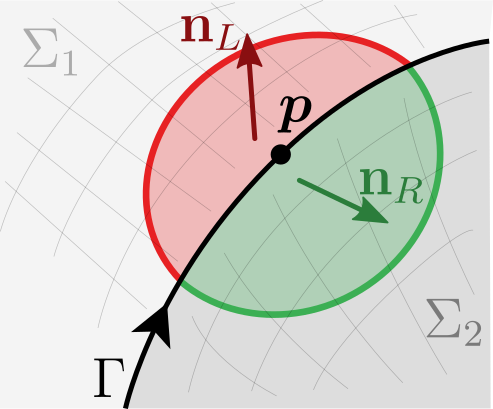
\includegraphics[width=5cm]{voisinage_courbe_singuliere.png}
%    \caption{Voisinage d'un point sur une courbe singulière.}
%\end{figure}



\section{Observations}%/Motivations}
[Objectif : justifier en quoi la construction intermédiaire d'une \guillemets{EdS partielle} (sous-ensemble de l'EdS qui contient l'EdB) permet de simplifier la construction d'un modèle \brep\ de l'EdB en évitant de construire des éléments de l'EdS qui sont trivialement exclues de l'EdB]
\par
définitions : 
\begin{itemize}
	\item \textit{zone d'influence}\footnote{\label{note_vocabulaire_notation}vocabulaire et notation à préciser \ldots} de $H \subseteq \Sigma$ sur l'EdB  (lieu des points de tangence entre $\EdB{\Sigma}{\rho}$ et $\sphere[H][\rho]$)
	\[ \influEdB{H}{\rho} := \EdB{\Sigma}{\rho} \cap \sphere[H][\rho] \]
	\item \textit{EdS propre}\footref{note_vocabulaire_notation} de $H \subseteq \Sigma$ 
	\[ \EdSpropre{H}{\rho} := \closure{ {\EdS{H}{\rho} \setminus \EdS{\boundary{H}}{\rho}} } \]
\end{itemize}
arguments :
\begin{enumerate}
	\item on sait décrire l'EdB simplement de manière \textit{implicite} (\cf \autoref{section:principe_huygens}) mais on cherche à en construire une représentation \textit{explicite}
	\item en revanche, on peut décrire explicitement l'EdS de chaque carreau ($\to$ introduire système définissant l'EdS à 2 paramètres)
	\item il est plus commode de voir l'EdS d'un carreau comme (un sous-ensemble de) la réunion de 10 nouveaux carreaux (intérieur $\to 2$ , bords $\to 4$ et ``coins'' $\to 4$)
	\item si on procède ainsi pour chaque carreau qui décrit l'interface, on construit beaucoup de nouveaux carreaux qui sont redondants, voire même trivialement exclus de l'EdB
%	\item la zone d'influence sur l'EdB d'une courbe singulière concave est vide (preuve?) (\ie cette courbe ne contribue pas à l'EdB et peut donc être ignorée)
%	\item la zone d'influence sur l'EdB d'une courbe singulière convexe $\Gamma$ est incluse dans la portion de son EdS qui est tangente aux EdS des deux nappes adhérentes à $\Gamma$ (preuve?), on appelle cette portion \textit{pseudo-EdS}\footref{note_vocabulaire_notation} de $\Gamma$ et on la note $\pseudoEdS{\Gamma}{\rho}$
	\item La zone d'influence sur l'EdB d'une courbe $\Gamma \subset \Sigma$ adhérentes aux nappes régulières $\Sigma_L$ et $\Sigma_R$ est incluse dans le lieu des points de tangence entre $\EdS{\Gamma}{\rho}$, $\EdS{\Sigma_L}{\rho}$ et $\EdS{\Sigma_R}{\rho}$ (on appelle ce lieu \textit{pseudo-EdS}\footref{note_vocabulaire_notation} de $\Gamma$ et on le note $\pseudoEdS{\Gamma}{\rho}$).
	\begin{proof}
		En posant\footnote{introduire ces notations dans la \autoref{section:principe_huygens}.}
		\[
			\implicitsphere(\bx, \p) := \normtwo{\bx - \p}^2 - \rho(\p)^2,
		\]
		et, pour $H \subseteq \Sigma$, 
		\[
			\implicitEdB{H}(\bx) := \min_{\p \in H} \implicitsphere(\bx, \p),
		\]
		on veut démontrer que 
		\[
			\influEdB{\Gamma}{\rho} \subseteq 
			\left\{
				\bx \in \complement{\Omega} \mid \implicitEdB{\Gamma}(\bx) = \implicitEdB{\Sigma_L}(\bx) = \implicitEdB{\Sigma_R}(\bx) = 0
			\right\}
			\subseteq \pseudoEdS{\Gamma}{\rho}.
		\]
		\par
		Puisque $\Gamma \subseteq \left( \closure{\Sigma_L} \cap \closure{\Sigma_R} \right)$, on a $\implicitEdB{\Gamma} \geq \implicitEdB{\Sigma_L}$ et $\implicitEdB{\Gamma} \geq \implicitEdB{\Sigma_R}$.\par
		Or, si $\bx \in \influEdB{\Gamma}{\rho}$ alors\footnote{car $\forall \bx \in \EdB{\Sigma}{\rho}, \implicitEdB{\Gamma}(\bx) \geq 0$ et $\forall \bx \in \sphere[\Gamma][\rho], \implicitEdB{\Gamma}(\bx) \leq 0$.} $\implicitEdB{\Gamma}(\bx) = 0$ et donc $\implicitEdB{\Sigma_L}(\bx) \leq 0$ et $\implicitEdB{\Sigma_R}(\bx) \leq 0$.\par
		Mais si $\implicitEdB{\Sigma_L} < 0$ ou $\implicitEdB{\Sigma_R} < 0$ alors\footnote{car $\forall H \subseteq \Sigma, \forall \bx \in \EdB{\Sigma}{\rho}, \implicitEdB{H}(\bx) \geq 0$.} $\bx \notin \EdB{\Sigma}{\rho}$ et donc $\bx \notin \influEdB{\Gamma}{\rho}$.\par
		Donc si $\bx \in \influEdB{\Gamma}{\rho}$ alors $\implicitEdB{\Sigma_L}(\bx) = 0$ et $\implicitEdB{\Sigma_R}(\bx) = 0$.
	\end{proof}
	
	\item Si $\Gamma$ est une courbe singulière concave de $\Sigma$ alors sa zone d'influence sur l'EdB est vide (\ie $\Gamma$ ne contribue pas à l'EdB et peut donc être ignorée).
	\begin{proof}
		On veut montrer que $\influEdB{\Gamma}{\rho} = \varnothing$ (piste : montrer que, pour $\bx \in \complement{\Omega}$, $\implicitEdB{\Gamma}(\bx) = 0 \Rightarrow \implicitEdB{\Sigma_L}(\bx) < 0$ ou $\implicitEdB{\Sigma_R}(\bx) < 0$)
	\end{proof}
	
	\item si toutes les courbes singulières adhérentes à un point singulier sont concaves alors la zone d'influence sur l'EdB de ce point est vide (preuve?) (\ie ce point ne contribue pas à l'EdB et peut donc être ignoré)
	\item si toutes les courbes singulières adhérentes à un point singulier $\p$ \textit{ne sont pas} concaves (ou bien que $\p$ n'est adhérent à aucune courbe singulière, \eg le sommet d'un cône) on dit que $\p$ est convexe et sa zone d'influence sur l'EdB est la portion de $\sphere[\p][\rho(\p)]$ qui est tangente aux EdS de toutes les courbes singulières adhérentes à $\p$ (preuve?), on appelle cette portion \textit{pseudo-EdS}\footref{note_vocabulaire_notation} de $\p$ et on la note $\pseudoEdS{\p}{\rho}$
	\item l'EdB est incluse dans la réunion
	\begin{itemize}
		\item des EdS propres des nappes régulières, qui sont elles-mêmes contenues dans la réunion des EdS propres des faces \brep
		\item des pseudo-EdS des courbes singulières convexes, qui sont elles-mêmes contenues dans la réunion des pseudo-EdS des arêtes \brep\ convexes
		\item des pseudo-EdS des points singuliers convexes, qui sont elles-mêmes contenues dans la réunion des pseudo-EdS des sommets \brep\ convexes
	\end{itemize}
	\item[$\Rightarrow$] on construit d'abord une telle réunion (que l'on appelle \textit{EdS partielle}\footref{note_vocabulaire_notation}) puis on en élimine les régions qui sont exclues de l'EdB (au passage on constitue les relations topologiques qui assurent la validité du modèle \brep)
\end{enumerate}



\setlength{\imagewidth}{50mm}%
\setlength{\imageheight}{\imagewidth}%
\begin{figure}
	\centering
%	\definecolor{colorContourEdSnappe0}{rgb}{1,0,0}
%	\definecolor{colorContourEdSnappe1}{rgb}{0,1,0}
%	\definecolor{colorContourEdSarete}{rgb}{0,0,1}
	\colorlet{colorContourEdSnappe0}{mycolor_2}
	\colorlet{colorContourEdSnappe1}{mycolor_3}
	\colorlet{colorContourEdSarete}{mycolor_1}
	\colorlet{colorInterieurEdSnappe0}{colorContourEdSnappe0}%!50!white}
	\colorlet{colorInterieurEdSnappe1}{colorContourEdSnappe1}%!50!white}
	\colorlet{colorInterieurarete}{colorContourEdSarete!30!white}
	\colorlet{colorPseudoEdSarete}{mycolor_4}%colorContourEdSarete!70!black}
	\begin{tikzpicture}[
		x = \imagewidth,
		y = \imageheight,
		styleEdS/.style = {
			thick, fill opacity=0.2
		},
		stylePseudoEdS/.style = {
			line width=1.1pt, colorPseudoEdSarete, line cap=round%, dash pattern=on 4pt off 3pt
		},
		styleNappe/.style = {
			draw=black, thick, line cap=round
		}
	]
		\begin{scope}
			%\clip (-1,-0.55) rectangle (1,0.8);
			\begin{scope}[blend group = overlay]
\draw[styleEdS, draw=colorContourEdSnappe0, fill=colorInterieurEdSnappe0] 
(1.0398871880695557, -0.05029176412270403) -- 
(1.0183167534800655, -0.0449025730216131) -- 
(0.9970249326809821, -0.03889063165462239) -- 
(0.9760087070839042, -0.03227375493086215) -- 
(0.9552635663797575, -0.025069985986572035) -- 
(0.9347833891410695, -0.017297348539330626) -- 
(0.9145603833626653, -0.008973612328943836) -- 
(0.8945850834066453, -0.00011607984793962633) -- 
(0.8748463978997224, 0.009258598781243438) -- 
(0.8553317017006214, 0.019134577567845562) -- 
(0.83602696412914, 0.029496929643137104) -- 
(0.816916905210558, 0.04033172390652845) -- 
(0.7979851716958212, 0.05162606350851576) -- 
(0.7792145250047978, 0.06336808792773979) -- 
(0.7605870339290941, 0.07554694172716503) -- 
(0.742084265838364, 0.08815271410883804) -- 
(0.7236874711762205, 0.10117635410812229) -- 
(0.7053777571313378, 0.11460956667949797) -- 
(0.68713624745879, 0.12844469504848804) -- 
(0.6689442264517612, 0.1426745945736954) -- 
(0.650783265984124, 0.1572925030243364) -- 
(0.6326353353336946, 0.1722919116818077) -- 
(0.6144828941409042, 0.18766644106904284) -- 
(0.5963089693558062, 0.20340972444626615) -- 
(0.5780972173844605, 0.21951530152848314) -- 
(0.5598319728767698, 0.2359765242139565) -- 
(0.5414982857190578, 0.2527864754915883) -- 
(0.5230819478253321, 0.26993790213828667) -- 
(0.5045695112809123, 0.28742316133741974) -- 
(0.4859482992996188, 0.3052341809521778) -- 
(0.4672064113277807, 0.3233624328735336) -- 
(0.4483327234793507, 0.34179891862769246) -- 
(0.4293168853280881, 0.36053416626560775) -- 
(0.4101493139242216, 0.37955823745850226) -- 
(0.3908211857508439, 0.3988607436785092) -- 
(0.3713244271940277, 0.4184308703424265) -- 
(0.35165170397301176, 0.4382574078293584) -- 
(0.33179640986407155, 0.4583287883406225) -- 
(0.3117526549541225, 0.4786331276446601) -- 
(0.291515253577205, 0.4991582708338544) -- 
(0.28440988145616547, 0.5063087863339162) -- 
(0.27710254029824977, 0.5132527729480235) -- 
(0.2695992307813853, 0.5199845283794992) -- 
(0.26190611450974904, 0.5264985246127) -- 
(0.25402950895395104, 0.5327894124525396) -- 
(0.24597588226322395, 0.5388520259171669) -- 
(0.23775184795387602, 0.5446813864801907) -- 
(0.2293641594783722, 0.5502727071589723) -- 
(0.22081970467950082, 0.5556213964456214) -- 
(0.2121255001341817, 0.5607230620774737) -- 
(0.20328868539155925, 0.5655735146439503) -- 
(0.19431651711011275, 0.5701687710268386) -- 
(0.18521636309859835, 0.5745050576711679) -- 
(0.17599569626571607, 0.5785788136839961) -- 
(0.1666620884834703, 0.5823866937585616) -- 
(0.1572232043692633, 0.5859255709213973) -- 
(0.147686794991827, 0.5891925391001548) -- 
(0.13806069150616307, 0.592184915510027) -- 
(0.1283527987227171, 0.59490024285681) -- 
(0.1185710886160675, 0.597336291354796) -- 
(0.10872359377846114, 0.5994910605578396) -- 
(0.09881840082356977, 0.6013627810020942) -- 
(0.0888636437458856, 0.6029499156590681) -- 
(0.07886749724120823, 0.6042511611978101) -- 
(0.06883816999370787, 0.6052654490551841) -- 
(0.058783897935078405, 0.6059919463133578) -- 
(0.048712937481315166, 0.606430056383782) -- 
(0.038633558752670744, 0.6065794194970995) -- 
(0.028554038782357544, 0.6064399129985829) -- 
(0.018482654719573693, 0.6060116514488569) -- 
(0.008427677032433106, 0.6052949865298223) -- 
(-0.0016026372836175917, 0.6042905067558604) -- 
(-0.011600051486318735, 0.602999036990554) -- 
(-0.02155635585048546, 0.601421637769322) -- 
(-0.031463374409710254, 0.5995596044285232) -- 
(-0.04131297167034209, 0.5974144660417463) -- 
(-0.051097059292231184, 0.5949879841641577) -- 
(-0.06080760273075139, 0.592282151385939) -- 
(-0.07043662783464624, 0.5892991896960018) -- 
(-0.07997622739428173, 0.5860415486573246) -- 
(-0.08941856763492664, 0.5825119033954085) -- 
(-0.09875589464973036, 0.5787131524015046) -- 
(-0.10798054076711328, 0.5746484151524166) -- 
(-0.11708493084734278, 0.5703210295488347) -- 
(-0.12606158850312335, 0.5657345491743005) -- 
(-0.1349031422390926, 0.5608927403770597) -- 
(-0.14360233150518156, 0.5557995791771925) -- 
(-0.15215201265886868, 0.550459248001567) -- 
(-0.16054516483143072, 0.5448761322492933) -- 
(-0.16877489569337395, 0.5390548166905) -- 
(-0.17683444711431084, 0.5330000817013907) -- 
(-0.18471720071263423, 0.526716899338671) -- 
(-0.19241668329043216, 0.5202104292565717) -- 
(-0.19992657214918022, 0.5134860144698171) -- 
(-0.2072407002818455, 0.5065491769660245) -- 
(-0.2143530614371397, 0.49940561317112975) -- 
(-0.22125781505176162, 0.4920611892715692) -- 
(-0.22794929104657935, 0.48452193639705643) -- 
(-0.23442199448281317, 0.4767940456679094) -- 
(-0.24067061007439672, 0.4688838631109964) -- 
(-0.24669000655280857, 0.4607978844484749) -- 
(-0.252475240880793, 0.45254274976360276) -- 
(-0.25802156231150697, 0.44412523804800214) -- 
(-0.2633244162897616, 0.43555226163485494) -- 
(-0.2683794481921539, 0.42683086052259867) -- 
(-0.2731825069030178, 0.4179681965937866) -- 
(-0.2777296482232569, 0.4089715477338585) -- 
(-0.2820171381092618, 0.39984830185465114) -- 
(-0.2860414557392498, 0.39060595082755645) -- 
(-0.28979929640451024, 0.38125208433131086) -- 
(-0.2932875742231817, 0.3717943836194658) -- 
(-0.2965034246743312, 0.3622406152126584) -- 
(-0.29944420695025553, 0.35259862452086255) -- 
(-0.3021075061250724, 0.3428763294008567) -- 
(-0.30449113513782133, 0.3330817136542001) -- 
(-0.30659313658844445, 0.3232228204710559) -- 
(-0.3084117843451744, 0.31330774582524457) -- 
(-0.30994558496200736, 0.30334463182595317) -- 
(-0.31119327890509796, 0.29334166003155904) -- 
(-0.31215384158707016, 0.2833070447310568) -- 
(-0.312826484208392, 0.2732490261986096) -- 
(-0.3132106544051267, 0.2631758639267602) -- 
(-0.3133060367025248, 0.2530958298438609) -- 
(-0.31311255277408784, 0.24301720152129108) -- 
(-0.3126303615058885, 0.23294825537604125) -- 
(-0.311859858866096, 0.22289725987424416) -- 
(-0.31080167757981286, 0.21287246874123647) -- 
(-0.3094566866094909, 0.20288211418372343) -- 
(-0.30782599044135184, 0.19293440012961588) -- 
(-0.3059109281784007, 0.18303749549108922) -- 
(-0.30371307244077433, 0.1731995274563957) -- 
(-0.3012342280743293, 0.16342857481594059) -- 
(-0.29847643066853036, 0.15373266132810265) -- 
(-0.2954419448848546, 0.14411974913024406) -- 
(-0.29213326259708616, 0.13459773220032423) -- 
(-0.28855310084502717, 0.12517442987448518) -- 
(-0.2847043996033055, 0.11585758042593017) -- 
(-0.2805903193671125, 0.10665483471037143) -- 
(-0.27621423855685184, 0.09757374988326305) -- 
(-0.2715797507438321, 0.08862178319397956) -- 
(-0.26669066169928013, 0.07980628586203543) -- 
(-0.26155098626909984, 0.07113449704037526) -- 
(-0.25616494507694093, 0.0626135378706904) -- 
(-0.2505369610582869, 0.0542504056356455) -- 
(-0.2446716558284075, 0.0460519680128164) -- 
(-0.23857384588715833, 0.03802495743505638) -- 
(-0.23224853866374337, 0.030175965561924676) -- 
(-0.2257009284046912, 0.022511437866715802) -- 
(-0.218936391908417, 0.015037668343533813) -- 
(-0.2119604841098781, 0.0077607943387599816) -- 
(-0.20477893351894494, 0.0006867915111568382) -- 
(-0.19739763751623587, -0.006178531075252337) -- 
(-0.18982265751027697, -0.0128295357214991) -- 
(-0.18206021395996608, -0.019260760723262417) -- 
(-0.17411668126642477, -0.025466924855938287) -- 
(-0.1659985825384379, -0.0314429317115007) -- 
(-0.13814675776047186, -0.051389728187050454) -- 
(-0.11010149732607256, -0.07084782564879044) -- 
(-0.08187628874232598, -0.08980691529833429) -- 
(-0.05348514223118164, -0.10825785303989452) -- 
(-0.024942488161001697, -0.1261927311153278) -- 
(0.0037369331581589837, -0.14360494415097552) -- 
(0.032538188799990014, -0.16048924853161478) -- 
(0.0614462769517472, -0.17684181400939064) -- 
(0.09044625611895998, -0.19266026647310083) -- 
(0.11952337865593937, -0.20794372084870297) -- 
(0.14866322725437772, -0.22269280317764836) -- 
(0.17785185281340019, -0.23690966102675073) -- 
(0.2070759119251168, -0.25059796152153513) -- 
(0.2363228020507566, -0.26376287646259583) -- 
(0.265580792345058, -0.2764110541778851) -- 
(0.29483914802179645, -0.2885505779777789) -- 
(0.32408824615147613, -0.30019091130722525) -- 
(0.35331968085209736, -0.3113428299218043) -- 
(0.38252635598214596, -0.32201834164250964) -- 
(0.4117025636751192, -0.33223059445727054) -- 
(0.4408440473670057, -0.3419937739254134) -- 
(0.46994804835801024, -0.3513229909948436) -- 
(0.49901333540890813, -0.3602341614525258) -- 
(0.5280402173876334, -0.36874387829068567) -- 
(0.5570305395358062, -0.37686927828051764) -- 
(0.58598766449683, -0.38462790400140734) -- 
(0.6149164398129897, -0.39203756247917254) -- 
(0.6438231541327407, -0.39911618144689354) -- 
(0.6727154848442609, -0.40588166406421605) -- 
(0.7016024402409139, -0.41235174272506525) -- 
(0.7304942996033684, -0.4185438323598505) -- 
(0.7594025547290846, -0.4244748834068749) -- 
(0.788339856433129, -0.4301612343982981) -- 
(0.8173199693690699, -0.43561846388665537) -- 
(0.8463577381635287, -0.44086124123470705) -- 
(0.8754690673157085, -0.44590317560849646) -- 
(0.9046709165817106, -0.4507566623537582) -- 
(0.9339813126454302, -0.4554327258016044) -- 
(0.9634193767817649, -0.4599408574440896) -- 
(0.9693155652265435, -0.4609052976013954) -- 
(0.9752369803674806, -0.4617002980555111) -- 
(0.9811787540119019, -0.4623252052100757) -- 
(0.9871360012297284, -0.462779505308097) -- 
(0.9931038243695415, -0.46306282485432837) -- 
(0.9990773170851042, -0.4631749309223312) -- 
(1.0050515683690329, -0.463115731345972) -- 
(1.0110216665902994, -0.4628852747951948) -- 
(1.0169827035322463, -0.46248375073600834) -- 
(1.022929778427797, -0.46191148927471937) -- 
(1.0288580019885372, -0.46116896088654163) -- 
(1.0347625004243635, -0.4602567760288024) -- 
(1.0406384194503882, -0.45917568463906483) -- 
(1.0464809282778087, -0.45792657551857996) -- 
(1.0522852235854594, -0.45651047560157293) -- 
(1.0580465334687832, -0.45492854911096664) -- 
(1.0637601213629715, -0.453182096601235) -- 
(1.0694212899370539, -0.4512725538891737) -- 
(1.0750253849557292, -0.4492014908734677) -- 
(1.0805677991057672, -0.4469706102440253) -- 
(1.0860439757838356, -0.4445817460821393) -- 
(1.0914494128426344, -0.4420368623526284) -- 
(1.0967796662922613, -0.439338051289196) -- 
(1.1020303539537641, -0.4364875316743353) -- 
(1.1071971590618763, -0.43348764701519416) -- 
(1.1122758338139729, -0.4303408636168996) -- 
(1.1172622028623307, -0.42704976855492677) -- 
(1.1221521667468217, -0.42361706754817735) -- 
(1.1269417052652146, -0.4200455827345184) -- 
(1.1316268807783172, -0.41633825035060845) -- 
(1.1362038414472417, -0.41249811831791966) -- 
(1.1406688244001288, -0.4085283437369402) -- 
(1.1450181588257307, -0.40443219029161614) -- 
(1.1492482689913066, -0.40021302556616906) -- 
(1.153355677182352, -0.3958743182764921) -- 
(1.1573370065617445, -0.3914196354184033) -- 
(1.161188983945953, -0.3868526393350996) -- 
(1.1649084424960312, -0.3821770847062224) -- 
(1.1684923243211818, -0.37739681546101034) -- 
(1.1719376829927497, -0.372515761618077) -- 
(1.1752416859665806, -0.36753793605441143) -- 
(1.1784016169117477, -0.3624674312062588) -- 
(1.18141487794374, -0.35730841570459176) -- 
(1.1842789917602683, -0.3520651309479401) -- 
(1.186991603677939, -0.346741887615396) -- 
(1.1895504835681168, -0.3413430621226607) -- 
(1.1919535276903879, -0.33587309302404755) -- 
(1.1941987604221163, -0.33033647736339883) -- 
(1.196284335882667, -0.32473776697691586) -- 
(1.1982085394509678, -0.31908156475094274) -- 
(1.1999697891751553, -0.3133725208377806) -- 
(1.2015666370731508, -0.30761532883264203) -- 
(1.202997770323094, -0.30181472191489017) -- 
(1.2042620123426586, -0.2959754689567343) -- 
(1.2053583237563583, -0.2901023706025812) -- 
(1.206285803250054, -0.2842002553222653) -- 
(1.207043688311952, -0.27827397544140275) -- 
(1.2076313558594922, -0.272328403152133) -- 
(1.2080483227516046, -0.2663684265075271) -- 
(1.2082942461859139, -0.2603989454029569) -- 
(1.2083689239805722, -0.25442486754772686) -- 
(1.2082722947404756, -0.24845110443028384) -- 
(1.2080044379077421, -0.24248256728031795) -- 
(1.2075655736963986, -0.2365241630310776) -- 
(1.206956062911335, -0.2305807902852156) -- 
(1.2061764066516745, -0.22465733528748522) -- 
(1.2052272458988051, -0.2187586679075953) -- 
(1.2041093609894056, -0.21288963763652835) -- 
(1.2028236709739044, -0.20705506959961203) -- 
(1.2013712328609003, -0.20125976058962325) -- 
(1.1997532407481573, -0.19550847512318478) -- 
(1.1979710248408986, -0.18980594152369779) -- 
(1.1960260503582012, -0.18415684803402882) -- 
(1.1939199163283891, -0.17856583896215006) -- 
(1.1916543542744191, -0.1730375108628982) -- 
(1.1892312267903393, -0.16757640875899452) -- 
(1.186652526009987, -0.1621870224044293) -- 
(1.1839203719691895, -0.15687378259328583) -- 
(1.1810370108628132, -0.15164105751703733) -- 
(1.1780048131980896, -0.14649314917331077) -- 
(1.1748262718457447, -0.14143428982907139) -- 
(1.1715039999905257, -0.13646863854113506) -- 
(1.1680407289828147, -0.13160027773686905) -- 
(1.164439306093095, -0.12683320985789287) -- 
(1.1607026921711152, -0.12217135406953673) -- 
(1.156833959211675, -0.11761854303876616) -- 
(1.1528362878290375, -0.11317851978321818) -- 
(1.1487129646420393, -0.10885493459394213) -- 
(1.1444673795720515, -0.10465134203437362) -- 
(1.1401030230560127, -0.1005711980180092) -- 
(1.1356234831768246, -0.09661785696718544) -- 
(1.1310324427134695, -0.09279456905529601) -- 
(1.1263336761132745, -0.08910447753471601) -- 
(1.1215310463888133, -0.08555061615262943) -- 
(1.1166285019419941, -0.0821359066568845) -- 
(1.1116300733179485, -0.07886315639392778) -- 
(1.1065398698913833, -0.0757350560007904) -- 
(1.1013620764881287, -0.07275417719302638) -- 
(1.0961009499446528, -0.06992297065041925) -- 
(1.090760815608376, -0.06724376400219671) -- 
(1.0853460637816557, -0.06471875991340899) -- 
(1.0798611461123757, -0.06235003427404442) -- 
(1.0743105719340957, -0.060139534492371444) -- 
(1.0686989045587796, -0.058089077893909054) -- 
(1.0630307575251439, -0.05620035022734317) -- 
(1.057310790805714, -0.05447490427861628) -- 
(1.0515437069757052, -0.052914158594330525) -- 
(1.0457342473468798, -0.05151939631551329) -- 
cycle; 
\coordinate (EdS0) at (0.5780972173844605, 0.21951530152848314);
\draw[styleEdS, draw=colorContourEdSnappe1, fill=colorInterieurEdSnappe1] 
(-0.15169069257764084, 0.5507561630088252) -- 
(-0.17504146443852367, 0.5360596714869722) -- 
(-0.1980509650850808, 0.521674771969309) -- 
(-0.22073415534445154, 0.5076006935349764) -- 
(-0.24310719678293558, 0.49383615486428445) -- 
(-0.2651874165214464, 0.48037937081071636) -- 
(-0.2869932690927314, 0.46722807665123334) -- 
(-0.3085442956789244, 0.4543795691229797) -- 
(-0.32986108091481187, 0.44183076319743253) -- 
(-0.35096520730549785, 0.42957826339985106) -- 
(-0.37187920718936585, 0.41761844835234146) -- 
(-0.3926265120789917, 0.40594756710319946) -- 
(-0.4132313991330905, 0.39456184570400504) -- 
(-0.4337189344495226, 0.3834576024096734) -- 
(-0.45411491281992367, 0.3726313698053583) -- 
(-0.47444579354746064, 0.3620800221069333) -- 
(-0.49473863189786793, 0.35180090583672363) -- 
(-0.5150210057287882, 0.34179197203978184) -- 
(-0.5353209368240557, 0.33205190817334773) -- 
(-0.5556668064512493, 0.3225802677669589) -- 
(-0.5760872646692548, 0.313377595905848) -- 
(-0.5966111329481912, 0.3044455485284712) -- 
(-0.6172672997411849, 0.29578700344381215) -- 
(-0.6380846087839275, 0.2874061608610278) -- 
(-0.6590917401143961, 0.27930863108194903) -- 
(-0.6803170841236117, 0.2715015068394799) -- 
(-0.7017886093907949, 0.2639934175814647) -- 
(-0.7235337256421194, 0.25679456281626867) -- 
(-0.7455791439158018, 0.24991672147641975) -- 
(-0.7679507369237274, 0.2433732341503716) -- 
(-0.790673403666179, 0.23717895501566963) -- 
(-0.8137709435620123, 0.23135017041918954) -- 
(-0.837265946664578, 0.22590448133181817) -- 
(-0.8611797078861451, 0.22086064739230282) -- 
(-0.8855321744698602, 0.21623839097508424) -- 
(-0.9103419371234759, 0.21205816068103941) -- 
(-0.9356262761334505, 0.20834085484647802) -- 
(-0.961401274258467, 0.20510750705228062) -- 
(-0.9876820080846747, 0.20237893711210087) -- 
(-1.0144828286234011, 0.20017537250377648) -- 
(-1.0212111055321056, 0.19966127297052094) -- 
(-1.0279217854342695, 0.19895361221776484) -- 
(-1.034609301063352, 0.19805297732998992) -- 
(-1.041268104370191, 0.1969601154855073) -- 
(-1.0478926711257381, 0.19567593333658903) -- 
(-1.0544775055040283, 0.194201496257298) -- 
(-1.0610171446415886, 0.19253802745963902) -- 
(-1.0675061631695015, 0.19068690697876728) -- 
(-1.0739391777143585, 0.18864967052809295) -- 
(-1.080310851364378, 0.18642800822523345) -- 
(-1.086615898096975, 0.18402376318987038) -- 
(-1.092849087164114, 0.18143893001467354) -- 
(-1.0990052474318048, 0.1786756531105611) -- 
(-1.105079271670143, 0.17573622492766872) -- 
(-1.1110661207903312, 0.17262308405350335) -- 
(-1.116960828025175, 0.1693388131898597) -- 
(-1.122758503049575, 0.16588613701017735) -- 
(-1.1284543360376047, 0.1622679198991166) -- 
(-1.134043601652803, 0.15848716357622827) -- 
(-1.1395216629683755, 0.15454700460568818) -- 
(-1.1448839753140478, 0.1504507117941632) -- 
(-1.1501260900463823, 0.146201683478967) -- 
(-1.1552436582394316, 0.14180344470875594) -- 
(-1.1602324342926624, 0.13725964431910287) -- 
(-1.1650882794531596, 0.13257405190537624) -- 
(-1.1698071652491915, 0.12775055469543542) -- 
(-1.1743851768322795, 0.12279315432473595) -- 
(-1.1788185162250082, 0.11770596351652171) -- 
(-1.1831035054718757, 0.11249320266985613) -- 
(-1.1872365896905732, 0.10715919635832517) -- 
(-1.1912143400211617, 0.1017083697423152) -- 
(-1.195033456470697, 0.09614524489784283) -- 
(-1.1986907706509484, 0.09047443706498239) -- 
(-1.2021832484069326, 0.08470065081900341) -- 
(-1.2055079923340877, 0.07882867616739407) -- 
(-1.2086622441819999, 0.07286338457600965) -- 
(-1.2116433871426804, 0.06680972492764123) -- 
(-1.2144489480215048, 0.06067271941635902) -- 
(-1.2170765992890076, 0.054457459381035425) -- 
(-1.2195241610118286, 0.048169101081504476) -- 
(-1.2217896026612163, 0.04181286142086249) -- 
(-1.223871044797579, 0.03539401361745781) -- 
(-1.225766760629692, 0.028917882830160894) -- 
(-1.2274751774472679, 0.022389841740544255) -- 
(-1.228994877925694, 0.01581530609563598) -- 
(-1.2303246013018665, 0.00919973021494658) -- 
(-1.2314632444201337, 0.002548602465495202) -- 
(-1.2324098626474882, -0.004132559291410428) -- 
(-1.2331636706572482, -0.010838212277863062) -- 
(-1.2337240430805723, -0.017562793397715527) -- 
(-1.2340905150252757, -0.024300723851797427) -- 
(-1.2342627824615098, -0.03104641376615843) -- 
(-1.2342407024739888, -0.03779426682950015) -- 
(-1.2340242933805552, -0.04453868493594776) -- 
(-1.2336137347169822, -0.05127407282931096) -- 
(-1.2330093670880287, -0.05799484274498075) -- 
(-1.2322116918848693, -0.06469541904561071) -- 
(-1.2312213708691342, -0.07137024284673765) -- 
(-1.2300392256239019, -0.0780137766285043) -- 
(-1.2286662368721049, -0.08462050882965623) -- 
(-1.2271035436629079, -0.09118495842000482) -- 
(-1.2253524424267392, -0.09770167944756064) -- 
(-1.2234143858997542, -0.10416526555656458) -- 
(-1.2212909819186275, -0.11057035447267138) -- 
(-1.2189839920866703, -0.11691163245156061) -- 
(-1.2164953303123824, -0.1231838386872879) -- 
(-1.213827061221648, -0.12938176967671738) -- 
(-1.2109813984448963, -0.13550028353641472) -- 
(-1.2079607027806447, -0.14153430426842012) -- 
(-1.2047674802369503, -0.14747882597136147) -- 
(-1.201404379952393, -0.15332891699341478) -- 
(-1.1978741919983158, -0.15907972402366605) -- 
(-1.1941798450641463, -0.1647264761184806) -- 
(-1.1903244040277179, -0.17026448865953914) -- 
(-1.1863110674126072, -0.17568916724025793) -- 
(-1.182143164734598, -0.18099601147736766) -- 
(-1.1778241537394727, -0.1861806187444887) -- 
(-1.1733576175344205, -0.1912386878246079) -- 
(-1.1687472616154468, -0.19616602247842244) -- 
(-1.1639969107932449, -0.20095853492559496) -- 
(-1.1591105060200841, -0.2056122492360284) -- 
(-1.154092101120346, -0.2101233046283487) -- 
(-1.1489458594274173, -0.21448795867285936) -- 
(-1.1436760503297374, -0.21870259039630863) -- 
(-1.1382870457288554, -0.22276370328589631) -- 
(-1.1327833164124483, -0.22666792819002524) -- 
(-1.1271694283452947, -0.23041202611339306) -- 
(-1.1214500388812925, -0.23399289090410488) -- 
(-1.1156298928996586, -0.23740755183057632) -- 
(-1.1097138188685158, -0.2406531760460909) -- 
(-1.1037067248391326, -0.2437270709389667) -- 
(-1.0976135943741416, -0.24662668636638074) -- 
(-1.0914394824131113, -0.24934961677000123) -- 
(-1.085189511078903, -0.2518936031716694) -- 
(-1.0788688654282916, -0.2542565350474768) -- 
(-1.072482789150376, -0.2564364520786833) -- 
(-1.0660365802163472, -0.25843154577802285) -- 
(-1.059535586484222, -0.26024016099004743) -- 
(-1.052985201262192, -0.261860797264266) -- 
(-1.0463908588342665, -0.26329211009993686) -- 
(-1.0397580299519174, -0.2645329120614833) -- 
(-1.0330922172954773, -0.26558217376360543) -- 
(-1.0263989509090414, -0.2664390247252709) -- 
(-1.0196837836126742, -0.26710275409187817) -- 
(-1.0129522863957163, -0.2675728112249897) -- 
(-1.0062100437950219, -0.2678488061591494) -- 
(-0.9994626492619538, -0.2679305099254024) -- 
(-0.9927157005219838, -0.2678178547412513) -- 
(-0.9618600215907757, -0.26718218439906705) -- 
(-0.9312831146272719, -0.2666713947766457) -- 
(-0.9009530059793759, -0.26625843546062694) -- 
(-0.8708379447198517, -0.2659148207309584) -- 
(-0.8409063796084735, -0.26561086314225923) -- 
(-0.8111270158339738, -0.2653158722753026) -- 
(-0.781468939498758, -0.2649983223125783) -- 
(-0.7519017969860202, -0.26462599327495656) -- 
(-0.7223960161469252, -0.26416609165852906) -- 
(-0.6929230564929207, -0.2635853567615401) -- 
(-0.6634556761362759, -0.26285015915721244) -- 
(-0.6339682039861398, -0.26192659754746617) -- 
(-0.6044368066058047, -0.2607805996498903) -- 
(-0.5748397401256944, -0.2593780318721067) -- 
(-0.5451575786645209, -0.25768482137646576) -- 
(-0.5153734118323504, -0.2556670928082199) -- 
(-0.48547300507696894, -0.25329132053369574) -- 
(-0.4554449178937359, -0.25052449579649216) -- 
(-0.4252805762499636, -0.24733430683318938) -- 
(-0.3949742969699929, -0.24368932877385877) -- 
(-0.36452326326741585, -0.23955921915536818) -- 
(-0.33392745206468954, -0.23491491415179303) -- 
(-0.30318951516469345, -0.2297288202133098) -- 
(-0.2723146176820055, -0.2239749957199047) -- 
(-0.241310238347933, -0.21762931749468523) -- 
(-0.21018593731769367, -0.2106696275580442) -- 
(-0.17895309788205088, -0.203075856293629) -- 
(-0.14762464898207767, -0.1948301191796247) -- 
(-0.1162147756228702, -0.18591678534310513) -- 
(-0.0847386241761405, -0.17632251734497642) -- 
(-0.05321200916732435, -0.16603628272319448) -- 
(-0.02165112749206638, -0.1550493388439899) -- 
(0.009927714853966221, -0.14335519347778738) -- 
(0.041508359462259836, -0.130949544186216) -- 
(0.07307503265108445, -0.11783020005372988) -- 
(0.1046125612256801, -0.1039969895135833) -- 
(0.13610656612738772, -0.08945165801084692) -- 
(0.16754363425536342, -0.07419775903601292) -- 
(0.19891146963183234, -0.058240541683307556) -- 
(0.2078176233741046, -0.053513397115755326) -- 
(0.21658463702996975, -0.04853294113247408) -- 
(0.22520530776875866, -0.04330326559216415) -- 
(0.23367255299267653, -0.03782866710811363) -- 
(0.2419794161557458, -0.032113643518173626) -- 
(0.25011907247918735, -0.026162890189410426) -- 
(0.25808483455854336, -0.01998129616047086) -- 
(0.2658701578579365, -0.013573940124830638) -- 
(0.27346864608695, -0.006946086258225556) -- 
(0.2808740564557121, -0.00010317989369318381) -- 
(0.28808030480386737, 0.006949156952220904) -- 
(0.29508147059921985, 0.014205130198417112) -- 
(0.3018718018019427, 0.021658778459561226) -- 
(0.3084457195903571, 0.029303977943858264) -- 
(0.3147978229443984, 0.03713444748425651) -- 
(0.32092289308300304, 0.04514375369894848) -- 
(0.3268158977517707, 0.053325316276928963) -- 
(0.33247199535738053, 0.06167241338426771) -- 
(0.3378865389453618, 0.070178187186655) -- 
(0.34305508001795404, 0.07883564948368263) -- 
(0.34797337218891744, 0.08763768745023151) -- 
(0.3526373746722923, 0.09657706948024913) -- 
(0.3570432556022406, 0.10564645112811495) -- 
(0.36118739518124277, 0.11483838114271346) -- 
(0.3650663886540617, 0.12414530758925614) -- 
(0.36867704910503296, 0.13355958405382418) -- 
(0.3720164100763803, 0.1430734759255331) -- 
(0.3750817280054082, 0.15267916675115878) -- 
(0.3778704844785657, 0.16236876465700348) -- 
(0.38038038830053345, 0.17213430883272657) -- 
(0.3826093773766308, 0.18196777607181205) -- 
(0.3845556204069979, 0.1918610873632996) -- 
(0.38621751839116114, 0.2018061145293642) -- 
(0.38759370594174447, 0.2117946869032897) -- 
(0.3886830524062495, 0.221818598042351) -- 
(0.38948466279597954, 0.23186961247008944) -- 
(0.38999787852134793, 0.2419394724424407) -- 
(0.39022227793296416, 0.2520199047321589) -- 
(0.3901576766680531, 0.2621026274259604) -- 
(0.38980412780192564, 0.2721793567288041) -- 
(0.3891619218043716, 0.2822418137697178) -- 
(0.3882315863010155, 0.2922817314035794) -- 
(0.38701388563982797, 0.30229086100326336) -- 
(0.3855098202631504, 0.3122609792365748) -- 
(0.3837206258857481, 0.3221838948223994) -- 
(0.3816477724795685, 0.3320514552605226) -- 
(0.3792929630660361, 0.34185555352958685) -- 
(0.3766581323168795, 0.35158813474768247) -- 
(0.37374544496463746, 0.36124120279010385) -- 
(0.3705572940241511, 0.3708068268588306) -- 
(0.3670962988265031, 0.38027714799833723) -- 
(0.3633653028670198, 0.3896443855523788) -- 
(0.3593673714691029, 0.398900843556447) -- 
(0.35510578926581204, 0.40803891706064477) -- 
(0.35058405750126476, 0.4170510983777851) -- 
(0.3458058911540741, 0.42592998325158) -- 
(0.34077521588518467, 0.434668276939853) -- 
(0.33549616481261524, 0.4432588002077763) -- 
(0.3299730751157592, 0.4516944952262091) -- 
(0.32421048447203105, 0.45996843137029075) -- 
(0.3182131273287865, 0.46807381091352634) -- 
(0.31198593101358096, 0.47600397461268296) -- 
(0.3055340116859604, 0.4837524071789122) -- 
(0.29886267013410983, 0.49131274263060226) -- 
(0.2919773874198163, 0.49867876952356016) -- 
(0.2848838203753203, 0.5058444360542305) -- 
(0.2775877969557575, 0.5128038550317544) -- 
(0.27009531145100973, 0.5195513087147872) -- 
(0.26241251956089684, 0.5260812535090974) -- 
(0.2545457333377575, 0.5323883245220917) -- 
(0.24650141600057368, 0.5384673399705187) -- 
(0.23828617662489873, 0.5443133054377355) -- 
(0.22990676471295257, 0.5499214179770362) -- 
(0.2213700646483436, 0.5552870700576722) -- 
(0.21268309003997596, 0.5604058533503213) -- 
(0.2038529779597865, 0.5652735623488971) -- 
(0.194886983079046, 0.569886197825722) -- 
(0.1857924717080448, 0.5742399701172248) -- 
(0.1765769157440554, 0.5783313022374652) -- 
(0.16724788653254827, 0.5821568328169241) -- 
(0.1578130486467014, 0.5857134188641493) -- 
(0.14828015359031646, 0.5889981383479833) -- 
(0.1386570334293139, 0.5920082925982559) -- 
(0.1289515943570395, 0.594741408522965) -- 
(0.11917181019866954, 0.597195240640128) -- 
(0.10932571586004947, 0.599367772922632) -- 
(0.0994214007263517, 0.6012572204545673) -- 
(0.08946700201597302, 0.6028620308976845) -- 
(0.0794706980951321, 0.6041808857667695) -- 
(0.06944070175866277, 0.6052127015128886) -- 
(0.059385253482519385, 0.6059566304136137) -- 
(0.049312614653541476, 0.6064120612694976) -- 
(0.03923106078203639, 0.6065786199062245) -- 
(0.02914887470276048, 0.6064561694820254) -- 
(0.019074339769881793, 0.6060448106001051) -- 
(0.009015733051514832, 0.6053448812259884) -- 
(-0.0010186814705782643, 0.6043569564098533) -- 
(-0.011020659690536047, 0.6030818478140791) -- 
(-0.020981984151616465, 0.6015206030463986) -- 
(-0.030894470797520404, 0.5996745047992016) -- 
(-0.04074997569627459, 0.5975450697956954) -- 
(-0.050540401731149445, 0.5951340475437916) -- 
(-0.06025770525311238, 0.5924434188987395) -- 
(-0.06989390268935552, 0.5894753944356885) -- 
(-0.07944107710246415, 0.5862324126335174) -- 
(-0.08889138469483893, 0.5827171378714212) -- 
(-0.09823706125302803, 0.5789324582399011) -- 
(-0.10747042852667375, 0.5748814831679595) -- 
(-0.11658390053683444, 0.570567540868444) -- 
(-0.12556998980849549, 0.5659941756036453) -- 
(-0.13442131352215392, 0.5611651447733902) -- 
(-0.14313059957941804, 0.5560844158280247) -- 
cycle; 
\coordinate (EdS1) at (-0.4337189344495226, 0.3834576024096734);
\end{scope}
\draw[styleEdS, draw=colorContourEdSarete, fill=colorInterieurarete] (0.03846156134313788, 0.25480769814250004) circle (0.3464951869522779);
\draw[stylePseudoEdS] (0.29657632742188633, 0.5040452822876815) arc (43.99759375651435:122.72148004933781:0.3588071986713943) node[above, pos=0.5, inner sep=2pt] {$\pseudoEdS{\crete}{\rho}$};
\path[decoration={text along path, raise={1ex}, text color=colorContourEdSarete, text={{$\implicitEdB{\crete}$} {$=$} {$0$}{}}, text align={center}}, decorate] (-0.21027863798930502, 0.0060674988100571925) arc (225:310:0.3517717634033278);
\draw[
    styleNappe,
    postaction={
        decoration={
            text along path, raise={1ex}, text={{$\Right{\nappe}$}{}}, text align=center, reverse path
        },
        decorate
    }
]
(1.0, -0.2548076981425002) .. controls (0.6394231211989716, -0.18750003123338313) and (0.33205293517056217, 0.00165690420180032) .. (0.03846156134313788, 0.25480769814250004) node[pos=0.35, above] (labelNappe0) {};
\node[colorContourEdSnappe0, inner sep=0.15\imagewidth, below] at (labelNappe0) {$\implicitEdB{\Right{\nappe}} < 0$};
\path[decoration={text along path, raise={1ex}, text color=colorContourEdSnappe0, text={{$\implicitEdB{\Right{\nappe}}$} {$=$} {$0$}{}}, text align={center}}, decorate] 
(0.291515253577205, 0.4991582708338544) -- 
(0.3117526549541225, 0.4786331276446601) -- 
(0.33179640986407155, 0.4583287883406225) -- 
(0.35165170397301176, 0.4382574078293584) -- 
(0.3713244271940277, 0.4184308703424265) -- 
(0.3908211857508439, 0.3988607436785092) -- 
(0.4101493139242216, 0.37955823745850226) -- 
(0.4293168853280881, 0.36053416626560775) -- 
(0.4483327234793507, 0.34179891862769246) -- 
(0.4672064113277807, 0.3233624328735336) -- 
(0.4859482992996188, 0.3052341809521778) -- 
(0.5045695112809123, 0.28742316133741974) -- 
(0.5230819478253321, 0.26993790213828667) -- 
(0.5414982857190578, 0.2527864754915883) -- 
(0.5598319728767698, 0.2359765242139565) -- 
(0.5780972173844605, 0.21951530152848314) -- 
(0.5963089693558062, 0.20340972444626615) -- 
(0.6144828941409042, 0.18766644106904284) -- 
(0.6326353353336946, 0.1722919116818077) -- 
(0.650783265984124, 0.1572925030243364) -- 
(0.6689442264517612, 0.1426745945736954) -- 
(0.68713624745879, 0.12844469504848804) -- 
(0.7053777571313378, 0.11460956667949797) -- 
(0.7236874711762205, 0.10117635410812229) -- 
(0.742084265838364, 0.08815271410883804) -- 
(0.7605870339290941, 0.07554694172716503) -- 
(0.7792145250047978, 0.06336808792773979) -- 
(0.7979851716958212, 0.05162606350851576) -- 
(0.816916905210558, 0.04033172390652845) -- 
(0.83602696412914, 0.029496929643137104) -- 
(0.8553317017006214, 0.019134577567845562) -- 
(0.8748463978997224, 0.009258598781243438) -- 
(0.8945850834066453, -0.00011607984793962633) -- 
(0.9145603833626653, -0.008973612328943836) -- 
(0.9347833891410695, -0.017297348539330626) -- 
(0.9552635663797575, -0.025069985986572035) -- 
(0.9760087070839042, -0.03227375493086215) -- 
(0.9970249326809821, -0.03889063165462239) -- 
(1.0183167534800655, -0.0449025730216131) -- 
(1.0398871880695557, -0.05029176412270403);
\draw[
    styleNappe,
    postaction={
        decoration={
            text along path, raise={1ex}, text={{$\Left{\nappe}$}{}}, text align=center, reverse path
        },
        decorate
    }
]
(0.03846156134313788, 0.25480769814250004) .. controls (-0.28894796328001215, 0.06631655134905) and (-0.5865384951744124, -0.014423064681421358) .. (-0.9999999999999998, -0.0336538334545584) node[pos=0.65, above] (labelNappe1) {};
\node[colorContourEdSnappe1, inner sep=0.15\imagewidth, below] at (labelNappe1) {$\implicitEdB{\Left{\nappe}} < 0$};
\path[decoration={text along path, raise={1ex}, text color=colorContourEdSnappe1, text={{$\implicitEdB{\Left{\nappe}}$} {$=$} {$0$}{}}, text align={center}}, decorate] 
(-1.0144828286234011, 0.20017537250377648) -- 
(-0.9876820080846747, 0.20237893711210087) -- 
(-0.961401274258467, 0.20510750705228062) -- 
(-0.9356262761334505, 0.20834085484647802) -- 
(-0.9103419371234759, 0.21205816068103941) -- 
(-0.8855321744698602, 0.21623839097508424) -- 
(-0.8611797078861451, 0.22086064739230282) -- 
(-0.837265946664578, 0.22590448133181817) -- 
(-0.8137709435620123, 0.23135017041918954) -- 
(-0.790673403666179, 0.23717895501566963) -- 
(-0.7679507369237274, 0.2433732341503716) -- 
(-0.7455791439158018, 0.24991672147641975) -- 
(-0.7235337256421194, 0.25679456281626867) -- 
(-0.7017886093907949, 0.2639934175814647) -- 
(-0.6803170841236117, 0.2715015068394799) -- 
(-0.6590917401143961, 0.27930863108194903) -- 
(-0.6380846087839275, 0.2874061608610278) -- 
(-0.6172672997411849, 0.29578700344381215) -- 
(-0.5966111329481912, 0.3044455485284712) -- 
(-0.5760872646692548, 0.313377595905848) -- 
(-0.5556668064512493, 0.3225802677669589) -- 
(-0.5353209368240557, 0.33205190817334773) -- 
(-0.5150210057287882, 0.34179197203978184) -- 
(-0.49473863189786793, 0.35180090583672363) -- 
(-0.47444579354746064, 0.3620800221069333) -- 
(-0.45411491281992367, 0.3726313698053583) -- 
(-0.4337189344495226, 0.3834576024096734) -- 
(-0.4132313991330905, 0.39456184570400504) -- 
(-0.3926265120789917, 0.40594756710319946) -- 
(-0.37187920718936585, 0.41761844835234146) -- 
(-0.35096520730549785, 0.42957826339985106) -- 
(-0.32986108091481187, 0.44183076319743253) -- 
(-0.3085442956789244, 0.4543795691229797) -- 
(-0.2869932690927314, 0.46722807665123334) -- 
(-0.2651874165214464, 0.48037937081071636) -- 
(-0.24310719678293558, 0.49383615486428445) -- 
(-0.22073415534445154, 0.5076006935349764) -- 
(-0.1980509650850808, 0.521674771969309) -- 
(-0.17504146443852367, 0.5360596714869722) -- 
(-0.15169069257764084, 0.5507561630088252);
\coordinate (Gamma) at (0.03846156134313788, 0.25480769814250004);
\fill[black] (Gamma) circle (1.2pt);
\node[above] at (Gamma) {$\crete$};

			\node[colorContourEdSarete] at ([shift={(120:0.2\imagewidth)}]Gamma) {$\implicitEdB{\Gamma} < 0$};
		\end{scope}
	\end{tikzpicture}
	\caption{Vue en coupe \ldots}
\end{figure}







\section{Construction d'une EdS partielle}
\label{section:def_canal_surface}

[Objectif : donner les étapes de la construction d'une EdS partielle sous la forme d'un ensemble de carreaux restreints (paramétrisation + courbes de restriction du domaine paramétrique) avec des relations d'adjacences partielles)]




\subsection{Paramétrisation de l'EdS propre d'une face \brep}% carreau paramétrique restreint}
\label{section:parametrisation_eds_propre_face}
\begin{enumerate}
	\item paramétrisation $\eos$ de l'EdS propre d'un carreau non-restreint $\Sigma_0 \colon (\left[\lo{u},\hi{u}\right] \times \left[\lo{v},\hi{v}\right], \bs)$
	\begin{enumerate}
		\item rappeler système définissant une EdS propre à 2 paramètres
		\def\sysvspace{1.5ex}
		\begin{equation}
		    \left\{\begin{matrix}
		        \implicitsphere_{\rho}(\eos(u,v), \bs(u,v)) &= 0, \\[\sysvspace]
		        \frac{\partial }{\partial u}\implicitsphere_{\rho}(\eos(u,v), \bs(u,v)) &= 0, \\[\sysvspace]
		        \frac{\partial }{\partial v}\implicitsphere_{\rho}(\eos(u,v), \bs(u,v)) &= 0.
		    \end{matrix}\right.
		    \label{eq:sys_envelope_of_spheres}
		\end{equation}
		\item interprétation : intersection de cercles caractéristiques (voir figure \autoref{fig:EdS_propre_carreau}) $\to$ 2 points (\ie 2 nouveaux carreaux), on garde celui dans le sens de $+\unv$ (\ie $\EdSpropreplus{\Sigma_i}{\rho}$, l'autre ($\EdSpropremoins{\Sigma_i}{\rho}$) est trivialement exclu de l'EdB)
		\item paramétrisation à la Gelston \cite{gelston1995} : \\
		En considérant $\rho$ comme une fonction des paramètres $u$ et $v$, on peut réécrire le système \eqref{eq:sys_envelope_of_spheres} 
		\begin{equation}
		    \left\{\begin{matrix}
		        \normtwo{\eos - \bs}^2 - \rho^2 &= 0, \\
		        \dotprod{\left( \eos - \bs \right)}{\bsu} + \rho \rho_u &= 0, \\
		        \dotprod{\left( \eos - \bs \right)}{\bsv} + \rho \rho_v &= 0.
		    \end{matrix}\right.
		\end{equation}
		En effet $\dotprod{\left( \eos - \bs \right)}{\eos_u} = \dotprod{\left( \eos - \bs \right)}{\eos_v} = 0$ car le vecteur $\eos - \bs$ est orthogonal à $\sphere[\bs][\rho]$ et donc à $\EdSpropre{\Sigma_i}{\rho}$. 
		On cherche une paramétrisation de la forme
		\[
			\eos(u,v) = \bs(u,v) + \rho(u,v) \unv_{\envelope}(u,v),
		\]
		où $\unv_{\envelope}$ est la direction normale à $\EdSpropre{\Sigma_0}{\rho}$, qui vérifie
		\[
			\left\{\begin{matrix}
				\normtwo{\unv_{\envelope}} = 1,\\
				\dotprod{\unv_{\envelope}}{\bsu} = -\rho_u,\\
				\dotprod{\unv_{\envelope}}{\bsv} = -\rho_v.
			\end{matrix}\right.
		\]
		On décompose $\unv_{\envelope} = \mathrm{n}_u \bsu + \mathrm{n}_v \bsv + \mathrm{n}_n \unv$, où $\unv = \unitized{\crossprod{\bsu}{\bsv}}$.\\
		Puisque $\dotprod{\bsu}{\unv} = \dotprod{\bsv}{\unv} = 0$, on a 
		\[
			\transpose{\jacobian{\bs}} \unv_{\envelope} = \fff_{\bs} \colvec{\mathrm{n}_u \\ \mathrm{n}_v} = -\colvec{\rho_u \\ \rho_v}.
		\]
		Si on pose $\vrm{t} = \jacobian{\bs} \colvec{\mathrm{n}_u \\ \mathrm{n}_v}$ (on a alors $\unv_{\envelope} = \vrm{t} + \mathrm{n}_n \unv$), on a
		\[
			\vrm{t} = - \jacobian{\bs} \inverse{ \left(\fff_{\bs}\right) } \colvec{\rho_u \\ \rho_v},
		\]
		soit
		\[
			\vrm{t} = \frac{
				\left( \rho_v I_{1,2} - \rho_u I_{2,2} \right) \bsu + 
				\left( \rho_u I_{1,2} - \rho_v I_{1,1} \right) \bsv
			}{
				\determinant{\fff_{\bs}}
			}.
		\]
		Si $\normtwo{\vrm{t}} \leq 1$ alors on a $\unv_{\envelope}^{\pm} = \vrm{t} \pm \sqrt{1 - \normtwo{\vrm{t}}^2} \unv$.
				
		\item différence avec le simple transport suivant la normale (ordre 2 en temps) \cite{jiao2001}
	\end{enumerate}
	\item conservation du domaine paramétrique (pas de re-paramétrisation) $\Rightarrow$ coordonnées $(x,y,z)$ des courbes de restriction données directement par la nouvelle paramétrisation
\end{enumerate}


%\begin{figure}[!htp]
%	\centering
%	\begin{tikzpicture}[
%		scale=1.5,
%		point/.style = {circle, scale=0.27, fill=black},
%		vector/.style = {-latex', thick},
%		label/.style = {inner sep=2pt},
%		txt/.style = {font=\small}]
%		\node[anchor=north west, inner sep=0] at (0,0) {\includegraphics[width=12cm]%width=scale*80mm
%		{figures/2pEoS_no_isouv}};
%		\coordinate (s) at (40.632mm,-21.936mm);
%		%
%		\coordinate (pp) at (38.4mm,-9.56mm);
%		\node [anchor=north, txt, xshift=0pt, label] at (pp) {$\eos^+$};
%		\coordinate (pm) at (38.76mm,-32.4mm);
%		\node [anchor=south, txt, xshift=3pt, yshift=2pt, label] at (pm) {$\eos^-$};
%		%
%		\coordinate (svmax) at (8.416mm,-34.856mm);
%		\coordinate (sv) at ($(s)!-0.55!(svmax)$);
%		\draw [vector, blue] (s) -- (sv) node [above, label, txt] {$\bs_v$};
%		\coordinate (sumax) at (60.872mm,-35.28mm);
%		\coordinate (su) at ($(s)!0.65!(sumax)$);
%		\draw [vector, red] (s) -- (su) node [right, label, txt] {$\bs_u$};
%		%
%		\coordinate (nmax) at (40.472mm,-6.176mm);
%		\coordinate (n) at ($(s)!0.4!(nmax)$);
%		\draw [vector] (s) -- (n) node [right, label, txt, black] {$\unv$};
%		%
%		\coordinate (qp) at ($(s)!1.6!(pp)$);
%		\node [anchor=west, label, txt, xshift=0pt] at (qp) {$\unv_{\envelope}^+$};
%		\draw [dotted, thick, shorten >= 14pt] (s) -- (pp);
%		\draw [vector] (pp) -- (qp);
%		%
%		\coordinate (qm) at ($(s)!1.6!(pm)$);
%		\node [anchor=east, label, txt, xshift=0pt]	at (qm) {$\unv_{\envelope}^-$};
%		\draw [dotted, thick, shorten <= 0pt, shorten >= 14pt] (s) -- (pm);
%		\draw [vector] (pm) -- (qm);
%		%
%		\node [point] at (s) {};
%		\node [point] at (pp) {};
%		\node [point] at (pm) {};
%		%
%%		\node [anchor=north, txt, inner sep=3pt] at (s) {$\bs(u,\!v)$};
%		%\node [anchor=west, txt, inner sep=4pt] at (s) {$\bs(u,\!v)$};
%		\node [anchor=east, txt, inner sep=2pt] at (s) {$\bs(u,v)$};
%		\node [txt, label] at (5.49mm,-15mm) {$\Sigma$};
%	\end{tikzpicture}
%	\caption{Paramétrisation de l'EdS propre d'un carreau paramétrique.}
%	\label{fig:EdS_propre_carreau}
%\end{figure}

\begin{figure}%[!htp]
	\centering
	\setlength{\imagewidth}{120mm}%
	\setlength{\imageheight}{0.625\imagewidth}%
	\DTLsetseparator{,}%
	\DTLloaddb[noheader,keys={x,y}]{dbsurfpoint}{figures/data/EdS_propre_carreau/surface_point.dat}%
	\DTLloaddb[noheader,keys={x,y}]{dbsurfvectors}{figures/data/EdS_propre_carreau/surface_vectors.dat}%
	\DTLloaddb[noheader,keys={x,y}]{dbEdSpoints}{figures/data/EdS_propre_carreau/envelope_points.dat}%
	\DTLloaddb[noheader,keys={x,y}]{dbEdSnormals}{figures/data/EdS_propre_carreau/envelope_normals.dat}%
	\begin{tikzpicture}[
		x = \imagewidth,
		y = \imageheight,
		point/.style = {circle, scale=0.27, fill=black},
		vector/.style = {-latex', thick},
		label/.style = {inner sep=2pt},
		txt/.style = {font=\small}
	]
		\node[anchor=south west, inner sep=0] at (0,0) {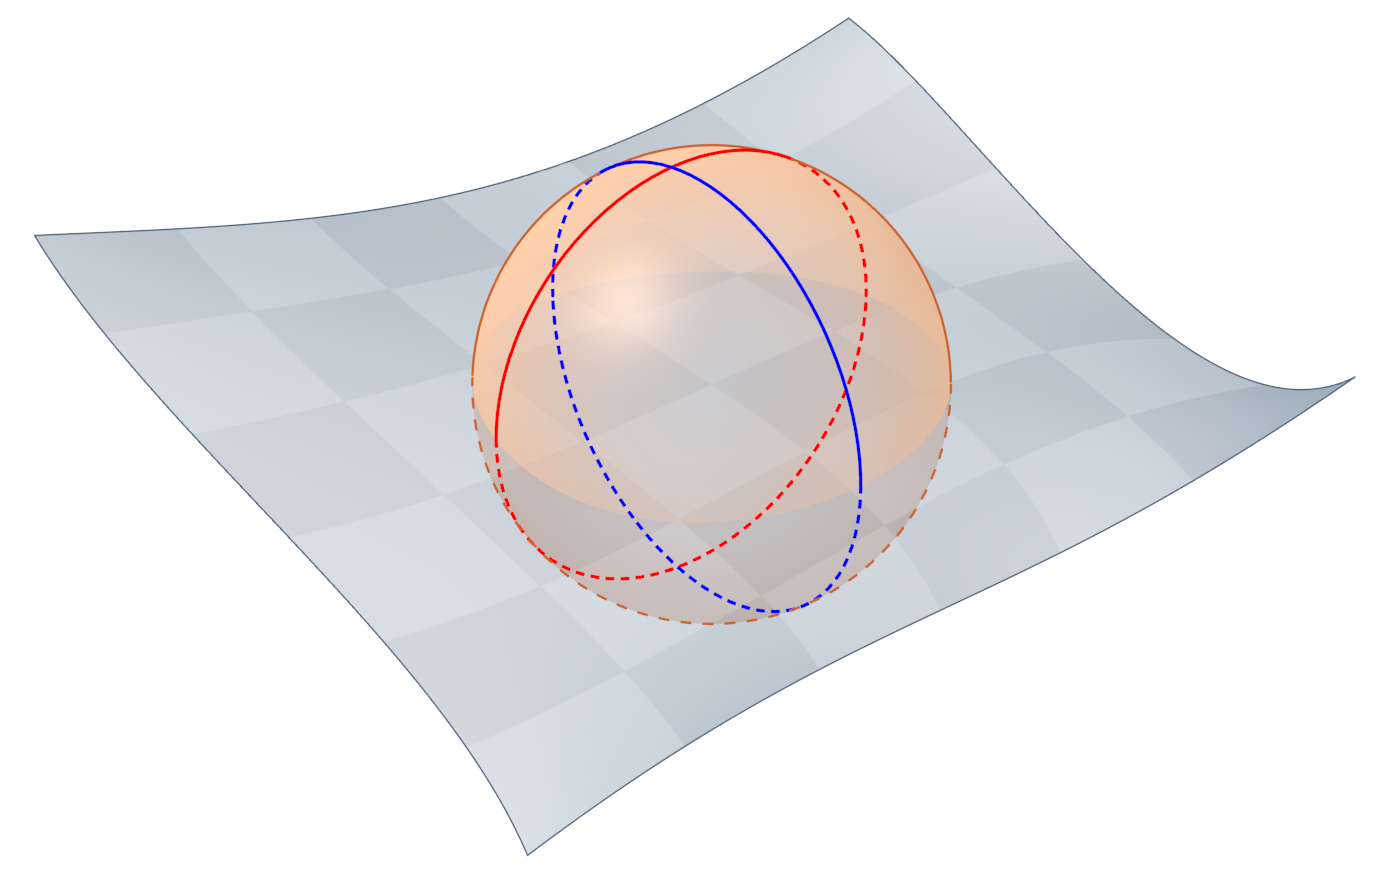
\includegraphics[width=\imagewidth]{figures/images/EdS_propre_carreau/EdS_propre_carreau.png}};
		%\drawGrid{10}{10}{black, thin, dotted}
		\DTLassign{dbsurfpoint}{1}{\spx=x, \spy=y}
		\coordinate (s) at (\spx, \spy);
		%
		\DTLassign{dbEdSpoints}{1}{\eppx=x, \eppy=y}
		\DTLassign{dbEdSpoints}{2}{\empx=x, \empy=y}
		\coordinate (ep) at (\eppx, \eppy);
		\coordinate (em) at (\empx, \empy);
		\node [anchor=north, txt, xshift=0pt, label] at (ep) {$\eos^+$};
		\node [anchor=south, txt, xshift=3pt, yshift=2pt, label] at (em) {$\eos^-$};
		%
		\DTLassign{dbsurfvectors}{1}{\sux=x, \suy=y}
		\coordinate (su) at (\sux, \suy);
		\draw [vector, red] (s) -- (su) node [below, xshift=-1pt, label, txt] {$\bsu$};
		%
		\DTLassign{dbsurfvectors}{2}{\svx=x, \svy=y}
		\coordinate (sv) at (\svx, \svy);
		\draw [vector, blue] (s) -- (sv) node [above, xshift=-5pt, label, txt] {$\bsv$};
		%
		\DTLassign{dbsurfvectors}{3}{\snx=x, \sny=y}
		\coordinate (sn) at (\snx, \sny);
		\draw [vector] (s) -- (sn) node [right, label, txt, black] {$\unv$};
		%
		\DTLassign{dbEdSnormals}{1}{\epnx=x, \epny=y}
		\coordinate (epn) at (\epnx, \epny);
		\node [anchor=west, label, txt, xshift=0pt] at (epn) {$\unv_{\envelope}^+$};
		\draw [dotted, thick, shorten >= 14pt] (s) -- (ep);
		\draw [vector] (ep) -- (epn);
		%
		\DTLassign{dbEdSnormals}{2}{\emnx=x, \emny=y}
		\coordinate (emn) at (\emnx, \emny);
		\node [anchor=west, label, txt, xshift=0pt] at (emn) {$\unv_{\envelope}^+$};
		\draw [dotted, thick, shorten <= 0pt, shorten >= 14pt] (s) -- (em);
		\draw [vector] (em) -- (emn);
		%
		\node [point] at (s) {};
		\node [point] at (ep) {};
		\node [point] at (em) {};
		%
		\node [anchor=east, txt, inner sep=2pt] at (s) {$\bs(u,v)$};
		\definecolor{colorSurfLabel}{rgb}{0.330, 0.413, 0.500}
		\node [txt, label, colorSurfLabel] at (0.1,0.68) {$\carreau$};
	\end{tikzpicture}
	\DTLgdeletedb{dbsurfpoint}%
	\DTLgdeletedb{dbsurfvectors}%
	\DTLgdeletedb{dbEdSpoints}%
	\DTLgdeletedb{dbEdSnormals}%
	\caption{Paramétrisation de l'EdS propre d'un carreau paramétrique.}
	\label{fig:EdS_propre_carreau}
\end{figure}

\begin{figure}
	\centering
	%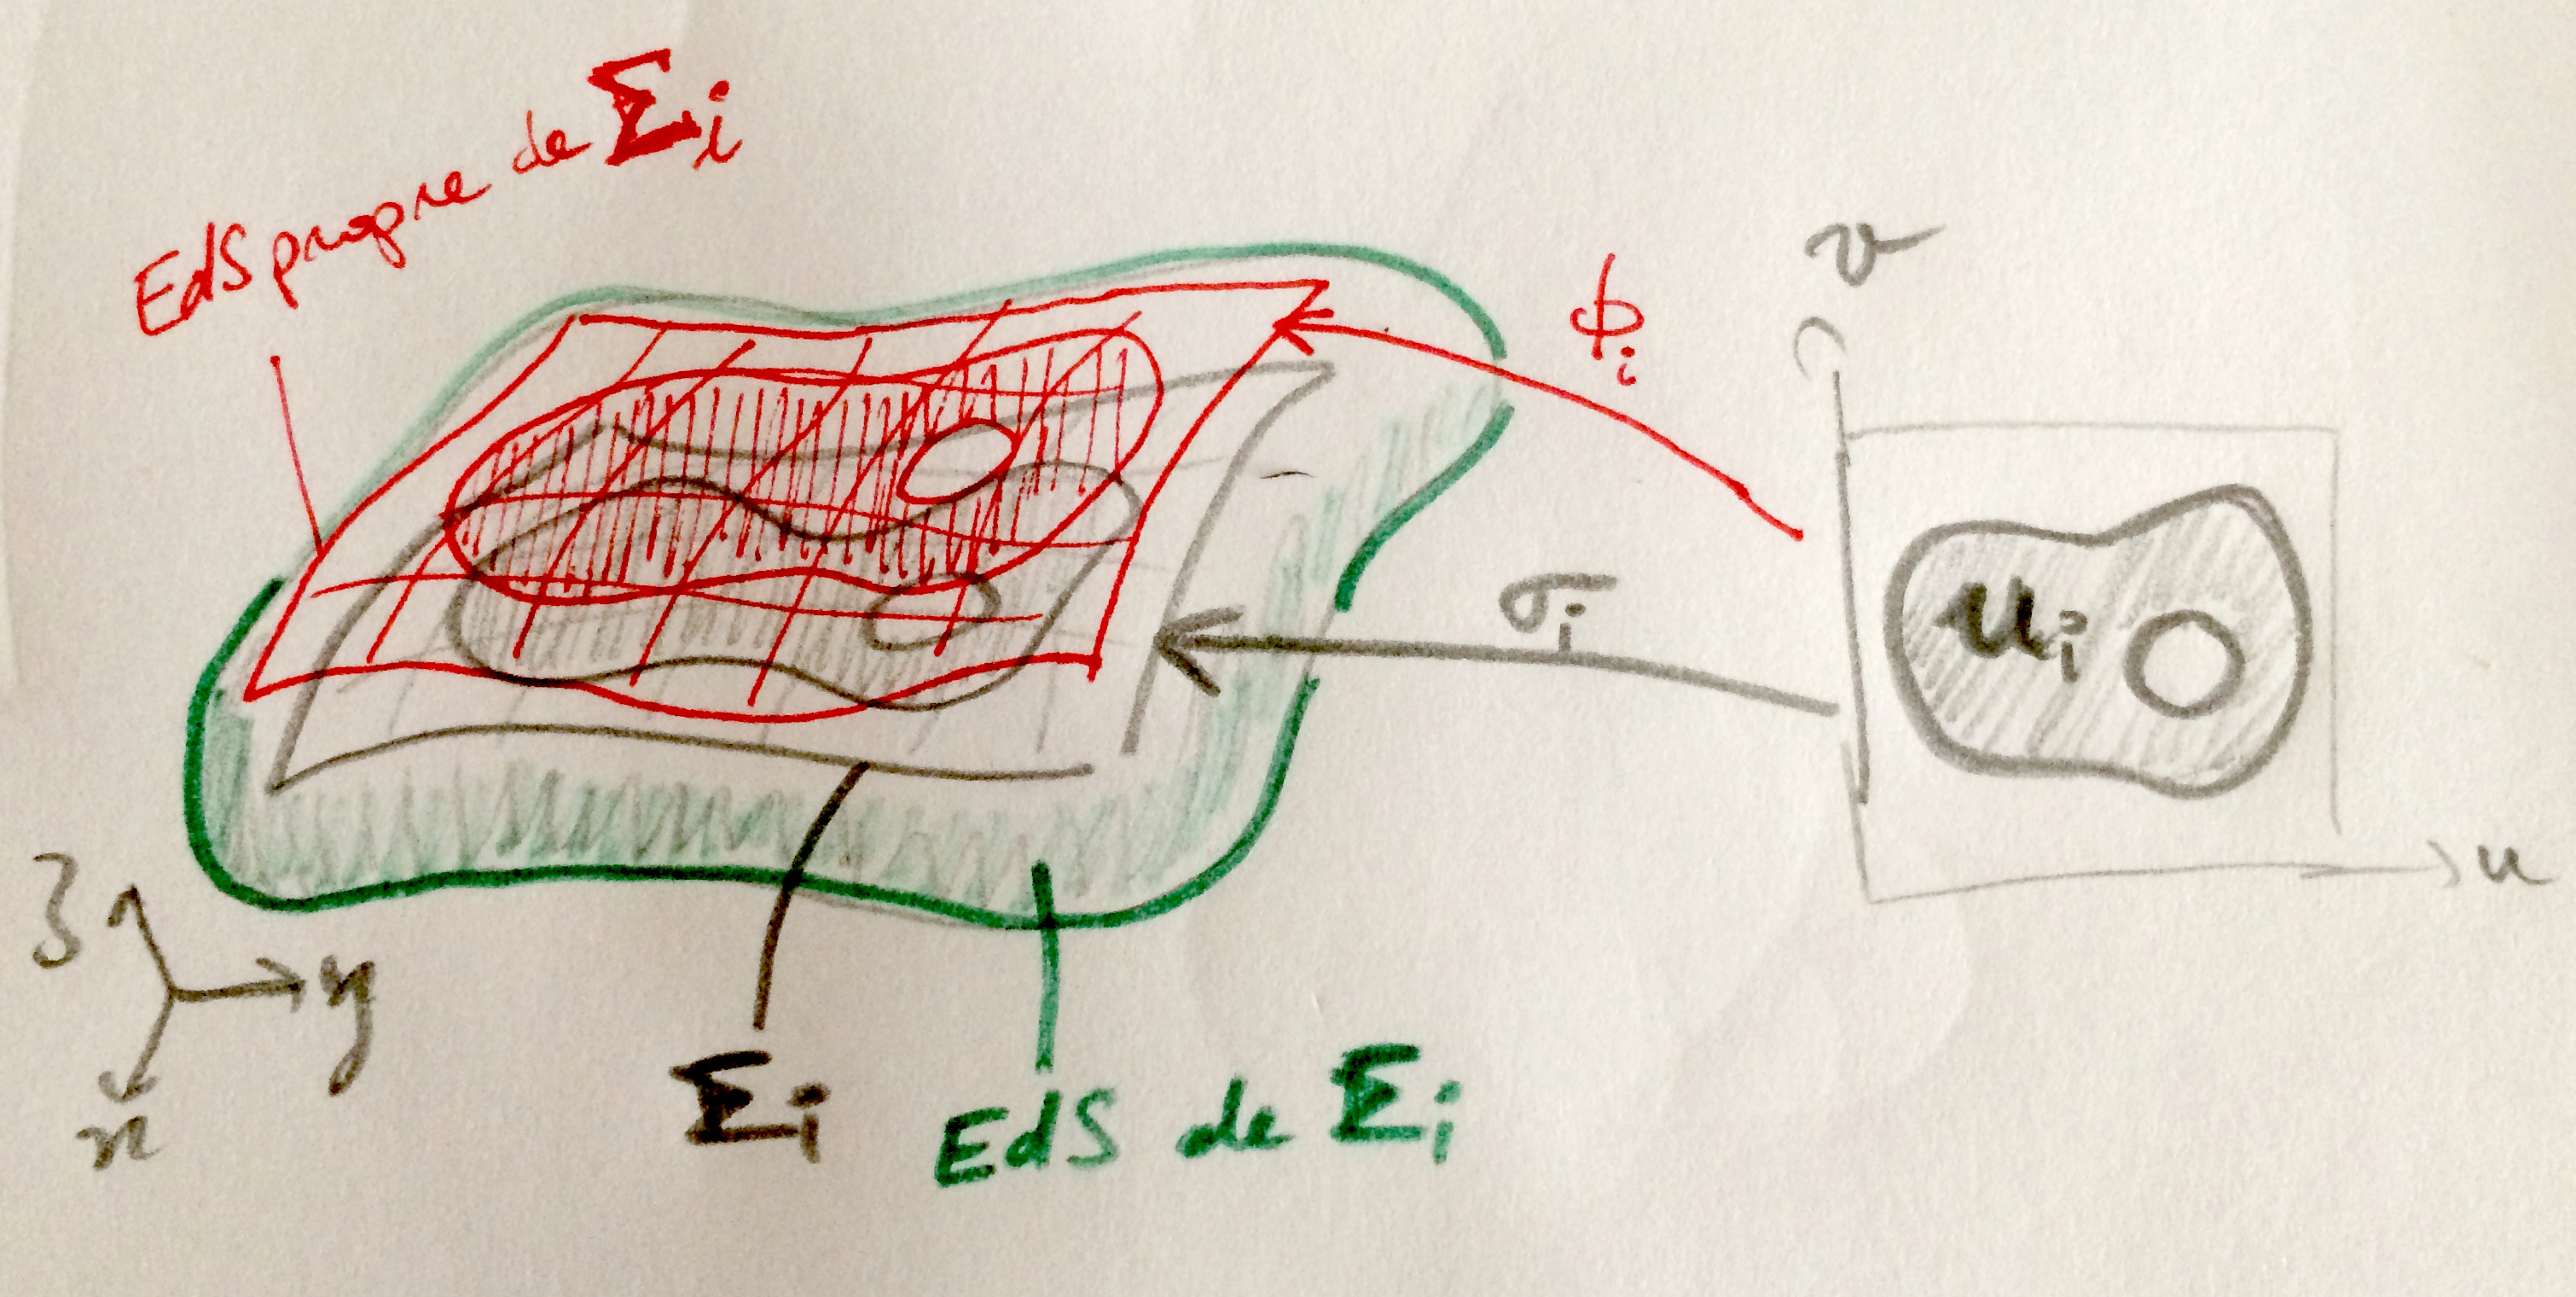
\includegraphics[width=10cm]{EdS_propre_carreau_restreint.JPG}
	\setlength{\imagewidth}{80mm}%
\setlength{\imageheight}{0.75\imagewidth}%
\definecolor{colorEdS}{HTML}{81BD3E}%
%\definecolor{colorInterieurDomaineUV}{HTML}{ADD9F4}%
%\definecolor{colorBordDomaineUV}{HTML}{6BA2BF}%
%\colorlet{colorInterieurDomaineUV}{mycolor_5}%
%\definecolor{colorInterieurDomaineUV}{RGB}{235, 220, 178}
\definecolor{colorInterieurDomaineUV}{HTML}{FFEED5}%
\colorlet{colorBordDomaineUV}{colorInterieurDomaineUV!70!black}%
\definecolor{colorFace0}{HTML}{6BA2BF}%
\definecolor{colorFace1}{HTML}{C25D53}%
\begin{tikzpicture}[
	img/.style={anchor=south west, inner sep=0},
	axe/.style={-stealth, line width=0.5pt},
	axelabel/.style={font=\small},
	axeuvlabel/.style={axelabel, inner sep=0},
	map/.style={
		shorten >= 2pt,
		-{Classical TikZ Rightarrow[length=4pt,width=4pt]}
	}
]
	\begin{scope}[
		x=\imagewidth,
		y=\imageheight
	]
		\node[img] (3dscene) {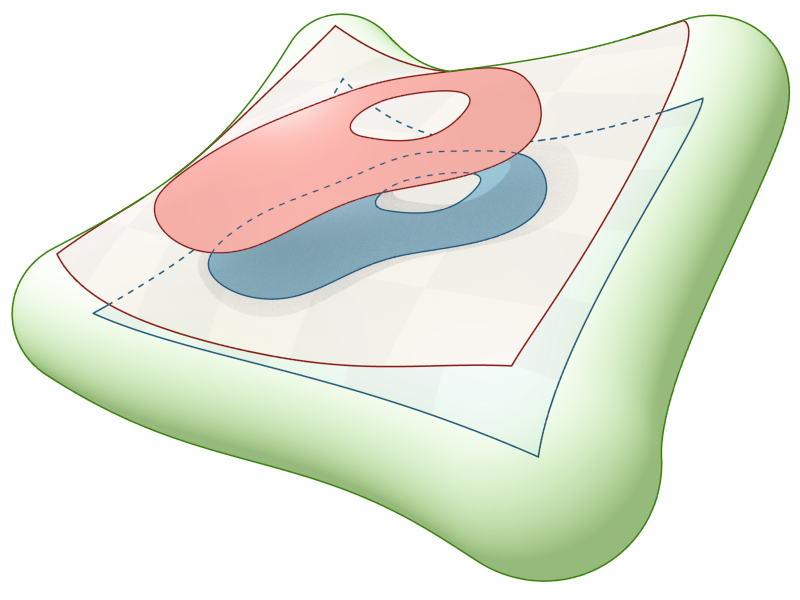
\includegraphics[width=80mm]{EdS_propre_carreau_restreint/EdS_propre_carreau_restreint.png}};
		%\drawGrid{20}{20}{blue, thin, dotted}%%%
		\node[colorFace0] at (0.64, 0.31) {$\carreau$};
		\node[colorFace1] at (0.57, 0.455) {$\EdSpropreplus{\carreau}{\rho}$};
		\node[colorFace0!50!black] at (0.35, 0.55) {$\brepface$};
		\node[colorFace1, anchor=south, inner sep=0] at (0.355, 0.695) {$\EdSpropreplus{\brepface}{\rho}$};
		\node[colorEdS, anchor=west] at (0.81, 0.1) {$\EdS{\carreau}{\rho}$};
		\coordinate (destMap0) at (0.55, 0.3);
		\coordinate (destMap1) at (0.4, 0.93);%(0.375, 0.9);
	\end{scope}
	%
	\begin{scope}[
		x=0.3\imageheight,
		y=0.3\imageheight,
		shift={(-0.5\imageheight,0.5\imageheight)}
	]
		{\transparent{0.035}%
			\drawUVchecker{6}{black}
		}%
		\path[draw=colorBordDomaineUV, fill=colorInterieurDomaineUV, line width=0.6pt]
(0.5265310634108271, 0.438547589973437) .. controls (0.3310295488391929, 0.6935604776607408) and (-0.021382588776948222, 0.7376543228644009) .. (-0.10761414246666436, 0.6458722526584881)
.. controls (-0.21738265636518123, 0.5288877287485011) and (-0.17017248387614453, 0.367245125596702) .. (-0.2879469981322148, 0.19968851382281255)
.. controls (-0.40569858776829065, 0.03213190204887557) and (-0.6468263047931714, -0.04383071753181846) .. (-0.693539828033049, -0.2425873818597733)
.. controls (-0.7509242728775373, -0.48485275979627296) and (-0.41538197233103924, -0.7039845421685414) .. (-0.15341941399581885, -0.6891054816069568)
.. controls (0.1085262173182571, -0.6742682161592514) and (0.16478678736946484, -0.4840377550744662) .. (0.3373277172510478, -0.34364796735972497)
.. controls (0.5098686471326309, -0.20327907720189958) and (0.9385113528049314, -0.09879129235910938) .. (0.5265310634108271, 0.438547589973437)
-- cycle
(0.42885638368115414, 0.1734202847133243) .. controls (0.4481705327582044, -0.06518802075369291) and (0.280929641274987, -0.06594033280456221) .. (0.16421795586878063, -0.05212704764834414)
.. controls (0.047447004991011434, -0.03833466004908937) and (0.03296990893768833, 0.11674611021456661) .. (0.08180520084194194, 0.20877895110413416)
.. controls (0.13056009984453748, 0.3008326895506175) and (0.40950330245547123, 0.4120494877373048) .. (0.42885638368115414, 0.1734202847133243)
-- cycle
;
		\node[colorBordDomaineUV] at (-0.2, -0.25) {$\uvdomain$};
		\draw[axe] (-1,-1) -- ++ (2.05,0) node [below right, axeuvlabel] {$u$};
		\draw[axe] (-1,-1) -- ++ (0,2.05) node [above left, axeuvlabel] {$v$};
		%
		\node[inner sep=0.3] (uvcenter) at (0,0) {};
		\draw[map, colorFace0] (1.05, -0.45) to [bend right=20] node[below] {$\bs$} (destMap0);
		\draw[map, colorFace1] (1.05, 0.45) to [bend left=20] node[above] {$\eos$} (destMap1);
	\end{scope}
\end{tikzpicture}
	\caption{EdS propre d'un carreau paramétrique restreint.}
	\label{fig:EdS_propre_carreau_restreint}
\end{figure}



\subsection{Paramétrisation de la pseudo-EdS d'une arête \brep\ convexe}% arc paramétrique}
%\begin{enumerate}
%	\item détermination de la convexité de l'arête (signe de $\dotprod{\left(\crossprod{\unv_L}{\unv_R}\right)}{\vrm{t}}$, \cf \autoref{section:def_convexite_courbe_singuliere})
%	\item rappeler système définissant une EdS propre à 1 paramètre
%	\item notion de cercle caractéristique
%	\item paramétrisation générique $\eos(u,v) = \vit{o}(u) + r(u)\vrm{r}(u,v)$ de l'EdS propre
%	\item restriction à la portion entre les EdS propres des faces incidentes, paramétrisée sur le domaine $\uvdomain = \left[ \lo{u}, \hi{u} \right] \times \left[ \lo{v}, \hi{v} \right]$
%\end{enumerate}

\subsubsection{Paramétrisation de l'EdS propre d'un arc paramétrique}
\label{section:parametrisation_EdS_propre_courbe}

\begin{figure}
	\centering
	\setlength{\imagewidth}{120mm}%
	\setlength{\imageheight}{0.6857\imagewidth}%
	\definecolor{coloreos}{HTML}{64CF36}
	\definecolor{colorshpere}{HTML}{CD6E33}
	\begin{tikzpicture}[x=\imagewidth, y=\imageheight]
		\node[inner sep=0, anchor=south west] {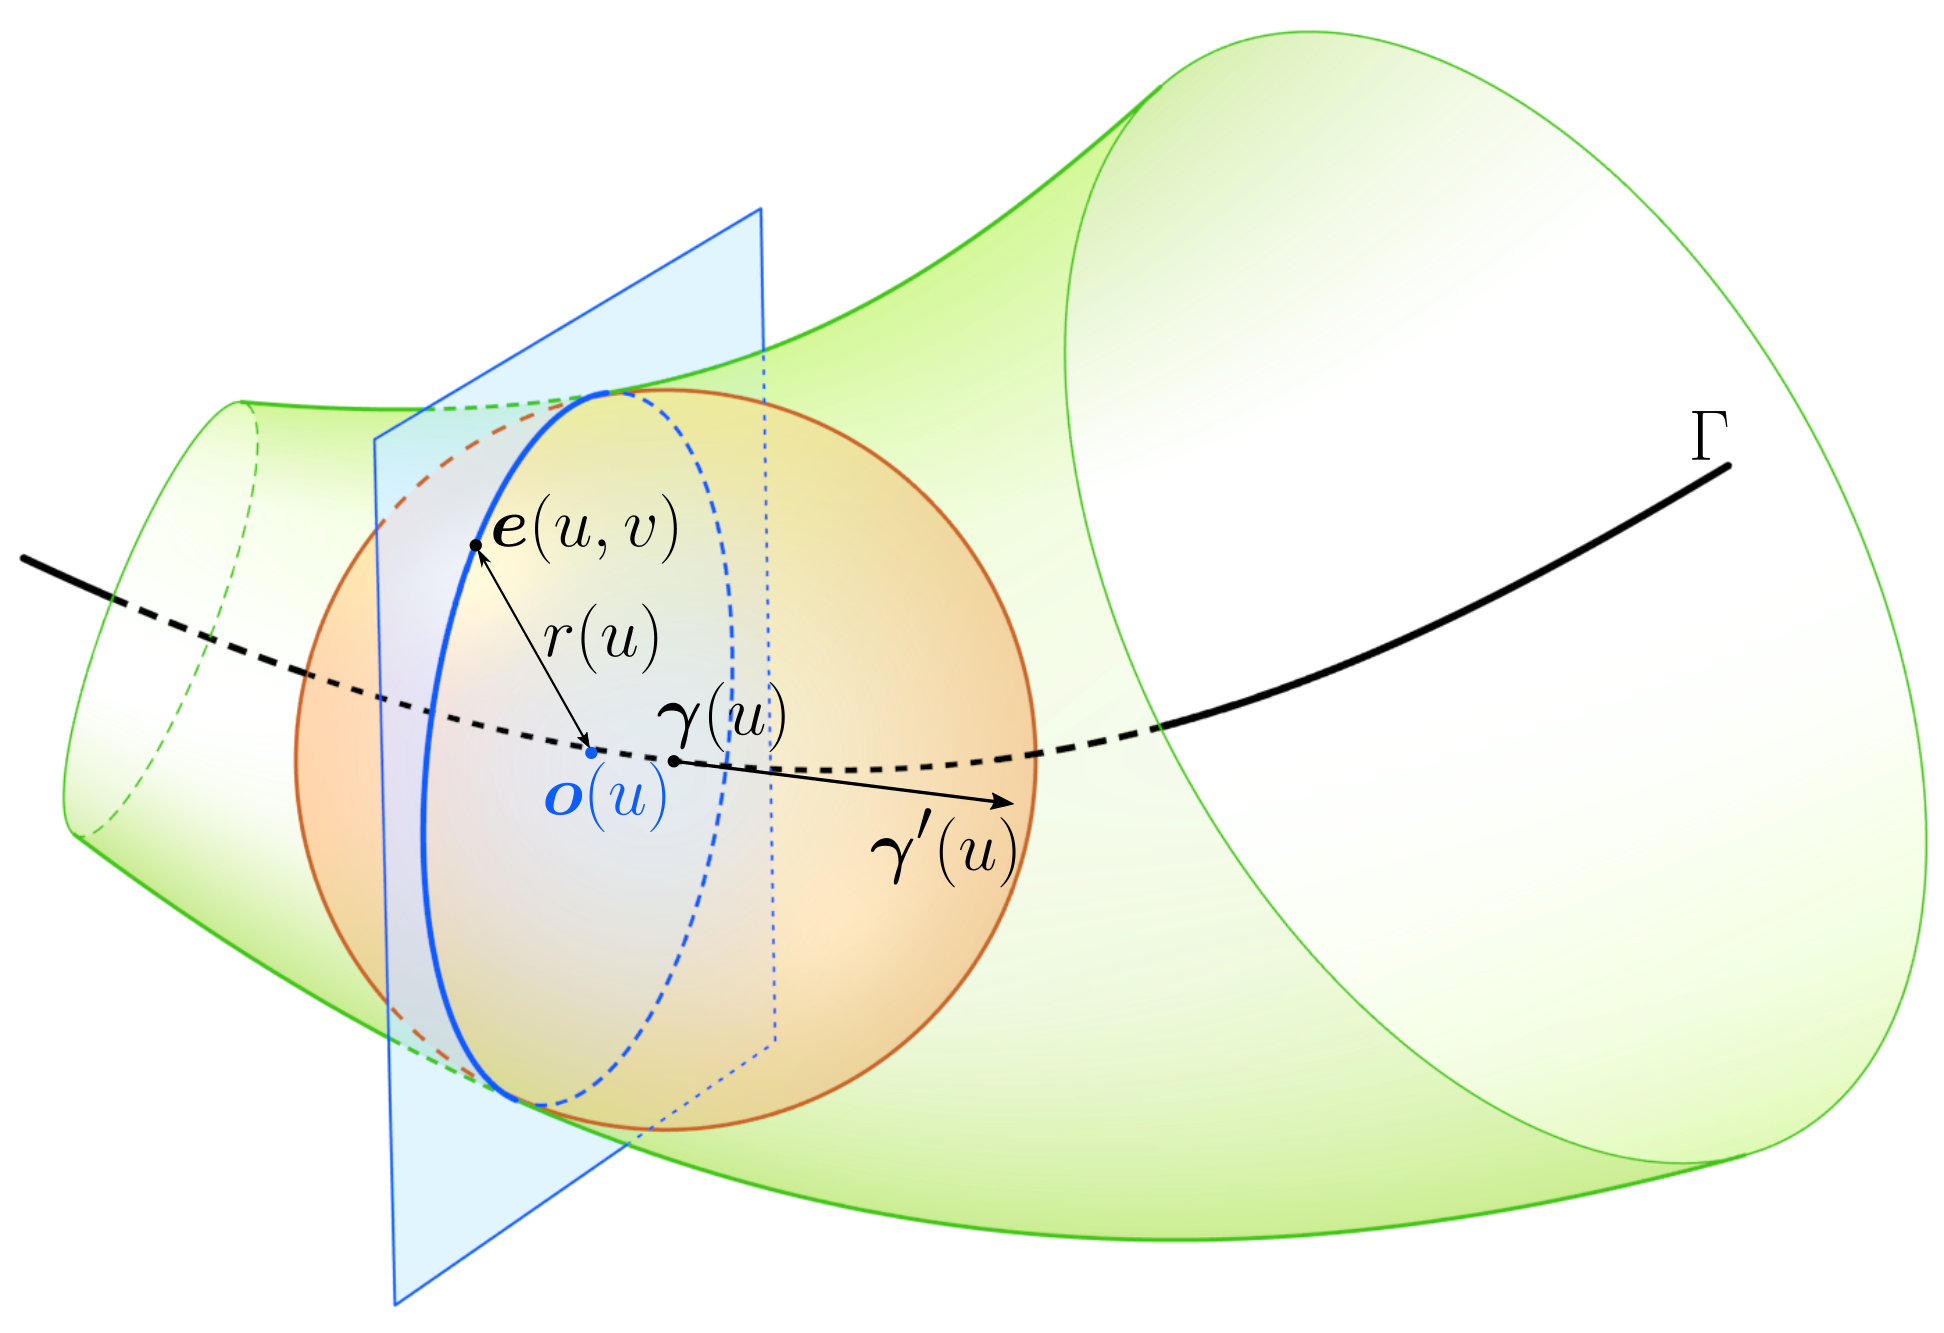
\includegraphics[width=\imagewidth]{figures/images/EdS_propre_courbe.png}};
		\node[coloreos] at (0.55,0.95) {$\EdSpropre{\Gamma}{\rho}$};
		\node[anchor=south west, colorshpere] at (0.46,0.62) {$\sphere[u]$};
	\end{tikzpicture}
	\caption{Paramétrisation de l'EdS propre d'un arc paramétrique.}
	\label{fig:parametrisation_EdS_propre_courbe}
\end{figure}
%%Soit $\bg : \wdomain \to \reals^3$ une paramétrisation du support géométrique $\Gamma$ de l'arête $\brepedge$. 
%%L'EdS propre de $\Gamma$ est le lieu des points $\bx \in \reals^3$ qui vérifient
%L'enveloppe $\Phi$ d'une famille de sphères à un paramètre centrées sur une courbe directrice $\Gamma$ est appelée \textit{surface canal} \cite{monge1850}. 
%Si la $\Gamma$ dispose d'une paramétrisation $\bg : \wdomain \to \reals^3$ alors cette surface est le lieu des points $\bx \in \reals^3$ qui vérifient
%\begin{equation}
%  \left\{
%    \begin{matrix}
%        \normtwo{\bx - \bg(u)}^2 - \rho(u)^2 &= 0 ,\\ 
%        \dotprod{\left(  \bx - \bg(u) \right)}{\bg'(u)} + \rho(u)\rho_u(u) &= 0.
%    \end{matrix}
%  \right.
%  \label{eq:sys_canal_surface}
%\end{equation}
Soit $\bg : \left[ \lo{u}, \hi{u} \right] \to \reals^3$ une paramétrisation du support géométrique $\Gamma$ de l'arête $\brepedge$. 
Si l'on considère $\rho$ comme une fonction du paramètre $u$ alors $\EdSpropre{\Gamma}{\rho}$ est le lieu des points $\bx \in \reals^3$ qui vérifient
\begin{equation}
  \left\{
    \begin{matrix}
        \normtwo{\bx - \bg(u)}^2 - \rho(u)^2 &= 0 ,\\ 
        \dotprod{\left(  \bx - \bg(u) \right)}{\bg'(u)} + \rho(u)\rho_u(u) &= 0.
    \end{matrix}
  \right.
  \label{eq:sys_canal_surface}
\end{equation}
A condition que $\rho_u^2 \leq \normtwo{\bg'}^2$, le système \eqref{eq:sys_canal_surface} définit une famille de \textit{cercles caractéristiques}, dont chacun est le lieu des points de tangence entre $\EdSpropre{\Gamma}{\rho}$ et une sphère de la famille $\sphere[\Gamma][\rho]$ (voir \autoref{fig:parametrisation_EdS_propre_courbe}).
\par
D'après \eqref{eq:sys_canal_surface}, le cercle caractéristique au point $\bg(u)$ est l'intersection de la sphère $\sphere[u] = \sphere[\bg(u)][\rho(\bg(u))]$ et d'un plan orthogonal à la tangente à $\Gamma$ en ce point (donnée par le vecteur $\bg'(u)$). 
Ce cercle est centré en
\begin{equation}
    \vit{o}(u) = \bg(u) - \frac{\rho(u)\rho_u(u)}{\normtwo{\bg'(u)}^2} \bg'(u),
    \label{eq:cercle_caracteristique_centre}
\end{equation}
et a pour rayon
\begin{equation}
    r(u) = \rho(u) \sqrt{1 - \frac{\rho_u(u)^2}{\normtwo{\bg'(u)}^2}}.
    \label{eq:cercle_caracteristique_rayon}
\end{equation}
\par
Voir $\EdSpropre{\Gamma}{\rho}$ comme une famille cercles caractéristiques permet d'en donner la paramétrisation suivante
\begin{equation}
    \eos(u,v) = \vit{o}(u) + r(u)\vrm{r}(u,v),
    \label{eq:parametrisation_EdS_propre_courbe}
\end{equation}
où $\vrm{r}$ vérifie
\begin{equation}
	\left\{
		\begin{matrix}
			\normtwo{\vrm{r}} = 1,\\ 
			\dotprod{\vrm{r}}{\bg'} = 0.
		\end{matrix}
	\right.
\end{equation}
De cette façon, les courbes iso-$u$ de $\eos$ sont les cercles caractéristiques.


\subsubsection{Paramétrisation de la pseudo-EdS}
\label{section:parametrisation_pseudo_EdS_arete}
\newcommand{\eosR}{\lo{\vit{\eos}}}
\newcommand{\eosL}{\hi{\vit{\eos}}}

\newcommand{\psiR}{\lo{\vit{\psi}}}
\newcommand{\psiL}{\hi{\vit{\psi}}}


\begin{figure}
    \centering
    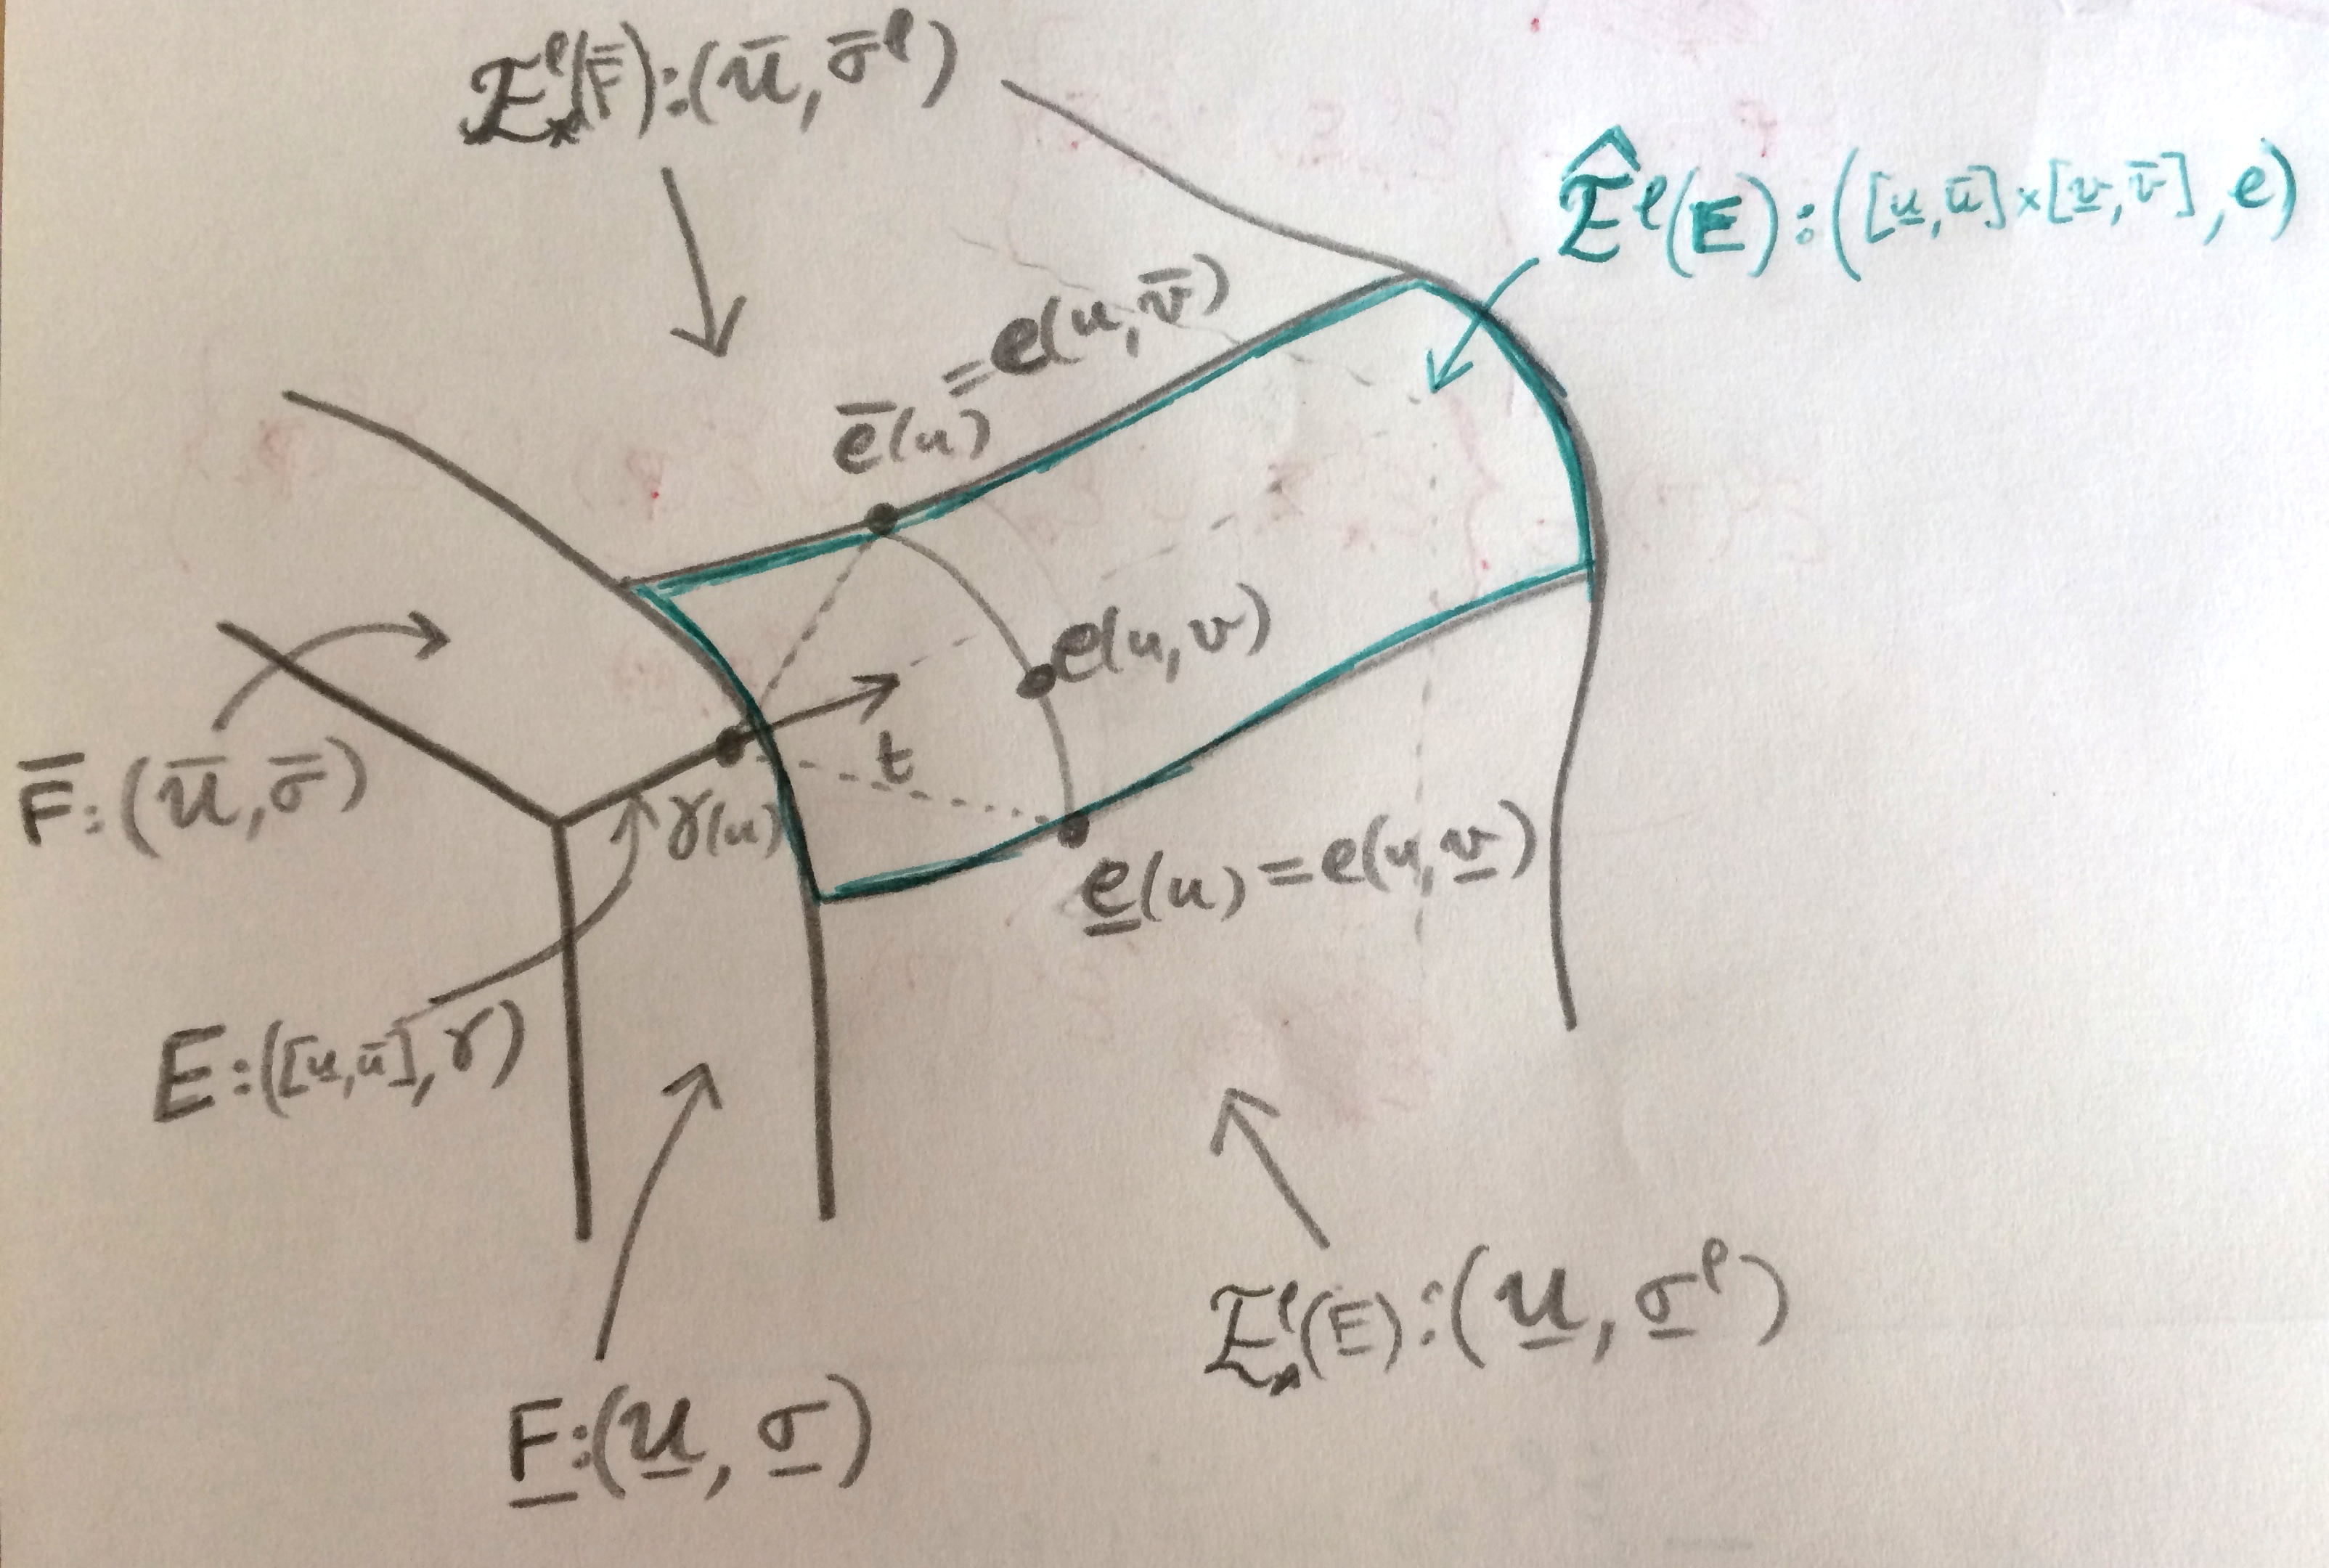
\includegraphics[width=10cm]{pseudo-EdS_arete.JPG}
    \caption{Paramétrisation de $\pseudoEdS{\brepedge}{\rho}$}
    \label{fig:pseudo-EdS_arete}
\end{figure}






\subsection{Paramétrisation de la pseudo-EdS d'un sommet \brep\ convexe}
2 approches :

\subsubsection{Polygone sphérique découpé en quadrilatères}
\label{section:quadrangulation_polygone_spherique}
avantages/inconvénients :
\begin{itemize}
	\item[$-$] valable seulement si la vitesse normale est uniforme
	\item[$-$] génère plusieurs nouveaux carreaux de surface
	\item[$+$] les nouveaux carreaux sont rectangulaires ($\Rightarrow$ permet l'utilisation de quadratures simples (\cf \autoref{section:clenshaw_curtis_quadrature})
\end{itemize}


\subsubsection{Ajustement de carreau sphérique à un nuage de points}
\label{section:ajustement_carreau_spherique}

\def\s{\vit{s}}

%(\cf notes Huygens)
avantages/inconvénients :
\begin{itemize}
	\item[$-$] le nouveau carreau est restreint
	\item[$+$] valable également si la vitesse normale varie spatialement
	\item[$+$] génère un seul nouveau carreau de surface
\end{itemize}

Soit $\brepvertex$ un sommet \brep\ convexe dont le support géométrique est le point $\p$. 
On cherche à construire un carreau paramétrique restreint décrivant $\pseudoEdS{\p}{\rho}$ \ie la région de la sphère $\sphere[\p][\rho{\p}]$ délimitée par les arcs de cercles caractéristiques aux extrémités des arêtes \brep\ incidentes à $\p$. 
Afin de simplifier cette construction, on considère que $\p$ est situé à l'origine et que $\rho(\p) = 1$. 
(On appliquera la transformation adéquate en fin de construction pour se placer à nouveau dans le cas général.)
\par
Le problème consiste alors, étant donné un ensemble de points $S = \family{\s}{i}{1}{n}$ sur la sphère unité $\mathbb{S}^2$, à construire un carreau paramétrique décrivant une portion $R$ de $\mathbb{S}^2$ contenant $S$. 
On cherche également à minimiser l'aire de $R$ \ldots




\section{Construction d'un modèle \brep\ de l'EdB}

\subsection{Construction du graphe des intersections}
Conservation/création des intersections tangentielles, calcul des intersections transverses entre paire de carreaux non-restreints, segmentation des courbes d'intersection en segments quasi-disjoints (intersection de 3 carreaux non-restreints ou plus), \guillemets{clipping} par le domaine paramétrique de chaque carreau restreint
\par\bigskip
pour un carreau de surface, il s'agit d'un graphe planaire orienté dont un plongement dans $\reals^2$ est donné par la trace des courbes d'intersections dans son espace paramétrique

\begin{figure}
	\centering
	\plotCurvedDirectedGraph{/d/bandrieu/GitHub/FFTsurf/test/graph/graph_bezier_control_points.dat}{25mm}
	\caption{Plongement du graphe des intersections dans l'espace paramétrique d'un carreau de surface.}
\end{figure}


\subsection{Construction des faces, arêtes et sommets \brep}
pour chaque carreau : extraction des cycles du graphe d'intersection, caractérisations des contours (extérieurs/intérieurs), détermination des faces $\to$ insertion des contours dans la \brep\ $\to$ insertion des (co-)arêtes et sommets
\begin{figure}
	\centering
	\newcommand{\arc}{\mathcal{A}}%
\newcommand{\subin}{\ensuremath{_{\mathrm{in}}}}%
\newcommand{\subout}{\ensuremath{_{\mathrm{out}}}}%
\newcommand{\noeud}{\mathcal{N}}%
\newcommand{\cycle}{\mathcal{C}}%
\newcommand{\graph}{\mathcal{G}}%
\begin{tikzpicture}[%
	scale=0.5,
	>={Latex[length=4pt]},      % Arrow style
    start chain=going below,    % General flow is top-to-bottom
    node distance=6mm and 50mm, % Global setup of box spacing
    every join/.style={flow},   % Default linetype for connecting boxes
    ]
% ------------------------------------------------- 
% A few box styles 
% <on chain> *and* <on grid> reduce the need for manual relative
% positioning of nodes
\tikzset{
  base/.style={draw, on chain, on grid, align=center, minimum height=4ex, minimum width=5em},
  proc/.style={base, rectangle},
  test/.style={base, diamond, aspect=2},
  term/.style={proc, rounded corners=2ex},
  % coord node style is used for placing corners of connecting lines
  coord/.style={coordinate, on chain, on grid, node distance=6mm and 25mm},
  % -------------------------------------------------
  % Connector line styles for different parts of the diagram
  flow/.style={->, draw}
}
% -------------------------------------------------
\node [term, join] (start) {Début};
\node [proc, join] (p1) {Éliminer les branches pendantes de $\graph$};
\node [test, join] (t1) {$A = \emptyset$ ?};

\node [proc] (startarc) {Choisir un arc $\arc_*$ de $\graph$};

\node [proc, join] {Démarrer un nouveau cycle $\cycle$ à partir de $\arc_*$};
\node [proc, join] {$\arc \leftarrow \arc_*$ et\\ $\noeud \leftarrow \dest(\arc)$};


\node [test, join] (t2) {$\noeud = \orig(\arc_*)$?};

\node [proc] (maxangles) {Identifier $\hi{\alpha}\subin$, $\hi{\alpha}\subout$ et $\hi{\arc}\subout$};


\node [test, join] (t3) {$\hi{\alpha}\subin > \hi{\alpha}\subout$ ?};
\node [proc] (abortcycle) {Abandonner $\cycle$};

\node [term, left=of t1, text width=3em] (end) {Fin};
\node [proc, right=of t2] (completecycle) {Rajouter $\cycle$\\à la liste des cycles\\et l'extraire de $\graph$};
\node [proc, left=of t3] (appendcycle) {$\arc \leftarrow \hi{\arc}\subout$,\\ $\noeud \leftarrow \dest(\arc)$ et \\ajouter $\arc$ à $\cycle$};


\draw [flow] (t1.west) -- node[above] {oui} (end);
\draw [flow] (t1.south) -- node[left] {non} (startarc);

\draw [flow] (t2.east) -- node[above] {oui} (completecycle);
\draw [flow] (t2.south) -- node[left] {non} (maxangles);

\draw [flow] (t3.west) -- node[above] {oui} (appendcycle);
\draw [flow] (t3.south) -- node[left] {non} (abortcycle);


\draw [flow] (appendcycle.north) |- (t2);

\node [coord, left=of appendcycle] (c2)  {};
\draw [flow] (abortcycle.west) -| (c2) |- (p1);

\draw [flow] (completecycle.north) |- (p1);
% -------------------------------------------------
\end{tikzpicture}
	\caption{Organigramme de l'algorithme d'extraction des cycles d'un graphe orienté plongé dans $\reals^2$.}
\end{figure}


\begin{figure}
	\centering
	\setlength{\imagewidth}{60mm}%
\setlength{\imageheight}{\imagewidth}%
%
\colorlet{facecolor1}{mycolor_1}
\colorlet{facecolor2}{mycolor_2}
\colorlet{facecolor3}{mycolor_3}
%
\begin{tikzpicture}[
	x=0.5\imagewidth, 
	y=0.5\imageheight,
	halfedge/.style={
		line width=0.8pt, 
		line cap=round, 
		-{Triangle[left]}
	},
]
	%\input{/d/bandrieu/GitHub/FFTsurf/test/graph/graph_faces_tikzcode.tex}
	\input{../../FFTsurf/test/graph/graph_faces_tikzcode.tex}
\end{tikzpicture}

	\caption{Faces du graphe}
\end{figure}

\chapter{Mise en \oe uvre numérique de l'algorithme de propagation}
\label{chap:methode_numerique}

Dans ce chapitre, on propose une mise en \oe uvre numérique de l'algorithme présenté au chapitre précédent. 
\begin{enumerate}
	\item choix de la discrétisation spatiale
	\begin{itemize}
		\item représentation des carreaux de surface
		\item représentation (et calcul) des courbes d'intersection entre carreaux
	\end{itemize}
	\item intégration temporelle
	\begin{itemize}
		\item intégration explicite du champ de vitesse 
		\item construction géométrique discrète de l'EdB suivant une méthode pseudo-spectrale (exacte aux points de collocation + interpolation)
	\end{itemize}
	\item considérations sur la stabilité numérique
\end{enumerate}



%\section{Discrétisation (pseudo-)spectrale en espace}
\section{Représentation des carreaux de surface}
\subsection{État de l'art}
\begin{enumerate}
	\item harmoniques sphériques \cite{rahimian2015}
	\item polynômes trigonométriques \cite{gueyffier2015}
	\item[$\Rightarrow$] limitations géométriques (régularité globale) et topologique (périodicité)
	\item modèle \brep\ permet une plus grande flexibilité
	\item polynômes algébriques (en produit tensoriel) adaptés aux carreaux de surface
	\item CAO : Bezier, NURBS $\to$ base des polynômes de Bernstein
	\begin{itemize}
		\item $B_n^N(x) = \binom{N}{n} \left( 1 - x \right)^{N-n} x^n$ pour $0 \leq n \leq N$.
		\item positivité : pour $0 \leq x \leq 1$, $B_n^N(x) \geq 0$
		\item partition de l'unité : $\sum_{n = 0}^N B_n^N = 1$
		\item[$\to$] propriétés intéressantes pour la conception géométrique
		\begin{itemize}
			\item coefficients = points de contrôle
			\item l'enveloppe convexe des points de contrôle englobe la courbe/surface de Bézier
		\end{itemize}
		\item inconvénients :
		\begin{itemize}
			\item points de contrôle pas \emph{sur} la courbe/surface $\Rightarrow$ pas exploitables comme marqueurs lagrangiens
			\item algorithme d'évaluation (de Casteljau) numériquement stable mais coûteux $\bigO{N^2}$
		\end{itemize}
	\end{itemize}
	\item motivation le choix des polynômes de Chebyshev
\end{enumerate}

%\subsection{Polynômes de Bernstein}
%Les polynômes de Bernstein sont définis par
%\begin{equation}
%	B_n^N(x) = \binom{N}{n} \left( 1 - x \right)^{N-n} x^n,
%	\label{eq:bernstein_poly}
%\end{equation}
%pour $0 \leq n \leq N$.
%Propriétés :
%\begin{itemize}
%	\item positivité : pour $0 \leq x \leq 1$, $B_n^N(x) \geq 0$
%	\item partition de l'unité : $\sum_{n = 0}^N B_n^N = 1$
%	\item dérivée : ${B_n^N}' = N \left( B_{n-1}^{N-1} - B_n^{N-1} \right)$
%\end{itemize}
%Avantages/inconvénients
%\begin{itemize}
%	\item[$+$] coefficients = points de contrôle dans l'espace physique, sens géométrique intuitif
%	\item[$+$] partition de l'unité sur $\berninterval$ $\Rightarrow$ propriété d'enveloppe convexe
%	\item[$\pm$] algorithme d'évaluation (de Casteljau) numériquement stable mais coûteux $\bigO{N^2}$
%	\item[$-$] points de contrôle pas \emph{sur} la courbe/surface $\Rightarrow$ pas exploitables comme marqueurs lagrangiens
%	\item[$-$] peu pratiques pour réduire/élever le degré des polynômes
%\end{itemize}


\subsection{Polynômes de Chebyshev univariés}
Les polynômes de Chebyshev sont très largement utilisés dans de nombreux domaines tels que l'analyse numérique.
L'objet des sections suivantes est de rappeler la définition de cette famille de polynômes et d'en présenter brièvement les propriétés remarquables qui seront exploitées dans cette thèse. 
Nombreux sont les ouvrages consacrés aux polynômes de Chebyshev \cite{mason2002, gil2007} ainsi qu'à leur usage dans les méthodes spectrales \cite{boyd2001, canuto2006}, aussi le lecteur est invité à s'y référer pour plus de détails.

\subsubsection{Définition et principales propriétés}
\begin{definition}
	Pour $n \in \mathbb{N}$, le polynôme de Chebyshev (de première espèce) $T_n$ est défini par%un polynome de degré $n$ défini par
	\begin{equation}
		T_n(\cos \theta) = n \cos \theta.
		\label{eq:chebyshev_trigo}
	\end{equation}
\end{definition}
%De la définition \eqref{eq:chebyshev_trigo} et de l'identité trigonométrique
De cette définition et de l'identité trigonométrique $\cos n\theta + \cos (n-2)\theta = 2\cos \theta \cos (n-1)\theta$, on peut déduire la relation de récurrence suivante, pour $-1 \leq x \leq 1$, 
\begin{align}[left = \empheqlbrace\,]
	T_0(x) &= 1, \nonumber\\
	T_1(x) &= x, \nonumber\\
	T_n(x) &= 2x T_{n-1}(x) - T_{n-2}(x) \text{,\ pour\ } n \geq 2.
	\label{eq:chebyshev_recurrence}
\end{align}
Le graphe des six premiers polynômes de Chebyshev est tracé sur la \autoref{fig:chebyshev_polynomials}.\par

\begin{figure}
	\centering
	%https://tex.stackexchange.com/questions/127375/replicate-the-fourier-transform-time-frequency-domains-correspondence-illustrati
\begin{tikzpicture}[%
		ax/.style={on layer=background, black, line width=0.5pt},
		grid/.style={on layer=background, black!25, line width=0.4pt},
		tickl/.style={font=\small},
		myax/.style={}
	]%
	\begin{axis}[
	width=12cm, height=9cm,
    set layers=standard,
    %domain=-1:1,
    xmin=-1, xmax=1,
    zmin=-1, zmax=1,
    samples y=1,
    view={40}{30},
    %hide axis,
    axis line style={draw=none},
    tick style={draw=none},
    grid = none,
    axis lines* = left,
    unit vector ratio*=4 3 1,
    %xtick=\empty, ytick=\empty, ztick=\empty,
    xtick={-1,-0.5,0,0.5,1},
    ytick={0,1,2,3,4,5},
    ztick={-1,0,1},
    %xlabel={$x$},
    %ylabel={$n$},
    %zlabel={$T_n(x)$},
    yticklabels=\empty,
    %zticklabels=\empty,
    no marks,
    samples=201,
    every tick label/.append style={font=\small},
    %tick align=outside,
%    cycle list/GnBu-9,%RdYlBu-6,%Spectral-6,
%	cycle multiindex* list={GnBu-9},%RdYlBu-6}%Spectral-6}
    clip=false
]
% x,z grid lines (at y=cst)
\foreach \y in {0,1,...,5}{%
	\foreach \x in {{-0.5},{0},{0.5},{1}}{
		\begingroup\edef\temp{\endgroup\noexpand\draw [grid] (axis cs:\x,\y,-1) -- ++ (axis direction cs:0,0,2);}\temp
	}
	\foreach \z in {{0},{1}}{
		\begingroup\edef\temp{\endgroup\noexpand\draw [grid] (axis cs:-1,\y,\z) -- ++ (axis direction cs:2,0,0,0);}\temp
	}
}
\pgfplotsinvokeforeach{0,1,...,5}{%
	\addplot3+[domain=-1:1]	({x},#1,{ cos(#1*acos(x)) });
%	\node[font=\footnotesize, anchor=west, inner sep=0] 
%		at (axis cs:1,#1,-0.3) {$n = #1$};
	\draw [ax] (axis cs:-1,#1,-1) -- ++ (axis direction cs:2,0,0); % x-axis
	\draw [ax] (axis cs:-1,#1,-1) -- ++ (axis direction cs:0,0,2); % z-axis
}%
% x,z ticks
\foreach \y in {0,1,...,5}{%
	\foreach \x in {{-1},{-0.5},{0},{0.5},{1}}{
		\begingroup\edef\temp{\endgroup\noexpand\draw [ax] (axis cs:\x,\y,-1) -- ++ (axis direction cs:0,0,0.2);}\temp
	}
	\foreach \z in {{-1},{0},{1}}{
		\begingroup\edef\temp{\endgroup\noexpand\draw [ax] (axis cs:-1,\y,\z) -- ++ (axis direction cs:0.05,0,0,0);}\temp
	}
}
% x, z tick labels and grid lines
%\pgfplotsinvokeforeach{-1,-0.5,0,0.5,1}{
%	\node[anchor=north, myax, tickl, xshift=-4pt] at (axis cs:#1,0,-1.1) {$#1$};
%%	\draw [grid] (axis cs:#1,0,-1) -- ++ (axis direction cs:0,5,0);
%}
%\pgfplotsinvokeforeach{-1,0,1}{
%	\node[anchor=east, myax, tickl] at (axis cs:-1,0,#1) {$#1$};
%%	\draw [grid] (axis cs:-1,0,#1) -- ++ (axis direction cs:0,5,0);
%}
% x,z labels
\node[anchor=north west, myax] at (axis cs:0,-1.1,-1) {$x$};
\node[anchor=south, rotate=90, myax, inner sep=7mm] at (axis cs:-1,0,0) {$T_n(x)$};
%
% y axis
\draw[ax, -latex] (axis cs:1.25,0,-1) -- ++ (axis direction cs:0,5.5,0) node[anchor=south west] {$n$};
\pgfplotsinvokeforeach{0,1,...,5}{%
	\draw[ax] (axis cs:1.25,#1,-1) -- ++ (axis direction cs:-0.05,0,0);
	\node[anchor=north west, myax, tickl] at (axis cs:1.25,#1,-1) {$#1$};
}
%\foreach \n in {0,1,...,5}{%
%	\node[font=\footnotesize, anchor=west, inner sep=0] 
%		at (axis cs:1,\n,-0.3) {$n = \n$};
%	\draw [ax] (axis cs:-1,\n,-1) -- ++ (axis direction cs:2,0,0); % x-axis
%	\draw [ax] (axis cs:-1,\n,-1) -- ++ (axis direction cs:0,0,2); % z-axis
%	\foreach \z in {-1,0,1}{%
%		\draw [ax] (axis cs:-1,\n,\z) -- ++ (axis direction cs:0.025,0,0);
%	}%
%	\foreach \x in {-1,-0.5,0,0.5,1}{%
%		\draw [ax] (axis cs:\x,\n,-1) -- ++ (axis direction cs:0,0,0.1);
%	}%
%}%
\end{axis}
\end{tikzpicture}
	\caption{Graphe des six premiers polynômes de Chebyshev.}% $(n=0,\ldots,5)$ sur l'intervalle $\chebinterval$.}
	\label{fig:chebyshev_polynomials}
\end{figure}

$T_n$ est un polynôme de degré $n$ %de coefficient dominant $2^{n-1}$ 
qui atteint ses extrema locaux sur $\chebinterval$ aux $n+1$ n\oe uds de Chebyshev-Gauss-Lobatto (CGL)%\footnote{Seuls les $n-1$ n\oe uds intérieurs sont réellement des extrema au sens où la dérivée s'y annule. A noter également que ces n\oe uds sont rangés en ordre décroissant.}
\begin{equation}
	x_k = \cos \frac{k \pi}{n},
	\label{eq:cgl_nodes}
\end{equation}
pour $0 \leq k \leq n$. 
Seuls les $n-1$ n\oe uds intérieurs sont réellement des extrema au sens où la dérivée s'y annule. 
À noter également que ces n\oe uds sont rangés en ordre décroissant.\par

\begin{figure}
	\centering
	\begin{tikzpicture} 
	\begin{axis}[%
		width=8cm, height=6cm,
		axis lines*=left,
		xmin=-1.0, xmax=1.0, ymin=-1.0, ymax=1.0,
		grid=major,
		clip marker paths=false,
		enlargelimits={abs=0.05},
		]%
		\addplot+[samples=200, domain=0:pi, no marks, mycolor_6] ({cos(deg(x))}, {cos(5*deg(x))});%
		% extrema
		\addplot+[samples=6, domain=0:pi, ycomb, dashed, mark=none, black] ({cos(deg(x))}, {cos(5*deg(x))});%
		\addplot+[samples=6, domain=0:pi, only marks, mark=*, black] ({cos(deg(x))}, {0});%
		% zeros
%		\pgfplotsinvokeforeach{0,...,4}{
%			\addplot+[mark=*, red] coordinates {(cos((2.0*#1+1.0)*180.0/10.0),0)};
%		}
	\end{axis} 
\end{tikzpicture}
%	\caption{N\oe uds de Chebyshev-Gauss-Lobatto pour $n = 6$ (extrema locaux du polynome $T_6$ sur l'intervalle $\chebinterval$).}
	\caption{N\oe uds de Chebyshev-Gauss-Lobatto (extrema locaux) du polynôme $T_5$.}% sur l'intervalle $\chebinterval$.}
	\label{fig:cgl_nodes}
\end{figure}

Comme illustré sur la \autoref{fig:cgl_nodes}, ces extrema sont alternativement des maxima puis des minima, tous égaux en valeur absolue
\begin{equation}
	T_n(x_k) = (-1)^{k}.
	\label{eq:chebyshev_equioscillation}
\end{equation}

Cette propriété d'\emph{équioscillation} a pour conséquence le théorème suivant.
\begin{theoreme}
	Le polynôme %$p_{N-1}$ 
	de degré $N-1$ qui donne la meilleure approximation uniforme (\ie en norme $L_\infty$) %de la fonction $x \mapsto x^N$ est $p_{N-1} : x \mapsto x^N - 2^{1 - N} T_n(x)$. 
du polynôme %$q : x \mapsto \sum_{n=0}^{N} a_n x^n$
$q = \sum_{n=0}^{N} a_n X^n$ 
sur l'intervalle $\chebinterval$ est
	\begin{equation}
		p_{N-1} = q - 2^{1-N} a_N T_N,
	\end{equation}
	et, pour tout $x \in \chebinterval$,
	%La meilleure approximation %uniforme (\ie en norme $L_\infty$) 
	%polynomiale de degré $N - 1$ en norme $L_\infty$ de la fonction $x \mapsto x^N$ sur $\chebinterval$ est la fonction $p_N : x \mapsto x^N - 2^{1 - N} T_n(x)$ et
	\begin{equation}
		%\norminf{q - p_{N-1}} = 2^{1-N} \left| a_N \right|.
		\left| q(x)-  p_{N-1}(x)\right| \leq 2^{1-N} \left| a_N \right|,
	\end{equation}
	l'égalité étant atteinte aux $N+1$ n\oe uds CGL de $T_N$.
\end{theoreme}
Ce théorème trouve une application immédiate dans l'économisation des séries \textit{(à développer\ldots)}.


\subsubsection{Approximation de fonctions}
%somme partielle, polynôme d'interpolation, erreurs de troncature et d'aliasing, DCT/FCT
Notons $\Ltwospace$ l'espace de Hilbert des fonctions de carré intégrable sur $\chebinterval$, muni du produit scalaire
\begin{equation}
	\scalprod{f}{g} =
	\int_{-1}^{1} \frac{f(x) g(x)}{\sqrt{1 - x^2}} \dx{x} .
	\label{eq:chebyshev_scalar_product}
\end{equation}

La famille des polynômes de Chebyshev est une base orthogonale et maximale de cet espace, et pour tous $m,n \in \mathbb{N}$,
\begin{equation}
	\scalprod{T_m}{T_n} =
	\frac{\pi}{2} \alpha_n \delta_{m,n},
	\label{eq:chebyshev_orthogonality}
\end{equation}
où $\delta_{\cdot,\cdot}$ représente le symbole de Kronecker, et
\begin{equation}
	\alpha_n = 
	1 + \delta_{0,n}.
%	\begin{cases}
%	 2 & \text{\ si\ } n = 0,   \\ 
%	 1 & \text{\ si\ } n > 0.\\ 
%	\end{cases}
\end{equation}

Toute fonction $f \in \Ltwospace$ peut alors être représentée par sa série de Chebyshev
\begin{equation}
	f = \sum_{n=0}^{\infty} \hat{f}_n T_n,
	\label{eq:chebyshev_series}
\end{equation}
dont les coefficients $\hat{f}_n$ sont obtenus en prenant le produit scalaire
\begin{align}
	\hat{f}_n 
	&= \frac{\scalprod{f}{T_n}}{\scalprod{T_n}{T_n}}, \nonumber \\
	&= \frac{2}{\pi \alpha_n} \int_{-1}^{1} \frac{f(x) T_n(x)}{\sqrt{1 - x^2}} \dx{x} .
	\label{eq:chebyshev_series_coeffs}
\end{align}

La somme partielle
\begin{equation}
	\truncseries{f}{N} = \sum_{n=0}^{N} \hat{f}_n T_n
	\label{chebyshev_truncated_series}
\end{equation}
est le projeté orthogonal de $f$ sur le sous-espace $\polyspace{N}$ de $\Ltwospace$ des polynômes de degré au plus $N$.
Il s'agit donc de l'élément de $\polyspace{N}$ le plus proche de $f$, au sens de la norme induite par le produit scalaire \eqref{eq:chebyshev_scalar_product}.\par
La somme partielle $\truncseries{f}{N}$ est également proche de la meilleure approximation uniforme de $f$ par un polynôme de degré N. 
En effet, si $f$ est continue sur $\chebinterval$, alors
\begin{equation}
	\norminf{f - \truncseries{f}{N}} 
	\leq 
	\left(1 + \lambda_N \right) 
	\min_{p \in \polyspace{N}} \norminf{f - p},
	\label{eq:chebyshev_near_minimax}
\end{equation}
où la constante de Lebesgue $\lambda_N = 1.27\ldots + \frac{4}{\pi^2} \log N + \bigO{N^{-1}}$ croît lentement avec $N$ ($\lambda_{500} \approx 3.8$).\par

Dans le contexte particulier de la résolution numérique d'équations aux dérivées partielles, %les séries de Chebyshev représentent un puissant outil pour l'approximation de fonctions possédant des dérivées continues, pour lesquelles la somme partielle $\truncseries{f}{N}$ converge très rapidement.
on s'intéresse à l'approximation de fonctions qui possèdent des dérivées continues.
Pour de telles fonctions, les séries de Chebyshev convergent très rapidement. 
En effet, à l'aide d'une intégration par parties répétée, on peut montrer que la relation \eqref{eq:chebyshev_series_coeffs} implique le théorème suivant.
\begin{theoreme}
	Si $f$ est $p-1$ fois dérivable presque partout sur \chebopeninterval\ et si $f^{(p-1)}$ est de variation bornée sur \chebinterval, alors 
	\begin{equation}
		\hat{f}_n = \bigO{n^{-p}}.
		\label{eq:chebyshev_convergence_coef_algebraic}
	\end{equation}
	En particulier, si $f \in \contdiff{\infty}\chebinterval$ alors la suite des coefficients $\hat{f}_n$ décroît plus rapidement que n'importe quelle puissance négative de $n$.\par
	En outre, si $f$ admet une extension analytique dans une région %\footnote{Il s'agit de la région bornée délimitée par l'ellipse de foyers $\pm 1$ et dont la somme des demi-axes vaut $r$.} 
	du plan complexe contenant le segment \chebinterval , alors il existe $r > 1$ tel que
	\begin{equation}
		\hat{f}_n = \bigO{r^{-n}}.
		\label{eq:chebyshev_convergence_coef_geometric}
	\end{equation}
\end{theoreme}
\par

Puisque $\left|T_n \right| \leq 1$ sur \chebinterval\ pour tout entier $n$, il s'ensuit que l'\textit{erreur de troncature} est bornée par la somme des valeurs absolues des coefficients négligés
\begin{equation}
	\norminf{f - \truncseries{f}{N}} \leq \sum_{n=N+1}^{\infty} 
	\left| \hat{f}_n \right|.
	\label{eq:chebyshev_truncation_error_bound}
\end{equation}

Or, si les coefficients $\hat{f}_n$ convergent avec une rapidité algébrique de la forme \eqref{eq:chebyshev_convergence_coef_algebraic}, alors\par
\begin{equation}
	\norminf{f - \truncseries{f}{N}} 
	= \bigO{N^{1-p}} 
	= \bigO{N \left| \hat{f}_N \right|}.
	\label{eq:chebyshev_truncation_error_estimator_algebraic}
\end{equation}

Si, en revanche, la convergence est géométrique (\ie de la forme \eqref{eq:chebyshev_convergence_coef_geometric}), alors 
\begin{equation}
	\norminf{f - \truncseries{f}{N}} 
	= \bigO{r^{-N}}
	= \bigO{\left| \hat{f}_N \right|}.
	\label{eq:chebyshev_truncation_error_estimator_geometric}
\end{equation}

Les règles empiriques \eqref{eq:chebyshev_truncation_error_estimator_algebraic} et \eqref{eq:chebyshev_truncation_error_estimator_geometric} permettent d'estimer efficacement l'erreur de troncature qui, en pratique, est inconnue. \textit{(dévélopper\ldots)}

\par\bigskip
\textit{Motivation pour interpolation\ldots}

%En pratique, l'intégrale \eqref{eq:chebyshev_series_coeffs} ne peut pas être calculée analytiquement  \ldots\\
Les polynômes de Chebyshev satisfont une seconde relation d'orthogonalité, dite \guillemets{discrète}, pour $0 \leq n \leq N$ et $m \geq n$,
\begin{equation}
	%\sum_{k=0}^{N}{''} T_m(x_k) T_n(x_k) = 
	\sum_{k=0}^{N} \frac{1}{\beta_k} T_m(x_k) T_n(x_k) = 
	\frac{N}{2} \beta_n \delta_{m,\pm n \bmod{2N}},
	\label{eq:chebyshev_discrete_orthogonality}
\end{equation}
où $\family{x}{k}{0}{N}$ sont les n\oe uds CGL de $T_N$ définis par l'équation \eqref{eq:cgl_nodes} et
\begin{equation}
	\beta_n = 
	1 + \delta_{0,n} + \delta_{N,n}.
%	\begin{cases}
%	 2 & \text{\ si\ } n = 0 \text{\ ou\ } N,   \\ 
%	 1 & \text{\ si\ } 0 < n < N.\\ 
%	\end{cases}
\end{equation}

%Le double prime dans l'équation \eqref{eq:chebyshev_discrete_orthogonality} signifie que les premier et dernier termes de la somme sont divisés par 2.
\par


Soit $\interpolant{f}{N}$ l'unique polynôme de $\polyspace{N}$ qui interpole $f$ aux $N+1$ n\oe uds CGL de $T_N$
\begin{equation}
	\interpolant{f}{N}(x_k) = f(x_k).
	\label{eq:chebyshev_interpolation_cgl}
\end{equation}

Ce polynôme peut s'exprimer dans la base de Chebyshev
\begin{equation}
	\interpolant{f}{N} = \sum_{n=0}^{N} \tilde{f}_n T_n.
	\label{eq:chebyshev_interpolant}
\end{equation}

En utilisant les relations \eqref{eq:chebyshev_interpolant}, \eqref{eq:chebyshev_interpolation_cgl} et \eqref{eq:chebyshev_discrete_orthogonality}, on peut alors déduire les coefficients $\tilde{f}_n$ à partir des valeurs de $f$ en ces n\oe uds
\begin{equation}
	%\tilde{f}_n = \frac{2}{\beta_n N} \sum_{k=0}^{N} {''} f(x_k) \cos \frac{n k \pi}{N}.
	\tilde{f}_n = \frac{2}{\beta_n N} \sum_{k=0}^{N} \frac{1}{\beta_k} f(x_k) \cos \frac{n k \pi}{N}.
	\label{eq:chebyshev_dct}
\end{equation}

L'équation \eqref{eq:chebyshev_dct} définit ainsi une transformation discrète [de l'espace \guillemets{physique} vers l'espace \guillemets{spectral}]\footnote{reformuler!}. 
Par ailleurs, des relations \eqref{eq:chebyshev_interpolation_cgl}, \eqref{eq:chebyshev_interpolant} et \eqref{eq:chebyshev_trigo}, on peut déduire la transformation inverse
\begin{equation}
	f(x_k) = \sum_{n=0}^{N} \tilde{f}_n \cos \frac{n k \pi}{N}.
	\label{eq:chebyshev_idct}
\end{equation}

Les équations \eqref{eq:chebyshev_dct} et \eqref{eq:chebyshev_idct} décrivent des transformations en cosinus discrètes (DCT), qui peuvent être effectuées efficacement à l'aide d'un algorithme de transformation de Fourier rapide (FFT) pour un coût asymptotique de $\bigO{N \log N}$ opérations.
\par
Les coefficients $\tilde{f}_n$ peuvent être reliés aux coefficients $\hat{f}_n$ par la relation
\begin{equation}
	\tilde{f}_n = \hat{f}_n + 
	\begin{cases}
		\displaystyle\sum_{j=1}^{\infty} \hat{f}_{2jN + n} & \text{\ si\ } n = 0 \text{\ ou\ } N,   \\[4ex]
		\displaystyle\sum_{j=1}^{\infty} \left( \hat{f}_{2jN - n} + \hat{f}_{2jN + n} \right) & \text{\ si\ } 0 < n < N. 
	\end{cases}
	\label{eq:chebyshev_aliasing}
\end{equation}

Cette relation met en évidence le phénomène d'\anglais{aliasing}, qui traduit le fait que les polynômes $T_n$ et $T_{\pm n \bmod{2N}}$ prennent les mêmes valeurs aux n\oe uds $\family{x}{k}{0}{N}$, comme illustré sur la \autoref{fig:aliasing_cgl}.
La différence entre le polynôme d'interpolation $\interpolant{f}{N}$ et la somme partielle $\truncseries{f}{N}$ est l'\textit{erreur d'aliasing}, qui est orthogonale à l'erreur de troncature\footnote{$\normtwo{\cdot}$ désigne ici la norme induite par le produit scalaire \eqref{eq:chebyshev_scalar_product}.}
\begin{equation}
	\normtwo{f - \interpolant{f}{N}}^2 = 
	\normtwo{f - \truncseries{f}{N}}^2 + 
	\normtwo{\interpolant{f}{N} - \truncseries{f}{N}}^2.
	\label{eq:chebyshev_aliasing_esrror}
\end{equation}

L'erreur d'approximation due à l'interpolation est donc toujours supérieure à l'erreur liée à la troncature de la série de Chebyshev.
Si $f$ est régulière, la suite des coefficients $\hat{f}_n$ converge rapidement vers zéro, si bien que l'erreur d'aliasing reste faible, à condition que le degré de troncature $N$ soit choisi suffisamment grand.
En outre, de la relation \eqref{eq:chebyshev_aliasing} on déduit que pour tout $x \in \chebinterval$,
\begin{equation}
	\left| f(x) - \interpolant{f}{N}(x) \right| \leq 2 \sum_{n>N} \left| \hat{f}_n \right|.
\end{equation}
L'erreur d'approximation due à l'interpolation est donc \textit{au pire} supérieure à l'erreur de troncature par un facteur 2.
L'erreur d'aliasing peut cependant devenir problématique lorsqu'elle est amplifiée par les non-linéarités présentes dans les équations que l'on sera amené à résoudre. 
Nous reviendrons sur ce point dans la \autoref{section:instabilités} lorsque nous aborderons \ldots

\begin{figure}
	\centering
	\begin{tikzpicture}
		\begin{axis}[%
			width=8cm, height=6cm,
			axis lines*=left,
			xmin=-1.0, xmax=1.0, ymin=-1.0, ymax=1.0,
			grid=major,
%			xtick = {-1,0,1},
%			ytick = {-1,0,1},
			clip marker paths=false,
			enlargelimits={abs=0.05},
			]%
			\addplot+[samples=200, domain=0:pi, no marks] ({cos(deg(x))}, {cos(3*deg(x))});% T_3
			\addplot+[samples=200, domain=0:pi, no marks] ({cos(deg(x))}, {cos(7*deg(x))});% T_7
			\addplot+[samples=500, domain=0:pi, no marks] ({cos(deg(x))}, {cos(13*deg(x))});% T_13
%			\addplot+[domain=-1:1, no marks, samples=200, black, dotted] {16*x^5 - 20*x^3 + 5*x};% T_5
			\addplot+[samples=6, domain=0:pi, ycomb, dashed, mark=*, black] ({cos(deg(x))}, {cos(3*deg(x))});% noeuds CGL de T_5
		\end{axis}
	\end{tikzpicture}
	\caption{Les polynômes $T_n (\protect\legenddash{mycolor_1})$, $T_{2N - n} (\protect\legenddash{mycolor_2})$ et $T_{2N + n} (\protect\legenddash{mycolor_3})$ sont indiscernables aux n\oe uds CGL de $T_N$ (ici, $n = 3$ et $N = 5$).}
	\label{fig:aliasing_cgl}
\end{figure}


\subsubsection{Évaluation d'une somme partielle}
Par la suite, nous serons amenés à évaluer à maintes reprises des sommes de la forme
\begin{equation}
	s_N = \sum_{n=0}^N \hat{s}_n T_n
	\label{eq:chebyshev_sum}
\end{equation}
en des points autres que les n\oe uds CGL.
Plutôt que de réécrire cette somme dans la base canonique de $\polyspace{N}$, il est intéressant de tirer parti de la relation \eqref{eq:chebyshev_recurrence}. 
En introduisant la suite récurrente
\begin{equation}
	b_n(x) = 
	\begin{cases}
	 0 & \text{\ si\ } n > N,   \\ 
	 \hat{s}_n - b_{n+2}(x) + 2x b_{n+1}(x) & \text{\ si\ } 0 \leq n \leq N,
	\end{cases}
\end{equation}
on obtient, pour $-1 \leq x \leq 1$,%
\def\px{}%{(x)}%
\begin{align*}
	s_N\px 
	&= \hat{s}_0 T_0\px + \hat{s}_1 T_1\px + \ldots + \hat{s}_{N-2} T_{N-2}\px + \hat{s}_{N-1} T_{N-1}\px + \hat{s}_N T_N\px, \\
	&= \hat{s}_0 T_0 \px
	+ \hat{s}_1 T_1 \px
	+ \ldots 
	+ \left(\hat{s}_{N-2} - b_{N}\px\right) T_{N-2} \px
	+ \left(\hat{s}_{N-1} - b_{N+1}\px + 2x b_{N}\px \right) T_{N-1}\px, \\
	&= \hat{s}_0 T_0 \px
	+ \hat{s}_1 T_1 \px
	+ \ldots 
	+ \left(\hat{s}_{N-3} - b_{N-1}\px\right) T_{N-3} \px
	+ b_{N-2}\px T_{N-2}\px, \\
	& \ldots\\
	&= \left( \hat{s}_0 - b_2\px \right) T_0\px + b_1\px T_1\px, \\
	&= \hat{s}_0 - b_2\px + b_1\px x,
\end{align*}
et enfin
\begin{equation}
	s_N(x) = b_0(x) - x b_1(x).
\end{equation}

L'exécution de cet algorithme de sommation --- proposé par Clenshaw \cite{clenshaw1955} --- requiert seulement $\bigO{N}$ opérations. %, ce qui le rend plus efficace que l'algorithme de Casteljau (dont la complexité est asymptotiquement quadratique). 
La sommation de Clenshaw est donc un moyen efficace et numériquement stable pour évaluer des séries de Chebyshev.

\subsubsection{Dérivation}
%% Dérivation
(versions matricielle (espace physique) et récursive (espace spectral)\par
quadrature de Clenshaw-Curtis)\par

En posant $x = \cos\theta$, il vient, d'après \eqref{eq:chebyshev_trigo},
\begin{equation}
	T_n'(x) \defini{=} \dfdx{T_n(x)}{x} = \frac{n \sin n\theta}{\sin \theta}.
\end{equation}

Ainsi, de l'identité $2 \cos n \theta \sin \theta = \sin(n+1)\theta - \sin(n-1)\theta$, on peut déduire la relation 
\begin{equation}
	2 T_n = \frac{T'_{n+1}}{n+1} - \frac{T'_{n-1}}{n-1} ,
	\label{eq:chebyshev_relation_deriv_3termes}
\end{equation}
pour $n \geq 2$.
\\
Soit $f \in \contdiff{k}\chebinterval$.
On approche la dérivée $k$-ième $\deriv{f}{k}$ de $f$ par la dérivée $k$-ième du polynôme d'interpolation $\interpolant{f}{N}$
\begin{equation}
	\interpderiv{f}{N}{k} \defini{=} \deriv{ \left( \interpolant{f}{N} \right) }{k}.
	\label{eq:chebyshev_def_interpderiv}
\end{equation}
En général, les opérations de dérivation et d'interpolation ne commutent pas, \ie
\begin{equation}
	\interpderiv{f}{N}{k} \neq \interpolant{ \left( \deriv{f}{k} \right) }{N}.
\end{equation}

Les valeurs aux n\oe uds CGL de cette dérivée peuvent être exprimées comme une combinaison linéaire des valeurs de $f$ en ces mêmes n\oe uds
\begin{equation}
	\colvec{ 
		\interpderiv{f}{N}{k}(x_0) \\ 
		\vdots \\
		\interpderiv{f}{N}{k}(x_N)
		}
	=
	{\left( \mathbf{D}_N \right)}^k
	\colvec{ 
		f(x_0) \\ 
		\vdots \\
		f(x_N)
		},
	\label{eq:chebyshev_diff_at_cgl}
\end{equation}
où $\mathbf{D}_N$ est la matrice de différentiation \cite{canuto2006}
\def\cvsp{2.5ex}
\begin{equation}
	\left( \mathbf{D}_N \right)_{i,j} =
	\begin{cases}
	 \dfrac{2N^2 + 1}{6} & \text{\ si\ } i = j = 0,   \\[\cvsp]
	 -\dfrac{2N^2 + 1}{6} & \text{\ si\ } i = j = N,   \\[\cvsp]
	 -\dfrac{x_i}{2 \sin^2 \frac{i \pi}{N}} & \text{\ si\ } 0 < i = j < N, \\[\cvsp]
	 -\dfrac{(-1)^{i+j} \beta_i}{2 \beta_j \sin\frac{(i+j)\pi}{2N} \sin\frac{(i-j)\pi}{2N}} & \text{\ si\ } i \neq j.
	\end{cases}
	\label{eq:chebyshev_diff_matrix}
\end{equation}

Alternativement, il est intéressant de construire explicitement le polynôme dérivé $\interpderiv{f}{N}{k}$ comme une somme de la forme 
\begin{equation}
	\interpderiv{f}{N}{k} = \sum_{n=0}^{N-k} \deriv{\tilde{f}}{k}_n T_n.
\end{equation} 
\textit{Développer motivation\ldots}

\par
La relation \eqref{eq:chebyshev_relation_deriv_3termes} implique que, pour tout $n \in \mathbb{N}$,
\begin{equation}
	2 (n + 1) \tilde{f}_{n+1} = \alpha_n \deriv{\tilde{f}}{1}_n - \deriv{\tilde{f}}{1}_{n+2}.
	\label{eq:chebyshev_prim_recurrence}
\end{equation}
Les coefficients $\deriv{\tilde{f}}{1}_n$ peuvent ainsi être calculés suivant la relation de récurrence
\begin{equation}
	\deriv{\tilde{f}}{1}_n = 
	\frac{1}{\alpha_n} \left( 2 (n + 1) \tilde{f}_{n+1} + \deriv{\tilde{f}}{1}_{n+2} \right).
	\label{eq:chebyshev_diff_recurrence}
\end{equation}
Plus généralement, les coefficients de Chebyshev de la dérivée $k$-ième vérifient
\begin{equation}
	\deriv{\tilde{f}}{k}_n = 
	\frac{1}{\alpha_n} \left( 2 (n + 1) \deriv{\tilde{f}}{k-1}_{n+1} + \deriv{\tilde{f}}{k}_{n+2} \right).
	\label{eq:chebyshev_diffp_recurrence}
\end{equation}

Cette méthode + FFT permet d'évaluer les dérivées aux n\oe uds CGL pour $\bigO{N + N \log N} = \bigO{N \log N}$, qui est asymptotiquement (au-delà de $N \approx 16$) plus efficace que le produit matrice-vecteur \eqref{eq:chebyshev_diff_at_cgl} ($\bigO{N^2}$).
\par
Toutefois, comme l'ont fait remarquer Wengle et Seinfeld \cite{wengle1978}, l'algorithme récursif \eqref{eq:chebyshev_diffp_recurrence} peut amplifier les erreurs d'arrondi commises sur les plus petits coefficients $\deriv{\hat{f}}{k-1}_{n}$ et ainsi compromettre la précision de \emph{tous} les coefficients $\deriv{\hat{f}}{k}_{n}$. 
Un moyen simple de remédier à ce problème consiste à mettre à zéro les coefficients $\deriv{\hat{f}}{k-1}_{n}$ inférieurs en valeur absolue à un seuil donné, choisi en fonction de la précision machine $\epsilon_M$. 
(Un seuil égal à $10 \epsilon_M$ semble être un bon choix \textit{(détailler\ldots)}.)

\par\bigskip

[Illustration de la qualité de l'approximation d'une fonction analytique (et ses dérivées)par le polynôme d'interpolation (et ses dérivées) (voir \autoref{fig:spectral_convergence_function} et \autoref{fig:spectral_convergence})]

\begin{figure}%[!htp]
\centering%
\begin{tikzpicture}%
\begin{axis}[%
	width=8cm, height=6cm,
	axis lines*=left,
	xmin=-1.0, xmax=1.0,
	ymin=-1.0, ymax=1.0,
	grid=major,
	ylabel={\small $\deriv{f}{k} \norminf{\deriv{f}{k}}^{-1}$},
%	xtick = {-1,0,1},
%	ytick = {-1,0,1},
	clip marker paths=false,
	%enlargelimits={abs=0.05},
	]%
	\pgfplotsinvokeforeach{1,...,3}{
		\addplot+[no marks] table[x index=0, y index=#1] {figures/data/Chebyshev/x_f0_f1_f2.dat};%
		%\addplot+[no marks] (x, {cos(3*x + #1)});
	}
\end{axis}%
\end{tikzpicture}%
\caption{Graphes de la fonction $f : x \mapsto e^{\sin 3 x^3}$ et ses dérivées $\deriv{f}{k}$ ($k = 0 (\protect\legenddash{mycolor_1}), \; 1 (\protect\legenddash{mycolor_2}), \; 2 (\protect\legenddash{mycolor_3})$).}%
\label{fig:spectral_convergence_function}%
\end{figure}

\begin{figure}%[!htp]
\centering%
\hspace*{\fill}%
\subbottom[Erreur d'approximation par le polynôme $\interpderiv{f}{N}{k}$.]{%
\begin{tikzpicture}%
\begin{semilogyaxis}[
	width=6.7cm, height=6cm,
	xmin=0, xmax=100,
	ymin=1.0e-16, ymax=1.0e2,
	grid=both,
	axis x line*=bottom,
	axis y line*=left,
	xlabel={$N\vphantom{n}$},
	ylabel={\small $\norminf{\interpderiv{f}{N}{k} - \deriv{f}{k}} \norminf{\deriv{f}{k}}^{-1}$},
	xtick distance=25,
	legend pos=north east,
	legend style={font=\small},
	cycle list shift=-1
	]%
	%\addplot+[dashed, color=black, no marks, very thick][domain=40:60] {0.5*exp(-0.57*x)} node[pos=0.5, anchor=north east, font=\footnotesize, inner sep=1pt] {$1.8^{-N}$};%
	\addplot+[dashed, color=black, no marks, very thick][domain=40:60] {0.5*exp(-0.57*x)};%
	\addlegendentry{$1.8^{-N}$}
	\pgfplotsinvokeforeach{1,...,3}{
		\addplot+ table[x index=0, y index=#1] {figures/data/Chebyshev/convergence_DNkf.dat};%
	}
\end{semilogyaxis}%
\end{tikzpicture}%
\label{subfig:spectral_convergence_Linf}%
}%
\hspace{4mm}%
%\hfill%
\subbottom[Spectre des coefficients de Chebyshev.]{% du polynôme $\interpderiv{f}{80}{k}$.]{%
\begin{tikzpicture}%
\begin{semilogyaxis}[%
	width=6.7cm, height=6cm,
	xmin=0, xmax=100,
	ymin=1.0e-16, ymax=1.0e2,
	grid=major,
	axis y line*=right,
	axis x line*=bottom,
	xlabel={$n\vphantom{N}$},
	ylabel={},
	ylabelv right={$\left | \tilde{f}_n^{(k)} \right |$},
	ylabel near ticks, 
	yticklabel pos=right,
	yticklabels={\empty},
	xtick distance=25,
	legend pos=north east,
	legend style={font=\small},
	cycle list shift=-1
	]%
%	\addplot+[dashed, color=black, no marks, very thick][domain=40:60] {0.5*exp(-0.57*x)} node[pos=0.5, anchor=north east, font=\footnotesize, inner sep=1pt] {$1.8^{-n}$};
	\addplot+[dashed, color=black, no marks, very thick][domain=40:60] {0.5*exp(-0.57*x)};
	\addlegendentry{$1.8^{-n}$}
	\pgfplotsinvokeforeach{0,...,2}{
		\addplot+[only marks] table[x expr=\coordindex, y index=#1] {figures/data/Chebyshev/coef_DNkf.dat};%
	}
\end{semilogyaxis}%
\end{tikzpicture}%
\label{subfig:spectral_convergence_coef}%
}
\hspace*{\fill}%
\caption{Décroissance exponentielle de l'erreur d'approximation et des coefficients de Chebyshev pour la fonction analytique $f : x \mapsto e^{\sin 3 x^3}$ et ses dérivées $\deriv{f}{k}$ ($k = 0 (\protect\legendsquare{mycolor_1}), 1 (\protect\legenddot{mycolor_2}), 2 (\protect\legendtriangle{mycolor_3})$).}%
\label{fig:spectral_convergence}%
\end{figure}


\subsubsection{Intégration}
\label{section:clenshaw_curtis_quadrature}
La primitive de $\interpolant{f}{N}$ qui s'annule en $-1$
\begin{equation}
	\interpprim{f}{N} \defini{=} x \mapsto \int_{-1}^{x} \interpolant{f}{N}(t) \dx{t}
\end{equation}

est un polynôme de degré $N+1$
\begin{equation}
	\interpprim{f}{N} = \sum_{n=0}^{N+1} \prim{\tilde{f}}{1}_n T_n.
\end{equation}

\eqref{eq:chebyshev_prim_recurrence} implique 
\begin{equation}
	\prim{\tilde{f}}{1}_n = \frac{\alpha_n \tilde{f}_{n-1} - \tilde{f}_{n+1}}{2n},
\end{equation}
pour $n \geq 1$ et, puisque $\interpprim{f}{N}(-1) = 0$, on a
\begin{equation}
	\prim{\tilde{f}}{1}_0 = - \sum_{n=1}^{N+1} (-1)^n \prim{\tilde{f}}{1}_n.
\end{equation}

\begin{equation}
	\int_{-1}^{x} f(t) \dx{t} 
	\approx \interpprim{f}{N}(x).
\end{equation}
En particulier,
\begin{equation}
	\int_{-1}^{1} f(t) \dx{t} 
	\approx 
	\interpprim{f}{N}(1)
	=
	\sum_{\mathclap{\substack{n = 0\\n \text{ pair}}}}^{N} \frac{2 \tilde{f}_n}{1 - n^2},
\end{equation}
et
\begin{equation}
	\left| \int_{-1}^{1} f(x) \dx{x} - \interpprim{f}{N}(1) \right|
	\approx
	\left|\frac{2 \tilde{f}_{N}}{1 - N^2}\right|.
\end{equation}

[$\to$ quadrature de Clenshaw-Curtis]








\subsection{Polynômes de Chebyshev bivariés}
\begin{itemize}
	\item Fonctions de base : polynômes de Chebyshev en produit tensoriel
	\[ \interpolant{f}{M,N}(u,v) = \sum_{m=0}^{M} \sum_{n=0}^{N} \tilde{f}_{m,n} T_m(u) T_n(v). \]
	\item généralisation des propriétés des polynômes univariés
	\item paramétrisation d'un carreau de surface
	\begin{equation}
		\bs(u,v) = \sum_{m=0}^{M} \sum_{n=0}^{N} \tilde{\bs}_{m,n} T_m(u) T_n(v).
	\end{equation}
	(les coefficients $\tilde{\bs}_{m,n}$ sont des vecteurs de $\reals^3$)
\end{itemize}

%\def\degru{6}
\def\degrv{5}
\def\uvsize{32mm}
\def\fracaxeoffset{0.1}
\def\fracduv{0.2}
\def\distanceaxe{1.7*\MajorTickLength}
\colorlet{uvbgcolor}{white!92!black}
\begin{figure}%
\centering%
\hspace*{\fill}%
\subbottom[Grille CGL $uv$.]{%
\begin{tikzpicture}[
	point/.style={circle, fill=black, scale=0.22},
	bigpoint/.style={circle, fill=black, scale=0.33},
	isouv/.style={dotted, line width=0.5pt},
	tick/.style={line width=0.5pt},
	axe/.style={-stealth, tick},
	label/.style={font=\small, inner sep=1.5pt},
	vector/.style={-latex', very thick},
	ticklabel/.style={label, inner sep=\MajorTickLength}]
%
\coordinate (uvnorth) at (0,{0.5*\parampatchimageheight});
\coordinate (uvsouth) at (0,{-0.5*\parampatchimageheight});
\node at (uvnorth) {};
\node at (uvsouth) {};
%
\foreach \j in {0,...,\degrv} {
	\foreach \i in {0,...,\degru} {
		\coordinate (uv\i\j) at (
			{0.5*cos(\i*pi/\degru r)*\uvsize},
			{0.5*cos(\j*pi/\degrv r)*\uvsize}
		);
	}
}
%
\draw[fill=uvbgcolor, semithick] 
(uv00) -- (uv\degru0) -- (uv\degru\degrv) -- (uv0\degrv) -- cycle;
%
\foreach \j in {0,...,\degrv} {
	\foreach \i in {0,...,\degru} {
		\node[point] at (uv\i\j) {};
	}
}
\foreach \i in {0,...,\degru} {\draw[isouv] (uv\i0) -- (uv\i\degrv);}
\foreach \j in {0,...,\degrv} {\draw[isouv] (uv0\j) -- (uv\degru\j);}
%
% Axes
\coordinate (o) at ({-0.5*\uvsize-\distanceaxe},{-0.5*\uvsize-\distanceaxe});
\draw[axe] (o) -- ++ ({(1.0+\fracaxeoffset)*\uvsize+\distanceaxe},0) node [label, anchor=west] {$u$};
\draw[axe] (o) -- ++ (0,{(1.0+\fracaxeoffset)*\uvsize+\distanceaxe}) node [label, anchor=south] {$v$};
% Ticks
\gettikzxy{(o)}{\ox}{\oy}
\foreach \i in {-1,0,1} {
	\draw[tick] ({0.5*\i*\uvsize},{\oy}) -- ({0.5*\i*\uvsize},{\oy+\MajorTickLength});
	\node[anchor=north, ticklabel] at ({0.5*\i*\uvsize},\oy) {$\i$};
}
\foreach \j in {-1,0,1} {
	\draw[tick] ({\ox},{0.5*\j*\uvsize}) -- (\ox+\MajorTickLength,{0.5*\j*\uvsize});
	\node[anchor=east, ticklabel] at (\ox,{0.5*\j*\uvsize}) {$\j$};
}
%
\def\i{4}
\def\j{3}
\node[label, fill=uvbgcolor, rectangle, rounded corners=1ex, label, anchor=north, inner sep=0.5pt, yshift=-1.5pt] at (uv\i\j) {$(u_i,v_j)$};
\draw[vector, red] (uv\i\j) -- ++ ({\fracduv*\uvsize},0);
\draw[vector, blue] (uv\i\j) -- ++ (0,{\fracduv*\uvsize});
\node[bigpoint] at (uv\i\j) {};
\end{tikzpicture}%
\label{subfig:cgl_grid_uv}%
}%
\hfill%
\subbottom[Grille CGL $xyz$.]{
\def\parampatchimagewidth{80mm}
\def\parampatchimageheight{0.75*\parampatchimagewidth}
\begin{tikzpicture}[
	x=\parampatchimagewidth,
	y=\parampatchimageheight,
	im/.style={anchor=south west, inner sep=0pt},
	bigpoint/.style={circle, fill=black, scale=0.33},
	axe/.style={-stealth, line width=0.5pt},
	label/.style={font=\small, inner sep=1.5pt},
	vector/.style={-latex', very thick}]
\coordinate (a) at (0,0);
{\transparent{\parampatchshadowtransparency}\node[im] (shadow) at (a) {\includegraphics[width=\parampatchimagewidth]{figures/parametric_patch_shadow}};}
% trièdre
\def\scaletriedre{0.85}
\coordinate (o) at (0.20309802889823914 ,  0.26374515891075134);
\coordinate (x) at (0.30103224515914917 ,  0.14841561019420624);
\coordinate (y) at (0.3310101628303528 ,  0.3642595410346985);
\coordinate (z) at (0.17395645380020142 ,  0.43496546149253845);
\draw[axe] (o) -- ($(o)!\scaletriedre!(x)$) node[label, anchor=west] {$x$};
\draw[axe] (o) -- ($(o)!\scaletriedre!(y)$) node[label, anchor=west] {$y$};
\draw[axe] (o) -- ($(o)!\scaletriedre!(z)$) node[label, anchor=south] {$z$};
%
\node[im] at (a) {\includegraphics[width=\parampatchimagewidth]{figures/parametric_patch_surface}};
\node[im] at (a) {\includegraphics[width=\parampatchimagewidth]{figures/parametric_patch_cgl_grid}};
\node[im] at (a) {\includegraphics[width=\parampatchimagewidth]{figures/parametric_patch_border}};
% vecteurs
\def\scalevectors{0.99}
\coordinate (s) at (0.5657749772071838, 0.4292657971382141);
\coordinate (u) at (0.6539148092269897, 0.5149791240692139);
\coordinate (v) at (0.506170392036438, 0.5304208993911743);
\coordinate (n) at (0.5878586769104004, 0.5399532318115234);
\draw[vector, red] (s) -- ($(s)!\scalevectors!(u)$) node[label, anchor=north west, xshift=-2pt] {$\bx_u$};
\draw[vector, blue] (s) -- ($(s)!\scalevectors!(v)$) node[label, anchor=east, yshift=-1pt] {$\bx_v$};
\draw[vector, black] (s) -- ($(s)!\scalevectors!(n)$) node[label, anchor=south] {$\unv$};
\node [bigpoint] at (s) {};
\node [label, anchor=north, inner sep=7pt] at (s) {$\bx_{i,j}$};
\end{tikzpicture}%
%\begin{tikzpicture}[
%	im/.style={anchor=north west, inner sep=0pt},
%	bigpoint/.style={circle, fill=black, scale=0.33},
%	axe/.style={-stealth, line width=0.5pt},
%	label/.style={font=\small, inner sep=1.5pt},
%	vector/.style={-latex', very thick}]
%\coordinate (a) at (0,0);
%{\transparent{\parampatchshadowtransparency}\node[im] (shadow) at (a) {\includegraphics[width=\parampatchimagewidth]{figures/parametric_patch_shadow}};}
%% trièdre
%\def\scaletriedre{0.85}
%\coordinate (o) at ([xshift=14.90mm, yshift=-45.52mm]a);%(16.38mm, -44.12mm);
%\coordinate (x) at ([xshift=22.70mm, yshift=-52.72mm]a);%(26.68mm, -48.84mm);
%\coordinate (y) at ([xshift=25.32mm, yshift=-39.38mm]a);%(24.22mm, -37.05mm);
%\coordinate (z) at ([xshift=12.40mm, yshift=-32.25mm]a);%(13.92mm, -33.98mm);
%\draw[axe] (o) -- ($(o)!\scaletriedre!(x)$) node[label, anchor=west] {$x$};
%\draw[axe] (o) -- ($(o)!\scaletriedre!(y)$) node[label, anchor=west] {$y$};
%\draw[axe] (o) -- ($(o)!\scaletriedre!(z)$) node[label, anchor=south] {$z$};
%%
%\node[im] at (a) {\includegraphics[width=\parampatchimagewidth]{figures/parametric_patch_surface}};
%\node[im] at (a) {\includegraphics[width=\parampatchimagewidth]{figures/parametric_patch_cgl_grid}};
%\node[im] at (a) {\includegraphics[width=\parampatchimagewidth]{figures/parametric_patch_border}};
%% vecteurs
%\def\scalevectors{0.99}
%\coordinate (s) at ([xshift=45.29mm, yshift=-34.21mm]a);
%\coordinate (u) at ([xshift=52.26mm, yshift=-29.14mm]a);
%\coordinate (v) at ([xshift=40.55mm, yshift=-28.25mm]a);
%\coordinate (n) at ([xshift=47.02mm, yshift=-27.62mm]a);
%\draw[vector, red] (s) -- ($(s)!\scalevectors!(u)$) node[label, anchor=north west, xshift=-2pt] {$\bx_u$};
%\draw[vector, blue] (s) -- ($(s)!\scalevectors!(v)$) node[label, anchor=east, yshift=-1pt] {$\bx_v$};
%\draw[vector, black] (s) -- ($(s)!\scalevectors!(n)$) node[label, anchor=south] {$\unv$};
%\node [bigpoint] at (s) {};
%\node [label, anchor=north, inner sep=7pt] at (s) {$\bx_{i,j}$};
%\end{tikzpicture}%
\label{subfig:cgl_grid_xyz}%
}
\hspace*{\fill}%
\caption{Grille CGL.}%
\label{fig:cgl_grid}%
\end{figure}
\def\degru{6}
\def\degrv{5}
\def\uvsize{32mm}
\def\fracaxeoffset{0.1}
\def\fracduv{0.2}
\def\distanceaxe{1.7*\MajorTickLength}
\colorlet{uvbgcolor}{white!92!black}
\begin{figure}%
\centering%
\hspace*{\fill}%
\subbottom[Grille CGL $uv$.]{%
\begin{tikzpicture}[
	point/.style={circle, fill=black, scale=0.22},
	bigpoint/.style={circle, fill=black, scale=0.33},
	isouv/.style={dotted, line width=0.5pt},
	tick/.style={line width=0.5pt},
	axe/.style={-stealth, tick},
	label/.style={font=\small, inner sep=1.5pt},
	vector/.style={-latex', very thick},
	ticklabel/.style={label, inner sep=\MajorTickLength}]
%
\coordinate (uvnorth) at (0,{0.5*\parampatchimageheight});
\coordinate (uvsouth) at (0,{-0.5*\parampatchimageheight});
\node at (uvnorth) {};
\node at (uvsouth) {};
%
\foreach \j in {0,...,\degrv} {
	\foreach \i in {0,...,\degru} {
		\coordinate (uv\i\j) at (
			{0.5*cos(\i*pi/\degru r)*\uvsize},
			{0.5*cos(\j*pi/\degrv r)*\uvsize}
		);
	}
}
%
\draw[fill=uvbgcolor, semithick] 
(uv00) -- (uv\degru0) -- (uv\degru\degrv) -- (uv0\degrv) -- cycle;
%
\foreach \j in {0,...,\degrv} {
	\foreach \i in {0,...,\degru} {
		\node[point] at (uv\i\j) {};
	}
}
\foreach \i in {0,...,\degru} {\draw[isouv] (uv\i0) -- (uv\i\degrv);}
\foreach \j in {0,...,\degrv} {\draw[isouv] (uv0\j) -- (uv\degru\j);}
%
% Axes
\coordinate (o) at ({-0.5*\uvsize-\distanceaxe},{-0.5*\uvsize-\distanceaxe});
\draw[axe] (o) -- ++ ({(1.0+\fracaxeoffset)*\uvsize+\distanceaxe},0) node [label, anchor=west] {$u$};
\draw[axe] (o) -- ++ (0,{(1.0+\fracaxeoffset)*\uvsize+\distanceaxe}) node [label, anchor=south] {$v$};
% Ticks
\gettikzxy{(o)}{\ox}{\oy}
\foreach \i in {-1,0,1} {
	\draw[tick] ({0.5*\i*\uvsize},{\oy}) -- ({0.5*\i*\uvsize},{\oy+\MajorTickLength});
	\node[anchor=north, ticklabel] at ({0.5*\i*\uvsize},\oy) {$\i$};
}
\foreach \j in {-1,0,1} {
	\draw[tick] ({\ox},{0.5*\j*\uvsize}) -- (\ox+\MajorTickLength,{0.5*\j*\uvsize});
	\node[anchor=east, ticklabel] at (\ox,{0.5*\j*\uvsize}) {$\j$};
}
%
\def\i{4}
\def\j{3}
\node[label, fill=uvbgcolor, rectangle, rounded corners=1ex, label, anchor=north, inner sep=0.5pt, yshift=-1.5pt] at (uv\i\j) {$(u_i,v_j)$};
\draw[vector, red] (uv\i\j) -- ++ ({\fracduv*\uvsize},0);
\draw[vector, blue] (uv\i\j) -- ++ (0,{\fracduv*\uvsize});
\node[bigpoint] at (uv\i\j) {};
\end{tikzpicture}%
\label{subfig:cgl_grid_uv}%
}%
\hfill%
\subbottom[Grille CGL $xyz$.]{
\def\parampatchimagewidth{80mm}
\def\parampatchimageheight{0.75*\parampatchimagewidth}
\begin{tikzpicture}[
	x=\parampatchimagewidth,
	y=\parampatchimageheight,
	im/.style={anchor=south west, inner sep=0pt},
	bigpoint/.style={circle, fill=black, scale=0.33},
	axe/.style={-stealth, line width=0.5pt},
	label/.style={font=\small, inner sep=1.5pt},
	vector/.style={-latex', very thick}]
\coordinate (a) at (0,0);
{\transparent{\parampatchshadowtransparency}\node[im] (shadow) at (a) {\includegraphics[width=\parampatchimagewidth]{differential_geometry/parametric_patch_shadow}};}
% trièdre
\def\scaletriedre{0.85}
\coordinate (o) at (0.20309802889823914 ,  0.26374515891075134);
\coordinate (x) at (0.30103224515914917 ,  0.14841561019420624);
\coordinate (y) at (0.3310101628303528 ,  0.3642595410346985);
\coordinate (z) at (0.17395645380020142 ,  0.43496546149253845);
\draw[axe] (o) -- ($(o)!\scaletriedre!(x)$) node[label, anchor=west] {$x$};
\draw[axe] (o) -- ($(o)!\scaletriedre!(y)$) node[label, anchor=west] {$y$};
\draw[axe] (o) -- ($(o)!\scaletriedre!(z)$) node[label, anchor=south] {$z$};
%
\node[im] at (a) {\includegraphics[width=\parampatchimagewidth]{differential_geometry/parametric_patch_surface}};
\node[im] at (a) {\includegraphics[width=\parampatchimagewidth]{differential_geometry/parametric_patch_cgl_grid}};
\node[im] at (a) {\includegraphics[width=\parampatchimagewidth]{differential_geometry/parametric_patch_border}};
% vecteurs
\def\scalevectors{0.99}
\coordinate (s) at (0.5657749772071838, 0.4292657971382141);
\coordinate (u) at (0.6539148092269897, 0.5149791240692139);
\coordinate (v) at (0.506170392036438, 0.5304208993911743);
\coordinate (n) at (0.5878586769104004, 0.5399532318115234);
\draw[vector, red] (s) -- ($(s)!\scalevectors!(u)$) node[label, anchor=north west, xshift=-2pt] {$\bx_u$};
\draw[vector, blue] (s) -- ($(s)!\scalevectors!(v)$) node[label, anchor=east, yshift=-1pt] {$\bx_v$};
\draw[vector, black] (s) -- ($(s)!\scalevectors!(n)$) node[label, anchor=south] {$\unv$};
\node [bigpoint] at (s) {};
\node [label, anchor=north, inner sep=7pt] at (s) {$\bx_{i,j}$};
\end{tikzpicture}%
%\begin{tikzpicture}[
%	im/.style={anchor=north west, inner sep=0pt},
%	bigpoint/.style={circle, fill=black, scale=0.33},
%	axe/.style={-stealth, line width=0.5pt},
%	label/.style={font=\small, inner sep=1.5pt},
%	vector/.style={-latex', very thick}]
%\coordinate (a) at (0,0);
%{\transparent{\parampatchshadowtransparency}\node[im] (shadow) at (a) {\includegraphics[width=\parampatchimagewidth]{figures/parametric_patch_shadow}};}
%% trièdre
%\def\scaletriedre{0.85}
%\coordinate (o) at ([xshift=14.90mm, yshift=-45.52mm]a);%(16.38mm, -44.12mm);
%\coordinate (x) at ([xshift=22.70mm, yshift=-52.72mm]a);%(26.68mm, -48.84mm);
%\coordinate (y) at ([xshift=25.32mm, yshift=-39.38mm]a);%(24.22mm, -37.05mm);
%\coordinate (z) at ([xshift=12.40mm, yshift=-32.25mm]a);%(13.92mm, -33.98mm);
%\draw[axe] (o) -- ($(o)!\scaletriedre!(x)$) node[label, anchor=west] {$x$};
%\draw[axe] (o) -- ($(o)!\scaletriedre!(y)$) node[label, anchor=west] {$y$};
%\draw[axe] (o) -- ($(o)!\scaletriedre!(z)$) node[label, anchor=south] {$z$};
%%
%\node[im] at (a) {\includegraphics[width=\parampatchimagewidth]{figures/parametric_patch_surface}};
%\node[im] at (a) {\includegraphics[width=\parampatchimagewidth]{figures/parametric_patch_cgl_grid}};
%\node[im] at (a) {\includegraphics[width=\parampatchimagewidth]{figures/parametric_patch_border}};
%% vecteurs
%\def\scalevectors{0.99}
%\coordinate (s) at ([xshift=45.29mm, yshift=-34.21mm]a);
%\coordinate (u) at ([xshift=52.26mm, yshift=-29.14mm]a);
%\coordinate (v) at ([xshift=40.55mm, yshift=-28.25mm]a);
%\coordinate (n) at ([xshift=47.02mm, yshift=-27.62mm]a);
%\draw[vector, red] (s) -- ($(s)!\scalevectors!(u)$) node[label, anchor=north west, xshift=-2pt] {$\bx_u$};
%\draw[vector, blue] (s) -- ($(s)!\scalevectors!(v)$) node[label, anchor=east, yshift=-1pt] {$\bx_v$};
%\draw[vector, black] (s) -- ($(s)!\scalevectors!(n)$) node[label, anchor=south] {$\unv$};
%\node [bigpoint] at (s) {};
%\node [label, anchor=north, inner sep=7pt] at (s) {$\bx_{i,j}$};
%\end{tikzpicture}%
\label{subfig:cgl_grid_xyz}%
}
\hspace*{\fill}%
\caption{Grille CGL.}%
\label{fig:cgl_grid}%
\end{figure} % ---> figure à refaire

\section{Représentation et calcul des courbes d'intersection}
\label{section:representation_intersections}

\subsection{Enjeux, État de l'art}
Enjeux :
\begin{enumerate}
	\item le problème du calcul de l'intersection de carreaux paramétriques consiste à résoudre un système de trois équations non-linéaires (ici polynomiales)
	\begin{equation}
		\bs^1(u_1,v_1) - \bs^2(u_2, v_2) = \vit{0},
		\label{eq:intersection_2_carreaux}
	\end{equation}
	dont les quatre inconnues (paramètres des deux carreaux), sont soumises aux contraintes
	\begin{equation}
		-1 \leq u_1, v_1, u_2, v_2 \leq 1.
	\end{equation}
	(On cherche en effet à déterminer la \guillemets{trace} de l'intersection dans l'espace paramétrique de chaque carreau.)
	
	\item l'intersection non-vide de deux carreaux de surface peut être constituée
	\begin{itemize}
		\item d'un ensemble de points isolés 
		\begin{itemize}
			\item points de contact (tangentiel) isolés (\autoref{fig:config_intersection_carreaux}(a)) ;
			\item points d'intersection sur bord d'un carreau (\autoref{fig:config_intersection_carreaux}(b)) ;
		\end{itemize}
		\item d'un ensemble de courbes\\
		puisque chaque carreau est une variété différentielle homéomorphe à un disque (\ie avec un bord), les courbes d'intersections sont soit 
		\begin{itemize}
			\item \textit{ouvertes} (segments), dont chacune des deux extrémités est située sur le bord d'au moins un des deux carreaux (\autoref{fig:config_intersection_carreaux}(c,d,f)) (ces segments peuvent s'intersecter en des points de branchements (\autoref{fig:config_intersection_carreaux}(d)) );
			\item \textit{fermées} (boucles), qui sont intérieures aux deux carreaux (\ie n'intersectent aucun bord) (\autoref{fig:config_intersection_carreaux}(e)).
		\end{itemize}
	
		\item d'un ensemble de régions surfaciques (\autoref{fig:config_intersection_carreaux}(g))\\
		si  deux carreaux définis par des équations paramétriques polynomiales ont une intersection de dimension 2 alors ils coïncident partout (la zone d'intersection est délimitée par les bords des carreaux), on peut donc les considérer comme deux régions d'un même carreau polynomial plus grand \cite[Théorème~3]{hu1997}.
	\end{itemize}

	\item idéalement, l'algorithme de calcul des intersections doit être
	\begin{itemize}
		\item \textit{robuste}, \ie capable d'identifier la bonne topologie de l'intersection dans toutes les configurations (délicat en précision finie (arithmétique flottante), car les intersections (quasi-)tangentielles sont par nature instables, \ie une perturbation infinitésimale suffit à modifier leur topologie) ;
		\item \textit{précis}, \ie capable de restituer fidèlement la géométrie des éléments d'intersection ;
		\item \textit{efficace} car il doit être exécuté à chaque instant de la propagation ;
		\item \textit{autonome}, \ie doit fonctionner sans intervention de l'utilisateur, comme les autres composants de l'outil de propagation d'interface.
	\end{itemize}
	Ces critères étant contradictoires, il est nécessaire de trouver un compromis. 
	
\end{enumerate}

\begin{figure}
	\centering
	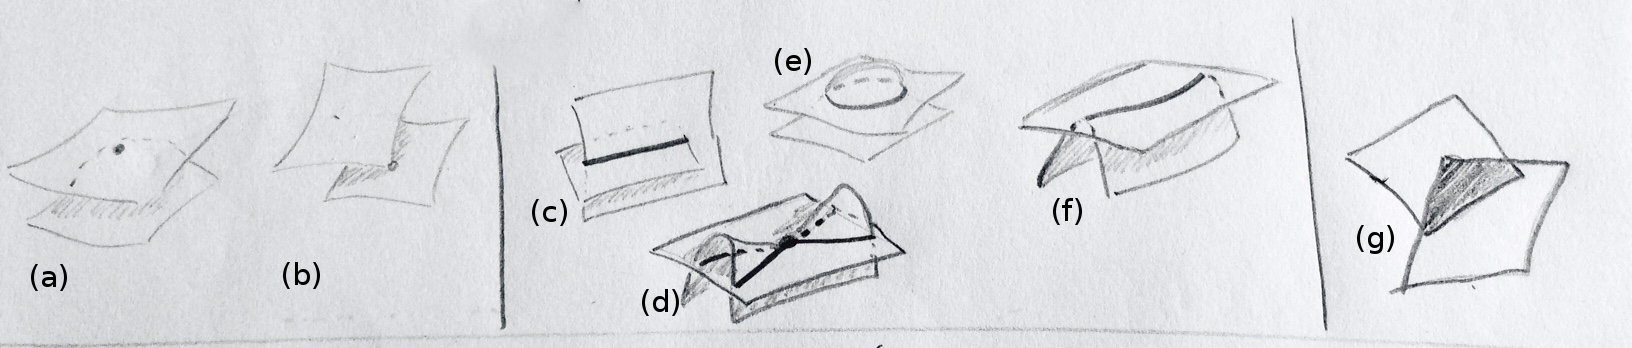
\includegraphics[width=0.95\textwidth]{cas_intersections_carreaux}
	\caption{Configurations possibles pour l'intersection de deux carreaux (non exhaustif).}
	\label{fig:config_intersection_carreaux}
\end{figure}


État de l'art des méthodes pour calculer l'intersection de carreaux paramétriques :
\begin{enumerate}
%	\item Analytiques : limité aux surfaces de degré algébrique très bas (\eg quadriques)
%	\item (Implicitisation (approchée) : )
	\item \anglais{Lattice}.\\
	Les méthodes de ce type consistent à calculer les intersections entre un réseau de \textit{courbes} iso-paramétriques d'un carreau et la \textit{surface} de l'autre carreau \cite{rossignac1987}. 
	Les points d'intersection obtenus sont ensuite connectés pour former les différentes courbes d'intersection. 
	Cette approche, qui présente l'avantage de réduire la complexité du problème, nécessite toutefois de choisir une résolution suffisamment fine pour le réseau des courbes iso-paramétriques afin de capturer correctement la topologie l'intersection. 
	En effet, si cette résolution est trop grossière, la méthode peut échouer à détecter certains détails tels que des points de contact isolés ou des petites boucles, qui apparaissent lorsque les carreaux s'intersectent de façon tangentielle ou quasi-tangentielle.
	
	\item Subdivision.\\
	Le principe de cette approche est de subdiviser de manière récursive le problème d'intersection original en plusieurs sous-problèmes --- typiquement des intersections de régions planes (\eg triangles) --- pour chacun desquels on peut aisément trouver la solution \cite{houghton1985}. 
	Ce type de méthodes produit ainsi un ensemble de segments de la courbe d'intersection, qui doivent également être connectés pour en former les branches. 
	Si la position des points d'intersection ainsi calculés peut être corrigée a posteriori afin de les ramener sur la véritable intersection des carreaux, les approximations utilisées ne garantissent pas la restitution exacte de la topologie de la courbe d'intersection, en particulier dans des cas d'intersections tangentielles ou quasi-tangentielles (illustration faux positif/faux négatif).
	Par ailleurs, le niveau élevé de précision requis par la plupart des applications en CAO nécessite un nombre de subdivisions souvent prohibitif, ce qui disqualifie les méthodes reposant uniquement sur la subdivision.
	%Toutefois, la combinaison de techniques de subdivision adaptative à d'autres méthodes locales de haute précision --- comme les méthodes dites de \textit{suivi} --- permet de concevoir des algorithmes de calcul d'intersection plus efficaces.
	%Les techniques de subdivision adaptative peuvent toutefois être utilisées 

	\item Suivi (\anglais{Marching}).\\
	Les méthodes dites de suivi cherchent dans un premier temps à trouver un point sur chaque branche de la courbe d'intersection. 
	Ensuite, elles procèdent au tracé de ces branches en marchant dans une direction indiquée par la géométrie différentielle locale de la courbe. 
	Afin d'identifier toutes les composantes connexes de la courbe d'intersection, il suffit de trouver les points où les branches ouvertes rencontrent le bord d'un des carreaux, ainsi que les paires de points critiques où les carreaux ont des directions normales parallèles.
	En effet, à chaque branche fermée de la courbe d'intersection est associée une telle paire de points \cite{sederberg1989}.
	En outre, tous les points singuliers de la courbe d'intersection (points de contact isolés, points \guillemets{doubles}, points de branchement) sont également des points critiques.
	\begin{itemize}
		\item trouver toutes les branches, sans doublons
		\begin{itemize}
			\item bords, points critiques
		\end{itemize}
		\item tracer (problème de Cauchy) avec un pas adéquat pour éviter saut/\anglais{jumping}, (\anglais{looping}) et marche-arrière /\anglais{backtracking} et s'arrêter au bon endroit
	\end{itemize}
\end{enumerate}
%pas de paramétrisation explicite (définition procédurale), méthode de Hohmeyer revisitée
%
%\begin{enumerate}
%	\item Subdivision : découper chaque surface en surfaces plus simple (\eg triangles) 
%	\item 
%\end{enumerate}

\par\bigskip

\begin{definition}
	Deux points $\p_1$ et $\p_2$ reposant respectivement sur les carreaux $\Sigma_1$ et $\Sigma_2$ forment une paire de \emph{points critiques} si, pour $i = 1,2$,
	\begin{equation}
		\crossprod{ \unv_{\Sigma_i}\!(\p_i) }{(\p_1 - \p_2)} = \vit{0}.
	\end{equation}
	(Ce sont en effet des points critiques (au sens où le gradient s'y annule) pour la fonction $(\p_1, \p_2) \mapsto \normtwo{\p_1 - \p_2}^2$.)
\end{definition}
\cite{yamaguchi1998} caractérise ces points (avec une autre fonction distance) et donne un algorithme pour tous les trouver




\subsection{Présentation/Vue d'ensemble/Caractéristiques de la méthode retenue}
Adaptation de la méthode préentée dans \cite{hohmeyer1992}, qui est centrée autour du théorème suivant

\begin{theoreme}[Hohmeyer]
	\label{theo:detection_boucles_hohmeyer}
	Soient $\Sigma_1$ et $\Sigma_2$ deux carreaux de continuité $\contdiff{1}$ dont les directions normales sont respectivement contenues dans les ensembles $\mathcal{N}_1$ et $\mathcal{N}_2$. \\
	S'il existe deux vecteurs $\vrm{p}_1$ et $\vrm{p}_2$ tels que, 
	pour tout $\unv_1 \in \mathcal{N}_1$ et pour tout $\unv_2 \in \mathcal{N}_2$,
	\begin{align}
		\dotprod{ \vrm{p}_1 }{ \unv_1 } > 0 &\text{\quad et\quad} \dotprod{ \vrm{p}_1 }{ \unv_2 } < 0, \label{eq:hohmeyer_separation}\\
		\dotprod{ \vrm{p}_2 }{ \unv_1 } > 0 &\text{\quad et\quad} \dotprod{ \vrm{p}_2 }{ \unv_2 } > 0, \label{eq:hohmeyer_hemisphere}
	\end{align}
	alors $\Sigma_1 \cap \Sigma_2$ n'est composée que de 
	\begin{itemize}
		\item points isolés situés sur le bord des carreaux ;
		\item segments ouverts qui ne contiennent ni point double ni point de branchement.
	\end{itemize}
	En outre, la direction tangente $\bt$ d'un tel segment vérifie en tout point
	\begin{equation}
		\dotprod{ \bt }{ (\crossprod{ \vrm{p}_1 }{ \vrm{p}_2 }) } > 0. \label{eq:hohmeyer_monotone}
	\end{equation}
\end{theoreme}


\begin{proof}
	\cf \cite[Théorème~4]{hohmeyer1992}
\end{proof}


Géométriquement, ce théorème peut s'interpréter de la manière suivante. 
D'une part, l'\autoref{eq:hohmeyer_separation} stipule que les ensembles $\mathcal{N}_1$ et $\mathcal{N}_2$ sont strictement séparables par un plan (passant par l'origine et orthogonal à $\vrm{p}_1$). 
D'autre part, l'\autoref{eq:hohmeyer_hemisphere} indique que $\mathcal{N}_1$ et $\mathcal{N}_2$ sont strictement contenus dans un même hémisphère (centré sur l'origine et centré autour du pôle $\vrm{p}_2$). 
Le \autoref{theo:detection_boucles_hohmeyer} donne ainsi une condition suffisante pour garantir que deux carreaux ne s'intersectent pas en une boucle fermée. 
Dans cette situation tous les points nécessaires à la détection de tous les éléments d'intersection (non singuliers) peuvent être trouvés en intersectant les bords de chaque carreau avec la surface de l'autre. 
De plus, l'\autoref{eq:hohmeyer_monotone} simplifie et garantit la validité du tracé des segments d'intersection. [\ldots]
%En effet, comme décrit dans \cite[Section~3.4]{hohmeyer1992}, le produit scalaire $\dotprod{ \bx }{ (\crossprod{ \vrm{p}_1 }{ \vrm{p}_2 }) }$ 
%%\begin{equation}
%%	w \defini{=} \dotprod{\bx}{\vrm{p}},
%%\end{equation}
%évolue de façon monotone le long du segment, ce qui permet d'éviter le phénomène de marche-arrière lorsqu'il est choisit comme paramètre.



\begin{enumerate}
	\item Détection des branches (composantes connexes) de la courbe d'intersection
	\begin{enumerate}
		\item Subdivision récursive des carreaux en régions qui
		\begin{itemize}
			\item sont clairement disjointes (test de séparation de volumes englobants \cite{eberly1999})
			\item ou bien s'intersectent de façon tangentielle
			\item ou bien ne peuvent pas s'intersecter en une boucle (critère d'élimination des boucles basé sur les enveloppes des normales basé sur le \autoref{theo:detection_boucles_hohmeyer})
		\end{itemize}
		\item Intersection entre les bords d'une région et la surface de l'autre, et vice versa (intersection arc-carreau)
		\item Subdivision récursive en régions qui
		\begin{itemize}
			\item sont clairement disjointes
			\item ne s'intersectent qu'en un seul segment transverse (pas de singularité), que l'on peut tracer sans ambiguïté (pas de saut d'une branche à l'autre)
		\end{itemize}
	\end{enumerate}
	

	\item Représentation des courbes d'intersection
	\begin{enumerate}
		\item le degré algébrique ainsi que le genre topologique des courbes solutions du système \eqref{eq:intersection_2_carreaux} augmentent tellement vite avec le degré des polynômes $\bs^i$ qu'il n'est pas envisageable de les représenter par des arcs paramétriques polynomiaux (\eg la courbe d'intersection de deux carreaux bi-cubiques est de degré 324 et de genre topologique 433 \cite{katz1988}).
		\item on a tout de même besoin d'un type de représentation permettant une évaluation précise des courbes d'intersection
		\item (compte tenu du niveau de précision exigé, une approximation paramétrique polynomiale globale ou \piecewise\ (spline) nécessiterait un volume excessif de données)
		\item on choisit donc d'adopter une représentation \textit{procédurale}
		\begin{enumerate}
			\item approximation linéaire par morceaux (polyligne) $(x,y,z,u_1,v_1,u_2,v_2)$
			\item on peut évaluer précisément n'importe quel point sur la courbe en évaluant d'abord la polyligne puis en raffinant le résultat de façon itérative (projection sur la véritable intersection)
			\item[$\Rightarrow$] un faible volume de données est stocké mais permet d'évaluer la courbe avec une précision arbitraire
		\end{enumerate}
	\end{enumerate}
	
	
	\item Tracé des courbes d'intersection
	\begin{enumerate}
		\item le critère d'élimination des boucles assure la monotonie de la paramétrisation de chaque segment d'intersection (pas de marche-arrière)
		\item problème aux limites (on connaît les deux extrémités du segment avant même de tracer la courbe) au lieu de problème de Cauchy (de valeurs initiales)
	\end{enumerate}
\end{enumerate}


\par\bigskip

Apports/modifications
\begin{enumerate}
	\item représentation des polynômes dans les bases de Bernstein \textit{et} Chebyshev (pour les arcs et carreaux) $\to$ on tire parti des avantages de chaque base pour les différentes étapes de l'algorithme :
	\begin{itemize}
		\item base de Bernstein (Bézier) 
		\begin{itemize}
			\item[+] propriété d'enveloppe convexe $\to$ tests de séparation
			\item[$\Rightarrow$] utilisée pour décrire localement les régions de carreau/arc
		\end{itemize}
		\item base de Chebyshev
		\begin{itemize}
			\item[+] évaluation efficace (Clenshaw) $\to$ méthodes itératives de type Newton qui nécessitent de nombreuses évaluations
			\begin{itemize}
				\item recherche/raffinement d'un point d'intersection arc-carreau
				\item recherche/raffinement d'une paire de points critiques
				\item raffinement d'un point d'intersection (entre 2 ou 3 carreaux)
			\end{itemize}
			\item[+] orthogonalité $\to$ économisation
			\item[+] FFT $\to$ (calcul du carreau pseudo-normal?)
			\item[$\Rightarrow$] utilisée pour décrire le carreau/arc \guillemets{racine}
		\end{itemize}
		\item changement de base par un produit matrice vecteur, matrice de passage donnée par \cite{rababah2003}
		\item on dérive des techniques pour les deux bases et pour les arcs et carreaux
		\begin{enumerate}
			\item extraction d'un bord de carreau sous la forme d'un arc
			\item subdivision : De Casteljau/\guillemets{Reparamétrisation affine}, généralisation de \cite{fournier1994} (cas particulier degré 3 et subdivision au milieu, \ie $u = v = 0$), à mettre en annexe
			\item boîtes englobantes orientées : heuristiques, \cite{munkberg2010} (Bernstein) et extension de \cite{campagna1997} (Chebyshev), à mettre en annexe et comparer complexité de construction et volume des boîtes)
		\end{enumerate}
	\end{itemize}
\end{enumerate}




\section{Intégration temporelle}
Suivi lagrangien de marqueurs (points de collocation, n\oe uds de la grille CGL)

\subsection{Advection dans champ de vecteur vitesse connu}
\begin{enumerate}
	\item Intégration explicite du vecteur vitesse des marqueurs lagrangiens (typiquement Runge-Kutta à l'ordre 4)
	\item Pas vraiment le cas dans les applications visées, mais on peut imaginer des situations de ce type (\eg déformation d'un solide sous l'effet d'efforts aérodynamiques $\to$ vitesse donnée par des solveurs de mécanique des structures/fluides)
\end{enumerate}



\subsection{Propagation suivant une vitesse normale donnée}
\subsubsection{Discrétisation de l'EdS propre d'un carreau paramétrique}
\label{section:discretisation_EdS_propre_carreau}
Entrée : vecteur position $\bx_{i,j}^{(k)}$ et vitesse normale $\nu_{i,j}^{(k)}$ de chaque marqueur lagrangien au $k$-ième instant, pas de temps $\Delta t$ (\ie $\rho = \nu \Delta t$)
\begin{enumerate}
	\item transformation directe (de l'espace physique vers l'espace spectral) pour construire les polynômes d'interpolation du vecteur position et de la vitesse normale
	\item construction des polynômes dérivés 
	\item transformation inverse pour évaluer les dérivées $\bsu$ et $\bsv$ aux n\oe uds CGL $(u_i,v_j)$
	\item calcul de la normale aux n\oe uds CGL
	\begin{equation}
		\unv = \unitized{\crossprod{\bsu}{\bsv}}
	\end{equation}
	\item calcul de la composante tangentielle du déplacement vers l'EdS propre aux n\oe uds CGL
	\begin{equation}
		\vrm{t} = \frac{
				\left( \nu_v I_{1,2} - \nu_u I_{2,2} \right) \bsu + 
				\left( \nu_u I_{1,2} - \nu_v I_{1,1} \right) \bsv
			}{
				I_{1,1} I_{2,2} - I_{1,2}^2
			}.
	\end{equation}
	\item on pose $\tau = \min\left\{\Delta t, \displaystyle\frac{\lambda}{\displaystyle\max_{i,j} \normtwo{\vrm{t}_{i,j}^{(k)} }} \right\}$ ($\lambda \leq 1$) et on avance dans le temps d'un pas $\tau$\\(ATTENTION : $\tau$ doit être le même pour tous les carreaux!)
	\begin{equation}
		\bx_{i,j}^{(k+1)} = \bx_{i,j}^{(k)} + \tau \nu_{i,j}^{(k)} 
		\left( 
			\tau \vrm{t}_{i,j}^{(k)} + \sqrt{1 - \tau^2 \normtwo{\vrm{t}_{i,j}^{(k)}}^2} \unv_{i,j}^{(k)}
		\right)
	\end{equation}
	
	\item Différence avec le simple transport suivant la normale
	\begin{itemize}
		\item on se bouge suivant la normale à l'EdS propre au lieu de la normale à l'interface
		\[
			\bx^{(k+1)} = \bx^{(k)} + \tau \nu^{(k)} \unv^{(k+1)}
		\]
		au lieu de 
		\[
			\bx^{(k+1)} = \bx^{(k)} + \tau \nu^{(k)} \unv^{(k)}
		\]
		$\sim$ schéma semi-implicite en temps?
		\[
			\sqrt{1 - y} = 1 + \bigO{y},
		\]
		donc
		\[
			\left( \bx^{(k+1)} - \bx^{(k)} \right) - \tau \nu^{(k)} \unv^{(k)} = \tau^2 \nu^{(k)} \vrm{t}^{(k)} + \bigO{\tau^3}
		\]
		et donc la différence est d'ordre 2 en temps
		\item si $\nu$ est uniforme (\ie $\nu_u = \nu_v = 0$) alors construire l'EdS propre revient à propager suivant la normale à l'interface courante. 
		En outre, la direction de $\unv$ reste constante en chaque point. 
		En revanche, le signe de $\unv$ peut s'inverser lorsque $\nu \tau$ dépasse le plus petit rayon de courbure local ($\to$ offset dégénéré \ldots).
	\end{itemize}
\end{enumerate}

\subsubsection{Discrétisation de la pseudo-EdS d'une arête \brep\ convexe}%d'un arc de courbe}
\begin{enumerate}
	\item \cf \autoref{section:parametrisation_pseudo_EdS_arete}
	\item paramétrisation polynomiale
	\begin{enumerate}
		\item[$\Rightarrow$] approximation (remarque sur les paramétrisations rationnelles exactes \cite{peternell1997})
		\item[$\Rightarrow$] degré à choisir
	\end{enumerate}
	\item décrire l'échantillonnage de la courbe d'intersection ($\Right{\bp}$, $\Left{\bp}$ et $\bg$) aux n\oe uds CGL pour le paramètre de Hohmeyer $w = \dotprod{\vrm{p}}{\bg}$
	\begin{enumerate}
		\item méthode procédurale : on s'appuie sur une polyligne et on affine par la méthode de Newton (expliciter l'itération)
		\item calcul de la direction tangente $\vrm{t} = \unitized{\bgw}$ (\cf géométrie différentielle des courbes d'intersection transverses, s'assurer de la positivité du produit scalaire avec le vecteur de paramétrisation de Hohmeyer $\vrm{p}$)
	\end{enumerate}
	\item évaluation des courbes \guillemets{limites} $\Right{\eos}$ et $\Left{\eos}$
	\item échantillonnage des arc caractéristiques aux n\oe uds CGL en $v \in \chebinterval$
	\begin{enumerate}
		\item en pratique, pour garantir la validité des courbes d'intersections tangentielles entre les carreaux de l'EdB, on choisit 
		\[
			\bo_i = \bg_i + \frac{\dotprod{\left( \Right{\eos}_i + \Left{\eos}_i - 2 \bg_i \right)}{\bt_i}}{2}\bt_i,
		\]  
		et, puisque $\lo{v} = -1$ et $\hi{v} = 1$,
		\[
			r_{i,j} = 
			\frac{
				\left(1 - v_j\right) \normtwo{\Right{\eos}_i - \bo_i} + \left(1 + v_j\right) \normtwo{\Left{\eos}_i - \bo_i}
			}{
				2
			},
		\]
		et
		\[
			\br_{i,j} = 
	        \cos\left( \frac{1 + v_j}{2} \theta_i \right) \Right{\br}_i +
	        \sin\left( \frac{1 + v_j}{2} \theta_i \right) \Right{\br}^{\perp}_i,
		\]
		\item[$\Rightarrow$] on a alors 
		\[
			\eos_{i,j} = \bo_{i} + r_{i,j} \br_{i,j}
		\]
	\end{enumerate}
	\item à noter qu'ici on n'utilise ni $\tau$ ni $\nu$
	\item les nouveaux carreaux ainsi créés seront ensuite propagés comme les autres aux instants suivants
\end{enumerate}



\subsubsection{Discrétisation de la pseudo-EdS d'un sommet \brep\ non-concave}
\begin{enumerate}
	\item polygone sphérique découpé en quadrilatères (\cf \autoref{section:quadrangulation_polygone_spherique})
	\begin{itemize}
		\item construction d'un carreau bilinéaire (échantillonnage aux n\oe uds de la grille CGL)
		\item projection sur la sphère
		\item[$-$] spectre de Chebyshev plus étalé (degré plus élevé pour une précision donnée)
	\end{itemize}
	\item ajustement de carreau sphérique à un nuage de points
	\begin{itemize}
		\item échantillonnage aux n\oe uds de la grille CGL du carreau obtenu par la méthode décrite dans la \autoref{section:ajustement_carreau_spherique}
		\item[$+$] spectre de Chebyshev plus compact
	\end{itemize}
\end{enumerate}




\section{Amélioration de la stabilité numérique}
\label{section:instabilités}

\subsection{Réduction de l'erreur d'aliasing}

méthode proposée par \cite{rahimian2015} difficile à appliquer dans notre cas car 
\begin{enumerate}
	\item les carreaux de surface ont un bord, 
	\item l'espacement non-uniforme des marqueurs lagrangiens (images des n\oe uds CGL) impose une forte contrainte CFL sur leurs déplacements
\end{enumerate}

\subsection{Prévention des singularités géométriques}
Notre approche permet naturellement de supporter les singularités géométriques de l'interface, à condition qu'elles soient localisées à l'intersection d'au moins deux carreaux de surface (et donc sur leur bord).
En revanche, les singularités qui se forment au sein d'un même carreau provoquent de sérieux problèmes de stabilité numérique.
On distingue 2 types de singularités (\cite[p.320]{patrikalakis2009}) :
\begin{itemize}
	\item points irréguliers (auto-intersection locale) (normale et plan tangent non définis, $\determinant{\fff} = 0$) $\Rightarrow$ oscillations de Gibbs
	\item auto-intersections globales (non-injectivité de la paramétrisation) : ne pose pas de problème de stabilité numérique mais viole la définition de variété
\end{itemize}

\begin{itemize}
	\item \cite{jiao2001} (en 2D, \ie l'interface est une courbe) : 
	\item \cite{farouki1986} donne les conditions pour qu'une interface (représentée par une mosaïque de carreaux paramétriques) propagée à vitesse normale uniforme devienne localement singulière
\end{itemize}

pistes de résolution envisageables
\begin{enumerate}
	\item approximation non dégénérée \cite{farouki1986}
	\item tracé des courbes iso-courbure critique \cite[chap.8]{patrikalakis2009} pour redéfinir les carreaux de surfaces concernés
	\item redécoupage des carreauxle long des courbes d'auto-intersection \cite{urick2019} 
	\begin{itemize}
		\item élimine les régions problématiques
		\item produit des nouveaux carreaux non-restreints
		\item (assure l'étanchéité de la mosaïque de carreaux)
	\end{itemize}
	
\end{enumerate}

%bilan : pas de solution simple, reste un gros point faible de l'approche choisie\ldots
bilan : en l'état actuel, problème non résolu mais idées solutions prometteuses

\chapter{Validation des méthodes numériques}

On s'intéresse d'abord à des cas de référence dans lesquels tous les carreaux ont un domaine paramétrique égal à $\chebinterval \times \chebinterval$, ce qui permet d'effectuer des mesures de précisions à la fois locales (position de l'interface) et globales (aire et volume délimité, par quadrature). 
Pour cela, on choisit des géométries simples et sans arête concave.
(On pourrait étendre les formules de quadrature aux carreaux restreints, voir IGA.)

\section{Propagation suivant un champ de vitesse analytique}

sphère dans un écoulement tourbillonnaire incompressible analytique de période temporelle $2T$
\begin{equation}
	\vrm{u}(x,y,z,t) = 
	%\cos \left( \frac{\pi t}{T} \right)
	\cos( \pi t/T )
	\colvec{
	\sin^2(\pi x) \left[ \sin(2\pi z) - \sin(2\pi y)\right] \\
\sin^2(\pi y) \left[ \sin(2\pi x) - \sin(2\pi z)\right] \\
\sin^2(\pi z) \left[ \sin(2\pi y) - \sin(2\pi x)\right]
	}.
\end{equation}

\begin{figure}
	\centering
	\setlength{\imagewidth}{0.49\linewidth}%
\newdimen\imypos
\imypos=1.1\imagewidth
\begin{tikzpicture}[%
	img/.style={anchor=north west, inner sep=0},%
	txt/.style={font=\normalsize, inner sep=2pt, anchor=south west}%
	]%
	%
	\begin{scope}%
	\clip(0,-0.15\imagewidth) rectangle (2\imagewidth, -2\imagewidth);
	\node[img] (im1) at (          0,         0) {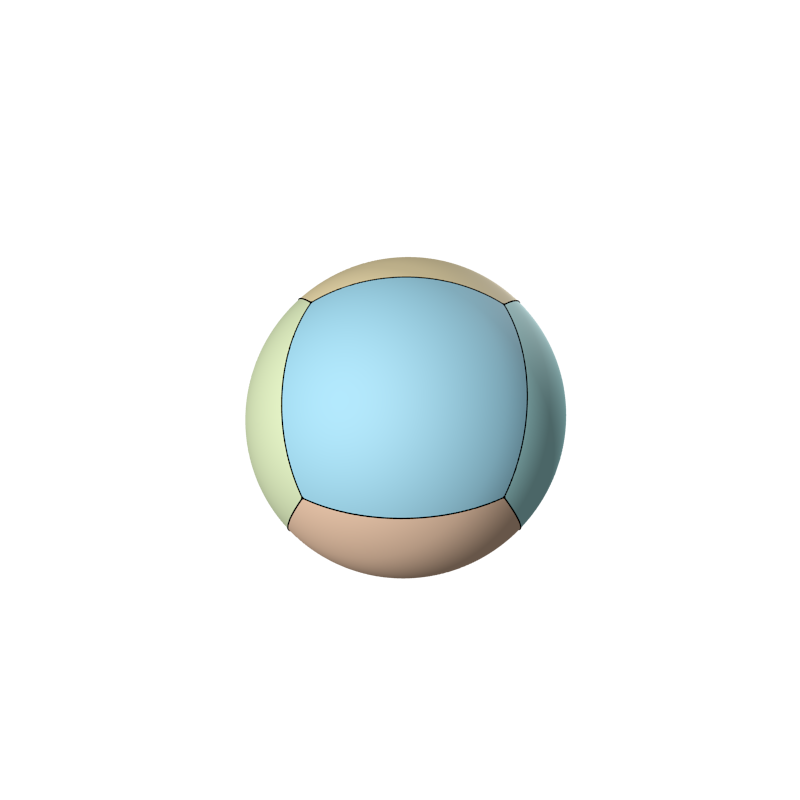
\includegraphics[width=\imagewidth]{vortex/snap_001}};
	\node[img] (im2) at (\imagewidth,         0) {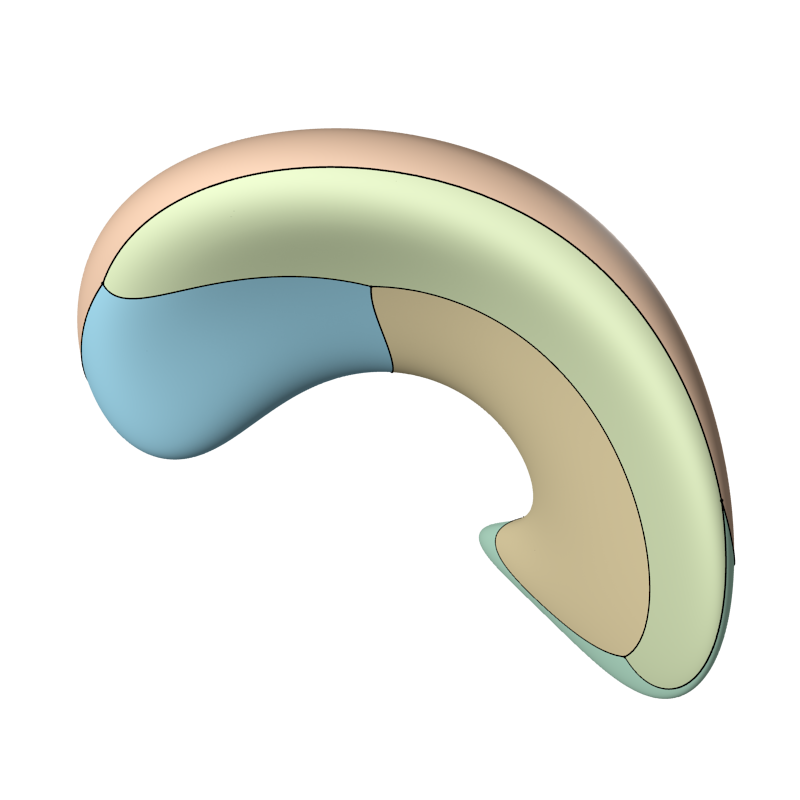
\includegraphics[width=\imagewidth]{vortex/snap_002}};
	\end{scope}%
	\node[img] (im3) at (          0,  -\imypos) {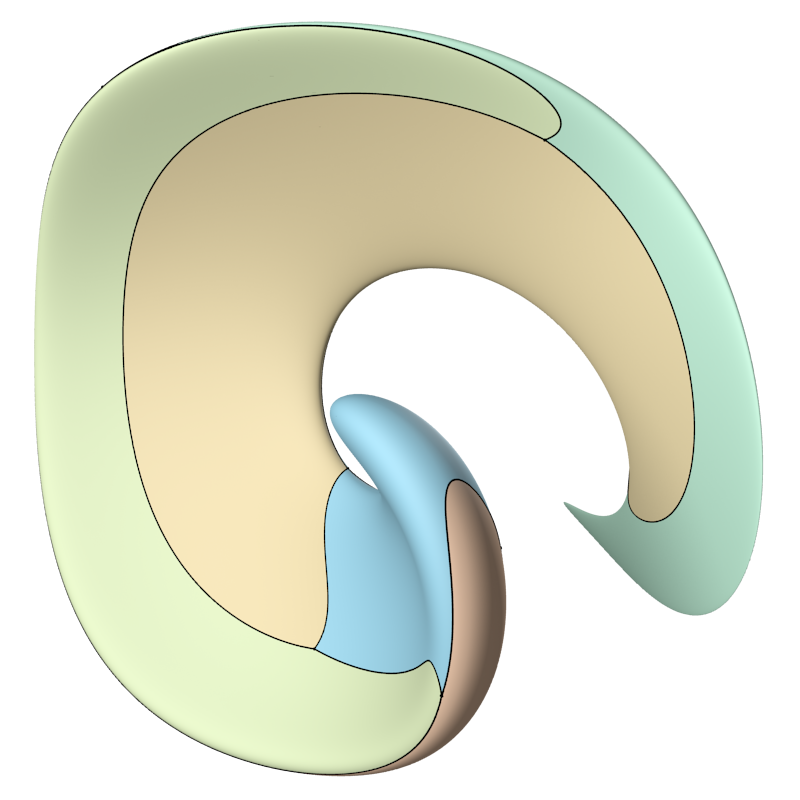
\includegraphics[width=\imagewidth]{vortex/snap_003}};
	\node[img] (im4) at (\imagewidth,  -\imypos) {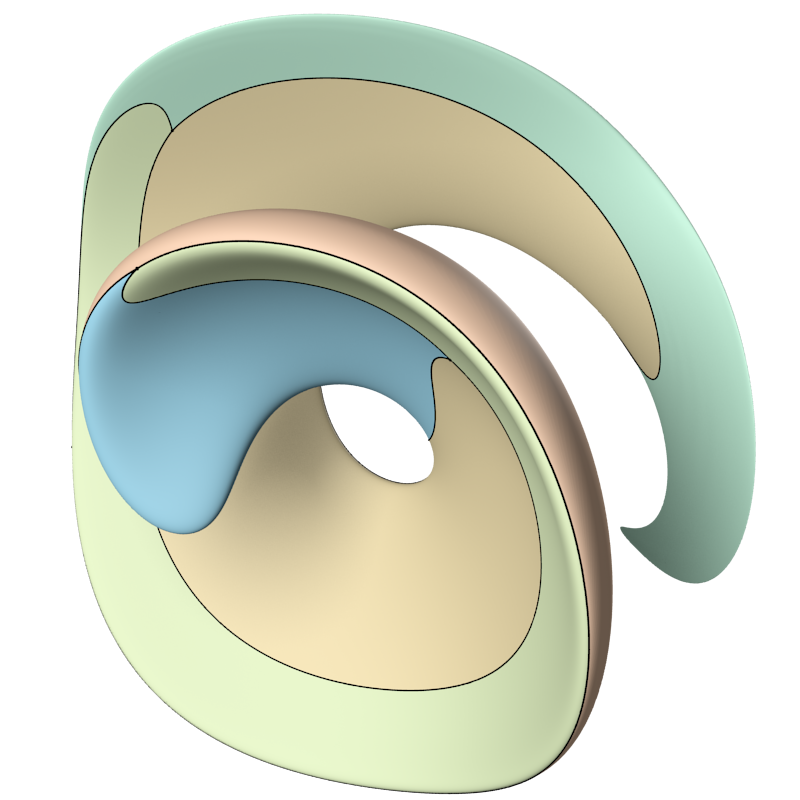
\includegraphics[width=\imagewidth]{vortex/snap_004}};
	\node[img] (im5) at (          0, -2\imypos) {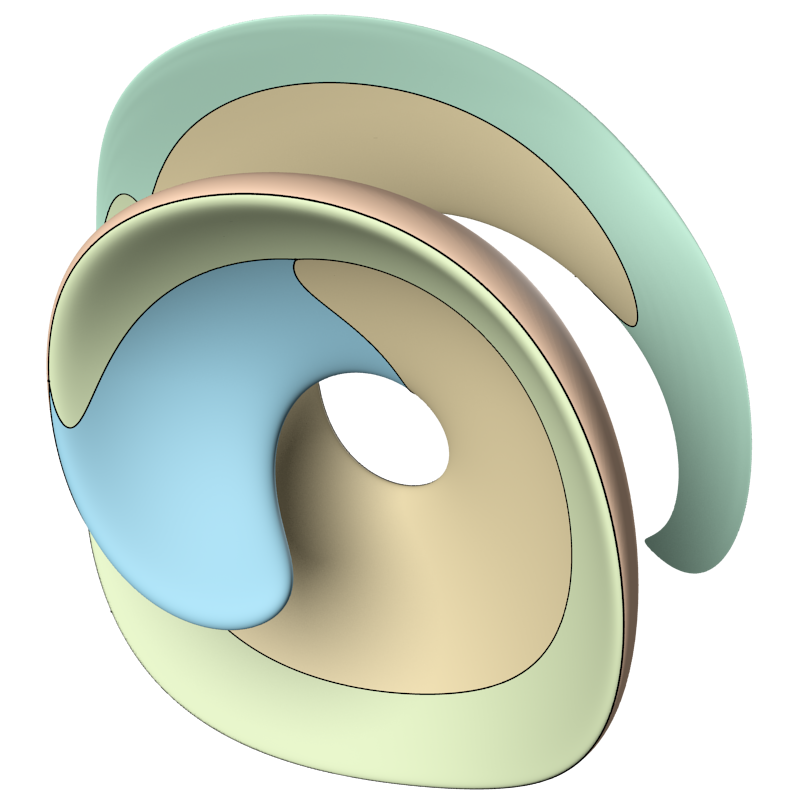
\includegraphics[width=\imagewidth]{vortex/snap_005}};
	\node[img] (im6) at (\imagewidth, -2\imypos) {\includegraphics[width=\imagewidth]{vortex/snap_006}};
	%
	\node[txt] at (im1.south west) {$t=   0$};
    \node[txt] at (im2.south west) {$t= T/8$};
    \node[txt] at (im3.south west) {$t= T/4$};
    \node[txt] at (im4.south west) {$t=3T/8$};
    \node[txt] at (im5.south west) {$t= T/2$};
    \node[txt] at (im6.south west) {$t=   T$};
\end{tikzpicture}
	\caption{Aperçu du modèle \brep\ de la sphère dans un écoulement tourbillonnaire à différents instants de la propagation ($T=4$).}
	\label{fig:snapshots_vortex}
\end{figure}

\begin{enumerate}
	\item paramétrisation initiale : grille CGL des faces d'un cube projetées sur la sphère% ou \guillemets{slerp}
	\item calcul de l'aire : intégration (approchée) par quadrature de Clenshaw-Curtis de l'élément d'aire $\sqrt{\determinant{\fff}}$
	\item calcul de volume : formule de Green avec quadrature exacte car l'intégrande est polynomiale %(étanchéité (continuité $\contgeom{0}$ partout) garantie car les marqueurs de bord coïncident tout au long de la déformation)
	\item critère d'erreur sur la position : distance à la sphère exacte
	\item convergence de l'erreur d'approximation sur la position (\autoref{fig:vortex_error_vs_dof_pos}), l'aire (\autoref{fig:vortex_error_vs_dof_air}) et le volume (\autoref{fig:vortex_error_vs_dof_vol}) à $t = 0$ et $t = T$ pour différents niveaux de discrétisations spatiale et temporelle 
	\begin{itemize}
		\item[$\to$] l'approximation de la sphère initiale converge rapidement avec le degré du polynôme d'interpolation(\ie le nombre de degrés de liberté)
		\item[$\to$] si la résolution spatiale est suffisamment fine, l'erreur d'approximation est essentiellement due à la discrétisation temporelle
	\end{itemize}
	\item convergence de la variation de volume au cours de la déformation (censée être nulle car $\nabla \cdot \vrm{u} = 0$) (\autoref{fig:vortex_error_volume_vs_time})
	\begin{itemize}
		\item[$\to$] on retrouve une convergence rapide : le pic à $t = T/2$ décroît exponentiellement avec $N$ 
	\end{itemize}
\end{enumerate}

%\\
%calcul de volume avec quadrature de Clenshaw-Curtis (exact, l'intégrande est polynomiale) (étanchéité (continuité $\contgeom{0}$ partout) garantie car les marqueurs de bord coïncident tout au long de la déformation)\\
%convergence de l'erreur d'approximation sur la position, l'aire et le volume à $t = 0$ et $t = T$ pour différents niveaux de discrétisations spatiale et temporelle\\

%%%%%%%%%%%%%%%%%%%%%%%%%%%%%
% FIGURES ERREUR VS DOF
\def\axw{0.48\textwidth}
\def\axh{0.39\textwidth}
\def\xlabl{$N$}%{$\mathrm{dof}$}
\def\ylabl{Erreur}
\def\xsep{2pt}
%%% POSITION
\plotVortexErrorVsDof{position}{la~}{pos}{maximale}
%%% AIRE
\plotVortexErrorVsDof{aire}{l'}{air}{relative}
%%% VOLUME
\plotVortexErrorVsDof{volume}{le~}{vol}{relative}
%%%%%%%%%%%%%%%%%%%%%%%%%%%%

%+ convergence de la variation de volume au cours de la déformation (censée être nulle)\\
\begin{figure}
  \centering
  \begin{tikzpicture}%
  \begin{semilogyaxis}[%
    axis lines*=left,%
    width=9cm, height=7cm,%
    xmin = 0.0, xmax = 1.0,%
    ymin = 1e-16, ymax = 1e0,%
    ytickten = {-16,-12,-8,-4,0},%
    xtick distance=.25,
    grid=major,%
    xlabel={$t/T$},%
    ylabel={$\frac{\left|V - V_0\right|}{V_0}$},%
    legend style={font=\small, at={(0.5,0.033)}, anchor=south},%
    no marks, each nth point=1]%
    \pgfplotstableread{figures/data/vortex/vortex_erreur_volume_vs_time_0.001.dat}{\datatable}
    \pgfplotstablegetcolsof{\datatable}
    \pgfmathtruncatemacro\numberofcols{\pgfplotsretval-1}
    \pgfplotsinvokeforeach{1,...,\numberofcols}{%
		\pgfplotstablegetcolumnnamebyindex{#1}\of{\datatable}\to{\colname}%
		\addplot+ table [y index=#1] from \datatable;% node[right, pos=1, anchor=west] {$N = \colname$};%
		\addlegendentryexpanded{$N = \colname$}%
    }%
  \end{semilogyaxis}%
  \end{tikzpicture}%
  \caption{Évolution au cours du temps de l'erreur relative en volume pour différents niveaux de discrétisation spatiale. Le schéma de Runge-Kutta explicite à l'ordre 4 est utilisé pour l'intégration temporelle, avec un pas de temps $\Delta t = 0.001$.}
  \label{fig:vortex_error_volume_vs_time}
\end{figure}

Nuancer la pertinence de ce cas test :
\begin{itemize}
	\item pour d'autres cas test analogues (\eg cas test de Enright), un mouvement tangentiel (reparamétrisation) des marqueurs lagrangiens est nécessaire pour garantir la stabilité numérique
	\item mais ce type de déformation extrême n'est pas celui que l'on vise dans nos applications, ce pourquoi on n'a pas plus considéré la reparamétrisation
	\item permet toutefois d'évaluer le pouvoir de résolution des polynômes de Chebyshev et vérifier la convergence rapide de l'erreur dapproximation
\end{itemize}

\section{Propagation à vitesse normale uniforme}
cube en expansion à vitesse normale uniforme $\nu = 1$

\begin{figure}
	\centering
	\newdimen\imwid
	\imwid=0.32\linewidth
	\begin{tikzpicture}
		\foreach [count=\i] \l in {{0}, {1}, {2}}
		{%
			\node (im\i) at (\i\imwid,0) {\includegraphics[width=\imwid]{expanding_cube/cube_brep_t\i}};
			\node[inner sep=0pt] (lab\i) at (im\i.south) {$t = \l$};
		}%
	\end{tikzpicture}
	\caption{Aperçu du modèle \brep\ du cube en expansion à différents instants de la propagation.}
	\label{fig:snapshots_cube}
\end{figure}

\begin{enumerate}
	\item stratégie pour la pseudo-EdS des sommets : polygone découpé en quads (\cf \autoref{section:quadrangulation_polygone_spherique}) pour évaluer simplement l'aire et le volume par quadrature (possible car $\nu$ est uniforme)
	\item critère d'erreur sur la position : erreur relative sur la distance au cube (car la solution exacte est une iso-surface de la fonction distance)
	\item convergence de l'erreur d'approximation sur la position, l'aire et le volume à $t = 2$ pour différents niveaux de discrétisations spatiale et temporelle (voir \autoref{fig:convergence_cube})
\end{enumerate}



\begin{figure}
	\centering
	\begin{tikzpicture}[inner frame sep=0]%
      \begin{semilogyaxis}[%
      %scale only axis,%
      axis lines*=left,%
      width=8cm, height=6cm,%
      xmin = 0, xmax = 20,% 
      ymin = 1e-16, ymax = 1,%
      xtick={0,5,10,15,20},%
      ytickten = {-16,-12,-8,-4,0},%
      grid=major,%both,%
      xlabel={$N$},%_{\mathrm{max}}$}, 
      ylabel={Erreur},%\ylabl},%
      legend style={font=\small},%
      legend pos=north east,%south west,%
      cycle list shift=0]%
	  \pgfplotstableread{figures/data/convergence_expanding_cube.dat}  {\datatable}%
	  \pgfplotstablegetcolsof{\datatable}%
      \pgfmathtruncatemacro\numberofcols{\pgfplotsretval-1}%
      \pgfplotsinvokeforeach{3,...,\numberofcols}{%
        \pgfplotstablegetcolumnnamebyindex{#1}\of{\datatable}\to{\colname}%
        %https://tex.stackexchange.com/questions/317225/automatic-labelling-of-isolines-based-on-tables-column-name
		\addplot table [x index=0, y index=#1] from \datatable;
  	    \addlegendentryexpanded{\colname}%
      }%
      \end{semilogyaxis}%
    \end{tikzpicture}%
	\caption{Erreurs sur la position l'aire et le volume pour différents niveaux de discrétisations spatiale et temporelle, à $t = 2$.}
	\label{fig:convergence_cube}
\end{figure}

Intérêts de ce cas test :
\begin{itemize}
	\item valider l'approximation du vecteur normal unitaire 
	\item valider la construction des pseudo-EdS des arêtes et sommets \brep\ convexes
\end{itemize}

%\include{mainmatter/chap3...}
\mypart{Seconde}{Intégration de l'outil de suivi de surface dans une chaîne de calcul multi-physique}

%\chapter{Déformation de maillage surfacique}

\textit{Objectif du chapitre: on veut mettre au point une méthodologie pour déformer un maillage de l'interface en propagation en utilisant le modèle \brep\ dynamique comme support géométrique, afin de pouvoir réaliser des simulations EF/VF dans des domaines de géométrie déformables.}

%Simulations en 3d nécessitent maillage volumique dont l'interface représente la frontière déformable

\section{État de l'art}
\subsection{Simulation numérique dans une géométrie déformable}
maillage volumique conforme (body-fitted + ALE, Chimère/FLUSEPA) / non-conforme (IBM \ldots)\\

\subsection{Génération de maillage surfacique basé sur un modèle \brep}
\begin{itemize}
	\item méthodes indirectes (\ie Riemanniennes)
	\begin{itemize}
		\item face par face \cite{borouchaki2000}
		\item paramétrisation globale \cite{marcum1999, noel2002, jones2004}
	\end{itemize}
	\item méthodes (frontales) directes \cite{foucault2013}
\end{itemize}

\subsection{Optimisation/Adaptation de maillage surfacique}
\begin{itemize}
	\item changements locaux de connectivité
	\begin{itemize}
		\item bascule d'arête
		\item contraction d'arête
	\end{itemize}
	\item bouger de n\oe ud (direct, \ie $xyz$ ou indirect, \ie $uv$)
	\begin{itemize}
		\item méthodes heuristiques (lissage laplacien, analogies physiques \cite{farhat1998}, interpolation (IDW, RBF, \ldots) \ldots)
		\item lissage basé sur l'optimisation d'une métrique de qualité \cite{freitag1995, canann1998, jiao2008, gargallo2014}
	\end{itemize}
\end{itemize}

\section{Problématiques}
contraintes :
\begin{enumerate}
	\item ALE $\Rightarrow$ préserver la connectivité du maillage autant que faire se peut (\ie déformation pure)
	%\item le maillage doit représenter fidèlement l’interface (⇒ sommets localisés exactement sur la surface BRep) et ses caractéristiques géométriques (arêtes vives, coins, . . . ) (⇒ contraintes sur les nœuds et arêtes du maillage dans ces régions) (→ persistance des entités BRep?)
	\item \label{item:maillage_fidele} le maillage doit être une approximation géométrique fidèle de l’interface (dont la géométrie \guillemets{exacte} est définie par le modèle \brep)
	\begin{itemize}
		\item solution la plus simple : le maillage interpole la surface \brep\ aux n\oe uds (qui sont alors localisés sur des entités \brep\ et donc sur un ou plusieurs carreaux de surface) $\Rightarrow$ l'écart de corde doit être contrôlé (taille d'élément dicté par le rayon de courbure local, maillage explicite des caractéristiques/singularités géométriques (arêtes vives, coins, \ldots))
	\end{itemize}
	\item maintenir une bonne qualité de maillage (métrique à définir suivant la méthode de calcul) $\Rightarrow$ lissage/optimisation (par déplacements tangentiels pour respecter la contrainte \ref{item:maillage_fidele})
\end{enumerate}


\subsection{Lien entre le maillage et le modèle \brep}
(Solution à la contrainte \ref{item:maillage_fidele})\par
A chaque n\oe ud du maillage sont associés
\begin{itemize}
	\item un pointeur vers l'entité \brep\ qui le supporte (sommet, arête ou face)
	\item un jeu de coordonnées paramétriques (\ie un point $(u,v)$ pour chaque carreau de surface associé à l'entité \brep\ de support)\footnote{Rappel : les courbes d'intersection ne sont pas paramétrisées directement mais évaluées de manière procédurale en interrogeant les deux carreaux de surface concernés. Les points d'intersection (qui décrivent les sommets \brep) sont repérés dans l'espace paramétrique de chaque carreau de surface concerné.}
\end{itemize}
Les coordonnées $(x,y,z)$ d'un n\oe ud sont alors obtenues en évaluant un ou plusieurs carreaux de surfaces, ce qui garantit que le n\oe ud repose exactement sur la surface \brep\ (à condition que les coordonnées $(u,v)$ soient situées à l'intérieur ou sur le bord du domaine paramétrique des faces \brep\ concernées).


\section{Déformation de maillage conforme aux faces \brep}
\subsection{Limitations}
\begin{itemize}
	\item les arêtes \brep\ douces introduisent des contraintes supplémentaires sur le maillage, sans avoir de signification du point du vue du calcul EF/VF $\Rightarrow$ éléments de mauvaise qualité
	\item problème de la persistance des entités \brep
\end{itemize}
$\Rightarrow$ maillage \textit{trans-carreaux}


\section{Déformation de maillage trans-carreaux}
\subsection{Construction d'une structure d'hypergraphe}
Structure intermédiaire qui conserve la définition du modèle \brep\ sous-jacent \cite{foucault2008}\\
Faces adjacentes qui forment une région surfacique de continuité \contgeom{1} rassemblées dans une \textit{hyper-face}\\
Arêtes adjacentes qui forment une branche de courbe de continuité \contgeom{1} rassemblées dans une \textit{hyper-arête}\\
Les n\oe uds du maillage peuvent traverser les arêtes douces intérieures à une hyper-face\\
Les hyper-arêtes sont des listes chaînées de (co-)arêtes \brep\ (potentiellement cycliques).
Dans le maillage, elles sont matérialisées par des chaînes d'arêtes dont les n\oe uds sont contraints (1 seul degré de liberté pour les n\oe uds intérieurs, 0 pour les éventuels n\oe uds aux extrémités)

\subsection{\guillemets{Transition} d'un instant au suivant}

\subsubsection{Correspondance des hypergraphes}
\guillemets{événements} possibles 

\subsubsection{Régénération du maillage contraint}%des hyper-arêtes}
\begin{itemize}
	\item n\oe uds avec 0 degré de liberté $\to$ coordonnées $(x,y,z)$ du sommet \brep\ associé (\guillemets{coin})
	\item n\oe uds avec 1 degré de liberté $\to$ régénération des chaînes (hyper-arêtes)
\end{itemize}

\subsubsection{\guillemets{Pré-déformation}}

\subsection{Optimisation de maillage trans-carreaux}
méthode directe avec re-projection sur hyper-face/arête
\chapter{Adaptation d'un maillage de surface dynamique}

\textit{Objectif du chapitre: on veut mettre au point une méthodologie pour déformer un maillage de l'interface en propagation en utilisant le modèle \brep\ dynamique comme support géométrique, afin de pouvoir réaliser des simulations EF/VF dans des domaines de géométrie déformable.}

\par\bigskip

Motivation
\begin{enumerate}
	\item les méthodes (EF, VF, \ldots) employées pour la simulation numérique nécessitent un \textit{maillage} du domaine de calcul
	\item la précision et la vitesse de convergence du calcul dépendent fortement de la qualité (forme et taille) des éléments du maillage
	\item on 
\end{enumerate}

\section{Problématique et état de l'art}

\subsection{Simulation numérique dans un domaine à géométrie déformable}
\begin{enumerate}
	\item maillage volumique (fluide) conforme à l'interface
	\begin{enumerate}
		\item \label{item:methodo_bodyfitted_ALE} 1 seul maillage \anglais{body-fitted} avec formulation ALE \emph{(ref)}
		\begin{itemize}
			\item principe : frontière = maillage de l'interface, intérieur déformé de façon arbitraire
			\item intérêt/avantages : \ldots
			\item contraintes/inconvénients : 
			\begin{itemize}
				\item la qualité du maillage volumique dépend fortement de celle du maillage surfacique, surtout dans les régions proches de l'interface, où ont généralement lieu les phénomènes physiques les plus pertinents
				\item la connectivité du maillage doit rester fixe \emph{(à vérifier)}
			\end{itemize}
		\end{itemize}
		
		\item plusieurs maillages \anglais{body-fitted} qui se superposent
		\begin{itemize}
			\item méthode Chimère \cite{meakin1989, wang2000}, FLUSEPA \cite{brenner1991}
			\item intérêt/avantages : 
			\begin{itemize}
				\item facilite la génération du maillage volumique lorsque la géométrie est complexe (\eg hyper-sustentateurs)
				\item évite de déformer un maillage 3d
			\end{itemize}						
			\item contraintes/inconvénients : 
			\begin{itemize}
				\item nécessite de traiter les intersections entre les blocs de maillage
				\item limité aux mouvements rigides \emph{(à vérifier)}
			\end{itemize}
		\end{itemize}
	\end{enumerate}
	
	\item maillage volumique non-conforme à l’interface
	\begin{itemize}
		\item méthode des frontières immergées \cite{peskin2002, hovnanian2012, wang2012} : interface représentée explicitement, volume (fluide) traité de façon eulérienne (\ie maillage fixe)
		\item intérêt/avantages : évite de générer et déformer un maillage 3d autour d’une géométrie complexe
		\item contraintes/inconvénients : application indirecte des conditions aux limites
	\end{itemize}
\end{enumerate}

Dans cette thèse,
\begin{enumerate}
	\item on ne traite que le maillage (surfacique) de l'interface
	\item on se concentre sur des maillages triangulaires linéaires par morceaux, mais une extension aux maillages hybrides et courbes (high-order) est envisageable
\end{enumerate}






\subsection{Génération de maillage surfacique basé sur un modèle \brep}
Essentiellement extension de méthodes standard (\ie quadtree, Delaunay, avancée de front) 2d plan à des surfaces immergées/plongées dans $\reals^3$
\begin{enumerate}
	\item méthodes indirectes (Riemanniennes) : on travaille dans l'espace paramétrique en tenant compte de la métrique (anisotrope, Riemannienne) induite par la paramétrisation de façon à ce que le plongement du maillage dans $\reals^3$ respecte les critères prescrits
	\begin{enumerate}
		\item conforme à la topologie \brep\ : on exploite directement les paramétrisations locales (carreaux de surface) du modèle \brep\ \cite{borouchaki2000} (on maille d'abord les sommets, puis les arêtes et enfin les faces afin de garantir la conformité du maillage)
		\begin{itemize}
			\item intérêt/avantages : utilisation de méthodes 2d plan robustes et efficaces
			\item contraintes/inconvénients : les arêtes \brep\ douces introduisent des contraintes supplémentaires sur le maillage, sans avoir de signification du point du vue du calcul EF/VF $\Rightarrow$ éléments de mauvaise qualité
		\end{itemize}
		\item trans-carreaux par (re-)paramétrisation globale : 
			\begin{enumerate}
				\item \cite{marcum1999} :
				\begin{enumerate}
					\item on construit d'abord un maillage de référence conforme à la topologie \brep\ d'un ensemble de faces regroupées
					\item \label{item:bouche_trous} on bouche artificiellement les éventuels \guillemets{trous} afin qu'il n'y ait qu'un seul bord
					\item on plonge ce maillage dans un espace paramétrique global :
					\begin{itemize}
						\item afin d'obtenir les coordonnées paramétriques globales des n\oe uds intérieurs, on résout un système d'équations elliptique (opérateur Laplacien combinatoire) avec une condition de Dirichlet pour fixer les n\oe uds du bord sur un cercle
						\item on modifie les coordonnées paramétriques globales des n\oe uds du bord afin d'améliorer la forme des éléments incidents
						\item (on répète le processus jusqu'à ce que la qualité des éléments dans l'espace paramétrique global soit convenable)
					\end{itemize}
					\item on élimine les éventuels éléments fictifs créés à l'étape \ref{item:bouche_trous}
					\item on génère un maillage dans l'espace paramétrique global par avancée de front en utilisant le maillage de référence comme approximation géométrique dans l'espace physique
					\item on retrouve les coordonnées paramétriques locales des n\oe uds du nouveau maillage 
				\end{enumerate}
				\item \cite{noel2002} : 
				\begin{enumerate}
					\item le domaine paramétrique de chaque face \brep\ est décomposé en cellules triangulaires s'appuyant sur les contours
					\item chaque cellule (courbe) est en bijection avec un triangle (linéaire) dans l'espace paramétrique global
					\item un maillage du domaine paramétrique global est généré (quadtree-Delaunay) 
				\end{enumerate}
				\item \cite{jones2004} : ?%on part d'un maillage de référence conforme à la topologie \brep. On choisit une face \brep\ de \textit{base}, dont l'espace paramétrique local sert de base pour construire un espace paramétrique global. Les faces \brep\ adjacentes sont ensuite plongées dans l'espace paramétrique global . Cette approche ne fonctionne que lorsque les domaines paramétriques des faces adjacentes ont des dimensions similaires
			\end{enumerate}
		\begin{itemize}
			\item intérêt/avantages : lève les contraintes topologiques du modèle \brep\ qui ne sont pas pertinentes pour le calcul EF/VF
			\item contraintes/inconvénients : 
			\begin{itemize}
				\item topologie : limité aux variétés avec un ou plusieurs bords $\Rightarrow$ nécessite un découpage (généralement manuel) de l'interface
				\item géométrie : limité aux surfaces quasi-planes et régulières
				\item (méthodes pas suffisamment automatisées)
			\end{itemize}
			
		\end{itemize}
	\end{enumerate}
	
	\item méthodes directes : 
	\begin{enumerate}
		\item \cite{lau1996} : avancée de front directement dans $\reals^3$ avec projection sur la surface exacte des n\oe uds au cours de la génération $\to$ limité à une paramétrisation continue (\ie carreau par carreau)
		\item \cite{foucault2013} : avancée de front directe trans-carreaux
	\end{enumerate}
\end{enumerate}







\subsection{Optimisation de maillage surfacique}
\begin{figure}
\centering
\includegraphics[width=\textwidth]{operations_locales_optimisation_maillage}
\caption{\ldots}
\label{fig:operations_locales_optimisation_maillage}
\end{figure}

\begin{enumerate}
	\item bouger de n\oe ud (direct, \ie $xyz$ ou indirect, \ie $uv$)
	\begin{enumerate}
		\item méthodes heuristiques (lissage laplacien, analogies physiques \cite{farhat1998}, interpolation (IDW, RBF, \ldots) \ldots)
		\item lissage basé sur l'optimisation d'une métrique de qualité \cite{freitag1995, canann1998, jiao2008} \cite{gargallo2014} $\to$ maillage supporté sur un carreau de surface paramétrique
	\end{enumerate}
	\item changements locaux de connectivité
	\begin{enumerate}
		\item bascule d'arête
		\item contraction d'arête
		\item scission d'arête
	\end{enumerate}
\end{enumerate}

%Dans cette thèse,
%\begin{enumerate}
%	\item (\autoref{item:methodo_bodyfitted_ALE})/de nombreux codes de calculs ne tolèrent pas les changement de connectivité en cours de calcul $\Rightarrow$ on se concentre essentiellement sur le bouger de n\oe ud (déformation pure) 
%	\item on n'effectuera des reconnections locales qu'en dernier recours (remaillage)
%\end{enumerate}



\par\bigskip
le maillage doit être une approximation géométrique fidèle de l’interface (dont la géométrie
« exacte » est définie par le modèle \brep)\\
$\to$ solution la plus simple : le maillage interpole la surface \brep\ aux n\oe uds (qui sont alors localisés sur des entités \brep\ et donc sur un ou plusieurs carreaux de surface) $\Rightarrow$ l'écart de corde doit être contrôlé (taille d'élément dicté par le rayon de courbure local, maillage explicite des caractéristiques/singularités géométriques (arêtes vives, coins, \ldots))


\section{Lien entre modèle \brep\ et maillage trans-carreaux}
Objectifs :
\begin{enumerate}
	\item \label{item:limiter_ecart_corde} représenter fidèlement la surface (courbe) à l'aide d'un maillage (linéaire) (\ie limiter/contrôler l'écart de corde)
	\item \label{item:alleger_contraintes_topo} s'affranchir au maximum des contraintes sur le maillage inutilement imposées par la topologie du modèle \brep\ (arêtes douces)
	
\end{enumerate}

\subsection{Construction d'une structure d'hypergraphe}


\section{Déformation de maillage trans-carreaux basé sur un modèle \brep\ dynamique}
Objectifs :
\begin{enumerate}
	\item \label{item:preserver_connect} préserver autant que faire se peut la connectivité du maillage (éviter de générer un nouveau maillage à chaque pas de temps)
\end{enumerate}

\subsection{Correspondance d'hypergraphes}


\subsection{Régénération du maillage contraint}

\subsection{\anglais{Untanglement}}

\subsection{Optimisation par bouger de n\oe ud}
\label{section:projection_surface_composite}
Décrire la procédure de projection d'un déplacement sur la surface \brep\ (sur une hyper-face ou une hyper-arête)
$\rightarrow$ trajectoire trans-carreaux \cite[Section~5.5]{foucault2008}), \cite{thompson2005}, \cite[p.42 et Section~4.4.1]{crozet2017}

\subsection{Optimisation par reconnections locales}
\subsubsection{Bascule d'arête}
Les arêtes contenues dans les chaînes ne peuvent pas être basculées.

\subsubsection{Contraction d'arête}
Soit $e$ l'arête entre les n\oe uds $p_1$ et $p_2$. Sans restreindre la généralité, on supposera que $\ddl(p_1) \leq 
\ddl(p_2)$.
Ici, $\ddl(p)$ représente le nombre de degrés de liberté du n\oe ud $n$, \ie 
\begin{itemize}
	\item $\ddl(p) = 0$ si $n$ est contraint sur un sommet \brep\ ;
	\item $\ddl(p) = 1$ si $n$ est contraint sur une hyper-arête (chaîne) ;
	\item $\ddl(p) = 2$ si $n$ n'est pas contraint (ou plutôt est contraint sur une hyper-face).
\end{itemize}
Si $\ddl(p_1) = \ddl(p_2) = 1$, la contraction n'est possible que si $e$ fait partie d'une chaîne, \ie les n\oe uds $p_1$ et $p_2$ sont contraints sur la même hyper-arête (voir \autoref{fig:contraction_arete_cas_1_1}).

\setlength{\imagewidth}{50mm}
\begin{figure}
  \centering
  %
  \hspace*{\fill}
  \subbottom[L'arête $e_2$ peut être contractée, mais pas $e_1$ puisque ses extrémités sont contenues dans deux chaînes distinctes (en rouge et vert).]{
	\includegraphics[width=\imagewidth]{contraction_arete_cas_1_1_avant}
	\label{fig:contraction_arete_cas_1_1_avant}
  }
  \hfill%
  \subbottom[Maillage résultant de la contraction de l'arête $e_2$.]{
	\includegraphics[width=\imagewidth]{contraction_arete_cas_1_1_apres}
	\label{fig:contraction_arete_cas_1_1_apres}
  }
  \hspace*{\fill}
  \caption{Deux cas possibles pour une arête dont les deux sommets ont un seul degré de liberté.}
  \label{fig:contraction_arete_cas_1_1}
  %
\end{figure}

Si $\ddl(p_1) < \ddl(p_2)$ on contracte $e$ vers le n\oe ud $p_1$. 
Si $\ddl(p_1) = \ddl(p_2)$ on contracte $e$ vers son milieu. Afin de localiser précisément ce milieu sur la surface \brep\ (\ie connaître l'entité \brep\ qui le supporte, ainsi que ses coordonnées paramétriques dans les carreaux de surface concernés), on calcule la projection sur la surface \brep\ du n\oe ud $p_1$ translaté d'un vecteur $\frac{p_2 - p_1}{2}$ (voir \autoref{fig:contraction_arete_milieu}), en suivant la procédure décrite dans la \autoref{section:projection_surface_composite}.

\setlength{\imagewidth}{50mm}
\begin{figure}
  \centering
  \includegraphics[width=\imagewidth]{contraction_arete_milieu}
  \caption{Placement du n\oe ud résultant de la contraction d'une arête. Le $\ddl$ de chaque n\oe ud concerné est indiqué à côté de celui-ci. Les flèches représentent les vecteurs déplacement à projeter pour chaque arête contractée.}
  \label{fig:contraction_arete_milieu}
\end{figure}


\subsubsection{Scission d'arête}
On insère un n\oe ud au milieu d'une arête. Comme pour la contraction d'arête, les coordonnées de ce milieu sont une nouvelle fois obtenue par la procédure de projection décrite dans la \autoref{section:projection_surface_composite}.
Cette fois, la projection du déplacement se fait en partant du sommet de l'arête ayant le plus grand nombre de degrés de liberté, comme illustré sur la \autoref{fig:scission_arete_milieu}.

\setlength{\imagewidth}{50mm}
\begin{figure}
  \centering
  \includegraphics[width=\imagewidth]{scission_arete_milieu}
  \caption{Placement du nouveau n\oe ud résultant d'une scission d'arête. Le $\ddl$ de chaque n\oe ud concerné est indiqué à côté de celui-ci. Les flèches représentent les vecteurs déplacement à projeter pour chaque arête scindée.}
  \label{fig:scission_arete_milieu}
\end{figure}





%%%%%%%%%%%%%%%%%


%% ANNEXES %%
\appendix


%%%%%%%%%%%%%%%%%



%% BIBLIOGRAPHIE %%
\backmatter
\cleardoublepage
\phantomsection
\nocite{*}% à retirer à la fin!!!
\bibliographystyle{mybibstyle}
\bibliography{biblio/spectral_chebyshev,biblio/mesh_generation,biblio/mesh_optimization,biblio/cad,biblio/deformable_geometry,biblio/interface_propagation,biblio/intersection,biblio/computational_geometry,biblio/offsets.bib}
%%%%%%%%%%%%%%%%%


\end{document}
